\chapter{Results} % Main appendix title
\label{Appendix-results} % For referencing this appendix elsewhere, use 
In this chapter we document results, based on the methodology used.

\section{CARLA Simulator results}
In this section we document simulation results, describing the code repository commit hash, and any relevant commands and outputs.

\subsection{Run 001 - Installing Carla with apt-get}

We installed Carla following procedure described in:

\begin{verbatim}
https://carla.readthedocs.io/en/0.9.13/start_quickstart/#carla-installation
\end{verbatim}

i.e. with apt-get. The startup procedure differs in that we do not use 
Unreal Engine directly, though the assumption is, it must be installed.
The version can be seen in the dist sub-directory:

\begin{verbatim}
)$ ls -l /opt/carla-simulator/PythonAPI/carla/dist/
total 119796
-rw-r--r-- 1 root root 32244452 Nov 17  2021 
carla-0.9.13-cp27-cp27mu-manylinux_2_27_x86_64.whl
-rw-r--r-- 1 root root 29700064 Nov 17  2021 
carla-0.9.13-cp37-cp37m-manylinux_2_27_x86_64.whl
-rw-r--r-- 1 root root 31615292 Nov 15  2021 
carla-0.9.13-py2.7-linux-x86_64.egg
-rw-r--r-- 1 root root 29102504 Nov 15  2021 
carla-0.9.13-py3.7-linux-x86_64.egg
\end{verbatim}

NB additional required packages must be installed:

\begin{verbatim}
cd PythonAPI\examples
python3 -m pip install -r requirements.txt    
\end{verbatim}

Running is the same as with cloning the app:

\begin{verbatim}
$ git clone https://github.com/carla-simulator/carla.git
$ cd carla
$ ./CarlaUE4.sh
\end{verbatim}

With apt-get install:

\begin{verbatim}
$ cd /opt/carla-simulator/
$ ./CarlaUE4.sh
\end{verbatim}

To generate traffic and weather, scripts are in same location in both cases above:

\begin{verbatim}
$ cd /PythonApi/examples
$ python generate_traffic.py -n 60 -w 100 
# On A different shell
$ python dynamic_weather.py --speed 0.05 
# On a different shell
$ python automatic_control.py
# On a different shell
\end{verbatim}

Optional parameters may be passed to the start-up script:

\begin{verbatim}
$ ./CarlaUE4.sh -carla-server -benchmark -fps=15 -windowed -ResX=800 -ResY=600
\end{verbatim}

e.g. for a set frame rate and window size.

%% ROS Bridge for later


%%%%%%%%%%%%%%%%%%%%%%%%%%%%%%%%%%%%%%%%%%%%%%%%%%%%%%%%%%%%%%%%%%%%%%%%%%%%%
% RUN XXX - TEMPLATE - experiment log template
%%%%%%%%%%%%%%%%%%%%%%%%%%%%%%%%%%%%%%%%%%%%%%%%%%%%%%%%%%%%%%%%%%%%%%%%%%%%%
%\subsection{Run XXX -  }
%\label{app_res:XXX}
%\begin{verbatim}
%Commit:
%Model: 
%Outputs: 
%Dataset: 
%Command:
%Environment: 
%Comment: 
%\end{verbatim}

%%%%%%%%%%%%%%%%%%%%%%%%%%%%%%%%%%%%%%%%%%%%%%%%%%%%%%%%%%%%%%%%%%%%%%%%%%%%%
% RUN 001 - Running CARLA
%%%%%%%%%%%%%%%%%%%%%%%%%%%%%%%%%%%%%%%%%%%%%%%%%%%%%%%%%%%%%%%%%%%%%%%%%%%%%
\subsection{Run 001 - Running Carla}
\label{app_res:001}
\begin{verbatim}
Commit: bb4b95e0
Environment: Local desktop
Command:
$ make launch-only

Comment:
Simulator loads ok.

\end{verbatim}

%%%%%%%%%%%%%%%%%%%%%%%%%%%%%%%%%%%%%%%%%%%%%%%%%%%%%%%%%%%%%%%%%%%%%%%%%%%%%
% RUN 002 - Adding actors
%%%%%%%%%%%%%%%%%%%%%%%%%%%%%%%%%%%%%%%%%%%%%%%%%%%%%%%%%%%%%%%%%%%%%%%%%%%%%
\subsection{Run 002 - Adding actors}
\label{app_res:002}
\begin{verbatim}
Commit: bb4b95e0
Environment: Local desktop
Command:
$ make launch-only
# In another terminal, change directory to PythonAPI/examples, and run
$ python generate_traffic.py 
spawned 30 vehicles and 10 walkers, press Ctrl+C to exit.

Comment:
Simulator loads ok. The  default number of spawned vehicles is 30 and 
pedestrians (walkers) is 10. To change and other options, see script for 
details. The defaults in this case can be changed by adding switches:
$ python generate_traffic.py -n 60 -w 100
\end{verbatim}

\begin{figure}[h!]
\centering
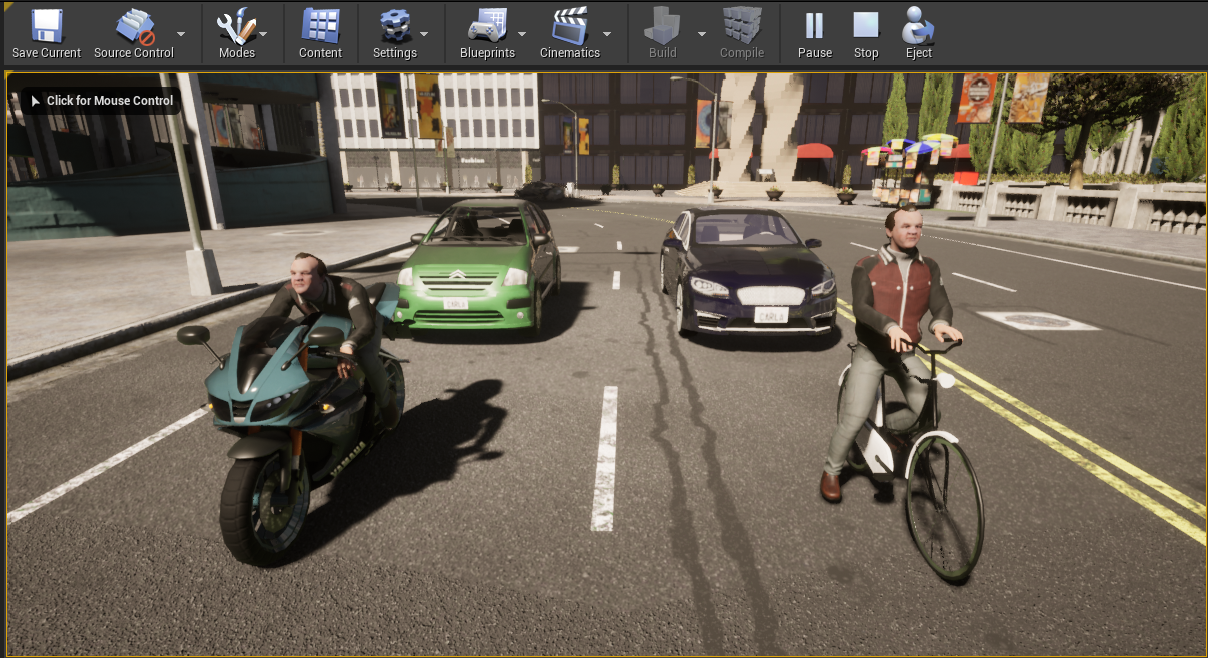
\includegraphics[width=\textwidth]{Figures/biker-cyclist.png}
\caption{CARLA simulator added actors}
\label{fig:biker-cyclist}
\end{figure}


%%%%%%%%%%%%%%%%%%%%%%%%%%%%%%%%%%%%%%%%%%%%%%%%%%%%%%%%%%%%%%%%%%%%%%%%%%%%%
% RUN 003 - Adding dynamic weather
%%%%%%%%%%%%%%%%%%%%%%%%%%%%%%%%%%%%%%%%%%%%%%%%%%%%%%%%%%%%%%%%%%%%%%%%%%%%%
\subsection{Run 003 - Adding dynamic weather}
\label{app_res:003}
\begin{verbatim}
Commit: bb4b95e0
Environment: Local desktop
Command:
$ make launch-only
# In another terminal, change directory to PythonAPI/examples, and run
$ python dynamic_weather.py -s 0.01
Sun(alt: -18.82, azm: 300.53) Storm(clouds=0%, rain=0%, wind=5%)            ^Z
[1]+  Stopped                 python3 dynamic_weather.py -s 0.01

Comment:
The parameter -s (speed) is a denominator in code, see
update_freq = 0.1 / speed_factor
The smaller the number, the less frequent (slower) are the weather updates, 
the greater the number, the more frequent (faster) are the weather updates.
\end{verbatim}

%%%%%%%%%%%%%%%%%%%%%%%%%%%%%%%%%%%%%%%%%%%%%%%%%%%%%%%%%%%%%%%%%%%%%%%%%%%%%
% RUN 004 - Automatic control
%%%%%%%%%%%%%%%%%%%%%%%%%%%%%%%%%%%%%%%%%%%%%%%%%%%%%%%%%%%%%%%%%%%%%%%%%%%%%
\subsection{Run 004 - Automatic control}
\label{app_res:004}
\begin{verbatim}
Commit: bb4b95e0
Environment: Local desktop
Date: 2021.11.21
Command:
$ make launch-only
# Once loaded, press play
# In another terminal, change directory to PythonAPI/examples, and run
$ python automatic_control.py

Comment:
This launches a pygame terminal, with a random vehicle set to ran
\end{verbatim}

%%%%%%%%%%%%%%%%%%%%%%%%%%%%%%%%%%%%%%%%%%%%%%%%%%%%%%%%%%%%%%%%%%%%%%%%%%%%%
% RUN 005 - Automatic control with traffic
%%%%%%%%%%%%%%%%%%%%%%%%%%%%%%%%%%%%%%%%%%%%%%%%%%%%%%%%%%%%%%%%%%%%%%%%%%%%%
\subsection{Run 005 - Automatic control with traffic}
\label{app_res:005}
\begin{verbatim}
Commit: bb4b95e0
Environment: Local desktop
Date: 2021.11.21
Command:
$ make launch-only
# Once loaded, press play
# In another terminal, change directory to PythonAPI/examples, and run
$ python generate_traffic.py 
spawned 30 vehicles and 10 walkers, press Ctrl+C to exit.

# In another terminal, change directory to PythonAPI/examples, and run
$ python automatic_control.py

Comment:
Traffic and automatic control vehicle are visible both in the pygame and unreal 
engine screens.
\end{verbatim}

%%%%%%%%%%%%%%%%%%%%%%%%%%%%%%%%%%%%%%%%%%%%%%%%%%%%%%%%%%%%%%%%%%%%%%%%%%%%%
% RUN 006 - Automatic control with traffic and dynamic weather
%%%%%%%%%%%%%%%%%%%%%%%%%%%%%%%%%%%%%%%%%%%%%%%%%%%%%%%%%%%%%%%%%%%%%%%%%%%%%
\subsection{Run 006- Automatic control with traffic and dynamic weather}
\label{app_res:006}
\begin{verbatim}
Commit: bb4b95e0
Environment: Local desktop
Date: 2021.11.21
Command:
$ make launch-only
# Once loaded, press play
# In another terminal, change directory to PythonAPI/examples, and run
$ python generate_traffic.py 
spawned 30 vehicles and 10 walkers, press Ctrl+C to exit.

# In another terminal, change directory to PythonAPI/examples, and run
$ python dynamic_weather.py -s 0.05
Sun(alt: -19.78, azm: 300.10) Storm(clouds=0%, rain=0%, wind=5%)  

# In another terminal, change directory to PythonAPI/examples, and run
$ python automatic_control.py

Comment:
The sun position changes every two seconds when parameter -s 0.05 is 
passed (0.1 / 0.05 = 2)

To exit the simulation:
1. Ensure dynamic_weather.py is not running or stop with CONTROL + C
2. Stop generate_traffic.py with CONTROL + C
3. Stop dynamic_weather.py with CONTROL + C
4. Stop Unreal Engine

If script generate_traffic.py is not stopped with CONTROL + C, and say CONTROL + Z, may still be running in the background. This will keep a lock on the port.

To list processes (open files) that have port 2000 open:
$ sudo lsof -t -i:2000
3281
3416

To check which process the process ID listed refers to:
$ ps aux | grep 3281
daniel    3281  0.9  0.2 1860476 90348 pts/1   Tl   17:25   0:29 python3 generate_traffic.py
daniel    7455  0.0  0.0  14432  1040 pts/1    S+   18:18   0:00 grep --color=auto 3281

To kill the process:
$ sudo kill -9 3281
[1]+  Killed                  python3 generate_traffic.py

\end{verbatim}

\begin{figure}[h!]
\centering
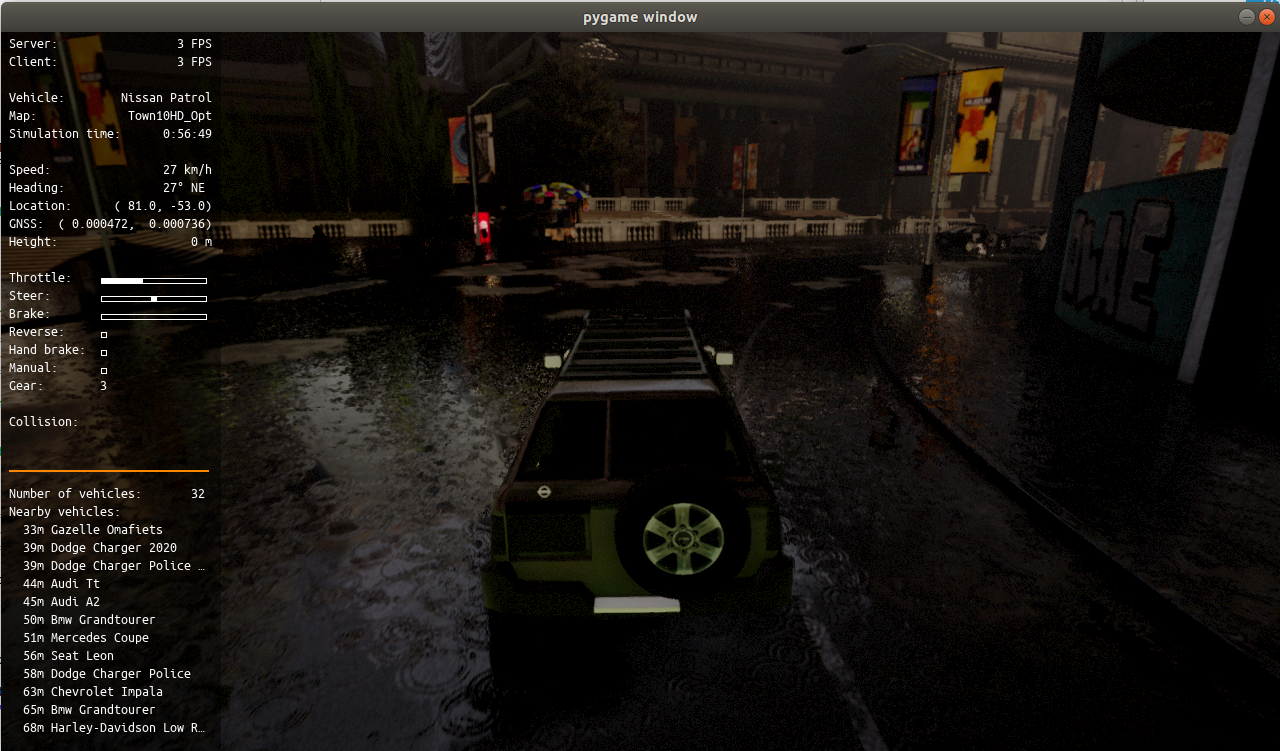
\includegraphics[width=\textwidth]{Figures/carla-rain.png}
\caption{CARLA simulator with dynamic weather}
\label{fig:carla-rain}
\end{figure}

\begin{figure}[h!]
\centering
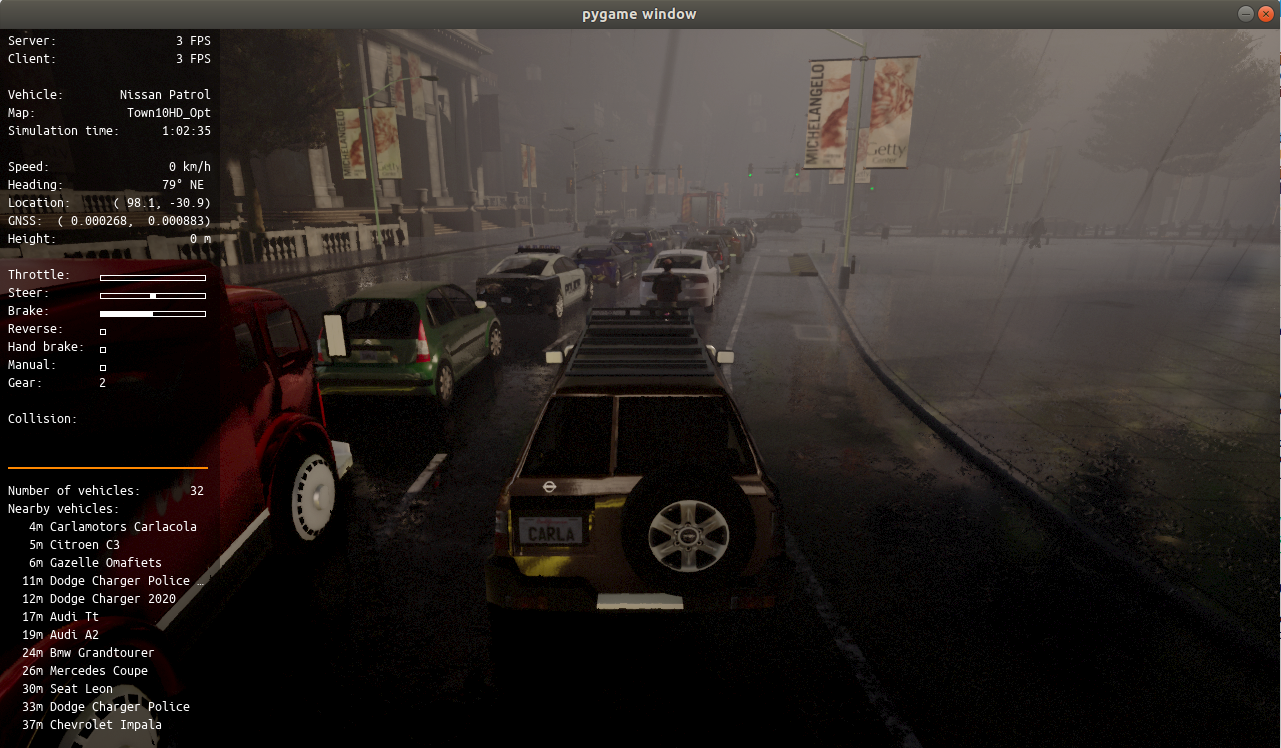
\includegraphics[width=\textwidth]{Figures/carla-traffic-jam.png}
\caption{CARLA simulator traffic jam}
\label{fig:carla-traffic-jam}
\end{figure}

Figures \ref{fig:carla-rain} and \ref{fig:carla-traffic-jam} are taken from the pygame screen.

\begin{figure}[h!]
\centering
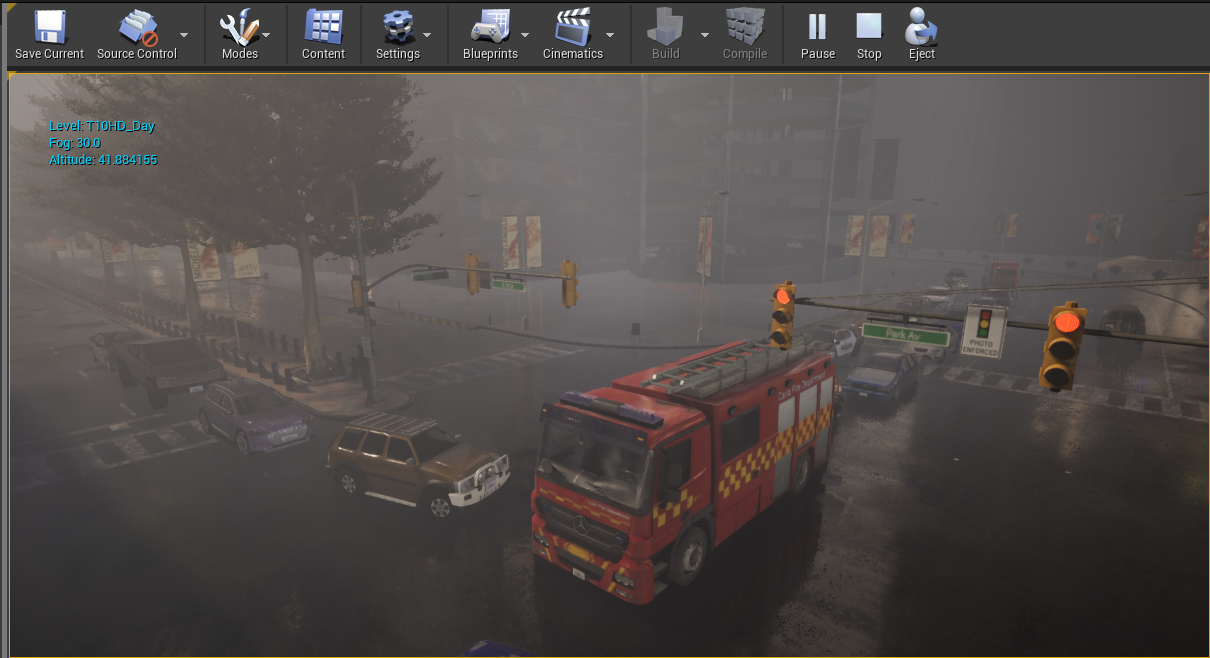
\includegraphics[width=\textwidth]{Figures/carla-traffic-jam-2.png}
\caption{CARLA simulator traffic jam reverse angle}
\label{fig:carla-traffic-jam-2}
\end{figure}

Figure \ref{fig:carla-traffic-jam-2}, taken from Unreal Engine, showing the stopped vehicles at the T-junction and is the reverse angle of Figure \ref{fig:carla-traffic-jam}. note there has not been a collision. The algorithm driving each vehicle seems to be stuck by a proximity assessment that is unlikely to change given all vehicles are stopped.

%%%%%%%%%%%%%%%%%%%%%%%%%%%%%%%%%%%%%%%%%%%%%%%%%%%%%%%%%%%%%%%%%%%%%%%%%%%%%
% RUN 007 - Automatic control with traffic
%%%%%%%%%%%%%%%%%%%%%%%%%%%%%%%%%%%%%%%%%%%%%%%%%%%%%%%%%%%%%%%%%%%%%%%%%%%%%
\subsection{Run 007- Automatic control with traffic}
\label{app_res:007}
\begin{verbatim}
Commit: bb4b95e0
Environment: Local desktop
Date: 2021.11.22
Commands:
$ make launch-only
# Loaded Town04_Opt
$ python generate_traffic.py -n 60 -w 600
spawned 60 vehicles and 328 walkers, press Ctrl+C to exit.
# NB some walkers not created due to collisions
# In another terminal, change directory to PythonAPI/examples, and run
$ python automatic_control.py

Comment:
Various successive runs, number of vehicles decreasing over time due to collisions. One simulated self-drving vehicle got stuck in the simulation (tipycally it would be destroyed at the end of self-driving simulation) after crashing against a traffic-light post.
\end{verbatim}

%%%%%%%%%%%%%%%%%%%%%%%%%%%%%%%%%%%%%%%%%%%%%%%%%%%%%%%%%%%%%%%%%%%%%%%%%%%%%
% RUN 008 - Using the same vehicle
%%%%%%%%%%%%%%%%%%%%%%%%%%%%%%%%%%%%%%%%%%%%%%%%%%%%%%%%%%%%%%%%%%%%%%%%%%%%%
\subsection{Run 008 - Using the same vehicle}
\label{app_res:008}
\begin{verbatim}
Commit: bb4b95e0
Environment: Local desktop
Date: 2021.12.05
Commands:
$ make launch-only
# Loaded Town10HD_Opt (current default)
# pressed "Play"
# generated dynamic weather
$ python dynamic_weather.py --speed 0.1
# generate traffic
$ python generate_traffic.py -n 60 -w 600
(...)
Vehicle agent not added to the crowd by some problem!
(...)
# error message assumed to caused by starting sequence i.e. dynamic weather before dynamic traffic.
$ python generate_traffic.py -n 60 -w 600

Comment:
Currently code uses a random vehicle chosen in automatic_control.py. All cars vanished from simulation two hours in. Pedestrians still present.
\end{verbatim}


%%%%%%%%%%%%%%%%%%%%%%%%%%%%%%%%%%%%%%%%%%%%%%%%%%%%%%%%%%%%%%%%%%%%%%%%%%%%%
% RUN 009 - Hyperion test
%%%%%%%%%%%%%%%%%%%%%%%%%%%%%%%%%%%%%%%%%%%%%%%%%%%%%%%%%%%%%%%%%%%%%%%%%%%%%
\subsection{Run 009 - Hyperion High Computing Cluster Test}
\label{app_res:009}
\begin{verbatim}

% Repository: https://github.com/dsikar/mscai
% Branch: master
% Commit: d4409a20
% Environment: Hyperion
% Date: 2022.03.20
% Connection details:
% As per "HPC - How to connect using windows"
% Commands:
% $ cd ~/localscratch 
% $ git clone https://github.com/dsikar/mscai
% $ cd Lab1
% # deactivate environment - activated by default in ~/.bashrc
% $ flight env deactivate
% # run
% $ source /opt/flight/etc/setup.sh
% $ flight env activate singularity
% $ singularity exec --nv /mnt/scratch/singularity/psarin/ubuntu20_04cuda11.sif   /usr/bin/python3 /users/aczd097/localscratch/mscai/Lab1/DLIALab1.py

% Comment:
% This script is supposed to run with 
% aczd097@login1 ~/localscratch/mscai/Lab1 (master)$ sbatch runModel.sh
% Submitted batch job 173522

% The JOBID does not appear in the queue. Assumption is job fails to start. Also, could be that access to gpu is currently restricted until end of term, as priority is for MScAI students.

% from: https://sylabs.io/guides/3.7/user-guide/definition_files.html
% The process of creating the singularity container (.sif file) is:

% 1. A script is created:
% /mnt/scratch/singularity/psarin/ubuntu20_04cuda11.def
% 2. And built:
% $ sudo singularity build --notest my_container.sif my_container.def

% # Proxy servers
% See: "HPC - Using the proxy server to install software from the internet"
% https://cityuni.service-now.com/sp?id=kb_article_view&sysparm_article=KB0012656

% # HPC - Environment modules
% Search HPC in Service Now

% # online help

% aczd097@login1 ~/fluent $ flight howto list

% | Index | Name                             |

% | 1     | Get Started                      |
% | 2     | Work With The Flight Environment |
% | 3     | Use Flight User Suite            |
% | 4     | Run Jobs                         |
% | 5     | Use A Scheduler                  |
% | 6     | Flight Desktop                   |
% | 7     | Flight Env                       |
% | 8     | Flight Job                       |

% aczd097@login1 ~/fluent $ flight howto show "Get Started"
% HOW TO GET STARTED(7)  Miscellaneous Information Manual  HOW TO GET STARTED(7)
% (...)

% <singularity{+}> [aczd097@login1 [hyperion] git]$ flight help env
%                                    __ _ _       _     _  ==>
%    ==>                            / _| (_)     | |   | |  ==>
%   ==>   ___   _ __    ___  _ __  | |_| |_  __ _| |__ | |_  ==>
%  ==>   / _ \ | '_ \  / _ \| '_ \ |  _| | |/ _` | '_ \| __|  ==>
% ==>   | (_) || |_) ||  __/| | | || | | | | (_| | | | | |_    ==>
%  ==>   \___/ | .__/  \___||_| |_||_| |_|_|\__, |_| |_|\__|  ==>
%   ==>        |_|                           __/ |           ==>
%    ==>  Flight Environment                |___/           ==>
%     ==>  v1.4.0

%   NAME:

%     flight env

%   DESCRIPTION:

%     Manage and access HPC application environments.

%   COMMANDS:

%     activate     Activate an application environment
%     avail        Show available application environment types
%     create       Create a new application environment
%     deactivate   Deactivate the current application environment
%     help         Display global or [command] help documentation
%     info         Show information about an application environment type
%     list         List configured application environments
%     purge        Purge an existing application environment
%     set-default  Set the default application environment
%     show-active  Show currently active application environment
%     show-default Show the default application environment
%     switch       Switch to a different application environment

% <singularity{+}> [aczd097@login1 [hyperion] git]$ flight env avail

% 
% | Name        | Summary                                                                                               |
%
% | brew        | The Missing Package Manager for macOS (or Linux)                                                      |
% |             |                                                                                                       |
% |             |  > https://brew.sh/                                                                                   |
% |             |                                                                                                       |
% | conda       | Package, dependency and environment management for any language.                                      |
% |             |                                                                                                       |
% |             |  > https://conda.io/                                                                                  |
% |             |                                                                                                       |
% | easybuild   | Software build and installation framework.                                                            |
% |             |                                                                                                       |
% |             |  > https://easybuilders.github.io/easybuild/                                                          |
% |             |                                                                                                       |
% | gridware    | Tool for installing and managing scientific applications and libraries.                               |
% |             |                                                                                                       |
% |             |  > https://gridware.alces-flight.com/                                                                 |
% |             |                                                                                                       |
% | modules     | Provides dynamic modification of a user's environment.                                                |
% |             |                                                                                                       |
% |             |  > http://modules.sourceforge.net/                                                                    |
% |             |                                                                                                       |
% | singularity | Container solution for scientific and application driven workloads.                                   |
% |             |                                                                                                       |
% |             |  > https://www.sylabs.io/                                                                             |
% |             |                                                                                                       |
% | spack       | A flexible package manager that supports multiple versions, configurations, platforms, and compilers. |
% |             |  > https://spack.io/                                                                                  |
% |             |                                                                                                       |


\end{verbatim}


%%%%%%%%%%%%%%%%%%%%%%%%%%%%%%%%%%%%%%%%%%%%%%%%%%%%%%%%%%%%%%%%%%%%%%%%%%%%%
% RUN 010 - Dynamic weather
%%%%%%%%%%%%%%%%%%%%%%%%%%%%%%%%%%%%%%%%%%%%%%%%%%%%%%%%%%%%%%%%%%%%%%%%%%%%%
\subsection{Run 010 - Dynamic Weather}
\label{app_res:010}
\begin{verbatim}

Commit: bb4b95e0
Environment: Local desktop
Date: 2021.12.05
Commands:
$ make launch-only
# Loaded Town10HD_Opt (current default)
# pressed "Play"
# generated dynamic weather
$ python dynamic_weather.py --speed 0.1
# generate traffic
$ python generate_traffic.py -n 60 -w 600
(...)
Vehicle agent not added to the crowd by some problem!
(...)
# error message assumed to caused by starting sequence i.e. dynamic weather before dynamic traffic.
$ python generate_traffic.py -n 60 -w 600

Comment:
Currently code uses a random vehicle chosen in automatic_control.py. All cars vanished from simulation two hours in. Pedestrians still present.

\end{verbatim}

%%%%%%%%%%%%%%%%%%%%%%%%%%%%%%%%%%%%%%%%%%%%%%%%%%%%%%%%%%%%%%%%%%%%%%%%%%%%%
% RUN 010 - CIFAR10 Vanilla CNN
%%%%%%%%%%%%%%%%%%%%%%%%%%%%%%%%%%%%%%%%%%%%%%%%%%%%%%%%%%%%%%%%%%%%%%%%%%%%%
\subsection{Run 010 - CIFAR10 Vanilla CNN}
\label{app_res:010}
\begin{verbatim}
Repository: https://github.com/dsikar/quant
Commit: aae016eab3
Environment: Local GPU
Date: 2023.07.23
Commands: python vanilla_cnn_quant.py

\end{verbatim}


%%%%%%%%%%%%%%%%%%%%%%%%%%%%%%%%%%%%%%%%%%%%%%%%%%%%%%%%%%%%%%%%%%%%%%%%%%%%%
% RUN 011 - Contrast test
%%%%%%%%%%%%%%%%%%%%%%%%%%%%%%%%%%%%%%%%%%%%%%%%%%%%%%%%%%%%%%%%%%%%%%%%%%%%%
\subsection{Run 011- Contrast test}
\label{app_res:011}
\begin{verbatim}
Repository: git@github.com:dsikar/ecai2023
Commit: 62fbc1a
Environment: Local GPU
Date: 2023.10.15
Commands: python unit-tests.py
\end{verbatim}

Note, the number of bins used here was 21.

\begin{figure}[h]
\begin{center}
%\framebox[4.0in]{$\;$}
%\fbox{\rule[-.5cm]{0cm}{4cm} \rule[-.5cm]{4cm}{0cm}}
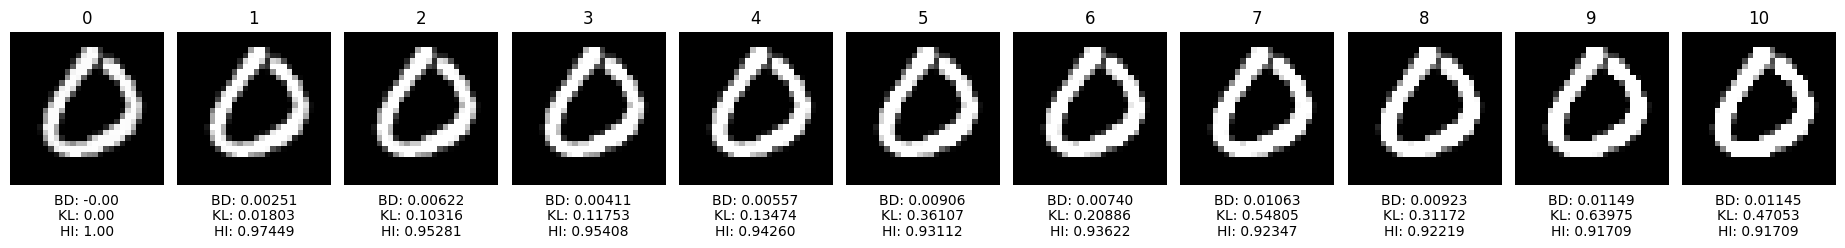
\includegraphics[width=\textwidth]{Figures/Appendixes/brightenss_perturbations_21_bins_27d2880.png}
\end{center}
\caption{Modifying brightness for an MNIST image of the number 0, using 21 bins.}
\end{figure}

%%%%%%%%%%%%%%%%%%%%%%%%%%%%%%%%%%%%%%%%%%%%%%%%%%%%%%%%%%%%%%%%%%%%%%%%%%%%%
% RUN 012 - Contrast test
%%%%%%%%%%%%%%%%%%%%%%%%%%%%%%%%%%%%%%%%%%%%%%%%%%%%%%%%%%%%%%%%%%%%%%%%%%%%%
\subsection{Run 012- Contrast test}
\label{app_res:012}
\begin{verbatim}
Repository: git@github.com:dsikar/ecai2023
Commit: 2c7ca28
Environment: Local GPU
Date: 2023.10.15
Commands: python unit-tests.py
\end{verbatim}

Note, the number of bins used here was 30.

\begin{figure}[h]
\begin{center}
%\framebox[4.0in]{$\;$}
%\fbox{\rule[-.5cm]{0cm}{4cm} \rule[-.5cm]{4cm}{0cm}}
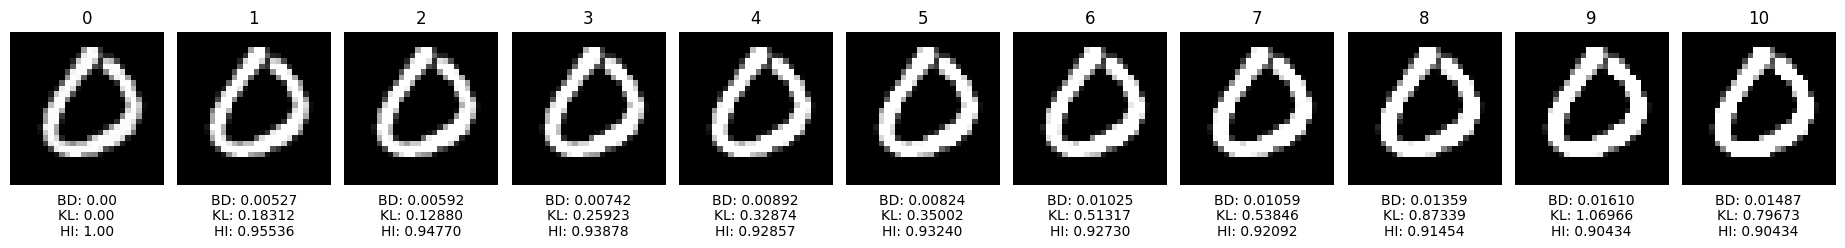
\includegraphics[width=\textwidth]{Figures/Appendixes/brightness_perturbations_30_bins.png}
\end{center}
\caption{Modifying brightness for an MNIST image of the number 0, using 30 bins.}
\end{figure}


%%%%%%%%%%%%%%%%%%%%%%%%%%%%%%%%%%%%%%%%%%%%%%%%%%%%%%%%%%%%%%%%%%%%%%%%%%%%%
% RUN 013 - MNIST Preliminary results
%%%%%%%%%%%%%%%%%%%%%%%%%%%%%%%%%%%%%%%%%%%%%%%%%%%%%%%%%%%%%%%%%%%%%%%%%%%%%
\subsection{Run 013- MNIST preliminary results}
\label{app_res:013}
\begin{verbatim}
Repository: git@github.com:dsikar/ecai2023
Commit: ca91409
Environment: Local GPU
Date: 2023.10.29
Commands: python mnist_cnn_generate_tables.py
\end{verbatim}

Some preliminary data, stored results in scripts/data. Note, need to work on the perturbation levels, to try to match the accuracy to noise levels across all perturbation types.

%%%%%%%%%%%%%%%%%%%%%%%%%%%%%%%%%%%%%%%%%%%%%%%%%%%%%%%%%%%%%%%%%%%%%%%%%%%%%
% RUN 014 - MNIST Preliminary results changed contrast
%%%%%%%%%%%%%%%%%%%%%%%%%%%%%%%%%%%%%%%%%%%%%%%%%%%%%%%%%%%%%%%%%%%%%%%%%%%%%
\subsection{Run 014- MNIST evaluating constrast levels}
\label{app_res:014}
\begin{verbatim}
Repository: git@github.com:dsikar/work-in-progress
Commit: 95be2d0
Environment: Local GPU
Date: 2023.11.19
Commands: python mnist_cnn_eval.py
\end{verbatim}

Modifying the ordering in contrast levels, such that accuracy will decrease as perturbation level increases.

Note, repository name changed from git@github.com:dsikar/ecai2023 to git@github.com:dsikar/work-in-progress.

% Accuracy: 95.8300, with perturbation type contrast values = {'contrast_level': 2.9}, Bhattacharyya Distance: 0.0234, KL Divergence: 1.7614, Histogram Intersection: 0.9053
% Accuracy: 95.5800, with perturbation type contrast values = {'contrast_level': 2.8}, Bhattacharyya Distance: 0.0233, KL Divergence: 1.7473, Histogram Intersection: 0.9056
% Accuracy: 95.1400, with perturbation type contrast values = {'contrast_level': 2.7}, Bhattacharyya Distance: 0.0232, KL Divergence: 1.7322, Histogram Intersection: 0.9058
% Accuracy: 94.8900, with perturbation type contrast values = {'contrast_level': 2.6}, Bhattacharyya Distance: 0.0231, KL Divergence: 1.7221, Histogram Intersection: 0.9061
% Accuracy: 94.4500, with perturbation type contrast values = {'contrast_level': 2.5}, Bhattacharyya Distance: 0.0230, KL Divergence: 1.7080, Histogram Intersection: 0.9063
% Accuracy: 94.0300, with perturbation type contrast values = {'contrast_level': 2.4}, Bhattacharyya Distance: 0.0229, KL Divergence: 1.6932, Histogram Intersection: 0.9066
% Accuracy: 93.5400, with perturbation type contrast values = {'contrast_level': 2.3}, Bhattacharyya Distance: 0.0228, KL Divergence: 1.6782, Histogram Intersection: 0.9070
% Accuracy: 93.0300, with perturbation type contrast values = {'contrast_level': 2.2}, Bhattacharyya Distance: 0.0226, KL Divergence: 1.6614, Histogram Intersection: 0.9073
% Accuracy: 92.4100, with perturbation type contrast values = {'contrast_level': 2.1}, Bhattacharyya Distance: 0.0225, KL Divergence: 1.6498, Histogram Intersection: 0.9075
% Accuracy: 91.7900, with perturbation type contrast values = {'contrast_level': 2.0}, Bhattacharyya Distance: 0.0224, KL Divergence: 1.6375, Histogram Intersection: 0.9078
% Accuracy: 91.0100, with perturbation type contrast values = {'contrast_level': 1.9}, Bhattacharyya Distance: 0.0223, KL Divergence: 1.6164, Histogram Intersection: 0.9082
% Accuracy: 90.2900, with perturbation type contrast values = {'contrast_level': 1.8}, Bhattacharyya Distance: 0.0221, KL Divergence: 1.6051, Histogram Intersection: 0.9086
% Accuracy: 89.4800, with perturbation type contrast values = {'contrast_level': 1.7}, Bhattacharyya Distance: 0.0219, KL Divergence: 1.5845, Histogram Intersection: 0.9090
% Accuracy: 88.7600, with perturbation type contrast values = {'contrast_level': 1.6}, Bhattacharyya Distance: 0.0218, KL Divergence: 1.5692, Histogram Intersection: 0.9094
% Accuracy: 87.8000, with perturbation type contrast values = {'contrast_level': 1.5}, Bhattacharyya Distance: 0.0217, KL Divergence: 1.5511, Histogram Intersection: 0.9098
% Accuracy: 87.0500, with perturbation type contrast values = {'contrast_level': 1.4}, Bhattacharyya Distance: 0.0215, KL Divergence: 1.5365, Histogram Intersection: 0.9102
% Accuracy: 86.5100, with perturbation type contrast values = {'contrast_level': 1.3}, Bhattacharyya Distance: 0.0214, KL Divergence: 1.5199, Histogram Intersection: 0.9107
% Accuracy: 85.9600, with perturbation type contrast values = {'contrast_level': 1.2}, Bhattacharyya Distance: 0.0212, KL Divergence: 1.4996, Histogram Intersection: 0.9113
% Accuracy: 85.4700, with perturbation type contrast values = {'contrast_level': 1.1}, Bhattacharyya Distance: 0.0210, KL Divergence: 1.4771, Histogram Intersection: 0.9119
% Accuracy: 85.0700, with perturbation type contrast values = {'contrast_level': 1.0}, Bhattacharyya Distance: 0.0208, KL Divergence: 1.4600, Histogram Intersection: 0.9125
% Accuracy: 84.3400, with perturbation type contrast values = {'contrast_level': 0.9}, Bhattacharyya Distance: 0.0207, KL Divergence: 1.4402, Histogram Intersection: 0.9131
% Accuracy: 83.9800, with perturbation type contrast values = {'contrast_level': 0.8}, Bhattacharyya Distance: 0.0205, KL Divergence: 1.4202, Histogram Intersection: 0.9139
% Accuracy: 83.5500, with perturbation type contrast values = {'contrast_level': 0.7}, Bhattacharyya Distance: 0.0203, KL Divergence: 1.3963, Histogram Intersection: 0.9147
% Accuracy: 83.0200, with perturbation type contrast values = {'contrast_level': 0.6}, Bhattacharyya Distance: 0.0200, KL Divergence: 1.3659, Histogram Intersection: 0.9157
% Accuracy: 82.4400, with perturbation type contrast values = {'contrast_level': 0.5}, Bhattacharyya Distance: 0.0197, KL Divergence: 1.3381, Histogram Intersection: 0.9167
% Accuracy: 81.8100, with perturbation type contrast values = {'contrast_level': 0.4}, Bhattacharyya Distance: 0.0195, KL Divergence: 1.3016, Histogram Intersection: 0.9178
% Accuracy: 81.0200, with perturbation type contrast values = {'contrast_level': 0.3}, Bhattacharyya Distance: 0.0192, KL Divergence: 1.2624, Histogram Intersection: 0.9191
% Accuracy: 80.0600, with perturbation type contrast values = {'contrast_level': 0.2}, Bhattacharyya Distance: 0.0188, KL Divergence: 1.2234, Histogram Intersection: 0.9206
% Accuracy: 79.1800, with perturbation type contrast values = {'contrast_level': 0.1}, Bhattacharyya Distance: 0.0184, KL Divergence: 1.1720, Histogram Intersection: 0.9224
% Accuracy: 84.3400, with perturbation type contrast values = {'contrast_level': 0.9}, Bhattacharyya Distance: 0.0207, KL Divergence: 1.4402, Histogram Intersection: 0.9131
% Accuracy: 83.9800, with perturbation type contrast values = {'contrast_level': 0.8}, Bhattacharyya Distance: 0.0205, KL Divergence: 1.4202, Histogram Intersection: 0.9139
% Accuracy: 83.5500, with perturbation type contrast values = {'contrast_level': 0.7}, Bhattacharyya Distance: 0.0203, KL Divergence: 1.3963, Histogram Intersection: 0.9147
% Accuracy: 83.0200, with perturbation type contrast values = {'contrast_level': 0.6}, Bhattacharyya Distance: 0.0200, KL Divergence: 1.3659, Histogram Intersection: 0.9157
% Accuracy: 82.4400, with perturbation type contrast values = {'contrast_level': 0.5}, Bhattacharyya Distance: 0.0197, KL Divergence: 1.3381, Histogram Intersection: 0.9167
% Accuracy: 81.8100, with perturbation type contrast values = {'contrast_level': 0.4}, Bhattacharyya Distance: 0.0195, KL Divergence: 1.3016, Histogram Intersection: 0.9178
% Accuracy: 81.0200, with perturbation type contrast values = {'contrast_level': 0.3}, Bhattacharyya Distance: 0.0192, KL Divergence: 1.2624, Histogram Intersection: 0.9191
% Accuracy: 80.0600, with perturbation type contrast values = {'contrast_level': 0.2}, Bhattacharyya Distance: 0.0188, KL Divergence: 1.2234, Histogram Intersection: 0.9206
% Accuracy: 79.1800, with perturbation type contrast values = {'contrast_level': 0.1}, Bhattacharyya Distance: 0.0184, KL Divergence: 1.1720, Histogram Intersection: 0.9224
% Accuracy: 78.3400, with perturbation type contrast values = {'contrast_level': 0.0}, Bhattacharyya Distance: 0.0179, KL Divergence: 1.1160, Histogram Intersection: 0.9247
% Accuracy: 77.0800, with perturbation type contrast values = {'contrast_level': -0.1}, Bhattacharyya Distance: 0.0174, KL Divergence: 1.0530, Histogram Intersection: 0.9272
% Accuracy: 75.2700, with perturbation type contrast values = {'contrast_level': -0.2}, Bhattacharyya Distance: 0.0169, KL Divergence: 0.9794, Histogram Intersection: 0.9306
% Accuracy: 73.4300, with perturbation type contrast values = {'contrast_level': -0.3}, Bhattacharyya Distance: 0.0158, KL Divergence: 0.8528, Histogram Intersection: 0.9369
% Accuracy: 70.9200, with perturbation type contrast values = {'contrast_level': -0.4}, Bhattacharyya Distance: 0.0089, KL Divergence: 0.4424, Histogram Intersection: 0.9652
% Accuracy: 65.2400, with perturbation type contrast values = {'contrast_level': -0.5}, Bhattacharyya Distance: 0.0001, KL Divergence: 0.0018, Histogram Intersection: 0.9997
% Accuracy: 54.8700, with perturbation type contrast values = {'contrast_level': -0.6}, Bhattacharyya Distance: 0.0001, KL Divergence: 0.0039, Histogram Intersection: 0.9994
% Accuracy: 38.7700, with perturbation type contrast values = {'contrast_level': -0.7}, Bhattacharyya Distance: 0.0001, KL Divergence: 0.0031, Histogram Intersection: 0.9995
% Accuracy: 16.6700, with perturbation type contrast values = {'contrast_level': -0.8}, Bhattacharyya Distance: 0.0001, KL Divergence: 0.0025, Histogram Intersection: 0.9995
% Accuracy: 9.7400, with perturbation type contrast values = {'contrast_level': -0.9}, Bhattacharyya Distance: 0.0001, KL Divergence: 0.0030, Histogram Intersection: 0.9994
% Accuracy: 9.7400, with perturbation type contrast values = {'contrast_level': -1.0}, Bhattacharyya Distance: -1.3617, KL Divergence: 28.6177, Histogram Intersection: 0.0033

%%%%%%%%%%%%%%%%%%%%%%%%%%%%%%%%%%%%%%%%%%%%%%%%%%%%%%%%%%%%%%%%%%%%%%%%%%%%%
% RUN 015 - MNIST Contrast Levels
%%%%%%%%%%%%%%%%%%%%%%%%%%%%%%%%%%%%%%%%%%%%%%%%%%%%%%%%%%%%%%%%%%%%%%%%%%%%%
\subsection{Run 015 - MNIST contrast level plots}
\label{app_res:015}
\begin{verbatim}
Repository: git@github.com:dsikar/work-in-progress
Commit: 5399d69
Environment: Local GPU
Date: 2023.11.26
Commands: python contrast_levels.py
\end{verbatim}

\begin{table}[ht]
\centering
\begin{tabular}{|c|c|c|c|c|}
\hline
Contrast Level & Accuracy & BD & KL & HI \\
\hline
3.0 & 96.0000 & 0.0235 & 1.7749 & 0.9050 \\
2.9 & 95.8300 & 0.0234 & 1.7614 & 0.9053 \\
2.8 & 95.5800 & 0.0233 & 1.7473 & 0.9056 \\
2.7 & 95.1400 & 0.0232 & 1.7322 & 0.9058 \\
2.6 & 94.8900 & 0.0231 & 1.7221 & 0.9061 \\
2.5 & 94.4500 & 0.0230 & 1.7080 & 0.9063 \\
2.4 & 94.0300 & 0.0229 & 1.6932 & 0.9066 \\
2.3 & 93.5400 & 0.0228 & 1.6782 & 0.9070 \\
2.2 & 93.0300 & 0.0226 & 1.6614 & 0.9073 \\
2.1 & 92.4100 & 0.0225 & 1.6498 & 0.9075 \\
2.0 & 91.7900 & 0.0224 & 1.6375 & 0.9078 \\
1.9 & 91.0100 & 0.0223 & 1.6164 & 0.9082 \\
1.8 & 90.2900 & 0.0221 & 1.6051 & 0.9086 \\
1.7 & 89.4800 & 0.0219 & 1.5845 & 0.9090 \\
1.6 & 88.7600 & 0.0218 & 1.5692 & 0.9094 \\
1.5 & 87.8000 & 0.0217 & 1.5511 & 0.9098 \\
1.4 & 87.0500 & 0.0215 & 1.5365 & 0.9102 \\
1.3 & 86.5100 & 0.0214 & 1.5199 & 0.9107 \\
1.2 & 85.9600 & 0.0212 & 1.4996 & 0.9113 \\
1.1 & 85.4700 & 0.0210 & 1.4771 & 0.9119 \\
1.0 & 85.0700 & 0.0208 & 1.4600 & 0.9125 \\
0.9 & 84.3400 & 0.0207 & 1.4402 & 0.9131 \\
0.8 & 83.9800 & 0.0205 & 1.4202 & 0.9139 \\
0.7 & 83.5500 & 0.0203 & 1.3963 & 0.9147 \\
0.6 & 83.0200 & 0.0200 & 1.3659 & 0.9157 \\
0.5 & 82.4400 & 0.0197 & 1.3381 & 0.9167 \\
0.4 & 81.8100 & 0.0195 & 1.3016 & 0.9178 \\
0.3 & 81.0200 & 0.0192 & 1.2624 & 0.9191 \\
0.2 & 80.0600 & 0.0188 & 1.2234 & 0.9206 \\
0.0 & 78.3400 & 0.0179 & 1.1160 & 0.9247 \\
-0.1 & 77.0800 & 0.0174 & 1.0530 & 0.9272 \\
-0.2 & 75.2700 & 0.0169 & 0.9794 & 0.9306 \\
-0.3 & 73.4300 & 0.0158 & 0.8528 & 0.9369 \\
-0.4 & 70.9200 & 0.0089 & 0.4424 & 0.9652 \\
-0.5 & 65.2400 & 0.0001 & 0.0018 & 0.9997 \\
-0.6 & 54.8700 & 0.0001 & 0.0039 & 0.9994 \\
-0.7 & 38.7700 & 0.0001 & 0.0031 & 0.9995 \\
-0.8 & 16.6700 & 0.0001 & 0.0025 & 0.9995 \\
-0.9 & 9.7400 & 0.0001 & 0.0030 & 0.9994 \\
-1.0 & 9.7400 & -1.3617 & 28.6177 & 0.0033 \\

\hline
\end{tabular}
\caption{Experimental contrast levels and resulting Accuracy, Bhatacharya Distance (BD), KL Divergence (KL) and Histogram Intersection (HI) for contrast applied to MNIST testing dataset and resulting accuracy and distance metrics, where accuracy on original testing MNIST Dataset is 98.38\%}
\label{your-label-here}
\end{table}

%%%%%%%%%%%%%%%%%%%%%%%%%%%%%%%%%%%%%%%%%%%%%%%%%%%%%%%%%%%%%%%%%%%%%%%%%%%%%
% RUN 016 - MNIST Brightness Levels
%%%%%%%%%%%%%%%%%%%%%%%%%%%%%%%%%%%%%%%%%%%%%%%%%%%%%%%%%%%%%%%%%%%%%%%%%%%%%
\subsection{Run 016 - MNIST brightness level plot and table}
\label{app_res:016}
\begin{verbatim}
Repository: git@github.com:dsikar/work-in-progress
Commit: 20d96b36
Environment: Local GPU
Date: 2023.12.16
Commands: python contrast_levels.py # edited for brightness
\end{verbatim}

%%%%%%%%%%%%%%%%%%%%%%%%%%%%%%%%%%%%%%%%%%%%%%%%%%%%%%%%%%%%%%%%%%%%%%%%%%%%%
% RUN 017 - MNIST Defocus Blur Levels
%%%%%%%%%%%%%%%%%%%%%%%%%%%%%%%%%%%%%%%%%%%%%%%%%%%%%%%%%%%%%%%%%%%%%%%%%%%%%
\subsection{Run 017 - MNIST defocus level plot and table}
\label{app_res:017}
\begin{verbatim}
Repository: git@github.com:dsikar/work-in-progress
Commit: ee06742
Environment: Local GPU
Date: 2023.12.16
Commands: python mnist_cnn_eval.py 
\end{verbatim}

Results commented out in latex. 

% Accuracy on test dataset: 98.38%
% Perturbation type: defocus_blur
% Accuracy: 98.4000, with perturbation type defocus_blur values = {'kernel_size': 3, 'blur_amount': 0.1}, Bhattacharyya Distance: 0.0168, KL Divergence: 0.3240, Histogram Intersection: 0.9051
% Accuracy: 98.3100, with perturbation type defocus_blur values = {'kernel_size': 3, 'blur_amount': 0.2}, Bhattacharyya Distance: 0.0282, KL Divergence: 0.4355, Histogram Intersection: 0.8472
% Accuracy: 98.2300, with perturbation type defocus_blur values = {'kernel_size': 3, 'blur_amount': 0.3}, Bhattacharyya Distance: 0.0316, KL Divergence: 0.4353, Histogram Intersection: 0.8291
% Accuracy: 98.0300, with perturbation type defocus_blur values = {'kernel_size': 3, 'blur_amount': 0.4}, Bhattacharyya Distance: 0.0334, KL Divergence: 0.4271, Histogram Intersection: 0.8201
% Accuracy: 97.9900, with perturbation type defocus_blur values = {'kernel_size': 3, 'blur_amount': 0.5}, Bhattacharyya Distance: 0.0342, KL Divergence: 0.4022, Histogram Intersection: 0.8156
% Accuracy: 97.7700, with perturbation type defocus_blur values = {'kernel_size': 3, 'blur_amount': 0.6}, Bhattacharyya Distance: 0.0348, KL Divergence: 0.3769, Histogram Intersection: 0.8125
% Accuracy: 97.4800, with perturbation type defocus_blur values = {'kernel_size': 3, 'blur_amount': 0.7}, Bhattacharyya Distance: 0.0354, KL Divergence: 0.3671, Histogram Intersection: 0.8101
% Accuracy: 97.1500, with perturbation type defocus_blur values = {'kernel_size': 3, 'blur_amount': 0.8}, Bhattacharyya Distance: 0.0365, KL Divergence: 0.3710, Histogram Intersection: 0.8069
% Accuracy: 96.7400, with perturbation type defocus_blur values = {'kernel_size': 3, 'blur_amount': 0.9}, Bhattacharyya Distance: 0.0371, KL Divergence: 0.3773, Histogram Intersection: 0.8049
% Accuracy: 96.1100, with perturbation type defocus_blur values = {'kernel_size': 3, 'blur_amount': 1.0}, Bhattacharyya Distance: 0.0377, KL Divergence: 0.3916, Histogram Intersection: 0.8028
% Accuracy: 83.1900, with perturbation type defocus_blur values = {'kernel_size': 5, 'blur_amount': 1.1}, Bhattacharyya Distance: 0.0633, KL Divergence: 0.6136, Histogram Intersection: 0.6863
% Accuracy: 83.4100, with perturbation type defocus_blur values = {'kernel_size': 5, 'blur_amount': 1.2}, Bhattacharyya Distance: 0.0653, KL Divergence: 0.6819, Histogram Intersection: 0.6823
% Accuracy: 84.9200, with perturbation type defocus_blur values = {'kernel_size': 5, 'blur_amount': 1.3}, Bhattacharyya Distance: 0.0670, KL Divergence: 0.7545, Histogram Intersection: 0.6790
% Accuracy: 87.2600, with perturbation type defocus_blur values = {'kernel_size': 5, 'blur_amount': 1.4}, Bhattacharyya Distance: 0.0679, KL Divergence: 0.8066, Histogram Intersection: 0.6774
% Accuracy: 89.2900, with perturbation type defocus_blur values = {'kernel_size': 5, 'blur_amount': 1.5}, Bhattacharyya Distance: 0.0681, KL Divergence: 0.8386, Histogram Intersection: 0.6776
% Accuracy: 90.8200, with perturbation type defocus_blur values = {'kernel_size': 5, 'blur_amount': 1.6}, Bhattacharyya Distance: 0.0675, KL Divergence: 0.8443, Histogram Intersection: 0.6801
% Accuracy: 91.5500, with perturbation type defocus_blur values = {'kernel_size': 5, 'blur_amount': 1.7}, Bhattacharyya Distance: 0.0660, KL Divergence: 0.8252, Histogram Intersection: 0.6847
% Accuracy: 91.4300, with perturbation type defocus_blur values = {'kernel_size': 5, 'blur_amount': 1.8}, Bhattacharyya Distance: 0.0638, KL Divergence: 0.7882, Histogram Intersection: 0.6910
% Accuracy: 90.8100, with perturbation type defocus_blur values = {'kernel_size': 5, 'blur_amount': 1.9}, Bhattacharyya Distance: 0.0611, KL Divergence: 0.7381, Histogram Intersection: 0.6989
% Accuracy: 89.9400, with perturbation type defocus_blur values = {'kernel_size': 5, 'blur_amount': 2.0}, Bhattacharyya Distance: 0.0586, KL Divergence: 0.6823, Histogram Intersection: 0.7065
% Saved to file: vanilla_cnn_mnist_20231217172454.pkl



%%%%%%%%%%%%%%%%%%%%%%%%%%%%%%%%%%%%%%%%%%%%%%%%%%%%%%%%%%%%%%%%%%%%%%%%%%%%%
% RUN 018 - MNIST Fog Levels
%%%%%%%%%%%%%%%%%%%%%%%%%%%%%%%%%%%%%%%%%%%%%%%%%%%%%%%%%%%%%%%%%%%%%%%%%%%%%
\subsection{Run 018 - MNIST fog plot and table}
\label{app_res:018}
\begin{verbatim}
Repository: git@github.com:dsikar/work-in-progress
Commit: e1bea3c
Environment: Local GPU
Date: 2023.12.16
Commands: python mnist_cnn_eval.py 
\end{verbatim}

Added fog levels to work-in-progress.

%%%%%%%%%%%%%%%%%%%%%%%%%%%%%%%%%%%%%%%%%%%%%%%%%%%%%%%%%%%%%%%%%%%%%%%%%%%%%
% RUN 019 - MNIST Gaussian Noise Levels
%%%%%%%%%%%%%%%%%%%%%%%%%%%%%%%%%%%%%%%%%%%%%%%%%%%%%%%%%%%%%%%%%%%%%%%%%%%%%
\subsection{Run 019 - MNIST Gaussian Noise plot and table}
\label{app_res:019}
\begin{verbatim}
Repository: git@github.com:dsikar/work-in-progress
Commit: 0673368
Environment: Local GPU
Date: 2023.12.23
Commands: python gaussian_noise_levels.py 
\end{verbatim}

Added Gaussian levels to work-in-progress.

\begin{table}[ht]
\centering
\begin{tabular}{|c|c|c|c|c|}
\hline
Gaussian Noise Level & Accuracy & BD & KL & HI \\
\hline
1.00 & 98.3300 & 0.0948 & 0.7330 & 0.5408 \\
2.00 & 93.5300 & 0.3278 & 2.5286 & 0.2032 \\
3.00 & 85.9200 & 0.3922 & 3.2614 & 0.1798 \\
4.00 & 80.4900 & 0.4215 & 3.6819 & 0.1733 \\
5.00 & 76.1400 & 0.4476 & 4.1378 & 0.1685 \\
6.00 & 71.5200 & 0.4676 & 4.5594 & 0.1652 \\
7.00 & 66.7400 & 0.4797 & 4.8580 & 0.1632 \\
8.00 & 60.5600 & 0.4849 & 5.0233 & 0.1621 \\
9.00 & 56.0000 & 0.4862 & 5.0806 & 0.1618 \\
10.00 & 50.5300 & 0.4863 & 5.1120 & 0.1616 \\
\hline
\end{tabular}
\caption{Experimental Gaussian noise levels and resulting Accuracy, Bhattacharya Distance (BD), KL Divergence (KL) and Histogram Intersection (HI) for noise applied to MNIST testing dataset and resulting accuracy and distance metrics, where accuracy on original testing MNIST Dataset is 98.38\%}
\label{tbl-fog-levels}
\end{table}

%%%%%%%%%%%%%%%%%%%%%%%%%%%%%%%%%%%%%%%%%%%%%%%%%%%%%%%%%%%%%%%%%%%%%%%%%%%%%
% RUN 020 - MNIST Impulse Noise Levels
%%%%%%%%%%%%%%%%%%%%%%%%%%%%%%%%%%%%%%%%%%%%%%%%%%%%%%%%%%%%%%%%%%%%%%%%%%%%%
\subsection{Run 020 - MNIST Impulse Noise plot and table}
\label{app_res:020}
\begin{verbatim}
Repository: git@github.com:dsikar/work-in-progress
Commit: c755432
Environment: Local GPU
Date: 2023.12.23
Commands:python noise_levels.py "impulse_noise" "Impulse Noise" \
"vanilla_cnn_mnist_20231223171844_impulse_noise.pkl"
\end{verbatim}

\begin{table}[ht]
\centering
\begin{tabular}{|c|c|c|c|c|}
\hline
Gaussian Noise Level & Accuracy & BD & KL & HI \\
\hline
1.00 & 94.8600 & 0.0448 & 0.3418 & 0.7733 \\
2.00 & 88.1200 & 0.0684 & 0.5230 & 0.6844 \\
3.00 & 82.1100 & 0.0817 & 0.6260 & 0.6400 \\
4.00 & 76.9000 & 0.0961 & 0.7402 & 0.5956 \\
5.00 & 71.7200 & 0.1122 & 0.8708 & 0.5501 \\
6.00 & 67.4400 & 0.1295 & 1.0114 & 0.5059 \\
7.00 & 62.9400 & 0.1487 & 1.1693 & 0.4616 \\
8.00 & 58.2700 & 0.1702 & 1.3549 & 0.4175 \\
9.00 & 53.9600 & 0.1948 & 1.5666 & 0.3732 \\
10.00 & 49.8400 & 0.2239 & 1.8144 & 0.3280 \\
\hline
\end{tabular}
\caption{Experimental Impulse noise levels and resulting Accuracy, Bhattacharya Distance (BD), KL Divergence (KL) and Histogram Intersection (HI) for noise applied to MNIST testing dataset and resulting accuracy and distance metrics, where accuracy on original testing MNIST Dataset is 98.38\%}
\label{tbl-impulse-noise-levels}
\end{table}

%%%%%%%%%%%%%%%%%%%%%%%%%%%%%%%%%%%%%%%%%%%%%%%%%%%%%%%%%%%%%%%%%%%%%%%%%%%%%
% RUN 021 - MNIST Motion Blur Levels
%%%%%%%%%%%%%%%%%%%%%%%%%%%%%%%%%%%%%%%%%%%%%%%%%%%%%%%%%%%%%%%%%%%%%%%%%%%%%
\subsection{Run 021 - MNIST Motion plot and table}
\label{app_res:021}
\begin{verbatim}
Repository: git@github.com:dsikar/work-in-progress
Commit: b7af99b
Environment: Local GPU
Date: 2023.12.25
Commands: python3 noise_levels.py motion_blur 'Motion Blur' \
vanilla_cnn_mnist_20231225150838_motion_blur.pkl
\end{verbatim}

\begin{table}[ht]
\centering
\begin{tabular}{|c|c|c|c|c|}
\hline
Motion Blur Level & Accuracy & BD & KL & HI \\
\hline
1.00 & 98.3800 & -0.0000 & 0.0000 & 1.0000 \\
2.00 & 96.1600 & 0.0147 & 0.2763 & 0.9146 \\
3.00 & 96.8900 & 0.0211 & 0.2579 & 0.8752 \\
4.00 & 89.2300 & 0.0284 & 0.3199 & 0.8401 \\
5.00 & 88.3100 & 0.0357 & 0.4014 & 0.8086 \\
6.00 & 73.8400 & 0.0424 & 0.4840 & 0.7809 \\
7.00 & 72.0800 & 0.0490 & 0.5553 & 0.7555 \\
8.00 & 58.1600 & 0.0546 & 0.6127 & 0.7330 \\
9.00 & 56.9600 & 0.0598 & 0.6624 & 0.7131 \\
10.00 & 48.6400 & 0.0642 & 0.6988 & 0.6954 \\
\hline
\end{tabular}
\caption{Experimental Motion Blur levels and resulting Accuracy, Bhattacharya Distance (BD), KL Divergence (KL) and Histogram Intersection (HI) for noise applied to MNIST testing dataset and resulting accuracy and distance metrics, where accuracy on original testing MNIST Dataset is 98.38\%}
\label{tbl-impulse-noise-levels}
\end{table}

%%%%%%%%%%%%%%%%%%%%%%%%%%%%%%%%%%%%%%%%%%%%%%%%%%%%%%%%%%%%%%%%%%%%%%%%%%%%%
% RUN 022 - MNIST Pixelation Levels
%%%%%%%%%%%%%%%%%%%%%%%%%%%%%%%%%%%%%%%%%%%%%%%%%%%%%%%%%%%%%%%%%%%%%%%%%%%%%
\subsection{Run 022 - MNIST Pixelation plot and table}
\label{app_res:022}
\begin{verbatim}
Repository: git@github.com:dsikar/work-in-progress
Commit: 9d09f4a
Environment: Local GPU
Date: 2023.12.25
Commands: python3 noise_levels.py
\end{verbatim}

\begin{table}[ht]
\centering
\begin{tabular}{|c|c|c|c|c|}
\hline
Pixelation Level & Accuracy & BD & KL & HI \\
\hline
1.00 & 97.1500 & 0.0194 & 0.2853 & 0.8876 \\
2.00 & 98.0900 & 0.0332 & 1.1829 & 0.8486 \\
3.00 & 95.0000 & 0.0514 & 1.5079 & 0.7727 \\
4.00 & 93.8400 & 0.0591 & 1.7781 & 0.7436 \\
5.00 & 89.7600 & 0.0665 & 1.9705 & 0.7162 \\
6.00 & 84.0100 & 0.0709 & 2.1510 & 0.7052 \\
7.00 & 84.0100 & 0.0709 & 2.1510 & 0.7052 \\
8.00 & 72.8000 & 0.0882 & 2.3196 & 0.6373 \\
9.00 & 55.5000 & 0.1050 & 2.5272 & 0.5891 \\
10.00 & 43.2100 & 0.1286 & 2.7817 & 0.5322 \\
\hline
\end{tabular}
\caption{Experimental Pixelation levels and resulting Accuracy, Bhattacharya Distance (BD), KL Divergence (KL) and Histogram Intersection (HI) for noise applied to MNIST testing dataset and resulting accuracy and distance metrics, where accuracy on original testing MNIST Dataset is 98.38\%}
\label{tbl-pixelation-levels}
\end{table}

%%%%%%%%%%%%%%%%%%%%%%%%%%%%%%%%%%%%%%%%%%%%%%%%%%%%%%%%%%%%%%%%%%%%%%%%%%%%%
% RUN 023 - MNIST Shot Noise Levels
%%%%%%%%%%%%%%%%%%%%%%%%%%%%%%%%%%%%%%%%%%%%%%%%%%%%%%%%%%%%%%%%%%%%%%%%%%%%%
\subsection{Run 023 - MNIST Shot Noise plot and table}
\label{app_res:023}
\begin{verbatim}
Repository: git@github.com:dsikar/work-in-progress
Commit: 6e3adc0
Environment: Local GPU
Date: 2023.12.25
Commands: python3 noise_levels.py
\end{verbatim}

\begin{table}[ht]
\centering
\begin{tabular}{|c|c|c|c|c|}
\hline
Pixelation Level & Accuracy & BD & KL & HI \\
\hline

1.00 & 97.7300 & 0.0136 & 0.1128 & 0.9125 \\
2.00 & 95.3000 & 0.0278 & 0.2258 & 0.8348 \\
3.00 & 92.3400 & 0.0349 & 0.2832 & 0.7986 \\
4.00 & 87.5800 & 0.0417 & 0.3413 & 0.7644 \\
5.00 & 80.8200 & 0.0484 & 0.4016 & 0.7322 \\
6.00 & 74.7700 & 0.0552 & 0.4628 & 0.7010 \\
7.00 & 71.4600 & 0.0577 & 0.4861 & 0.6895 \\
8.00 & 65.7100 & 0.0630 & 0.5363 & 0.6660 \\
9.00 & 60.3700 & 0.0682 & 0.5867 & 0.6441 \\
10.00 & 50.8400 & 0.0774 & 0.6777 & 0.6066 \\

\hline
\end{tabular}
\caption{Experimental Short Noise levels and resulting Accuracy, Bhattacharya Distance (BD), KL Divergence (KL) and Histogram Intersection (HI) for noise applied to MNIST testing dataset and resulting accuracy and distance metrics, where accuracy on original testing MNIST Dataset is 98.38\%}
\label{tbl-pixelation-levels}
\end{table}


%%%%%%%%%%%%%%%%%%%%%%%%%%%%%%%%%%%%%%%%%%%%%%%%%%%%%%%%%%%%%%%%%%%%%%%%%%%%%
% RUN 024 - MNIST Snow Noise Levels
%%%%%%%%%%%%%%%%%%%%%%%%%%%%%%%%%%%%%%%%%%%%%%%%%%%%%%%%%%%%%%%%%%%%%%%%%%%%%
\subsection{Run 024 - MNIST Snow Noise plot and table}
\label{app_res:024}
\begin{verbatim}
Repository: git@github.com:dsikar/work-in-progress
Commit: 8a99228
Environment: Local GPU
Date: 2023.12.26
Commands: python3 noise_levels.py
\end{verbatim}


\begin{table}[ht]
\centering
\begin{tabular}{|c|c|c|c|c|}
\hline
Snow Level & Accuracy & BD & KL & HI \\
\hline

1.00 & 98.2800 & 0.0015 & 0.0116 & 0.9878 \\
2.00 & 93.1300 & 0.0411 & 0.3097 & 0.7905 \\
3.00 & 91.0000 & 0.0524 & 0.3936 & 0.7456 \\
4.00 & 87.7400 & 0.0667 & 0.5041 & 0.6928 \\
5.00 & 82.8800 & 0.0855 & 0.6533 & 0.6306 \\
6.00 & 79.9400 & 0.0973 & 0.7489 & 0.5949 \\
7.00 & 73.3300 & 0.1275 & 0.9995 & 0.5140 \\
8.00 & 69.5900 & 0.1467 & 1.1629 & 0.4695 \\
9.00 & 65.8400 & 0.1715 & 1.3765 & 0.4187 \\
10.00 & 49.0100 & 0.0183 & 1.2354 & 0.9197 \\

\hline
\end{tabular}
\caption{Experimental Snow levels and resulting Accuracy, Bhattacharya Distance (BD), KL Divergence (KL) and Histogram Intersection (HI) for noise applied to MNIST testing dataset and resulting accuracy and distance metrics, where accuracy on original testing MNIST Dataset is 98.38\%}
\label{tbl-snow-levels}
\end{table}

%%%%%%%%%%%%%%%%%%%%%%%%%%%%%%%%%%%%%%%%%%%%%%%%%%%%%%%%%%%%%%%%%%%%%%%%%%%%%
% RUN 025 - MNIST Zoom Blur Noise Levels
%%%%%%%%%%%%%%%%%%%%%%%%%%%%%%%%%%%%%%%%%%%%%%%%%%%%%%%%%%%%%%%%%%%%%%%%%%%%%
\subsection{Run 025 - MNIST Zoom Blur Noise plot and table}
\label{app_res:025}
\begin{verbatim}
Repository: git@github.com:dsikar/work-in-progress
Commit: 081dfea
Environment: Local GPU
Date: 2023.12.26
Commands: python3 noise_levels.py
\end{verbatim}

\begin{table}[ht]
\centering
\begin{tabular}{|c|c|c|c|c|}
\hline
Zoom Blur Level & Accuracy & BD & KL & HI \\
\hline

1.00 & 98.3800 & -0.0000 & 0.0000 & 1.0000 \\
2.00 & 96.8100 & 0.0224 & 0.2590 & 0.8714 \\
3.00 & 96.0900 & 0.0379 & 0.3913 & 0.8025 \\
4.00 & 89.7200 & 0.0503 & 0.5127 & 0.7449 \\
5.00 & 85.0600 & 0.0614 & 0.5716 & 0.6910 \\
6.00 & 85.0600 & 0.0614 & 0.5716 & 0.6910 \\
7.00 & 67.4500 & 0.0725 & 0.6143 & 0.6397 \\
8.00 & 67.4500 & 0.0725 & 0.6143 & 0.6397 \\
9.00 & 58.0500 & 0.0852 & 0.6716 & 0.5875 \\
10.00 & 36.3200 & 0.0997 & 0.7518 & 0.5364 \\

\hline
\end{tabular}
\caption{Experimental Zoom blur levels and resulting Accuracy, Bhattacharya Distance (BD), KL Divergence (KL) and Histogram Intersection (HI) for noise applied to MNIST testing dataset and resulting accuracy and distance metrics, where accuracy on original testing MNIST Dataset is 98.38\%}
\label{tbl-snow-levels}
\end{table}


%%%%%%%%%%%%%%%%%%%%%%%%%%%%%%%%%%%%%%%%%%%%%%%%%%%%%%%%%%%%%%%%%%%%%%%%%%%%%
% RUN 026 - MNIST Frost Levels
%%%%%%%%%%%%%%%%%%%%%%%%%%%%%%%%%%%%%%%%%%%%%%%%%%%%%%%%%%%%%%%%%%%%%%%%%%%%%
\subsection{Run 026 - MNIST Frost noise levels plot and table}
\label{app_res:026}
\begin{verbatim}
Repository: git@github.com:dsikar/work-in-progress
Commit: cf6de5f
Environment: Local GPU
Date: 2023.12.26
Commands: python3 noise_levels.py
\end{verbatim}

\begin{table}[ht]
\centering
\begin{tabular}{|c|c|c|c|c|}
\hline
Frost Level & Accuracy & BD & KL & HI \\
\hline

1.00 & 97.2100 & 0.0379 & 0.2645 & 0.7508 \\
2.00 & 93.7000 & 0.0363 & 0.2397 & 0.7570 \\
3.00 & 85.6100 & 0.0341 & 0.2176 & 0.7649 \\
4.00 & 80.5600 & 0.0330 & 0.2103 & 0.7675 \\
5.00 & 75.0500 & 0.0319 & 0.2042 & 0.7698 \\
6.00 & 70.4700 & 0.0309 & 0.1988 & 0.7714 \\
7.00 & 65.7700 & 0.0301 & 0.1952 & 0.7722 \\
8.00 & 58.1800 & 0.0287 & 0.1916 & 0.7737 \\
9.00 & 54.6100 & 0.0281 & 0.1906 & 0.7741 \\
10.00 & 51.0800 & 0.0275 & 0.1904 & 0.7750 \\


\hline
\end{tabular}
\caption{Experimental Frost levels and resulting Accuracy, Bhattacharya Distance (BD), KL Divergence (KL) and Histogram Intersection (HI) for noise applied to MNIST testing dataset and resulting accuracy and distance metrics, where accuracy on original testing MNIST Dataset is 98.38\%}
\label{tbl-snow-levels}
\end{table}


%%%%%%%%%%%%%%%%%%%%%%%%%%%%%%%%%%%%%%%%%%%%%%%%%%%%%%%%%%%%%%%%%%%%%%%%%%%%%
% RUN 027 - MNIST All noise types and levels 
%%%%%%%%%%%%%%%%%%%%%%%%%%%%%%%%%%%%%%%%%%%%%%%%%%%%%%%%%%%%%%%%%%%%%%%%%%%%%
\subsection{Run 027 - MNIST All noise types and levels plot and table}
\label{app_res:027}
\begin{verbatim}
Repository: git@github.com:dsikar/work-in-progress
Commit: 0dae152
Environment: Local GPU
Date: 2023.12.26
Commands: python latex_tbl_mnist.py
\end{verbatim}

Generate table, accuracy vs noise levels for all types

\begin{table}[ht]
\centering
\begin{tabular}{|c|c|c|c|c|c|c|c|c|c|c|c|c|}
\hline
% brightness & contrast & defocus_blur & fog & frost & gaussian_noise & impulse_noise & motion_blur & pixelation & shot_noise & snow & zoom_blur
Lv & Brght & Cntrs & DfBlr & Fog & Frost & GsNse & IpNse & MtBlr & Pxlat & ShNse & Snow & ZmBlr \\
\hline
1 & 98.52 & 96.00 & 98.40 & 98.51 & 96.99 & 98.26 & 94.67 & 98.38 & 97.15 & 97.70 & 98.37 & 98.38 \\
2 & 93.84 & 92.41 & 94.64 & 94.84 & 93.34 & 93.65 & 87.71 & 96.16 & 98.09 & 95.24 & 93.63 & 96.81 \\
3 & 86.73 & 89.48 & 90.87 & 92.90 & 85.62 & 85.49 & 82.43 & 96.89 & 95.00 & 91.97 & 91.02 & 96.09 \\
4 & 82.12 & 87.05 & 85.97 & 87.42 & 80.09 & 80.53 & 76.52 & 89.23 & 93.84 & 87.23 & 87.76 & 89.72 \\
5 & 78.58 & 85.07 & 80.61 & 81.77 & 75.51 & 75.98 & 72.13 & 88.31 & 89.76 & 80.98 & 83.21 & 85.06 \\
6 & 74.65 & 80.06 & 76.97 & 76.17 & 70.71 & 71.85 & 67.11 & 73.84 & 84.01 & 74.06 & 80.11 & 85.06 \\
7 & 69.74 & 75.27 & 69.13 & 71.52 & 65.97 & 66.53 & 62.98 & 72.08 & 84.01 & 70.86 & 73.19 & 67.45 \\
8 & 63.03 & 70.92 & 65.14 & 65.86 & 57.62 & 60.33 & 58.88 & 58.16 & 72.80 & 65.71 & 69.70 & 67.45 \\
9 & 56.10 & 65.24 & 57.60 & 58.92 & 53.96 & 55.98 & 54.12 & 56.96 & 55.50 & 60.44 & 66.08 & 58.05 \\
10 & 49.01 & 54.87 & 51.41 & 50.57 & 51.46 & 50.49 & 50.12 & 48.64 & 43.21 & 50.82 & 49.01 & 36.32 \\
\hline
\end{tabular}
\caption{Accuracy by perturbation type and level, where columns from left to right are Level, Brightness, Contrast, Defocus Blur, Fog, Frost, Gaussian Noise, Impulse Noise, Motion Blur, Pixelation, Shot Noise, Snow and Zoom Blur}
\label{Accuracy vs noise levels for all noise types}
\end{table}



%%%%%%%%%%%%%%%%%%%%%%%%%%%%%%%%%%%%%%%%%%%%%%%%%%%%%%%%%%%%%%%%%%%%%%%%%%%%%
% RUN 028 - MNIST Correlation Coefficients for All noise types and levels 
%%%%%%%%%%%%%%%%%%%%%%%%%%%%%%%%%%%%%%%%%%%%%%%%%%%%%%%%%%%%%%%%%%%%%%%%%%%%%
\subsection{Run 028 - MNIST  Correlation Coefficients for  }
\label{app_res:028}
\begin{verbatim}
Repository: git@github.com:dsikar/work-in-progress
Commit: bd86f5b
Environment: Local GPU
Date: 2023.12.26
Commands: python Distance_vs_Accuracy_Plots.py
\end{verbatim}



\begin{table}[ht]
\centering
\begin{tabular}{|c|c|c|c|c|c|c|c|c|c|c|c|c|}
\hline
% brightness & contrast & defocus_blur & fog & frost & gaussian_noise & impulse_noise & motion_blur & pixelation & shot_noise & snow & zoom_blur
Dist & Brght & Cntrs & DfBlr & Fog & Frost & GsNse & IpNse & MtBlr & Pxlat & ShNse & Snow & ZmBlr \\
\hline
bd & -0.77 & 0.95 & -0.70 & -0.91 & 0.99 & -0.81 & -0.99 & -0.94 & -0.94 & -0.97 & -0.36 & -0.89 \\
kl & -0.83 & 0.97 & -0.69 & -0.93 & 0.91 & -0.92 & -0.98 & -0.93 & -0.78 & -0.98 & -0.92 & -0.78 \\
hi & 0.79 & -0.94 & 0.65 & 0.80 & -0.93 & 0.61 & 1.00 & 0.91 & 0.92 & 0.96 & 0.29 & 0.86 \\
\hline
\end{tabular}
\caption{Accuracy by perturbation type and level, where columns from left to right are Level, Brightness, Contrast, Defocus Blur, Fog, Frost, Gaussian Noise, Impulse Noise, Motion Blur, Pixelation, Shot Noise, Snow and Zoom Blur}
\label{CorrelationAccuracyvsnoiselevelsforallnoisetypes}
\end{table}

%%%%%%%%%%%%%%%%%%%%%%%%%%%%%%%%%%%%%%%%%%%%%%%%%%%%%%%%%%%%%%%%%%%%%%%%%%%%%
% RUN 029 - Run Carla
%%%%%%%%%%%%%%%%%%%%%%%%%%%%%%%%%%%%%%%%%%%%%%%%%%%%%%%%%%%%%%%%%%%%%%%%%%%%%
\subsection{Run 029 - Run Carla }
\label{app_res:029}
\begin{verbatim}
Repository: N/A
Commit: N/A
Environment: Local GPU
Date: 2024.05.31
Commands: 
1. Opened one terminal and ran:
daniel@simbox:/opt/carla-simulator$ ./CarlaUE4.sh
2. Ran other commands as per /home/daniel/git/self-driving/carla/readme.txt e.g.:

4. To add cars and pedestrians, in another tab run
	$ python generate_traffic.py -n 60 -w 100 # !1984
5. To add dynamic weather, run
	$ python dynamic_weather.py --speed 0.05 # !1981
6. To run a self-driving vehicle run
	$ python automatic_control.py # !1974

 Note, steps 4, 5 and 6 ran from /opt/carla-simulator/PythonAPI/examples/

 From other locations errors we thrown:

 daniel@simbox:~/git/self-driving/carla/PythonAPI/examples(master)$ python generate_traffic.py -n 60 -w 100
WARNING: Version mismatch detected: You are trying to connect to a simulator that might be incompatible with this API 
WARNING: Client API version     = 0.9.13 
WARNING: Simulator API version  = 0.9.12-1-gbb4b95e0-dirty 
Segmentation fault (core dumped)

\end{verbatim}

%%%%%%%%%%%%%%%%%%%%%%%%%%%%%%%%%%%%%%%%%%%%%%%%%%%%%%%%%%%%%%%%%%%%%%%%%%%%%
% RUN 030 - Run Carla
%%%%%%%%%%%%%%%%%%%%%%%%%%%%%%%%%%%%%%%%%%%%%%%%%%%%%%%%%%%%%%%%%%%%%%%%%%%%%
\subsection{Run 030 - Run Carla }
\label{app_res:030}
\begin{verbatim}

Ran as per previously prior to 0.9.14 install working setup e.g.

$/home/daniel/git/self-driving/carla/ make launch-only
then
daniel@simbox:~/git/self-driving/carla/PythonAPI/examples(master)$ python automatic_control.py 
pygame 2.0.3 (SDL 2.0.16, Python 3.6.9)
Hello from the pygame community. https://www.pygame.org/contribute.html
INFO: listening to server 127.0.0.1:2000
Example of automatic vehicle control from client side.
WARNING: Version mismatch detected: You are trying to connect to a simulator that might be incompatible with this API 
WARNING: Client API version     = 0.9.13 
WARNING: Simulator API version  = 0.9.12-1-gbb4b95e0-dirty 
Segmentation fault (core dumped)



\end{verbatim}


%%%%%%%%%%%%%%%%%%%%%%%%%%%%%%%%%%%%%%%%%%%%%%%%%%%%%%%%%%%%%%%%%%%%%%%%%%%%%
% RUN 031 - Run Carla plus jupyter notebooks
%%%%%%%%%%%%%%%%%%%%%%%%%%%%%%%%%%%%%%%%%%%%%%%%%%%%%%%%%%%%%%%%%%%%%%%%%%%%%
\subsection{Run 031 - Run Carla plus jupyter notebooks }
\label{app_res:031}
\begin{verbatim}

Tried a few of the notebooks in 

daniel@simbox:~/git/self-driving/carla/PythonAPI/examples(master)$ ls *.ipy*
Fundamentals.ipynb  sine_waves.ipynb  Untitled.ipynb

To locate experiments e.g. fire engines only, several dozens of the same pedestrian characters, etc. No found.

Need to revisit Carla youtube channel:

https://www.youtube.com/channel/UC1llP9ekCwt8nEJzMJBQekg

To continue playback + noise experiments.



\end{verbatim}

%%%%%%%%%%%%%%%%%%%%%%%%%%%%%%%%%%%%%%%%%%%%%%%%%%%%%%%%%%%%%%%%%%%%%%%%%%%%%
% RUN 032 - Fix snow level 10, regenerate PerMNIST testing dataset on HPC
%%%%%%%%%%%%%%%%%%%%%%%%%%%%%%%%%%%%%%%%%%%%%%%%%%%%%%%%%%%%%%%%%%%%%%%%%%%%%
\subsection{Run 032 - Fix snow level 10 }
\label{app_res:032}
\begin{verbatim}
Repository: https://github.com/dsikar/work-in-progress.git 
Commit: e5757d5d1
Command:
In directory: 

(myenv) aczd097@login1 ~/git/pmnist/scripts

ran

sbatch pmnist_generate.sh

Rerunning job on HPC:
845100     nodes   pmnist  aczd097  R       0:04      4 node[005-008]

NB Code change:
Snow level 10 is misbehaving - image is all dark. Level 10 adjusted to:
{'snow_level': 0.99, (...)

Dataset after job completion:
  1188 -rw-r--r-- 1 aczd097 clusterusers   1210008 Jun  4 16:47 t1210k-perturbation-levels-idx0-ubyte
  1188 -rw-r--r-- 1 aczd097 clusterusers   1210008 Jun  4 16:47 t1210k-perturbed-labels-idx1-ubyte
926412 -rw-r--r-- 1 aczd097 clusterusers 948640016 Jun  4 16:47 t1210k-perturbed-images-idx3-ubyte


\end{verbatim}

%%%%%%%%%%%%%%%%%%%%%%%%%%%%%%%%%%%%%%%%%%%%%%%%%%%%%%%%%%%%%%%%%%%%%%%%%%%%%
% RUN 033 - Regenerate PerMNIST testing dataset locally
%%%%%%%%%%%%%%%%%%%%%%%%%%%%%%%%%%%%%%%%%%%%%%%%%%%%%%%%%%%%%%%%%%%%%%%%%%%%%
\subsection{Run 033 - Regenerate PerMNIST testing dataset}
\label{app_res:033}
\begin{verbatim}
Repository: git@github.com:dsikar/pmnist.git
Commit: 87a0004b

Ran on vscode in debug mode:
generate_pmnist_dataset.py

   736 -rw-rw-r--  1 daniel daniel    747052 Jun  4 16:09 t1210k-perturbation-levels-idx0-ubyte
571960 -rw-rw-r--  1 daniel daniel 585682512 Jun  4 16:09 t1210k-perturbed-images-idx3-ubyte
   736 -rw-rw-r--  1 daniel daniel    747052 Jun  4 16:09 t1210k-perturbed-labels-idx1-ubyte

Note, we then copy the 3 testing dataset *ubyte files generated with the pmnist repo to the 
work-in-progress repo.

cp ~/git/pmnist/t1210k-perturbation-levels-idx0-ubyte ~/git/work-in-progress/scripts/data/MNIST/raw/
cp ~/git/pmnist/t1210k-perturbed-images-idx3-ubyte ~/git/work-in-progress/scripts/data/MNIST/raw/t10k-images-idx3-ubyte
cp ~/git/pmnist/t1210k-perturbed-labels-idx1-ubyte ~/git/work-in-progress/scripts/data/MNIST/raw/t10k-labels-idx1-ubyte

\end{verbatim}

%%%%%%%%%%%%%%%%%%%%%%%%%%%%%%%%%%%%%%%%%%%%%%%%%%%%%%%%%%%%%%%%%%%%%%%%%%%%%
% RUN 034 - Regenerate PerMNIST testing dataset distances
%%%%%%%%%%%%%%%%%%%%%%%%%%%%%%%%%%%%%%%%%%%%%%%%%%%%%%%%%%%%%%%%%%%%%%%%%%%%%
\subsection{Run 034 - Regenerate PerMNIST testing dataset distances}
\label{app_res:034}
\begin{verbatim}
Repository: git@github.com:dsikar/pmnist.git
Commit: 87a0004b

Note, we copy the 3 testing dataset *ubyte files generated with the pmnist repo (Run 033) to the 
work-in-progress repo.

cp ~/git/pmnist/t1210k-perturbation-levels-idx0-ubyte ~/git/work-in-progress/scripts/data/MNIST/raw/
cp ~/git/pmnist/t1210k-perturbed-images-idx3-ubyte ~/git/work-in-progress/scripts/data/MNIST/raw/t10k-images-idx3-ubyte
cp ~/git/pmnist/t1210k-perturbed-labels-idx1-ubyte ~/git/work-in-progress/scripts/data/MNIST/raw/t10k-labels-idx1-ubyte

The run on vscode in debug mode:
mnist_cnn_eval_perturbed_softmax_output.py

This will generate a (n,14) dataset:
First ten columns - softmax output
Column 11 - true label
Column 12 - predicted label
Column 13 - perturbation type
Column 14 - perturbation level

Subsequent code will add:
Column 15 - Softmax distance of prediction (predicted label) to predicted (not true) label centroid
Column 16 - Bhattacharya Distance between perturbed image to original image, NB there are 120 perturbations
for every original image. The first image in the dataset is original, followed by 120 perturbed images. 
The distance is computed always with respect to the first image in the 121 sequence, where the first
image in the sequence is compared to itself, i.e. Bhattacharya Distance will be equal to 0, Histogram
Intersection to 1 and KL Divergence to 0.
Column 17 - Histogram Intersection
Column 18 - KL Divergence

\end{verbatim}

%%%%%%%%%%%%%%%%%%%%%%%%%%%%%%%%%%%%%%%%%%%%%%%%%%%%%%%%%%%%%%%%%%%%%%%%%%%%%
% RUN 035 - Create PerMNIST Training and Testing perturbed dataset
%%%%%%%%%%%%%%%%%%%%%%%%%%%%%%%%%%%%%%%%%%%%%%%%%%%%%%%%%%%%%%%%%%%%%%%%%%%%%
\subsection{Run 035 - Create PerMNIST Training and Testing perturbed dataset}
\label{app_res:035}
\begin{verbatim}
Repository: https://github.com/dsikar/pmnist.git
commit: ab936809
Environment: HPC
Command:
sbatch pmnist_generate.sh

Note: Ran in 6 hours 8 minutes 9 seconds.
ubyte files will need to be split in chunk
\end{verbatim}


%%%%%%%%%%%%%%%%%%%%%%%%%%%%%%%%%%%%%%%%%%%%%%%%%%%%%%%%%%%%%%%%%%%%%%%%%%%%%
% RUN 036 - Commit PerMNIST to git
%%%%%%%%%%%%%%%%%%%%%%%%%%%%%%%%%%%%%%%%%%%%%%%%%%%%%%%%%%%%%%%%%%%%%%%%%%%%%
\subsection{036 - Commit PerMNIST to git}
\label{app_res:036}
\begin{verbatim}
Repository: https://github.com/dsikar/pmnist.git
commit: c3189ce
Environment: HPC

Note: Note, had to split the train images as file was greater than LFS limit of 5GB. Wrote note in readme.txt on how to recombine.

\end{verbatim}

%%%%%%%%%%%%%%%%%%%%%%%%%%%%%%%%%%%%%%%%%%%%%%%%%%%%%%%%%%%%%%%%%%%%%%%%%%%%%
% RUN 037
%%%%%%%%%%%%%%%%%%%%%%%%%%%%%%%%%%%%%%%%%%%%%%%%%%%%%%%%%%%%%%%%%%%%%%%%%%%%%
\subsection{037 - Generate Training Dataset Town04, figure of 8 peripheral road}
\label{app_res:037}
\begin{verbatim}
Repository: https://github.com/dsikar/carla-driver-data
commit: 3d4a0f7
Environment: Workstation

Note: Code on jupyter notebook:
https://github.com/dsikar/carla-driver-data/blob/main/scripts/11-basic-pid-self-drive.ipynb

\end{verbatim}

%%%%%%%%%%%%%%%%%%%%%%%%%%%%%%%%%%%%%%%%%%%%%%%%%%%%%%%%%%%%%%%%%%%%%%%%%%%%%
% RUN 038
%%%%%%%%%%%%%%%%%%%%%%%%%%%%%%%%%%%%%%%%%%%%%%%%%%%%%%%%%%%%%%%%%%%%%%%%%%%%%
\subsection{038 - Town04 dataset steering stats}
\label{app_res:038}
\begin{verbatim}
Repository: https://github.com/dsikar/carla-driver-data
commit: 04e147a
Environment: Workstation

Note: Code on jupyter notebook:
https://github.com/dsikar/carla-driver-data/blob/main/scripts/13-steering-stats.ipynb

\end{verbatim}

%%%%%%%%%%%%%%%%%%%%%%%%%%%%%%%%%%%%%%%%%%%%%%%%%%%%%%%%%%%%%%%%%%%%%%%%%%%%%
% RUN 039
%%%%%%%%%%%%%%%%%%%%%%%%%%%%%%%%%%%%%%%%%%%%%%%%%%%%%%%%%%%%%%%%%%%%%%%%%%%%%
\subsection{039 - Town04 image cropping, resizing and moving to YUV space}
\label{app_res:038}
\begin{verbatim}
Repository: https://github.com/dsikar/carla-driver-data
commit: 2c3284c
Environment: Workstation

Note: Code on jupyter notebook:
https://github.com/dsikar/carla-driver-data/blob/main/scripts/14-image-cropping-and-pre-processing.ipynb

\end{verbatim}

%%%%%%%%%%%%%%%%%%%%%%%%%%%%%%%%%%%%%%%%%%%%%%%%%%%%%%%%%%%%%%%%%%%%%%%%%%%%%
% RUN 040
%%%%%%%%%%%%%%%%%%%%%%%%%%%%%%%%%%%%%%%%%%%%%%%%%%%%%%%%%%%%%%%%%%%%%%%%%%%%%
\subsection{040 - Grokking experiment from prompt}
\label{app_res:040}
\begin{verbatim}
Repository: Running on HPC aczd097@login1 ~/git/vit/cifar10-vit
commit: ca8d985
Environment: HPC

See vit-cifar1-10-train.sh for details. Running on GPU

Note: we are examining the "grokking" effect, and if it is observable after 1000 epochs training
a ViT on MNIST.

Result: Poor testing accuracy, no grokking observed:

Epoch [999/1000], Train Loss: 0.0076, Train Accuracy: 99.91%
Epoch [999/1000], Test Loss: 28.6182, Test Accuracy: 55.42%
Epoch [1000/1000], Train Loss: 0.0060, Train Accuracy: 99.92%
Epoch [1000/1000], Test Loss: 28.1860, Test Accuracy: 56.15%
Test Loss (Best Model): 1.1532, Test Accuracy (Best Model): 63.69%

\end{verbatim}

%%%%%%%%%%%%%%%%%%%%%%%%%%%%%%%%%%%%%%%%%%%%%%%%%%%%%%%%%%%%%%%%%%%%%%%%%%%%%
% RUN 041
%%%%%%%%%%%%%%%%%%%%%%%%%%%%%%%%%%%%%%%%%%%%%%%%%%%%%%%%%%%%%%%%%%%%%%%%%%%%%
\subsection{041 - Grokking from repo}
\label{app_res:041}
\begin{verbatim}
Repository: https://github.com/isadrtdinov/grokking-reproduction.git 
commit: b44e2359e
Environment: HPC

Note: Running on conda environment and pyenv vit-env to import ctypes
On gridware ctypes does not import

Note, command

$ flight env activate conda
and
$ flight env deactivate
only work outside of pyenv environments.

\end{verbatim}

%%%%%%%%%%%%%%%%%%%%%%%%%%%%%%%%%%%%%%%%%%%%%%%%%%%%%%%%%%%%%%%%%%%%%%%%%%%%%
% RUN 042
%%%%%%%%%%%%%%%%%%%%%%%%%%%%%%%%%%%%%%%%%%%%%%%%%%%%%%%%%%%%%%%%%%%%%%%%%%%%%
\subsection{042- Grokking experiment from prompt}
\label{app_res:042}
\begin{verbatim}
Repository: Running on HPC aczd097@login1 ~/git/vit/cifar10-vit
commit: 99e7bef
Environment: HPC

See vit-cifar1-10-train.sh for details. Running on GPU

Note: Training on 10000 epochs to see if grokking is observed.

\end{verbatim}

%%%%%%%%%%%%%%%%%%%%%%%%%%%%%%%%%%%%%%%%%%%%%%%%%%%%%%%%%%%%%%%%%%%%%%%%%%%%%
% RUN 043
%%%%%%%%%%%%%%%%%%%%%%%%%%%%%%%%%%%%%%%%%%%%%%%%%%%%%%%%%%%%%%%%%%%%%%%%%%%%%
\subsection{043 - ViT on MNIST}
\label{app_res:043}
\begin{verbatim}
Repository: Running on HPC aczd097@login1 ~/git/vit/PyTorch-Scratch-Vision-Transformer-ViT
https://github.com/s-chh/PyTorch-Scratch-Vision-Transformer-ViT
commit: af729a7b
Environment: HPC

\end{verbatim}

%% TODO aDD 3 RUNS VIT 1000 EPOCHS, SVHN AND FASHIONMNIST

%%%%%%%%%%%%%%%%%%%%%%%%%%%%%%%%%%%%%%%%%%%%%%%%%%%%%%%%%%%%%%%%%%%%%%%%%%%%%
% RUN 044
%%%%%%%%%%%%%%%%%%%%%%%%%%%%%%%%%%%%%%%%%%%%%%%%%%%%%%%%%%%%%%%%%%%%%%%%%%%%%
\subsection{044 - ViT on FASHIONMNIST}
\label{app_res:044}
\begin{verbatim}
Repository: Running on HPC aczd097@login1 ~/git/vit/PyTorch-Scratch-Vision-Transformer-ViT
https://github.com/s-chh/PyTorch-Scratch-Vision-Transformer-ViT
commit: af729a7b
Environment: HPC

batch file vit-fmnist.sh

Unable to download file:

  File "/users/aczd097/.pyenv/versions/vit-env/lib/python3.9/site-packages/torchvision/datasets/mnist.py", line 99, in __init__
    self.download()
  File "/users/aczd097/.pyenv/versions/vit-env/lib/python3.9/site-packages/torchvision/datasets/mnist.py", line 195, in download
    raise RuntimeError(f"Error downloading {filename}")
RuntimeError: Error downloading train-images-idx3-ubyte.gz

Started at 2025-01-07 14:24:56
Using GPU
('batch_size', 128)
('data_path', './data/')
('dataset', 'fashionmnist')
('dropout', 0.1)
('embed_dim', 64)
('epochs', 1000)
('forward_mul', 2)
('image_size', 28)
('is_cuda', True)
('load_model', False)
('lr', 0.0005)
('model_path', './model/fashionmnist')
('n_attention_heads', 4)
('n_channels', 1)
('n_classes', 10)
('n_layers', 6)
('n_patches', 49)
('n_workers', 4)
('output_path', './outputs/fashionmnist')
('patch_size', 4)
('use_torch_transformer_layers', False)
('warmup\_epochs', 10)

Downloading http://fashion-mnist.s3-website.eu-central-1.amazonaws.com/train-images-idx3-ubyte.gz
Failed to download (trying next):
<urlopen error [Errno 110] Connection timed out>

python grok original setup - HPC gpu instance 40gb card instance script execution time: 0 hours, 17 minutes, 5 seconds

Note, downloaded internally and copied across:

PS C:\Users\SBRS547\Documents\git\HPC\data> wget http://fashion-mnist.s3-website.eu-central-1.amazonaws.com/train-images-idx3-ubyte.gz


StatusCode        : 200
StatusDescription : OK
Content           : {31, 139, 8, 8...}
RawContent        : HTTP/1.1 200 OK
                    x-amz-id-2: SIDsWGNCGlK0TUa8+JZ1pMvmQiQYO+QUsQqVYjg6kxZmP8kRDmgJp17SZWucysDh1NP78BO+Ats0g/H/qDG+gw==
                    x-amz-request-id: V2GTHEGF4K8B5DJ2
                    Content-Length: 26421880
                    Content-Type: binar...
Headers           : {[x-amz-id-2, SIDsWGNCGlK0TUa8+JZ1pMvmQiQYO+QUsQqVYjg6kxZmP8kRDmgJp17SZWucysDh1NP78BO+Ats0g/H/qDG+gw==], [x-amz-request-id, 
                    V2GTHEGF4K8B5DJ2], [Content-Length, 26421880], [Content-Type, binary/octet-stream]...}
RawContentLength  : 26421880

\end{verbatim}

%%%%%%%%%%%%%%%%%%%%%%%%%%%%%%%%%%%%%%%%%%%%%%%%%%%%%%%%%%%%%%%%%%%%%%%%%%%%%
% RUN 045
%%%%%%%%%%%%%%%%%%%%%%%%%%%%%%%%%%%%%%%%%%%%%%%%%%%%%%%%%%%%%%%%%%%%%%%%%%%%%
\subsection{045 - ViT on SVHN}
\label{app_res:045}
\begin{verbatim}
Repository: Running on HPC aczd097@login1 ~/git/vit/PyTorch-Scratch-Vision-Transformer-ViT
https://github.com/s-chh/PyTorch-Scratch-Vision-Transformer-ViT
commit: af729a7b
Environment: HPC

batch file vit-svhn.sh

Unable to download file:

    response = self._open(req, data)
  File "/users/aczd097/.pyenv/versions/3.9.5/lib/python3.9/urllib/request.py", line 534, in _open
    result = self._call_chain(self.handle_open, protocol, protocol +
  File "/users/aczd097/.pyenv/versions/3.9.5/lib/python3.9/urllib/request.py", line 494, in _call_chain
    result = func(*args)
  File "/users/aczd097/.pyenv/versions/3.9.5/lib/python3.9/urllib/request.py", line 1375, in http_open
    return self.do_open(http.client.HTTPConnection, req)
  File "/users/aczd097/.pyenv/versions/3.9.5/lib/python3.9/urllib/request.py", line 1349, in do_open
    raise URLError(err)
urllib.error.URLError: <urlopen error [Errno 110] Connection timed out>

\end{verbatim}

%%%%%%%%%%%%%%%%%%%%%%%%%%%%%%%%%%%%%%%%%%%%%%%%%%%%%%%%%%%%%%%%%%%%%%%%%%%%%
% RUN 046
%%%%%%%%%%%%%%%%%%%%%%%%%%%%%%%%%%%%%%%%%%%%%%%%%%%%%%%%%%%%%%%%%%%%%%%%%%%%%
\subsection{046 - ViT on CIFAR-100}
\label{app_res:046}
\begin{verbatim}
Repository: Running on HPC aczd097@login1 ~/git/vit/PyTorch-Scratch-Vision-Transformer-ViT
https://github.com/s-chh/PyTorch-Scratch-Vision-Transformer-ViT
commit: af729a7b
Environment: HPC

batch file vit-cifar100-1000-epochs.sh

Error:

../aten/src/ATen/native/cuda/Loss.cu:242: nll_loss_forward_reduce_cuda_kernel_2d: block: [0,0,0], thread: [30,0,0] Assertion `t >= 0 && t < n_classes` failed.     
../aten/src/ATen/native/cuda/Loss.cu:242: nll_loss_forward_reduce_cuda_kernel_2d: block: [0,0,0], thread: [31,0,0] Assertion `t >= 0 && t < n_classes` failed.     
Traceback (most recent call last):
  File "/users/aczd097/git/vit/PyTorch-Scratch-Vision-Transformer-ViT/main.py", line 77, in <module>
    main(args)
  File "/users/aczd097/git/vit/PyTorch-Scratch-Vision-Transformer-ViT/main.py", line 14, in main
    solver.train()               # Training function
  File "/users/aczd097/git/vit/PyTorch-Scratch-Vision-Transformer-ViT/solver.py", line 145, in train
    loss.backward()
  File "/users/aczd097/.pyenv/versions/vit-env/lib/python3.9/site-packages/torch/_tensor.py", line 487, in backward
    torch.autograd.backward(
  File "/users/aczd097/.pyenv/versions/vit-env/lib/python3.9/site-packages/torch/autograd/__init__.py", line 197, in backward
    Variable._execution_engine.run_backward(  # Calls into the C++ engine to run the backward pass
RuntimeError: CUDA error: CUBLAS_STATUS_EXECUTION_FAILED when calling `cublasSgemm( handle, opa, opb, m, n, k, &alpha, a, lda, b, ldb, &beta, c, ldc)`



\end{verbatim}

%%%%%%%%%%%%%%%%%%%%%%%%%%%%%%%%%%%%%%%%%%%%%%%%%%%%%%%%%%%%%%%%%%%%%%%%%%%%%
% RUN 047
%%%%%%%%%%%%%%%%%%%%%%%%%%%%%%%%%%%%%%%%%%%%%%%%%%%%%%%%%%%%%%%%%%%%%%%%%%%%%
\subsection{047 - ViT on CIFAR-10 1000 epochs}
\label{app_res:047}
\begin{verbatim}
Repository: Running on HPC aczd097@login1 ~/git/vit/PyTorch-Scratch-Vision-Transformer-ViT
https://github.com/s-chh/PyTorch-Scratch-Vision-Transformer-ViT
commit: af729a7b
Environment: HPC

batch file vit-cifar10-1000-epochs.sh

Note: waiting to see if "grokking" is observed

Accuracy: 87.53%

Adjusting learning rate of group 0 to 1.0000e-05.
Train acc: 98.73%       Train loss: 0.0379
Train Confusion Matrix:
[[4935    6   18    4    1    2    0    3   17    9]
 [   6 4958    0    0    0    2    0    1    7   18]
 [  21    4 4923    7   14    4    5    4    4    1]
 [   8    6   17 4877    3   51   13    6    5    6]
 [   3    0   20   11 4902   17    5   29    2    3]
 [   4    4    9   33   12 4905    3   19    1    2]
 [   3    6    7   13    3    7 4948    1    2    1]
 [   4    0   12    7    8    8    3 4945    0    4]
 [  22    3    2    3    1    2    0    4 4949    6]
 [   3   30    0    4    2    4    0    3    4 4946]]
Test acc: 87.53%        Test loss: 0.6507
Test Confusion Matrix:
[[900  11  14  11   3   1   4   5  31  20]
 [  9 944   0   3   1   1   0   1   5  36]
 [ 27   2 838  29  33  25  26  14   3   3]
 [  8   5  33 723  25 137  37  17   7   8]
 [  7   2  28  22 848  24  22  45   2   0]
 [  7   2  14 115  18 807  11  21   1   4]
 [  6   1  20  20   8  18 921   2   1   3]
 [ 10   1  10  13  17  20   2 922   1   4]
 [ 31  15   4   5   1   2   1   1 928  12]
 [  7  45   3   6   0   2   0   7   8 922]]
Ended at 2025-01-07 23:17:57
Duration: 7:47:46.597608

\end{verbatim}

%%%%%%%%%%%%%%%%%%%%%%%%%%%%%%%%%%%%%%%%%%%%%%%%%%%%%%%%%%%%%%%%%%%%%%%%%%%%%
% RUN 048
%%%%%%%%%%%%%%%%%%%%%%%%%%%%%%%%%%%%%%%%%%%%%%%%%%%%%%%%%%%%%%%%%%%%%%%%%%%%%
\subsection{048 - ViT on CIFAR-10 5000 epochs}
\label{app_res:048}
\begin{verbatim}
Repository: Running on HPC aczd097@login1 ~/git/vit/PyTorch-Scratch-Vision-Transformer-ViT
https://github.com/s-chh/PyTorch-Scratch-Vision-Transformer-ViT
commit: af729a7b
Environment: HPC

batch file vit-cifar10-5000-epochs.sh

Note: waiting to see if "grokking" is observed

Accuracy: 88.09% aftern 2863 epochs

(vit-env) aczd097@login1 ~/git/vit/PyTorch-Scratch-Vision-Transformer-ViT (main)$ tail -f outputs/cf10_5k_950124.o
Adjusting learning rate of group 0 to 2.0040e-04.
Ep: 2863/5000   It: 1/390       batch_loss: 0.0268      batch_accuracy: 99.22%
Ep: 2863/5000   It: 51/390      batch_loss: 0.0673      batch_accuracy: 96.88%
Ep: 2863/5000   It: 101/390     batch_loss: 0.0292      batch_accuracy: 99.22%
Ep: 2863/5000   It: 151/390     batch_loss: 0.0496      batch_accuracy: 97.66%
Ep: 2863/5000   It: 201/390     batch_loss: 0.0216      batch_accuracy: 99.22%
Ep: 2863/5000   It: 251/390     batch_loss: 0.0623      batch_accuracy: 98.44%
Ep: 2863/5000   It: 301/390     batch_loss: 0.0749      batch_accuracy: 95.31%
Ep: 2863/5000   It: 351/390     batch_loss: 0.0213      batch_accuracy: 100.00%
Ep: 2863/5000   It: 390/390     batch_loss: 0.0641      batch_accuracy: 99.22%
Test acc: 87.65%        Test loss: 0.6939
Test Confusion Matrix:
[[895   7  25  10   4   3   5   5  32  14]
 [  4 958   0   1   0   0   1   0   8  28]
 [ 29   3 820  34  38  23  34  10   5   4]
 [ 13   5  21 723  35 132  40  17   6   8]
 [  7   1  18  18 855  20  36  41   3   1]
 [ 10   2  12 109  23 810  11  20   1   2]
 [  8   0  12  21   3   9 945   0   1   1]
 [  7   1  12  18  17  26   2 911   1   5]
 [ 29  11   6   5   1   5   1   2 931   9]
 [ 12  47   3   4   1   4   1   4   7 917]]
Best test acc: 88.09%

\end{verbatim}

%%%%%%%%%%%%%%%%%%%%%%%%%%%%%%%%%%%%%%%%%%%%%%%%%%%%%%%%%%%%%%%%%%%%%%%%%%%%%
% RUN 049
%%%%%%%%%%%%%%%%%%%%%%%%%%%%%%%%%%%%%%%%%%%%%%%%%%%%%%%%%%%%%%%%%%%%%%%%%%%%%
\subsection{049 - ViT 1.6M params on CIFAR-10 1000 epochs}
\label{app_res:049}
\begin{verbatim}
Repository: Running on HPC aczd097@login1 ~/git/vit/PyTorch-Scratch-Vision-Transformer-ViT
https://github.com/s-chh/PyTorch-Scratch-Vision-Transformer-ViT
commit: af729a7b
Environment: HPC

batch file vit-cifar10-1.6M-params.sh

Note: Checking if accuracy improves
Accuracy: 

Test acc: 86.79%        Test loss: 0.7596
Test Confusion Matrix:
[[892  13  21   9   5   3   5   4  29  19]
 [  6 943   0   2   1   0   0   1   5  42]
 [ 28   4 826  36  35  21  29  13   5   3]
 [  9   5  33 724  31 126  37  17   8  10]
 [  9   2  33  29 838  19  17  51   2   0]
 [ 12   3  18 121  25 783  10  23   1   4]
 [  6   2  23  28  14  17 907   1   0   2]
 [  6   0  13  15  18  23   0 920   2   3]
 [ 26  13   3   5   1   3   1   1 929  18]
 [  9  43   3   4   1   5   0   5  13 917]]
Ended at 2025-01-09 00:27:24
Duration: 10:17:21.776308

\end{verbatim}

%%%%%%%%%%%%%%%%%%%%%%%%%%%%%%%%%%%%%%%%%%%%%%%%%%%%%%%%%%%%%%%%%%%%%%%%%%%%%
% RUN 050
%%%%%%%%%%%%%%%%%%%%%%%%%%%%%%%%%%%%%%%%%%%%%%%%%%%%%%%%%%%%%%%%%%%%%%%%%%%%%
\subsection{050 - ViT 2.1M params on CIFAR-10 1000 epochs}
\label{app_res:050}
\begin{verbatim}
Repository: Running on HPC aczd097@login1 ~/git/vit/PyTorch-Scratch-Vision-Transformer-ViT
https://github.com/s-chh/PyTorch-Scratch-Vision-Transformer-ViT
commit: af729a7b
Environment: HPC

batch file vit-cifar10-2.1M-params.sh

Note: Checking if accuracy improves from baseline 820k params VIT network

Accuracy: 

Test acc: 86.95%        Test loss: 0.7863
Test Confusion Matrix:
[[900  10  17  11   4   0   8   3  29  18]
 [  4 948   1   1   1   0   0   1   6  38]
 [ 33   0 819  31  49  21  28  16   1   2]
 [ 12   9  25 694  30 144  50  18   6  12]
 [  6   2  28  26 833  25  24  52   4   0]
 [  5   2  14 116  18 796  15  31   1   2]
 [  6   1  20  29  12  13 916   1   0   2]
 [  7   0  13  13  18  20   0 922   2   5]
 [ 20   7   2   6   5   3   2   1 941  13]
 [  7  44   2   4   0   2   1   2  12 926]]
Ended at 2025-01-09 02:13:30
Duration: 11:57:52.514373

\end{verbatim}

%%%%%%%%%%%%%%%%%%%%%%%%%%%%%%%%%%%%%%%%%%%%%%%%%%%%%%%%%%%%%%%%%%%%%%%%%%%%%
% RUN 051
%%%%%%%%%%%%%%%%%%%%%%%%%%%%%%%%%%%%%%%%%%%%%%%%%%%%%%%%%%%%%%%%%%%%%%%%%%%%%
\subsection{051 - ViT 3.2M params on CIFAR-10 1000 epochs}
\label{app_res:051}
\begin{verbatim}
Repository: Running on HPC aczd097@login1 ~/git/vit/PyTorch-Scratch-Vision-Transformer-ViT
https://github.com/s-chh/PyTorch-Scratch-Vision-Transformer-ViT
commit: af729a7b
Environment: HPC

batch file vit-cifar10-3.2M-params.sh

Note: Checking if accuracy improves from baseline 820k params VIT network

Accuracy: N/A

Note: Execution failed, error warning (number of workers) and error.

/users/aczd097/.pyenv/versions/vit-env/lib/python3.9/site-packages/torch/utils/data/dataloader.py:554: UserWarning: This DataLoader will create 4 worker processes 
in total. Our suggested max number of worker in current system is 2, which is smaller than what this DataLoader is going to create. Please be aware that excessive 
worker creation might get DataLoader running slow or even freeze, lower the worker number to avoid potential slowness/freeze if necessary.
  warnings.warn(_create_warning_msg(
Traceback (most recent call last):
  File "/users/aczd097/git/vit/PyTorch-Scratch-Vision-Transformer-ViT/main.py", line 77, in <module>
    main(args)
  File "/users/aczd097/git/vit/PyTorch-Scratch-Vision-Transformer-ViT/main.py", line 14, in main
    solver.train()               # Training function
  File "/users/aczd097/git/vit/PyTorch-Scratch-Vision-Transformer-ViT/solver.py", line 159, in train
    test_acc, test_loss = self.test(train=((epoch+1)%25==0)) # Test training set every 25 epochs
  File "/users/aczd097/git/vit/PyTorch-Scratch-Vision-Transformer-ViT/solver.py", line 101, in test
    acc, cm, loss = self.test_dataset(self.test_loader)
  File "/users/aczd097/git/vit/PyTorch-Scratch-Vision-Transformer-ViT/solver.py", line 70, in test_dataset
    for (x, y) in loader:
  File "/users/aczd097/.pyenv/versions/vit-env/lib/python3.9/site-packages/torch/utils/data/dataloader.py", line 435, in __iter__
    return self._get_iterator()
  File "/users/aczd097/.pyenv/versions/vit-env/lib/python3.9/site-packages/torch/utils/data/dataloader.py", line 381, in _get_iterator
    return _MultiProcessingDataLoaderIter(self)
  File "/users/aczd097/.pyenv/versions/vit-env/lib/python3.9/site-packages/torch/utils/data/dataloader.py", line 1034, in __init__
    w.start()
  File "/users/aczd097/.pyenv/versions/3.9.5/lib/python3.9/multiprocessing/process.py", line 121, in start
    self._popen = self._Popen(self)
  File "/users/aczd097/.pyenv/versions/3.9.5/lib/python3.9/multiprocessing/context.py", line 224, in _Popen
    return _default_context.get_context().Process._Popen(process_obj)
  File "/users/aczd097/.pyenv/versions/3.9.5/lib/python3.9/multiprocessing/context.py", line 277, in _Popen
    return Popen(process_obj)
  File "/users/aczd097/.pyenv/versions/3.9.5/lib/python3.9/multiprocessing/popen_fork.py", line 16, in __init__
    util._flush_std_streams()
  File "/users/aczd097/.pyenv/versions/3.9.5/lib/python3.9/multiprocessing/util.py", line 435, in _flush_std_streams
    sys.stdout.flush()
OSError: [Errno 116] Stale file handle
Exception ignored in: <_io.TextIOWrapper name='<stdout>' mode='w' encoding='utf-8'>
OSError: [Errno 116] Stale file handle
/var/spool/slurmd/job950242/slurm_script: line 46: echo: write error: Stale file handle


\end{verbatim}

%%%%%%%%%%%%%%%%%%%%%%%%%%%%%%%%%%%%%%%%%%%%%%%%%%%%%%%%%%%%%%%%%%%%%%%%%%%%%
% RUN 052
%%%%%%%%%%%%%%%%%%%%%%%%%%%%%%%%%%%%%%%%%%%%%%%%%%%%%%%%%%%%%%%%%%%%%%%%%%%%%
\subsection{052 - ViT 2.6M params on CIFAR-10 1000 epochs}
\label{app_res:052}
\begin{verbatim}
Repository: Running on HPC aczd097@login1 ~/git/vit/PyTorch-Scratch-Vision-Transformer-ViT
https://github.com/s-chh/PyTorch-Scratch-Vision-Transformer-ViT
commit: af729a7b
Environment: HPC

batch file vit-cifar10-2.6M-params.sh

Note: Checking if accuracy improves from baseline 820k params VIT network

Accuracy: 

Best test acc: 87.23%

Adjusting learning rate of group 0 to 1.0000e-05.
Train acc: 99.64%       Train loss: 0.0113
Train Confusion Matrix:
[[4968    1    2    3    1    1    3    3   12    0]
 [   2 4979    0    0    0    0    1    1    2    2]
 [   2    0 4974    4    7    1    2    0    1    1]
 [   0    1    2 4971    4    5    3    5    1    2]
 [   2    0    3    3 4971    3    4    3    2    0]
 [   1    1    1   11    1 4964    2    4    0    1]
 [   1    0    3    3    3    3 4978    1    2    2]
 [   1    0    1    4    2    2    1 4980    0    0]
 [   8    4    0    1    0    2    0    1 4976    1]
 [   3    9    0    1    0    1    0    1    1 4980]]
Test acc: 87.09%        Test loss: 0.8003
Test Confusion Matrix:
[[901   9  15  12   4   1   7   4  33  14]
 [  6 946   0   3   0   0   1   1   3  40]
 [ 29   3 823  31  38  19  33  12   7   5]
 [ 11   2  31 717  36 126  46  12  11   8]
 [  3   3  34  22 838  27  21  45   5   2]
 [  8   1  23 114  22 796  10  20   1   5]
 [  9   4  14  32  11  10 912   5   2   1]
 [  9   1  15  18  17  13   2 918   3   4]
 [ 25  13   6   6   1   2   2   0 934  11]
 [ 11  35   3   6   1   3   1   4  12 924]]
Ended at 2025-01-09 04:37:10
Duration: 13:23:59.107108

\end{verbatim}

%%%%%%%%%%%%%%%%%%%%%%%%%%%%%%%%%%%%%%%%%%%%%%%%%%%%%%%%%%%%%%%%%%%%%%%%%%%%%
% RUN 053
%%%%%%%%%%%%%%%%%%%%%%%%%%%%%%%%%%%%%%%%%%%%%%%%%%%%%%%%%%%%%%%%%%%%%%%%%%%%%
\subsection{053 - ViT 1.4M params on CIFAR-10 1000 epochs}
\label{app_res:053}
\begin{verbatim}
Repository: Running on HPC aczd097@login1 ~/git/vit/PyTorch-Scratch-Vision-Transformer-ViT
https://github.com/s-chh/PyTorch-Scratch-Vision-Transformer-ViT
commit: af729a7b
Environment: HPC

batch vit-cifar10-1.4M-params.sh

Note: Checking if accuracy improves from baseline 820k params VIT network

Accuracy: 

[aczd097@login1 [hyperion] PyTorch-Scratch-Vision-Transformer-ViT]$ tail -20 outputs/1.4MPcf10_950247.o
 [   0    0    0    1    0 4992    0    0    0    0]
 [   0    0    0    0    0    0 4991    0    0    0]
 [   0    0    0    0    1    1    0 4990    0    0]
 [   0    1    0    0    0    0    0    0 4985    1]
 [   0    0    0    0    0    1    0    0    0 4993]]
Test acc: 89.55%        Test loss: 0.7030
Test Confusion Matrix:
[[916   7  14  14   2   3   3   3  27  11]
 [  5 961   0   3   0   1   0   1   4  25]
 [ 25   0 867  27  30  15  24   8   2   2]
 [ 10   5  31 759  25 119  22  17   5   7]
 [  6   1  27  26 869  19  14  34   3   1]
 [  6   1  17 108  21 826   9  10   0   2]
 [  3   2  14  28   8   8 933   2   1   1]
 [  6   0  10  14  13  24   0 926   3   4]
 [ 17   5   2   5   1   1   0   0 955  14]
 [  7  30   4   3   0   2   1   2   8 943]]
Ended at 2025-01-10 11:56:13
Duration: 1 day, 19:39:01.283758
python cifar10 vit 1.4M params - HPC gpu instance 40gb card instance script execution time: 43 hours, 39 minutes, 7 seconds

\end{verbatim}

%%%%%%%%%%%%%%%%%%%%%%%%%%%%%%%%%%%%%%%%%%%%%%%%%%%%%%%%%%%%%%%%%%%%%%%%%%%%%
% RUN 054
%%%%%%%%%%%%%%%%%%%%%%%%%%%%%%%%%%%%%%%%%%%%%%%%%%%%%%%%%%%%%%%%%%%%%%%%%%%%%
\subsection{054 - ViT 8.5M params on CIFAR-10 5000 epochs}
\label{app_res:054}
\begin{verbatim}
Repository: Running on HPC aczd097@login1 ~/git/vit/PyTorch-Scratch-Vision-Transformer-ViT
https://github.com/s-chh/PyTorch-Scratch-Vision-Transformer-ViT
commit: af729a7b
Environment: HPC

batch vit-cifar10-8.5-params.sh

Note: Checking if accuracy improves from baseline 820k params VIT network

Accuracy: 

950297    gengpu 8.5MCF10  aczd097  R 2-12:07:42      1 gpu02
            
So far...

tail -f outputs/8.5MCF10_950297.o
Adjusting learning rate of group 0 to 1.2325e-05.
Ep: 4782/5000   It: 1/390       batch_loss: 0.0001      batch_accuracy: 100.00%
Ep: 4782/5000   It: 51/390      batch_loss: 0.0000      batch_accuracy: 100.00%
Ep: 4782/5000   It: 101/390     batch_loss: 0.0007      batch_accuracy: 100.00%
Ep: 4782/5000   It: 151/390     batch_loss: 0.0000      batch_accuracy: 100.00%
Ep: 4782/5000   It: 201/390     batch_loss: 0.0000      batch_accuracy: 100.00%
Ep: 4782/5000   It: 251/390     batch_loss: 0.0000      batch_accuracy: 100.00%
Ep: 4782/5000   It: 301/390     batch_loss: 0.0000      batch_accuracy: 100.00%
Ep: 4782/5000   It: 351/390     batch_loss: 0.0000      batch_accuracy: 100.00%
Ep: 4782/5000   It: 390/390     batch_loss: 0.0000      batch_accuracy: 100.00%
Test acc: 89.49%        Test loss: 0.7209
Test Confusion Matrix:
[[912   6  21   9   2   2   3   5  24  16]
 [  4 953   1   2   0   0   1   2   4  33]
 [ 24   0 851  20  40  24  21  12   5   3]
 [  5   4  32 750  26 125  25  14   7  12]
 [  2   1  20  20 883  19  16  35   3   1]
 [  6   2  16  96  21 831   7  17   2   2]
 [  4   0  20  17  11   9 930   7   1   1]
 [  4   1   5  14  11  19   0 937   4   5]
 [ 18  10   5   2   0   1   1   0 955   8]
 [  8  29   3   3   0   1   0   2   7 947]]
Best test acc: 89.88%

Adjusting learning rate of group 0 to 1.2304e-05.


\end{verbatim}

%%%%%%%%%%%%%%%%%%%%%%%%%%%%%%%%%%%%%%%%%%%%%%%%%%%%%%%%%%%%%%%%%%%%%%%%%%%%%
% RUN 055
%%%%%%%%%%%%%%%%%%%%%%%%%%%%%%%%%%%%%%%%%%%%%%%%%%%%%%%%%%%%%%%%%%%%%%%%%%%%%
\subsection{055 - ViT 8.5M params, 8 attention heads on CIFAR-10 5000 epochs}
\label{app_res:055}
\begin{verbatim}
Repository: Running on HPC aczd097@login1 ~/git/vit/PyTorch-Scratch-Vision-Transformer-ViT
https://github.com/s-chh/PyTorch-Scratch-Vision-Transformer-ViT
commit: af729a7b
Environment: HPC

batch vit-cifar10-8.5M-params-8-att-heads.sh

Note: Checking if accuracy improves from baseline 820k params VIT network

Accuracy: 

so far...

950300    gengpu 8.5M_8AT  aczd097  R 1-09:03:25      1 gpu02

tail -f outputs/8.5M_8AT_950300.o

Adjusting learning rate of group 0 to 2.3144e-04.
Ep: 2659/5000   It: 1/390       batch_loss: 0.0047      batch_accuracy: 100.00%
Ep: 2659/5000   It: 51/390      batch_loss: 0.0192      batch_accuracy: 99.22%
Ep: 2659/5000   It: 101/390     batch_loss: 0.0230      batch_accuracy: 99.22%
Ep: 2659/5000   It: 151/390     batch_loss: 0.0189      batch_accuracy: 99.22%
Ep: 2659/5000   It: 201/390     batch_loss: 0.0003      batch_accuracy: 100.00%
Ep: 2659/5000   It: 251/390     batch_loss: 0.0004      batch_accuracy: 100.00%
Ep: 2659/5000   It: 301/390     batch_loss: 0.0005      batch_accuracy: 100.00%
Ep: 2659/5000   It: 351/390     batch_loss: 0.0007      batch_accuracy: 100.00%
Ep: 2659/5000   It: 390/390     batch_loss: 0.0039      batch_accuracy: 100.00%
Test acc: 88.40%        Test loss: 0.6882
Test Confusion Matrix:
[[919   7  19  10   2   4   4   4  22   9]
 [  6 956   0   4   0   2   0   1   1  30]
 [ 20   0 877  22  34  14  23   4   5   1]
 [ 10   2  46 727  31 132  26  13   7   6]
 [  7   1  36  24 870  12  17  29   4   0]
 [  5   1  24 109  33 794  10  21   1   2]
 [  5   0  32  21   8   8 919   1   4   2]
 [  6   0  14  10  30  23   0 912   1   4]
 [ 24  12   4   3   4   1   0   1 940  11]
 [ 10  46   1   4   0   3   0   1   9 926]]
Best test acc: 88.66%

\end{verbatim}

%%%%%%%%%%%%%%%%%%%%%%%%%%%%%%%%%%%%%%%%%%%%%%%%%%%%%%%%%%%%%%%%%%%%%%%%%%%%%
% RUN 056
%%%%%%%%%%%%%%%%%%%%%%%%%%%%%%%%%%%%%%%%%%%%%%%%%%%%%%%%%%%%%%%%%%%%%%%%%%%%%
\subsection{056 - ViT 2.6M params on CIFAR-10 5000 epochs on 2 GPUs}
\label{app_res:056}
\begin{verbatim}
Repository: Running on HPC aczd097@login1 ~/git/vit/PyTorch-Scratch-Vision-Transformer-ViT
https://github.com/s-chh/PyTorch-Scratch-Vision-Transformer-ViT
commit: af729a7b
Environment: HPC

batch file vit-cifar10-2.6M-params.sh

950296    gengpu 2.6MP2gp  aczd097  R 2-12:12:41      1 gpu02

tail -f outputs/2.6MP2gp_950296.o

Note: Checking if accuracy improves from baseline 820k params VIT network AND
testing if model trains on 2 GPUS, 

Accuracy: 

After 4692 Epochs:

tail -f outputs/2.6MP2gp_950296.o
Adjusting learning rate of group 0 to 1.4651e-05.
Ep: 4691/5000   It: 1/390       batch_loss: 0.0000      batch_accuracy: 100.00%
Ep: 4691/5000   It: 51/390      batch_loss: 0.0003      batch_accuracy: 100.00%
Ep: 4691/5000   It: 101/390     batch_loss: 0.0054      batch_accuracy: 99.22%
Ep: 4691/5000   It: 151/390     batch_loss: 0.0002      batch_accuracy: 100.00%
Ep: 4691/5000   It: 201/390     batch_loss: 0.0001      batch_accuracy: 100.00%
Ep: 4691/5000   It: 251/390     batch_loss: 0.0001      batch_accuracy: 100.00%
Ep: 4691/5000   It: 301/390     batch_loss: 0.0000      batch_accuracy: 100.00%
Ep: 4691/5000   It: 351/390     batch_loss: 0.0017      batch_accuracy: 100.00%
Ep: 4691/5000   It: 390/390     batch_loss: 0.0000      batch_accuracy: 100.00%
Test acc: 88.69%        Test loss: 0.8146
Test Confusion Matrix:
[[911   3  15   7   4   2   5   3  32  18]
 [  6 954   0   4   1   0   0   1   5  29]
 [ 20   1 855  23  40  17  28   9   4   3]
 [ 12   3  31 721  29 130  37  14  13  10]
 [  5   1  24  24 860  19  24  39   2   2]
 [  6   1  18  92  27 814  10  24   2   6]
 [  2   0  15  19  12  11 938   1   1   1]
 [  9   2   9  11  19  19   2 926   3   0]
 [ 18   6   3   3   1   1   2   1 955  10]
 [ 10  37   2   3   0   0   0   2  11 935]]
Best test acc: 89.00%

Adjusting learning rate of group 0 to 1.4621e-05.

\end{verbatim}

%%%%%%%%%%%%%%%%%%%%%%%%%%%%%%%%%%%%%%%%%%%%%%%%%%%%%%%%%%%%%%%%%%%%%%%%%%%%%
% RUN 057
%%%%%%%%%%%%%%%%%%%%%%%%%%%%%%%%%%%%%%%%%%%%%%%%%%%%%%%%%%%%%%%%%%%%%%%%%%%%%
\subsection{057 - ViT 35M params on CIFAR-10 5000 epochs 4 GPUS}
\label{app_res:057}
\begin{verbatim}
Repository: Running on HPC aczd097@login1 ~/git/vit/PyTorch-Scratch-Vision-Transformer-ViT
https://github.com/s-chh/PyTorch-Scratch-Vision-Transformer-ViT
commit: af729a7b
Environment: HPC

batch file vit-cifar10-34M-params-16-att-heads-512-embed-dim-4-gpu.sh

Note: Checking if accuracy improves from baseline 820k params VIT network AND
testing if model trains on 4 GPUS, 

Accuracy: 


\end{verbatim}

%%%%%%%%%%%%%%%%%%%%%%%%%%%%%%%%%%%%%%%%%%%%%%%%%%%%%%%%%%%%%%%%%%%%%%%%%%%%%
% RUN 058
%%%%%%%%%%%%%%%%%%%%%%%%%%%%%%%%%%%%%%%%%%%%%%%%%%%%%%%%%%%%%%%%%%%%%%%%%%%%%
\subsection{058 - A100 GPU card memory availability check 40GB card}
\label{app_res:058}
\begin{verbatim}
Repository: Running on HPC aczd097@login1 ~/git/vit/PyTorch-Scratch-Vision-Transformer-ViT
https://github.com/s-chh/PyTorch-Scratch-Vision-Transformer-ViT
commit: af729a7b
Environment: HPC

batch file gpu-mem-check_40.sh

Note: Checking memory available to an A100 40GB card 

CANCELLED

\end{verbatim}

%%%%%%%%%%%%%%%%%%%%%%%%%%%%%%%%%%%%%%%%%%%%%%%%%%%%%%%%%%%%%%%%%%%%%%%%%%%%%
% RUN 059
%%%%%%%%%%%%%%%%%%%%%%%%%%%%%%%%%%%%%%%%%%%%%%%%%%%%%%%%%%%%%%%%%%%%%%%%%%%%%
\subsection{059 - A100 GPU card memory availability check 80GB card}
\label{app_res:054}
\begin{verbatim}
Repository: Running on HPC aczd097@login1 ~/git/vit/PyTorch-Scratch-Vision-Transformer-ViT
https://github.com/s-chh/PyTorch-Scratch-Vision-Transformer-ViT
commit: af729a7b
Environment: HPC

batch file gpu-mem-check_80.sh

Note: Checking memory available to an A100 80GB card 

Output: 

(vit-env) aczd097@login1 ~/git/vit/PyTorch-Scratch-Vision-Transformer-ViT (main)$ sbatch gpu-mem-check_80.sh
sbatch: error: Batch job submission failed: Requested node configuration is not available
(vit-env) aczd097@login1 ~/git/vit/PyTorch-Scratch-Vision-Transformer-ViT (main)$ git stat

\end{verbatim}

%%%%%%%%%%%%%%%%%%%%%%%%%%%%%%%%%%%%%%%%%%%%%%%%%%%%%%%%%%%%%%%%%%%%%%%%%%%%%
% RUN 060
%%%%%%%%%%%%%%%%%%%%%%%%%%%%%%%%%%%%%%%%%%%%%%%%%%%%%%%%%%%%%%%%%%%%%%%%%%%%%
\subsection{060 - A100 GPU card memory availability check 40GB card, 1 node}
\label{app_res:060}
\begin{verbatim}
Repository: Running on HPC aczd097@login1 ~/git/vit/PyTorch-Scratch-Vision-Transformer-ViT
https://github.com/s-chh/PyTorch-Scratch-Vision-Transformer-ViT
commit 4dc6b3d9
Environment: HPC

batch file gpu-mem-check_40\_2_nodes.sh

Note: Checking memory available to an A100 40GB card, 2 node 

CANCELLED - referenced script did not exist

\end{verbatim}

%%%%%%%%%%%%%%%%%%%%%%%%%%%%%%%%%%%%%%%%%%%%%%%%%%%%%%%%%%%%%%%%%%%%%%%%%%%%%
% RUN 061
%%%%%%%%%%%%%%%%%%%%%%%%%%%%%%%%%%%%%%%%%%%%%%%%%%%%%%%%%%%%%%%%%%%%%%%%%%%%%
\subsection{061 - A100 GPU card memory availability check 40GB card, 2 node}
\label{app_res:061}
\begin{verbatim}
Repository: Running on HPC aczd097@login1 ~/git/vit/PyTorch-Scratch-Vision-Transformer-ViT
https://github.com/s-chh/PyTorch-Scratch-Vision-Transformer-ViT
commit 4dc6b3d9
Environment: HPC

batch file gpu-mem-check_40.sh

Note: Checking memory available to an A100 40GB card 

Current queue:

             JOBID PARTITION     NAME     USER ST       TIME  NODES NODELIST(REASON)
            950300    gengpu 8.5M_8AT  aczd097 PD       0:00      1 (QOSMaxGRESPerUser)
            950309    gengpu 34M16HCF  aczd097 PD       0:00      1 (QOSMaxGRESPerUser)
            950318    gengpu gpumem40  aczd097 PD       0:00      1 (QOSMaxGRESPerUser)
            950324    gengpu gpu40_4n  aczd097 PD       0:00      1 (QOSMaxGRESPerUser)
            950323    gengpu gpu40\_2n  aczd097 PD       0:00      1 (QOSMaxGRESPerUser)
            950241    gengpu P42T567t  adbb281  R    6:42:05      1 gpu02
            950240    gengpu P43T567t  adbb281  R   15:34:03      1 gpu02
            950239    gengpu P44T567t  adbb281  R   15:36:54      1 gpu02
            950238    gengpu P45T567t  adbb281  R   15:40:25      1 gpu02
            950247    gengpu 1.4MPcf1  aczd097  R   18:36:49      1 gpu02
            950297    gengpu 8.5MCF10  aczd097  R    2:01:58      1 gpu02
            950296    gengpu 2.6MP2gp  aczd097  R    2:06:57      1 gpu02

CANCELLED - referenced script did not exist
            
\end{verbatim}

%% Possible additional tests 
%% Check memory on preemptgp
%% 1. 40GB card 1 node
%% 2. 40GB card 2 node
%% 3. 40GB card 4 node
%% 4. 40GB card 1 node
%% 5. 40GB card 2 node
%% 6. 40GB card 4 node
%% 7. 20 Billion parameter

% Add experiments

%  4 -rw-r--r-- 1 sbrt072 clusterusers  2048 Jan 10 16:56 gpu-mem-check_80_4_nodes.sh
%  4 -rw-r--r-- 1 sbrt072 clusterusers  2049 Jan 10 16:55 gpu-mem-check_80\_2_nodes.sh
%  4 -rw-r--r-- 1 sbrt072 clusterusers  2048 Jan 10 16:55 gpu-mem-check_80_1_nodes.sh
%  4 -rw-r--r-- 1 sbrt072 clusterusers  2243 Jan 10 16:49 mem_check_gemini2.0.py
%  4 -rw-r--r-- 1 sbrt072 clusterusers   896 Jan 10 16:49 mem_check_cgpt01.py
%  4 -rw-r--r-- 1 sbrt072 clusterusers  2040 Jan 10 16:42 gpu-mem-check_40_1_nodes.sh
%  4 -rw-r--r-- 1 sbrt072 clusterusers  2040 Jan 10 16:35 gpu-mem-check_40_4_nodes.sh
%  4 -rw-r--r-- 1 sbrt072 clusterusers  2040 Jan 10 16:34 gpu-mem-check_40\_2_nodes.sh
%  4 -rw-r--r-- 1 sbrt072 clusterusers  1175 Jan 10 16:29 mem_check_grok2.py
%  4 -rw-r--r-- 1 sbrt072 clusterusers  1728 Jan 10 16:28 mem_check_c3.5_sonnet.py

%%%%%%%%%%%%%%%%%%%%%%%%%%%%%%%%%%%%%%%%%%%%%%%%%%%%%%%%%%%%%%%%%%%%%%%%%%%%%
% RUN 062
%%%%%%%%%%%%%%%%%%%%%%%%%%%%%%%%%%%%%%%%%%%%%%%%%%%%%%%%%%%%%%%%%%%%%%%%%%%%%
\subsection{062 - A100 GPU card memory availability check 40GB card, 1 node}
\label{app_res:062}
\begin{verbatim}
Repository: Running on HPC aczd097@login1 ~/git/vit/PyTorch-Scratch-Vision-Transformer-ViT
https://github.com/s-chh/PyTorch-Scratch-Vision-Transformer-ViT
commit 4dc6b3d9
Environment: HPC

batch file: gpu-mem-check_40_1_nodes.sh

Note: Checking memory available to an A100 40GB card 

cat outputs/gpu40_1n_950472.o

GPU_0 (NVIDIA A100-PCIE-40GB):
Total Memory: 39.38 GB
Allocated Memory: 0.00 GB
Reserved Memory: 0.00 GB
Free Memory: 39.38 GB
GPU 0: Free = 40327 MB, Total = 40960 MB
GPU: NVIDIA A100-PCIE-40GB
Total Memory: 39.38 GB
Allocated Memory: 0.00 GB
Available Memory: 39.38 GB
GPU Memory Information:
Total: 39.38 GB
Allocated: 0.00 GB
Reserved: 0.00 GB
Free: 39.38 GB
Sufficient free GPU memory available.
Free memory based on reserved memory: 39.38
Sufficient free GPU memory available based on reserved memory.
python mem_check.py - HPC 1 node gpu instance 40gb card instance memory check script execution time: 0 hours, 0 minutes, 21 seconds
            
\end{verbatim}

%%%%%%%%%%%%%%%%%%%%%%%%%%%%%%%%%%%%%%%%%%%%%%%%%%%%%%%%%%%%%%%%%%%%%%%%%%%%%
% RUN 063
%%%%%%%%%%%%%%%%%%%%%%%%%%%%%%%%%%%%%%%%%%%%%%%%%%%%%%%%%%%%%%%%%%%%%%%%%%%%%
\subsection{063 - A100 GPU card memory availability check 40GB card, 2 node}
\label{app_res:063}
\begin{verbatim}
Repository: Running on HPC aczd097@login1 ~/git/vit/PyTorch-Scratch-Vision-Transformer-ViT
https://github.com/s-chh/PyTorch-Scratch-Vision-Transformer-ViT
commit 4dc6b3d9
Environment: HPC

batch file gpu-mem-check_40\_2_nodes.sh

Note: Checking memory available to an A100 40GB card 

cat outputs/gpu40\_2n_950474.o

GPU_0 (NVIDIA A100-PCIE-40GB):
Total Memory: 39.38 GB
Allocated Memory: 0.00 GB
Reserved Memory: 0.00 GB
Free Memory: 39.38 GB

GPU_1 (NVIDIA A100-PCIE-40GB):
Total Memory: 39.38 GB
Allocated Memory: 0.00 GB
Reserved Memory: 0.00 GB
Free Memory: 39.38 GB
GPU 0: Free = 40327 MB, Total = 40960 MB
GPU 1: Free = 40327 MB, Total = 40960 MB
GPU: NVIDIA A100-PCIE-40GB
Total Memory: 39.38 GB
Allocated Memory: 0.00 GB
Available Memory: 39.38 GB
GPU Memory Information:
Total: 39.38 GB
Allocated: 0.00 GB
Reserved: 0.00 GB
Free: 39.38 GB
Sufficient free GPU memory available.
Free memory based on reserved memory: 39.38
Sufficient free GPU memory available based on reserved memory.
python mem_check.py - HPC 2 node gpu instance 40gb card instance memory check script execution time: 0 hours, 0 minutes, 28 seconds
            
\end{verbatim}

%%%%%%%%%%%%%%%%%%%%%%%%%%%%%%%%%%%%%%%%%%%%%%%%%%%%%%%%%%%%%%%%%%%%%%%%%%%%%
% RUN 064
%%%%%%%%%%%%%%%%%%%%%%%%%%%%%%%%%%%%%%%%%%%%%%%%%%%%%%%%%%%%%%%%%%%%%%%%%%%%%
\subsection{064 - A100 GPU card memory availability check 40GB card, 4 node}
\label{app_res:064}
\begin{verbatim}
Repository: Running on HPC aczd097@login1 ~/git/vit/PyTorch-Scratch-Vision-Transformer-ViT
https://github.com/s-chh/PyTorch-Scratch-Vision-Transformer-ViT
commit 4dc6b3d9
Environment: HPC

batch file gpu-mem-check_40_4_nodes.sh

Note: Checking memory available to an A100 40GB card 

cat outputs/gpu40_4n_950476.o

GPU_0 (NVIDIA A100-PCIE-40GB):
Total Memory: 39.38 GB
Allocated Memory: 0.00 GB
Reserved Memory: 0.00 GB
Free Memory: 39.38 GB

GPU_1 (NVIDIA A100-PCIE-40GB):
Total Memory: 39.38 GB
Allocated Memory: 0.00 GB
Reserved Memory: 0.00 GB
Free Memory: 39.38 GB

GPU_2 (NVIDIA A100-PCIE-40GB):
Total Memory: 39.38 GB
Allocated Memory: 0.00 GB
Reserved Memory: 0.00 GB
Free Memory: 39.38 GB

GPU_3 (NVIDIA A100-PCIE-40GB):
Total Memory: 39.38 GB
Allocated Memory: 0.00 GB
Reserved Memory: 0.00 GB
Free Memory: 39.38 GB
GPU 0: Free = 40327 MB, Total = 40960 MB
GPU 1: Free = 40327 MB, Total = 40960 MB
GPU 2: Free = 40327 MB, Total = 40960 MB
GPU 3: Free = 40327 MB, Total = 40960 MB
GPU: NVIDIA A100-PCIE-40GB
Total Memory: 39.38 GB
Allocated Memory: 0.00 GB
Available Memory: 39.38 GB
GPU Memory Information:
Total: 39.38 GB
Allocated: 0.00 GB
Reserved: 0.00 GB
Free: 39.38 GB
Sufficient free GPU memory available.
Free memory based on reserved memory: 39.38
Sufficient free GPU memory available based on reserved memory.
python mem_check.py - HPC 4 node gpu instance 40gb card instance memory check script execution time: 0 hours, 0 minutes, 50 seconds
            
\end{verbatim}

%%%%%%%%%%%%%%%%%%%%%%%%%%%%%%%%%%%%%%%%%%%%%%%%%%%%%%%%%%%%%%%%%%%%%%%%%%%%%
% RUN 065
%%%%%%%%%%%%%%%%%%%%%%%%%%%%%%%%%%%%%%%%%%%%%%%%%%%%%%%%%%%%%%%%%%%%%%%%%%%%%
\subsection{065 - A100 GPU card memory availability check 80GB card, 1 node}
\label{app_res:065}
\begin{verbatim}
Repository: Running on HPC aczd097@login1 ~/git/vit/PyTorch-Scratch-Vision-Transformer-ViT
https://github.com/s-chh/PyTorch-Scratch-Vision-Transformer-ViT
commit 4dc6b3d9
Environment: HPC

batch file gpu-mem-check_80_1_nodes.sh

Note: Checking memory available to an A100 80GB card 

(vit-env) <gridware{+}> [sbrt072@login1 [hyperion] PyTorch-Scratch-Vision-Transformer-ViT]$ cat outputs/gpu80_1n_950473.o

GPU_0 (NVIDIA A100 80GB PCIe):
Total Memory: 79.14 GB
Allocated Memory: 0.00 GB
Reserved Memory: 0.00 GB
Free Memory: 79.14 GB
GPU 0: Free = 81038 MB, Total = 81920 MB
GPU: NVIDIA A100 80GB PCIe
Total Memory: 79.14 GB
Allocated Memory: 0.00 GB
Available Memory: 79.14 GB
GPU Memory Information:
Total: 79.14 GB
Allocated: 0.00 GB
Reserved: 0.00 GB
Free: 79.14 GB
Sufficient free GPU memory available.
Free memory based on reserved memory: 79.14
Sufficient free GPU memory available based on reserved memory.
python mem_check.py - HPC 1 node gpu instance 80gb card instance memory check script execution time: 0 hours, 0 minutes, 17 seconds
            
\end{verbatim}

%%%%%%%%%%%%%%%%%%%%%%%%%%%%%%%%%%%%%%%%%%%%%%%%%%%%%%%%%%%%%%%%%%%%%%%%%%%%%
% RUN 066
%%%%%%%%%%%%%%%%%%%%%%%%%%%%%%%%%%%%%%%%%%%%%%%%%%%%%%%%%%%%%%%%%%%%%%%%%%%%%
\subsection{066 - A100 GPU card memory availability check 80GB card, 2 node}
\label{app_res:066}
\begin{verbatim}
Repository: Running on HPC aczd097@login1 ~/git/vit/PyTorch-Scratch-Vision-Transformer-ViT
https://github.com/s-chh/PyTorch-Scratch-Vision-Transformer-ViT
commit 4dc6b3d9
Environment: HPC

batch file gpu-mem-check_80\_2_nodes.sh

Note: Checking memory available to an A100 80GB card 

(vit-env) <gridware{+}> [sbrt072@login1 [hyperion] PyTorch-Scratch-Vision-Transformer-ViT]$ cat outputs/gpu80\_22n_950475.o

GPU_0 (NVIDIA A100 80GB PCIe):
Total Memory: 79.14 GB
Allocated Memory: 0.00 GB
Reserved Memory: 0.00 GB
Free Memory: 79.14 GB

GPU_1 (NVIDIA A100 80GB PCIe):
Total Memory: 79.14 GB
Allocated Memory: 0.00 GB
Reserved Memory: 0.00 GB
Free Memory: 79.14 GB
GPU 0: Free = 81038 MB, Total = 81920 MB
GPU 1: Free = 81038 MB, Total = 81920 MB
GPU: NVIDIA A100 80GB PCIe
Total Memory: 79.14 GB
Allocated Memory: 0.00 GB
Available Memory: 79.14 GB
GPU Memory Information:
Total: 79.14 GB
Allocated: 0.00 GB
Reserved: 0.00 GB
Free: 79.14 GB
Sufficient free GPU memory available.
Free memory based on reserved memory: 79.14
Sufficient free GPU memory available based on reserved memory.
python mem_check.py - HPC 2 node gpu instance 80gb card instance memory check script execution time: 0 hours, 0 minutes, 22 seconds
            
\end{verbatim}

%%%%%%%%%%%%%%%%%%%%%%%%%%%%%%%%%%%%%%%%%%%%%%%%%%%%%%%%%%%%%%%%%%%%%%%%%%%%%
% RUN 067
%%%%%%%%%%%%%%%%%%%%%%%%%%%%%%%%%%%%%%%%%%%%%%%%%%%%%%%%%%%%%%%%%%%%%%%%%%%%%
\subsection{067 - A100 GPU card memory availability check 80GB card, 4 node}
\label{app_res:067}
\begin{verbatim}
Repository: Running on HPC aczd097@login1 ~/git/vit/PyTorch-Scratch-Vision-Transformer-ViT
https://github.com/s-chh/PyTorch-Scratch-Vision-Transformer-ViT
commit 4dc6b3d9
Environment: HPC

batch file gpu-mem-check_80_4_nodes.sh

Note: Checking memory available to an A100 80GB card 

JOB NEVER RAN - ONLY 2 A100 80GB ALLOWED CURRENTLY ALLOWED PER USER ON SLURM
          
\end{verbatim}

%%%%%%%%%%%%%%%%%%%%%%%%%%%%%%%%%%%%%%%%%%%%%%%%%%%%%%%%%%%%%%%%%%%%%%%%%%%%%
% RUN 068
%%%%%%%%%%%%%%%%%%%%%%%%%%%%%%%%%%%%%%%%%%%%%%%%%%%%%%%%%%%%%%%%%%%%%%%%%%%%%
\subsection{068 - ViT 34 million parameter trained with augmentation}
\label{app_res:068}
\begin{verbatim}
Repository: Running on HPC aczd097@login1 ~/git/vit/PyTorch-Scratch-Vision-Transformer-ViT
https://github.com/dsikar/PyTorch-Scratch-Vision-Transformer-ViT
commit d3fca3a9
Environment: HPC
Batch file: vit-cifar10-34M-params-16-att-heads-512-embed-dim-2-gpu.sh
Notes: Ran on two A100 40GB cards (probably not as a distributed job).
Results: Failed due to excessive files on disk:

$ quota
Disk quotas for user aczd097 (uid 20457): 
     Filesystem  blocks   quota   limit   grace   files   quota   limit   grace
storage:/export/users
                78296196* 52428800 78643200   6days  115056  150000  200000
        
\end{verbatim}

%%%%%%%%%%%%%%%%%%%%%%%%%%%%%%%%%%%%%%%%%%%%%%%%%%%%%%%%%%%%%%%%%%%%%%%%%%%%%
% RUN 069
%%%%%%%%%%%%%%%%%%%%%%%%%%%%%%%%%%%%%%%%%%%%%%%%%%%%%%%%%%%%%%%%%%%%%%%%%%%%%
\subsection{069 - ViT 26 million parameter trained with augmentation}
\label{app_res:069}
\begin{verbatim}
Repository: Running on HPC aczd097@login1 ~/git/vit/PyTorch-Scratch-Vision-Transformer-ViT
https://github.com/dsikar/PyTorch-Scratch-Vision-Transformer-ViT
commit d3fca3a9
Environment: HPC
Batch file: vit-cifar10-26M-params-16-att-heads-512-embed-dim-1-gpu_80GB.sh
Notes: Running on two A100 80GB cards (probably not as a distributed job).
Results: Job failed due to excessive files on disk

$ quota
Disk quotas for user aczd097 (uid 20457): 
     Filesystem  blocks   quota   limit   grace   files   quota   limit   grace
storage:/export/users
                78296196* 52428800 78643200   6days  115056  150000  200000
        
\end{verbatim}

%%%%%%%%%%%%%%%%%%%%%%%%%%%%%%%%%%%%%%%%%%%%%%%%%%%%%%%%%%%%%%%%%%%%%%%%%%%%%
% RUN 070
%%%%%%%%%%%%%%%%%%%%%%%%%%%%%%%%%%%%%%%%%%%%%%%%%%%%%%%%%%%%%%%%%%%%%%%%%%%%%
\subsection{070 - Rerunning 26 million parameter ViT with checkpointing}
\label{app_res:070}
\begin{verbatim}
Repository: github.com/dsikar/PyTorch-Scratch-Vision-Transformer-ViT.git
commit: 04362bb0
Environment: HPC 
Batch file: vit-cifar10-26M-params-16-att-heads-512-embed-dim-1-gpu_80GB-checkpointing.sh
Notes: 

** Investigating error, batch script failing to queue"

Batch file failed to queue. Upon investigating it turned out "flight env 
activate gridware" was not running.
I feared I had deleted gridware when pruning files due to exceed quota - see
jobs 068 and 069. I deleted ~/.cache
I contacted Chris Marshall who suggested I try running "flight start".
I was able the activate gridware.

The job is still failing. I reset the code to 
commit: cf833e17

Still failing.

Tried a previous test, and it queued ok:

$ cat ~/git/gpu_test/gpu_preemptgp.sh 
#!/bin/bash 
#SBATCH --job-name nanogpt                       # Job name
#SBATCH --partition=preemptgpu 

Assumption now is the job is failing silently because it needs to
write to localscratch. Solution. I'll copy the repository back
to ~/ and leave other vit repos in localscratch

Results:

Job queues ok. Logging another run for the job (071)
          
\end{verbatim}


%%%%%%%%%%%%%%%%%%%%%%%%%%%%%%%%%%%%%%%%%%%%%%%%%%%%%%%%%%%%%%%%%%%%%%%%%%%%%
% RUN 071
%%%%%%%%%%%%%%%%%%%%%%%%%%%%%%%%%%%%%%%%%%%%%%%%%%%%%%%%%%%%%%%%%%%%%%%%%%%%%
\subsection{071 - Rerunning 26 million parameter ViT with checkpointing}
\label{app_res:071}
\begin{verbatim}
Repository: github.com/dsikar/PyTorch-Scratch-Vision-Transformer-ViT.git
commit: 04362bb0
Environment: HPC 
Batch file: vit-cifar10-26M-params-16-att-heads-512-embed-dim-1-gpu_80GB-checkpointing.sh
Notes: 
Execution sequence to run the batch file:
1. ran "flight start", for some reason it was stopped
2. ran ". ~/.batchrc" at start. For some reason it no longer runs by default
3. copied the repo back to ~/ from ~/localscratch. It looks like there was some
issue running the job from localscratch

Script:

python main.py --dataset cifar10 --n_channels 3 --embed_dim 512 --n_attention_heads 16 \ 
--n_layers 12 --image_size 32 --augmentation randaugment --checkpoint_frequency 200 --epochs 5000

Note:

(vit-env) aczd097@login1 ~/git/vit/PyTorch-Scratch-Vision-Transformer-ViT (main)$ squeue | grep aczd
            952304    gengpu 0.8MCF10  aczd097 PD       0:00      1 (QOSMaxJobsPerUserLimit)
            950808    gengpu 34M16HCF  aczd097  R 2-22:29:39      1 gpu02 <--
            952299    gengpu 56KPCF10  aczd097  R      21:29      1 gpu02
            952296    gengpu 0.8MCF10  aczd097  R      30:22      1 gpu02
            952287    gengpu 1.4MCf10  aczd097  R    1:16:53      1 gpu02
            952297 preemptgp 0.2MCF10  aczd097 PD       0:00      1 (QOSMaxJobsPerUserLimit)
            950888 preemptgp 101M_PS8  aczd097  R 2-02:06:01      1 gpu03
            950805 preemptgp 26M16HCF  aczd097  R 2-22:39:29      1 gpu03
            
This job will not complete, and because it was started without checkpointing,
there will be no model produced.

At the moment the job is completing about 76 epochs per hour, and there are over 250
left to go.

Current accuracy:

Adjusting learning rate of group 0 to 1.3351e-05.
Ep: 4738/5000   It: 1/390       batch_loss: 0.0000      batch_accuracy: 100.00%
Ep: 4738/5000   It: 51/390      batch_loss: 0.0001      batch_accuracy: 100.00%
Ep: 4738/5000   It: 101/390     batch_loss: 0.0005      batch_accuracy: 100.00%
Ep: 4738/5000   It: 151/390     batch_loss: 0.0276      batch_accuracy: 99.22%
Ep: 4738/5000   It: 201/390     batch_loss: 0.0000      batch_accuracy: 100.00%
Ep: 4738/5000   It: 251/390     batch_loss: 0.0000      batch_accuracy: 100.00%
Ep: 4738/5000   It: 301/390     batch_loss: 0.0000      batch_accuracy: 100.00%
Ep: 4738/5000   It: 351/390     batch_loss: 0.0000      batch_accuracy: 100.00%
Ep: 4738/5000   It: 390/390     batch_loss: 0.0000      batch_accuracy: 100.00%
Test acc: 88.76%        Test loss: 0.7868
Test Confusion Matrix:
[[902  11  17   7   4   6   6   1  30  16]
 [  5 942   1   3   0   2   1   0   6  40]
 [ 25   0 824  30  44  21  32  13   8   3]
 [  7   2  18 760  33 114  39  13   5   9]
 [  5   1  23  26 868  14  26  34   2   1]
 [  4   1  19  89  15 836  12  17   3   4]
 [  3   0  14  23  12   6 936   3   3   0]
 [  4   1   7  20  13  25   1 925   4   0]
 [ 15  11   4   6   1   2   1   0 948  12]
 [  7  31   2   8   1   4   1   2   9 935]]
Best test acc: 88.86%

Adjusting learning rate of group 0 to 1.3325e-05


\end{verbatim}

%%%%%%%%%%%%%%%%%%%%%%%%%%%%%%%%%%%%%%%%%%%%%%%%%%%%%%%%%%%%%%%%%%%%%%%%%%%%%
% RUN 072
%%%%%%%%%%%%%%%%%%%%%%%%%%%%%%%%%%%%%%%%%%%%%%%%%%%%%%%%%%%%%%%%%%%%%%%%%%%%%
\subsection{072 - Rerunning 34 million parameter ViT with checkpointing}
\label{app_res:072}
\begin{verbatim}
Repository: github.com/dsikar/PyTorch-Scratch-Vision-Transformer-ViT.git
commit: 04362bb0
Environment: HPC 
Batch file: vit-cifar10-26M-params-16-att-heads-512-embed-dim-1-gpu_80GB-checkpointing.sh
Notes: 
See job run 071, same applies.

Script:

python main.py --dataset cifar10 --n_channels 3 --embed_dim 512 --n_attention_heads 16 \
--n_layers 16 --image_size 32 \
--checkpoint_frequency 200 --augmentation randaugment --epochs 5000

Notes:

it does not look like this job will finish:

```
Adjusting learning rate of group 0 to 1.2702e-04.
Ep: 3379/5000   It: 1/390       batch_loss: 0.0001      batch_accuracy: 100.00%
Ep: 3379/5000   It: 51/390      batch_loss: 0.0001      batch_accuracy: 100.00%
Ep: 3379/5000   It: 101/390     batch_loss: 0.0002      batch_accuracy: 100.00%
Ep: 3379/5000   It: 151/390     batch_loss: 0.0000      batch_accuracy: 100.00%
Ep: 3379/5000   It: 201/390     batch_loss: 0.0000      batch_accuracy: 100.00%
Ep: 3379/5000   It: 251/390     batch_loss: 0.0004      batch_accuracy: 100.00%
Ep: 3379/5000   It: 301/390     batch_loss: 0.0001      batch_accuracy: 100.00%
Ep: 3379/5000   It: 351/390     batch_loss: 0.0000      batch_accuracy: 100.00%
Ep: 3379/5000   It: 390/390     batch_loss: 0.0000      batch_accuracy: 100.00%
Test acc: 88.54%        Test loss: 0.7395
Test Confusion Matrix:
[[907   6  13  13   7   2   4   2  35  11]
 [  4 950   0   5   1   1   0   0   7  32]
 [ 29   1 821  33  51  11  39   7   4   4]
 [ 12   2  13 763  32 104  43  10   6  15]
 [  6   0  17  27 890  12  20  25   2   1]
 [  6   1  13 127  25 792  13  16   3   4]
 [  6   0  13  18  13   5 937   4   2   2]
 [ 10   0  13  16  32  21   2 902   1   3]
 [ 15   4   2   6   2   1   1   0 957  12]
 [  6  30   3   7   0   3   1   2  13 935]]
Best test acc: 88.69%

Adjusting learning rate of group 0 to 1.2689e-04.
```

Interestingly, we see a pattern emergency, both 34M and 26M are plateauing
at almost the same accuracy. 3.2M model also achieved 89% accuracy.
101M is 

\end{verbatim}

%% Next run, 1. increase batch size 2. save arguments, hyperparameters, network size and command line in identifier\_notes.txt, taking care of cases when job restarts. DONE

%%%%%%%%%%%%%%%%%%%%%%%%%%%%%%%%%%%%%%%%%%%%%%%%%%%%%%%%%%%%%%%%%%%%%%%%%%%%%
% RUN 073
%%%%%%%%%%%%%%%%%%%%%%%%%%%%%%%%%%%%%%%%%%%%%%%%%%%%%%%%%%%%%%%%%%%%%%%%%%%%%
\subsection{073 - 3.2 million params 1024 batch size}
\label{app_res:073}
\begin{verbatim}
Repository: github.com/dsikar/PyTorch-Scratch-Vision-Transformer-ViT.git
commit: ad4972e6
Environment: HPC 
Batch file: vit-cifar10-3.2-params-batch-1024.sh
Notes: 
Running on A100 40GB

Script:

python main.py --dataset cifar10 --n_channels 3 --embed_dim 128 \
--batch_size 1024 \
--augmentation randaugment \
--checkpoint_frequency 100 \
--n_attention_heads 4 --n_layers 24 --image_size 32 --epochs 5000

Outputs:

(vit-env) aczd097@login1 ~/git/vit/PyTorch-Scratch-Vision-Transformer-ViT (main)$ cat model/cifar10/20250116124910_notes.txt
================================================================================
Training started: 20250116124910

Command Line Arguments:
main.py --dataset cifar10 --n_channels 3 --embed_dim 128 --batch_size 1024 --augmentation randaugment --checkpoint_frequency 100 --n_attention_heads 4 --n_layers 
24 --image_size 32 --epochs 5000 --resume /users/aczd097/git/vit/PyTorch-Scratch-Vision-Transformer-ViT/model/cifar10/20250115122418_checkpoint_epoch_2800.pt     

Model Parameters:
Total trainable parameters: 3212170

Hyperparameters:
epochs: 5000
warmup\_epochs: 10
batch_size: 1024
n_classes: 10
n_workers: 2
lr: 0.0005
checkpoint_frequency: 100
output_path: ./outputs/cifar10
dataset: cifar10
image_size: 32
patch_size: 4
n_channels: 3
data_path: ./data/
augmentation: randaugment
use_torch_transformer_layers: False
embed_dim: 128
n_attention_heads: 4
forward_mul: 2
n_layers: 24
dropout: 0.1
model_path: ./model/cifar10
load_model: False
resume: /users/aczd097/git/vit/PyTorch-Scratch-Vision-Transformer-ViT/model/cifar10/20250115122418_checkpoint_epoch_2800.pt
timestamp_prefix: 20250116124910_
n_patches: 64
is_cuda: True

Model: model/cifar10/20250116124910_final_model_acc_0.89.pt

(vit-env) aczd097@login1 ~/git/vit/PyTorch-Scratch-Vision-Transformer-ViT (main)$ tail -20 outputs/3.2B1024_951205.o
 [   0    0    0    1    0 4922    0    0    0    0]
 [   0    0    0    1    0    0 4920    0    0    0]
 [   0    0    1    0    0    0    0 4923    0    0]
 [   2    0    1    0    0    0    0    0 4894    1]
 [   0    0    1    0    0    0    0    0    0 4926]]
Test acc: 88.88%        Test loss: 0.7659
Test Confusion Matrix:
[[908   8  11   8   9   3   3   2  27  21]
 [  4 954   1   5   1   0   0   1   5  29]
 [ 24   3 855  24  34  15  29  11   4   1]
 [ 10   7  24 734  43 127  27   8   8  12]
 [  6   1  21  24 865  21  24  34   4   0]
 [  7   2  12 106  10 825   8  20   4   6]
 [  6   1  14  13  14  10 936   3   1   2]
 [  4   1   8  11  21  25   0 926   1   3]
 [ 16  11   1   4   1   2   0   2 952  11]
 [  9  39   1   5   1   1   0   3   8 933]]
Ended at 2025-01-17 07:44:36
Duration: 18:55:26.098960
python cifar10 vit 3.2 params - HPC gpu instance 40gb card instance script execution time: 18 hours, 55 minutes, 32 seconds

Note:

The training was completed with a restart. Original job was set to expire
after 24 hours. Time was set to 72 hours in batch file, then job rerun,
hence two notes.txt files with different timestamps, and one orphan
checkpoint file - when training completes, checkpoint files are deleted.

\end{verbatim}

%%%%%%%%%%%%%%%%%%%%%%%%%%%%%%%%%%%%%%%%%%%%%%%%%%%%%%%%%%%%%%%%%%%%%%%%%%%%%
% RUN 074
%%%%%%%%%%%%%%%%%%%%%%%%%%%%%%%%%%%%%%%%%%%%%%%%%%%%%%%%%%%%%%%%%%%%%%%%%%%%%
\subsection{074 - 101 million params batch size 1024 patch size 8}
\label{app_res:074}
\begin{verbatim}
Repository: github.com/dsikar/PyTorch-Scratch-Vision-Transformer-ViT.git
commit: ad4972e6
Environment: HPC 
Batch file: vit-cifar10-101M-1-gpu-80GB.sh
Notes: 
Running on A100 80GB

Script:

python main.py --dataset cifar10 --n_channels 3 --embed_dim 1024 \
--n_attention_heads 16 --n_layers 12 --image_size 32 \
--patch_size 8 \
--batch_size 1024 \
--augmentation randaugment --checkpoint_frequency 100 --epochs 5000

Test Confusion Matrix:
[[908   8  11   8   9   3   3   2  27  21]
 [  4 954   1   5   1   0   0   1   5  29]
 [ 24   3 855  24  34  15  29  11   4   1]
 [ 10   7  24 734  43 127  27   8   8  12]
 [  6   1  21  24 865  21  24  34   4   0]
 [  7   2  12 106  10 825   8  20   4   6]
 [  6   1  14  13  14  10 936   3   1   2]
 [  4   1   8  11  21  25   0 926   1   3]
 [ 16  11   1   4   1   2   0   2 952  11]
 [  9  39   1   5   1   1   0   3   8 933]]
Best test acc: 89.23%

Adjusting learning rate of group 0 to 1.0000e-05.
Train acc: 99.98%       Train loss: 0.0005
Train Confusion Matrix:
[[4900    0    1    0    0    0    0    0    0    0]
 [   0 4899    0    0    0    0    0    0    0    0]
 [   2    0 4914    0    0    0    0    0    1    0]
 [   0    0    0 4915    0    0    0    0    0    0]
 [   0    0    0    0 4927    0    0    0    0    0]
 [   0    0    0    1    0 4922    0    0    0    0]
 [   0    0    0    1    0    0 4920    0    0    0]
 [   0    0    1    0    0    0    0 4923    0    0]
 [   2    0    1    0    0    0    0    0 4894    1]
 [   0    0    1    0    0    0    0    0    0 4926]]
Test acc: 88.88%        Test loss: 0.7659
Test Confusion Matrix:
[[908   8  11   8   9   3   3   2  27  21]
 [  4 954   1   5   1   0   0   1   5  29]
 [ 24   3 855  24  34  15  29  11   4   1]
 [ 10   7  24 734  43 127  27   8   8  12]
 [  6   1  21  24 865  21  24  34   4   0]
 [  7   2  12 106  10 825   8  20   4   6]
 [  6   1  14  13  14  10 936   3   1   2]
 [  4   1   8  11  21  25   0 926   1   3]
 [ 16  11   1   4   1   2   0   2 952  11]
 [  9  39   1   5   1   1   0   3   8 933]]
Ended at 2025-01-17 07:44:36
Duration: 18:55:26.098960

After restart with checkpointing:

 [ 40  29  71 168  45 357 121 104  35  30]
 [ 13  16 111 104 130  71 470  60  11  14]
 [ 66  40  50  74  59  98  84 449  22  58]
 [201  61  18  24  14  19  14  31 541  77]
 [ 89 181  15  40  12  30  21  99 122 391]]
Best test acc: 52.59%

Adjusting learning rate of group 0 to 3.1538e-05.
Ep: 4330/5000   It: 1/48        batch_loss: 1.7777      batch_accuracy: 35.06%
Ep: 4330/5000   It: 48/48       batch_loss: 1.7550      batch_accuracy: 35.74%

Notes:

(vit-env) aczd097@login1 ~/git/vit/PyTorch-Scratch-Vision-Transformer-ViT (main)$ cat model/cifar10/20250115123643_notes.txt
================================================================================
Training started: 20250115123643

Command Line Arguments:
main.py --dataset cifar10 --n_channels 3 --embed_dim 1024 --n_attention_heads 16 --n_layers 12 --image_size 32 --patch_size 8 --batch_size 1024 --augmentation randaugment --checkpoint_frequency 100 --epochs 5000

Model Parameters:
Total trainable parameters: 102075402

Hyperparameters:
epochs: 5000
warmup\_epochs: 10
batch_size: 1024
n_classes: 10
n_workers: 2
lr: 0.0005
checkpoint_frequency: 100
output_path: ./outputs/cifar10
dataset: cifar10
image_size: 32
patch_size: 8
n_channels: 3
data_path: ./data/
augmentation: randaugment
use_torch_transformer_layers: False
embed_dim: 1024
n_attention_heads: 16
forward_mul: 2
n_layers: 12
dropout: 0.1
model_path: ./model/cifar10
load_model: False
resume: None
timestamp_prefix: 20250115123643_
n_patches: 16
is_cuda: True

It looks like the first set of confusion matrices are from another job,
as there is not indication in the batch file that the job was
restarted from a checkpoint. As things stand, we'll go with 53.3% accuracy.

\end{verbatim}

%%%%%%%%%%%%%%%%%%%%%%%%%%%%%%%%%%%%%%%%%%%%%%%%%%%%%%%%%%%%%%%%%%%%%%%%%%%%%
% RUN 074
%%%%%%%%%%%%%%%%%%%%%%%%%%%%%%%%%%%%%%%%%%%%%%%%%%%%%%%%%%%%%%%%%%%%%%%%%%%%%
\subsection{074 - ViT 1.4M params on CIFAR-10 5000 epochs}
\label{app_res:074}
\begin{verbatim}
Repository: github.com/dsikar/PyTorch-Scratch-Vision-Transformer-ViT.git
commit: 9e2c045
Environment: HPC 
Batch file: vit-cifar10-1.4M-params.sh
Notes: 
Running on A100 40GB, with random augmentation

Script:

python main.py --dataset cifar10 --n_channels 3 --embed_dim 128 \
--n_attention_heads 4 --n_layers 10 --image_size 32 --epochs 5000 \
--batch_size 1024 --augmentation randaugment

Output:


\end{verbatim}

%%%%%%%%%%%%%%%%%%%%%%%%%%%%%%%%%%%%%%%%%%%%%%%%%%%%%%%%%%%%%%%%%%%%%%%%%%%%%
% RUN 075
%%%%%%%%%%%%%%%%%%%%%%%%%%%%%%%%%%%%%%%%%%%%%%%%%%%%%%%%%%%%%%%%%%%%%%%%%%%%%
\subsection{075 - ViT 0.8M params on CIFAR-10 5000 epochs}
\label{app_res:075}
\begin{verbatim}
Repository: github.com/dsikar/PyTorch-Scratch-Vision-Transformer-ViT.git
commit: 1732cac
Environment: HPC 
Batch file: vit-cifar10-0.8M-params.sh
Notes: 
Running on A100 40GB, with random augmentation

Script:

# Execute the Python training script
python main.py --dataset cifar10 --n_channels 3 --embed_dim 128 \
--n_attention_heads 4 --n_layers 6 --image_size 32 --epochs 5000 \
--batch_size 128 --augmentation randaugment

Params: 

(ai_scientist) daniel@simbox ~/git/PyTorch-Scratch-Vision-Transformer-ViT (main)$ python count_parameters.py --dataset cifar10 --n_channels 3 --embed_dim 128 --n_attention_heads 4 --n_layers 6 --image_size 32 
/home/daniel/.pyenv/versions/ai_scientist/lib/python3.11/site-packages/torch/cuda/__init__.py:129: UserWarning: CUDA initialization: The NVIDIA driver on your system is too old (found version 11040). Please update your GPU driver by downloading and installing a new version from the URL: http://www.nvidia.com/Download/index.aspx Alternatively, go to: https://pytorch.org to install a PyTorch version that has been compiled with your version of the CUDA driver. (Triggered internally at ../c10/cuda/CUDAFunctions.cpp:108.)
  return torch._C._cuda_getDeviceCount() > 0

Model Configuration:
Dataset: cifar10
Image size: 32
Patch size: 4
Number of patches: 64
Embedding dimension: 128
Number of layers: 6
Number of attention heads: 4
Using PyTorch transformer layers: False

Number of trainable parameters: 827,530


Output:



\end{verbatim}

%%%%%%%%%%%%%%%%%%%%%%%%%%%%%%%%%%%%%%%%%%%%%%%%%%%%%%%%%%%%%%%%%%%%%%%%%%%%%
% RUN 076
%%%%%%%%%%%%%%%%%%%%%%%%%%%%%%%%%%%%%%%%%%%%%%%%%%%%%%%%%%%%%%%%%%%%%%%%%%%%%
\subsection{076 - ViT 0.2M params on CIFAR-10 5000 epochs}
\label{app_res:075}
\begin{verbatim}
Repository: github.com/dsikar/PyTorch-Scratch-Vision-Transformer-ViT.git
commit: 1732cac
Environment: HPC 
Batch file: vit-cifar10-0.2M-params.sh
Notes: 
Running on A100 80GB, with random augmentation

Script:

# Execute the Python training script
python main.py --dataset cifar10 --n_channels 3 --embed_dim 128 \
--n_attention_heads 4 --n_layers 6 --image_size 32 --epochs 5000 \
--batch_size 128 --augmentation randaugment

Params: 

(ai_scientist) daniel@simbox ~/git/PyTorch-Scratch-Vision-Transformer-ViT (main)$ python count_parameters.py --dataset cifar10 --n_channels 3 --embed_dim 64 --patch_size 8 --n_attention_heads 4 --n_layers 6 --image_size 32 
/home/daniel/.pyenv/versions/ai_scientist/lib/python3.11/site-packages/torch/cuda/__init__.py:129: UserWarning: CUDA initialization: The NVIDIA driver on your system is too old (found version 11040). Please update your GPU driver by downloading and installing a new version from the URL: http://www.nvidia.com/Download/index.aspx Alternatively, go to: https://pytorch.org to install a PyTorch version that has been compiled with your version of the CUDA driver. (Triggered internally at ../c10/cuda/CUDAFunctions.cpp:108.)
  return torch._C._cuda_getDeviceCount() > 0

Model Configuration:
Dataset: cifar10
Image size: 32
Patch size: 8
Number of patches: 16
Embedding dimension: 64
Number of layers: 6
Number of attention heads: 4
Using PyTorch transformer layers: False

Number of trainable parameters: 219,210


Output:



\end{verbatim}

%%%%%%%%%%%%%%%%%%%%%%%%%%%%%%%%%%%%%%%%%%%%%%%%%%%%%%%%%%%%%%%%%%%%%%%%%%%%%
% RUN 077
%%%%%%%%%%%%%%%%%%%%%%%%%%%%%%%%%%%%%%%%%%%%%%%%%%%%%%%%%%%%%%%%%%%%%%%%%%%%%
\subsection{077 - ViT 56K params on CIFAR-10 5000 epochs}
\label{app_res:077}
\begin{verbatim}
Repository: github.com/dsikar/PyTorch-Scratch-Vision-Transformer-ViT.git
commit: 61aec5b
Environment: HPC 
Batch file: vit-cifar10-56k-params.sh
Notes: 
Running on A100 40GB, with random augmentation

Script:

# Execute the Python training script
python main.py --dataset cifar10 --n_channels 3 --embed_dim 32 \
  --patch_size 4 --n_attention_heads 2 --n_layers 6 --image_size 32 --epochs 5000 \
  --batch_size 512 --augmentation randaugment

Params: 

(ai_scientist) daniel@simbox ~/git/PyTorch-Scratch-Vision-Transformer-ViT (main)$ python count_parameters.py --dataset cifar10 --n_channels 3 --embed_dim 32 --patch_size 4 --n_attention_heads 2 --n_layers 6 --image_size 32 
/home/daniel/.pyenv/versions/ai_scientist/lib/python3.11/site-packages/torch/cuda/__init__.py:129: UserWarning: CUDA initialization: The NVIDIA driver on your system is too old (found version 11040). Please update your GPU driver by downloading and installing a new version from the URL: http://www.nvidia.com/Download/index.aspx Alternatively, go to: https://pytorch.org to install a PyTorch version that has been compiled with your version of the CUDA driver. (Triggered internally at ../c10/cuda/CUDAFunctions.cpp:108.)
  return torch._C._cuda_getDeviceCount() > 0

Model Configuration:
Dataset: cifar10
Image size: 32
Patch size: 4
Number of patches: 64
Embedding dimension: 32
Number of layers: 6
Number of attention heads: 2
Using PyTorch transformer layers: False

Number of trainable parameters: 56,362

Output:



\end{verbatim}

%%%%%%%%%%%%%%%%%%%%%%%%%%%%%%%%%%%%%%%%%%%%%%%%%%%%%%%%%%%%%%%%%%%%%%%%%%%%%
% RUN 078
%%%%%%%%%%%%%%%%%%%%%%%%%%%%%%%%%%%%%%%%%%%%%%%%%%%%%%%%%%%%%%%%%%%%%%%%%%%%%
\subsection{078 - ViT 0.5M params on CIFAR-10 5000 epochs}
\label{app_res:078}
\begin{verbatim}
Repository: github.com/dsikar/PyTorch-Scratch-Vision-Transformer-ViT.git
commit: 2a9810f
Environment: HPC 
Batch file: vit-cifar10-0.5M-params.sh
Notes: 
Running on A100 40GB, with random augmentation

Script:

python main.py --dataset cifar10 --n_channels 3 --embed_dim 64 \
  --patch_size 8 --n_attention_heads 4 --n_layers 14 --image_size 32 --epochs 5000 \
  --batch_size 128 --augmentation randaugment

Params: 

(ai_scientist) daniel@simbox ~/git/PyTorch-Scratch-Vision-Transformer-ViT (main)$ python count_parameters.py --dataset cifar10 --n_channels 3 --embed_dim 64 --patch_size 8 --n_attention_heads 4 --n_layers 14 --image_size 32 
/home/daniel/.pyenv/versions/ai_scientist/lib/python3.11/site-packages/torch/cuda/__init__.py:129: UserWarning: CUDA initialization: The NVIDIA driver on your system is too old (found version 11040). Please update your GPU driver by downloading and installing a new version from the URL: http://www.nvidia.com/Download/index.aspx Alternatively, go to: https://pytorch.org to install a PyTorch version that has been compiled with your version of the CUDA driver. (Triggered internally at ../c10/cuda/CUDAFunctions.cpp:108.)
  return torch._C._cuda_getDeviceCount() > 0

Model Configuration:
Dataset: cifar10
Image size: 32
Patch size: 8
Number of patches: 16
Embedding dimension: 64
Number of layers: 14
Number of attention heads: 4
Using PyTorch transformer layers: False

Number of trainable parameters: 486,986

Output:



\end{verbatim}

%%%%%%%%%%%%%%%%%%%%%%%%%%%%%%%%%%%%%%%%%%%%%%%%%%%%%%%%%%%%%%%%%%%%%%%%%%%%%
% RUN 079 - PyTorch Scratch Vision Transformer ViT
%%%%%%%%%%%%%%%%%%%%%%%%%%%%%%%%%%%%%%%%%%%%%%%%%%%%%%%%%%%%%%%%%%%%%%%%%%%%%
\subsection{079 - }
\label{app_res:079}
\begin{verbatim}
Repository: github.com/dsikar/PyTorch-Scratch-Vision-Transformer-ViT.git
commit: 2a9810f
Environment: HPC 
Batch files:

 4 -rw-r--r-- 1 aczd097 clusterusers  3731 Jan 21 09:20 vit-cifar10-1.4M-std-aug.sh
 4 -rw-r--r-- 1 aczd097 clusterusers  3760 Jan 19 21:01 vit-cifar10-1.4M-ah-2.sh
 4 -rw-r--r-- 1 aczd097 clusterusers  3704 Jan 19 20:58 vit-cifar10-1.4M-ps_8.sh
 4 -rw-r--r-- 1 aczd097 clusterusers  3748 Jan 19 20:53 vit-cifar10-0.8M-att_head_2_ps_2.sh
 4 -rw-r--r-- 1 aczd097 clusterusers  3748 Jan 19 20:51 vit-cifar10-0.8M-att_head_2.sh
 4 -rw-r--r-- 1 aczd097 clusterusers  3748 Jan 19 20:45 vit-cifar10-0.8M-patch8.sh
 4 -rw-r--r-- 1 aczd097 clusterusers  3748 Jan 19 20:43 vit-cifar10-0.8M-params.sh
 
Notes: Not going past 0.89 accuracy, trying standard augmentation

<gridware{+}> [aczd097@login1 [hyperion] PyTorch-Scratch-Vision-Transformer-ViT]$ ls -last model/cifar10
total 1175460
     4 drwxr-xr-x 2 aczd097 clusterusers      4096 Jan 21 09:17 .
  5368 -rw-r--r-- 1 aczd097 clusterusers   5493757 Jan 21 06:53 20250119210129_final_model_acc_0.89.pt
  5416 -rw-r--r-- 1 aczd097 clusterusers   5542909 Jan 21 06:41 20250119205823_final_model_acc_0.86.pt
  3272 -rw-r--r-- 1 aczd097 clusterusers   3349885 Jan 20 07:00 20250118161516_final_model_acc_0.88.pt
     4 -rw-r--r-- 1 aczd097 clusterusers       861 Jan 19 21:01 20250119210129_notes.txt
     4 -rw-r--r-- 1 aczd097 clusterusers       876 Jan 19 20:58 20250119205823_notes.txt
     4 -rw-r--r-- 1 aczd097 clusterusers       871 Jan 19 20:54 20250119205412_notes.txt
     4 -rw-r--r-- 1 aczd097 clusterusers       871 Jan 19 20:52 20250119205150_notes.txt
     4 -rw-r--r-- 1 aczd097 clusterusers       871 Jan 19 20:45 20250119204529_notes.txt
  3272 -rw-r--r-- 1 aczd097 clusterusers   3349885 Jan 19 13:42 20250117161333_final_model_acc_0.89.pt
  3272 -rw-r--r-- 1 aczd097 clusterusers   3349885 Jan 19 08:14 20250117141223_final_model_acc_0.90.pt
   896 -rw-r--r-- 1 aczd097 clusterusers    916605 Jan 19 07:05 20250117160345_final_model_acc_0.83.pt
  5368 -rw-r--r-- 1 aczd097 clusterusers   5493757 Jan 19 01:02 20250117132552_final_model_acc_0.89.pt
   260 -rw-r--r-- 1 aczd097 clusterusers    265213 Jan 19 00:48 20250117142116_final_model_acc_0.83.pt
     4 -rw-r--r-- 1 aczd097 clusterusers       856 Jan 18 16:15 20250118161516_notes.txt
398812 -rw-r--r-- 1 aczd097 clusterusers 408378301 Jan 17 23:03 20250115123643_final_model_acc_0.53.pt
     4 -rw-r--r-- 1 aczd097 clusterusers       856 Jan 17 16:13 20250117161333_notes.txt
     4 -rw-r--r-- 1 aczd097 clusterusers       869 Jan 17 16:04 20250117160345_notes.txt
299960 -rw-r--r-- 1 aczd097 clusterusers 307153213 Jan 17 15:42 checkpoint_epoch_4800.pt
398556 -rw-r--r-- 1 aczd097 clusterusers 408116669 Jan 17 15:17 checkpoint_epoch_3400.pt
     4 -rw-r--r-- 1 aczd097 clusterusers       868 Jan 17 14:21 20250117142116_notes.txt
     4 -rw-r--r-- 1 aczd097 clusterusers       856 Jan 17 14:12 20250117141223_notes.txt
     4 -rw-r--r-- 1 aczd097 clusterusers       861 Jan 17 13:25 20250117132552_notes.txt
 12696 -rw-r--r-- 1 aczd097 clusterusers  12997821 Jan 17 07:44 20250116124910_final_model_acc_0.89.pt
 






\end{verbatim}

%%%%%%%%%%%%%%%%%%%%%%%%%%%%%%%%%%%%%%%%%%%%%%%%%%%%%%%%%%%%%%%%%%%%%%%%%%%%%
% RUN 079 - ViT random augmentation cifar10 0.5M params
%%%%%%%%%%%%%%%%%%%%%%%%%%%%%%%%%%%%%%%%%%%%%%%%%%%%%%%%%%%%%%%%%%%%%%%%%%%%%
\subsection{079 - ViT random augmentation cifar10 0.5M params}
\label{app_res:079}
\begin{verbatim}
Repository: github.com/dsikar/PyTorch-Scratch-Vision-Transformer-ViT.git
commit: 2a9810f
Environment: HPC 
Batch file: vit-cifar10-0.5M-params.sh
Notes: 
Running on A100 40GB, with random augmentation

Script:

python main.py --dataset cifar10 --n_channels 3 --embed_dim 64 \
  --patch_size 8 --n_attention_heads 4 --n_layers 14 --image_size 32 --epochs 5000 \
  --batch_size 128 --augmentation randaugment



\end{verbatim}

%%%%%%%%%%%%%%%%%%%%%%%%%%%%%%%%%%%%%%%%%%%%%%%%%%%%%%%%%%%%%%%%%%%%%%%%%%%%%
% RUN 079 - ViT random augmentation cifar10 0.5M params II
%%%%%%%%%%%%%%%%%%%%%%%%%%%%%%%%%%%%%%%%%%%%%%%%%%%%%%%%%%%%%%%%%%%%%%%%%%%%%
% \subsection{079 - ViT random augmentation cifar10 0.5M params II}
% \label{app_res:079}
% \begin{verbatim}
% Repository: github.com/dsikar/PyTorch-Scratch-Vision-Transformer-ViT.git
% commit: 2a9810f
% Environment: HPC 
% Batch file: vit-cifar10-0.5M-params.sh
% Notes: 
% Running on A100 40GB, with random augmentation

% Script:

% python main.py --dataset cifar10 --n_channels 3 --embed_dim 64 \
%   --patch_size 8 --n_attention_heads 4 --n_layers 14 --image_size 32 --epochs 5000 \
%   --batch_size 128 --augmentation randaugment



% \end{verbatim}

% %%%%%%%%%%%%%%%%%%%%%%%%%%%%%%%%%%%%%%%%%%%%%%%%%%%%%%%%%%%%%%%%%%%%%%%%%%%%%
% % RUN 079 - ViT random augmentation cifar10 0.5M params III
% %%%%%%%%%%%%%%%%%%%%%%%%%%%%%%%%%%%%%%%%%%%%%%%%%%%%%%%%%%%%%%%%%%%%%%%%%%%%%
% \subsection{079 - }
% \label{app_res:079}
% \begin{verbatim}
% Repository: github.com/dsikar/PyTorch-Scratch-Vision-Transformer-ViT.git
% commit: 2a9810f
% Environment: HPC 
% Batch file: vit-cifar10-0.5M-params.sh
% Notes: 
% Running on A100 40GB, with random augmentation

% Script:

% python main.py --dataset cifar10 --n_channels 3 --embed_dim 64 \
%   --patch_size 8 --n_attention_heads 4 --n_layers 14 --image_size 32 --epochs 5000 \
%   --batch_size 128 --augmentation randaugment



% \end{verbatim}

% %%%%%%%%%%%%%%%%%%%%%%%%%%%%%%%%%%%%%%%%%%%%%%%%%%%%%%%%%%%%%%%%%%%%%%%%%%%%%
% % RUN 079
% %%%%%%%%%%%%%%%%%%%%%%%%%%%%%%%%%%%%%%%%%%%%%%%%%%%%%%%%%%%%%%%%%%%%%%%%%%%%%
% \subsection{079 - }
% \label{app_res:079}
% \begin{verbatim}
% Repository: github.com/dsikar/PyTorch-Scratch-Vision-Transformer-ViT.git
% commit: 2a9810f
% Environment: HPC 
% Batch file: vit-cifar10-0.5M-params.sh
% Notes: 
% Running on A100 40GB, with random augmentation

% Script:

% python main.py --dataset cifar10 --n_channels 3 --embed_dim 64 \
%   --patch_size 8 --n_attention_heads 4 --n_layers 14 --image_size 32 --epochs 5000 \
%   --batch_size 128 --augmentation randaugment



% \end{verbatim}

% %%%%%%%%%%%%%%%%%%%%%%%%%%%%%%%%%%%%%%%%%%%%%%%%%%%%%%%%%%%%%%%%%%%%%%%%%%%%%
% % RUN 079
% %%%%%%%%%%%%%%%%%%%%%%%%%%%%%%%%%%%%%%%%%%%%%%%%%%%%%%%%%%%%%%%%%%%%%%%%%%%%%
% \subsection{079 - }
% \label{app_res:079}
% \begin{verbatim}
% Repository: github.com/dsikar/PyTorch-Scratch-Vision-Transformer-ViT.git
% commit: 2a9810f
% Environment: HPC 
% Batch file: vit-cifar10-0.5M-params.sh
% Notes: 
% Running on A100 40GB, with random augmentation

% Script:

% python main.py --dataset cifar10 --n_channels 3 --embed_dim 64 \
%   --patch_size 8 --n_attention_heads 4 --n_layers 14 --image_size 32 --epochs 5000 \
%   --batch_size 128 --augmentation randaugment



% \end{verbatim}

% %%%%%%%%%%%%%%%%%%%%%%%%%%%%%%%%%%%%%%%%%%%%%%%%%%%%%%%%%%%%%%%%%%%%%%%%%%%%%
% % RUN 079
% %%%%%%%%%%%%%%%%%%%%%%%%%%%%%%%%%%%%%%%%%%%%%%%%%%%%%%%%%%%%%%%%%%%%%%%%%%%%%
% \subsection{079 - }
% \label{app_res:079}
% \begin{verbatim}
% Repository: github.com/dsikar/PyTorch-Scratch-Vision-Transformer-ViT.git
% commit: 2a9810f
% Environment: HPC 
% Batch file: vit-cifar10-0.5M-params.sh
% Notes: 
% Running on A100 40GB, with random augmentation

% Script:

% python main.py --dataset cifar10 --n_channels 3 --embed_dim 64 \
%   --patch_size 8 --n_attention_heads 4 --n_layers 14 --image_size 32 --epochs 5000 \
%   --batch_size 128 --augmentation randaugment



% \end{verbatim}

%%%%%%%%%%%%%%%%%%%%%%%%%%%%%%%%%%%%%%%%%%%%%%%%%%%%%%%%%%%%%%%%%%%%%%%%%%%%%
% RUN 080 Available HPC CPU Memory
%%%%%%%%%%%%%%%%%%%%%%%%%%%%%%%%%%%%%%%%%%%%%%%%%%%%%%%%%%%%%%%%%%%%%%%%%%%%%
\subsection{080 - Available HPC CPU Memory}
\label{app_res:080}
\begin{verbatim}
Repository: /users/aczd097/git/mem_test
commit: d1e57a0
Environment: HPC 
Batch file: cpu_mem_test.sh
Output:
[aczd097@login1 [hyperion] mem_test]$ cat slurm-1024231.out
slurm_script
Job started at Tue 11 Feb 11:02:09 GMT 2025
Available Memory: 368.75 GB
Job completed at Tue 11 Feb 11:02:14 GMT 2025
Total execution time: 0 hours, 0 minutes, 5 seconds

From Chris's email:

384GB but the operating system uses some of that.


$ cat outputs/cpu_mem_1025228.o
Job started at Tue 11 Feb 11:18:59 GMT 2025
Available Memory: 367.93 GB
Job completed at Tue 11 Feb 11:19:04 GMT 2025
Total execution time: 0 hours, 0 minutes, 5 seconds

\end{verbatim}

%%%%%%%%%%%%%%%%%%%%%%%%%%%%%%%%%%%%%%%%%%%%%%%%%%%%%%%%%%%%%%%%%%%%%%%%%%%%%
% RUN 081 - Scenario runner preparation
%%%%%%%%%%%%%%%%%%%%%%%%%%%%%%%%%%%%%%%%%%%%%%%%%%%%%%%%%%%%%%%%%%%%%%%%%%%%%
\subsection{081 - Scenario runner preparation}
\label{app_res:081}
\begin{verbatim}
Repository: /opt/carla-simulator
commit: N/A
Environment: HPC 
Batch file: N/A

Run on one terminal:

daniel@simbox /opt/carla-simulator $ ./CarlaUE4.sh 

Run on another terminal:

cd ~/git/self-driving/carla/PythonAPI/examples

python generate_traffic.py -n 60 -w 100

On another terminal, same directory:

python dynamic_weather.py --speed 0.001

On another terminal, same directory:

python automatic_control.py


As per:

daniel@simbox /opt/carla-simulator $ cat ~/git/self-driving/carla/readme.txt 
Running a self-driving Simulation in CARLA

1. Clone repo and build
2. cd into carla
3. run 
	 $ make launch-only # !1988
3.5 cd into PythonAPI/examples
4. To add cars and pedestrians, in another tab run
	$ python generate_traffic.py -n 60 -w 100 # !1984
5. To add dynamic weather, run
	$ python dynamic_weather.py --speed 0.05 # !1981
6. To run a self-driving vehicle run
	$ python automatic_control.py # !1974


\end{verbatim}

%%%%%%%%%%%%%%%%%%%%%%%%%%%%%%%%%%%%%%%%%%%%%%%%%%%%%%%%%%%%%%%%%%%%%%%%%%%%%
% RUN 082 - vLLM conda install
%%%%%%%%%%%%%%%%%%%%%%%%%%%%%%%%%%%%%%%%%%%%%%%%%%%%%%%%%%%%%%%%%%%%%%%%%%%%%
\subsection{082 - vLLM conda install}
\label{app_res:082}
\begin{verbatim}
Repository: N/A
commit: N/A
Environment: HPC 
Path: /users/aczd097/git/trans_conda
Batch file: N/A

See: /users/aczd097/git/trans_conda/readme.txt

and

https://huggingface.co/meta-llama/Llama-3.2-11B-Vision-Instruct

Todo: 

1. Finish setting up conda
2. install missing libraries - requests, torch, PIL:

conda install -c pytorch pytorch requests pillow

Run code from section "Use with transformers" e.g.

import requests
import torch
from PIL import Image
from transformers import MllamaForConditionalGeneration, AutoProcessor

model_id = "meta-llama/Llama-3.2-11B-Vision-Instruct"

model = MllamaForConditionalGeneration.from_pretrained(
    model_id,
    torch_dtype=torch.bfloat16,
    device_map="auto",
)
processor = AutoProcessor.from_pretrained(model_id)

url = "https://huggingface.co/datasets/huggingface/documentation-images/resolve/0052a70beed5bf71b92610a43a52df6d286cd5f3/diffusers/rabbit.jpg"
image = Image.open(requests.get(url, stream=True).raw)

OUTCOME:
Running into issues on HPC. Cannot install (so far) a conda or pyenv environment to run predictions.

Chris Marshall looking into pyenv issue - unable to install 3.11.0 due to missing bzip2 and libffi libs.
Turns out this was a compilation error, reference HPC knowledge base for correct creation of pyenv environment:
CPPFLAGS="-I/opt/apps/gnu/include" LDFLAGS="-L/opt/apps/gnu/lib -L/opt/apps/gnu/lib64 -ltinfo" pyenv install 3.11.0

\end{verbatim}

%%%%%%%%%%%%%%%%%%%%%%%%%%%%%%%%%%%%%%%%%%%%%%%%%%%%%%%%%%%%%%%%%%%%%%%%%%%%%
% RUN 083 - Llama-3.2-11B-Vision-Instruct mnist cifar10 predict
%%%%%%%%%%%%%%%%%%%%%%%%%%%%%%%%%%%%%%%%%%%%%%%%%%%%%%%%%%%%%%%%%%%%%%%%%%%%%
\subsection{083 - Llama-3.2-11B-Vision-Instruct mnist cifar10 predict}
\label{app_res:083}
\begin{verbatim}
Repository: https://github.com/dsikar/vision-llms.git
commit: 0192b15
Environment: HPC 
Path: /users/aczd097/git/vLLM
Batch file: various

Studying how well llama vision models meta-llama/Llama-3.2-11B-Vision-Instruct and
meta-llama/Llama-3.2-90B-Vision-Instruct (11 and 90 billion parameter) predict MNIST and CIFAR10.

Command:
$ python vision_model_evaluation.py --filepath ~/archive/mnist/results/mnist_training_Llama-3.2-11B-Vision-Instruct_20250214_120425.npy > partial_mnist_report_Llama-3.2-11B-Vision-Instruct.txt

MNIST Classification Analysis
============================================================
Total examples: 1450
Overall success rate: 87.10% (1263/1450)
Prediction rate: 93.66% (1358/1450)
Accuracy when predicted: 93.00% (1263/1358)
Unknown predictions: 6.3% (92/1450)

Per-class Statistics:
------------------------------------------------------------
           0: 94.1% overall (127/135), 94.8% when predicted (127/134), 0.7% unknown (1/135)
           1: 89.0% overall (146/164), 90.1% when predicted (146/162), 1.2% unknown (2/164)
           2: 83.8% overall (119/142), 83.8% when predicted (119/142), 0.0% unknown (0/142)
           3: 96.4% overall (132/137), 99.2% when predicted (132/133), 2.9% unknown (4/137)
           4: 96.8% overall (149/154), 98.0% when predicted (149/152), 1.3% unknown (2/154)
           5: 92.4% overall (121/131), 94.5% when predicted (121/128), 2.3% unknown (3/131)
           6: 79.4% overall (108/136), 96.4% when predicted (108/112), 17.6% unknown (24/136)
           7: 71.7% overall (124/173), 96.9% when predicted (124/128), 26.0% unknown (45/173)
           8: 87.6% overall (113/129), 89.0% when predicted (113/127), 1.6% unknown (2/129)
           9: 83.2% overall (124/149), 88.6% when predicted (124/140), 6.0% unknown (9/149)

Confusion Matrix (excluding unknown predictions):
------------------------------------------------------------
True\Pred |    0 |    1 |    2 |    3 |    4 |    5 |    6 |    7 |    8 |    9 |
-------------------------------------------------------------------------------
       0 |  127 |    0 |    0 |    1 |    0 |    0 |    3 |    0 |    2 |    1 |
       1 |    0 |  146 |    0 |    1 |    0 |    0 |    1 |    9 |    2 |    3 |
       2 |    2 |    2 |  119 |   11 |    1 |    0 |    1 |    4 |    1 |    1 |
       3 |    0 |    0 |    0 |  132 |    0 |    0 |    0 |    0 |    0 |    1 |
       4 |    0 |    1 |    0 |    0 |  149 |    0 |    0 |    2 |    0 |    0 |
       5 |    0 |    0 |    1 |    1 |    0 |  121 |    1 |    1 |    3 |    0 |
       6 |    0 |    1 |    1 |    0 |    2 |    0 |  108 |    0 |    0 |    0 |
       7 |    0 |    2 |    0 |    1 |    1 |    0 |    0 |  124 |    0 |    0 |
       8 |    1 |    0 |    0 |    1 |    1 |    2 |    8 |    0 |  113 |    1 |
       9 |    0 |    1 |    0 |    0 |    9 |    0 |    0 |    6 |    0 |  124 |


Command:
$ python vision_model_evaluation.py --filepath ~/archive/cifar10/results/cifar10_training_Llama-3.2-11B-Vision-Instruct_20250214_111757.npy > partial_cifar10_report_Llama-3.2-11B-Vision-Instruct.txt

CIFAR-10 Classification Analysis
============================================================
Total examples: 3350
Overall success rate: 87.67% (2937/3350)
Prediction rate: 99.97% (3349/3350)
Accuracy when predicted: 87.70% (2937/3349)
Unknown predictions: 0.0% (1/3350)

Per-class Statistics:
------------------------------------------------------------
    airplane: 88.8% overall (300/338), 88.8% when predicted (300/338), 0.0% unknown (0/338)
  automobile: 98.7% overall (309/313), 98.7% when predicted (309/313), 0.0% unknown (0/313)
        bird: 94.7% overall (339/358), 94.7% when predicted (339/358), 0.0% unknown (0/358)
         cat: 75.1% overall (241/321), 75.1% when predicted (241/321), 0.0% unknown (0/321)
        deer: 90.7% overall (311/343), 90.9% when predicted (311/342), 0.3% unknown (1/343)
         dog: 93.5% overall (303/324), 93.5% when predicted (303/324), 0.0% unknown (0/324)
        frog: 61.0% overall (210/344), 61.0% when predicted (210/344), 0.0% unknown (0/344)
       horse: 93.9% overall (307/327), 93.9% when predicted (307/327), 0.0% unknown (0/327)
        ship: 95.0% overall (326/343), 95.0% when predicted (326/343), 0.0% unknown (0/343)
       truck: 85.8% overall (291/339), 85.8% when predicted (291/339), 0.0% unknown (0/339)

Confusion Matrix (excluding unknown predictions):
------------------------------------------------------------
True\Pred | airplane | automobile | bird |  cat | deer |  dog | frog | horse | ship | truck |
-------------------------------------------------------------------------------
airplane |  300 |   12 |   11 |    0 |    0 |    0 |    1 |    2 |   10 |    2 |
automobile |    0 |  309 |    0 |    0 |    0 |    0 |    0 |    0 |    0 |    4 |
    bird |    0 |    5 |  339 |    0 |    6 |    5 |    0 |    0 |    3 |    0 |
     cat |    2 |    7 |   23 |  241 |    1 |   40 |    0 |    5 |    2 |    0 |
    deer |    1 |    1 |   12 |    0 |  311 |    9 |    0 |    8 |    0 |    0 |
     dog |    0 |    2 |    7 |    9 |    0 |  303 |    0 |    3 |    0 |    0 |
    frog |    0 |    5 |   58 |   32 |    5 |   26 |  210 |    5 |    3 |    0 |
   horse |    2 |    1 |    4 |    0 |    5 |    7 |    0 |  307 |    1 |    0 |
    ship |    6 |    8 |    1 |    1 |    0 |    0 |    0 |    0 |  326 |    1 |
   truck |    0 |   47 |    0 |    0 |    0 |    1 |    0 |    0 |    0 |  291 |

Running jobs Fri 14 Feb 19:03:52 GMT 2025

squeue | grep aczd
           1074051    gengpu 90B_4GPU  aczd097 PD       0:00      1 (Priority)
           1073987    gengpu mn11pGPU  aczd097  R    6:59:53      1 gpu02
           1074048    gengpu mn90pGPU  aczd097  R    5:01:24      1 gpu02
           1073984    gengpu 11B_4GPU  aczd097  R    7:46:20      1 gpu02
           1073809     nodes llmanode  aczd097  R 1-02:56:39      1 node008
           1073971     nodes CF11Bx16  aczd097  R    8:58:54     16 node[045-060]
           1073940     nodes mnt11Bx4  aczd097  R    9:14:31      4 node[001-004]

job         batch script                                python script                   Notes
mnt11Bx4    describe_MNIST_parallel_nodex4.sh           describe_MNIST_parallel.py
CF11Bx16    ./describe_CIFAR_parallel_nodex4.sh         describe_CIFAR10_parallel.py    Running on nodes
llmanode    ./describe_MNIST_node.sh                    predict_MNIST.py
11B_4GPU    describe_CIFAR10_11B_gengpux4.sh            describe_CIFAR10_parallel.py    Running on GPU     
mn90pGPU    ./describe_MNIST_90B_parallel_gengpu.sh     describe_MNIST_parallel_90B.py  CANCELLED
mn11pGPU    ./describe_MNIST_11B_parallel_gengpu.sh     describe_MNIST_parallel.py
90B_4GPU    ./describe_CIFAR10_90B_parallel_gengpu.sh   describe_CIFAR10_90B_parallel.py

Jobs actively writing to output and error logs                                  STATUS

$ ls -last outputs/ | head -10
total 5072
1000 -rw-r--r-- 1 aczd097 clusterusers 1018638 Feb 14 19:18 mn11pGPU_1073987.e  OK
2220 -rw-r--r-- 1 aczd097 clusterusers 2265214 Feb 14 19:18 11B_4GPU_1073984.e
 144 -rw-r--r-- 1 aczd097 clusterusers  142548 Feb 14 19:18 11B_4GPU_1073984.o  OK
  92 -rw-r--r-- 1 aczd097 clusterusers   89810 Feb 14 19:18 mn11pGPU_1073987.o
 604 -rw-r--r-- 1 aczd097 clusterusers  614134 Feb 14 19:18 mn90pGPU_1074048.e  ERROR / CANCELLED 
 492 -rw-r--r-- 1 aczd097 clusterusers  497299 Feb 14 19:18 mn90pGPU_1074048.o

 New queue after deleting parallel processing jobs - will try parallel processing in future, for now, single GPU card as 
 resources are limited. Maybe in the summer when HPC is quiet.

(trans-env) aczd097@login1 ~/git/vLLM (main)$ squeue | grep aczd
           1074073    gengpu CF90BGPU  aczd097 PD       0:00      1 (Priority)
           1074075    gengpu CF11BGPU  aczd097 PD       0:00      1 (Priority)
           1073987    gengpu mn11pGPU  aczd097  R    7:48:26      1 gpu02
           1074072    gengpu MT90BGPU  aczd097  R      14:53      1 gpu02
           1073809     nodes llmanode  aczd097  R 1-03:45:12      1 node008
           1073971     nodes CF11Bx16  aczd097  R    9:47:27     16 node[045-060]
           1073940     nodes mnt11Bx4  aczd097  R   10:03:04      4 node[001-004]

Naming convention going forward:

# Llama 11B on MNIST
Python: L11BxMNISTxBASE_01.py
Batch:  L11BxMNISTxBASE_01.sh
Job ID: L11B_M01

# Llama 90B on MNIST
Python: L90BxMNISTxBASE_01.py
Batch:  L90BxMNISTxBASE_01.sh
Job ID: L90B_M01

Note, job describe_CIFAR10_11B_gengpux4.sh

#SBATCH --job-name 11B_4GPU # Job name 8 characters or less
#SBATCH --mail-type=ALL                 # Mail events (NONE, BEGIN, END, FAIL, ALL)
#SBATCH --mail-user=daniel.sikar@city.ac.uk     # Where to send mail

#===============================================================================
# Resource Configuration
#===============================================================================

#SBATCH --partition=gengpu              # Partition choice gengpu or preemptgpu 
##SBATCH --partition=nodes              # Run on nodes partition
#SBATCH --nodes=1                       # Number of nodes
#SBATCH --ntasks-per-node=1             # Tasks per node
#SBATCH --cpus-per-task=4               # CPUs per task
#SBATCH --mem=24GB                       # Expected CPU RAM needed, 0 use all
#SBATCH --time=72:00:00                 # Time limit hrs:min:sec

#===============================================================================
# GPU Configuration
#===============================================================================

# Choose one of these GPU configurations:
#SBATCH --gres=gpu:a100:2 

Was actually doing a good job with the 11B parameter model, going faster than 
the MNIST parallel job using 11B model. 

======================
= CIFAR10 90B SCRIPT =
======================

find . -name "*.sh" -print0 | xargs -0 -I {} sh -c 'grep -q "CF90BGPU" "{}" && grep ".py" "{}" && echo "{}"'
# python your_script.py --arg1 value1 --arg2 value2
# python predict_MNIST_90B.py
python describe_CIFAR10_90B.py
./describe_CIFAR10_90B_gengpu.sh

=========================================
* EVALUATING CIFAR10 90B MODEL TRAINING =
=========================================

python vision_model_evaluation.py --filepath ~/archive/cifar10/results/cifar10_training_iteration_Llama-3.2-90B-Vision-Instruct_20250215_170742.npy
Distinct values in true_labels: {np.int64(0), np.int64(1), np.int64(2), np.int64(3), np.int64(4), np.int64(5), np.int64(6), np.int64(7), np.int64(8), np.int64(9)}
Distinct values in predicted_labels: {np.int64(0), np.int64(1), np.int64(2), np.int64(3), np.int64(4), np.int64(5), np.int64(6), np.int64(7), np.int64(8), np.int64(9)}

CIFAR-10 Classification Analysis
============================================================
Total examples: 2001
Overall success rate: 90.15% (1804/2001)
Prediction rate: 100.00% (2001/2001)
Accuracy when predicted: 90.15% (1804/2001)
Unknown predictions: 0.0% (0/2001)

Per-class Statistics:
------------------------------------------------------------
    airplane: 85.1% overall (172/202), 85.1% when predicted (172/202), 0.0% unknown (0/202)
  automobile: 96.3% overall (184/191), 96.3% when predicted (184/191), 0.0% unknown (0/191)
        bird: 97.0% overall (197/203), 97.0% when predicted (197/203), 0.0% unknown (0/203)
         cat: 89.2% overall (174/195), 89.2% when predicted (174/195), 0.0% unknown (0/195)
        deer: 93.9% overall (201/214), 93.9% when predicted (201/214), 0.0% unknown (0/214)
         dog: 92.3% overall (169/183), 92.3% when predicted (169/183), 0.0% unknown (0/183)
        frog: 65.7% overall (136/207), 65.7% when predicted (136/207), 0.0% unknown (0/207)
       horse: 97.5% overall (195/200), 97.5% when predicted (195/200), 0.0% unknown (0/200)
        ship: 95.6% overall (194/203), 95.6% when predicted (194/203), 0.0% unknown (0/203)
       truck: 89.7% overall (182/203), 89.7% when predicted (182/203), 0.0% unknown (0/203)

Confusion Matrix (excluding unknown predictions):
------------------------------------------------------------
True\Pred | airplane | automobile | bird |  cat | deer |  dog | frog | horse | ship | truck |
-------------------------------------------------------------------------------
airplane |  172 |    2 |   20 |    2 |    0 |    2 |    0 |    0 |    4 |    0 |
automobile |    0 |  184 |    0 |    0 |    0 |    0 |    0 |    0 |    0 |    7 |
    bird |    0 |    0 |  197 |    0 |    2 |    4 |    0 |    0 |    0 |    0 |
     cat |    0 |    0 |    4 |  174 |    1 |   16 |    0 |    0 |    0 |    0 |
    deer |    0 |    0 |    1 |    1 |  201 |    3 |    0 |    8 |    0 |    0 |
     dog |    0 |    0 |    2 |   11 |    1 |  169 |    0 |    0 |    0 |    0 |
    frog |    0 |    0 |   26 |   30 |    2 |   12 |  136 |    1 |    0 |    0 |
   horse |    0 |    1 |    2 |    1 |    0 |    1 |    0 |  195 |    0 |    0 |
    ship |    2 |    1 |    2 |    2 |    0 |    1 |    0 |    1 |  194 |    0 |
   truck |    0 |   21 |    0 |    0 |    0 |    0 |    0 |    0 |    0 |  182 |

======================
= CIFAR10 11B SCRIPT =
======================

find . -name "*.sh" -print0 | xargs -0 -I {} sh -c 'grep -q "CF11BGPU" "{}" && grep ".py" "{}" && echo "{}"'
# python your_script.py --arg1 value1 --arg2 value2
# python predict_MNIST_90B.py
python describe_CIFAR10_11B.py
./describe_CIFAR10_11B_gengpu.sh

========================
= CIFAR10 11B TRAINING =
========================

python vision_model_evaluation.py --filepath ~/archive/cifar10/results/cifar10_training_Llama-3.2-11B-Vision-Instruct_20250215_171023.npy
Distinct values in true_labels: {np.int64(0), np.int64(1), np.int64(2), np.int64(3), np.int64(4), np.int64(5), np.int64(6), np.int64(7), np.int64(8), np.int64(9)}
Distinct values in predicted_labels: {np.int64(0), np.int64(1), np.int64(2), np.int64(3), np.int64(4), np.int64(5), np.int64(6), np.int64(7), np.int64(8), np.int64(9), np.int64(10)}

CIFAR-10 Classification Analysis
============================================================
Total examples: 50000
Overall success rate: 87.56% (43780/50000)
Prediction rate: 99.97% (49986/50000)
Accuracy when predicted: 87.58% (43780/49986)
Unknown predictions: 0.0% (14/50000)

Per-class Statistics:
------------------------------------------------------------
    airplane: 89.0% overall (4451/5000), 89.0% when predicted (4451/4999), 0.0% unknown (1/5000)
  automobile: 99.5% overall (4977/5000), 99.5% when predicted (4977/5000), 0.0% unknown (0/5000)
        bird: 94.8% overall (4739/5000), 94.8% when predicted (4739/4997), 0.1% unknown (3/5000)
         cat: 77.0% overall (3851/5000), 77.1% when predicted (3851/4998), 0.0% unknown (2/5000)
        deer: 87.7% overall (4387/5000), 87.8% when predicted (4387/4996), 0.1% unknown (4/5000)
         dog: 92.0% overall (4598/5000), 92.0% when predicted (4598/5000), 0.0% unknown (0/5000)
        frog: 58.3% overall (2913/5000), 58.3% when predicted (2913/4997), 0.1% unknown (3/5000)
       horse: 95.1% overall (4757/5000), 95.1% when predicted (4757/5000), 0.0% unknown (0/5000)
        ship: 96.0% overall (4798/5000), 96.0% when predicted (4798/5000), 0.0% unknown (0/5000)
       truck: 86.2% overall (4309/5000), 86.2% when predicted (4309/4999), 0.0% unknown (1/5000)

Confusion Matrix (excluding unknown predictions):
------------------------------------------------------------
True\Pred | airplane | automobile | bird |  cat | deer |  dog | frog | horse | ship | truck |
-------------------------------------------------------------------------------
airplane | 4451 |  137 |  182 |    3 |    2 |   11 |    2 |    5 |  191 |   15 |
automobile |    1 | 4977 |    0 |    0 |    0 |    0 |    0 |    0 |    2 |   20 |
    bird |   22 |   53 | 4739 |   15 |   46 |   81 |    1 |   20 |   20 |    0 |
     cat |   12 |   86 |  287 | 3851 |   22 |  684 |    5 |   34 |   17 |    0 |
    deer |    7 |   19 |  158 |   21 | 4387 |  168 |    1 |  223 |   12 |    0 |
     dog |    3 |   33 |  161 |  143 |   15 | 4598 |    0 |   37 |   10 |    0 |
    frog |   10 |   90 |  883 |  434 |  113 |  482 | 2913 |   33 |   39 |    0 |
   horse |   10 |   31 |   49 |    4 |   33 |  109 |    0 | 4757 |    6 |    1 |
    ship |   41 |  124 |   12 |    4 |    0 |    4 |    2 |    0 | 4798 |   15 |
   truck |    7 |  661 |    5 |    0 |    0 |    1 |    0 |    0 |   16 | 4309 |

=======================
= CIFAR10 11B TESTING =
=======================

python vision_model_evaluation.py --filepath ~/archive/cifar10/results/cifar10_testing_Llama-3.2-11B-Vision-Instruct_20250215_171023.npy
Distinct values in true_labels: {np.int64(0), np.int64(1), np.int64(2), np.int64(3), np.int64(4), np.int64(5), np.int64(6), np.int64(7), np.int64(8), np.int64(9)}
Distinct values in predicted_labels: {np.int64(0), np.int64(1), np.int64(2), np.int64(3), np.int64(4), np.int64(5), np.int64(6), np.int64(7), np.int64(8), np.int64(9), np.int64(10)}

CIFAR-10 Classification Analysis
============================================================
Total examples: 10000
Overall success rate: 87.81% (8781/10000)
Prediction rate: 99.95% (9995/10000)
Accuracy when predicted: 87.85% (8781/9995)
Unknown predictions: 0.1% (5/10000)

Per-class Statistics:
------------------------------------------------------------
    airplane: 88.3% overall (883/1000), 88.3% when predicted (883/1000), 0.0% unknown (0/1000)
  automobile: 99.5% overall (995/1000), 99.5% when predicted (995/1000), 0.0% unknown (0/1000)
        bird: 93.7% overall (937/1000), 93.7% when predicted (937/1000), 0.0% unknown (0/1000)
         cat: 77.5% overall (775/1000), 77.5% when predicted (775/1000), 0.0% unknown (0/1000)
        deer: 88.5% overall (885/1000), 88.7% when predicted (885/998), 0.2% unknown (2/1000)
         dog: 92.3% overall (923/1000), 92.3% when predicted (923/1000), 0.0% unknown (0/1000)
        frog: 60.0% overall (600/1000), 60.1% when predicted (600/998), 0.2% unknown (2/1000)
       horse: 95.5% overall (955/1000), 95.5% when predicted (955/1000), 0.0% unknown (0/1000)
        ship: 95.3% overall (953/1000), 95.4% when predicted (953/999), 0.1% unknown (1/1000)
       truck: 87.5% overall (875/1000), 87.5% when predicted (875/1000), 0.0% unknown (0/1000)

Confusion Matrix (excluding unknown predictions):
------------------------------------------------------------
True\Pred | airplane | automobile | bird |  cat | deer |  dog | frog | horse | ship | truck |
-------------------------------------------------------------------------------
airplane |  883 |   30 |   32 |    1 |    0 |    5 |    0 |    0 |   44 |    5 |
automobile |    2 |  995 |    0 |    0 |    0 |    0 |    0 |    0 |    0 |    3 |
    bird |    9 |   16 |  937 |    5 |   13 |   14 |    1 |    3 |    2 |    0 |
     cat |    4 |   17 |   71 |  775 |    3 |  115 |    1 |   10 |    4 |    0 |
    deer |    1 |    3 |   26 |    5 |  885 |   33 |    0 |   44 |    1 |    0 |
     dog |    1 |    7 |   27 |   31 |    4 |  923 |    0 |    3 |    4 |    0 |
    frog |    3 |   11 |  180 |   84 |   23 |   83 |  600 |    7 |    7 |    0 |
   horse |    2 |    3 |   12 |    3 |    6 |   16 |    0 |  955 |    3 |    0 |
    ship |   11 |   27 |    2 |    0 |    0 |    2 |    0 |    0 |  953 |    4 |
   truck |    1 |  119 |    0 |    0 |    0 |    0 |    0 |    0 |    5 |  875 |

====================
= MNIST 11B SCRIPT =
====================

find . -name "*.sh" -print0 | xargs -0 -I {} sh -c 'grep -q "mn11pGP2" "{}" && grep ".py" "{}" && echo "{}"'
# python your_script.py --arg1 value1 --arg2 value2
python describe_MNIST_parallel.py --resume-from /users/aczd097/archive/mnist/results/mnist_training_Llama-3.2-11B-Vision-Instruct_20250214_120425.npy
./describe_MNIST_11B_parallel_gengpu.sh

======================
= MNIST 11B TRAINING =
======================   

python reports/vision_model_evaluation.py --filepath ~/archive/mnist/results/mnist_training_Llama-3.2-11B-Vision-Instruct_20250214_120425.npy
Distinct values in true_labels: {np.int64(0), np.int64(1), np.int64(2), np.int64(3), np.int64(4), np.int64(5), np.int64(6), np.int64(7), np.int64(8), np.int64(9)}
Distinct values in predicted_labels: {np.int64(0), np.int64(1), np.int64(2), np.int64(3), np.int64(4), np.int64(5), np.int64(6), np.int64(7), np.int64(8), np.int64(9), np.int64(10)}

MNIST Classification Analysis
============================================================
Total examples: 22650
Overall success rate: 86.44% (19579/22650)
Prediction rate: 94.16% (21328/22650)
Accuracy when predicted: 91.80% (19579/21328)
Unknown predictions: 5.8% (1322/22650)

Per-class Statistics:
------------------------------------------------------------
           0: 89.8% overall (2024/2254), 90.2% when predicted (2024/2245), 0.4% unknown (9/2254)
           1: 90.8% overall (2340/2577), 91.4% when predicted (2340/2560), 0.7% unknown (17/2577)
           2: 78.7% overall (1739/2211), 79.7% when predicted (1739/2182), 1.3% unknown (29/2211)
           3: 93.8% overall (2218/2364), 97.7% when predicted (2218/2270), 4.0% unknown (94/2364)
           4: 95.3% overall (2109/2214), 97.2% when predicted (2109/2170), 2.0% unknown (44/2214)
           5: 91.2% overall (1830/2006), 94.8% when predicted (1830/1931), 3.7% unknown (75/2006)
           6: 84.0% overall (1872/2229), 96.9% when predicted (1872/1931), 13.4% unknown (298/2229)
           7: 71.9% overall (1691/2352), 96.5% when predicted (1691/1753), 25.5% unknown (599/2352)
           8: 89.4% overall (1930/2160), 89.9% when predicted (1930/2147), 0.6% unknown (13/2160)
           9: 80.0% overall (1826/2283), 85.4% when predicted (1826/2139), 6.3% unknown (144/2283)

Confusion Matrix (excluding unknown predictions):
------------------------------------------------------------
True\Pred |    0 |    1 |    2 |    3 |    4 |    5 |    6 |    7 |    8 |    9 |
-------------------------------------------------------------------------------
       0 | 2024 |   30 |   10 |   49 |    7 |    2 |   84 |    4 |   23 |   12 |
       1 |    2 | 2340 |    2 |    7 |    6 |    0 |   14 |  116 |   22 |   51 |
       2 |   58 |   29 | 1739 |  173 |    7 |   11 |   14 |   68 |   62 |   21 |
       3 |    0 |    1 |   33 | 2218 |    0 |    7 |    0 |    7 |    2 |    2 |
       4 |    0 |    8 |    8 |    2 | 2109 |    0 |    3 |   39 |    0 |    1 |
       5 |    3 |    3 |    3 |   35 |    0 | 1830 |   35 |    7 |   12 |    3 |
       6 |   10 |   18 |    6 |    3 |   20 |    0 | 1872 |    1 |    1 |    0 |
       7 |    1 |   13 |    9 |   13 |   21 |    0 |    0 | 1691 |    0 |    5 |
       8 |    9 |    2 |    6 |   55 |   20 |    9 |   97 |   10 | 1930 |    9 |
       9 |   16 |   30 |    0 |    4 |  123 |    4 |   15 |  117 |    4 | 1826 |

=====================
= MNIST 11B TESTING =
=====================  

TBA

====================
= MNIST 90B SCRIPT =
====================

find . -name "*.sh" -print0 | xargs -0 -I {} sh -c 'grep -q "MT90BGPU" "{}" && grep ".py" "{}" && echo "{}"'
# python your_script.py --arg1 value1 --arg2 value2
python predict_MNIST_90B.py
./describe_MNIST_90B_gengpu.sh

**********************
* 2025.02.24 UPDATES *
**********************

CIFAR10 11B Training and testing completed.
Acc 87.56% and 87.81% respectively

MNIST 11B model

(trans-env) aczd097@login1 ~/git/vLLM (main)$ python reports/vision_model_evaluation.py --filepath ~/archive/mnist/results/mnist_training_Llama-3.2-11B-Vision-Instruct_20250214_120425.npy
Distinct values in true_labels: {np.int64(0), np.int64(1), np.int64(2), np.int64(3), np.int64(4), np.int64(5), np.int64(6), np.int64(7), np.int64(8), np.int64(9)}
Distinct values in predicted_labels: {np.int64(0), np.int64(1), np.int64(2), np.int64(3), np.int64(4), np.int64(5), np.int64(6), np.int64(7), np.int64(8), np.int64(9), np.int64(10)}

MNIST Classification Analysis
============================================================
Total examples: 34450
Overall success rate: 86.52% (29806/34450)
Prediction rate: 94.18% (32446/34450)
Accuracy when predicted: 91.86% (29806/32446)
Unknown predictions: 5.8% (2004/34450)

Per-class Statistics:
------------------------------------------------------------
           0: 89.7% overall (3035/3383), 90.1% when predicted (3035/3370), 0.4% unknown (13/3383)
           1: 91.0% overall (3589/3944), 91.6% when predicted (3589/3919), 0.6% unknown (25/3944)
           2: 80.3% overall (2716/3381), 81.4% when predicted (2716/3336), 1.3% unknown (45/3381)
           3: 94.3% overall (3317/3519), 98.0% when predicted (3317/3386), 3.8% unknown (133/3519)
           4: 95.6% overall (3214/3362), 97.5% when predicted (3214/3298), 1.9% unknown (64/3362)
           5: 90.7% overall (2815/3105), 94.5% when predicted (2815/2980), 4.0% unknown (125/3105)
           6: 84.3% overall (2877/3412), 97.0% when predicted (2877/2965), 13.1% unknown (447/3412)
           7: 71.6% overall (2557/3569), 96.4% when predicted (2557/2652), 25.7% unknown (917/3569)
           8: 88.5% overall (2930/3311), 88.9% when predicted (2930/3294), 0.5% unknown (17/3311)
           9: 79.6% overall (2756/3464), 84.9% when predicted (2756/3246), 6.3% unknown (218/3464)

Confusion Matrix (excluding unknown predictions):
------------------------------------------------------------
True\Pred |    0 |    1 |    2 |    3 |    4 |    5 |    6 |    7 |    8 |    9 |
-------------------------------------------------------------------------------
       0 | 3035 |   51 |   15 |   75 |   11 |    3 |  121 |    6 |   36 |   17 |
       1 |    2 | 3589 |    2 |   12 |    8 |    0 |   22 |  176 |   30 |   78 |
       2 |   89 |   44 | 2716 |  246 |    9 |   13 |   22 |   93 |   80 |   24 |
       3 |    0 |    2 |   40 | 3317 |    1 |   13 |    0 |    8 |    2 |    3 |
       4 |    1 |   14 |    9 |    2 | 3214 |    0 |    6 |   51 |    0 |    1 |
       5 |    4 |    4 |    5 |   51 |    0 | 2815 |   58 |   20 |   20 |    3 |
       6 |   18 |   25 |    8 |    3 |   32 |    0 | 2877 |    1 |    1 |    0 |
       7 |    1 |   21 |   15 |   15 |   29 |    1 |    0 | 2557 |    2 |   11 |
       8 |   14 |    3 |   11 |   85 |   31 |   19 |  162 |   19 | 2930 |   20 |
       9 |   20 |   41 |    2 |    5 |  202 |   10 |   20 |  183 |    7 | 2756 |




\end{verbatim}

%%%%%%%%%%%%%%%%%%%%%%%%%%%%%%%%%%%%%%%%%%%%%%%%%%%%%%%%%%%%%%%%%%%%%%%%%%%%%
% RUN 084 Resize CIFAR10 to 720x720 (x20)
%%%%%%%%%%%%%%%%%%%%%%%%%%%%%%%%%%%%%%%%%%%%%%%%%%%%%%%%%%%%%%%%%%%%%%%%%%%%%
\subsection{084 - Resize CIFAR10 to 720x720 (x20)}
\label{app_res:084}
\begin{verbatim}
Repository: github.com/dsikar/vision-llms.git
commit: 82b2516
Environment: HPC 
Batch file: describe_CIFAR10_11B_720x720.sh
Notes: Predicting amplified 720x720 CIFAR10 images

We will modify the current files:

(trans-env) aczd097@login1 ~/git/vLLM (main)$ find . -name "*.sh" -print0 | xargs -0 -I {} sh -c 'grep -q "CF11BGPU" "{}" && grep ".py" "{}" && echo "{}"'
# python your_script.py --arg1 value1 --arg2 value2
# python predict_MNIST_90B.py
python describe_CIFAR10_11B.py
./describe_CIFAR10_11B_gengpu.sh
find . -name "*.sh" -print0 | xargs -0 -I {} sh -c 'grep -q "CF11BGPU" "{}" && grep ".py" "{}" && echo "{}"'
./find_job.sh

Script: describe_CIFAR10_11B_720x720.py

Outcome:

tail outputs/CF11B720_1114304.o
Processing image 9600/10000
Processing image 9700/10000
Processing image 9800/10000
Processing image 9900/10000

Processing complete!
Training accuracy: 0.8786
Testing accuracy: 0.8772
Job completed at Mon 24 Feb 16:40:33 GMT 2025
Total execution time: 6 hours, 45 minutes, 57 seconds

\end{verbatim}

%%%%%%%%%%%%%%%%%%%%%%%%%%%%%%%%%%%%%%%%%%%%%%%%%%%%%%%%%%%%%%%%%%%%%%%%%%%%%
% RUN 085 - Resize MNIST 560x560 (x20)
%%%%%%%%%%%%%%%%%%%%%%%%%%%%%%%%%%%%%%%%%%%%%%%%%%%%%%%%%%%%%%%%%%%%%%%%%%%%%
\subsection{085 - Resize MNIST 560x560 (x20)}
\label{app_res:085}
\begin{verbatim}
Repository: github.com/dsikar/vision-llms.git
commit: 82b2516
Environment: HPC 
Batch file: describe_CIFAR10_11B_720x720.sh
Notes: Predicting amplified 560x560 amplified MNIST images

Base scripts:

find . -name "*.sh" -print0 | xargs -0 -I {} sh -c 'grep -q "mn11pGP3" "{}" && grep ".py" "{}" && echo "{}"'
# python your_script.py --arg1 value1 --arg2 value2
python describe_MNIST_parallel.py --resume-from /users/aczd097/archive/mnist/results/mnist_training_Llama-3.2-11B-Vision-Instruct_20250214_120425.npy
./describe_MNIST_11B_parallel_gengpu.sh

Using:
describe_MNIST_560x560.py
describe_MNIST_11B_560x560.sh

Job:
#SBATCH --job-name mn11B560

\end{verbatim}

%%%%%%%%%%%%%%%%%%%%%%%%%%%%%%%%%%%%%%%%%%%%%%%%%%%%%%%%%%%%%%%%%%%%%%%%%%%%%
% RUN 086 - CIFAR10 90B Continued
%%%%%%%%%%%%%%%%%%%%%%%%%%%%%%%%%%%%%%%%%%%%%%%%%%%%%%%%%%%%%%%%%%%%%%%%%%%%%
\subsection{086 - CIFAR10 90B Continued}
\label{app_res:085}
\begin{verbatim}
Repository: github.com/dsikar/vision-llms.git
commit: 
Environment: HPC 
Batch file: NB run 3 is CF90run3
Notes: 

Base scripts:

find . -name "*.sh" -print0 | xargs -0 -I {} sh -c 'grep -q "CF90Bres" "{}" && grep ".py" "{}" && echo "{}"'
# python your_script.py --arg1 value1 --arg2 value2
# python predict_MNIST_90B.py
python describe_CIFAR10_90B.py
./describe_CIFAR10_90B_gengpu.sh

Using:
describe_CIFAR10_90B.py
describe_CIFAR10_90B_gengpu.sh

Script:
python describe_CIFAR10_90B.py --resume-from /users/aczd097/archive/cifar10/results/cifar10_training_iteration_Llama-3.2-90B-Vision-Instruct_20250219_115526.npy

Job:
#SBATCH --job-name CF90Bres
#SBATCH --job-name CF90run3 


\end{verbatim}

%%%%%%%%%%%%%%%%%%%%%%%%%%%%%%%%%%%%%%%%%%%%%%%%%%%%%%%%%%%%%%%%%%%%%%%%%%%%%
% RUN 087 - ArXiv Topic Modelling
%%%%%%%%%%%%%%%%%%%%%%%%%%%%%%%%%%%%%%%%%%%%%%%%%%%%%%%%%%%%%%%%%%%%%%%%%%%%%
\subsection{087 - ArXiv Topic Modelling}
\label{app_res:085}
\begin{verbatim}
Repository: (trans-env) aczd097@login1 ~/git/arxiv-topic-modelling
commit: 
Environment: HPC 
Batch file: 
Notes: 

Scripts:

STOPPED HERE. Waiting for access to model https://huggingface.co/meta-llama/Llama-3.2-3B-Instruct/resolve/main/config.json.

https://x.com/i/grok?conversation=1893947491768557706

$ ls -last
total 1372
   4 drwxr-xr-x  2 aczd097 clusterusers    4096 Feb 24 16:13 .
   4 -rw-r--r--  1 aczd097 clusterusers    3431 Feb 24 16:13 semantic_analysis.py
1348 -rw-r--r--  1 aczd097 clusterusers 1379347 Feb 24 15:37 arxiv_sample.json
   4 drwxr-xr-x 30 aczd097 clusterusers    4096 Feb 24 15:11 ..
   8 -rw-r--r--  1 aczd097 clusterusers    5401 Feb 24 15:03 fetch_arxiv.py
   4 -rw-r--r--  1 aczd097 clusterusers      10 Feb 24 11:56 .python-version

-- Update, access granted, now running:

python semantic_analysis.py --input arxiv_sample.json --output arxiv_embeddings.npy
2025-02-24 16:27:23,504 - INFO - Loaded 1000 papers from arxiv_sample.json
2025-02-24 16:27:23,708 - INFO - Loading model meta-llama/Llama-3.2-3B-Instruct...
config.json: 100%|| 878/878 [00:00<00:00, 6.20MB/s]model.safetensors.index.json: 100%|| 20.9k/20.9k [00:00<00:00, 3.99MB/s]Downloading shards:   0%|                                                                                                                                                                        | 0/2 [00:00<?, ?it/s]model-00001-of-00002.safetensors:   9%|                                                                                                                               | 461M/4.97G [03:45<20:36, 3.64MB/s]

\end{verbatim}

%%%%%%%%%%%%%%%%%%%%%%%%%%%%%%%%%%%%%%%%%%%%%%%%%%%%%%%%%%%%%%%%%%%%%%%%%%%%%
% RUN 088 Resize CIFAR10 to 1440x1440(x40)
%%%%%%%%%%%%%%%%%%%%%%%%%%%%%%%%%%%%%%%%%%%%%%%%%%%%%%%%%%%%%%%%%%%%%%%%%%%%%
\subsection{088 - Resize CIFAR10 to 1440x1440 (x40)}
\label{app_res:088}
\begin{verbatim}
Repository: github.com/dsikar/vision-llms.git
commit: 82b2516
Environment: HPC 
Batch file: describe_CIFAR10_11B_720x720.sh
Notes: Predicting amplified 720x720 CIFAR10 images

We will modify the current files:

(trans-env) aczd097@login1 ~/git/vLLM (main)$ find . -name "*.sh" -print0 | xargs -0 -I {} sh -c 'grep -q "CF11BGPU" "{}" && grep ".py" "{}" && echo "{}"'
# python your_script.py --arg1 value1 --arg2 value2
# python predict_MNIST_90B.py
python describe_CIFAR10_11B.py
./describe_CIFAR10_11B_gengpu.sh
find . -name "*.sh" -print0 | xargs -0 -I {} sh -c 'grep -q "CF11BGPU" "{}" && grep ".py" "{}" && echo "{}"'
./find_job.sh

Script: describe_CIFAR10_11B_720x720.py

Outcome:

tail outputs/CF11B720_1114304.o
Processing image 9600/10000
Processing image 9700/10000
Processing image 9800/10000
Processing image 9900/10000describe_CIFAR10_11B_720x720.py

Processing complete!
Training accuracy: 0.8786
Testing accuracy: 0.8772
Job completed at Mon 24 Feb 16:40:33 GMT 2025
Total execution time: 6 hours, 45 minutes, 57 seconds

\end{verbatim}

%%%%%%%%%%%%%%%%%%%%%%%%%%%%%%%%%%%%%%%%%%%%%%%%%%%%%%%%%%%%%%%%%%%%%%%%%%%%%
% RUN 089 meta-llama/Llama-3.2-11B-Vision-Instruct CIFAR-10 PREDICT
%%%%%%%%%%%%%%%%%%%%%%%%%%%%%%%%%%%%%%%%%%%%%%%%%%%%%%%%%%%%%%%%%%%%%%%%%%%%%
\subsection{089 - meta-llama/Llama-3.2-11B-Vision-Instruct MNIST CIFAR 10 PREDICT}
\label{app_res:089}

\begin{verbatim}
[aczd097@login1 [hyperion] vLLM]$ git log -4
commit 751acfbaa48f2b1546a14a4c69a6bebf1296ae41 (HEAD -> main, origin/main)
Author: Daniel Sikar <dsikar@gmail.com>
Date:   Fri Feb 28 13:55:01 2025 +0000

    Add describe_CIFAR10_11B_1440x1440.sh

commit 43ea9452430ee909ea494f827bb7b9a4be8044d4
Author: Daniel Sikar <dsikar@gmail.com>
Date:   Fri Feb 28 13:54:40 2025 +0000

    Added 1440x1440px
(...)

[aczd097@login1 [hyperion] vLLM]$ grep -aH 'accuracy' /users/aczd097/git/vLLM/outputs/*.[eo]
/users/aczd097/git/vLLM/outputs/CF111440_1114399.o:Training accuracy: 0.7908 -> describe_CIFAR10_11B_1440x1440.py
/users/aczd097/git/vLLM/outputs/CF111440_1114399.o:Testing accuracy: 0.7902  -> describe_CIFAR10_11B_1440x1440.py
/users/aczd097/git/vLLM/outputs/CF11B720_1114304.o:Training accuracy: 0.8786 -> describe_CIFAR10_11B_720x720.py
/users/aczd097/git/vLLM/outputs/CF11B720_1114304.o:Testing accuracy: 0.8772  -> describe_CIFAR10_11B_720x720.py
/users/aczd097/git/vLLM/outputs/CF11BGPU_1074075.o:Training accuracy: 0.8756 -> describe_CIFAR10_11B.py
/users/aczd097/git/vLLM/outputs/CF11BGPU_1074075.o:Testing accuracy: 0.8781  -> describe_CIFAR10_11B.py

    
\end{verbatim}
%%%%%%%%%%%%%%%%%%%%%%%%%%%%%%%%%%%%%%%%%%%%%%%%%%%%%%%%%%%%%%%%%%%%%%%%%%%%%
% Run 090 - CARLA Self Driving Figure of 8, Town04
%%%%%%%%%%%%%%%%%%%%%%%%%%%%%%%%%%%%%%%%%%%%%%%%%%%%%%%%%%%%%%%%%%%%%%%%%%%%%
\subsection{090 - CARLA Self Driving Figure of 8, Town04}
\label{app_res:090}

\begin{verbatim}

1. Start Simulator:
daniel@simbox /opt/carla-simulator $ ./CarlaUE4.sh 
4.26.2-0+++UE4+Release-4.26 522 0
Disabling core dumps.

2. In carla-driver-data directory:

(carla-env) daniel@simbox ~/git/carla-driver-data (main)$ git remote -v
origin  git@github.com:dsikar/carla-driver-data.git (fetch)
origin  git@github.com:dsikar/carla-driver-data.git (push)

Run notebook scripts/18-town04-figure-of-8-non-NN-Self-Drive.ipynb

\end{verbatim}


%%%%%%%%%%%%%%%%%%%%%%%%%%%%%%%%%%%%%%%%%%%%%%%%%%%%%%%%%%%%%%%%%%%%%%%%%%%%%
% RUN 091 - AI Agents
%%%%%%%%%%%%%%%%%%%%%%%%%%%%%%%%%%%%%%%%%%%%%%%%%%%%%%%%%%%%%%%%%%%%%%%%%%%%%
\subsection{091 - AI Agents}
\label{app_res:091}

\begin{verbatim}

MGX
URl: https://mgx.dev/chat/4qzv6

Claude Deep Research:
git@github.com:willccbb/claude-deep-research.git
/home/daniel/git/claude-deep-research

browser-use
git@github.com:browser-use/browser-use.git
/home/daniel/git/browser-use

OpenManus
https://github.com/mannaandpoem/OpenManus.git
/home/daniel/git/OpenManus
$ source .venv/bin/activate
brow
llm client
https://llm.datasette.io/en/stable/index.html
Installed via pip install, run from python install version 3.10.x, $llm plus prompt

ask command (will llm)
https://x.com/willccbb/status/1898844628935115007

\end{verbatim}

%%%%%%%%%%%%%%%%%%%%%%%%%%%%%%%%%%%%%%%%%%%%%%%%%%%%%%%%%%%%%%%%%%%%%%%%%%%%%
% RUN 092 - Vehicle Camera Positions
%%%%%%%%%%%%%%%%%%%%%%%%%%%%%%%%%%%%%%%%%%%%%%%%%%%%%%%%%%%%%%%%%%%%%%%%%%%%%
\subsection{092 - Vehicle Camera Positions}
\label{app_res:092}
\begin{verbatim}

git@github.com:dsikar/carla-driver-data.git
/home/daniel/git/carla-driver-data/23-camera-placement-study.ipynb

\end{verbatim}

%%%%%%%%%%%%%%%%%%%%%%%%%%%%%%%%%%%%%%%%%%%%%%%%%%%%%%%%%%%%%%%%%%%%%%%%%%%%%
% RUN 093 - Saving data
%%%%%%%%%%%%%%%%%%%%%%%%%%%%%%%%%%%%%%%%%%%%%%%%%%%%%%%%%%%%%%%%%%%%%%%%%%%%%
\subsection{093 - Saving data}
\label{app_res:093}

\begin{verbatim}

%(carla-env) daniel@simbox ~/git/carla-driver-data/scripts (main)$ git commit -%m "Gathering data"
%[main 9968488]

Simulation Log
Start Time: 2025-03-14 09:30:00
End Time: 2025-03-14 09:47:16
Total Images Recorded: 25938
Camera Position: x=1.5, y=0.0, z=1.8
Camera Rotation: pitch=-5.0, yaw=0.0, roll=0.0
Camera Parameters: resolution=640x480, fov=90

NB Need to pipeline the process:

data gen -> training -> inference

setting parameters for camera position, resolution and FOV once.

First run produced a cnn that drove for a bit then crashed. 
Same model then crashed on other side of the road.

\end{verbatim}

%%%%%%%%%%%%%%%%%%%%%%%%%%%%%%%%%%%%%%%%%%%%%%%%%%%%%%%%%%%%%%%%%%%%%%%%%%%%%
% RUN 094 Local LLM Prediction
%%%%%%%%%%%%%%%%%%%%%%%%%%%%%%%%%%%%%%%%%%%%%%%%%%%%%%%%%%%%%%%%%%%%%%%%%%%%%
\subsection{094 - Local LLM Prediction}
\label{app_res:094}


\begin{verbatim}
(trans-env) daniel@simbox ~/git/DeepSeek-VL (main)$ python self-driving-inference.py --debug
Python version is above 3.10, patching the collections module.
/home/daniel/.pyenv/versions/3.11.0/envs/trans-env/lib/python3.11/site-packages/transformers/models/auto/image_processing_auto.py:594: FutureWarning: The image_processor_class argument is deprecated and will be removed in v4.42. Please use `slow_image_processor_class`, or `fast_image_processor_class` instead
  warnings.warn(
Debug mode: True
Using a slow image processor as `use_fast` is unset and a slow processor was saved with this model. `use_fast=True` will be the default behavior in v4.48, even if the model was saved with a slow processor. This will result in minor differences in outputs. You'll still be able to use a slow processor with `use_fast=False`.
You are using the default legacy behaviour of the <class 'transformers.models.llama.tokenization_llama_fast.LlamaTokenizerFast'>. This is expected, and simply means that the `legacy` (previous) behavior will be used so nothing changes for you. If you want to use the new behaviour, set `legacy=False`. This should only be set if you understand what it means, and thoroughly read the reason why this was added as explained in https://github.com/huggingface/transformers/pull/24565 - if you loaded a llama tokenizer from a GGUF file you can ignore this message.
Some kwargs in processor config are unused and will not have any effect: add_special_token, num_image_tokens, ignore_id, mask_prompt, sft_format, image_tag. 
Starting image monitoring loop...
Inference time for 200x200.jpg: 0.983 seconds
Processed 200x200.jpg: Straight
Removed 200x200.jpg from input folder
Inference time for 200x200.jpg: 0.910 seconds
Processed 200x200.jpg: Straight
Removed 200x200.jpg from input folder
Inference time for 200x200.jpg: 0.912 seconds
Processed 200x200.jpg: Straight

(trans-env) daniel@simbox ~/git/DeepSeek-VL (main)$ cp 200x200.jpg input_images/
(trans-env) daniel@simbox ~/git/DeepSeek-VL (main)$ cat output_predictions/200x200.txt 
Straight(trans-env) daniel@simbox ~/git/DeepSeek-VL (main)$ 

% Next, speed up inference 
\end{verbatim}{}

%%%%%%%%%%%%%%%%%%%%%%%%%%%%%%%%%%%%%%%%%%%%%%%%%%%%%%%%%%%%%%%%%%%%%%%%%%%%%
% RUN 095 Transformer regressor
%%%%%%%%%%%%%%%%%%%%%%%%%%%%%%%%%%%%%%%%%%%%%%%%%%%%%%%%%%%%%%%%%%%%%%%%%%%%%
\subsection{095 - Transformer regressor}
\label{app_res:095}


\begin{verbatim}
(trans-env) daniel@simbox ~/dev/claude-dr/transformer-regressor (dev)$ python train.py --data_dir ~/git/carla-driver-data/carla_dataset/ --output_dir ~/git/carla-driver-data/models/ --batch_size 8 --epochs 30

    Number of parameters: 8,509,697

(trans-env) daniel@simbox ~/dev/claude-dr/transformer-regressor (dev)$ python inference.py --model_path ~/git/carla-driver-data/models/best_model.pth --input ~/git/carla-driver-data/carla_dataset/ --output_dir ~/git/carla-driver-data/results

ONNX Runtime not available. Install with 'pip install onnxruntime'
Running inference on 25939 images
Loading PyTorch model: /home/daniel/git/carla-driver-data/models/best_model.pth (Device: cuda)
PyTorch model loaded
Inference completed in 238.47s (9.19ms per image)
MSE: 0.000125
MAE: 0.006956
Predictions saved to /home/daniel/git/carla-driver-data/results/predictions.json

Next, CNN and LSTM-RNN

Then compare to self driving MLLM (possible 6 images in one i.e six inferences).
\end{verbatim}

%%%%%%%%%%%%%%%%%%%%%%%%%%%%%%%%%%%%%%%%%%%%%%%%%%%%%%%%%%%%%%%%%%%%%%%%%%%%%
% RUN 096 1920x1080 images dataset
%%%%%%%%%%%%%%%%%%%%%%%%%%%%%%%%%%%%%%%%%%%%%%%%%%%%%%%%%%%%%%%%%%%%%%%%%%%%%
\subsection{096 - 1920x1080 images dataset}
\label{app_res:096}


\begin{verbatim}
    
Commit: 0c53ec5
Script: 01-carla_figure8_selfdrive_recorder.py

% (carla-env) daniel@simbox ~/git/carla-driver-data/scripts/wip (main)$ git commit -m "Added dataset generation config file."
% [main 0c53ec5] Added dataset generation config file.
%  4 files changed, 161 insertions(+), 43 deletions(-)
%  create mode 100644 scripts/wip/config_1920x1080.json
%  create mode 100644 scripts/wip/config_640x480.json
%  create mode 100644 scripts/wip/config_utils.py

Collected 6k images 1920x1080. Worse steering than 640x480.

\end{verbatim}

%%%%%%%%%%%%%%%%%%%%%%%%%%%%%%%%%%%%%%%%%%%%%%%%%%%%%%%%%%%%%%%%%%%%%%%%%%%%%
% RUN 097 640x480 segmented images dataset
%%%%%%%%%%%%%%%%%%%%%%%%%%%%%%%%%%%%%%%%%%%%%%%%%%%%%%%%%%%%%%%%%%%%%%%%%%%%%
\subsection{097 - 640x480 segmented images dataset}
\label{app_res:097}


\begin{verbatim}

Camera setup: 03-camera-setup-semantic-segmentation.ipynb
Data collection: 01-carla_figure8_selfdrive_recorder-segmented.py 
Training: python 01.5-training-from-config-segmentation.py 
Inference: 02-self-driving-from-config-segmented.py
Config: config_1920x1080_segmented.json 

# 10 epochs - car crashed, suspected error in processing yuv images.
# training again with 15-network-training-wip.ipynb, 50 epochs

# Better, but still unable to keep on the lane

# Next steps

1. MLLM driving - done, wip, need more hardware
2. Transformer driving 


\end{verbatim}

%%%%%%%%%%%%%%%%%%%%%%%%%%%%%%%%%%%%%%%%%%%%%%%%%%%%%%%%%%%%%%%%%%%%%%%%%%%%%
% RUN 098 MLLM driving, 200x200
%%%%%%%%%%%%%%%%%%%%%%%%%%%%%%%%%%%%%%%%%%%%%%%%%%%%%%%%%%%%%%%%%%%%%%%%%%%%%
\subsection{098 - MLLM driving, 200x200}
\label{app_res:098}

\begin{verbatim}

~/git/DeepSeek-VL (main)$ python self-driving-inference.py --debug

https://x.com/i/grok?conversation=1902284534650908715

This cannot run at the same time as carla. Carla takes up about 4.6GB of GPU memory, while the inference takes up 5GB.

I am sourcing a 12GB card which should take care of it.

My chassis:
https://i.dell.com/sites/csdocuments/Shared-Content_data-Sheets_Documents/en/al/CSG-EN-XX-ALL-Dell-Precision-Tower-5810-spec-sheet.pdf

This discussion about 6 to 8 pin:

https://www.dell.com/community/en/conversations/precision-fixed-workstations/power-supply-dell-5810-to-rtx-3060/65e8082662484464eb62d54e

The 6 to 8 pin adaptor:

https://www.comeap.com/PCIe-8-Pin-6-Pin-GPU-Cables-c59200.html

Grok does not recommend this solution. 

Ok, so grok recommends a 8pin male to 2 6pin females, that way the gpu can be powered safely:
https://www.amazon.co.uk/gp/product/B0CRTZ1MPJ/ref=sw_img_1?smid=A1VY2SHXL61DTF&psc=1

plus the 12GB card:

https://www.amazon.co.uk/gp/product/B08WHJFYM8/ref=ox_sc_act_title_1?smid=A3P5ROKL5A1OLE&psc=1

Note, the *recommendation* is to install drivers prior to installing card.

CPU during MLLM inference is 100%, Carla at 0.05 ticks (20 fps) is also 100%, so both may not work together.

\end{verbatim}

%%%%%%%%%%%%%%%%%%%%%%%%%%%%%%%%%%%%%%%%%%%%%%%%%%%%%%%%%%%%%%%%%%%%%%%%%%%%%
% RUN 099 ViT driving, 640x480
%%%%%%%%%%%%%%%%%%%%%%%%%%%%%%%%%%%%%%%%%%%%%%%%%%%%%%%%%%%%%%%%%%%%%%%%%%%%%
\subsection{099 - ViT driving, 640x480}
\label{app_res:099}

\begin{verbatim}

Ran prediction as an inter-process communication process between two scripts. Car is crashing, though model was trained with whole image, which does not work well for CNN - best results are with cropped 640x480 images.

(trans-env) daniel@simbox ~/dev/claude-dr/transformer-regressor (dev)$ python inference_loop.py --model_path ~/git/carla-driver-data/models/best_model.pth     --image_dir /home/daniel/dev/claude-dr/transformer-regressor/input_dir/     --prediction_file /home/daniel/dev/claude-dr/transformer-regressor/output_dir/prediction.txt
Loading PyTorch model: /home/daniel/git/carla-driver-data/models/best_model.pth (Device: cuda)
Watching /home/daniel/dev/claude-dr/transformer-regressor/input_dir/ for images...
Processing frame_000018.jpg
Predicted steering: -0.0061, deleted frame_000018.jpg
Processing frame_000001.jpg
Predicted steering: -0.0138, deleted frame_000001.jpg

(carla-env) daniel@simbox ~/git/carla-driver-data/scripts/wip (main)$ python 02-vit-self-driving.py 
Vehicle initialized. Starting control loop...
Saved frame_000001.jpg
No prediction for frame_000001.jpg, using last steering
Applied steering: 0.0000
Saved frame_000002.jpg
No prediction for frame_000002.jpg, using last steering
Applied steering: 0.0000
Saved frame_000003.jpg
No prediction for frame_000003.jpg, using last steering

Next, transformer based cropped images

\end{verbatim}

%%%%%%%%%%%%%%%%%%%%%%%%%%%%%%%%%%%%%%%%%%%%%%%%%%%%%%%%%%%%%%%%%%%%%%%%%%%%%
% RUN 100 ViT driving, 640x480 with lane segmentation - training
%%%%%%%%%%%%%%%%%%%%%%%%%%%%%%%%%%%%%%%%%%%%%%%%%%%%%%%%%%%%%%%%%%%%%%%%%%%%%
\subsection{100 - ViT driving, 640x480 with lane segmentation - training}
\label{app_res:100}

\begin{verbatim}

# training with lane segmentation:
pyenv activate trans-env # instead of default 
python ~/dev/claude-dr/transformer-regressor/train.py --data_dir ~/git/carla-driver-data/scripts/wip/carla_dataset_640x480_segmented/ --output_dir ~/git/carla-driver-data/models/ --batch_size 8 --epochs 30

models/ --batch_size 8 --epochs 30
Using device: cuda
GPU: NVIDIA GeForce GTX 1060 6GB
Memory allocated: 0.00 GB
Memory reserved: 0.00 GB
Dataset statistics:
  count: 8229
  min: -0.0165
  max: 0.0883
  mean: 0.009751233442702638
  median: 0.0
  std: 0.018047588690068568
Dataset split: Train: 5762, Validation: 1645, Test: 822
SteeringAngleTransformer(
  (to_patch_embedding): Sequential(
    (0): Conv2d(3, 384, kernel_size=(32, 32), stride=(32, 32))
  )
  (dropout): Dropout(p=0.1, inplace=False)
  (transformer_encoder): TransformerEncoder(
    (layers): ModuleList(
      (0-3): 4 x TransformerEncoderLayer(
        (self_attn): MultiheadAttention(
          (out_proj): NonDynamicallyQuantizableLinear(in_features=384, out_features=384, bias=True)
        )
        (linear1): Linear(in_features=384, out_features=1536, bias=True)
        (dropout): Dropout(p=0.1, inplace=False)
        (linear2): Linear(in_features=1536, out_features=384, bias=True)
        (norm1): LayerNorm((384,), eps=1e-05, elementwise_affine=True)
        (norm2): LayerNorm((384,), eps=1e-05, elementwise_affine=True)
        (dropout1): Dropout(p=0.1, inplace=False)
        (dropout2): Dropout(p=0.1, inplace=False)
      )
    )
  )
  (ln): LayerNorm((384,), eps=1e-05, elementwise_affine=True)
  (mlp_head): Sequential(
    (0): Linear(in_features=384, out_features=256, bias=True)
    (1): GELU(approximate='none')
    (2): Dropout(p=0.1, inplace=False)
    (3): Linear(in_features=256, out_features=64, bias=True)
    (4): GELU(approximate='none')
    (5): Dropout(p=0.1, inplace=False)
    (6): Linear(in_features=64, out_features=1, bias=True)
    (7): Tanh()
  )
)
Number of parameters: 8,509,697

\end{verbatim}

%%%%%%%%%%%%%%%%%%%%%%%%%%%%%%%%%%%%%%%%%%%%%%%%%%%%%%%%%%%%%%%%%%%%%%%%%%%%%
% RUN 100b - ViT driving, 640x480 with lane segmentation - testing
%%%%%%%%%%%%%%%%%%%%%%%%%%%%%%%%%%%%%%%%%%%%%%%%%%%%%%%%%%%%%%%%%%%%%%%%%%%%%
\subsection{100b - ViT driving, 640x480 with lane segmentation - testing}
\label{app_res:100b}

\begin{verbatim}
# https://x.com/i/grok?conversation=1902759751110295572
# run carla
daniel@simbox /opt/carla-simulator $ ./CarlaUE4.sh 
4.26.2-0+++UE4+Release-4.26 522 0
Disabling core dumps.

# activate environment and run inference engine
pyenv activate trans-env

(trans-env) daniel@simbox ~/dev/claude-dr/transformer-regressor (dev)$ python inference_loop.py --model_path ~/git/carla-driver-data/models/best_model_640x480_segmented.pth    --image_dir /home/daniel/dev/claude-dr/transformer-regressor/input_dir/     --prediction_file /home/daniel/dev/claude-dr/transformer-regressor/output_dir/prediction.txt

# start simulation

(carla-env) daniel@simbox ~/git/carla-driver-data/scripts/wip (main)$ python 02-vit-self-driving-segmentation.py 
Vehicle and cameras initialized. Starting control loop...
Saved frame_000001.jpg with lane segmentation
No prediction for frame_000001.jpg, using last steering

Performed badly, prediction 0.0077 for every case.

\end{verbatim}

%%%%%%%%%%%%%%%%%%%%%%%%%%%%%%%%%%%%%%%%%%%%%%%%%%%%%%%%%%%%%%%%%%%%%%%%%%%%%
% RUN 101 ViT driving, 640x480 with lane segmentation and cropping - training
%%%%%%%%%%%%%%%%%%%%%%%%%%%%%%%%%%%%%%%%%%%%%%%%%%%%%%%%%%%%%%%%%%%%%%%%%%%%%
\subsection{101 - ViT driving, 640x480 with lane segmentation and cropping - training}
\label{app_res:100b}

\begin{verbatim}

pyenv activate trans-env # instead of default 

(trans-env) daniel@simbox ~/dev/claude-dr/transformer-regressor (dev)$ python train_cropped.py --data_dir ~/git/carla-driver-data/scripts/wip/carla_dataset_640x480_segmented/ --output_dir ~/git/carla-driver-data/models/ --batch_size 8 --epochs 30

\end{verbatim}


%%%%%%%%%%%%%%%%%%%%%%%%%%%%%%%%%%%%%%%%%%%%%%%%%%%%%%%%%%%%%%%%%%%%%%%%%%%%%
% RUN 102 - ViT driving, 640x480 with lane segmentation and cropping - testing
%%%%%%%%%%%%%%%%%%%%%%%%%%%%%%%%%%%%%%%%%%%%%%%%%%%%%%%%%%%%%%%%%%%%%%%%%%%%%
\subsection{102 - ViT driving, 640x480 with lane segmentation and cropping - testing}
\label{app_res:102}

\begin{verbatim}

# run carla
daniel@simbox /opt/carla-simulator $ ./CarlaUE4.sh 
4.26.2-0+++UE4+Release-4.26 522 0
Disabling core dumps.

# NVIDIA memory check

carla-env) daniel@simbox ~/git/carla-driver-data (main)$ nvidia-smi
Fri Mar 21 09:40:25 2025       
+---------------------------------------------------------------------------------------+
| NVIDIA-SMI 535.183.01             Driver Version: 535.183.01   CUDA Version: 12.2     |
|-----------------------------------------+----------------------+----------------------+
| GPU  Name                 Persistence-M | Bus-Id        Disp.A | Volatile Uncorr. ECC |
| Fan  Temp   Perf          Pwr:Usage/Cap |         Memory-Usage | GPU-Util  Compute M. |
|                                         |                      |               MIG M. |
|=========================================+======================+======================|
|   0  NVIDIA GeForce GTX 1060 6GB    Off | 00000000:03:00.0  On |                  N/A |
| 70%   74C    P0             112W / 120W |   3355MiB /  6144MiB |    100%      Default |
|                                         |                      |                  N/A |
+-----------------------------------------+----------------------+----------------------+
                                                                                         
+---------------------------------------------------------------------------------------+
| Processes:                                                                            |
|  GPU   GI   CI        PID   Type   Process name                            GPU Memory |
|        ID   ID                                                             Usage      |
|=======================================================================================|
|    0   N/A  N/A      3243      G   /usr/lib/xorg/Xorg                          402MiB |
|    0   N/A  N/A      3861      G   /usr/bin/gnome-shell                        165MiB |
|    0   N/A  N/A   2378409      G   ...irefox/5889/usr/lib/firefox/firefox      142MiB |
|    0   N/A  N/A   3677348      G   ...erProcess --variations-seed-version       87MiB |
|    0   N/A  N/A   3695420    C+G   ...aries/Linux/CarlaUE4-Linux-Shipping     2519MiB |
+---------------------------------------------------------------------------------------+

# inference loop

pyenv activate trans-env

(trans-env) daniel@simbox ~/dev/claude-dr/transformer-regressor (dev)$ python inference_loop.py --model_path ~/git/carla-driver-data/models/best\_model\_640x480\_segmented\_cropped.pth    --image_dir /home/daniel/dev/claude-dr/transformer-regressor/input_dir/     --prediction_file /home/daniel/dev/claude-dr/transformer-regressor/output_dir/prediction.txt

+---------------------------------------------------------------------------------------+
| Processes:                                                                            |
|  GPU   GI   CI        PID   Type   Process name                            GPU Memory |
|        ID   ID                                                             Usage      |
|=======================================================================================|
|    0   N/A  N/A      3243      G   /usr/lib/xorg/Xorg                          402MiB |
|    0   N/A  N/A      3861      G   /usr/bin/gnome-shell                        144MiB |
|    0   N/A  N/A   2378409      G   ...irefox/5889/usr/lib/firefox/firefox      136MiB |
|    0   N/A  N/A   3677348      G   ...erProcess --variations-seed-version       87MiB |
|    0   N/A  N/A   3695420    C+G   ...aries/Linux/CarlaUE4-Linux-Shipping     2519MiB |
|    0   N/A  N/A   4084761      C   ...yenv/versions/trans-env/bin/python3      216MiB |
+---------------------------------------------------------------------------------------+

# simulation loop

(carla-env) daniel@simbox ~/git/carla-driver-data/scripts/wip (main)$ python 02-vit-self-driving-segmentation-cropping.py

Result: Crash, slightly better than without cropping, as vehicle did not crash on the first exit.


\end{verbatim}

%%%%%%%%%%%%%%%%%%%%%%%%%%%%%%%%%%%%%%%%%%%%%%%%%%%%%%%%%%%%%%%%%%%%%%%%%%%%%%%%%%%%
% RUN 101 ViT driving, 640x480 with lane segmentation, cropping and yuv - training %
%%%%%%%%%%%%%%%%%%%%%%%%%%%%%%%%%%%%%%%%%%%%%%%%%%%%%%%%%%%%%%%%%%%%%%%%%%%%%%%%%%%%
\subsection{101 - ViT driving, 640x480 with lane segmentation, cropping and yuv - training}
\label{app_res:101}

\begin{verbatim}

pyenv activate trans-env # instead of default 

(trans-env) daniel@simbox ~/dev/claude-dr/transformer-regressor (dev)$ python train_cropped_yuv.py --data_dir ~/git/carla-driver-data/scripts/wip/carla_dataset_640x480_segmented/ --output_dir ~/git/carla-driver-data/models/ --batch_size 8 --epochs 30

Turns out the resizing was incorrect. Rerunning.

Fix a hxw swap and removed augmentation, running without debugging.

Pushed to:

daniel@simbox ~/dev/claude-dr/transformer-regressor (main)$ git remote add origin git@github.com:dsikar/transformer-regressor.git
daniel@simbox ~/dev/claude-dr/transformer-regressor (main)$ git push -u origin main
Enumerating objects: 9, done.
Counting objects: 100% (9/9), done.
Delta compression using up to 12 threads
Compressing objects: 100% (9/9), done.
Writing objects: 100% (9/9), 22.40 KiB | 7.47 MiB/s, done.
Total 9 (delta 2), reused 0 (delta 0), pack-reused 0
remote: Resolving deltas: 100% (2/2), done.
To github.com:dsikar/transformer-regressor.git
 * [new branch]      main -> main
Branch 'main' set up to track remote branch 'main' from 'origin'.


\end{verbatim}

%%%%%%%%%%%%%%%%%%%%%%%%%%%%%%%%%%%%%%%%%%%%%%%%%%%%%%%%%%%%%%%%%%%%%%%%%%%%%
% RUN 102 ViT driving, 640x480 with lane segmentation, cropping and yuv - testing
%%%%%%%%%%%%%%%%%%%%%%%%%%%%%%%%%%%%%%%%%%%%%%%%%%%%%%%%%%%%%%%%%%%%%%%%%%%%%
\subsection{102 - ViT driving, 640x480 with lane segmentation, cropping and yuv - testing}
\label{app_res:102}

\begin{verbatim}

# one run while model trains, to sanity check image processing
# NB WRONG model

pyenv activate trans-env

python inference_loop_yuv.py --model_path ~/git/carla-driver-data/models/best\_model\_640x480\_segmented\_cropped.pth    --image_dir /home/daniel/dev/claude-dr/transformer-regressor/input_dir/     --prediction_file /home/daniel/dev/claude-dr/transformer-regressor/output_dir/prediction.txt

cp ~/git/carla-driver-data/scripts/wip/carla_dataset_640x480_segmented/20250318_142200_418264_steering_0.0000.jpg ~/dev/claude-dr/transformer-regressor/input_dir/

# Checked files:
(trans-env) daniel@simbox ~/dev/claude-dr/transformer-regressor (main)$ eog ~/git/carla-driver-data/models/debug_images/raw_image_sanity_check.png
(trans-env) daniel@simbox ~/dev/claude-dr/transformer-regressor (main)$ eog ~/git/carla-driver-data/models/debug_images/cropped_raw_sanity_check.png 

Both ok.

NB We probably need to rerun inference_loop.py with fixed cropping

# inference loop

python inference_loop_yuv.py --model_path ~/git/carla-driver-data/models/best\_model\_640x480\_segmented\_yuv.pth    --image_dir /home/daniel/dev/claude-dr/transformer-regressor/input_dir/     --prediction_file /home/daniel/dev/claude-dr/transformer-regressor/output_dir/prediction.txt

(carla-env) daniel@simbox ~/git/carla-driver-data/scripts/wip (main)$ python 02-vit-self-driving-segmentation-cropping.py 

Crashed. Worst model.

\end{verbatim}

%%%%%%%%%%%%%%%%%%%%%%%%%%%%%%%%%%%%%%%%%%%%%%%%%%%%%%%%%%%%%%%%%%%%%%%%%%%%%
% RUN 103 ViT testing 640x480 image cropping for training
%%%%%%%%%%%%%%%%%%%%%%%%%%%%%%%%%%%%%%%%%%%%%%%%%%%%%%%%%%%%%%%%%%%%%%%%%%%%%
\subsection{103 - ViT testing 640x480 image cropping for training}
\label{app_res:103}

\begin{verbatim}

pyenv activate trans-env

python inference_loop_crop.py --model_path ~/git/carla-driver-data/models/best\_model\_640x480\_segmented\_cropped.pth    --image_dir /home/daniel/dev/claude-dr/transformer-regressor/input_dir/     --prediction_file /home/daniel/dev/claude-dr/transformer-regressor/output_dir/prediction.txt --debug

cp ~/git/carla-driver-data/scripts/wip/carla_dataset_640x480_segmented/20250318_142200_418264_steering_0.0000.jpg ~/dev/claude-dr/transformer-regressor/input_dir/


\end{verbatim}



%%%%%%%%%%%%%%%%%%%%%%%%%%%%%%%%%%%%%%%%%%%%%%%%%%%%%%%%%%%%%%%%%%%%%%%%%%%%%
% RUN 104 ViT training, debugged YUV images
%%%%%%%%%%%%%%%%%%%%%%%%%%%%%%%%%%%%%%%%%%%%%%%%%%%%%%%%%%%%%%%%%%%%%%%%%%%%%
\subsection{104 - ViT training, debugged YUV images}
\label{app_res:104}

\begin{verbatim}

(trans-env) daniel@simbox ~/dev/claude-dr/transformer-regressor (main)$ git commit -m "Fixed yuv image cropping and saving."
[main 8bea487] Fixed yuv image cropping and saving.
 1 file changed, 20 insertions(+), 52 deletions(-)

(trans-env) daniel@simbox ~/dev/claude-dr/transformer-regressor (main)$ python train_cropped_yuv.py 
Using device: cuda
GPU: NVIDIA GeForce GTX 1060 6GB
(...)
Time: 113.40s | Train Loss: 0.000351 | Train MSE: 0.000351 | Train MAE: 0.013521 | Val Loss: 0.000342 | Val MSE: 0.000341 | Val MAE: 0.013235 | LR: 0.000035
Early stopping triggered after epoch 6


# Fixed inference loop yuv

\end{verbatim}

%%%%%%%%%%%%%%%%%%%%%%%%%%%%%%%%%%%%%%%%%%%%%%%%%%%%%%%%%%%%%%%%%%%%%%%%%%%%%
% RUN 105 ViT testing, debugged YUV images
%%%%%%%%%%%%%%%%%%%%%%%%%%%%%%%%%%%%%%%%%%%%%%%%%%%%%%%%%%%%%%%%%%%%%%%%%%%%%
\subsection{105 - ViT testing, debugged YUV images}
\label{app_res:105}

\begin{verbatim}

(trans-env) daniel@simbox ~/dev/claude-dr/transformer-regressor (main)$ git commit -m "Remove augmentation, fix preprocessing."
[main 44624a8] Remove augmentation, fix preprocessing.
 3 files changed, 225 insertions(+), 9 deletions(-)
 create mode 100644 inference_loop_yuv.py

# doing it first in debug mode to validate image preprocessing, then:

pyenv activate trans-env

python inference_loop_yuv.py --model_path ~/git/carla-driver-data/models/best\_model\_640x480\_segmented\_yuv\_2.pth   --image_dir /home/daniel/dev/claude-dr/transformer-regressor/input_dir/     --prediction_file /home/daniel/dev/claude-dr/transformer-regressor/output_dir/prediction.txt

cp ~/git/carla-driver-data/scripts/wip/carla_dataset_640x480_segmented/20250318_142200_418264_steering_0.0000.jpg ~/dev/claude-dr/transformer-regressor/input_dir/



Crash

\end{verbatim}

%%%%%%%%%%%%%%%%%%%%%%%%%%%%%%%%%%%%%%%%%%%%%%%%%%%%%%%%%%%%%%%%%%%%%%%%%%%%%
% RUN 106 Gathering more training data
%%%%%%%%%%%%%%%%%%%%%%%%%%%%%%%%%%%%%%%%%%%%%%%%%%%%%%%%%%%%%%%%%%%%%%%%%%%%%
\subsection{106 - Gathering more training data}
\label{app_res:106}

% (carla-env) daniel@simbox ~/git/carla-driver-data/scripts/wip (main)$ python 01-carla_figure8_selfdrive_recorder-segmented.py



%%%%%%%%%%%%%%%%%%%%%%%%%%%%%%%%%%%%%%%%%%%%%%%%%%%%%%%%%%%%%%%%%%%%%%%%%%%%%
% RUN 107 MLLM driving, GEFORCE RTX 3060 12GB
%%%%%%%%%%%%%%%%%%%%%%%%%%%%%%%%%%%%%%%%%%%%%%%%%%%%%%%%%%%%%%%%%%%%%%%%%%%%%
\subsection{107 - MLLM driving, GEFORCE RTX 3060 12GB}
\label{app_res:107}

\begin{verbatim}

# start llm inference
(trans-env) daniel@simbox ~/git/DeepSeek-VL (main)$ python self-driving-inference.py --debug
Python version is above 3.10, patching the collections module.
/home/daniel/.pyenv/versions/trans-env/lib/python3.11/site-packages/transformers/models/auto/image_processing_auto.py:594: FutureWarning: The image_processor_class argument is deprecated and will be removed in v4.42. Please use `slow_image_processor_class`, or `fast_image_processor_class` instead
  warnings.warn(
Debug mode: True
Using a slow image processor as `use_fast` is unset and a slow processor was saved with this model. `use_fast=True` will be the default behavior in v4.48, even if the model was saved with a slow processor. This will result in minor differences in outputs. You'll still be able to use a slow processor with `use_fast=False`.
You are using the default legacy behaviour of the <class 'transformers.models.llama.tokenization_llama_fast.LlamaTokenizerFast'>. This is expected, and simply means that the `legacy` (previous) behavior will be used so nothing changes for you. If you want to use the new behaviour, set `legacy=False`. This should only be set if you understand what it means, and thoroughly read the reason why this was added as explained in https://github.com/huggingface/transformers/pull/24565 - if you loaded a llama tokenizer from a GGUF file you can ignore this message.
Some kwargs in processor config are unused and will not have any effect: ignore_id, sft_format, add_special_token, image_tag, mask_prompt, num_image_tokens. 
Starting image monitoring loop...

# copy test image a few times:
daniel@simbox ~ $ cp ~/git/carla-driver-data/scripts/wip/200x200.jpg ~/git/DeepSeek-VL/input_images/

# check inference

Inference time for 200x200.jpg: 0.417 seconds
Processed 200x200.jpg: Straight
Removed 200x200.jpg from input folder
Inference time for 200x200.jpg: 0.148 seconds
Processed 200x200.jpg: Straight
Removed 200x200.jpg from input folder
Inference time for 200x200.jpg: 0.148 seconds
Processed 200x200.jpg: Straight
Removed 200x200.jpg from input folder
Inference time for 200x200.jpg: 0.136 seconds
Processed 200x200.jpg: Straight
Removed 200x200.jpg from input folder
Inference time for 200x200.jpg: 0.136 seconds
Processed 200x200.jpg: Straight
Removed 200x200.jpg from input folder

Almost 10x faster than GeForce 1060 6GB
# check GPU memory

daniel@simbox ~ $ nvidia-smi
Sat Mar 22 16:01:09 2025       
+---------------------------------------------------------------------------------------+
| NVIDIA-SMI 535.183.01             Driver Version: 535.183.01   CUDA Version: 12.2     |
|-----------------------------------------+----------------------+----------------------+
| GPU  Name                 Persistence-M | Bus-Id        Disp.A | Volatile Uncorr. ECC |
| Fan  Temp   Perf          Pwr:Usage/Cap |         Memory-Usage | GPU-Util  Compute M. |
|                                         |                      |               MIG M. |
|=========================================+======================+======================|
|   0  NVIDIA GeForce RTX 3060        Off | 00000000:03:00.0  On |                  N/A |
|  0%   57C    P8              18W / 170W |   5141MiB / 12288MiB |      7%      Default |
|                                         |                      |                  N/A |
+-----------------------------------------+----------------------+----------------------+
                                                                                         
+---------------------------------------------------------------------------------------+
| Processes:                                                                            |
|  GPU   GI   CI        PID   Type   Process name                            GPU Memory |
|        ID   ID                                                             Usage      |
|=======================================================================================|
|    0   N/A  N/A      2009      G   /usr/lib/xorg/Xorg                          274MiB |
|    0   N/A  N/A      2625      G   /usr/bin/gnome-shell                         74MiB |
|    0   N/A  N/A      3821      G   ...irefox/5889/usr/lib/firefox/firefox      211MiB |
|    0   N/A  N/A      6514      C   ...yenv/versions/trans-env/bin/python3     4542MiB |
+---------------------------------------------------------------------------------------+

MLLM using 4.5 GB GPU memory

# Start Carla
daniel@simbox /opt/carla-simulator $ ./CarlaUE4.sh 
4.26.2-0+++UE4+Release-4.26 522 0
Disabling core dumps.

# check memory

daniel@simbox ~ $ nvidia-smi
Sat Mar 22 16:08:45 2025       
+---------------------------------------------------------------------------------------+
| NVIDIA-SMI 535.183.01             Driver Version: 535.183.01   CUDA Version: 12.2     |
|-----------------------------------------+----------------------+----------------------+
| GPU  Name                 Persistence-M | Bus-Id        Disp.A | Volatile Uncorr. ECC |
| Fan  Temp   Perf          Pwr:Usage/Cap |         Memory-Usage | GPU-Util  Compute M. |
|                                         |                      |               MIG M. |
|=========================================+======================+======================|
|   0  NVIDIA GeForce RTX 3060        Off | 00000000:03:00.0  On |                  N/A |
| 49%   67C    P2             149W / 170W |   9505MiB / 12288MiB |     98%      Default |
|                                         |                      |                  N/A |
+-----------------------------------------+----------------------+----------------------+
                                                                                         
+---------------------------------------------------------------------------------------+
| Processes:                                                                            |
|  GPU   GI   CI        PID   Type   Process name                            GPU Memory |
|        ID   ID                                                             Usage      |
|=======================================================================================|
|    0   N/A  N/A      2009      G   /usr/lib/xorg/Xorg                          268MiB |
|    0   N/A  N/A      2625      G   /usr/bin/gnome-shell                         70MiB |
|    0   N/A  N/A      3821      G   ...irefox/5889/usr/lib/firefox/firefox      129MiB |
|    0   N/A  N/A      6514      C   ...yenv/versions/trans-env/bin/python3     4542MiB |
|    0   N/A  N/A      8699    C+G   ...aries/Linux/CarlaUE4-Linux-Shipping     4424MiB |
+---------------------------------------------------------------------------------------+

About 3.5 GB GPU memory to spare

# perform inference
(carla-env) daniel@simbox ~/git/carla-driver-data (main)$ cp ~/git/carla-driver-data/scripts/wip/200x200.jpg ~/git/DeepSeek-VL/input_images/
(carla-env) daniel@simbox ~/git/carla-driver-data (main)$ cp ~/git/carla-driver-data/scripts/wip/200x200.jpg ~/git/DeepSeek-VL/input_images/

Inference time for 200x200.jpg: 0.209 seconds
Processed 200x200.jpg: Straight
Removed 200x200.jpg from input folder
Inference time for 200x200.jpg: 0.207 seconds
Processed 200x200.jpg: Straight
Removed 200x200.jpg from input folder

Note inference time doubled, still better than 1060 GB by about 5x.

# start vscode

Froze when running figure of 8 self driving notebook on vscode

Next:

1. Try running as python script
2. Check GPU drivers
3. Consider 16 GB card
4. Review hardware options
\end{verbatim}

%%%%%%%%%%%%%%%%%%%%%%%%%%%%%%%%%%%%%%%%%%%%%%%%%%%%%%%%%%%%%%%%%%%%%%%%%%%%%
% RUN 108 MLLM driving memory test, GEFORCE RTX 3060 12GB, no vscode
%%%%%%%%%%%%%%%%%%%%%%%%%%%%%%%%%%%%%%%%%%%%%%%%%%%%%%%%%%%%%%%%%%%%%%%%%%%%%
\subsection{108 - MLLM driving memory test, GEFORCE RTX 3060 12GB, no vscode}
\label{app_res:108}

\begin{verbatim}

Determine if the system can handle mllm inference, carla simulator and self-driving via script.

# run carla

daniel@simbox /opt/carla-simulator $ ./CarlaUE4.sh 
4.26.2-0+++UE4+Release-4.26 522 0
Disabling core dumps.

# Check memory

daniel@simbox /opt/carla-simulator $ nvidia-smi
Sun Mar 23 12:40:09 2025       
+---------------------------------------------------------------------------------------+
| NVIDIA-SMI 535.183.01             Driver Version: 535.183.01   CUDA Version: 12.2     |
|-----------------------------------------+----------------------+----------------------+
| GPU  Name                 Persistence-M | Bus-Id        Disp.A | Volatile Uncorr. ECC |
| Fan  Temp   Perf          Pwr:Usage/Cap |         Memory-Usage | GPU-Util  Compute M. |
|                                         |                      |               MIG M. |
|=========================================+======================+======================|
|   0  NVIDIA GeForce RTX 3060        Off | 00000000:03:00.0  On |                  N/A |
| 43%   65C    P0             151W / 170W |   4980MiB / 12288MiB |     99%      Default |
|                                         |                      |                  N/A |
+-----------------------------------------+----------------------+----------------------+
                                                                                         
+---------------------------------------------------------------------------------------+
| Processes:                                                                            |
|  GPU   GI   CI        PID   Type   Process name                            GPU Memory |
|        ID   ID                                                             Usage      |
|=======================================================================================|
|    0   N/A  N/A      1999      G   /usr/lib/xorg/Xorg                          274MiB |
|    0   N/A  N/A      2615      G   /usr/bin/gnome-shell                         73MiB |
|    0   N/A  N/A      7973      G   ...irefox/5889/usr/lib/firefox/firefox      137MiB |
|    0   N/A  N/A     12779    C+G   ...aries/Linux/CarlaUE4-Linux-Shipping     4425MiB |
+---------------------------------------------------------------------------------------+


# run llm inference
(trans-env) daniel@simbox ~/git/DeepSeek-VL (main)$ python self-driving-inference.py --debug

# run inference 
(carla-env) daniel@simbox ~/git/carla-driver-data/scripts/wip (main)$ cp ~/git/carla-driver-data/scripts/wip/200x200.jpg ~/git/DeepSeek-VL/input_images/

Starting image monitoring loop...
Inference time for 200x200.jpg: 0.475 seconds
Processed 200x200.jpg: Straight
Removed 200x200.jpg from input folder
Inference time for 200x200.jpg: 0.212 seconds
Processed 200x200.jpg: Straight
Removed 200x200.jpg from input folder
Inference time for 200x200.jpg: 0.213 seconds
Processed 200x200.jpg: Straight
Removed 200x200.jpg from input folder

# check memory

(carla-env) daniel@simbox ~/git/carla-driver-data/scripts/wip (main)$ nvidia-smi
Sun Mar 23 12:43:33 2025       
+---------------------------------------------------------------------------------------+
| NVIDIA-SMI 535.183.01             Driver Version: 535.183.01   CUDA Version: 12.2     |
|-----------------------------------------+----------------------+----------------------+
| GPU  Name                 Persistence-M | Bus-Id        Disp.A | Volatile Uncorr. ECC |
| Fan  Temp   Perf          Pwr:Usage/Cap |         Memory-Usage | GPU-Util  Compute M. |
|                                         |                      |               MIG M. |
|=========================================+======================+======================|
|   0  NVIDIA GeForce RTX 3060        Off | 00000000:03:00.0  On |                  N/A |
| 59%   70C    P2             152W / 170W |   9532MiB / 12288MiB |    100%      Default |
|                                         |                      |                  N/A |
+-----------------------------------------+----------------------+----------------------+
                                                                                         
+---------------------------------------------------------------------------------------+
| Processes:                                                                            |
|  GPU   GI   CI        PID   Type   Process name                            GPU Memory |
|        ID   ID                                                             Usage      |
|=======================================================================================|
|    0   N/A  N/A      1999      G   /usr/lib/xorg/Xorg                          282MiB |
|    0   N/A  N/A      2615      G   /usr/bin/gnome-shell                         70MiB |
|    0   N/A  N/A      7973      G   ...irefox/5889/usr/lib/firefox/firefox      137MiB |
|    0   N/A  N/A     12779    C+G   ...aries/Linux/CarlaUE4-Linux-Shipping     4425MiB |
|    0   N/A  N/A     13484      C   ...yenv/versions/trans-env/bin/python3     4542MiB |
+---------------------------------------------------------------------------------------+

# start self drive
(carla-env) daniel@simbox ~/git/carla-driver-data/scripts/wip (main)$ python 18_town04_figure_of_8_non_nn_self_drive.py 

# check memory

(carla-env) daniel@simbox ~/git/carla-driver-data/scripts/wip (main)$ nvidia-smi
Sun Mar 23 12:46:42 2025       
+---------------------------------------------------------------------------------------+
| NVIDIA-SMI 535.183.01             Driver Version: 535.183.01   CUDA Version: 12.2     |
|-----------------------------------------+----------------------+----------------------+
| GPU  Name                 Persistence-M | Bus-Id        Disp.A | Volatile Uncorr. ECC |
| Fan  Temp   Perf          Pwr:Usage/Cap |         Memory-Usage | GPU-Util  Compute M. |
|                                         |                      |               MIG M. |
|=========================================+======================+======================|
|   0  NVIDIA GeForce RTX 3060        Off | 00000000:03:00.0  On |                  N/A |
| 57%   62C    P2              87W / 170W |   7532MiB / 12288MiB |     49%      Default |
|                                         |                      |                  N/A |
+-----------------------------------------+----------------------+----------------------+
                                                                                         
+---------------------------------------------------------------------------------------+
| Processes:                                                                            |
|  GPU   GI   CI        PID   Type   Process name                            GPU Memory |
|        ID   ID                                                             Usage      |
|=======================================================================================|
|    0   N/A  N/A      1999      G   /usr/lib/xorg/Xorg                          260MiB |
|    0   N/A  N/A      2615      G   /usr/bin/gnome-shell                         42MiB |
|    0   N/A  N/A      7973      G   ...irefox/5889/usr/lib/firefox/firefox      137MiB |
|    0   N/A  N/A     12779    C+G   ...aries/Linux/CarlaUE4-Linux-Shipping     2475MiB |
|    0   N/A  N/A     13484      C   ...yenv/versions/trans-env/bin/python3     4542MiB |
+---------------------------------------------------------------------------------------+


# run inference#(carla-env) daniel@simbox ~/git/carla-driver-data/scripts/wip (main)$ cp ~/git/carla-driver-data/scripts/wip/200x200.jpg ~/git/DeepSeek-VL/input_images/

Result: The GeForce RTX 3060 12GB handled the workload ok. Note, there was no vscode, and one instance of firefox with four open tabs.

# Commits

(carla-env) daniel@simbox ~/git/carla-driver-data/scripts/wip (main)$ git log -1
commit 48af986ebe950d1f648783c41400181cde3f803f (HEAD -> main, origin/main, origin/HEAD)
Author: Daniel Sikar <dsikar@gmail.com>
Date:   Fri Mar 21 13:52:34 2025 +0000

    Driving scripts

(trans-env) daniel@simbox ~/git/DeepSeek-VL (main)$ git commit -m "GeForce RTX 3060 12 GB x CARLA 0.9.13 inference test."
[main dae6f16] GeForce RTX 3060 12 GB x CARLA 0.9.13 inference test.

\end{verbatim}

%%%%%%%%%%%%%%%%%%%%%%%%%%%%%%%%%%%%%%%%%%%%%%%%%%%%%%%%%%%%%%%%%%%%%%%%%%%%%
% RUN 109 MLLM driving single image
%%%%%%%%%%%%%%%%%%%%%%%%%%%%%%%%%%%%%%%%%%%%%%%%%%%%%%%%%%%%%%%%%%%%%%%%%%%%%
\subsection{109 - MLLM driving single image}
\label{app_res:109}

\begin{verbatim}

# POF, get only one image prediction and stop

# Start simulator

daniel@simbox /opt/carla-simulator $ ./CarlaUE4.sh 
4.26.2-0+++UE4+Release-4.26 522 0
Disabling core dumps.

# start inference

(trans-env) daniel@simbox ~/git/DeepSeek-VL (main)$ python self-driving-inference.py --debug

# check memory

(carla-env) daniel@simbox ~/git/carla-driver-data/scripts/wip (main)$ nvidia-smi
Sun Mar 23 13:18:18 2025       
+---------------------------------------------------------------------------------------+
| NVIDIA-SMI 535.183.01             Driver Version: 535.183.01   CUDA Version: 12.2     |
|-----------------------------------------+----------------------+----------------------+
| GPU  Name                 Persistence-M | Bus-Id        Disp.A | Volatile Uncorr. ECC |
| Fan  Temp   Perf          Pwr:Usage/Cap |         Memory-Usage | GPU-Util  Compute M. |
|                                         |                      |               MIG M. |
|=========================================+======================+======================|
|   0  NVIDIA GeForce RTX 3060        Off | 00000000:03:00.0  On |                  N/A |
|  0%   55C    P8              17W / 170W |   6697MiB / 12288MiB |      0%      Default |
|                                         |                      |                  N/A |
+-----------------------------------------+----------------------+----------------------+
                                                                                         
+---------------------------------------------------------------------------------------+
| Processes:                                                                            |
|  GPU   GI   CI        PID   Type   Process name                            GPU Memory |
|        ID   ID                                                             Usage      |
|=======================================================================================|
|    0   N/A  N/A      1999      G   /usr/lib/xorg/Xorg                          270MiB |
|    0   N/A  N/A      2615      G   /usr/bin/gnome-shell                         38MiB |
|    0   N/A  N/A     12779    C+G   ...aries/Linux/CarlaUE4-Linux-Shipping     2300MiB |
|    0   N/A  N/A     22940      G   ...irefox/5889/usr/lib/firefox/firefox      129MiB |
|    0   N/A  N/A     27488      C   ...yenv/versions/trans-env/bin/python3     3884MiB |
+---------------------------------------------------------------------------------------+

# start driving

(carla-env) daniel@simbox ~/git/carla-driver-data/scripts/wip (main)$ python 04-llm-steering.py 
Loading Town04...
Vehicle spawned
Camera attached
Waiting for image...
Image captured
Image captured
Image saved to /home/daniel/git/DeepSeek-VL/input_images/test_image.jpg
Prediction received: Straight
Process completed with prediction: Straight
Cleanup complete

Result: Process completed

Next:

1. Continuous inference
1.1 Slow down ticks (

\end{verbatim}

%%%%%%%%%%%%%%%%%%%%%%%%%%%%%%%%%%%%%%%%%%%%%%%%%%%%%%%%%%%%%%%%%%%%%%%%%%%%%
% RUN 110 Running large models on HPC
%%%%%%%%%%%%%%%%%%%%%%%%%%%%%%%%%%%%%%%%%%%%%%%%%%%%%%%%%%%%%%%%%%%%%%%%%%%%%
\subsection{110 - Running large models on HPC}
\label{app_res:110}

\begin{verbatim}

# gemma 27b
~/dev/gemma

# black forest diffuser
~/dev/black-forest

\end{verbatim}

%%%%%%%%%%%%%%%%%%%%%%%%%%%%%%%%%%%%%%%%%%%%%%%%%%%%%%%%%%%%%%%%%%%%%%%%%%%%%
% RUN 110b MLLM driving continuous
%%%%%%%%%%%%%%%%%%%%%%%%%%%%%%%%%%%%%%%%%%%%%%%%%%%%%%%%%%%%%%%%%%%%%%%%%%%%%
\subsection{110b - MLLM driving continuous}
\label{app_res:110}

\begin{verbatim}

# start carla
daniel@simbox /opt/carla-simulator $ ./CarlaUE4.sh 
4.26.2-0+++UE4+Release-4.26 522 0
Disabling core dumps.

# start inference
(trans-env) daniel@simbox ~/git/DeepSeek-VL (main)$ python self-driving-inference.py --debug

# start continuous llm driving
(carla-env) daniel@simbox ~/git/carla-driver-data/scripts/wip (main)$ python 04-llm-steering-continuous.py

# flow
Carla -> generate image -> mllm -> predict -> delete image -> generate text -> Carla -> read text -> delete text -> repeat

Results:

1. driving continuously straight - crashes into barrier
2. car spawned at incorrect place

Next steps:

1. Debug prediction engine - check that left and right turns are predicted correctly

# slight right turn (0.0209 degrees)
(carla-env) daniel@simbox ~/git/carla-driver-data/scripts/wip (main)$ ls -last carla_dataset_640x480/ | head -2099 | tail -1
 56 -rw-rw-r-- 1 daniel daniel  56885 Mar 18 14:20 20250318_142015_678649_steering_0.0209_lanes.jpg

(carla-env) daniel@simbox ~/git/carla-driver-data/scripts/wip (main)$ python resize.py carla_dataset_640x480/20250318_142015_678649_steering_0.0209_lanes.jpg
Resized image saved to 200x200.jpg

# label
(carla-env) daniel@simbox ~/git/carla-driver-data/scripts/wip (main)$ mv 200x200.jpg 200x200_0.0209.jpg

# predict

Inference time for 200x200_0.0209.jpg: 0.145 seconds
Processed 200x200_0.0209.jpg: Straight
Removed 200x200_0.0209.jpg from input folder

Note, from:
https://huggingface.co/deepseek-ai/deepseek-vl-1.3b-chat


2. Model Summary

DeepSeek-VL-1.3b-chat is a tiny vision-language model. It uses the SigLIP-L as the vision encoder supporting 384 x 384 image input and is constructed based on the DeepSeek-LLM-1.3b-base which is trained on an approximate corpus of 500B text tokens. The whole DeepSeek-VL-1.3b-base model is finally trained around 400B vision-language tokens. The DeepSeek-VL-1.3b-chat is an instructed version based on DeepSeek-VL-1.3b-base.


# predicted all, about 100


# The fine tuning option:
https://abhishek-maheshwarappa.medium.com/fine-tuning-deepseek-llm-adapting-open-source-ai-for-your-needs-12a7e5572fa5
https://github.com/AIAnytime/Fine-Tune-DeepSeek/blob/main/Distill_Model_FT.ipynb

Tried: trans-env) daniel@simbox ~/git/DeepSeek-VL (main)$ python3 cli_chat.py --model_path "deepseek-ai/deepseek-vl-1.3b-chat"
( 

User [<image_placeholder> indicates an image]: <image_placeholder>how many lanes are there on the image
(1/1) Input the image file path: /home/daniel/git/carla-driver-data/scripts/wip/carla_dataset_640x480/20250318_142106_449700_steering_0.0214_lanes.jpg
Assistant: there are 10 lanes on the image.

NB There are 4 lanes plus the hard shoulder. Model is not doing well

User [<image_placeholder> indicates an image]: <image_placeholder>Which way are the green lane markers bending, left, right or not bending.
(1/1) Input the image file path: /home/daniel/git/carla-driver-data/scripts/wip/carla_dataset_640x480/20250318_142106_449700_steering_0.0214_lanes.jpg
Assistant: The green lane markers are bending to the left.

NB Lanes are bending to the right. 

\end{verbatim}

%%%%%%%%%%%%%%%%%%%%%%%%%%%%%%%%%%%%%%%%%%%%%%%%%%%%%%%%%%%%%%%%%%%%%%%%%%%%%
% RUN 111 MLLM softmax test
%%%%%%%%%%%%%%%%%%%%%%%%%%%%%%%%%%%%%%%%%%%%%%%%%%%%%%%%%%%%%%%%%%%%%%%%%%%%%
\subsection{111 - MLLM softmax test}
\label{app_res:111}

\begin{verbatim}

# run inference, softmax flavour

(trans-env) daniel@simbox ~/git/DeepSeek-VL (main)$ python softmax-inference.py 

# resize one "straight road" image to 384x384 - the size DeepSeek-VL accepts

(carla-env) daniel@simbox ~/git/carla-driver-data/scripts/wip (main)$ python resize.py carla_dataset_1920x1080/20250317_175517_203463_steering_0.0000.jpg
Resized image saved to 384x384.jpg

# copy to inference directory

(carla-env) daniel@simbox ~/git/carla-driver-data/scripts/wip (main)$ cp 384x384.jpg ~/git/DeepSeek-VL/input_images/

Starting image monitoring loop...
Processed 384x384.jpg: {'straight': 0.0089111328125, 'left': 0.0037078857421875, 'right': 0.000732421875}

# resize one "right bending road" image to 384x384
$ python resize.py carla_dataset_640x480/20250318_142106_449700_steering_0.0214_lanes.jpg

# copy to inference directory

Processed 384x384.jpg: {'straight': 0.0091552734375, 'left': 0.0038299560546875, 'right': 0.0008544921875}
Removed 384x384.jpg from input folder

Result: Even higher score for straight. Might need to fine-tune the model. Next, really bendy road.

# https://www.shutterstock.com/image-photo/right-turn-empty-winding-roadway-260nw-274232987.jpg

Processed 384x384.jpg: {'straight': 0.004852294921875, 'left': 0.0020294189453125, 'right': 0.00051116943359375}

Predicting "straight".

Double check. Stopping /home/daniel/git/DeepSeek-VL/softmax-inference.py
Processed 384x384.jpg: Straight # OK

Next, find a "left" prediction.
(carla-env) daniel@simbox ~/git/carla-driver-data/scripts/wip (main)$ eog carla_dataset_640x480/20250318_142125_378273_steering_0.0010_lanes.jpg
(carla-env) daniel@simbox ~/git/carla-driver-data/scripts/wip (main)$ python resize.py carla_dataset_640x480/20250318_142125_378273_steering_0.0010_lanes.jpg
Resized image saved to 384x384.jpg
(carla-env) daniel@simbox ~/git/carla-driver-data/scripts/wip (main)$ eog 384x384.jpg 
(carla-env) daniel@simbox ~/git/carla-driver-data/scripts/wip (main)$ cp 384x384.jpg ~/git/DeepSeek-VL/input_images/

self-driving-inference.py predicts Left


softmax-inference.py predicts Straight
Starting image monitoring loop...
Processed 384x384.jpg: {'straight': 0.00860595703125, 'left': 0.00518798828125, 'right': 0.0010223388671875}

(trans-env) daniel@simbox ~/git/DeepSeek-VL (main)$ python 
Python version is above 3.10, patching the collections module.
/home/daniel/.pyenv/versions/trans-env/lib/python3.11/site-packages/transformers/models/auto/image_processing_auto.py:594: FutureWarning: The image_processor_class argument is deprecated and will be removed in v4.42. Please use `slow_image_processor_class`, or `fast_image_processor_class` instead
  warnings.warn(
Debug mode: False
Using a slow image processor as `use_fast` is unset and a slow processor was saved with this model. `use_fast=True` will be the default behavior in v4.48, even if the model was saved with a slow processor. This will result in minor differences in outputs. You'll still be able to use a slow processor with `use_fast=False`.
You are using the default legacy behaviour of the <class 'transformers.models.llama.tokenization_llama_fast.LlamaTokenizerFast'>. This is expected, and simply means that the `legacy` (previous) behavior will be used so nothing changes for you. If you want to use the new behaviour, set `legacy=False`. This should only be set if you understand what it means, and thoroughly read the reason why this was added as explained in https://github.com/huggingface/transformers/pull/24565 - if you loaded a llama tokenizer from a GGUF file you can ignore this message.
Some kwargs in processor config are unused and will not have any effect: mask_prompt, add_special_token, ignore_id, sft_format, num_image_tokens, image_tag. 
Starting image monitoring loop...
Predicted (tie-break by token ID): Left
Top 20 predictions (word, probability, logit, token ID):
  1. Straight: prob=0.3652343750, logit=22.1250000000, token_id=93169
  2. Left: prob=0.3652343750, logit=22.1250000000, token_id=12312
  3. Right: prob=0.1718750000, logit=21.3750000000, token_id=10122
  4. Ste: prob=0.0141601562, logit=18.8750000000, token_id=7393
  5. Middle: prob=0.0109863281, logit=18.6250000000, token_id=36504
  6. No: prob=0.0097045898, logit=18.5000000000, token_id=3233
  7. straight: prob=0.0086059570, logit=18.3750000000, token_id=40578
  8. left: prob=0.0051879883, logit=17.8750000000, token_id=1354
  9. Yes: prob=0.0035705566, logit=17.5000000000, token_id=5661
  10. Direct: prob=0.0021667480, logit=17.0000000000, token_id=9451
  11. Center: prob=0.0016860962, logit=16.7500000000, token_id=24863
  12. None: prob=0.0014877319, logit=16.6250000000, token_id=11137
  13. To: prob=0.0014877319, logit=16.6250000000, token_id=1898
  14. right: prob=0.0010223389, logit=16.2500000000, token_id=1035
  15. Stay: prob=0.0010223389, logit=16.2500000000, token_id=36632
  16. L: prob=0.0009040833, logit=16.1250000000, token_id=43
  17. Forward: prob=0.0007972717, logit=16.0000000000, token_id=34364
  18. You: prob=0.0007057190, logit=15.8750000000, token_id=2054
  19. Correct: prob=0.0006599426, logit=15.8125000000, token_id=40195
  20. Drive: prob=0.0006599426, logit=15.8125000000, token_id=34407
Probability mass for top 20: 0.968750 (96.875%)
Processed 384x384.jpg:
  Straight: 0.3652343750
  Left: 0.3652343750
  Right: 0.1718750000
Removed 384x384.jpg from input folder

Result: "Straight" and "Left" are tied. "Left" has a smaller token id, 93169, so wins.

(trans-env) daniel@simbox ~/git/DeepSeek-VL (main)$ git commit -m "Prediction logits, softmax and token id debug."
[main f5930f1] Prediction logits, softmax and token id debug.

Next:
1. Drive with x api
2. Fine-tune deepseek 1.2b

\end{verbatim}

%%%%%%%%%%%%%%%%%%%%%%%%%%%%%%%%%%%%%%%%%%%%%%%%%%%%%%%%%%%%%%%%%%%%%%%%%%%%%
% RUN 112 - HPC MLLM/VLM Fine-tunining preparation 
%%%%%%%%%%%%%%%%%%%%%%%%%%%%%%%%%%%%%%%%%%%%%%%%%%%%%%%%%%%%%%%%%%%%%%%%%%%%%
\subsection{112 - HPC MLLM/VLM Fine-tunining preparation }
\label{app_res:112}

\begin{verbatim}
Running various jobs across two A100 80GB GPUs on HPC, in preparation for 
fine-tuning job.

(trans-env) aczd097@login1 ~/dev/qwen2-72b-instruct $ ls -l
total 60
-rw-r--r-- 1 aczd097 clusterusers  945 Mar 25 12:50 literary_texts.txt
drwxr-xr-x 2 aczd097 clusterusers 4096 Mar 25 14:13 outputs
-rw-r--r-- 1 aczd097 clusterusers 3942 Mar 25 14:24 qdisc.py
-rw-r--r-- 1 aczd097 clusterusers 4231 Mar 25 14:25 qdisc.sh
-rw-r--r-- 1 aczd097 clusterusers 3852 Mar 25 14:08 qhist.py
-rw-r--r-- 1 aczd097 clusterusers 4231 Mar 25 14:10 qhist.sh
-rw-r--r-- 1 aczd097 clusterusers 2724 Mar 25 12:51 qwen272b.py
-rw-r--r-- 1 aczd097 clusterusers 3782 Mar 25 14:00 qx2.py
drwxr-xr-x 2 aczd097 clusterusers 4096 Mar 25 14:03 results
-rw-r--r-- 1 aczd097 clusterusers 4234 Mar 25 09:18 run.sh
-rw-r--r-- 1 aczd097 clusterusers 4230 Mar 25 13:59 runx2.sh


\end{verbatim}

%%%%%%%%%%%%%%%%%%%%%%%%%%%%%%%%%%%%%%%%%%%%%%%%%%%%%%%%%%%%%%%%%%%%%%%%%%%%%
% RUN 113 AutoGPT 
%%%%%%%%%%%%%%%%%%%%%%%%%%%%%%%%%%%%%%%%%%%%%%%%%%%%%%%%%%%%%%%%%%%%%%%%%%%%%
\subsection{113 - AutoGPT}
\label{app_res:113}

\begin{verbatim}
As per https://github.com/Significant-Gravitas/AutoGPT/tree/master/autogpt_platform
and smtp server setup:
https://chat.deepseek.com/a/chat/s/dd170e1c-46de-4981-bed4-9354cf02bb27

\end{verbatim}

%%%%%%%%%%%%%%%%%%%%%%%%%%%%%%%%%%%%%%%%%%%%%%%%%%%%%%%%%%%%%%%%%%%%%%%%%%%%%
% RUN 114 LLM Driving with grok 
%%%%%%%%%%%%%%%%%%%%%%%%%%%%%%%%%%%%%%%%%%%%%%%%%%%%%%%%%%%%%%%%%%%%%%%%%%%%%
\subsection{114 - LLM Driving with grok }
\label{app_res:114}

\begin{verbatim}

# LLM driving with grok.
Using the API i.e. send camera image plus text prompt to Grok, applied predicted 
steering (left, straight, right) to simulated vehicle.
# start carla
daniel@simbox /opt/carla-simulator $ ./CarlaUE4.sh 
4.26.2-0+++UE4+Release-4.26 522 0
Disabling core dumps.

# start inference
(aider-env) daniel@simbox ~/git/grok-vision $ python grok-vision-inference.py input_dir/ output_dir/ debug
Monitoring input_dir/ for prediction.jpg...
Found input_dir/prediction.jpg. Performing inference...
Steering direction: Straight
Tokens sent (prompt): 306
Tokens received (completion): 2
Total tokens: 308
Inference time: 1.435 seconds
Estimated cost: $0.001560 USD
Wrote prediction 'Straight' to output_dir/prediction.txt

# self-drive
(carla-env) daniel@simbox ~/git/carla-driver-data/scripts/wip (main)$ python 04-llm-steering-continuous-grok.py

Result: Crashed. 

Next:

1. Add a fiducial - bonnet OK
2. put car on second lane from right to left OK

\end{verbatim}

%%%%%%%%%%%%%%%%%%%%%%%%%%%%%%%%%%%%%%%%%%%%%%%%%%%%%%%%%%%%%%%%%%%%%%%%%%%%%
% RUN 114b LLM Driving with grok II - added fiducial
%%%%%%%%%%%%%%%%%%%%%%%%%%%%%%%%%%%%%%%%%%%%%%%%%%%%%%%%%%%%%%%%%%%%%%%%%%%%%
\subsection{114b - LLM Driving with grok II - added fiducial}
\label{app_res:114b}

\begin{verbatim}

# start carla
daniel@simbox /opt/carla-simulator $ ./CarlaUE4.sh 
4.26.2-0+++UE4+Release-4.26 522 0
Disabling core dumps.

# start inference
(aider-env) daniel@simbox ~/git/grok-vision $ python grok-vision-inference.py input_dir/ output_dir/ debug 

Still crashing.
\end{verbatim}


%%%%%%%%%%%%%%%%%%%%%%%%%%%%%%%%%%%%%%%%%%%%%%%%%%%%%%%%%%%%%%%%%%%%%%%%%%%%%
% RUN 115 LLM Driving with DeepSeek-VL
%%%%%%%%%%%%%%%%%%%%%%%%%%%%%%%%%%%%%%%%%%%%%%%%%%%%%%%%%%%%%%%%%%%%%%%%%%%%%
\subsection{115 - LLM Driving with DeepSeek-VL}
\label{app_res:115}

\begin{verbatim}

# start carla
daniel@simbox /opt/carla-simulator $ ./CarlaUE4.sh 
4.26.2-0+++UE4+Release-4.26 522 0
Disabling core dumps.

# start inference
(trans-env) daniel@simbox ~/git/DeepSeek-VL (main)$ python self-driving-inference.py

# start self-driving
(carla-env) daniel@simbox ~/git/carla-driver-data/scripts/wip (main)$ python 04-llm-steering-continuous.py

Works with:
1. faux-segmented road
2. adequate prompting:

Describe the location of the green patch in the image.
If it is in the middle, answer 'Middle'.
If it is on the left, answer 'Left'.
If it is on the right, answer 'Right'.

Note, language is subjective and ambiguous. Many attempts failed when asking the LLM
to take action e.g. steer. There is a discussion to be had about training data.

Ultimately, the prompt needs calibration to align expectations.
The solution here was to reverse engineer the LLM, asking for scene descriptions, 
and in the end, the solution the works is asking for the location of a feature in the image.

Next:

1. Test the prompt on Grok (grok was also crashing with detailed "steering" prompts). OK
2. Test including a "fiducial", the car bonnet, in the prompt. OK
3. Let world tick at 0.05 and adjust steering as predictions become available OK

then

4. Study Carla segmentation options
5. Train non-Transformer models with road segmentation data.


\end{verbatim}

%%%%%%%%%%%%%%%%%%%%%%%%%%%%%%%%%%%%%%%%%%%%%%%%%%%%%%%%%%%%%%%%%%%%%%%%%%%%%
% RUN 115b - LLM Driving with Mistral, Grok
%%%%%%%%%%%%%%%%%%%%%%%%%%%%%%%%%%%%%%%%%%%%%%%%%%%%%%%%%%%%%%%%%%%%%%%%%%%%%
\subsection{115b - LLM Driving with Mistral-VL, Grok}
\label{app_res:115b}

\begin{verbatim}

== EXTRAS ==
Notes on adding CUDA_HOME

To list modules:
module avail

Added the cuda module:
$ module add libs/nvidia-cuda/12.2.2/bin
(vllm-env) aczd097@login1 ~/dev/mistral/vllm (main)$ module list
Currently Loaded Modulefiles:
  1) gnu                           2) libs/nvidia-cuda/12.2.2/bin

Note this automatically creates an env var $CUDA_HOME
(vllm-env) aczd097@login1 ~/dev/mistral/vllm (main)$ echo $CUDA_HOME
/opt/gridware/depots/b26e1471/el7/pkg/libs/nvidia-cuda/12.2.2/bin

# checking the GPU versions
ssh gpu04
[aczd097@gpu04 [hyperion] ~]$ nvidia-smi -q | grep "CUDA Version" 
CUDA Version                              : 12.4

== END EXTRAS ==

1. Tried difference line thicknesses: 0.3, 1, 1.5. 2 is the best option so far.
1.1 Tried different speeds
2. Testing the prompt on Grok

# Carla running

# run inference engine
(aider-env) daniel@simbox ~/git/grok-vision $ python grok-vision-inference.py input_dir/ output_dir/ debug
Monitoring input_dir/ for prediction.jpg...
Found input_dir/prediction.jpg. Performing inference...
Green patch location: Middle
Tokens sent (prompt): 316
Tokens received (completion): 2
Total tokens: 318
Inference time: 1.018 seconds
Estimated cost: $0.001610 USD
Wrote prediction 'Middle' to output_dir/prediction.txt
Deleted input_dir/prediction.jpg

# Run python

(...)

Grok setup not doing as well, probably due to latency - less predictions. Still managing but waving a bit more.

\end{verbatim}

%%%%%%%%%%%%%%%%%%%%%%%%%%%%%%%%%%%%%%%%%%%%%%%%%%%%%%%%%%%%%%%%%%%%%%%%%%%%%
% RUN 116 Collect data on lane id -1
%%%%%%%%%%%%%%%%%%%%%%%%%%%%%%%%%%%%%%%%%%%%%%%%%%%%%%%%%%%%%%%%%%%%%%%%%%%%%
\subsection{116 - Collect data on lane id -1}
\label{app_res:116}

\begin{verbatim}

(carla-env) daniel@simbox ~/git/carla-driver-data/scripts/wip (main)$ git add 01-carla_figure8_selfdrive_recorder_road_seg.py 
(carla-env) daniel@simbox ~/git/carla-driver-data/scripts/wip (main)$ git commit -m "Segmented road data recorder."
[main a8e1738] Segmented road data recorder.
 1 file changed, 301 insertions(+)
 
\end{verbatim}

%%%%%%%%%%%%%%%%%%%%%%%%%%%%%%%%%%%%%%%%%%%%%%%%%%%%%%%%%%%%%%%%%%%%%%%%%%%%%
% RUN 117 Train with lane segmentation
%%%%%%%%%%%%%%%%%%%%%%%%%%%%%%%%%%%%%%%%%%%%%%%%%%%%%%%%%%%%%%%%%%%%%%%%%%%%%
\subsection{117 - Train with lane segmentation}
\label{app_res:117}

\begin{verbatim}

(trans-env) daniel@simbox ~/dev/claude-dr/transformer-regressor (main)$ git add train_cropped_segmented.py 
(trans-env) daniel@simbox ~/dev/claude-dr/transformer-regressor (main)$ git commit -m "Training on segmented dataset, lane id -1"
[main d3482e7] Training on segmented dataset, lane id -1
 1 file changed, 523 insertions(+)
 create mode 100644 train_cropped_segmented.py

# set env
daniel@simbox ~/dev/claude-dr/transformer-regressor (main)$ pyenv activate trans-env
(trans-env) daniel@simbox ~/dev/claude-dr/transformer-regressor (main)$ 

# run script
(trans-env) daniel@simbox ~/dev/claude-dr/transformer-regressor (main)$ python train_cropped_segmented.py

# Training ok, next steps

1. Add road segmentation to inference

\end{verbatim}

%%%%%%%%%%%%%%%%%%%%%%%%%%%%%%%%%%%%%%%%%%%%%%%%%%%%%%%%%%%%%%%%%%%%%%%%%%%%%
% RUN 118 ViT Inference with road segmentation
%%%%%%%%%%%%%%%%%%%%%%%%%%%%%%%%%%%%%%%%%%%%%%%%%%%%%%%%%%%%%%%%%%%%%%%%%%%%%
\subsection{118 - ViT Inference with road segmentation}
\label{app_res:118}

\begin{verbatim}
NB Regressor model

(trans-env) daniel@simbox ~/dev/claude-dr/transformer-regressor (main)$ git add infer_steering_vit.py 
(trans-env) daniel@simbox ~/dev/claude-dr/transformer-regressor (main)$ git commit -m "Prediction analysis data"
[main 54fcc6f] Prediction analysis data

# set env
daniel@simbox ~/dev/claude-dr/transformer-regressor (main)$ pyenv activate trans-env

python infer_steering_vit.py --data_dir /home/daniel/git/carla-driver-data/scripts/wip/config_640x480_laneid_1/ \
--model_path /home/daniel/git/carla-driver-data/models/best_model_640x480_segmented.pth \
--output_dir /home/daniel/git/carla-driver-data/models/inference/ \
--output_file inference_results_best_model_640x480_segmented.npy

python infer_steering_vit.py --data_dir /home/daniel/git/carla-driver-data/scripts/wip/config_640x480_laneid_1/ --model_path /home/daniel/git/carla-driver-data/models/best_model_640x480_segmented.pth --output_dir /home/daniel/git/carla-driver-data/models/inference/ --output_file "inference_results_best_model_640x480_segmented.npy"
Using device: cuda
GPU: NVIDIA GeForce RTX 3060
Memory allocated: 0.00 GB
Memory reserved: 0.00 GB
Dataset statistics:
  count: 26018
  min: -0.0455
  max: 0.0674
  mean: -0.0015487354908140518
  median: 0.0
  std: 0.013331195182191604
Dataset split: Train: 26018, Validation: 0, Test: 0
Loaded model from /home/daniel/git/carla-driver-data/models/best_model_640x480_segmented.pth
Best validation loss from training: 0.000005
Inference: 100%|| 3252/3252 [04:17<00:00, 12.63it/s]
Inference MSE: 0.000006 | Inference MAE: 0.001413
Saved inference results to /home/daniel/git/carla-driver-data/models/inference/inference_results_best_model_640x480_segmented.npy
Shape of saved array: (26016, 2) (columns: labels, predictions)

\end{verbatim}

%%%%%%%%%%%%%%%%%%%%%%%%%%%%%%%%%%%%%%%%%%%%%%%%%%%%%%%%%%%%%%%%%%%%%%%%%%%%%
% RUN 119 Reporting, ViT + road segmentation
%%%%%%%%%%%%%%%%%%%%%%%%%%%%%%%%%%%%%%%%%%%%%%%%%%%%%%%%%%%%%%%%%%%%%%%%%%%%%
\subsection{119 - Reporting, ViT + road segmentation}
\label{app_res:119}

\begin{verbatim}

Start off with bad results, turns out the array is not ordered. 
Ordered the list of files and meanwhile found the model implementation was flipping 0.5 of the images
without negating the angle, so the model is most likely not good, will need to retrain? The plot
data should tell us, once files and predictions are ordered properly.

python analyze_steering_predictions.py --input_file /home/daniel/git/carla-driver-data/models/inference/inference_results_best_model_640x480_segmented.npy

* Found issue, random_split function call
https://x.com/i/grok?conversation=1905579577029919230

Rerunning inference:

python infer_steering_vit.py --data_dir /home/daniel/git/carla-driver-data/scripts/wip/config_640x480_laneid_1/ \
--model_path /home/daniel/git/carla-driver-data/models/best_model_640x480_segmented.pth \
--output_dir /home/daniel/git/carla-driver-data/models/inference/ \
--output_file inference_results_best_model_640x480_segmented.npy

re-running analysis:

python analyze_steering_predictions.py --input_file /home/daniel/git/carla-driver-data/models/inference/inference_results_best_model_640x480_segmented.npypython analyze_steering_predictions.py --input_file /home/daniel/git/carla-driver-data/models/inference/inference_results_best_model_640x480_segmented.npy

plot:
~/dev/claude-dr/transformer-regressor/reports/analyze_steering_predictions.py 

(carla-env) daniel@simbox ~/git/carla-driver-data/reports (main)$ git commit -m "ViT steering predictions"
[main 9f93dc0] ViT steering predictions
 1 file changed, 98 insertions(+)


Analysis look ok. Some noise and spikes and most critical is steering is difference in the beginning and end.

Next, inference.
    
\end{verbatim}

%%%%%%%%%%%%%%%%%%%%%%%%%%%%%%%%%%%%%%%%%%%%%%%%%%%%%%%%%%%%%%%%%%%%%%%%%%%%%
% RUN 120 ViT inference
%%%%%%%%%%%%%%%%%%%%%%%%%%%%%%%%%%%%%%%%%%%%%%%%%%%%%%%%%%%%%%%%%%%%%%%%%%%%%
\subsection{120 - ViT inference}
\label{app_res:120}

\begin{verbatim}

Training - image / camera parameters are set by the data capture, i.e. 01-carla_figure8_selfdrive_recorder_road_seg.py

config_640x480_laneid_1.json

{
    "simulation": {
      "server_host": "localhost",
      "server_port": 2000,
      "town": "Town04",
      "synchronous_mode": true,
      "fixed_delta_seconds": 0.05,
      "fixed_delta_seconds_data_gen": 0.05,
      "fixed_delta_seconds_self_drive": 0.1,      
      "target_speed": 10
    },
    "vehicle": {
      "model": "vehicle.tesla.model3",
      "spawn_height_offset": 2.0,
      "spawn_road_id": 42,
      "spawn_lane_id": -3      
    },
    "camera": {
      "image_width": 640,
      "image_height": 480,
      "fov": 90,
      "position": {
        "x": 1.5,
        "y": 0.0,
        "z": 1.8
      },
      "rotation": {
        "pitch": -5.0,
        "yaw": 0.0,
        "roll": 0.0
      }
    },
    "image_processing": {
        "crop_top": 210,
        "crop_bottom": 480,
        "resize_width": 200,
        "resize_height": 66	
      },    
    "output": {
      "directory": "config_640x480_laneid_1"
    }
  }


# start carla
daniel@simbox /opt/carla-simulator $ ./CarlaUE4.sh 
4.26.2-0+++UE4+Release-4.26 522 0
Disabling core dumps.

# start inference
(trans-env) daniel@simbox ~/dev/claude-dr/transformer-regressor (main)$ python infer_steering_vit_loop.py

# start carla

daniel   2016177  0.0  0.0   9084  2560 pts/7    S+   14:55   0:00 grep carla
daniel@simbox /opt/carla-simulator $ ./CarlaUE4.sh 
4.26.2-0+++UE4+Release-4.26 522 0
Disabling core dumps.

# start self-driving
(carla-env) daniel@simbox ~/git/carla-driver-data/scripts/wip (main)$ python 02-vit-self-driving-segmentation-loop.py 

Result - oversteered to left

Tried with lower speed 4km/h - oversteer to left, crash.


\end{verbatim}

%%%%%%%%%%%%%%%%%%%%%%%%%%%%%%%%%%%%%%%%%%%%%%%%%%%%%%%%%%%%%%%%%%%%%%%%%%%%%
% RUN 121 ViT driving, 640x480 with lane segmentation and cropping - testing
%%%%%%%%%%%%%%%%%%%%%%%%%%%%%%%%%%%%%%%%%%%%%%%%%%%%%%%%%%%%%%%%%%%%%%%%%%%%%
\subsection{121 ViT driving, 640x480 with lane segmentation and cropping - testing}
\label{app_res:121}

\begin{verbatim}

Variations of run 102. The was arguably the best run with ViT so far.
What to do.
1. Crop the image, leave only lanes segmented in green, reduce the crop to focus on road - nb, this can be done with current dataset.
NB, 102 had "incorrect" orientation, height and width were swapped.
2. Look for a simpler map (2 lanes).
3. Try lane segmentation on lane id 2.    

Based on the plots, it seems to perform better in some sections than others, best section seems to be from frame 14000 to about 17000. Let's try that first.

Still no good.
Where to go from here....
Let's try a CNN...


\end{verbatim}

%%%%%%%%%%%%%%%%%%%%%%%%%%%%%%%%%%%%%%%%%%%%%%%%%%%%%%%%%%%%%%%%%%%%%%%%%%%%%
% RUN 122 CNN training and driving, 640x480 with lane segmentation and cropping
%%%%%%%%%%%%%%%%%%%%%%%%%%%%%%%%%%%%%%%%%%%%%%%%%%%%%%%%%%%%%%%%%%%%%%%%%%%%%
\subsection{122 - CNN training and driving, 640x480 with lane segmentation and cropping}
\label{app_res:122}

\begin{verbatim}

%% INFERENCE

(carla-env) daniel@simbox ~/git/carla-driver-data/scripts (main)$ git commit -m "Self driving with segmentation"
[main ba06f15] Self driving with segmentation
 1 file changed, 367 insertions(+)
 create mode 100644 scripts/16-self-driving.py
(carla-env) daniel@simbox ~/git/carla-driver-data/scripts 

%% TRAINING

(main)$ git add "15-network-training.ipynb"
(carla-env) daniel@simbox ~/git/carla-driver-data/scripts (main)$ git commit -m "Training with segmentation"
[main 24de9b6] Training with segmentation
 1 file changed, 137 insertions(+), 755 deletions(-)

Not steering well at all.

Next, study steering angles, can we quantise/bin

\end{verbatim}

%%%%%%%%%%%%%%%%%%%%%%%%%%%%%%%%%%%%%%%%%%%%%%%%%%%%%%%%%%%%%%%%%%%%%%%%%%%%%
% RUN 123 CNN Re-training and driving, 640x480 with 122 + quantization
%%%%%%%%%%%%%%%%%%%%%%%%%%%%%%%%%%%%%%%%%%%%%%%%%%%%%%%%%%%%%%%%%%%%%%%%%%%%%
\subsection{123 - CNN Re-training and driving, 640x480 with 122 + quantization}
\label{app_res:123}

\begin{verbatim}

Quantized steering angles
%% DATASET
Data collection note, changing hardcoded lane id to collect for lanes -1, -2 and -3
/home/daniel/git/carla-driver-data/scripts/wip/01-carla_figure8_selfdrive_recorder_road_seg_quant_steer.py
(carla-env) daniel@simbox ~/git/carla-driver-data/scripts/wip (main)$ git add 01-carla_figure8_selfdrive_recorder_road_seg_quant_steer.py
(carla-env) daniel@simbox ~/git/carla-driver-data/scripts/wip (main)$ git commit -m "Quantized steering"
[main 6d5ea69] Quantized steering
 1 file changed, 331 insertions(+)
 
(carla-env) daniel@simbox ~/git/carla-driver-data/scripts/wip (main)$ git commit -m "Quantized steering"
[main 6d5ea69] Quantized steering

%% TRAINING

/home/daniel/git/carla-driver-data/scripts/15-network-training-quant.ipynb
(carla-env) daniel@simbox ~/git/carla-driver-data/scripts (main)$ git commit -m "Training on quantized data."
[main ee6d324] Training on quantized data.

%% INFERENCE
(carla-env) daniel@simbox ~/git/carla-driver-data/scripts (main)$ git add 16-self-driving-quant.py
(carla-env) daniel@simbox ~/git/carla-driver-data/scripts (main)$ git commit -m "Quantized steering with lane id -1"
[main 8915800] Quantized steering with lane id -1

%% RETRAINING
with larger (x3) quantized dataset
(trans-env) daniel@simbox ~/git $ ls -last ~/git/carla-driver-data/scripts/wip/config_640x480_laneid_1_quant/ | wc -l
78072

Total number of samples: 78068
Training samples: 62455, Validation samples: 15613
Batch image shape: torch.Size([64, 3, 66, 200])
Batch steering shape: torch.Size([64])

\end{verbatim}

%%%%%%%%%%%%%%%%%%%%%%%%%%%%%%%%%%%%%%%%%%%%%%%%%%%%%%%%%%%%%%%%%%%%%%%%%%%%%
% RUN 124 Transformer training and driving, 640x480 with 122 + quantization
%%%%%%%%%%%%%%%%%%%%%%%%%%%%%%%%%%%%%%%%%%%%%%%%%%%%%%%%%%%%%%%%%%%%%%%%%%%%%
\subsection{124 Transformer training and driving, 640x480 with 122 + quantization}
\label{app_res:124}

\begin{verbatim}

# activate
daniel@simbox ~/dev/claude-dr/transformer-regressor (main)$ pyenv activate trans-env 
(trans-env) daniel@simbox ~/dev/claude-dr/transformer-regressor (main)$ 

# train
(trans-env) daniel@simbox ~/dev/claude-dr/transformer-regressor (main)$ python train_cropped_segmented.py --data_dir /home/daniel/git/carla-driver-data/scripts/wip/config_640x480_laneid_1_quant/ 

https://chat.deepseek.com/a/chat/s/4349f49c-08f2-4977-8599-a04d1a9529bb
# Inference, might have to incorporate quantization

Tomorrow (Sunday)
1. data analysis on steering angles - plotting + bins
2. classification task (quantized values as labels, change cnn, transformer architecture)
3. smaller circuit - check other town maps
4. faux lane segmentation dataset
5. Different CNN architecture (to account for interrupted lane markings).
6. Train on road mask (black and white)

Training locally and on HPC - HPC is much slower, though it is much busier

Local model: Epoch [100/100], Train Loss: 0.0004, Val Loss: 0.0004
New best model! Saving to best\_steering\_model\_20250329-203734.pth

\end{verbatim}

%%%%%%%%%%%%%%%%%%%%%%%%%%%%%%%%%%%%%%%%%%%%%%%%%%%%%%%%%%%%%%%%%%%%%%%%%%%%%
% RUN 125 Transformer training and driving, 640x480 with 78k dataset
%%%%%%%%%%%%%%%%%%%%%%%%%%%%%%%%%%%%%%%%%%%%%%%%%%%%%%%%%%%%%%%%%%%%%%%%%%%%%
\subsection{125 - Transformer training and driving, 640x480 with 78k dataset}
\label{app_res:125}

\begin{verbatim}

# start carla
(...)

# start inference loop
(trans-env) daniel@simbox ~/dev/claude-dr/transformer-regressor (main)$ python infer_steering_vit_loop.py 
Using device: cuda
Loaded model from /home/daniel/git/carla-driver-data/models/best\_model\_640x480\_segmented\_20250329_205433.pth
Monitoring /home/daniel/dev/claude-dr/transformer-regressor/input_dir/ for new images...


# start self-driving
(trans-env) daniel@simbox ~/git/carla-driver-data/scripts/wip (main)$ pyenv activate carla-env
(carla-env) daniel@simbox ~/git/carla-driver-data/scripts/wip (main)$ python 02-vit-self-driving-segmentation-loop.py 

Understeering. This is just as bad as with smaller dataset.

Debugging images...

python infer_steering_vit_loop.py --debug

(carla-env) daniel@simbox ~/git/carla-driver-data/scripts/wip (main)$ python 02-vit-self-driving-segmentation-loop.py

Images look ok.

(trans-env) daniel@simbox ~/dev/claude-dr/transformer-regressor (main)$ git commit -m "Removed ImageNet normalisation, as per training"
[main 51800dd] Removed ImageNet normalisation, as per training
 1 file changed, 224 insertions(+)

 Removed normalization, try again

 # start inference - with quantization
(trans-env) daniel@simbox ~/dev/claude-dr/transformer-regressor (main)$ git add infer_steering_vit_loop.py 
(trans-env) daniel@simbox ~/dev/claude-dr/transformer-regressor (main)$ git commit -m "Quantizing 16-self-driving-quant.py steering angles"
[main 9d71c51] Quantizing 16-self-driving-quant.py steering angles

python infer_steering_vit_loop.py

 # start steering
 python 02-vit-self-driving-segmentation-loop.py 

 Still driving off, not steering at all. 
 Debug images looking ok, processed images looking ok.

Images are different. On the training side lanes are yellow. 
On the inference side, lanes are blue.
Lanes are being made blue by process:
02-vit-self-driving-segmentation-loop.py
Images are saved by process:
01-carla_figure8_selfdrive_recorder_road_seg_quant_steer.py

we need to conform 02-vit-self-driving-segmentation-loop.py to 01-carla_figure8_selfdrive_recorder_road_seg_quant_steer.py

# training
eog /home/daniel/dev/claude-dr/transformer-regressor/debug_images/debug_final_train_0_0.png
# inference
eog /home/daniel/dev/claude-dr/transformer-regressor/debug_images/frame_000005.jpg_preprocessed.png
\end{verbatim}

%%%%%%%%%%%%%%%%%%%%%%%%%%%%%%%%%%%%%%%%%%%%%%%%%%%%%%%%%%%%%%%%%%%%%%%%%%%%
% RUN 126 - ViT 101M params on CIFAR-10 5000 epochs, batch size 10240}
%%%%%%%%%%%%%%%%%%%%%%%%%%%%%%%%%%%%%%%%%%%%%%%%%%%%%%%%%%%%%%%%%%%%%%%%%%%%%
\subsection{126 - ViT 101M params on CIFAR-10 5000 epochs, batch size 10240}
\label{app_res:126}

\begin{verbatim}
Repository: github.com/dsikar/PyTorch-Scratch-Vision-Transformer-ViT.git
commit: 5de06fd

(vit-env) aczd097@login1 ~/git/vit/PyTorch-Scratch-Vision-Transformer-ViT (main)$ git commit -m "Batch size 2048"
[main 5de06fd] Batch size 2048

Environment: HPC 
Batch file: vit-cifar10-56k-params.sh
Notes: 
Running on A100 80GBx2, with random augmentation

Script:

# Execute the Python training script
CUDA_VISIBLE_DEVICES=0,1 python main.py --dataset cifar10 --n_channels 3 --embed_dim 1024 \
--n_attention_heads 16 --n_layers 12 --image_size 32 \
--patch_size 8 \
--batch_size 2048 \
--augmentation randaugment --checkpoint_frequency 100 --epochs 5000
\end{verbatim}

%%%%%%%%%%%%%%%%%%%%%%%%%
% RUN 127 - GPUs on HPC %
%%%%%%%%%%%%%%%%%%%%%%%%%
\subsection{127 - GPUs on HPC}
\label{app_res:127}

\begin{verbatim}

% gpu01 - 3 Quadro RTX 8000 46080MiB -  92GB
% gpu02 - 8 NVIDIA A100-PCIE-40GB    - 240GB
% gpu03 - 2 NVIDIA A100 80GB PCIe    - 160GB
% gpu04 - 4 NVIDIA A100 80GB PCIe    - 320GB 
% gpu05 - 2 NVIDIA A100 80GB PCIe    - 160GB
TOTAL GPU MEMORY                       872GB  
TOTAL CARDS 19
AVG MEMORY/CARD 46GB

[aczd097@gpu01 [hyperion] ~]$ nvidia-smi
Sat Apr 12 16:32:55 2025       
+-----------------------------------------------------------------------------------------+
| NVIDIA-SMI 550.90.12              Driver Version: 550.90.12      CUDA Version: 12.4     |
|-----------------------------------------+------------------------+----------------------+
| GPU  Name                 Persistence-M | Bus-Id          Disp.A | Volatile Uncorr. ECC |
| Fan  Temp   Perf          Pwr:Usage/Cap |           Memory-Usage | GPU-Util  Compute M. |
|                                         |                        |               MIG M. |
|=========================================+========================+======================|
|   0  Quadro RTX 8000                On  |   00000000:3B:00.0 Off |                    0 |
| N/A   63C    P0             95W /  250W |   45415MiB /  46080MiB |     19%      Default |
|                                         |                        |                  N/A |
+-----------------------------------------+------------------------+----------------------+
|   1  Quadro RTX 8000                On  |   00000000:AF:00.0 Off |                    0 |
| N/A   27C    P8             13W /  250W |       1MiB /  46080MiB |      0%      Default |
|                                         |                        |                  N/A |
+-----------------------------------------+------------------------+----------------------+
|   2  Quadro RTX 8000                On  |   00000000:D8:00.0 Off |                    0 |
| N/A   28C    P8             15W /  250W |       1MiB /  46080MiB |      0%      Default |
|                                         |                        |                  N/A |
+-----------------------------------------+------------------------+----------------------+
                                                                                         
+-----------------------------------------------------------------------------------------+
| Processes:                                                                              |
|  GPU   GI   CI        PID   Type   Process name                              GPU Memory |
|        ID   ID                                                               Usage      |
|=========================================================================================|
|    0   N/A  N/A    123361      C   python3                                     45412MiB |
+-----------------------------------------------------------------------------------------+

[aczd097@gpu02 [hyperion] ~]$ nvidia-smi
Sat Apr 12 16:36:08 2025       
+-----------------------------------------------------------------------------------------+
| NVIDIA-SMI 550.90.12              Driver Version: 550.90.12      CUDA Version: 12.4     |
|-----------------------------------------+------------------------+----------------------+
| GPU  Name                 Persistence-M | Bus-Id          Disp.A | Volatile Uncorr. ECC |
| Fan  Temp   Perf          Pwr:Usage/Cap |           Memory-Usage | GPU-Util  Compute M. |
|                                         |                        |               MIG M. |
|=========================================+========================+======================|
|   0  NVIDIA A100-PCIE-40GB          On  |   00000000:12:00.0 Off |                    0 |
| N/A   28C    P0             31W /  250W |       1MiB /  40960MiB |      0%      Default |
|                                         |                        |             Disabled |
+-----------------------------------------+------------------------+----------------------+
|   1  NVIDIA A100-PCIE-40GB          On  |   00000000:13:00.0 Off |                    0 |
| N/A   64C    P0            246W /  250W |   38827MiB /  40960MiB |     88%      Default |
|                                         |                        |             Disabled |
+-----------------------------------------+------------------------+----------------------+
|   2  NVIDIA A100-PCIE-40GB          On  |   00000000:48:00.0 Off |                    0 |
| N/A   29C    P0             33W /  250W |       1MiB /  40960MiB |      0%      Default |
|                                         |                        |             Disabled |
+-----------------------------------------+------------------------+----------------------+
|   3  NVIDIA A100-PCIE-40GB          On  |   00000000:49:00.0 Off |                    0 |
| N/A   49C    P0            252W /  250W |   29917MiB /  40960MiB |    100%      Default |
|                                         |                        |             Disabled |
+-----------------------------------------+------------------------+----------------------+
|   4  NVIDIA A100-PCIE-40GB          On  |   00000000:89:00.0 Off |                    0 |
| N/A   48C    P0             92W /  250W |   28685MiB /  40960MiB |    100%      Default |
|                                         |                        |             Disabled |
+-----------------------------------------+------------------------+----------------------+
|   5  NVIDIA A100-PCIE-40GB          On  |   00000000:8A:00.0 Off |                    0 |
| N/A   48C    P0            111W /  250W |   28685MiB /  40960MiB |    100%      Default |
|                                         |                        |             Disabled |
+-----------------------------------------+------------------------+----------------------+
|   6  NVIDIA A100-PCIE-40GB          On  |   00000000:C1:00.0 Off |                    0 |
| N/A   48C    P0             75W /  250W |   28661MiB /  40960MiB |    100%      Default |
|                                         |                        |             Disabled |
+-----------------------------------------+------------------------+----------------------+
|   7  NVIDIA A100-PCIE-40GB          On  |   00000000:C2:00.0 Off |                    0 |
| N/A   29C    P0             32W /  250W |       1MiB /  40960MiB |      0%      Default |
|                                         |                        |             Disabled |
+-----------------------------------------+------------------------+----------------------+
                                                                                         
+-----------------------------------------------------------------------------------------+
| Processes:                                                                              |
|  GPU   GI   CI        PID   Type   Process name                              GPU Memory |
|        ID   ID                                                               Usage      |
|=========================================================================================|
|    1   N/A  N/A     29001      C   ...27/.pyenv/versions/myenv/bin/python      38818MiB |
|    3   N/A  N/A     90262      C   .../.pyenv/versions/vit-env/bin/python      29906MiB |
|    4   N/A  N/A     90262      C   .../.pyenv/versions/vit-env/bin/python      28676MiB |
|    5   N/A  N/A     90262      C   .../.pyenv/versions/vit-env/bin/python      28676MiB |
|    6   N/A  N/A     90262      C   .../.pyenv/versions/vit-env/bin/python      28652MiB |
+-----------------------------------------------------------------------------------------+

[aczd097@gpu03 [hyperion] ~]$ nvidia-smi
Sat Apr 12 16:36:58 2025       
+-----------------------------------------------------------------------------------------+
| NVIDIA-SMI 550.90.12              Driver Version: 550.90.12      CUDA Version: 12.4     |
|-----------------------------------------+------------------------+----------------------+
| GPU  Name                 Persistence-M | Bus-Id          Disp.A | Volatile Uncorr. ECC |
| Fan  Temp   Perf          Pwr:Usage/Cap |           Memory-Usage | GPU-Util  Compute M. |
|                                         |                        |               MIG M. |
|=========================================+========================+======================|
|   0  NVIDIA A100 80GB PCIe          On  |   00000000:65:00.0 Off |                    0 |
| N/A   33C    P0             45W /  300W |       1MiB /  81920MiB |      0%      Default |
|                                         |                        |             Disabled |
+-----------------------------------------+------------------------+----------------------+
|   1  NVIDIA A100 80GB PCIe          On  |   00000000:CA:00.0 Off |                    0 |
| N/A   35C    P0             43W /  300W |       1MiB /  81920MiB |      0%      Default |
|                                         |                        |             Disabled |
+-----------------------------------------+------------------------+----------------------+
                                                                                         
+-----------------------------------------------------------------------------------------+
| Processes:                                                                              |
|  GPU   GI   CI        PID   Type   Process name                              GPU Memory |
|        ID   ID                                                               Usage      |
|=========================================================================================|
|  No running processes found                                                             |
+-----------------------------------------------------------------------------------------+

[aczd097@gpu04 [hyperion] ~]$ nvidia-smi
Sat Apr 12 16:37:46 2025       
+-----------------------------------------------------------------------------------------+
| NVIDIA-SMI 550.90.12              Driver Version: 550.90.12      CUDA Version: 12.4     |
|-----------------------------------------+------------------------+----------------------+
| GPU  Name                 Persistence-M | Bus-Id          Disp.A | Volatile Uncorr. ECC |
| Fan  Temp   Perf          Pwr:Usage/Cap |           Memory-Usage | GPU-Util  Compute M. |
|                                         |                        |               MIG M. |
|=========================================+========================+======================|
|   0  NVIDIA A100 80GB PCIe          On  |   00000000:12:00.0 Off |                    0 |
| N/A   41C    P0             60W /  300W |    1475MiB /  81920MiB |      0%      Default |
|                                         |                        |             Disabled |
+-----------------------------------------+------------------------+----------------------+
|   1  NVIDIA A100 80GB PCIe          On  |   00000000:13:00.0 Off |                    0 |
| N/A   33C    P0             40W /  300W |       1MiB /  81920MiB |      0%      Default |
|                                         |                        |             Disabled |
+-----------------------------------------+------------------------+----------------------+
|   2  NVIDIA A100 80GB PCIe          On  |   00000000:C1:00.0 Off |                    0 |
| N/A   40C    P0             62W /  300W |    1251MiB /  81920MiB |      0%      Default |
|                                         |                        |             Disabled |
+-----------------------------------------+------------------------+----------------------+
|   3  NVIDIA A100 80GB PCIe          On  |   00000000:C2:00.0 Off |                    0 |
| N/A   35C    P0             41W /  300W |       1MiB /  81920MiB |      0%      Default |
|                                         |                        |             Disabled |
+-----------------------------------------+------------------------+----------------------+
                                                                                         
+-----------------------------------------------------------------------------------------+
| Processes:                                                                              |
|  GPU   GI   CI        PID   Type   Process name                              GPU Memory |
|        ID   ID                                                               Usage      |
|=========================================================================================|
|    0   N/A  N/A     36287      C   python                                       1466MiB |
|    2   N/A  N/A     36287      C   python                                       1242MiB |
+-----------------------------------------------------------------------------------------+

[aczd097@gpu05 [hyperion] ~]$ nvidia-smi
Sat Apr 12 16:38:44 2025       
+-----------------------------------------------------------------------------------------+
| NVIDIA-SMI 550.90.12              Driver Version: 550.90.12      CUDA Version: 12.4     |
|-----------------------------------------+------------------------+----------------------+
| GPU  Name                 Persistence-M | Bus-Id          Disp.A | Volatile Uncorr. ECC |
| Fan  Temp   Perf          Pwr:Usage/Cap |           Memory-Usage | GPU-Util  Compute M. |
|                                         |                        |               MIG M. |
|=========================================+========================+======================|
|   0  NVIDIA A100 80GB PCIe          On  |   00000000:17:00.0 Off |                    0 |
| N/A   58C    P0             83W /  300W |   57651MiB /  81920MiB |      0%      Default |
|                                         |                        |             Disabled |
+-----------------------------------------+------------------------+----------------------+
|   1  NVIDIA A100 80GB PCIe          On  |   00000000:65:00.0 Off |                    0 |
| N/A   58C    P0             95W /  300W |   56597MiB /  81920MiB |      0%      Default |
|                                         |                        |             Disabled |
+-----------------------------------------+------------------------+----------------------+
                                                                                         
+-----------------------------------------------------------------------------------------+
| Processes:                                                                              |
|  GPU   GI   CI        PID   Type   Process name                              GPU Memory |
|        ID   ID                                                               Usage      |
|=========================================================================================|
|    0   N/A  N/A     26327      C   .../.pyenv/versions/vit-env/bin/python      57642MiB |
|    1   N/A  N/A     26327      C   .../.pyenv/versions/vit-env/bin/python      56588MiB |
+-----------------------------------------------------------------------------------------+

\end{verbatim}

% TODO DOCUMENT
% ViT on 4 GPU run - poor, 85% accuracy.

% DeepSeek-VL fine-tuning - In progress

% CUDA_VISIBLE_DEVICES=0,1,2,3 python main.py --dataset cifar10 --n_channels 3 --embed_dim 1024 \
% --n_attention_heads 16 --n_layers 12 --image_size 32 \
% --patch_size 8 \
% --batch_size 10240 \
% --augmentation randaugment --checkpoint_frequency 100 --epochs 5000


%%%%%%%%%%%%%%%%%%%%%%%%%%%%%%%%%%%%%%%%%%%%%%%%%%%%%%%%%%%%%%%%%%%%%%%%%%%%
% RUN 128 - deepseek-vl-7b-base test
%%%%%%%%%%%%%%%%%%%%%%%%%%%%%%%%%%%%%%%%%%%%%%%%%%%%%%%%%%%%%%%%%%%%%%%%%%%%
\subsection{128 - deepseek-vl-7b-base test}
\label{app_res:128}

\begin{verbatim}
    
Setting up CUDA environment, with compilers and drivers, on HPC

1. source .bashrc
$ . ~/.bashrc

2. Add modules

module add gnu
module add compilers/gcc gnu

3. Set CUDA_HOME

module add libs/nvidia-cuda/12.2.2

(trans-env) aczd097@gpu02 ~/git/DeepSeek-VL (main)$ module add libs/nvidia-cuda/12.2.2
libs/nvidia-cuda/12.2.2/bin
 |
 OK

NB this will set CUDA_HOME

Then, deepseek multimodal features can be used:

>>> from deepseek_vl.models import MultiModalityCausalLM
>>> from transformers import AutoModelForCausalLM
>>> model = AutoModelForCausalLM.from_pretrained("deepseek-ai/deepseek-vl-7b-base", trust_remote_code=True)

==================================
Good news, after reading this post:

https://github.com/huggingface/transformers/issues/36294

Logging into the HPC directly, adding modules:

(trans-env) aczd097@gpu02 ~/git/DeepSeek-VL (main)$ module add gnu
(trans-env) aczd097@gpu02 ~/git/DeepSeek-VL (main)$ module add compilers/gcc gnu
compilers/gcc/11.2.0
 |
 OK

(trans-env) aczd097@gpu02 ~/git/DeepSeek-VL (main)$ module add libs/nvidia-cuda/12.2.2
libs/nvidia-cuda/12.2.2/bin
 |
 OK

Note, the nvidia-cuda module loading sets the CUDA_HOME environment variable.

I managed to run the test code:

(trans-env) aczd097@gpu02 ~/git/DeepSeek-VL (main)$ python
Python 3.11.0 (main, Feb 12 2025, 17:18:46) [GCC 4.8.5 20150623 (Red Hat 4.8.5-44)] on linux
Type "help", "copyright", "credits" or "license" for more information.
>>> from deepseek_vl.models import MultiModalityCausalLM
Python version is above 3.10, patching the collections module.
/users/aczd097/.pyenv/versions/trans-env/lib/python3.11/site-packages/torchvision/io/image.py:13: UserWarning: Failed to load image Python extension: '/mnt/data/users/aczd097/.pyenv/versions/3.11.0/envs/trans-env/lib/python3.11/site-packages/torchvision/image.so: undefined symbol: _ZN3c1017RegisterOperatorsD1Ev'If you don't plan on using image functionality from `torchvision.io`, you can ignore this warning. Otherwise, there might be something wrong with your environment. Did you have `libjpeg` or `libpng` installed before building `torchvision` from source?
  warn(
/users/aczd097/.pyenv/versions/trans-env/lib/python3.11/site-packages/transformers/models/auto/image_processing_auto.py:606: FutureWarning: The image_processor_class argument is deprecated and will be removed in v4.42. Please use `slow_image_processor_class`, or `fast_image_processor_class` instead
  warnings.warn(
[2025-04-15 10:12:22,334] [INFO] [real_accelerator.py:222:get_accelerator] Setting ds_accelerator to cuda (auto detect)
Warning: The cache directory for DeepSpeed Triton autotune, /users/aczd097/.triton/autotune, appears to be on an NFS system. While this is generally acceptable, if you experience slowdowns or hanging when DeepSpeed exits, it is recommended to set the TRITON_CACHE_DIR environment variable to a non-NFS path.
>>> from transformers import AutoModelForCausalLM
>>> model = AutoModelForCausalLM.from_pretrained("deepseek-ai/deepseek-vl-7b-base", trust_remote_code=True)
Loading checkpoint shards: 100%|| 3/3 [00:06<00:00,  2.32s/it]>>>

\end{verbatim}


%%%%%%%%%%%%%%%%%%%%%%%%%%%%%%%%%%%%%%%%%%%%%%%%%%%%%%%%%%%%%%%%%%%%%%%%%%%%%
% RUN 129 Finetuning deepseek-ai/deepseek-vl-7b-base
%%%%%%%%%%%%%%%%%%%%%%%%%%%%%%%%%%%%%%%%%%%%%%%%%%%%%%%%%%%%%%%%%%%%%%%%%%%%%
\subsection{129 - Finetuning deepseek-ai/deepseek-vl-7b-base}
\label{app_res:129}

\begin{verbatim}

Tried:
https://x.com/i/grok?conversation=1911084571870785664
https://x.com/i/grok?conversation=1912053833578029345
https://claude.ai/chat/84a0fdf7-4911-4f15-ab5b-0c4251215e5f
https://chat.deepseek.com/a/chat/s/8add4d71-7d85-4aa6-8d03-c2429ca161fd

And it turns out there is no out-of-the-box solution:
https://gemini.google.com/app/dd3d6f632fc58ba2

One possibility is ms-sft (alibaba):
SWIFT (Scalable lightWeight Infrastructure for Fine-Tuning)
https://github.com/modelscope/ms-swift

Another is tfl:
https://github.com/huggingface/trl/

Using models that have known interfaces e.g. Qwen2-VL

I am running examples from https://github.com/huggingface/trl/tree/main Quick Start:

SFFTTrainer bombed:
RuntimeError: The size of tensor a (8) must match the size of tensor b (16) at non-singleton dimension 0

SFT on command line running OK so far
(trans-env) aczd097@gpu05 ~/dev/trl/hpc (main)$ trl sft --model_name_or_path Qwen/Qwen2.5-0.5B \
>     --dataset_name trl-lib/Capybara \
>     --output_dir Qwen2.5-0.5B-SFT



Bonus is wandb dashboard
https://wandb.ai/dsikar/huggingface/runs/kbyierd2?nw=nwuserdsikar

Course of action: Train Qwen/Qwen2.5-0.5B.

https://huggingface.co/learn/cookbook/fine_tuning_vlm_trl
https://www.philschmid.de/fine-tune-multimodal-llms-with-trl

Potential additional results for conference paper:
Guided prompt to VLM (Tell me which of the ten digits, from 0 to 9, is showing in the image. Reply with only the digit number e.g. "1")

Get softmax outputs, clustering for correct. Measure distances.

DBO example from https://github.com/huggingface/trl/tree/main?tab=readme-ov-file#command-line-interface-cli

trl dpo --model_name_or_path Qwen/Qwen2.5-0.5B-Instruct \
    --dataset_name argilla/Capybara-Preferences \
    --output_dir Qwen2.5-0.5B-DPO 

  File "/users/aczd097/.pyenv/versions/trans-env/bin/trl", line 8, in <module>
    sys.exit(main())
             ^^^^^^
  File "/users/aczd097/.pyenv/versions/3.11.0/envs/trans-env/lib/python3.11/site-packages/trl/cli.py", line 58, in main
    launch_command(args)  # launch training
    ^^^^^^^^^^^^^^^^^^^^
  File "/users/aczd097/.pyenv/versions/3.11.0/envs/trans-env/lib/python3.11/site-packages/accelerate/commands/launch.py", line 1163, in launch_command
    multi_gpu_launcher(args)
  File "/users/aczd097/.pyenv/versions/3.11.0/envs/trans-env/lib/python3.11/site-packages/accelerate/commands/launch.py", line 792, in multi_gpu_launcher
    distrib_run.run(args)
  File "/users/aczd097/.pyenv/versions/3.11.0/envs/trans-env/lib/python3.11/site-packages/torch/distributed/run.py", line 909, in run
    elastic_launch(
  File "/users/aczd097/.pyenv/versions/3.11.0/envs/trans-env/lib/python3.11/site-packages/torch/distributed/launcher/api.py", line 138, in __call__
    return launch_agent(self._config, self._entrypoint, list(args))
           ^^^^^^^^^^^^^^^^^^^^^^^^^^^^^^^^^^^^^^^^^^^^^^^^^^^^^^^^
  File "/users/aczd097/.pyenv/versions/3.11.0/envs/trans-env/lib/python3.11/site-packages/torch/distributed/launcher/api.py", line 269, in launch_agent
    raise ChildFailedError(
torch.distributed.elastic.multiprocessing.errors.ChildFailedError: 
============================================================
/users/aczd097/.pyenv/versions/3.11.0/envs/trans-env/lib/python3.11/site-packages/trl/scripts/dpo.py FAILED
------------------------------------------------------------
Failures:
  <NO_OTHER_FAILURES>
------------------------------------------------------------
Root Cause (first observed failure):
[0]:
  time      : 2025-04-16_07:17:12
  host      : gpu05.pri.hyperion.alces.network
  rank      : 1 (local_rank: 1)
  exitcode  : 1 (pid: 26926)
  error_file: <N/A>
  traceback : To enable traceback see: https://pytorch.org/docs/stable/elastic/errors.html
============================================================

Similar error to deepseek-vl fine-tuning job.

\end{verbatim}

%%%%%%%%%%%%%%%%%%%%%%%%%%
% 130 EXTRAS - AI Agents %
%%%%%%%%%%%%%%%%%%%%%%%%%%
\subsection{130 - Extras - AI Agents}
\label{app_res:130}

\begin{verbatim}
AI Agents:
https://www.youtube.com/watch?v=8h6oWnNgkGA
https://github.com/danifuya/ai-agents-tutorials/tree/main/whatsapp_customer_support_agent

\end{verbatim}

%%%%%%%%%%%%%%%%%%%%%%%%%%%%%%%%%%%%%%%%%%%%%%%
% 131 EXTRAS - LLM SFT supervised fine-tuning %
%%%%%%%%%%%%%%%%%%%%%%%%%%%%%%%%%%%%%%%%%%%%%%%
\subsection{131 - Extras - LLM SFT supervised fine-tuning}
\label{app_res:131}

\begin{verbatim}
Tried https://huggingface.co/deepseek-ai/deepseek-vl-1.3b-chat/discussions/1
No luck - rabbit hole https://x.com/i/grok?conversation=1912829644216135860
Code might be LLM hallucination
NB Tried created env fresh-env ~/git/DeepSeek-VL
Dependency conflicts do not allow the theoretically required env.

Tried:
https://abhishek-maheshwarappa.medium.com/fine-tuning-deepseek-llm-adapting-open-source-ai-for-your-needs-12a7e5572fa5
requires numpy-1.26.4
previous version in trans-env 2.2.4 - might break other training scripts TBC
Another red herring - issue with bits and bytes.

Rerunning https://github.com/huggingface/trl/tree/main?tab=readme-ov-file#command-line-interface-cli
(the only fine-tuning that worked so far) again as a I-am-not-hallucinating sanity check.

Wrapped the script in trl-sft-preemptgpu.sh
(trans-env) aczd097@login1 ~/dev/trl/hpc

Also tried reward training:
https://github.com/huggingface/trl/tree/main?tab=readme-ov-file#rewardtrainer

python ~/dev/trl/hpc/reward-trainer.py

on gpu02

bombs (OOM)

torch.OutOfMemoryError: CUDA out of memory. Tried to allocate 20.00 MiB. GPU 0 has a total capacity of 39.38 GiB of which 3.81 MiB is free. Process 19747 has 37.91 GiB memory in use. Including non-PyTorch memory, this process has 1.46 GiB memory in use. Of the allocated memory 1.01 GiB is allocated by PyTorch, and 44.02 MiB is reserved by PyTorch but unallocated. If reserved but unallocated memory is large try setting PYTORCH_CUDA_ALLOC_CONF=expandable_segments:True to avoid fragmentation.  See documentation for Memory Management  (https://pytorch.org/docs/stable/notes/cuda.html#environment-variables)

This might have had something to do with script running directly, not through slurm (memory allocation may be different)

Running now as batch job:

             JOBID PARTITION     NAME     USER ST       TIME  NODES NODELIST(REASON)
           1180796    gengpu REWTRAIN  aczd097 PD       0:00      1 (Resources)
           1180795    gengpu SACDCGAN  adhf507  R       1:10      1 gpu02
           1180785    gengpu signlang  adhf507  R      23:54      1 gpu02
           1180773    gengpu   inm705  adgs899  R    1:08:23      1 gpu02
           1180757    gengpu yuhao.sh  adgd627  R    1:41:43      1 gpu02
           1180752    gengpu  deepmod  adfy064  R    2:41:36      1 gpu02

Job not yet "running"... job bombed, silent error :(
Anyway, let's not get emotionally vested. Carry on with PhD, do bits and pieces (hmmm, bitsandpieces python module anyone ? :P)
with PhD, currently recreating cifar10 train_np data, as the current train_np misteriously has 45k rows, when it should have 50.
On another note, on EVERY plot, table in latex, we should add all the necessary, or at least as much as possible,
information on how to generate said data e.g. github repo, commit filename, functioname. We need this info at 
our fingertips, even for viva.

Over and out.

\end{verbatim}

%%%%%%%%%%%%%%%%%%%%%%%%%%%%%%%%%%%%%%%%%%%%%
% 131b - CIFAR 10 Plots and tables LOD 2025 %
%%%%%%%%%%%%%%%%%%%%%%%%%%%%%%%%%%%%%%%%%%%%%
\subsection{131b - CIFAR 10 Plots and tables LOD 2025}
\label{app_res:131b}

\begin{verbatim}
Data gen: 

(myenv) daniel@simbox ~/git/work-in-progress (main)$ git add scripts/cifar_vit_generate_train_np.py 
(myenv) daniel@simbox ~/git/work-in-progress (main)$ git commit -m "CIFAR-10 fine-tuned ViT prediction data."
[main f52cd6d] CIFAR-10 fine-tuned ViT prediction data.

Data generated:

(myenv) daniel@simbox ~/git/work-in-progress (main)$ ls -l *cifar_vit*.npy
-rw-rw-r-- 1 daniel daniel  960128 Apr 18 12:06 cifar_vit_test_np.npy
-rw-rw-r-- 1 daniel daniel 4800128 Apr 18 12:06 cifar_vit_train_np.npy

Plot and tables:

\end{verbatim}

%%%%%%%%%%%%%%%%%%%%%%%%%%%%%%%%%%%%%%%%%%%%
% 132 - CARLA Vehicle with fiducial marker %
%%%%%%%%%%%%%%%%%%%%%%%%%%%%%%%%%%%%%%%%%%%%
\subsection{132 - CARLA Vehicle with fiducial marker}
\label{app_res:132}
\begin{verbatim}

https://chat.deepseek.com/a/chat/s/98d677d4-1b56-4228-80c1-0276c02e16e0

import carla
import random

def main():
    # Connect to the CARLA server
    client = carla.Client("localhost", 2000)
    client.set_timeout(10.0)
    world = client.get_world()

    # Spawn a vehicle
    blueprint_library = world.get_blueprint_library()
    vehicle_bp = blueprint_library.filter("model3")[0]
    spawn_point = random.choice(world.get_map().get_spawn_points())
    vehicle = world.spawn_actor(vehicle_bp, spawn_point)

    # Get the hood location (approximate)
    hood_location = carla.Location(x=2.5, y=0.0, z=1.2)  # Adjust based on vehicle model

    # Method 1: Use DebugHelper to draw a persistent red sphere
    debug = world.debug
    debug.draw_point(
        vehicle.get_transform().transform(hood_location),
        size=0.2,
        color=carla.Color(r=255, g=0, b=0),
        life_time=-1.0  # Persistent
    )

    # Method 2: Spawn a sphere blueprint and attach it to the vehicle
    sphere_bp = blueprint_library.find("static.prop.sphere")
    sphere_bp.set_attribute("radius", "0.2")
    sphere_bp.set_attribute("color", "255,0,0")  # Red
    sphere_actor = world.spawn_actor(
        sphere_bp,
        carla.Transform(hood_location),
        attach_to=vehicle,
        attachment_type=carla.AttachmentType.Rigid
    )

    print(f"Fiducial marker (red sphere) placed on vehicle {vehicle.id}")

    # Keep the script running
    try:
        while True:
            world.wait_for_tick()
    except KeyboardInterrupt:
        print("Destroying actors...")
        vehicle.destroy()
        sphere_actor.destroy()

if __name__ == "__main__":
    main()  

Note, experiment PENDING

\end{verbatim}

% daniel@simbox /opt/carla-simulator $ nvidia-smi
%Failed to initialize NVML: Driver/library version mismatch
%NVML library version: 570.133
% Turns out NVIDIA drivers were out of sync, reinstalled, should
% be ok going forward

%%%%%%%%%%%%%%%%%%%%%%%%%%%%%%%%%%%%%%%%%%%%%%%%%%%%%%
% 133 - Segmented road with fiducial markers dataset %
%%%%%%%%%%%%%%%%%%%%%%%%%%%%%%%%%%%%%%%%%%%%%%%%%%%%%%
\subsection{133 - Segmented road with fiducial markers dataset}
\label{app_res:133}

\begin{verbatim}

Codebase: /home/daniel/git/neurips-2025
Commit: d82ed97

Collect data and train network with fiducial markers:

scripts/05-carla_figure8_selfdrive_recorder_segmented_fiducials.py
scripts/07-training-from-config.py

Collected dataset: /home/daniel/git/neurips-2025/scripts/carla_dataset_640x480_segmented_with_fiducials/
Continuous data with fiducial markers, i.e. trained model is a regressor.


Trained:

scripts/best\_steering\_model\_20250513-093008.png
scripts/best\_steering\_model\_20250513-093008.pth

Early stopping after 43 epochs

Epoch [43/100], Train Loss: 0.0000, Val Loss: 0.0000
Early stopping triggered
Loading best model from best\_steering\_model\_20250513-093008.pth

Test:
(carla-env) daniel@simbox ~/git/neurips-2025/scripts (master)$ python 08-self-driving-from-config.py --config /home/daniel/git/neurips-2025/scripts/config_640x480_segmented.json --model /home/daniel/git/neurips-2025/scripts/best\_steering\_model\_20250513-093008.pth

youtube:
https://youtu.be/YlHUT2yjoK0

Notes: Drives ok. A little bit off target on the bends.


\end{verbatim}

%%%%%%%%%%%%%%%%%%%%%%%%%%%%%%%%%%%%%%%%%%%%%%%%%%%%%%%%%%%%%%%%%%%%%%%%%
% 133 - CARLA Vehicle recording optimal distance-to-path (ground truth) %
%%%%%%%%%%%%%%%%%%%%%%%%%%%%%%%%%%%%%%%%%%%%%%%%%%%%%%%%%%%%%%%%%%%%%%%%%
\subsection{133b - CARLA Vehicle recording optimal distance-to-path (ground truth)}
\label{app_res:133b}

\begin{verbatim}

Codebase: /home/daniel/git/neurips-2025
Commit: a13cfec

Collect record ground truth:

scripts/config_640x480_segmented_01.json
scripts/05-carla_figure8_selfdrive_recorder_segmented_fiducials_01.py

Generated data:
scripts/carla\_dataset\_640x480\_01

And ground truth:
scripts/carla\_dataset\_640x480\_01/ground_truth_distances.txt

Test:
(carla-env) daniel@simbox ~/git/neurips-2025/scripts (master)$ python 08-self-driving-from-config_01.py \
--config /home/daniel/git/neurips-2025/scripts/config_640x480_segmented_01.json \
--model /home/daniel/git/neurips-2025/scripts/best\_steering\_model\_20250513-093008.pth

Distance logs (ground truth):
carla\_dataset\_640x480\_01/ground_truth_distances.txt'

youtube:
https://youtu.be/YlHUT2yjoK0

Notes: Drives ok. A little bit off target on the bends.

\end{verbatim}

%%%%%%%%%%%%%%%%%%%%%%%%%%%%%%%%%%%%%%%%%
% 134 - CARLA Error CNN vs Ground Truth %
%%%%%%%%%%%%%%%%%%%%%%%%%%%%%%%%%%%%%%%%%
\subsection{134 - CARLA Error CNN vs Ground Truth}
\label{app_res:134}

\begin{verbatim}

Codebase: /home/daniel/git/neurips-2025
Commit: 77d5f9d

python 09-compute-error.py 
Run 01, CNN x Ground Truth, segmented with fiducials
Path Distance MAE: 0.0295 meters
Path Distance MSE: 0.0026, RMSE: 0.0514 meters

\end{verbatim}

%%%%%%%%%%%%%%%%%%%%%%%%%%%%%%%%%%%%%%%%%%%%%%%%%%
% 135 - Regressor training dataset, no fiducials %
%%%%%%%%%%%%%%%%%%%%%%%%%%%%%%%%%%%%%%%%%%%%%%%%%%
\subsection{135 - Regressor training dataset, no fiducials}
\label{app_res:135}

\begin{verbatim}

Codebase: /home/daniel/git/neurips-2025
Commit: 3a5ab96

$ python 05-carla_figure8_selfdrive_recorder_segmented_no_fiducials_02.py

dataset:
scripts/carla\_dataset\_640x480\_02

Ground truth:
carla\_dataset\_640x480\_02/ground_truth_distances_02.txt

\end{verbatim}

%%%%%%%%%%%%%%%%%%%%%%%%%%%%%%%%%%%%
% 136 - Training CNN, no fiducials %
%%%%%%%%%%%%%%%%%%%%%%%%%%%%%%%%%%%%
\subsection{136 - Training CNN, no fiducials}
\label{app_res:136}

\begin{verbatim}

Codebase: /home/daniel/git/neurips-2025
Commit: 57c264a

$ python 07-training-from-config_02.py

dataset:
data_dir = "/home/daniel/git/neurips-2025/scripts/carla\_dataset\_640x480\_02/" 
script:
scripts/$ git add 05-carla_figure8_selfdrive_recorder_segmented_no_fiducials_02.py

best model:
scripts/best\_steering\_model\_20250514-122921.pth

Loss plot:
Lost or saved under wrong name

\end{verbatim}

%%%%%%%%%%%%%%%%%%%%%%%%%%%%%%%%%%%%%%
% 137 - Evaluation CNN, no fiducials %
%%%%%%%%%%%%%%%%%%%%%%%%%%%%%%%%%%%%%%
\subsection{137 - Evaluation CNN, no fiducials}
\label{app_res:137}

\begin{verbatim}

Codebase: /home/daniel/git/neurips-2025
Commit: 46876a9

Test:
(carla-env) daniel@simbox ~/git/neurips-2025/scripts (master)$ python 08-self-driving-from-config_02.py \
--config /home/daniel/git/neurips-2025/scripts/config_640x480_segmented_02.json \
--model /home/daniel/git/neurips-2025/scripts/best\_steering\_model\_20250514-122921.pth

This is crashing. Turns out it is loading 86 waypoints...

        print(f"Loaded {len(self.waypoints)} waypoints.")
        import sys
        sys.exit(0)

(...)
Loaded 86 waypoints.


Trying an earlier working version:

python 08-self-driving-from-config.py --config /home/daniel/git/neurips-2025/scripts/config_640x480_segmented.json --model /home/daniel/git/neurips-2025/scripts/best\_steering\_model\_20250513-093008.pth

with the same print out

(carla-env) daniel@simbox ~/git/neurips-2025/scripts (master)$ python 08-self-driving-from-config.py --config /home/daniel/git/neurips-2025/scripts/config_640x480_segmented.json --model /home/daniel/git/neurips-2025/scripts/best\_steering\_model\_20250513-093008.pth
Number of waypoints: 3063

There is an error loading waypoints.

Error fixed by moving waypoint loading to setup_vehicle().

Git commit updated.

Self driving distances to optimal path:
carla\_dataset\_640x480\_02/self_driving_distances_02.txt

\end{verbatim}

%%%%%%%%%%%%%%%%%%%%%%%%%%%%%%%%%%%%%%%%%%%%%%%%%%%%%%
% 138 - CARLA Error CNN vs Ground Truth no fiducials %
%%%%%%%%%%%%%%%%%%%%%%%%%%%%%%%%%%%%%%%%%%%%%%%%%%%%%%
\subsection{138 - CARLA Error CNN vs Ground Truth no fiducials}
\label{app_res:138}

\begin{verbatim}

Codebase: /home/daniel/git/neurips-2025
Commit: 77d5f9d

$ python 09-compute-error.py 
Run 01, CNN x Ground Truth, segmented with fiducials
Path Distance MAE: 0.0295 meters
Path Distance MSE: 0.0026, RMSE: 0.0514 meters
Run 02, CNN x Ground Truth, segmented without fiducials
Path Distance MAE: 0.0332 meters
Path Distance MSE: 0.0031, RMSE: 0.0560 meters

NB Fiducial markers help.

\end{verbatim}

%%%%%%%%%%%%%%%%%%%%%%%%%%%%%%%%%%%%%%%%%
% 139 - Data collection, fiducials only %
%%%%%%%%%%%%%%%%%%%%%%%%%%%%%%%%%%%%%%%%%
\subsection{139 - Data collection, fiducials only}
\label{app_res:139}
\begin{verbatim}

Codebase: /home/daniel/git/neurips-2025
Commit: c666084

script:
scripts/05-carla_figure8_selfdrive_recorder_segmented_fiducials_only_03.py

dataset:
scripts/carla\_dataset\_640x480\_03

ground truth:
carla\_dataset\_640x480\_03/ground_truth_distances_03.txt

Dataset sanity check (only fiducials present on image):
eog carla\_dataset\_640x480\_03/20250514_195909_187170_steering_0.0000.jpg

OK

\end{verbatim}

%%%%%%%%%%%%%%%%%%%%%%%%%%%%%%%%%%%%%%
% 140 - Training CNN, fiducials only %
%%%%%%%%%%%%%%%%%%%%%%%%%%%%%%%%%%%%%%
\subsection{140 - Training CNN, fiducials only}
\label{app_res:140}

\begin{verbatim}

Codebase: /home/daniel/git/neurips-2025
Commit: 6398dc8

dataset:
data_dir = "/home/daniel/git/neurips-2025/scripts/carla\_dataset\_640x480\_03/" 
script:
$ python 07-training-from-config_03.py

best model:
best\_steering\_model\_20250514-211326.pth

Loss plot:
best\_steering\_model\_20250514-211326.png

\end{verbatim}

%%%%%%%%%%%%%%%%%%%%%%%%%%%%%%%%%%%%%%%%
% 141 - Evaluation CNN, fiducials only %
%%%%%%%%%%%%%%%%%%%%%%%%%%%%%%%%%%%%%%%%
\subsection{141 - Evaluation CNN, fiducials only}
\label{app_res:141}
\begin{verbatim}

Codebase: /home/daniel/git/neurips-2025
Commit: 563a172

Test:

daniel@simbox /opt/carla-simulator $ ./CarlaUE4.sh

(carla-env) daniel@simbox ~/git/neurips-2025/scripts (master)$ python 08-self-driving-from-config_03.py \
--config /home/daniel/git/neurips-2025/scripts/config_640x480_segmented_03.json \
--model /home/daniel/git/neurips-2025/scripts/best\_steering\_model\_20250514-211326.pth

Distances:
carla\_dataset\_640x480\_03/self_driving_distances_03.txt

NB crashed on first left bend
\end{verbatim}

%%%%%%%%%%%%%%%%%%%%%%%%%%%%%%%%%%%%%%%%%%%%%%%%%%%%%%%%%%%%%%%%%%%%%%%%%%%%%%%%%%%
% 142 - 01 (segmentation) and 02 (segmentation and fiducials) training data stats %
%%%%%%%%%%%%%%%%%%%%%%%%%%%%%%%%%%%%%%%%%%%%%%%%%%%%%%%%%%%%%%%%%%%%%%%%%%%%%%%%%%%
\subsection{142 - 01 (segmentation) and 02 (segmentation and fiducials) training data stats}
\label{app_res:142}

\begin{verbatim}

Codebase: /home/daniel/git/neurips-2025
Commit: 7498584

Script:
scripts/python 10-training-data-stats.py

For 01 and 02:

(carla-env) daniel@simbox ~/git/neurips-2025/scripts (master)$ python 10-training-data-stats.py 
Statistics for steering angles:
Mean: 0.0001
Standard Deviation: 0.0162
Variance: 0.0003
Minimum: -0.0811
Maximum: 0.1265
(carla-env) daniel@simbox ~/git/neurips-2025/scripts (master)$ python 10-training-data-stats.py 
Statistics for steering angles:
Mean: 0.0001
Standard Deviation: 0.0162
Variance: 0.0003
Minimum: -0.0811
Maximum: 0.1265


\end{verbatim}

%%%%%%%%%%%%%%%%%%%%%%%%%%%%%%%%%%%%%%%%%%%%%%%%%%%%%%%%%%%%%%%%%%%%%
% 143 - ViT regressor training with segmentation and fiducials (01) %
%%%%%%%%%%%%%%%%%%%%%%%%%%%%%%%%%%%%%%%%%%%%%%%%%%%%%%%%%%%%%%%%%%%%%
\subsection{143 - ViT regressor training with segmentation and fiducials (01)}
\label{app_res:143}

\begin{verbatim}

Codebase: /home/daniel/dev/claude-dr/transformer-regressor 
Commit: b6a3e95

Script:
train_cropped_yuv.py

Trained over 10 epochs, threw error:

Exception has occurred: UnpicklingError
Weights only load failed. This file can still be loaded, to do so you have two options, [1mdo those steps only if you trust the source of the checkpoint[0m. 
	(1) In PyTorch 2.6, we changed the default value of the `weights_only` argument in `torch.load` from `False` to `True`. Re-running `torch.load` with `weights_only` set to `False` will likely succeed, but it can result in arbitrary code execution. Do it only if you got the file from a trusted source.
	(2) Alternatively, to load with `weights_only=True` please check the recommended steps in the following error message.
	WeightsUnpickler error: Unsupported global: GLOBAL numpy._core.multiarray.scalar was not an allowed global by default. Please use `torch.serialization.add_safe_globals([scalar])` or the `torch.serialization.safe_globals([scalar])` context manager to allowlist this global if you trust this class/function.

Had it before. Model still loads ok.

Trained model:
~/git/neurips-2025/scripts/vit-models/best\_model\_640x480\_segmented\_yuv\_01.pth

\end{verbatim}



\begin{verbatim}

Codebase: /home/daniel/dev/claude-dr/transformer-regressor 
Commit: 9d71c518

Script:
1. Image acquisition loop:
/home/daniel/git/neurips-2025/scripts/08-self-driving-from-config_04-vit-01-seg-fid.py

2. Inference loop
/home/daniel/dev/claude-dr/transformer-regressor/inference_loop_yuv.py

Execution order:

1. start carla
2. activate env
/dev/claude-dr/transformer-regressor
pyenv activate trans-env

(trans-env) daniel@simbox ~/dev/claude-dr/transformer-regressor (dev)$ python inference_loop.py --model_path /home/daniel/git/neurips-2025/scripts/vit-models/best\_model\_640x480\_segmented\_yuv\_01.pth    --image_dir /home/daniel/dev/claude-dr/transformer-regressor/input_dir/     --prediction_file /home/daniel/dev/claude-dr/transformer-regressor/output_dir/prediction.txt

# start simulation

(carla-env) daniel@simbox ~/git/carla-driver-data/scripts/wip (main)$ python 08-self-driving-from-config_04-vit-01-seg-fid.py 


Results: Crashed. Bad steering:

cat carla\_dataset\_640x480\_04/self_driving_distances_03.txt 
0.0000
0.0060
0.0115
0.0263
0.0420
0.0775
0.1322
0.1338
0.1109
0.1300
0.1567
0.1720
0.2029
0.2355
0.2534
0.2901
0.3310
0.4351
0.4101
0.4573

Should be straight. I'll try to change the architecture.

ViT Image Pre-processing for inference:

ls -last ~/dev/claude-dr/transformer-regressor/debug_images | head
total 7900
120 -rw-rw-r--  1 daniel daniel 121580 May 15 18:06 frame_000025.jpg_preprocessed.png
  4 drwxrwxr-x  2 daniel daniel   4096 May 15 18:06 .
 92 -rw-rw-r--  1 daniel daniel  93024 May 15 18:05 frame_000025.jpg_yuv.png
120 -rw-rw-r--  1 daniel daniel 122547 May 15 18:04 frame_000025.jpg_cropped.png
244 -rw-rw-r--  1 daniel daniel 246106 May 15 18:04 frame_000025.jpg_original.png

And training:

ls -last vit-models/debug_images/
total 728
  4 drwxrwxr-x 2 daniel daniel   4096 May 15 17:59 .
  4 -rw-rw-r-- 1 daniel daniel    229 May 15 17:59 readme.txt
156 -rw-rw-r-- 1 daniel daniel 156992 May 15 17:49 debug_final_train_0_0.png
 92 -rw-rw-r-- 1 daniel daniel  90229 May 15 17:48 debug_resized_train_0_0.png
 72 -rw-rw-r-- 1 daniel daniel  72199 May 15 17:47 debug_pil_train_0_0.png
 88 -rw-rw-r-- 1 daniel daniel  88888 May 15 17:43 debug_yuv\_train_0_0.png
112 -rw-rw-r-- 1 daniel daniel 110986 May 15 17:43 cropped_raw_sanity_check.png
196 -rw-rw-r-- 1 daniel daniel 199864 May 15 17:43 raw_image_sanity_check.png
  4 drwxrwxr-x 3 daniel daniel   4096 May 15 14:09 ..

Images end up with blue fiducials in YUV space in both cases.  

Note, there is a wrong assumption in the CNN training and inference. The images
are saved are RGB, not BGR, so the fiducials turn out red in YUV space.

Debug images confirm:

ls -last *.jpg
4 -rw-rw-r-- 1 daniel daniel 3821 May 15 18:31 inference_debug_yuv\_inference.jpg
4 -rw-rw-r-- 1 daniel daniel 2978 May 15 18:25 training_debug_yuv\_with_fiducials.jpg

r and b channels are inverted.

We'll try the same for ViT to see if it helps. I don't think it will, but will try,
for the sake of aligning with the CNN experiment.

\end{verbatim}

%%%%%%%%%%%%%%%%%%%%%%%%%%%%%%%%%%%%%%%%%%%%%%%%%%%%%%%%%%%%%%%%%%%%%
% 14X - ViT regressor training with segmentation and fiducials (01) %
% and inverted R and B channels to align with CNN training and      % 
% inference                                                         %
%%%%%%%%%%%%%%%%%%%%%%%%%%%%%%%%%%%%%%%%%%%%%%%%%%%%%%%%%%%%%%%%%%%%%

%%%%%%%%%%%%%%%%%%%%%%%%%%%%%%%%%%%%%%%%%%%%%%%%%%%%%%%%%%%%
% 145 - Dataset 01, ground truth steering values .npy file %
%%%%%%%%%%%%%%%%%%%%%%%%%%%%%%%%%%%%%%%%%%%%%%%%%%%%%%%%%%%%
\subsection{145 - Dataset 01, ground truth steering values .npy file}
\label{app_res:145}

\begin{verbatim}

Codebase: ~/git/neurips-2025/scripts
Commit: 6d655c1

Script:
python 11-extract-steering-angles.py \
        --input-dir carla\_dataset\_640x480\_01 \
        --output-dir steering_angles_output \ 
        --file-prefix ground_truth_carla\_dataset\_640x480\_01

python 11-extract-steering-angles.py --input-dir carla\_dataset\_640x480\_01 --output-dir steering_angles_output --file-prefix ground_truth_carla\_dataset\_640x480\_01

Saved 29101 steering angles to:
- Text file: steering_angles_output/ground_truth_carla\_dataset\_640x480\_01_steering_angles.txt
- Numpy file: steering_angles_output/ground_truth_carla\_dataset\_640x480\_01_steering_angles.npy

ls carla\_dataset\_640x480\_01 | wc -l
29104

ls carla\_dataset\_640x480\_01/*.txt
carla\_dataset\_640x480\_01/ground_truth_distances.txt
carla\_dataset\_640x480\_01/log.txt
carla\_dataset\_640x480\_01/self_driving_distances_01.txt

$ ls carla\_dataset\_640x480\_01 | head -
13
20250513_192139_515938_steering_0.0000.jpg
20250513_192139_604185_steering_0.0000.jpg
20250513_192139_719429_steering_0.0000.jpg
20250513_192139_819274_steering_0.0000.jpg
20250513_192139_918891_steering_0.0000.jpg
20250513_192140_018971_steering_0.0000.jpg
20250513_192140_073777_steering_0.0000.jpg
20250513_192140_125716_steering_0.0000.jpg
20250513_192140_180297_steering_0.0000.jpg
20250513_192140\_231195_steering_0.0000.jpg
20250513_192140\_268853_steering_0.0000.jpg
20250513_192140_302802_steering_0.0000.jpg
20250513_192140_340373_steering_0.0001.jpg

head -13 steering_angles_output/ground_truth_carla\_dataset\_640x480\_01_steering_angles.txt
0.0
0.0
0.0
0.0
0.0
0.0
0.0
0.0
0.0
0.0
0.0
0.0
0.0001

python 11-extract-steering-angles.py --input-dir carla\_dataset\_640x480\_02 --output-dir steering_angles_output --file-prefix ground_truth_carla\_dataset\_640x480\_02

Saved 29101 steering angles to:
- Text file: steering_angles_output/ground_truth_carla\_dataset\_640x480\_02_steering_angles.txt
- Numpy file: steering_angles_output/ground_truth_carla\_dataset\_640x480\_02_steering_angles.npy

ls carla\_dataset\_640x480\_02 | head -13
20250514_153353_321881_steering_0.0000.jpg
20250514_153353_403289_steering_0.0000.jpg
20250514_153353_477122_steering_0.0000.jpg
20250514_153353_568486_steering_0.0000.jpg
20250514_153353_653641_steering_0.0000.jpg
20250514_153353_737973_steering_0.0000.jpg
20250514_153353_787262_steering_0.0000.jpg
20250514_153353_839370_steering_0.0000.jpg
20250514_153353_881753_steering_0.0000.jpg
20250514_153353_910142_steering_0.0000.jpg
20250514_153353_943987_steering_0.0000.jpg
20250514_153353_973920_steering_0.0000.jpg
20250514_153354_004566_steering_0.0001.jpg

head -13 steering_angles_output/ground_truth_carla\_dataset\_640x480\_02_steering_angles.txt
0.0
0.0
0.0
0.0
0.0
0.0
0.0
0.0
0.0
0.0
0.0
0.0
0.0001

\end{verbatim}

%%%%%%%%%%%%%%%%%%%%%%%%%%%%%%%%%%%%%%%%%%%%%%%%%%%%%%%%%%%%%%%%%%%%%%%%%
% 146 - Dataset 01, best\_steering\_model\_20250513-093008.pth predictions %
% on dataset with segmentation and fiducial markers (01)                %
%%%%%%%%%%%%%%%%%%%%%%%%%%%%%%%%%%%%%%%%%%%%%%%%%%%%%%%%%%%%%%%%%%%%%%%%%
\subsection{146 - Dataset 01, best\_steering\_model\_20250513-093008.pth predictions on dataset with segmentation and fiducial markers (01)}
\label{app_res:146}

\begin{verbatim}

commit: 30db899

script:
python 12-predict-steering-angles.py \
    --input-dir carla\_dataset\_640x480\_01 \
    --model best\_steering\_model\_20250513-093008.pth\
    --output-dir steering_angles_output \
    --file-prefix best\_steering\_model\_20250513-093008_seg_fid_predictions \
    --config config_640x480_segmented_01.json

Output:
Saved 29101 steering angle predictions to:
- Text file: steering_angles_output/best\_steering\_model\_20250513-093008_seg_fid_predictions_steering_predictions.txt
- Numpy file: steering_angles_output/best\_steering\_model\_20250513-093008_seg_fid_predictions_steering_predictions.npy

\end{verbatim}

%%%%%%%%%%%%%%%%%%%%%%%%%%%%%%%%%%%%%%%%%%%%%%%%%%%%%%%%%%%%%%%
% 147 - Models, datasets, gen and and eval scripts checkpoint %
%%%%%%%%%%%%%%%%%%%%%%%%%%%%%%%%%%%%%%%%%%%%%%%%%%%%%%%%%%%%%%%
\subsection{147 - Models, datasets, gen and and eval scripts checkpoint}
\label{app_res:147}

\begin{verbatim}

Date: 2025.05.16

% MODELS, DATASETS, GEN, TRAINING AND EVAL SCRIPTS

%  MODEL | TRAINING SCRIPT | DATASET | NOTES
% best\_steering\_model\_20250513-093008.pth | 07-training-from-config.py | carla_dataset_640x480_segmented_with_fiducials | lane segmentation and fiducial markers
% best\_steering\_model\_20250514-122921.pth | 07-training-from-config_02.py | carla\_dataset\_640x480\_02 | lane segmentation only
% best\_steering\_model\_20250514-211326.pth | 07-training-from-config_03.py | carla\_dataset\_640x480\_03 | fiducial markers only

% DATASET | Gen Script | DESCRIPTION
% carla_dataset_640x480_segmented_with_fiducials | 05-carla_figure8_selfdrive_recorder_segmented_fiducials.py | 640x480 figure of eight, Town04, segmented with fiducials
% carla\_dataset\_640x480\_01 | 05-carla_figure8_selfdrive_recorder_segmented_fiducials.py | 640x480 figure of eight, Town04, segmented with fiducials
% carla\_dataset\_640x480\_02 | 05-carla_figure8_selfdrive_recorder_segmented_no_fiducials_02.py | 640x480 figure of eight, Town04, segmented without fiducials
% carla\_dataset\_640x480\_03 | 05-carla_figure8_selfdrive_recorder_segmented_fiducials_only_03.py | 640x480 figure of eight, Town04, only fiducials
% carla\_dataset\_640x480\_04 | 08-self-driving-from-config_04-vit-01-seg-fid.py | ViT prediction outputs (out of place in this table, review naming convention and/or directory logic

\end{verbatim}

%%%%%%%%%%%%%%%%%%%%%%%%%%%%%%%%%%%%%%%%%%%%%%%%%%%%%%%%%%%%%%%%%%%%%%%%%
% 148 - Dataset 02, best\_steering\_model\_20250514-122921.pth predictions %
% on dataset with lane segmentation only (02)                           %
%%%%%%%%%%%%%%%%%%%%%%%%%%%%%%%%%%%%%%%%%%%%%%%%%%%%%%%%%%%%%%%%%%%%%%%%%
\subsection{148 - Dataset 02, best\_steering\_model\_20250514-122921.pth predictions on dataset with lane segmentation only (02)}
\label{app_res:148}

\begin{verbatim}

commit: 30db899

script:
python 12-predict-steering-angles.py \
    --input-dir carla\_dataset\_640x480\_02 \
    --model best\_steering\_model\_20250514-122921.pth\
    --output-dir steering_angles_output \
    --file-prefix best\_steering\_model\_20250514-122921_seg_only_predictions \
    --config config_640x480_segmented_02.json

Output:
Saved 29101 steering angle predictions to:
- Text file: steering_angles_output/best\_steering\_model\_20250514-122921_seg_only_predictions_steering_predictions.txt
- Numpy file: steering_angles_output/best\_steering\_model\_20250514-122921_seg_only_predictions_steering_predictions.npy

\end{verbatim}

%%%%%%%%%%%%%%%%%%%%%%%%%%%%%%%%%%%%%%%%%%%%%%%%%%%%%%%%%%%%%%%%%%%%%%%%%
% 149 - Dataset 03, best\_steering\_model\_20250514-211326.pth predictions %
% on dataset with fiducial markers only (03)                            %
%%%%%%%%%%%%%%%%%%%%%%%%%%%%%%%%%%%%%%%%%%%%%%%%%%%%%%%%%%%%%%%%%%%%%%%%%
\subsection{149 - Dataset 03, best\_steering\_model\_20250514-211326.pth predictions on dataset with fiducial markers only (03)}
\label{app_res:149}

\begin{verbatim}

commit: 30db899

script:
python 12-predict-steering-angles.py \
    --input-dir carla\_dataset\_640x480\_03 \
    --model best\_steering\_model\_20250514-211326.pth\
    --output-dir steering_angles_output \
    --file-prefix best\_steering\_model\_20250514-211326_fid_only_predictions \
    --config config_640x480_segmented_03.json

Output:
Saved 29101 steering angle predictions to:
- Text file: steering_angles_output/best\_steering\_model\_20250514-211326_fid_only_predictions_steering_predictions.txt
- Numpy file: steering_angles_output/best\_steering\_model\_20250514-211326_fid_only_predictions_steering_predictions.npy

\end{verbatim}

%%%%%%%%%%%%%%%%%%%%%%%%%%%%%%%%%%%%%%%%%%%%%%%%%%%%%%%%%%%%%%%%%%%%%%%%%
% 150 - Dataset 01, best\_model\_640x480\_segmented\_yuv\_01.pth predictions %
% ViT segmented + fiducials, now normalization as per training          %
%%%%%%%%%%%%%%%%%%%%%%%%%%%%%%%%%%%%%%%%%%%%%%%%%%%%%%%%%%%%%%%%%%%%%%%%%
\subsection{150 - Dataset 01, best\_model\_640x480\_segmented\_yuv\_01.pth predictions ViT segmented + fiducials, now normalization as per training}
\label{app_res:150}

\begin{verbatim}

commit: 4164067

scripts:
# 1. start engine
/opt/carla-simulator $ ./CarlaUE4.sh

# 2. start inference loop
~/dev/claude-dr/transformer-regressor $ pyenv activate trans-env
~/dev/claude-dr/transformer-regressor $ python inference_loop_yuv.py

# 3. Start simulation
(carla-env) daniel@simbox ~/git/carla-driver-data/scripts/wip (main)$ python 08-self-driving-from-config_04-vit-01-seg-fid.py 

Results:
Drove off to the left on second right bend (understeering).

Action:
Retrain network over 100 epochs (first run was 10).

\end{verbatim}

%%%%%%%%%%%%%%%%%%%%%%%%%%%%%%%%%%%%%%%%%%%%%%%%%%%%%%%%%%%%%%%%%%%%%
% 151 - ViT regressor training with segmentation and fiducials (01) %
% 100 epochs                                                        %
%%%%%%%%%%%%%%%%%%%%%%%%%%%%%%%%%%%%%%%%%%%%%%%%%%%%%%%%%%%%%%%%%%%%%
\subsection{151 - ViT regressor training with segmentation and fiducials (01) 100 epochs}
\label{app_res:151}

\begin{verbatim}

Codebase: /home/daniel/dev/claude-dr/transformer-regressor 
Commit: 

Script:
train_cropped_yuv.py

\end{verbatim}


% STOPPED HERE:
% 1. COMPUTE ERROR STATS
% 2. PLOTS STEERING ANGLES
% 2. PREDICTION SCRIPT FOR ViTs

%%%%%%%%%%%%%%%%%%%%%%%%%%%%%%%%%%%%%%%%%%%%%%%%%%%%%%%%%%%%%%%%%%%%%%
% 152 - ViT regressor inference with segmentation and fiducials (01) %
% 100 epochs, YUV image                                                         %
%%%%%%%%%%%%%%%%%%%%%%%%%%%%%%%%%%%%%%%%%%%%%%%%%%%%%%%%%%%%%%%%%%%%%%
\subsection{152 - ViT regressor training with segmentation and fiducials (01) 100 epochs, YUV image}
\label{app_res:152}

\begin{verbatim}

commit: 597b2e9

Notes:
*On colour conversion*

The training dataset is in RGB format (fiducials are red):
eog ~/git/neurips-2025/scripts/carla\_dataset\_640x480\_01/20250513_192140_018971_steering_0.0000.jpg
When converting (preprocess_image) from RGB to YUV, fiducials turn to green: (green assumed due to inconsistency in
converting RGB file on disk from BRG to RGB then to YUV. TBC).
eog ~/git/neurips-2025/scripts/vit-models/debug_images/debug_yuv\_train_0_0.png

When loading image:
(...)
def preprocess_image(img, debug=False, debug_dir=None, idx=0):

    # Initial crop
    img = img[:, 210:480, :]
(...)

print(img.shape)
torch.Size([3, 480, 640])

# fiducial is red
print(img.shape)
torch.Size([3, 480, 640])

In this case, when we convert to YUV, fiducial turns blue, hence, there is an inconsistency with the
CNN process. 
CNN training process - convert from BRG to RGB - incorrect, saved image is in RGB space. Loaded image
will be in RGB space, and YUV conversion will be from BRG space.
CNN inference process - convert image from RGB to YUV

commit: 

Training script:
train_cropped_yuv.py

Trained model:
/home/daniel/git/neurips-2025/scripts/vit-models/best\_model\_640x480\_segmented\_yuv\_01_100\_epochs.pth

Inference script:
inference_loop_yuv.py

Simulation script:
(carla-env) daniel@simbox ~/git/neurips-2025/scripts (master)$ python 08-self-driving-from-config_04-vit-01-seg-fid.py 

Result:
Oversteering on the straight to first right bend, then understeering and crashed.

Action:
Apply R <-> B inversion, as per successful CNN driving model

\end{verbatim}

%%%%%%%%%%%%%%%%%%%%%%%%%%%%%%%%%%%%%%%%%%%%%%%%%%%%%%%%%%%%%%%%%%%%%
% 153 - ViT regressor training with segmentation and fiducials (01) %
% and R <-> B channel inversion as per CNN, 100 epochs              %
%%%%%%%%%%%%%%%%%%%%%%%%%%%%%%%%%%%%%%%%%%%%%%%%%%%%%%%%%%%%%%%%%%%%%
\subsection{153 - ViT regressor training with segmentation and fiducials (01) and R <-> B channel inversion as per CNN, 100 epochs}
\label{app_res:153}

\begin{verbatim}

Codebase: /home/daniel/dev/claude-dr/transformer-regressor 
Commit: c8af88e

Script:
train_cropped_yuv.py - converting straight from rgb, fiducials are red.

model_implementation.py - patience = 6

Time: 240.05s | Train Loss: 0.000262 | Train MSE: 0.000262 | Train MAE: 0.009492 | Val Loss: 0.000262 | Val MSE: 0.000261 | Val MAE: 0.009075 | LR: 0.000098
Early stopping triggered after epoch 10


Trained model:
/home/daniel/git/neurips-2025/scripts/vit-models/best\_model\_640x480\_segmented\_yuv\_01_100\_epochs.pth
\end{verbatim}

%%%%%%%%%%%%%%%%%%%%%%%%%%%%%%%%%%%%%%%%%%%%%%%%%%%%%%%%%%%%%%%%%%%%%%
% 154 - ViT regressor inference with segmentation and fiducials (01) %
% 100 epochs, fiducials are red. Loaded YUV from RGB.                %
%%%%%%%%%%%%%%%%%%%%%%%%%%%%%%%%%%%%%%%%%%%%%%%%%%%%%%%%%%%%%%%%%%%%%%
\subsection{154 - ViT regressor inference with segmentation and fiducials (01) 100 epochs, fiducials are red. Loaded YUV from RGB.}
\label{app_res:154}

\begin{verbatim}

*YUV debug*
1. when running:
def preprocess_image(image_path, img_size, debug=False, debug_dir=None):
    image = cv2.imread(image_path)
    img_rgb = cv2.cvtColor(image, cv2.COLOR_BGR2RGB)
    img_np = img_rgb
    img_yuv = cv2.cvtColor(img_np, cv2.COLOR_RGB2YUV) 
    plt.imsave(os.path.join(debug_dir, f"{os.path.basename(image_path)}_yuv.png"), img_yuv)

Fiducial markers are blue

2. when running:
def preprocess_image(image_path, img_size, debug=False, debug_dir=None):
    image = cv2.imread(image_path)
    img_np = image
    img_yuv = cv2.cvtColor(img_np, cv2.COLOR_RGB2YUV) 
    plt.imsave(os.path.join(debug_dir, f"{os.path.basename(image_path)}_yuv.png"), img_yuv)

Fiducial markers are green

3. when running:
def preprocess_image(image_path, img_size, debug=False, debug_dir=None):
    image = cv2.imread(image_path)
    img_np = image
    img_yuv = cv2.cvtColor(img_np, cv2.COLOR_BGR2YUV) 
    plt.imsave(os.path.join(debug_dir, f"{os.path.basename(image_path)}_yuv.png"), img_yuv)

Fiducial markers are green

4. swapping red and blue channels, note image is BRG
def preprocess_image(image_path, img_size, debug=False, debug_dir=None):
    image = cv2.imread(image_path) # print(image[467,95,:]) [  0   0 254] # blue fiducial, image is BRG
    img_np = image.copy()
    img_np[:, :, [0, 2]] = img_np[:, :, [2, 0]]
    img_yuv = cv2.cvtColor(img_np, cv2.COLOR_RGB2YUV) 
    plt.imsave(os.path.join(debug_dir, f"{os.path.basename(image_path)}_yuv.png"), img_yuv)

STOPPED HERE

TBD
Next, use cv2 to save, not plt (training is using cv2, use to same for comparison).

When saved with plt:
/home/daniel/dev/claude-dr/transformer-regressor/debug_images/frame_000025.jpg_original_plt.png
Fiducials are blue (R and B channels swapped)

When saved with cv2:
/home/daniel/dev/claude-dr/transformer-regressor/debug_images/frame_000025.jpg_origina_cv2.png
Fiducials are red

Conclusion, plt is saving as BGR.

Frame saved by simulation process is RGB:
/home/daniel/dev/claude-dr/transformer-regressor/frame_000025.jpg

Saved yuv using plt and cv2:
        plt.imsave(os.path.join(debug_dir, f"{os.path.basename(image_path)}_cropped_plt.png"), img_np)
        # save using cv2
        cv2.imwrite(os.path.join(debug_dir, f"{os.path.basename(image_path)}_cropped_cv2.png"), img_np)

Both plt and cv2 save green fiducials. The training preprocessing train_cropped_yuv.py produces red fiducials.
The colour scheme otherwise is closer (between inference_loop_yuv.py and train_cropped_yuv.py) when
cv2 is used.

Next:

Convert image (preprocess_image) in inference_loop_yuv.py into tensor and back, to try to emulate preprocess_image in
train_cropped_yuv.py

As it turns out, in inference_loop_yuv.py, preprocess_image(), image is BGR:
image = cv2.imread(image_path)
image_path = '/home/daniel/dev/claude-dr/transformer-regressor/input_dir/frame_000025.jpg'
img_fixed = cv2.cvtColor(image, cv2.COLOR_BGR2RGB) # this also fixes, and follows pattern in
neurips/scripts/07-training-from-config_02.py.

Once swapped, plt saves correctly (red fiducials), cv2 swaps Red and Blue (blue fiducials).

Once converted to yuv:
img_yuv = cv2.cvtColor(img_np, cv2.COLOR_RGB2YUV) # print(img_yuv[269,95,:]) [ 76  91 255] # blue-ish fiducial marker

plt.imsave(os.path.join(debug_dir, f"{os.path.basename(image_path)}_yuv\_plt.png"), img_yuv)
saves blue fiducials # true
cv2.imwrite(os.path.join(debug_dir, f"{os.path.basename(image_path)}_yuv\_cv2.png"), img_yuv)
saves red fiducials # inverts

print(img_tensor[:, 479, 95]) tensor([0.2980, 0.3569, 1.0000])

Matches blue fiducials in train_cropped_yuv.py
tensor([0.2980, 0.3569, 1.0000])

*************************************************
* array passed to ViT model has blue fiducials. *
*************************************************

Next:
1. self driving, if fail:
1.1 training with red fiducials - invert channels.

\end{verbatim}

%%%%%%%%%%%%%%%%%%%%%%%%%%%%%%%%%%%%%%%%%%%%%%%%%%%%%%%%%%%%%%%%%%%%%%
% 156 - ViT regressor inference with segmentation and fiducials (01) %
% 100 epochs, patience = 6, fiducials are red. Loaded YUV from RGB.  %
%%%%%%%%%%%%%%%%%%%%%%%%%%%%%%%%%%%%%%%%%%%%%%%%%%%%%%%%%%%%%%%%%%%%%%
\subsection{156 - ViT regressor inference with segmentation and fiducials (01) 100 epochs, patience = 6, fiducials are red. Loaded YUV from RGB.}
\label{app_res:156}

\begin{verbatim}

commit c80a288

1. Simulation
daniel@simbox /opt/carla-simulator $ ./CarlaUE4.sh 
4.26.2-0+++UE4+Release-4.26 522 0
Disabling core dumps.

2. Inference loop
(trans-env) daniel@simbox ~/dev/claude-dr/transformer-regressor (main)$ python inference_loop_yuv.py 
Loading PyTorch model: /home/daniel/git/neurips-2025/scripts/vit-models/best\_model\_640x480\_segmented\_yuv\_01_100\_epochs.pth (Device: cuda)
Watching /home/daniel/dev/claude-dr/transformer-regressor/input_dir/ for images...

3. Simulator
(carla-env) daniel@simbox ~/git/carla-driver-data/scripts/wip (main)$ python 08-self-driving-from-config_04-vit-01-seg-fid.py 

Result:
Understeered and crashed on left barrier.

Next, repeat for sanity check i.e. pre-processing is correct.

\end{verbatim}

%%%%%%%%%%%%%%%%%%%%%%%%%%%%%%%%%%%%%%%%%%%%%%%%%%%%%%%%%%%%%%%%%%%%%%
% 157 - ViT regressor inference with segmentation and fiducials (01) %
% 100 epochs, patience = 10, fiducials are red. Loaded YUV from RGB. %
%%%%%%%%%%%%%%%%%%%%%%%%%%%%%%%%%%%%%%%%%%%%%%%%%%%%%%%%%%%%%%%%%%%%%%
\subsection{157 - ViT regressor inference with segmentation and fiducials (01) 100 epochs, patience = 10, fiducials are red. Loaded YUV from RGB.}
\label{app_res:157}


\begin{verbatim}

Repeated 156 to sanity check process.

Local training (RTX 3060):
Epoch 1/100
Training: 100%|| 2546/2546 [04:59<00:00,  8.50it/s]
Validation: 100%|| 728/728 [00:52<00:00, 13.86it/s]
Time: 299.42s | Train Loss: 0.000388 | Train MSE: 0.000388 | Train MAE: 0.013332 | Val Loss: 0.000266 | Val MSE: 0.000266 | Val MAE: 0.010235 | LR: 0.000100

Remote training (A100 x2):
Number of parameters: 8,509,697

Epoch 1/100
Time: 5.60s | Train Loss: 0.003110 | Train MSE: 0.003110 | Train MAE: 0.035706 | Val Loss: 0.000049 | Val MSE: 0.000050 | Val MAE: 0.005397 | LR: 0.000100

Epoch 2/100
Time: 4.64s | Train Loss: 0.000292 | Train MSE: 0.000292 | Train MAE: 0.013621 | Val Loss: 0.000027 | Val MSE: 0.000027 | Val MAE: 0.004664 | LR: 0.000100

Trained best\_model\_640x480\_segmented\_yuv\_blue\_fid\_p\_100.pth on HPC on A100 40G x 2 over 100 epochs - 12 minutes

commit 0e47b4f

1. Simulation
daniel@simbox /opt/carla-simulator $ ./CarlaUE4.sh 
4.26.2-0+++UE4+Release-4.26 522 0
Disabling core dumps.

2. Inference loop
(trans-env) daniel@simbox ~/dev/claude-dr/transformer-regressor (main)$ pyenv activate trans-env
(trans-env) daniel@simbox ~/dev/claude-dr/transformer-regressor (main)$ python inference_loop_yuv.py 
Loading PyTorch model: /home/daniel/git/neurips-2025/scripts/vit-models/best\_model\_640x480\_segmented\_yuv\_01_100\_epochs.pth (Device: cuda)
Watching /home/daniel/dev/claude-dr/transformer-regressor/input_dir/ for images...

3. Simulator
(carla-env) daniel@simbox ~/git/carla-driver-data/scripts/wip (main)$ python 08-self-driving-from-config_04-vit-01-seg-fid.py 
 
\end{verbatim}

%%%%%%%%%%%%%%%%%%%%%%%%%%%%%%%%%%%%%%%%%%%%%%%%%%%%%%%%%%%%%%%%%%%%%%
% 158 - ViT regressor inference with segmentation and fiducials (01) %
% 100 epochs, patience = 10, fiducials are red. Loaded YUV from RGB. %
% Trained over 100 epochs on HPC                                     %
%%%%%%%%%%%%%%%%%%%%%%%%%%%%%%%%%%%%%%%%%%%%%%%%%%%%%%%%%%%%%%%%%%%%%%
\subsection{158 - ViT regressor inference with segmentation and fiducials (01) 100 epochs, patience = 10, fiducials are red. Loaded YUV from RGB. Trained over 100 epochs on HPC}
\label{app_res:158}

\begin{verbatim}

commit 0e47b4f

1. Simulation
daniel@simbox /opt/carla-simulator $ ./CarlaUE4.sh 
4.26.2-0+++UE4+Release-4.26 522 0
Disabling core dumps.

2. Inference loop
(trans-env) daniel@simbox ~/dev/claude-dr/transformer-regressor (main)$ pyenv activate trans-env
(trans-env) daniel@simbox ~/dev/claude-dr/transformer-regressor (main)$ python inference_loop_yuv.py 
Loading PyTorch model: /home/daniel/git/neurips-2025/scripts/vit-models/best\_model\_640x480\_segmented\_yuv\_01_100\_epochs.pth (Device: cuda)
Watching /home/daniel/dev/claude-dr/transformer-regressor/input_dir/ for images...

3. Simulator
(carla-env) daniel@simbox ~/git/carla-driver-data/scripts/wip (main)$ python 08-self-driving-from-config_04-vit-01-seg-fid.py 

Result:

Oversteered (to right) and crashed.

Noticed a few:

Generated frame_000079.jpg for prediction
State: Sent frame_000079.jpg for prediction
Checking prediction for frame_000079.jpg
/home/daniel/dev/claude-dr/transformer-regressor/output_dir/prediction.txt does not exist yet
/home/daniel/dev/claude-dr/transformer-regressor/output_dir/prediction.txt does not exist yet
Read /home/daniel/dev/claude-dr/transformer-regressor/output_dir/prediction.txt: 1 predictions found

Action:

Increase sleep to 0.2 in 08-self-driving-from-config_04-vit-01-seg-fid.py 
\end{verbatim}

%%%%%%%%%%%%%%%%%%%%%%%%%%%%%%%%%%%%%%%%%%%%%%%%%%%%%%%%%%%%%%%%%%%%%%
% 158 - ViT regressor inference with segmentation and fiducials (01) %
% 100 epochs, patience = 10, fiducials are red. Loaded YUV from RGB. %
% Trained over 100 epochs on HPC, increased sleep to 0.2             %
%%%%%%%%%%%%%%%%%%%%%%%%%%%%%%%%%%%%%%%%%%%%%%%%%%%%%%%%%%%%%%%%%%%%%%
\subsection{158b - ViT regressor inference with segmentation and fiducials (01) 100 epochs, patience = 10, fiducials are red. Loaded YUV from RGB. Trained over 100 epochs on HPC, increased sleep to 0.2}
\label{app_res:158b}

\begin{verbatim}

repo: neurips-2025
commit deb1c76

1. Simulation
daniel@simbox /opt/carla-simulator $ ./CarlaUE4.sh 
4.26.2-0+++UE4+Release-4.26 522 0
Disabling core dumps.

2. Inference loop
(trans-env) daniel@simbox ~/dev/claude-dr/transformer-regressor (main)$ pyenv activate trans-env
(trans-env) daniel@simbox ~/dev/claude-dr/transformer-regressor (main)$ python inference_loop_yuv.py 
Loading PyTorch model: /home/daniel/git/neurips-2025/scripts/vit-models/best\_model\_640x480\_segmented\_yuv\_01_100\_epochs.pth (Device: cuda)
Watching /home/daniel/dev/claude-dr/transformer-regressor/input_dir/ for images...

3. Simulator
(carla-env) daniel@simbox ~/git/carla-driver-data/scripts/wip (main)$ python 08-self-driving-from-config_04-vit-01-seg-fid.py 

Result:
Crashed

Action:
Swap Red and Blue channels

\end{verbatim}

%%%%%%%%%%%%%%%%%%%%%%%%%%%%%%%%%%%%%%%%%%%%%%%%%%%%%%%%%%%%%%%%%%%%%%
% 159 - Same as 158, inverting B and R channels                      %
%%%%%%%%%%%%%%%%%%%%%%%%%%%%%%%%%%%%%%%%%%%%%%%%%%%%%%%%%%%%%%%%%%%%%%
\subsection{159 - Same as 158, inverting B and R channels}
\label{app_res:159}

\begin{verbatim}

HPC trained model: best\_model\_640x480\_segmented\_yuv\_red\_fid\_p\_100.pth

commit: c10804e

1. Simulation
daniel@simbox /opt/carla-simulator $ ./CarlaUE4.sh 
4.26.2-0+++UE4+Release-4.26 522 0
Disabling core dumps.

2. Inference loop
(trans-env) daniel@simbox ~/dev/claude-dr/transformer-regressor (main)$ pyenv activate trans-env
(trans-env) daniel@simbox ~/dev/claude-dr/transformer-regressor (main)$ python inference_loop_yuv.py 
Loading PyTorch model: /home/daniel/git/neurips-2025/scripts/vit-models/best\_model\_640x480\_segmented\_yuv\_01_100\_epochs.pth (Device: cuda)
Watching /home/daniel/dev/claude-dr/transformer-regressor/input_dir/ for images...

3. Simulator
(carla-env) daniel@simbox ~/git/carla-driver-data/scripts/wip (main)$ python 08-self-driving-from-config_04-vit-01-seg-fid.py 

Result:
Crashed

All predictions are 0.0168:

(...)
Read /home/daniel/dev/claude-dr/transformer-regressor/output_dir/prediction.txt: 1 predictions found
Found prediction for frame_000085.jpg: steering = 0.0168
Cleared /home/daniel/dev/claude-dr/transformer-regressor/output_dir/prediction.txt after reading prediction
Confirmed steering prediction: 0.0168
State: Prediction received, ready to send next image
Generated frame_000086.jpg for prediction
State: Sent frame_000086.jpg for prediction
Checking prediction for frame_000086.jpg
/home/daniel/dev/claude-dr/transformer-regressor/output_dir/prediction.txt does not exist yet
Read /home/daniel/dev/claude-dr/transformer-regressor/output_dir/prediction.txt: 1 predictions found
Found prediction for frame_000086.jpg: steering = 0.0168
Cleared /home/daniel/dev/claude-dr/transformer-regressor/output_dir/prediction.txt after reading prediction
Confirmed steering prediction: 0.0168
(...)

Running out of ViT ideas.

Action:
Plot best\_model\_640x480\_segmented\_yuv\_red\_fid\_p\_100.pth predictions for the 01 dataset 
and compared with ground truth and CNN x2.

STOPPED HERE: TOMORROW JOB, NEED TO WORK ON WRITING.
    
\end{verbatim}

%%%%%%%%%%%%%%%%%%%%%%%%%%%%%%%%%%%%%%%%%%%%%%%%%%%%%%%%%%%%%%%%%%%%%%
% 160 - Predict training dataset with                                %
% best\_model\_640x480\_segmented\_yuv\_red\_fid\_p\_100.pth                 %
%%%%%%%%%%%%%%%%%%%%%%%%%%%%%%%%%%%%%%%%%%%%%%%%%%%%%%%%%%%%%%%%%%%%%%
\subsection{160 - Predict training dataset with best\_model\_640x480\_segmented\_yuv\_red\_fid\_p\_100.pth}
\label{app_res:160}

\begin{verbatim}

commit eb0f2fe

Firing order:
1. prediction script
(trans-env) daniel@simbox ~/dev/claude-dr/transformer-regressor (main)$ python inference_loop_yuv.py
2. batch handler script
(trans-env) daniel@simbox ~/dev/claude-dr/transformer-regressor (main)$ python predict_images.py

It turns out all predictctions were 0.0168 and the training dataset on HPC contained only 435 files.

Re-uploading the full training dataset ~30k files, 1.2G.
    
\end{verbatim}

%%%%%%%%%%%%%%%%%%%%%%%%%%%%%%%%%%%%%%%%%%%%%%%%%%%%%%%%%%%%%%%%%%%%%%
% 161 - train best\_model\_640x480\_segmented\_yuv\_red\_fid\_p\_100.pth     %
% on hpc                                                             %
%%%%%%%%%%%%%%%%%%%%%%%%%%%%%%%%%%%%%%%%%%%%%%%%%%%%%%%%%%%%%%%%%%%%%%
\subsection{161 - train best\_model\_640x480\_segmented\_yuv\_red\_fid\_p\_100.pth on hpc}
\label{app_res:161}

\begin{verbatim}

(trans-env) aczd097@login1 ~/dev/transformer-regressor (main)$ sbatch hpc_gengpu.sh

Trained on HPC (13 hours). Oversteered then understeered and crashed on left barrier.

Action, training with blue fiducials. 

\end{verbatim}

%%%%%%%%%%%%%%%%%%%%%%%%%%%%%%%%%%%%%%%%%%%%%%%%%%%%%%%%%%%%%%%%%%%%%%
% 162 - train                                                        %
% best\_model\_640x480\_segmented\_yuv\_01\_blue\_fid\_10\_epochs.pth         %
% over 10 epochs, locally                                            %
%%%%%%%%%%%%%%%%%%%%%%%%%%%%%%%%%%%%%%%%%%%%%%%%%%%%%%%%%%%%%%%%%%%%%%
\subsection{162 - train best\_model\_640x480\_segmented\_yuv\_01\_blue\_fid\_10\_epochs.pth over 10 epochs, locally}
\label{app_res:162}

\begin{verbatim}

commit d33c316
(trans-env) aczd097@login1 ~/dev/transformer-regressor (main)$ python train_cropped_yuv.py


\end{verbatim}

%%%%%%%%%%%%%%%%%%%%%%%%%%%%%%%%%%%%%%%%%%%%%%%%%%%%%%%%%%%%%%%%%%%%%%
% 162 - test                                                         %
% best\_model\_640x480\_segmented\_yuv\_01\_blue\_fid\_10\_epochs.pth         %
%%%%%%%%%%%%%%%%%%%%%%%%%%%%%%%%%%%%%%%%%%%%%%%%%%%%%%%%%%%%%%%%%%%%%%
\subsection{162b - test best\_model\_640x480\_segmented\_yuv\_01\_blue\_fid\_10\_epochs.pth over 10 epochs, locally}
\label{app_res:162b}

\begin{verbatim}

commit: 5bdfb6d

1. Simulation
daniel@simbox /opt/carla-simulator $ ./CarlaUE4.sh 
4.26.2-0+++UE4+Release-4.26 522 0
Disabling core dumps.

2. Inference loop
(trans-env) daniel@simbox ~/dev/claude-dr/transformer-regressor (main)$ pyenv activate trans-env
(trans-env) daniel@simbox ~/dev/claude-dr/transformer-regressor (main)$ python inference_loop_yuv.py 
Loading PyTorch model: /home/daniel/git/neurips-2025/scripts/vit-models/best\_model\_640x480\_segmented\_yuv\_01_100\_epochs.pth (Device: cuda)
Watching /home/daniel/dev/claude-dr/transformer-regressor/input_dir/ for images...

3. Simulator
(carla-env) daniel@simbox ~/git/carla-driver-data/scripts/wip (main)$ python 08-self-driving-from-config_04-vit-01-seg-fid.py 

Result:
Managed the first best and crashed - much better than model trained with 500 examples (constant steering)

Action:
Train with red fiducials for 10 epochs.

\end{verbatim}

%%%%%%%%%%%%%%%%%%%%%%%%%%%%%%%%%%%%%%%%%%%%%%%%%%%%%%%%%%%%%%%%%%%%%%
% 163 - train                                                        %
% best\_model\_640x480\_segmented\_yuv\_01\_red\_fid\_10\_epochs.pth         %
% over 10 epochs, locally                                            %
%%%%%%%%%%%%%%%%%%%%%%%%%%%%%%%%%%%%%%%%%%%%%%%%%%%%%%%%%%%%%%%%%%%%%%
\subsection{163 - train best\_model\_640x480\_segmented\_yuv\_01\_red\_fid\_10\_epochs.pth over 10 epochs, locally}
\label{app_res:163}

\begin{verbatim}

commit 56b0ea0
(trans-env) aczd097@login1 ~/dev/transformer-regressor (main)$ python train_cropped_yuv.py


\end{verbatim}

%%%%%%%%%%%%%%%%%%%%%%%%%%%%%%%%%%%%%%%%%%%%%%%%%%%%%%%%%%%%%%%%%%%%%%%%%
% 164 - test                                                            %
% best\_model\_640x480\_segmented\_yuv\_01\_red\_fid\_5\_epochs_intermediate.pth %
% over 10 epochs, locally                                               %
%%%%%%%%%%%%%%%%%%%%%%%%%%%%%%%%%%%%%%%%%%%%%%%%%%%%%%%%%%%%%%%%%%%%%%%%%
\subsection{164 - train best\_model\_640x480\_segmented\_yuv\_01\_red\_fid\_5\_epochs\_intermediate.pth over 10 epochs, locally}
\label{app_res:164}

\begin{verbatim}

commit 6a0ff00

1. simulator
daniel@simbox /opt/carla-simulator $ ./CarlaUE4.sh 
4.26.2-0+++UE4+Release-4.26 522 0
Disabling core dumps.


(trans-env) daniel@simbox ~/dev/claude-dr/transformer-regressor (main)$ python inference_loop_yuv.py --model_name 
/home/daniel/git/neurips-2025/scripts/vit-models/best\_model\_640x480\_segmented\_yuv\_01\_red\_fid\_10\_epochs.pth


Result
Crashed, oversteered then understeered.

Confirm if blue or red fiducials.
Inference was using red fiducials; commit 6a0ff00... 

Now training; commit 56b0ea0...
(trans-env) daniel@simbox ~/dev/claude-dr/transformer-regressor (main)$ git diff HEAD~1 HEAD -- train_cropped_yuv.py
(trans-env) daniel@simbox ~/dev/claude-dr/transformer-regressor (main)$ 

(trans-env) daniel@simbox ~/dev/claude-dr/transformer-regressor (main)$ git diff HEAD~1 HEAD -- train_cropped_yuv.py
(trans-env) daniel@simbox ~/dev/claude-dr/transformer-regressor (main)$ git diff HEAD~2 HEAD~1 -- train_cropped_yuv.py
diff --git a/train_cropped_yuv.py b/train_cropped_yuv.py
index a4879e4..dafab56 100644
--- a/train_cropped_yuv.py
+++ b/train_cropped_yuv.py
@@ -104,9 +104,9 @@ def preprocess_image(img, debug=False, debug_dir=None, idx=0):
     # img_np = cv2.cvtColor(img_np, cv2.COLOR_BGR2RGB)  # Convert RGB to BGR for OpenCV
     img_yuv = cv2.cvtColor(img_np, cv2.COLOR_RGB2YUV) 
     # invert R and B channels to get fiducial in red
-    #img_inverted = img_yuv.copy()
-    #img_inverted[:, :, [0, 2]] = img_inverted[:, :, [2, 0]]
-    #img_yuv = img_inverted # print(img_tensor[:,479, 95]) tensor([1.0000, 0.3569, 0.2980]) fiducial is red in YUV space
+    img_inverted = img_yuv.copy()
+    img_inverted[:, :, [0, 2]] = img_inverted[:, :, [2, 0]]
+    img_yuv = img_inverted # print(img_tensor[:,479, 95]) tensor([1.0000, 0.3569, 0.2980]) fiducial is red in YUV space
     # resize
     img_resized = cv2.resize(img_yuv, (640, 480))  # Resize to 480x640
     # probably do not need to normalize, as transforms.ToTensor() will handle it
@@ -463,7 +463,7 @@ def main():
                 'train_metrics': train_metrics,
                 'val_metrics': val_metrics,
                 'val_results': val_results
-            }, os.path.join(args.output_dir, 'best\_model\_640x480\_segmented\_yuv\_01\_blue\_fid\_10\_epochs.pth'))
+            }, os.path.join(args.output_dir, 'best\_model\_640x480\_segmented\_yuv\_01\_red\_fid\_10\_epochs.pth'))

Training was with red fiducials.

\end{verbatim}

%%%%%%%%%%%%%%%%%%%%%%%%%%%%%%%%%%%%%%%%%%%%%%%%%%%%%%%%%%%%%%%%%%%%%%
% 165 - train                                                        %
% best\_model\_640x480\_segmented\_yuv\_01\_red\_fid\_p\_xx.pth               %
% over 20, 30, 40 and 50 epochs on hpc                               %
%%%%%%%%%%%%%%%%%%%%%%%%%%%%%%%%%%%%%%%%%%%%%%%%%%%%%%%%%%%%%%%%%%%%%%
\subsection{165 - train best\_model\_640x480\_segmented\_yuv\_01\_red\_fid\_p\_xx.pth over 20, 30, 40 and 50 epochs on hpc}
\label{app_res:165}

\begin{verbatim}

On HPC:
hpc_gengpu_20.sh
hpc_gengpu_30.sh
hpc_gengpu_40.sh
hpc_gengpu_50.sh


Outputs:
best\_model\_640x480\_segmented\_yuv\_red\_fid\_p\_20.pth
best\_model\_640x480\_segmented\_yuv\_red\_fid\_p\_30.pth
best\_model\_640x480\_segmented\_yuv\_red\_fid\_p\_40.pth
best\_model\_640x480\_segmented\_yuv\_red\_fid\_p\_50.pth
\end{verbatim}

%%%%%%%%%%%%%%%%%%%%%%%%%%%%%%%%%%%%%%%%%%%%%%%%%%%%%%%%%%%%%%%%%%%%%%
% 166 - test                                                         %
% best\_model\_640x480\_segmented\_yuv\_01\_red\_fid\_p\_xx.pth               %
% over 20, 30, 40 and 50 epochs on hpc                               %
%%%%%%%%%%%%%%%%%%%%%%%%%%%%%%%%%%%%%%%%%%%%%%%%%%%%%%%%%%%%%%%%%%%%%%
\subsection{166 - test best\_model\_640x480\_segmented\_yuv\_01\_red\_fid\_p\_xx.pth over 20, 30, 40 and 50 epochs on hpc}
\label{app_res:166}

\begin{verbatim}

Models:
best\_model\_640x480\_segmented\_yuv\_red\_fid\_p\_20.pth
best\_model\_640x480\_segmented\_yuv\_red\_fid\_p\_30.pth
best\_model\_640x480\_segmented\_yuv\_red\_fid\_p\_40.pth
best\_model\_640x480\_segmented\_yuv\_red\_fid\_p\_50.pth

1. Simulator
daniel@simbox /opt/carla-simulator $ ./CarlaUE4.sh 
4.26.2-0+++UE4+Release-4.26 522 0
Disabling core dumps.

2. Inference
daniel@simbox ~/dev/claude-dr/transformer-regressor (main)$ pyenv activate trans-env 
(trans-env) daniel@simbox ~/dev/claude-dr/transformer-regressor (main)$ python inference_loop_yuv.py --model_path /home/daniel/git/neurips-2025/scripts/vit-models/best\_model\_640x480\_segmented\_yuv\_red\_fid\_p\_20.pth

3. Simulation
(carla-env) daniel@simbox ~/git/neurips-2025/scripts (master)$ python 08-self-driving-from-config_04-vit-01-seg-fid.py

Notes:
20 epochs - oversteers (longer arc) and understeers, then crashes
30 epochs - manages to keep straight longer, then understeers slightly, oversteers and crashes
40 epochs - understeers, crashes on left before first curve
50 epochs - keeps straight, then understeers (keeps going straight), then crashes.

\end{verbatim}

%%%%%%%%%%%%%%%%%%%%%%%%%%%%%%%%%%%%%%%%%%%%%%%%%%%%%%%%%%%%%%%%%%%%%%
% 167 - test                                                         %
% best\_model\_640x480\_segmented\_yuv\_red\_fid\_p\_50\_2048\_6\_8\_16.pth      %
% over 50 epochs on hpc, larger network                              %
%%%%%%%%%%%%%%%%%%%%%%%%%%%%%%%%%%%%%%%%%%%%%%%%%%%%%%%%%%%%%%%%%%%%%%
\subsection{167 - test best\_model\_640x480\_segmented\_yuv\_red\_fid\_p\_50\_2048\_6\_8\_16.pth over 50 epochs on hpc, larger network}
\label{app_res:167}

\begin{verbatim}

Training script:
python train_cropped_yuv.py \
--model_name best\_model\_640x480\_segmented\_yuv\_red\_fid\_p\_50\_2048\_6\_8\_16.pth \
--epochs 50 \
--data_dir /users/aczd097/dev/transformer-regressor/data/carla\_dataset\_640x480\_01 \
--output_dir /users/aczd097/dev/transformer-regressor/models \
--mlp_dim 2048 \
--depth 6 \
--heads 8 \
--patch_size 16

Inference script:
python inference_loop_yuv.py \
--model_path /home/daniel/git/neurips-2025/scripts/vit-models/best\_model\_640x480\_segmented\_yuv\_red\_fid\_p\_50\_2048\_6\_8\_16.pth \
--mlp_dim 2048 \
--depth 6 \
--heads 8 \
--patch_size 16

Oversteers, understeers then crashes, like previous test on 30 epochs.

Actions, increase patch size to 40, 80, 160 with original starting geometry

\end{verbatim}
% 
% hpc_preemptgpu_50.sh

%%%%%%%%%%%%%%%%%%%%%%%%%%%%%%%%%%%%%%%%%%%%%%%%%%%%%%%%%%%%%%%%%%%%%%
% 168 - train on HPC with 40, 80 and 160 pixel patch size            %
%%%%%%%%%%%%%%%%%%%%%%%%%%%%%%%%%%%%%%%%%%%%%%%%%%%%%%%%%%%%%%%%%%%%%%
\subsection{168 - train on HPC with 40, 80 and 160 pixel patch size}
\label{app_res:168}
\begin{verbatim}

Scripts:
python train_cropped_yuv.py \
--model_name best\_model\_640x480\_segmented\_yuv\_red\_fid\_p\_40.pth \
--epochs 10 \
--data_dir /users/aczd097/dev/transformer-regressor/data/carla\_dataset\_640x480\_01 \
--output_dir /users/aczd097/dev/transformer-regressor/models \
--patch_size 40 | 80 | 160

NB: with 160 patch size, 36.7M params
80 - 14.6M
40 - 9.1M
\end{verbatim}

%%%%%%%%%%%%%%%%%%%%%%%%%%%%%%%%%%%%%%%%%%%%%%%%%%%%%%%%%%%%%%%%%%%%%%
% 168 - test on modesl with 40, 80 and 160 pixel patch sizes         %
%%%%%%%%%%%%%%%%%%%%%%%%%%%%%%%%%%%%%%%%%%%%%%%%%%%%%%%%%%%%%%%%%%%%%%
\subsection{168b - test on modesl with 40, 80 and 160 pixel patch sizes}
\label{app_res:168b}

\begin{verbatim}

Models:
best\_model\_640x480\_segmented\_yuv\\_red\_fid\_patch_160.pth
best\_model\_640x480\_segmented\_yuv\\_red\_fid\_patch_40.pth
best\_model\_640x480\_segmented\_yuv\\_red\_fid\_patch_80.pth

1. Simulator
daniel@simbox /opt/carla-simulator $ ./CarlaUE4.sh 
4.26.2-0+++UE4+Release-4.26 522 0
Disabling core dumps.

2. Inference
daniel@simbox ~/dev/claude-dr/transformer-regressor (main)$ pyenv activate trans-env 
(trans-env) daniel@simbox ~/dev/claude-dr/transformer-regressor (main)$ 
python inference_loop_yuv.py \
--model_path /home/daniel/git/neurips-2025/scripts/vit-models/best\_model\_640x480\_segmented\_yuv\\_red\_fid\_patch_40.pth \
--patch_size 40 | 80 | 160

3. Simulation
(carla-env) daniel@simbox ~/git/neurips-2025/scripts (master)$ python 08-self-driving-from-config_04-vit-01-seg-fid.py

Notes:
40 pixel patch model: understeers on 2nd right bend
80 pixel patch model: understeers on 2nd right bend - over/understeers, crashes on first bend

Next (and final, maybe) test:
combining 40 pixel patch with longer training,
for 30 to 100 epochs. Should have them by May 24th.

Next, create MAE, RME and RSME for steering angle predictions to compare with ground truth.
Then remained of May 24th-26th, working on Context, Methods and Results, incorporating text from LOD and others.

\end{verbatim}

%%%%%%%%%%%%%%%%%%%%%%%%%%%%%%%%%%%%%%%%%%%%%%%%%%%%%%%%%%%%%%%%%%%%%%
% 169 - Quantized dataset for classification - 15 bins               %
%%%%%%%%%%%%%%%%%%%%%%%%%%%%%%%%%%%%%%%%%%%%%%%%%%%%%%%%%%%%%%%%%%%%%%
\subsection{169 - Quantized dataset for classification - 15 bins}
\label{app_res:169}

\begin{verbatim}

(carla-env) daniel@simbox ~/git/neurips-2025/scripts (master)$ git commit -m "Generating quantized dataset."
[master 0e8e225] Generating quantized dataset.
 2 files changed, 333 insertions(+)
 create mode 100644 scripts/05-carla_figure8_selfdrive_recorder_quantized_05.py
 create mode 100644 scripts/config_640x480_segmented_05.json
    
\end{verbatim}

%%%%%%%%%%%%%%%%%%%%%%%%%%%%%%%%%%%%%%%%%%%%%%%%%%%%%%%%%%%%%%%%
% 170 - Quantized dataset CNN Training - 15 bins               %
%%%%%%%%%%%%%%%%%%%%%%%%%%%%%%%%%%%%%%%%%%%%%%%%%%%%%%%%%%%%%%%%
\subsection{170 - Quantized dataset CNN Training - 15 bins}
\label{app_res:170}

\begin{verbatim}

(carla-env) daniel@simbox ~/git/neurips-2025/scripts (master)$ git commit -m "CNN training with quantized dataset."
[master 0600fc0] CNN training with quantized dataset.
 1 file changed, 431 insertions(+)
 create mode 100644 scripts/07-training-from-config_05.py

Epoch [96/100], Train Loss: 0.7323, Val Loss: 0.6904, Train Acc: 73.59%, Val Acc: 75.11%
New best model! Saving to best_quantized_steering_model_20250523-210036.pth
Epoch 97/100:   0%|          | 0/363 [00:00<?, ?it/s]
Epoch [97/100], Train Loss: 0.7306, Val Loss: 0.6958
Epoch [97/100], Train Loss: 0.7306, Val Loss: 0.6958, Train Acc: 73.63%, Val Acc: 75.66%
Epoch 98/100:   0%|          | 0/363 [00:00<?, ?it/s]
Epoch [98/100], Train Loss: 0.7271, Val Loss: 0.6931
Epoch [98/100], Train Loss: 0.7271, Val Loss: 0.6931, Train Acc: 73.77%, Val Acc: 75.08%
Epoch 99/100:   0%|          | 0/363 [00:00<?, ?it/s]
Epoch [99/100], Train Loss: 0.7259, Val Loss: 0.6850
Epoch [99/100], Train Loss: 0.7259, Val Loss: 0.6850, Train Acc: 73.81%, Val Acc: 75.22%
New best model! Saving to best_quantized_steering_model_20250523-210036.pth
Epoch 100/100:   0%|          | 0/363 [00:00<?, ?it/s]
Epoch [100/100], Train Loss: 0.7241, Val Loss: 0.6839
Epoch [100/100], Train Loss: 0.7241, Val Loss: 0.6839, Train Acc: 73.76%, Val Acc: 75.34%
New best model! Saving to best_quantized_steering_model_20250523-210036.pth
Training ended at: 2025-05-24 00:33:35
Total execution time: 3:32:59.126252

Saved model:
best_quantized_steering_model_20250523-210036.pth

\end{verbatim}

%%%%%%%%%%%%%%%%%%%%%%%%%%%%%%%%%%%%%%%%%%%%%%%%%%%%%%%%%%%%%%%%
% 171 - Quantized dataset ViT Training - 15 bins               %
%%%%%%%%%%%%%%%%%%%%%%%%%%%%%%%%%%%%%%%%%%%%%%%%%%%%%%%%%%%%%%%%
\subsection{171 - Quantized dataset ViT Training - 15 bins}
\label{app_res:171}

\begin{verbatim}
(trans-env) daniel@simbox ~/dev/claude-dr/transformer-regressor (main)$ git add train_cropped_yuv\_quantized.py 
(trans-env) daniel@simbox ~/dev/claude-dr/transformer-regressor (main)$ git commit -m "ViT steering classifier."
[main bd6be02] ViT steering classifier.
 2 files changed, 674 insertions(+), 263 deletions(-)
 create mode 100644 model_implementation_quantized.py

Epoch 8/10
Training: 100%|| 2546/2546 [04:48<00:00,  8.82it/s]
Validation: 100%|| 728/728 [01:04<00:00, 11.37it/s]
Time: 288.53s | Train Loss: 0.000265 | Train MSE: 0.000265 | Train MAE: 0.009789 | Val Loss: 0.000261 | Val MSE: 0.000261 | Val MAE: 0.008954 | LR: 0.000010

Epoch 9/10
Training: 100%|| 2546/2546 [04:55<00:00,  8.61it/s]
Validation: 100%|| 728/728 [01:06<00:00, 10.96it/s]
Time: 295.66s | Train Loss: 0.000264 | Train MSE: 0.000264 | Train MAE: 0.009687 | Val Loss: 0.000262 | Val MSE: 0.000261 | Val MAE: 0.009064 | LR: 0.000002

Epoch 10/10
Training: 100%|| 2546/2546 [04:58<00:00,  8.54it/s]
Validation: 100%|| 728/728 [01:09<00:00, 10.46it/s]
Time: 298.06s | Train Loss: 0.000263 | Train MSE: 0.000263 | Train MAE: 0.009591 | Val Loss: 0.000262 | Val MSE: 0.000261 | Val MAE: 0.009055 | LR: 0.000000
Traceback (most recent call last):
  File "/home/daniel/dev/claude-dr/transformer-regressor/train_cropped_yuv\_quantized.py", line 545, in <module>

Model:
/home/daniel/git/neurips-2025/scripts/vit-models/best_model_640x480.pth

renamed

/home/daniel/git/neurips-2025/scripts/vit-models/best_model_640x480_vit_quant_15_bins.pth

\end{verbatim}


% More experiments
% 1.5 bin values with greater distance between waypoints (hopefully more jitter and information content in images).

%%%%%%%%%%%%%%%%%%%%%%%%%%%%%%%%%%%%%%%%%%%%%%%%%%%%%%%%%%%%%%%%%%%%%%
% 172 - Generate quantized dataset for classification - 5 bins       %
%%%%%%%%%%%%%%%%%%%%%%%%%%%%%%%%%%%%%%%%%%%%%%%%%%%%%%%%%%%%%%%%%%%%%%
\subsection{172 - Generate quantized dataset for classification - 5 bins}
\label{app_res:172}

\begin{verbatim}
(carla-env) daniel@simbox ~/git/neurips-2025/scripts (master)$ git commit -m "Dataset with 5 bins."
[master e4b23e0] Dataset with 5 bins.
 2 files changed, 339 insertions(+)
 create mode 100644 scripts/05-carla_figure8_selfdrive_recorder_quantized_06_5_bins.py
 create mode 100644 scripts/config_640x480_segmented_06.json

 Dataset:
 ~/git/neurips-2025/scripts/carla\_dataset\_640x480\_06
 

\end{verbatim}

%%%%%%%%%%%%%%%%%%%%%%%%%%%%%%%%%%%%%%%%%%%%%%%%%%%%%%
% 173 - Training CNN with dataset  5 bins            %
%%%%%%%%%%%%%%%%%%%%%%%%%%%%%%%%%%%%%%%%%%%%%%%%%%%%%%
\subsection{173 - Training CNN with dataset 5 bins}
\label{app_res:173}

\begin{verbatim}
(carla-env) daniel@simbox ~/git/neurips-2025/scripts (master)$ git commit -m "Training with 5 bin dataset."
[master 8950f8e] Training with 5 bin dataset.
 1 file changed, 431 insertions(+)
 create mode 100644 scripts/07-training-from-config_06.py

Epoch [32/100], Train Loss: 0.2065, Val Loss: 0.1972, Train Acc: 92.69%, Val Acc: 93.26%
Epoch 33/100:   0%|          | 0/338 [00:00<?, ?it/s]
Epoch [33/100], Train Loss: 0.2065, Val Loss: 0.2001
Epoch [33/100], Train Loss: 0.2065, Val Loss: 0.2001, Train Acc: 92.82%, Val Acc: 92.83%
Epoch 34/100:   0%|          | 0/338 [00:00<?, ?it/s]
Epoch [34/100], Train Loss: 0.2055, Val Loss: 0.2003
Epoch [34/100], Train Loss: 0.2055, Val Loss: 0.2003, Train Acc: 92.85%, Val Acc: 92.79%
Early stopping triggered
Loading best model from best_quantized_steering_model_5_bins_20250523-224827.pth
Training ended at: 2025-05-24 00:05:45
Total execution time: 1:17:17.925661

Saved model:
best_quantized_steering_model_5_bins_20250523-224827.pth

Epoch [39/100], Train Loss: 0.1990, Val Loss: 0.1960, Train Acc: 92.91%, Val Acc: 92.94%
Epoch 40/100:   0%|          | 0/338 [00:00<?, ?it/s]
Epoch [40/100], Train Loss: 0.1994, Val Loss: 0.1934
Epoch [40/100], Train Loss: 0.1994, Val Loss: 0.1934, Train Acc: 93.08%, Val Acc: 92.90%
Epoch 41/100:   0%|          | 0/338 [00:00<?, ?it/s]
Epoch [41/100], Train Loss: 0.1995, Val Loss: 0.1928
Epoch [41/100], Train Loss: 0.1995, Val Loss: 0.1928, Train Acc: 92.86%, Val Acc: 92.90%
Epoch 42/100:   0%|          | 0/338 [00:00<?, ?it/s]
Epoch [42/100], Train Loss: 0.1993, Val Loss: 0.1928
Epoch [42/100], Train Loss: 0.1993, Val Loss: 0.1928, Train Acc: 92.87%, Val Acc: 93.03%
Early stopping triggered
Loading best model from best_quantized_steering_model_5_bins_20250525-204108.pth
Training ended at: 2025-05-25 22:18:14
Total execution time: 1:37:06.201752

Saved model (supersedes previous):
best_quantized_steering_model_5_bins_20250525-204108.pth

\end{verbatim}

%%%%%%%%%%%%%%%%%%%%%%%%%%%%%%%%%%%%%%%%%%%%%%%%%%%%%%
% 174 - Quantized CNN 15 bin inference               %
%%%%%%%%%%%%%%%%%%%%%%%%%%%%%%%%%%%%%%%%%%%%%%%%%%%%%%
\subsection{174 - Quantized CNN 15 bin inference}
\label{app_res:174}

\begin{verbatim}

1. start simulator
daniel@simbox /opt/carla-simulator $ ./CarlaUE4.sh 
4.26.2-0+++UE4+Release-4.26 522 0
Disabling core dumps.

2. start simulation/inference
(carla-env) daniel@simbox ~/git/neurips-2025/scripts (master)$ python 08-self-driving-from-config_05.py \
--config /home/daniel/git/neurips-2025/scripts/config_640x480_segmented_05.json \
--model /home/daniel/git/neurips-2025/scripts/best_quantized_steering_model_20250523-210036.pth

https://youtu.be/JnC94R3Zpn4

Result:
Inference ok

Action:
1. Generate softmax outputs for predictions on training dataset and save centroids for 15 classes.
2. Add noise to data until crash/crossing lane and measure distance to centroids.

\end{verbatim}

%%%%%%%%%%%%%%%%%%%%%%%%%%%%%%%%%%%%%%%%%%%%%%%%%%%%%%
% 175 - Quantized CNN 5 bin inference                %
%%%%%%%%%%%%%%%%%%%%%%%%%%%%%%%%%%%%%%%%%%%%%%%%%%%%%%
\subsection{175 - Quantized CNN 5 bin inference}
\label{app_res:175}

\begin{verbatim}

commit 

(carla-env) daniel@simbox ~/git/neurips-2025/scripts (master)$ git commit -m "Inference on 5 bin dataset"
[master 0ccaa25] Inference on 5 bin dataset
 2 files changed, 1145 insertions(+)
 create mode 100644 scripts/08-self-driving-from-config_06.py
 create mode 100644 scripts/carla_helpers.py
 
1. start simulator
daniel@simbox /opt/carla-simulator $ ./CarlaUE4.sh 
4.26.2-0+++UE4+Release-4.26 522 0
Disabling core dumps.

2. start simulation/inference
(carla-env) daniel@simbox ~/git/neurips-2025/scripts (master)$ python 08-self-driving-from-config_06.py \
--config /home/daniel/git/neurips-2025/scripts/config_640x480_segmented_06.json \
--model /home/daniel/git/neurips-2025/scripts/best_quantized_steering_model_5_bins_20250523-224827.pth

Error noticed on training procedure, network outpus must be 5 - trained with 15.
Re-training.

% RETRAINING - 173 rerun

Fix:
(carla-env) daniel@simbox ~/git/neurips-2025/scripts (master)$ git commit -m "Fixed CNN outputs to 5 classes"
[master a0ea8e7] Fixed CNN outputs to 5 classes
 1 file changed, 431 insertions(+)
 create mode 100644 scripts/07-training-from-config_06_5_bins.py

python 07-training-from-config_06_5_bins.py

TAKE 2

commit:
(carla-env) daniel@simbox ~/git/neurips-2025/scripts (master)$ git commit -m "Renamed script."
[master c63279c] Renamed script.
 1 file changed, 451 insertions(+)
 create mode 100644 scripts/08-self-driving-from-config_06_5_bins.py
 
1. Start simulator
daniel@simbox /opt/carla-simulator $ ./CarlaUE4.sh 
4.26.2-0+++UE4+Release-4.26 522 0
Disabling core dumps.

2. Start simulation/inference
python 08-self-driving-from-config_06_5_bins.py \
--config /home/daniel/git/neurips-2025/scripts/config_640x480_segmented_06.json \
--model /home/daniel/git/neurips-2025/scripts/best_quantized_steering_model_5_bins_20250525-204108.pth

Inference OK

https://youtu.be/uyvAnj22lKA

\end{verbatim}

%%%%%%%%%%%%%%%%%%%%%%%%%%%%%%%%%%%%%%%%%%%%%%%%%%%%%%
% 176 - Quantized ViT 15 bin inference               %
%%%%%%%%%%%%%%%%%%%%%%%%%%%%%%%%%%%%%%%%%%%%%%%%%%%%%%
\subsection{176 - Quantized ViT 15 bin inference}
\label{app_res:176}

\begin{verbatim}

commit
(trans-env) daniel@simbox ~/dev/claude-dr/transformer-regressor (main)$ git commit -m "Added inference ViT quantized 15 bins"
[main 2db7dcd] Added inference ViT quantized 15 bins
 1 file changed, 251 insertions(+)
 create mode 100644 inference_loop_yuv\_quantized.py
 
1. Simulation
daniel@simbox /opt/carla-simulator $ ./CarlaUE4.sh 
4.26.2-0+++UE4+Release-4.26 522 0
Disabling core dumps.

2. Inference loop
(trans-env) daniel@simbox ~/dev/claude-dr/transformer-regressor (main)$ pyenv activate trans-env
(trans-env) daniel@simbox ~/dev/claude-dr/transformer-regressor (main)$ python inference_loop_yuv\_quantized.py 
Loading PyTorch model: /home/daniel/git/neurips-2025/scripts/vit-models/best_model_640x480_vit_quant_15_bins.pth (Device: cuda)
Watching /home/daniel/dev/claude-dr/transformer-regressor/input_dir/ for images...


3. Simulator
(carla-env) daniel@simbox ~/git/carla-driver-data/scripts/wip (main)$ python 08-self-driving-from-config_04-vit-01-seg-fid.py 


Result:
Crashed

Next train with:
1. 5 bins
2. 3 bins

\end{verbatim}

%%%%%%%%%%%%%%%%%%%%%%%%%%%%%%%%%%%%%%%%%%%%%%%%%%%%%%
% 177 - Quantized ViT 5 bin inference                %
%%%%%%%%%%%%%%%%%%%%%%%%%%%%%%%%%%%%%%%%%%%%%%%%%%%%%%
\subsection{177 - Quantized ViT 5 bin inference}
\label{app_res:177}

\begin{verbatim}

Moved to 182 for logic training-inference progression

\end{verbatim}


%%%%%%%%%%%%%%%%%%%%%%%%%%%%%%%%%%%%%%%%%%%%%%%%%%%%%%
% 178 - Training CNN with dataset 3 bins unbalanced  %
%%%%%%%%%%%%%%%%%%%%%%%%%%%%%%%%%%%%%%%%%%%%%%%%%%%%%%
\subsection{178 - Training CNN with dataset 3 bins unbalanced}
\label{app_res:178}

\begin{verbatim}

(carla-env) daniel@simbox ~/git/neurips-2025/scripts (master)$ git commit -m "Generating dataset with 3 bins."
[master 842fbc1] Generating dataset with 3 bins.
 3 files changed, 789 insertions(+)
 create mode 100644 scripts/05-carla_figure8_selfdrive_recorder_quantized_07_3_bins.py
 create mode 100644 scripts/08-self-driving-from-config_05.py
 create mode 100644 scripts/config_640x480_segmented_07_3_bins.json

 1. Start simulator
 daniel@simbox /opt/carla-simulator $ ./CarlaUE4.sh 
4.26.2-0+++UE4+Release-4.26 522 0
Disabling core dumps.

2. Record data
(carla-env) daniel@simbox ~/git/neurips-2025/scripts (master)$ python 05-carla_figure8_selfdrive_recorder_quantized_07_3_bins.py

Dataset:
(carla-env) daniel@simbox ~/git/neurips-2025/scripts/carla\_dataset\_640x480\_07_3_bins

% TRAINING

(carla-env) daniel@simbox ~/git/neurips-2025/scripts (master)$ git commit -m "Training CNN with 3 bins"
[master ac8ef8f] Training CNN with 3 bins
 1 file changed, 431 insertions(+)
 create mode 100644 scripts/07-training-from-config_07_3_bins.py
 
python 07-training-from-config_07_3_bins.py

Epoch [54/100], Train Loss: 0.3140, Val Loss: 0.3109, Train Acc: 86.93%, Val Acc: 87.06%
Epoch 55/100:   0%|          | 0/337 [00:00<?, ?it/s]
Epoch [55/100], Train Loss: 0.3127, Val Loss: 0.3107
Epoch [55/100], Train Loss: 0.3127, Val Loss: 0.3107, Train Acc: 87.11%, Val Acc: 87.06%
Epoch 56/100:   0%|          | 0/337 [00:00<?, ?it/s]
Epoch [56/100], Train Loss: 0.3141, Val Loss: 0.3109
Epoch [56/100], Train Loss: 0.3141, Val Loss: 0.3109, Train Acc: 87.01%, Val Acc: 87.01%
Epoch 57/100:   0%|          | 0/337 [00:00<?, ?it/s]
Epoch [57/100], Train Loss: 0.3139, Val Loss: 0.3118
Epoch [57/100], Train Loss: 0.3139, Val Loss: 0.3118, Train Acc: 87.06%, Val Acc: 87.08%
Epoch 58/100:   0%|          | 0/337 [00:00<?, ?it/s]
Epoch [58/100], Train Loss: 0.3129, Val Loss: 0.3110
Epoch [58/100], Train Loss: 0.3129, Val Loss: 0.3110, Train Acc: 86.97%, Val Acc: 87.14%
Early stopping triggered
Loading best model from best_quantized_steering_model_3_bins_20250525-204246.pth
Training ended at: 2025-05-25 22:46:15
Total execution time: 2:03:29.145624



\end{verbatim}

%%%%%%%%%%%%%%%%%%%%%%%%%%%%%%%%%%%%%%%%%%%%%%%%%%%%%%%%%%%%%%%%
% 179 - ViT Training - 3 bins                                  %
%%%%%%%%%%%%%%%%%%%%%%%%%%%%%%%%%%%%%%%%%%%%%%%%%%%%%%%%%%%%%%%%
\subsection{179 - ViT Training - 3 bins}
\label{app_res:179}

\begin{verbatim}

(trans-env) daniel@simbox ~/dev/claude-dr/transformer-regressor (main)$ git commit -m "Added training script 3 bins."
[main 77810e3] Added training script 3 bins.
 2 files changed, 1025 insertions(+)
 create mode 100644 model_implementation_quantized_3_bins.py
 create mode 100644 train_cropped_yuv\_quantized_3_bins.py

python train_cropped_yuv\_quantized_3_bins

(trans-env) daniel@simbox ~/dev/claude-dr/transformer-regressor (main)$ python train_cropped_yuv\_quantized_3_bins.py 
Using device: cuda
GPU: NVIDIA GeForce RTX 3060
Memory allocated: 0.00 GB
Memory reserved: 0.00 GB
Dataset statistics:
  count: 29101
  min: -0.0811
  max: 0.1265
  mean: 0.0001045840349128899
  median: 0.0
  std: 0.016184987565554573
Dataset split: Train: 20371, Validation: 5820, Test: 2910
SteeringAngleTransformer(
  (to_patch_embedding): Sequential(
    (0): Conv2d(3, 384, kernel_size=(32, 32), stride=(32, 32))
  )
  (dropout): Dropout(p=0.1, inplace=False)
  (transformer_encoder): TransformerEncoder(
    (layers): ModuleList(
      (0-3): 4 x TransformerEncoderLayer(
        (self_attn): MultiheadAttention(
          (out_proj): NonDynamicallyQuantizableLinear(in_features=384, out_features=384, bias=True)
        )
        (linear1): Linear(in_features=384, out_features=1536, bias=True)
        (dropout): Dropout(p=0.1, inplace=False)
        (linear2): Linear(in_features=1536, out_features=384, bias=True)
        (norm1): LayerNorm((384,), eps=1e-05, elementwise_affine=True)
        (norm2): LayerNorm((384,), eps=1e-05, elementwise_affine=True)
        (dropout1): Dropout(p=0.1, inplace=False)
        (dropout2): Dropout(p=0.1, inplace=False)
      )
    )
  )
  (ln): LayerNorm((384,), eps=1e-05, elementwise_affine=True)
  (mlp_head): Sequential(
    (0): Linear(in_features=384, out_features=256, bias=True)
    (1): GELU(approximate='none')
    (2): Dropout(p=0.1, inplace=False)
    (3): Linear(in_features=256, out_features=64, bias=True)
    (4): GELU(approximate='none')
    (5): Dropout(p=0.1, inplace=False)
    (6): Linear(in_features=64, out_features=1, bias=True)
  )
)
Number of parameters: 8,509,697

Epoch 1/10
Training: 100%|| 2546/2546 [06:03<00:00,  7.00it/s]
Validation: 100%|| 728/728 [01:04<00:00, 11.21it/s]
Time: 363.79s | Train Loss: 0.000000 | Train MSE: 0.002780 | Train MAE: 0.043810 | Val Loss: 0.000000 | Val MSE: 0.001790 | Val MAE: 0.039352 | LR: 0.000098

Epoch 2/10
Training: 100%|| 2546/2546 [05:38<00:00,  7.51it/s]
Validation: 100%|| 728/728 [01:24<00:00,  8.59it/s]
Time: 338.95s | Train Loss: 0.000000 | Train MSE: 0.002775 | Train MAE: 0.043865 | Val Loss: 0.000000 | Val MSE: 0.001790 | Val MAE: 0.039352 | LR: 0.000090

Epoch 3/10
Training: 100%|| 2546/2546 [07:12<00:00,  5.89it/s]
Validation: 100%|| 728/728 [01:29<00:00,  8.15it/s]
Time: 432.42s | Train Loss: 0.000000 | Train MSE: 0.002782 | Train MAE: 0.043885 | Val Loss: 0.000000 | Val MSE: 0.001790 | Val MAE: 0.039352 | LR: 0.000079

Epoch 4/10
Training: 100%|| 2546/2546 [07:04<00:00,  6.00it/s]
Validation: 100%|| 728/728 [01:27<00:00,  8.30it/s]
Time: 424.45s | Train Loss: 0.000000 | Train MSE: 0.002812 | Train MAE: 0.044079 | Val Loss: 0.000000 | Val MSE: 0.001790 | Val MAE: 0.039352 | LR: 0.000065

Epoch 5/10
Training: 100%|| 2546/2546 [07:01<00:00,  6.05it/s]
Validation: 100%|| 728/728 [01:27<00:00,  8.35it/s]
Time: 421.10s | Train Loss: 0.000000 | Train MSE: 0.002799 | Train MAE: 0.044040 | Val Loss: 0.000000 | Val MSE: 0.001790 | Val MAE: 0.039352 | LR: 0.000050

Epoch 6/10
Training: 100%|| 2546/2546 [05:56<00:00,  7.13it/s]
Validation: 100%|| 728/728 [01:04<00:00, 11.28it/s]
Time: 356.88s | Train Loss: 0.000000 | Train MSE: 0.002764 | Train MAE: 0.043757 | Val Loss: 0.000000 | Val MSE: 0.001790 | Val MAE: 0.039352 | LR: 0.000035
Early stopping triggered after epoch 6

Saved model:
/home/daniel/git/neurips-2025/scripts/vit-models/best_model_640x480_vit_3_bin.pth


 \end{verbatim}
 
%%%%%%%%%%%%%%%%%%%%%%%%%%%%%%%%%%%%%%%%%%%%%%%%%%%%%%%%%%%%%%%%
% 180 - ViT Training - 5 bins                                  %
%%%%%%%%%%%%%%%%%%%%%%%%%%%%%%%%%%%%%%%%%%%%%%%%%%%%%%%%%%%%%%%%
\subsection{180 - ViT Training - 5 bins}
\label{app_res:180}

\begin{verbatim}

(trans-env) daniel@simbox ~/dev/claude-dr/transformer-regressor (main)$ git commit -m "Added ViT training script for 5 bin dataset"
[main b68755c] Added ViT training script for 5 bin dataset
 2 files changed, 1025 insertions(+)
 create mode 100644 model_implementation_quantized_5_bins.py
 create mode 100644 train_cropped_yuv\_quantized_5_bins.py

python train_cropped_yuv\_quantized_5_bins

(trans-env) daniel@simbox ~/dev/claude-dr/transformer-regressor (main)$ python train_cropped_yuv\_quantized_5_bins.py
Using device: cuda
GPU: NVIDIA GeForce RTX 3060
Memory allocated: 0.00 GB
Memory reserved: 0.00 GB
Dataset statistics:
  count: 29101
  min: -0.0811
  max: 0.1265
  mean: 0.0001045840349128899
  median: 0.0
  std: 0.016184987565554573
Dataset split: Train: 20371, Validation: 5820, Test: 2910
SteeringAngleTransformer(
  (to_patch_embedding): Sequential(
    (0): Conv2d(3, 384, kernel_size=(32, 32), stride=(32, 32))
  )
  (dropout): Dropout(p=0.1, inplace=False)
  (transformer_encoder): TransformerEncoder(
    (layers): ModuleList(
      (0-3): 4 x TransformerEncoderLayer(
        (self_attn): MultiheadAttention(
          (out_proj): NonDynamicallyQuantizableLinear(in_features=384, out_features=384, bias=True)
        )
        (linear1): Linear(in_features=384, out_features=1536, bias=True)
        (dropout): Dropout(p=0.1, inplace=False)
        (linear2): Linear(in_features=1536, out_features=384, bias=True)
        (norm1): LayerNorm((384,), eps=1e-05, elementwise_affine=True)
        (norm2): LayerNorm((384,), eps=1e-05, elementwise_affine=True)
        (dropout1): Dropout(p=0.1, inplace=False)
        (dropout2): Dropout(p=0.1, inplace=False)
      )
    )
  )
  (ln): LayerNorm((384,), eps=1e-05, elementwise_affine=True)
  (mlp_head): Sequential(
    (0): Linear(in_features=384, out_features=256, bias=True)
    (1): GELU(approximate='none')
    (2): Dropout(p=0.1, inplace=False)
    (3): Linear(in_features=256, out_features=64, bias=True)
    (4): GELU(approximate='none')
    (5): Dropout(p=0.1, inplace=False)
    (6): Linear(in_features=64, out_features=1, bias=True)
  )
)
Number of parameters: 8,509,697

Epoch 1/10
Training: 100%|| 2546/2546 [05:30<00:00,  7.69it/s]
Validation: 100%|| 728/728 [01:07<00:00, 10.86it/s]
Time: 331.06s | Train Loss: 0.000000 | Train MSE: 0.002780 | Train MAE: 0.043810 | Val Loss: 0.000000 | Val MSE: 0.001790 | Val MAE: 0.039352 | LR: 0.000098

Epoch 2/10
Training: 100%|| 2546/2546 [05:10<00:00,  8.20it/s]
Validation: 100%|| 728/728 [01:09<00:00, 10.51it/s]
Time: 310.54s | Train Loss: 0.000000 | Train MSE: 0.002775 | Train MAE: 0.043865 | Val Loss: 0.000000 | Val MSE: 0.001790 | Val MAE: 0.039352 | LR: 0.000090

Epoch 3/10
Training: 100%|| 2546/2546 [06:46<00:00,  6.26it/s]
Validation: 100%|| 728/728 [01:30<00:00,  8.01it/s]
Time: 406.83s | Train Loss: 0.000000 | Train MSE: 0.002782 | Train MAE: 0.043885 | Val Loss: 0.000000 | Val MSE: 0.001790 | Val MAE: 0.039352 | LR: 0.000079

Epoch 4/10
Training: 100%|| 2546/2546 [07:04<00:00,  6.00it/s]
Validation: 100%|| 728/728 [01:29<00:00,  8.17it/s]
Time: 424.49s | Train Loss: 0.000000 | Train MSE: 0.002812 | Train MAE: 0.044079 | Val Loss: 0.000000 | Val MSE: 0.001790 | Val MAE: 0.039352 | LR: 0.000065

Epoch 5/10
Training: 100%|| 2546/2546 [07:04<00:00,  6.00it/s]
Validation: 100%|| 728/728 [01:27<00:00,  8.33it/s]
Time: 424.39s | Train Loss: 0.000000 | Train MSE: 0.002799 | Train MAE: 0.044040 | Val Loss: 0.000000 | Val MSE: 0.001790 | Val MAE: 0.039352 | LR: 0.000050

Epoch 6/10
Training: 100%|| 2546/2546 [06:51<00:00,  6.19it/s]
Validation: 100%|| 728/728 [01:25<00:00,  8.47it/s]
Time: 411.05s | Train Loss: 0.000000 | Train MSE: 0.002764 | Train MAE: 0.043757 | Val Loss: 0.000000 | Val MSE: 0.001790 | Val MAE: 0.039352 | LR: 0.000035
Early stopping triggered after epoch 6

Saved model:
/home/daniel/git/neurips-2025/scripts/vit-models/best_model_640x480_vit_5_bin.pth


\end{verbatim}

%%%%%%%%%%%%%%%%%%%%%%%%%%%%%%%%%%%%%%%%%%%%%%%%%%%%%%
% 181 - Quantized ViT 3 bin inference                %
%%%%%%%%%%%%%%%%%%%%%%%%%%%%%%%%%%%%%%%%%%%%%%%%%%%%%%
\subsection{181 - Quantized ViT 3 bin inference}
\label{app_res:181}

\begin{verbatim}

CANCELLED. Error detected in training.
Inference will probably need fixing as well.
Restarting from 15, 5 and 3 bins.

\end{verbatim}

%%%%%%%%%%%%%%%%%%%%%%%%%%%%%%%%%%%%%%%%%%%%%%%%%%%%%%
% 182 - Quantized ViT 5 bin inference                %
%%%%%%%%%%%%%%%%%%%%%%%%%%%%%%%%%%%%%%%%%%%%%%%%%%%%%%
\subsection{182 - Quantized ViT 5 bin inference}
\label{app_res:182}

\begin{verbatim}

1. Start simulator
daniel@simbox /opt/carla-simulator $ ./CarlaUE4.sh 
4.26.2-0+++UE4+Release-4.26 522 0
Disabling core dumps.

2. Start inference loop for 5-bin quantized model
(trans-env) daniel@simbox ~/dev/claude-dr/transformer-regressor (main)$ python inference_loop_yuv\_quantized_5_bins.py
Loading PyTorch model: /home/daniel/git/neurips-2025/scripts/vit-models/best_model_640x480_vit_quant_15_bins.pth (Device: cuda)
Watching /home/daniel/dev/claude-dr/transformer-regressor/input_dir/ for images...

3. Start simulation
Oversteers then understeers.

Seems to be an error: 
(...)
Found prediction for frame_000225.jpg: steering = 0.0001
(...)
we are expecting one of 5 values, -0.065, -0.015, 0.0, 0.015 and 0.065.

Debugging with one image:


\end{verbatim}

%%%%%%%%%%%%%%%%%%%%%%%%%%%%%%%%%%%%%%%%%%%%%%%%%%%%%%
% 183 - Quantized ViT 15 bin training                %
%%%%%%%%%%%%%%%%%%%%%%%%%%%%%%%%%%%%%%%%%%%%%%%%%%%%%%
\subsection{183 - Quantized ViT 15 bin training}
\label{app_res:183}
\begin{verbatim}

"""
Datasets
15 bins - ~/git/neurips-2025/scripts/carla\_dataset\_640x480\_05
5 bins -  ~/git/neurips-2025/scripts/carla\_dataset\_640x480\_06
3 bins -  ~/git/neurips-2025/scripts/carla\_dataset\_640x480\_07_3_bins/
"""

commit 81c3db0

(trans-env) daniel@simbox ~/dev/claude-dr/transformer-regressor (main)$ git commit -m "Training label fix (show index, not steering value).
> "
[main 81c3db0] Training label fix (show index, not steering value).
 2 files changed, 1039 insertions(+)
 create mode 100644 model_implementation_quantized_15_bins.py
 create mode 100644 train_cropped_yuv\_quantized_15_bins.py
 
1. Training script
python train_cropped_yuv\_quantized_15_bins.py \
--data_dir /home/daniel/git/neurips-2025/scripts/carla\_dataset\_640x480\_05 \
--output_dir /home/daniel/git/neurips-2025/scripts/vit-models \
--model_name best_model_640x480_15_bins.pth

Class distribution:
Loaded 15 images
Class distribution:
Class 0 (9): 128 samples
Class 1 (6): 141 samples
Class 2 (4): 223 samples
Class 3 (7): 1027 samples
Class 4 (7): 2094 samples
Class 5 (6): 4986 samples
Class 6 (3): 10199 samples
Class 7 (6): 4896 samples
Class 8 (6): 883 samples
Class 9 (9): 2665 samples
Class 10 (7): 827 samples
Class 11 (5): 240 samples
Class 12 (6): 124 samples
Class 13 (6): 150 samples
Class 14 (7): 408 samples

Model geometry:
SteeringAngleTransformer(
  (to_patch_embedding): Sequential(
    (0): Conv2d(3, 384, kernel_size=(32, 32), stride=(32, 32))
  )
  (dropout): Dropout(p=0.1, inplace=False)
  (transformer_encoder): TransformerEncoder(
    (layers): ModuleList(
      (0-3): 4 x TransformerEncoderLayer(
        (self_attn): MultiheadAttention(
          (out_proj): NonDynamicallyQuantizableLinear(in_features=384, out_features=384, bias=True)
        )
        (linear1): Linear(in_features=384, out_features=1536, bias=True)
        (dropout): Dropout(p=0.1, inplace=False)
        (linear2): Linear(in_features=1536, out_features=384, bias=True)
        (norm1): LayerNorm((384,), eps=1e-05, elementwise_affine=True)
        (norm2): LayerNorm((384,), eps=1e-05, elementwise_affine=True)
        (dropout1): Dropout(p=0.1, inplace=False)
        (dropout2): Dropout(p=0.1, inplace=False)
      )
    )
  )
  (ln): LayerNorm((384,), eps=1e-05, elementwise_affine=True)
  (mlp_head): Sequential(
    (0): Linear(in_features=384, out_features=256, bias=True)
    (1): GELU(approximate='none')
    (2): Dropout(p=0.1, inplace=False)
    (3): Linear(in_features=256, out_features=64, bias=True)
    (4): GELU(approximate='none')
    (5): Dropout(p=0.1, inplace=False)
    (6): Linear(in_features=64, out_features=15, bias=True)
  )
)
Number of parameters: 8,510,607



Epoch 10/10
Training: 100%|| 2900/2900 [05:03<00:00,  9.57it/s]
Validation: 100%|| 725/725 [00:59<00:00, 12.13it/s]
Time: 303.16s | Train Loss: 1.949071 | Train Accuracy: 35.088173 | Val Loss: 1.942494 | Val Accuracy: 35.546740 | LR: 0.000000

\end{verbatim}

%%%%%%%%%%%%%%%%%%%%%%%%%%%%%%%%%%%%%%%%%%%%%%%%%%%%%%
% 183 - Quantized ViT 15 bin inference               %
%%%%%%%%%%%%%%%%%%%%%%%%%%%%%%%%%%%%%%%%%%%%%%%%%%%%%%
\subsection{183b - Quantized ViT 15 bin inference}
\label{app_res:183b}

\begin{verbatim}

commit 18c9b00 73acd95

(carla-env) daniel@simbox ~/git/neurips-2025/scripts (master)$ git commit -m "ViT self drive no fiducials."
[master 18c9b00] ViT self drive no fiducials.
 1 file changed, 603 insertions(+)
 create mode 100644 scripts/08-self-driving-from-config_04-vit-01-seg-no-fid.py

(trans-env) daniel@simbox ~/dev/claude-dr/transformer-regressor (main)$ git commit -m "15 bin inference."
[main 73acd95] 15 bin inference.
 1 file changed, 273 insertions(+)
 create mode 100644 inference_loop_yuv\_quantized_15_bins.py
 
1. Start simulator
daniel@simbox /opt/carla-simulator $ ./CarlaUE4.sh 
4.26.2-0+++UE4+Release-4.26 522 0
Disabling core dumps.

1.1 Sanity check, one image
(trans-env) daniel@simbox ~/dev/claude-dr/transformer-regressor (main)$ cp 20250523_194843_436806_15_bin_steering_0.0250.jpg input_dir/

1.2 Run inference script in debug mode - CHECK, steering angles OK

2. Start inference loop for 15-bin quantized model
(trans-env) daniel@simbox ~/dev/claude-dr/transformer-regressor (main)$ python inference_loop_yuv\_quantized_15_bins.py
Loading PyTorch model: /home/daniel/git/neurips-2025/scripts/vit-models/best_model_640x480_vit_quant_15_bins.pth (Device: cuda)
Watching /home/daniel/dev/claude-dr/transformer-regressor/input_dir/ for images...

3. Start simulation
(carla-env) daniel@simbox ~/git/neurips-2025/scripts (master)$ python 08-self-driving-from-config_04-vit-01-seg-no-fid.py


Result: Drifts off to the left (understeers) and crashes.
Predictions stuck at:
Predicted steering: -0.0050

-0.0050 is class 6:
STEERING_ANGLES = [-0.065, -0.055, -0.045, -0.035, -0.025, -0.015, -0.005,
                   0.0, 0.005, 0.015, 0.025, 0.035, 0.045, 0.055, 0.065]

6 is the majority class:

Class distribution:
Loaded 15 images
Class distribution:
Class 0 (9): 128 samples
Class 1 (6): 141 samples
Class 2 (4): 223 samples
Class 3 (7): 1027 samples
Class 4 (7): 2094 samples
Class 5 (6): 4986 samples
Class 6 (3): 10199 samples
Class 7 (6): 4896 samples
Class 8 (6): 883 samples
Class 9 (9): 2665 samples
Class 10 (7): 827 samples
Class 11 (5): 240 samples
Class 12 (6): 124 samples
Class 13 (6): 150 samples
Class 14 (7): 408 samples

Total number of training examples:

(carla-env) daniel@simbox ~/git/neurips-2025/scripts (master)$ find ~/git/neurips-2025/scripts/carla\_dataset\_640x480\_05 -type f -name "*.jpg" | wc -l
28991

Ratio class 6 : total, 10199/28991, 0.35179883412 : 1

Validation accuracy: 
Time: 303.16s | Train Loss: 1.949071 | Train Accuracy: 35.088173 | Val Loss: 1.942494 | Val Accuracy: 35.546740 | LR: 0.000000

Conclusion: 
Network is **GUESSING** the majority class.

Where do we go from here.
1. try to improve training
2. Try 5 and 3 bins with existing code.

\end{verbatim}

%%%%%%%%%%%%%%%%%%%%%%%%%%%%%%%%%%%%%%%%%%%%%%%%%%%%%%
% 184 - Quantized CNN 3 bin inference                %
%%%%%%%%%%%%%%%%%%%%%%%%%%%%%%%%%%%%%%%%%%%%%%%%%%%%%%
\subsection{184 - Quantized CNN 3 bin inference}
\label{app_res:184}

\begin{verbatim}

(carla-env) daniel@simbox ~/git/neurips-2025/scripts (master)$ git commit -m "Added 3 bin self driving."
[master c1cdc4f] Added 3 bin self driving.
 1 file changed, 0 insertions(+), 0 deletions(-)
 create mode 100644 scripts/08-self-driving-from-config_06_3_bins.py

1. Start simulator
(carla-env) daniel@simbox ~/git/neurips-2025/scripts (master)$ git commit -m "Added 3 bin self driving."
[master 1e5a76c] Added 3 bin self driving.
 1 file changed, 0 insertions(+), 0 deletions(-)
 create mode 100644 scripts/08-self-driving-from-config_06_3_bins.py

 2. Start simulation
python 08-self-driving-from-config_06_3_bins.py \
--config /home/daniel/git/neurips-2025/scripts/config_640x480_segmented_05.json \
--model /home/daniel/git/neurips-2025/scripts/best_quantized_steering_model_3_bins_20250525-204246.pth

https://youtu.be/qmKYeLVPLXE

\end{verbatim}

%%%%%%%%%%%%%%%%%%%%%%%%%%%%%%%%%%%%%%%%%%%%%%%%%%%%%%%
% 185 - Quantized CNN 15, 5 and 3 bin softmax outputs %
%%%%%%%%%%%%%%%%%%%%%%%%%%%%%%%%%%%%%%%%%%%%%%%%%%%%%%%
\subsection{185 - Quantized CNN 15, 5 and 3 bin softmax outputs}
\label{app_res:185}

% Generate numpy array with softmax outputs, true class, predicted class,
% distance to class centroid and distance to predicted class centroid.
% Generate for each dataset i.e. 15, 5 and 3 bins.

\begin{verbatim}

(trans-env) daniel@simbox ~/git/neurips-2025/scripts (master)$ git commit -m "Softmax outputs for 15, 5 and 3 bins"
[master d96aece] Softmax outputs for 15, 5 and 3 bins
 1 file changed, 246 insertions(+)
 create mode 100644 scripts/13-generate-softmax-outputs.py

commit d96aece

# 15 bins
python 13-generate-softmax-outputs.py \
--config /home/daniel/git/neurips-2025/scripts/config_640x480_segmented_05.json \
--model /home/daniel/git/neurips-2025/scripts/best_quantized_steering_model_20250523-210036.pth \
--data_dir /home/daniel/git/neurips-2025/scripts/carla\_dataset\_640x480\_05 \
--filename 15_bin_softmax_outputs.npy \
--bins 15

Saved predictions to /home/daniel/git/neurips-2025/scripts/carla\_dataset\_640x480\_05/15_bin_softmax_outputs.npy
Summary: Processed 28991 images, Accuracy: 0.7511 (21775/28991)

# Future work, 13, 11, 9 and 7 bins.

# 5 bins
python 13-generate-softmax-outputs.py \
--config /home/daniel/git/neurips-2025/scripts/config_640x480_segmented_06.json \
--model /home/daniel/git/neurips-2025/scripts/best_quantized_steering_model_5_bins_20250525-204108.pth \
--data_dir /home/daniel/git/neurips-2025/scripts/carla\_dataset\_640x480\_06 \
--filename 5_bin_softmax_outputs.npy \
--bins 5

Saved predictions to /home/daniel/git/neurips-2025/scripts/carla\_dataset\_640x480\_06/5_bin_softmax_outputs.npy
Summary: Processed 26991 images, Accuracy: 0.9318 (25150/26991)

# 3 bins
python script.py \
python 13-generate-softmax-outputs.py \
--config /home/daniel/git/neurips-2025/scripts/config_640x480_segmented_07_3_bins.json \
--model /home/daniel/git/neurips-2025/scripts/best_quantized_steering_model_3_bins_20250525-204246.pth \
--data_dir /home/daniel/git/neurips-2025/scripts/carla\_dataset\_640x480\_07_3_bins \
--filename 3_bin_softmax_outputs.npy \
--bins 3

Saved predictions to /home/daniel/git/neurips-2025/scripts/carla\_dataset\_640x480\_07_3_bins/3_bin_softmax_outputs.npy
Summary: Processed 26941 images, Accuracy: 0.8736 (23537/26941)



\end{verbatim}

%% STOPPED HERE
%% NEXT
%% 1. Inference x4.
% 1.1 ViT 5 bins BAD
% 1.2 ViT 3 bins BAD
% 1.3 CNN 5 bins GOOD
% 1.4 CNN 3 bins GOOD

% Then
% VLM 3 options - left, middle, right. RECORD SOFTMAX OUTPUTS TO GENERATE CENTROIDS
% VLM fine-tuning (stretch goal) - Use three bin balanced dataset for training

% Noise levels x3 (or 5, stretch goal)
% More stretch goals, different noise types

% Finally, previous distances (Bhattacharya, KL, Histogram Intersection)
% Record distances, distances to centroids, showing correlation - greater noise, greater distance to centroids, greater
% KL and BD, lesser HI, demonstrating distance to centroid is a good measure of data weirdness factor dwf

% WRITE-UP.

% TIMEFRAME. EXPERIMENTS, plus 2 weeks. Finish 06.08
% Write-up 22 days + July 1st deadlined (assume midnight).

%%%%%%%%%%%%%%%%%%%%%%%%%%%%%%%%%%%%%%%%%%%%%%%%%%%%%%
% 186 - Quantized 15 bin balanced dataset            %
%%%%%%%%%%%%%%%%%%%%%%%%%%%%%%%%%%%%%%%%%%%%%%%%%%%%%%
\subsection{186 - Quantized 15 bin balanced dataset}
\label{app_res:186}

\begin{verbatim}

(trans-env) daniel@simbox ~/dev/claude-dr/transformer-regressor (main)$ git commit -m "Dataset balancing script."
[main c15140d] Dataset balancing script.
 1 file changed, 106 insertions(+)
 create mode 100644 balance_dataset.py

15 bin stats.

Original distribution - /home/daniel/git/neurips-2025/scripts/carla\_dataset\_640x480\_05

Class counts in input directory:
Class 0 (steering -0.0650): 128 samples
Class 1 (steering -0.0550): 141 samples
Class 2 (steering -0.0450): 223 samples
Class 3 (steering -0.0350): 1027 samples
Class 4 (steering -0.0250): 2094 samples
Class 5 (steering -0.0150): 4986 samples
Class 6 (steering -0.0050): 10199 samples
Class 7 (steering 0.0000): 4896 samples
Class 8 (steering 0.0050): 883 samples
Class 9 (steering 0.0150): 2665 samples
Class 10 (steering 0.0250): 827 samples
Class 11 (steering 0.0350): 240 samples
Class 12 (steering 0.0450): 124 samples
Class 13 (steering 0.0550): 150 samples
Class 14 (steering 0.0650): 408 samples

Total samples: 28991

New distribution (balanced) - /home/daniel/git/neurips-2025/scripts/carla\_dataset\_640x480\_05\_balanced

Class counts in output directory:
Class 0 (steering -0.0650): 10199 samples
Class 1 (steering -0.0550): 10199 samples
Class 2 (steering -0.0450): 10199 samples
Class 3 (steering -0.0350): 10199 samples
Class 4 (steering -0.0250): 10199 samples
Class 5 (steering -0.0150): 10199 samples
Class 6 (steering -0.0050): 10199 samples
Class 7 (steering 0.0000): 10199 samples
Class 8 (steering 0.0050): 10199 samples
Class 9 (steering 0.0150): 10199 samples
Class 10 (steering 0.0250): 10199 samples
Class 11 (steering 0.0350): 10199 samples
Class 12 (steering 0.0450): 10199 samples
Class 13 (steering 0.0550): 10199 samples
Class 14 (steering 0.0650): 10199 samples

Total samples: 152985

\end{verbatim}

%%%%%%%%%%%%%%%%%%%%%%%%%%%%%%%%%%%%%%%%%%%%%%%%%%%%%%%%
% 187 - Quantized ViT 15 bin training balanced dataset %
%%%%%%%%%%%%%%%%%%%%%%%%%%%%%%%%%%%%%%%%%%%%%%%%%%%%%%%%
\subsection{187 - Quantized ViT 15 bin training balanced dataset}
\label{app_res:187}

\begin{verbatim}

(trans-env) daniel@simbox ~/dev/claude-dr/transformer-regressor (main)$ git commit -m "Training on balanced 15 bin dataset."
[main ea3631f] Training on balanced 15 bin dataset.
 1 file changed, 599 insertions(+)
 create mode 100644 train_cropped_yuv\_quantized_15_bins\_balanced.py

daniel@simbox ~/dev/claude-dr/transformer-regressor (main)$ pyenv activate trans-env 
(trans-env) daniel@simbox ~/dev/claude-dr/transformer-regressor (main)$ python train_cropped_yuv\_quantized_15_bins\_balanced.py

Result: 
6.63% accuracy ~ guession 10/15 (classes) = 0.666

Epoch 8/10
Training: 100%|| 15299/15299 [25:14<00:00, 10.10it/s]
Validation: 100%|| 3825/3825 [04:42<00:00, 13.54it/s]
Time: 1514.89s | Train Loss: 2.708106 | Train Accuracy: 6.614211 | Val Loss: 2.708131 | Val Accuracy: 6.680394 | LR: 0.000010

Epoch 9/10
Training: 100%|| 15299/15299 [24:57<00:00, 10.21it/s]
Validation: 100%|| 3825/3825 [04:44<00:00, 13.46it/s]
Time: 1497.75s | Train Loss: 2.708081 | Train Accuracy: 6.491650 | Val Loss: 2.708132 | Val Accuracy: 6.631369 | LR: 0.000002

Epoch 10/10
Training: 100%|| 15299/15299 [25:06<00:00, 10.16it/s]
Validation: 100%|| 3825/3825 [04:46<00:00, 13.36it/s]
Time: 1506.35s | Train Loss: 2.708037 | Train Accuracy: 6.727784 | Val Loss: 2.708134 | Val Accuracy: 6.631369 | LR: 0.000000


\end{verbatim}

%%%%%%%%%%%%%%%%%%%%%%%%%%%%%%%%%%%%%%%%%%%%%%%%%%%%%%
% 188 - Quantized 3 bin balanced dataset             %
%%%%%%%%%%%%%%%%%%%%%%%%%%%%%%%%%%%%%%%%%%%%%%%%%%%%%%
\subsection{188 - Quantized 3 bin balanced dataset}
\label{app_res:188}

\begin{verbatim}

(trans-env) daniel@simbox ~/dev/claude-dr/transformer-regressor (main)$ git commit -m "More generic balancing script"
[main 8936be4] More generic balancing script
 1 file changed, 71 insertions(+), 39 deletions(-)

daniel@simbox ~/dev/claude-dr/transformer-regressor (main)$ python balance_dataset.py \
--input_dir /home/daniel/git/neurips-2025/scripts/carla\_dataset\_640x480\_07_3_bins \
--output_dir /home/daniel/git/neurips-2025/scripts/carla\_dataset\_640x480\_07_3_bins\_balanced

Majority class: 1 (steering 0.0000) with 22460 samples
Class 0 (steering -0.0650): Added 21038 duplicates to reach 22460 samples
Class 1 (steering 0.0000): Copied 22460 original samples
Class 2 (steering 0.0650): Added 19401 duplicates to reach 22460 samples

Class distribution in input directory before balancing:

Class counts:
Class 0 (steering -0.0650): 1422 samples
Class 1 (steering 0.0000): 22460 samples
Class 2 (steering 0.0650): 3059 samples
Total samples: 26941

Class distribution in output directory after balancing:

Class counts:
Class 0 (steering -0.0650): 22460 samples
Class 1 (steering 0.0000): 22460 samples
Class 2 (steering 0.0650): 22460 samples
Total samples: 67380

\end{verbatim}

%%%%%%%%%%%%%%%%%%%%%%%%%%%%%%%%%%%%%%%%%%%%%%%%%%%%%%%%
% 189 - Quantized ViT 3 bin training balanced dataset  %
%%%%%%%%%%%%%%%%%%%%%%%%%%%%%%%%%%%%%%%%%%%%%%%%%%%%%%%%
\subsection{189 - Quantized ViT 3 bin training balanced dataset}
\label{app_res:189}

\begin{verbatim}

daniel@simbox ~/dev/claude-dr/transformer-regressor (main)$ git add train_cropped_yuv\_quantized_3_bins\_balanced.py model_implementation_quantized_3_bins.py 
daniel@simbox ~/dev/claude-dr/transformer-regressor (main)$ git commit -m "3-bin quantized training scripts"
[main 757c0e0] 3-bin quantized training scripts
 2 files changed, 617 insertions(+), 13 deletions(-)
 create mode 100644 train_cropped_yuv\_quantized_3_bins\_balanced.py

daniel@simbox ~/dev/claude-dr/transformer-regressor (main)$ pyenv activate trans-env 
(trans-env) daniel@simbox ~/dev/claude-dr/transformer-regressor (main)$ 

(trans-env) daniel@simbox ~/dev/claude-dr/transformer-regressor (main)$ python train_cropped_yuv\_quantized_3_bins\_balanced.py \
--data_dir /home/daniel/git/neurips-2025/scripts/carla\_dataset\_640x480\_07_3_bins\_balanced \
--output_dir /home/daniel/git/neurips-2025/scripts/vit-models \
--model_name best_model_640x480_3_bins\_balanced.pth

Loaded 3 images
Class distribution:
Class 0 (1): 22460 samples
Class 1 (1): 22460 samples
Class 2 (2): 22460 samples
SteeringAngleTransformer(
  (to_patch_embedding): Sequential(
    (0): Conv2d(3, 384, kernel_size=(32, 32), stride=(32, 32))
  )
  (dropout): Dropout(p=0.1, inplace=False)
  (transformer_encoder): TransformerEncoder(
    (layers): ModuleList(
      (0-3): 4 x TransformerEncoderLayer(
        (self_attn): MultiheadAttention(
          (out_proj): NonDynamicallyQuantizableLinear(in_features=384, out_features=384, bias=True)
        )
        (linear1): Linear(in_features=384, out_features=1536, bias=True)
        (dropout): Dropout(p=0.1, inplace=False)
        (linear2): Linear(in_features=1536, out_features=384, bias=True)
        (norm1): LayerNorm((384,), eps=1e-05, elementwise_affine=True)
        (norm2): LayerNorm((384,), eps=1e-05, elementwise_affine=True)
        (dropout1): Dropout(p=0.1, inplace=False)
        (dropout2): Dropout(p=0.1, inplace=False)
      )
    )
  )
  (ln): LayerNorm((384,), eps=1e-05, elementwise_affine=True)
  (mlp_head): Sequential(
    (0): Linear(in_features=384, out_features=256, bias=True)
    (1): GELU(approximate='none')
    (2): Dropout(p=0.1, inplace=False)
    (3): Linear(in_features=256, out_features=64, bias=True)
    (4): GELU(approximate='none')
    (5): Dropout(p=0.1, inplace=False)
    (6): Linear(in_features=64, out_features=3, bias=True)
  )
)
Number of parameters: 8,509,827

Epoch 9/10
Training: 100%|| 6738/6738 [11:11<00:00, 10.04it/s]
Validation: 100%|| 1685/1685 [02:03<00:00, 13.60it/s]
Time: 671.13s | Train Loss: 1.098786 | Train Accuracy: 33.294375 | Val Loss: 1.098883 | Val Accuracy: 33.882458 | LR: 0.000002

Epoch 10/10
Training: 100%|| 6738/6738 [11:15<00:00,  9.98it/s]
Validation: 100%|| 1685/1685 [02:10<00:00, 12.88it/s]
Time: 675.46s | Train Loss: 1.098810 | Train Accuracy: 33.153384 | Val Loss: 1.098801 | Val Accuracy: 33.882458 | LR: 0.000000
Early stopping triggered after epoch 10

Result:
Accuracy is 3/10, model is guessing and not learning.
Where to go from here.
1. Maybe smaller images
2. Change hyperparameters
3. Use a pre-trained model

\end{verbatim}

%%%%%%%%%%%%%%%%%%%%%%%%%%%%%%%%%%%%%%%%%%%%%%%%%%%%%%%
% 190 - Quantized CNN 15, 5 and 3 bin softmax output  %
% centroids for correct classifications               %
%%%%%%%%%%%%%%%%%%%%%%%%%%%%%%%%%%%%%%%%%%%%%%%%%%%%%%%
\subsection{190 - Quantized CNN 15, 5 and 3 bin softmax output centroids for correct classifications}
\label{app_res:190}

\begin{verbatim}

(trans-env) daniel@simbox ~/git/neurips-2025/scripts (master)$ git commit -m "Generated class centroids."
[master 29338a4] Generated class centroids.
 1 file changed, 94 insertions(+)
 create mode 100644 scripts/14-generate-centroids.py

# 15 bins
python 14-generate-centroids.py \
    --filename /home/daniel/git/neurips-2025/scripts/carla\_dataset\_640x480\_05/15_bin_softmax_outputs.npy\
    --bins 15

Warning: No correct predictions for class 0. Centroid set to zeros.
Warning: No correct predictions for class 1. Centroid set to zeros.
Warning: No correct predictions for class 2. Centroid set to zeros.
Warning: No correct predictions for class 8. Centroid set to zeros.
Warning: No correct predictions for class 11. Centroid set to zeros.
Warning: No correct predictions for class 12. Centroid set to zeros.
Warning: No correct predictions for class 13. Centroid set to zeros.
Saved centroids to /home/daniel/git/neurips-2025/scripts/carla\_dataset\_640x480\_05/15_bins_centroids.npy

# 5 bins
python 14-generate-centroids.py \
    --filename /home/daniel/git/neurips-2025/scripts/carla\_dataset\_640x480\_06/5_bin_softmax_outputs.npy\
    --bins 5

Saved centroids to /home/daniel/git/neurips-2025/scripts/carla\_dataset\_640x480\_06/5_bins_centroids.npy
Centroids for 5 bins:
Class 0: [5.93501530e-01 4.01932724e-01 4.21476976e-03 3.06535164e-04
 4.44427381e-05]
Class 1: [3.48384826e-02 8.40230296e-01 1.24839201e-01 6.73436989e-05
 2.46761301e-05]
Class 2: [1.34825375e-04 6.20000780e-03 9.86949412e-01 6.68143048e-03
 3.43238712e-05]
Class 3: [5.93253221e-05 1.21105444e-07 5.55497731e-03 9.12405940e-01
 8.19796364e-02]
Class 4: [2.31054104e-05 2.15194062e-14 4.34885197e-08 1.16364635e-01
 8.83612225e-01]
 
# 3 bins
python 14-generate-centroids.py \
    --filename /home/daniel/git/neurips-2025/scripts/carla\_dataset\_640x480\_07_3_bins/3_bin_softmax_outputs.npy\
    --bins 3
Saved centroids to /home/daniel/git/neurips-2025/scripts/carla\_dataset\_640x480\_07_3_bins/3_bins_centroids.npy
Centroids for 3 bins:
Class 0: [5.95680285e-01 4.04128073e-01 1.91640343e-04]
Class 1: [0.03206146 0.90113858 0.06679997]
Class 2: [3.11515402e-06 2.61644563e-01 7.38352321e-01]

Conclusion, not as closely separated as MNIST and CIFAR.
Action, train on balanced datasets.

\end{verbatim}

%%%%%%%%%%%%%%%%%%%%%%%%%%%%%%%%%%%%%%%%%%%%%%%%%%%%%%
% 191 - Quantized 5 bin balanced dataset             %
%%%%%%%%%%%%%%%%%%%%%%%%%%%%%%%%%%%%%%%%%%%%%%%%%%%%%%
\subsection{191 - Quantized 5 bin balanced dataset}
\label{app_res:191}

\begin{verbatim}

python balance_dataset.py \
--input_dir /home/daniel/git/neurips-2025/scripts/carla\_dataset\_640x480\_06 \
--output_dir /home/daniel/git/neurips-2025/scripts/carla\_dataset\_640x480\_06\_balanced

Class 2 (steering 0.0000): Copied 15839 original samples
Class 3 (steering 0.0150): Added 11867 duplicates to reach 15839 samples
Class 4 (steering 0.0650): Added 14903 duplicates to reach 15839 samples

Class distribution in input directory before balancing:

Class counts:
Class 0 (steering -0.0650): 401 samples
Class 1 (steering -0.0150): 5843 samples
Class 2 (steering 0.0000): 15839 samples
Class 3 (steering 0.0150): 3972 samples
Class 4 (steering 0.0650): 936 samples
Total samples: 26991

Class distribution in output directory after balancing:

Class counts:
Class 0 (steering -0.0650): 15839 samples
Class 1 (steering -0.0150): 15839 samples
Class 2 (steering 0.0000): 15839 samples
Class 3 (steering 0.0150): 15839 samples
Class 4 (steering 0.0650): 15839 samples
Total samples: 79195

\end{verbatim}

%%%%%%%%%%%%%%%%%%%%%%%%%%%%%%%%%%%%%%%%%%%%%%%%%%%%%%%
% 192 - Quantized CNN 15, 5 and 3 bin training with   %
% balanced datasets                                   %
%%%%%%%%%%%%%%%%%%%%%%%%%%%%%%%%%%%%%%%%%%%%%%%%%%%%%%%
\subsection{192 - Quantized CNN 15, 5 and 3 bin training with balanced datasets}
\label{app_res:192}

\begin{verbatim}

# 15 bin

(trans-env) daniel@simbox ~/git/neurips-2025/scripts (master)$ git commit -m "CNN training on 15 bin balanced dataset."
[master 87e106e] CNN training on 15 bin balanced dataset.
 1 file changed, 431 insertions(+)
 create mode 100644 scripts/07-training-from-config_05_15_bin\_balanced.py
 

(carla-env) daniel@simbox ~/git/neurips-2025/scripts (master)$ python 07-training-from-config_05_15_bin\_balanced.py
Total number of samples: 152985
Training samples: 122388, Validation samples: 30597
Batch image shape: torch.Size([64, 3, 66, 200])
Batch class indices shape: torch.Size([64])
Training started at: 2025-05-29 21:04:43
(...)
Epoch [97/100], Train Loss: 1.0757, Val Loss: 1.0597, Train Acc: 47.79%, Val Acc: 48.01%
New best model! Saving to best_quantized_steering_model_15_bins\_balanced_20250529-211117.pth
Epoch 98/100:   0%|          | 0/1913 [00:00<?, ?it/s]
Epoch [98/100], Train Loss: 1.0751, Val Loss: 1.0624
Epoch [98/100], Train Loss: 1.0751, Val Loss: 1.0624, Train Acc: 47.79%, Val Acc: 47.71%
Epoch 99/100:   0%|          | 0/1913 [00:00<?, ?it/s]
Epoch [99/100], Train Loss: 1.0754, Val Loss: 1.0621
Epoch [99/100], Train Loss: 1.0754, Val Loss: 1.0621, Train Acc: 47.80%, Val Acc: 49.28%
Epoch 100/100:   0%|          | 0/1913 [00:00<?, ?it/s]
Epoch [100/100], Train Loss: 1.0744, Val Loss: 1.0598
Epoch [100/100], Train Loss: 1.0744, Val Loss: 1.0598, Train Acc: 48.01%, Val Acc: 47.81%
Training ended at: 2025-05-30 15:02:31

# 5 bin
(trans-env) daniel@simbox ~/git/neurips-2025/scripts (master)$ git commit -m "Training CNN on 5 bin balanced dataset"
[master ebb5284] Training CNN on 5 bin balanced dataset
 1 file changed, 431 insertions(+)
 create mode 100644 scripts/07-training-from-config_06_5_bins\_balanced.py

 (carla-env) daniel@simbox ~/git/neurips-2025/scripts (master)$ python 07-training-from-config_06_5_bins\_balanced.py
Total number of samples: 79195
Training samples: 63356, Validation samples: 15839

Epoch [21/100], Train Loss: 0.3009, Val Loss: 0.2920, Train Acc: 87.56%, Val Acc: 87.48%
Epoch 22/100:   0%|          | 0/990 [00:00<?, ?it/s]
Epoch [22/100], Train Loss: 0.3001, Val Loss: 0.2975
Epoch [22/100], Train Loss: 0.3001, Val Loss: 0.2975, Train Acc: 87.45%, Val Acc: 86.92%
Early stopping triggered
Loading best model from best_quantized_steering_model_5_bins\_balanced_20250529-211142.pth
Training ended at: 2025-05-29 23:41:51
Total execution time: 2:30:08.752455

Training plot:
/home/daniel/best_quantized_steering_model_5_bins\_balanced_20250529-211142.pth_training.png

# 3 bin
(trans-env) daniel@simbox ~/git/neurips-2025/scripts (master)$ git commit -m "CNN training on 3 bin balanced dataset"
[master 78a5118] CNN training on 3 bin balanced dataset
 1 file changed, 431 insertions(+)
 create mode 100644 scripts/07-training-from-config_07_3_bins\_balanced.py

 (carla-env) daniel@simbox ~/git/neurips-2025/scripts (master)$ python 07-training-from-config_07_3_bins\_balanced.py
Total number of samples: 67380
Training samples: 53904, Validation samples: 13476

Epoch [77/100], Train Loss: 0.3803, Val Loss: 0.3810, Train Acc: 83.08%, Val Acc: 83.01%
Epoch 78/100:   0%|          | 0/843 [00:00<?, ?it/s]
Epoch [78/100], Train Loss: 0.3815, Val Loss: 0.3819
Epoch [78/100], Train Loss: 0.3815, Val Loss: 0.3819, Train Acc: 83.00%, Val Acc: 82.70%
Epoch 79/100:   0%|          | 0/843 [00:00<?, ?it/s]
Epoch [79/100], Train Loss: 0.3797, Val Loss: 0.3808
Epoch [79/100], Train Loss: 0.3797, Val Loss: 0.3808, Train Acc: 83.16%, Val Acc: 83.02%
Early stopping triggered
Loading best model from best_quantized_steering_model_3_bins\_balanced_20250529-212449.pth
Training ended at: 2025-05-30 04:20:09
Total execution time: 6:55:19.815357

Training plot:
/home/daniel/best_quantized_steering_model_3_bins\_balanced_20250529-212449.pth_training.png

\end{verbatim}

%%%%%%%%%%%%%%%%%%%%%%%%%%%%%%%%%%%%%%%%%%%%%%%%%%%%%%%
% 193 - Quantized CNN 15, 5 and 3 bin softmax output  %
% distances to centroids, original unbalanced dataset %
%%%%%%%%%%%%%%%%%%%%%%%%%%%%%%%%%%%%%%%%%%%%%%%%%%%%%%%
\subsection{193 - Quantized CNN 15, 5 and 3 bin softmax output distances to centroids, original unbalanced dataset}
\label{app_res:193}

\begin{verbatim}

(trans-env) daniel@simbox ~/git/neurips-2025/scripts (master)$ git commit -m "Added distances to centroids"
[master 609cdb4] Added distances to centroids
 1 file changed, 106 insertions(+)
 create mode 100644 scripts/15-generate-distances-to-centroids.py
 
# 15 bins
python 15-generate-distances-to-centroids.py \
    --filename /home/daniel/git/neurips-2025/scripts/carla\_dataset\_640x480\_05/15_bin_softmax_outputs.npy\
    --centroids /home/daniel/git/neurips-2025/scripts/carla\_dataset\_640x480\_05/15_bins_centroids.npy \
    --bins 15
Saved output with distances to /home/daniel/git/neurips-2025/scripts/carla\_dataset\_640x480\_05/15_bin_softmax_outputs_with_distances.npy
Processed 28991 images with 15 bins
Output shape: (28991, 19)
Columns: 15 softmax outputs, true label, predicted label, distance to true centroid, distance to predicted centroid

# 5 bins
python 15-generate-distances-to-centroids.py \
    --filename /home/daniel/git/neurips-2025/scripts/carla\_dataset\_640x480\_06/5_bin_softmax_outputs.npy \
    --centroids /home/daniel/git/neurips-2025/scripts/carla\_dataset\_640x480\_06/5_bins_centroids.npy \
    --bins 5
Saved output with distances to /home/daniel/git/neurips-2025/scripts/carla\_dataset\_640x480\_06/5_bin_softmax_outputs_with_distances.npy
Processed 26991 images with 5 bins
Output shape: (26991, 9)
Columns: 5 softmax outputs, true label, predicted label, distance to true centroid, distance to predicted centroid

# 3 bins
python 15-generate-distances-to-centroids.py \
    --filename /home/daniel/git/neurips-2025/scripts/carla\_dataset\_640x480\_07_3_bins/3_bin_softmax_outputs.npy \
    --centroids /home/daniel/git/neurips-2025/scripts/carla\_dataset\_640x480\_07_3_bins/3_bins_centroids.npy \
    --bins 3
    
Saved output with distances to /home/daniel/git/neurips-2025/scripts/carla\_dataset\_640x480\_07_3_bins/3_bin_softmax_outputs_with_distances.npy
Processed 26941 images with 3 bins
Output shape: (26941, 7)
Columns: 3 softmax outputs, true label, predicted label, distance to true centroid, distance to predicted centroid
    

\end{verbatim}

%%%%%%%%%%%%%%%%%%%%%%%%%%%%%%%%%%%%%%%%%%%%%%%%%%%%%%%
% 194 - Quantized CNN 15, 5 and 3 bin softmax outputs %
% from CNNs trained on balanced datasets              %
%%%%%%%%%%%%%%%%%%%%%%%%%%%%%%%%%%%%%%%%%%%%%%%%%%%%%%%
\subsection{194 - Quantized CNN 15, 5 and 3 bin softmax outputs from CNNs trained on balanced datasets}
\label{app_res:194}

% Same as 185, with CNN predictions from models trained
% on balanced datasets.
% Generate numpy array with softmax outputs, true class, predicted class,
% distance to class centroid and distance to predicted class centroid.
% Generate for each dataset i.e. 15, 5 and 3 bins.

\begin{verbatim}

(trans-env) daniel@simbox ~/git/neurips-2025/scripts (master)$ git commit -m "Added balanced examples."
[master 57ace03] Added balanced examples.
 1 file changed, 40 insertions(+), 8 deletions(-)

commit d96aece

# 15 bins
python 13-generate-softmax-outputs.py \
--config /home/daniel/git/neurips-2025/scripts/config_640x480_segmented_05.json \
--model /home/daniel/git/neurips-2025/scripts/best_quantized_steering_model_15_bins\_balanced_20250529-211117.pth \
--data_dir /home/daniel/git/neurips-2025/scripts/carla\_dataset\_640x480\_05\_balanced \
--filename 15_bin\_balanced_softmax_outputs.npy \
--bins 15 

Saved predictions to /home/daniel/git/neurips-2025/scripts/carla\_dataset\_640x480\_05\_balanced/15_bin\_balanced_softmax_outputs.npy
Summary: Processed 152985 images, Accuracy: 0.4801 (73441/152985)

# 5 bins - WRONG, this predicted the unbalanced dataset - RERUN
python 13-generate-softmax-outputs.py \
--config /home/daniel/git/neurips-2025/scripts/config_640x480_segmented_06.json \
--model /home/daniel/git/neurips-2025/scripts/best_quantized_steering_model_5_bins\_balanced_20250529-211142.pth \
--data_dir /home/daniel/git/neurips-2025/scripts/carla\_dataset\_640x480\_06 \
--filename 5_bin\_balanced_softmax_outputs.npy \
--bins 5 

INVALID RESULT - RERUN 
Saved predictions to /home/daniel/git/neurips-2025/scripts/carla\_dataset\_640x480\_06/5_bin\_balanced_softmax_outputs.npy
Summary: Processed 26991 images, Accuracy: 0.9115 (24602/26991)

# 5 bins - RERUN with CORRECT balanced dataset
python 13-generate-softmax-outputs.py \
--config /home/daniel/git/neurips-2025/scripts/config_640x480_segmented_06.json \
--model /home/daniel/git/neurips-2025/scripts/best_quantized_steering_model_5_bins\_balanced_20250529-211142.pth \
--data_dir /home/daniel/git/neurips-2025/scripts/carla\_dataset\_640x480\_06\_balanced \
--filename 5_bin\_balanced_softmax_outputs.npy \
--bins 5

Saved predictions to /home/daniel/git/neurips-2025/scripts/carla\_dataset\_640x480\_06\_balanced/5_bin\_balanced_softmax_outputs.npy
Summary: Processed 79195 images, Accuracy: 0.8770 (69456/79195)

# 3 bins
python 13-generate-softmax-outputs.py \
--config /home/daniel/git/neurips-2025/scripts/config_640x480_segmented_07_3_bins.json \
--model /home/daniel/git/neurips-2025/scripts/best_quantized_steering_model_3_bins\_balanced_20250529-212449.pth \
--data_dir /home/daniel/git/neurips-2025/scripts/carla\_dataset\_640x480\_07_3_bins\_balanced \
--filename 3_bin\_balanced_softmax_outputs.npy \
--bins 3 

Saved predictions to /home/daniel/git/neurips-2025/scripts/carla\_dataset\_640x480\_07_3_bins\_balanced/3_bin\_balanced_softmax_outputs.npy
Summary: Processed 67380 images, Accuracy: 0.8336 (56165/67380)

\end{verbatim}

%%%%%%%%%%%%%%%%%%%%%%%%%%%%%%%%%%%%%%%%%%%%%%%%%%%%%%%
% 195 - Quantized CNN 15, 5 and 3 bin softmax output  %
% centroids for correct classifications from CNN      %
% trained on balanced datasets                        %
%%%%%%%%%%%%%%%%%%%%%%%%%%%%%%%%%%%%%%%%%%%%%%%%%%%%%%%
\subsection{195 - Quantized CNN 15, 5 and 3 bin softmax output centroids for correct classifications from CNN trained on balanced datasets}
\label{app_res:195}

\begin{verbatim}

# 15 bins
python 14-generate-centroids.py \
    --filename /home/daniel/git/neurips-2025/scripts/carla\_dataset\_640x480\_05\_balanced/15_bin\_balanced_softmax_outputs.npy \
    --bins 15 \
    --balanced balanced

Warning: No correct predictions for class 3. Centroid set to zeros.
Saved centroids to /home/daniel/git/neurips-2025/scripts/carla\_dataset\_640x480\_05\_balanced/15_bins_centroids\_balanced.npy
Centroids for 15 bins:
Class 0: [3.16063600e-01 2.60083253e-01 2.33142166e-01 1.27025518e-01
 6.28840306e-02 5.70938826e-04 1.00661500e-05 2.73422264e-07
 7.16494446e-06 2.40685722e-06 2.09287764e-04 2.92465134e-07
 1.37802347e-07 4.06848476e-07 4.49798155e-07]
(...)
Class 14: [4.10793851e-24 3.29552755e-16 6.75317965e-12 3.01297515e-20
 1.23003947e-07 5.30985851e-08 4.96637623e-09 3.26081092e-07
 1.76592504e-09 6.78218899e-08 6.92511645e-06 1.79859027e-04
 7.08731028e-03 1.10188656e-01 8.82536668e-01]

# 5 bin
python 14-generate-centroids.py \
    --filename /home/daniel/git/neurips-2025/scripts/carla\_dataset\_640x480\_06\_balanced/5_bin\_balanced_softmax_outputs.npy \
    --bins 5 \
    --balanced balanced
Saved centroids to /home/daniel/git/neurips-2025/scripts/carla\_dataset\_640x480\_06\_balanced/5_bins_centroids\_balanced.npy
Centroids for 5 bins:
Class 0: [9.11795870e-01 8.82028136e-02 1.07055673e-07 1.10820194e-06
 1.10867751e-07]
Class 1: [1.38094297e-03 9.52009890e-01 4.66057078e-02 3.36855090e-06
 9.01242556e-08]
Class 2: [1.26072331e-05 1.42662696e-02 9.72024284e-01 1.34303932e-02
 2.66445861e-04]
Class 3: [5.20573467e-08 7.95633779e-07 3.53569942e-03 7.31149792e-01
 2.65313663e-01]
Class 4: [1.03836586e-14 5.56343491e-13 4.78872413e-11 7.20145181e-02
 9.27985484e-01]

# 3 bin
python 14-generate-centroids.py \
    --filename /home/daniel/git/neurips-2025/scripts/carla\_dataset\_640x480\_07_3_bins\_balanced/3_bin\_balanced_softmax_outputs.npy\
    --bins 3 \
    --balanced balanced
(trans-env) daniel@simbox ~/git/neurips-2025/scripts (master)$ python 14-generate-centroids.py \
    --filename /home/daniel/git/neurips-2025/scripts/carla\_dataset\_640x480\_07_3_bins\_balanced/3_bin\_balanced_softmax_outputs.npy\
    --bins 3 \
    --balanced balanced
Saved centroids to /home/daniel/git/neurips-2025/scripts/carla\_dataset\_640x480\_07_3_bins\_balanced/3_bins_centroids\_balanced.npy
Centroids for 3 bins:
Class 0: [8.88529449e-01 1.11470551e-01 5.13334065e-10]
Class 1: [0.05951313 0.83841949 0.10206738]
Class 2: [8.94841741e-07 1.69161255e-01 8.30837849e-01]
\end{verbatim}

%%%%%%%%%%%%%%%%%%%%%%%%%%%%%%%%%%%%%%%%%%%%%%%%%%%%%%%
% 196 - Quantized CNN 15, 5 and 3 bin softmax output  %
% distances to centroids, balanced datasets           %
%%%%%%%%%%%%%%%%%%%%%%%%%%%%%%%%%%%%%%%%%%%%%%%%%%%%%%%
\subsection{196 - Quantized CNN 15, 5 and 3 bin softmax output distances to centroids, balanced datasets}
\label{app_res:196}

\begin{verbatim}

# 15 bin
python 15-generate-distances-to-centroids.py \
    --filename /home/daniel/git/neurips-2025/scripts/carla\_dataset\_640x480\_05\_balanced/15_bin\_balanced_softmax_outputs.npy \
    --centroids /home/daniel/git/neurips-2025/scripts/carla\_dataset\_640x480\_05\_balanced/15_bins_centroids\_balanced.npy \
    --bins 15 \
    --balanced balanced
Saved output with distances to /home/daniel/git/neurips-2025/scripts/carla\_dataset\_640x480\_05\_balanced/15_bin_softmax_outputs_with_distances\_balanced.npy
Processed 152985 images with 15 bins
Output shape: (152985, 19)
Columns: 15 softmax outputs, true label, predicted label, distance to true centroid, distance to predicted centroid

# 5 bin
python 15-generate-distances-to-centroids.py \
    --filename /home/daniel/git/neurips-2025/scripts/carla\_dataset\_640x480\_06/5_bin\_balanced_softmax_outputs.npy \
    --centroids /home/daniel/git/neurips-2025/scripts/carla\_dataset\_640x480\_06\_balanced/5_bins_centroids\_balanced.npy \
    --bins 5 \
    --balanced balanced   
Saved output with distances to /home/daniel/git/neurips-2025/scripts/carla\_dataset\_640x480\_06/5_bin_softmax_outputs_with_distances\_balanced.npy
Processed 26991 images with 5 bins
Output shape: (26991, 9)
Columns: 5 softmax outputs, true label, predicted label, distance to true centroid, distance to predicted centroid

# 3 bins
python 15-generate-distances-to-centroids.py \
    --filename /home/daniel/git/neurips-2025/scripts/carla\_dataset\_640x480\_07_3_bins\_balanced/3_bin\_balanced_softmax_outputs.npy \
    --centroids /home/daniel/git/neurips-2025/scripts/carla\_dataset\_640x480\_07_3_bins\_balanced/3_bins_centroids\_balanced.npy \
    --bins 3 \
    --balanced balanced
Saved output with distances to /home/daniel/git/neurips-2025/scripts/carla\_dataset\_640x480\_07_3_bins\_balanced/3_bin_softmax_outputs_with_distances\_balanced.npy
Processed 67380 images with 3 bins
Output shape: (67380, 7)
Columns: 3 softmax outputs, true label, predicted label, distance to true centroid, distance to predicted centroid    

\end{verbatim}

%%%%%%%%%%%%%%%%%%%%%%%%%%%%%%%%%%%%%%%%%%%%%%%%%%%%%%%
% 197 - Fine-tune pre-trained ViT classifier          %
% 15 bin unbalanced dataset carla\_dataset\_640x480\_05  %
%%%%%%%%%%%%%%%%%%%%%%%%%%%%%%%%%%%%%%%%%%%%%%%%%%%%%%%
\subsection{197 - Fine-tune pre-trained ViT classifier 15 bin unbalanced dataset carla\_dataset\_640x480\_05}
\label{app_res:197}

\begin{verbatim}

(trans-env) daniel@simbox ~/dev/claude-dr/transformer-regressor (main)$ git add fine-tune-pre-trained-vit.py
(trans-env) daniel@simbox ~/dev/claude-dr/transformer-regressor (main)$ git commit -m "Added ViT pre-trained classifier fine-tuning script."
[main d146cb4] Added ViT pre-trained classifier fine-tuning script.
 1 file changed, 1 insertion(+)
 
commit:

On HPC:

python /users/aczd097/git/neurips-2025/scripts/fine-tune-pre-trained-vit.py \
--data_dir /users/aczd097/archive/git/neurips-2025/scripts/carla\_dataset\_640x480\_05 \
--output_dir /users/aczd097/archive/git/neurips-2025/scripts/carla\_dataset\_640x480\_05 \
--bins 15

NB model will be saved to:
/users/aczd097/archive/git/neurips-2025/scripts/final

Batch script gengpu:
/users/aczd097/git/neurips-2025/scripts/hpc_gengpu_15_bin_unbalanced.sh
job name: ViTG15BB

Batch script preemptgpu:
/users/aczd097/git/neurips-2025/scripts/hpc_gengpu_15_bin_unbalanced.sh
job name: ViTP15BU

Local:
(trans-env)
python /home/daniel/dev/claude-dr/transformer-regressor/fine-tune-pre-trained-vit.py \
--data_dir /home/daniel/git/neurips-2025/scripts/carla\_dataset\_640x480\_05 \
--output_dir /home/daniel/git/neurips-2025/scripts/carla\_dataset\_640x480\_05 \
--bins 15

Results:
Local script frooze desktop

* HPC run *

Running in the background, directly on gpu02. See instructions in run 196. Run preliminaries
before running script:


$ nohup python /users/aczd097/git/neurips-2025/scripts/fine-tune-pre-trained-vit.py \
--data_dir /users/aczd097/archive/git/neurips-2025/scripts/carla\_dataset\_640x480\_05 \
--output_dir /users/aczd097/archive/git/neurips-2025/scripts/carla\_dataset\_640x480\_05 \
--bins 15 \
> 05_train.log 2>&1 &

Model:
(trans-env) aczd097@gpu04 ~/git/neurips-2025/scripts $ ls ~/archive/git/neurips-2025/scripts/carla\_dataset\_640x480\_05/final/
config.json  model.safetensors  training_args.bin



\end{verbatim}

%%%%%%%%%%%%%%%%%%%%%%%%%%%%%%%%%%%%%%%%%%%%%%%%%%%%%%%
% 198 - Fine-tune pre-trained ViT classifier          %
% 15 bin balanced dataset                             %
% carla\_dataset\_640x480\_05\_balanced                   %
%%%%%%%%%%%%%%%%%%%%%%%%%%%%%%%%%%%%%%%%%%%%%%%%%%%%%%%
\subsection{198 - Fine-tune pre-trained ViT classifier 15 bin balanced dataset carla\_dataset\_640x480\_05\_balanced}
\label{app_res:198}

\begin{verbatim}

commit:

On HPC:

python /users/aczd097/git/neurips-2025/scripts/fine-tune-pre-trained-vit.py \
--data_dir /users/aczd097/archive/git/neurips-2025/scripts/carla\_dataset\_640x480\_05 \
--output_dir /users/aczd097/archive/git/neurips-2025/scripts/carla\_dataset\_640x480\_05 \
--bins 15

NB model will be saved to:
/users/aczd097/archive/git/neurips-2025/scripts/final

Batch script:
preemptgpu
/users/aczd097/git/neurips-2025/scripts/hpc_gengpu_15_bin_unbalanced.sh
job name:

preemptgpu
/users/aczd097/git/neurips-2025/scripts/hpc_premeptgpu_15_bin_unbalanced.sh

Local:
# NB Not enough memory on local GPU
(trans-env)
python /home/daniel/dev/claude-dr/transformer-regressor/fine-tune-pre-trained-vit.py \
--data_dir /home/daniel/git/neurips-2025/scripts/carla\_dataset\_640x480\_05 \
--output_dir /home/daniel/git/neurips-2025/scripts/carla\_dataset\_640x480\_05 \
--bins 15

On HPC, only one job running, not enough resources to run both on gpu02 (A100 40G)
or gpu03 (A100 80g).

Workaround, HPC admin will probably not like it:

1. SSH into a node with free resources (no jobs running to be safe)
$ ssh gpu04

(trans-env) aczd097@login1 ~/git/neurips-2025/scripts $ ssh gpu04
Last login: Sun Jun  1 07:06:57 2025 from login1.pri.hyperion.alces.network

2. Activate environment
$ . .bashrc
 -[ OpenFlightHPC ]- 
Welcome to hyperion, based on CentOS Linux 7.9.2009.

This cluster provides an OpenFlight HPC environment.

'flight start' - activate OpenFlight now
'flight info'  - get some brief help about OpenFlight
'flight set'   - change login defaults (see 'flight info' for details)

3. Check no jobs are running:
$ nvidia-smi
(...)
+-----------------------------------------+------------------------+----------------------+
|   3  NVIDIA A100 80GB PCIe          On  |   00000000:C2:00.0 Off |                    0 |
| N/A   32C    P0             40W /  300W |       1MiB /  81920MiB |      0%      Default |
|                                         |                        |             Disabled |
+-----------------------------------------+------------------------+----------------------+
                                                                                         
+-----------------------------------------------------------------------------------------+
| Processes:                                                                              |
|  GPU   GI   CI        PID   Type   Process name                              GPU Memory |
|        ID   ID                                                               Usage      |
|=========================================================================================|
|  No running processes found                                                             |
+-----------------------------------------------------------------------------------------+

4. Load NVIDIA drivers
$ module load libs/nvidia-cuda/11.2.0/bin
libs/nvidia-cuda/11.2.0/bin
 |
 OK

5. Set the CUDA card
$ export CUDA_VISIBLE_DEVICES=1
$ export CUDA_VISIBLE_DEVICES=0,1,2,3
$ export CUDA_VISIBLE_DEVICES=0,1,2,3,4,5,6,7
as the case may be

6. Run job in the background (nohup (...) &)
nohup python /users/aczd097/git/neurips-2025/scripts/fine-tune-pre-trained-vit.py \
--data_dir /users/aczd097/archive/git/neurips-2025/scripts/carla\_dataset\_640x480\_05\_balanced \
--output_dir /users/aczd097/archive/git/neurips-2025/scripts/carla\_dataset\_640x480\_05\_balanced \
--bins 15 &

[1] 126256
nohup: ignoring input and appending output to ‘nohup.out’

7. If logging, run:
$ nohup python /users/aczd097/git/neurips-2025/scripts/fine-tune-pre-trained-vit.py \
--data_dir /users/aczd097/archive/git/neurips-2025/scripts/carla\_dataset\_640x480\_05\_balanced \
--output_dir /users/aczd097/archive/git/neurips-2025/scripts/carla\_dataset\_640x480\_05\_balanced \
--bins 15 \
> 05\_balanced.log 2>&1 &

Model:
(trans-env) aczd097@login1 ~/git/neurips-2025/scripts $ ls -lh /users/aczd097/archive/git/neurips-2025/scripts/carla\_dataset\_640x480\_05\_balanced/final
total 328M
-rw-r--r-- 1 aczd097 clusterusers 1.2K Jun  2 04:25 config.json
-rw-r--r-- 1 aczd097 clusterusers 328M Jun  2 04:25 model.safetensors
-rw-r--r-- 1 aczd097 clusterusers 5.4K Jun  2 04:25 training_args.bin

accuracy: 0.9292087459554859
{'eval_loss': 0.19837264716625214, 'eval_accuracy': 0.9292087459554859, 'eval_runtime': 419.0221, 'eval_samples_per_second': 73.02, 'eval_steps_per_second': 0.654, 'epoch': 3.0}
{'train_runtime': 6924.3504, 'train_samples_per_second': 53.025, 'train_steps_per_second': 0.474, 'train_loss': 0.4012311922046025, 'epoch': 3.0}
100%|| 274/274 [07:00<00:00,  1.53s/it]
Validation results for 15 bins: {'eval_loss': 0.19837264716625214, 'eval_accuracy': 0.9292087459554859, 'eval_runtime': 422.9784, 'eval_samples_per_second': 72.337, 'eval_steps_per_second': 0.648, 'epoch': 3.0}Sample prediction for /users/aczd097/archive/git/neurips-2025/scripts/carla\_dataset\_640x480\_05\_balanced/20250523_195008_138813_8381_steering_0.0450.jpg: 0.045
\end{verbatim}

%%%%%%%%%%%%%%%%%%%%%%%%%%%%%%%%%%%%%%%%%%%%%%%%%%%%%%%
% 199 - Fine-tune pre-trained ViT regressor           %
% on carla\_dataset\_640x480\_02                         %
%%%%%%%%%%%%%%%%%%%%%%%%%%%%%%%%%%%%%%%%%%%%%%%%%%%%%%%
\subsection{199 - Fine-tune pre-trained ViT regressor on carla\_dataset\_640x480\_02}
\label{app_res:199}

\begin{verbatim}

(trans-env) daniel@simbox ~/dev/claude-dr/transformer-regressor (main)$ git commit -m "Added ViT regressor fine-tuning script."
[main 00cd7c1] Added ViT regressor fine-tuning script.
 1 file changed, 208 insertions(+)
 create mode 100644 fine-tune-pre-trained-vit-regressor.py
 
Running on gpu04 - see 196 for setup

nohup python /users/aczd097/git/neurips-2025/scripts/fine-tune-pre-trained-vit-regressor.py \
--data_dir /users/aczd097/archive/git/neurips-2025/scripts/carla\_dataset\_640x480\_02 \
--output_dir /users/aczd097/archive/git/neurips-2025/scripts/carla\_dataset\_640x480\_02 &

# run in the background, logging output
nohup python /users/aczd097/git/neurips-2025/scripts/fine-tune-pre-trained-vit-regressor.py \
--data_dir /users/aczd097/archive/git/neurips-2025/scripts/carla\_dataset\_640x480\_02 \
--output_dir /users/aczd097/archive/git/neurips-2025/scripts/carla\_dataset\_640x480\_02 \
> 02_train.log 2>&1 &

Saved model:
[aczd097@gpu04 [hyperion] scripts]$ ls -last ~/archive/git/neurips-2025/scripts/carla\_dataset\_640x480\_02/run_20250601_163647/final
total 335204
     8 -rw-r--r--  1 aczd097 clusterusers      5432 Jun  1 21:01 training_args.bin
     4 drwxr-xr-x  2 aczd097 clusterusers      4096 Jun  1 21:01 .
335184 -rw-r--r--  1 aczd097 clusterusers 343220892 Jun  1 21:01 model.safetensors
     4 -rw-r--r--  1 aczd097 clusterusers       678 Jun  1 21:01 config.json
     4 drwxr-xr-x 33 aczd097 clusterusers      4096 Jun  1 21:01 ..

Plot was not saved, threw an error:
  File "/users/aczd097/git/neurips-2025/scripts/fine-tune-pre-trained-vit-regressor.py", line 148, in train_model
    print(f"Model successfully saved to {final_model_path}")
    ^^^^^^^^^^^^^^^^^^^^^^^^^^^^^^^^^^^^^^^^^^^^^^^^
  File "/users/aczd097/.pyenv/versions/trans-env/lib/python3.11/site-packages/matplotlib/pyplot.py", line 3829, in plot
    return gca().plot(
           ^^^^^^^^^^^
  File "/users/aczd097/.pyenv/versions/trans-env/lib/python3.11/site-packages/matplotlib/axes/_axes.py", line 1777, in plot
    lines = [*self._get_lines(self, *args, data=data, **kwargs)]
            ^^^^^^^^^^^^^^^^^^^^^^^^^^^^^^^^^^^^^^^^^^^^^^^^^^^^
  File "/users/aczd097/.pyenv/versions/trans-env/lib/python3.11/site-packages/matplotlib/axes/_base.py", line 297, in __call__
    yield from self._plot_args(
               ^^^^^^^^^^^^^^^^
  File "/users/aczd097/.pyenv/versions/trans-env/lib/python3.11/site-packages/matplotlib/axes/_base.py", line 494, in _plot_args
    raise ValueError(f"x and y must have same first dimension, but "
ValueError: x and y must have same first dimension, but have shapes (1124,) and (1092,)

Fixed with new version:
(trans-env) daniel@simbox ~/dev/claude-dr/transformer-regressor (main)$ git commit -m "Fixed plotting error"
[main ad4f42c] Fixed plotting error
 1 file changed, 30 insertions(+), 25 deletions(-)

Batch file: neurips-2025/scripts/ViTRGCU.sh

MAE (regressor): TBA


\end{verbatim}

%%%%%%%%%%%%%%%%%%%%%%%%
% 200 - Dataset counts %
%%%%%%%%%%%%%%%%%%%%%%%%
\subsection{200 - Dataset counts}
\label{app_res:200}

\begin{verbatim}

aczd097@login1 ~/archive/git/neurips-2025/scripts $ ls carla\_dataset\_640x480\_02 | wc -l
29106
aczd097@login1 ~/archive/git/neurips-2025/scripts $ ls carla\_dataset\_640x480\_05 | wc -l
28991
aczd097@login1 ~/archive/git/neurips-2025/scripts $ ls carla\_dataset\_640x480\_05\_balanced | wc -l
152985
aczd097@login1 ~/archive/git/neurips-2025/scripts $ ls carla\_dataset\_640x480\_06 | wc -l
26991
aczd097@login1 ~/archive/git/neurips-2025/scripts $ ls carla\_dataset\_640x480\_06\_balanced | wc -l
79197
aczd097@login1 ~/archive/git/neurips-2025/scripts $ ls carla\_dataset\_640x480\_07_3_bins | wc -l
26946
aczd097@login1 ~/archive/git/neurips-2025/scripts $ ls carla\_dataset\_640x480\_07_3_bins\_balanced | wc -l
67383
    
\end{verbatim}

%%%%%%%%%%%%%%%%%%%%%%%%%%%%%%%%%%%%%%%%%%%%%%%%%%%%%%%
% 201 - Fine-tune pre-trained ViT classifier          %
% 5 bin unbalanced dataset carla\_dataset\_640x480\_06   %
%%%%%%%%%%%%%%%%%%%%%%%%%%%%%%%%%%%%%%%%%%%%%%%%%%%%%%%
\subsection{201 - Fine-tune pre-trained ViT classifier 5 bin unbalanced dataset carla\_dataset\_640x480\_06}
\label{app_res:201}

\begin{verbatim}
HPC slurm:
--job-name ViTP5BU
ViTP5BU.sh

Directly on GPU node:
$ ssh gpu0X
$ . .bashrc
$ module load libs/nvidia-cuda/11.2.0/bin
$ export CUDA_VISIBLE_DEVICES=0,1,2,3
$ nohup python /users/aczd097/git/neurips-2025/scripts/fine-tune-pre-trained-vit.py \
--data_dir /users/aczd097/archive/git/neurips-2025/scripts/carla\_dataset\_640x480\_06 \
--output_dir /users/aczd097/archive/git/neurips-2025/scripts/carla\_dataset\_640x480\_06 \
--bins 5 \
> 06_train.log 2>&1 &

Model:
(trans-env) aczd097@login1 ~/git/neurips-2025/scripts $ ls -lh /users/aczd097/archive/git/neurips-2025/scripts/carla\_dataset\_640x480\_06/final
total 328M
-rw-r--r-- 1 aczd097 clusterusers  837 Jun  1 23:21 config.json
-rw-r--r-- 1 aczd097 clusterusers 328M Jun  1 23:21 model.safetensors
-rw-r--r-- 1 aczd097 clusterusers 5.4K Jun  1 23:21 training_args.bin

Accuracy:
{'eval_loss': 0.15902680158615112, 'eval_accuracy': 0.9405445452861642, 'eval_runtime': 74.3064, 'eval_samples_per_second': 72.659, 'eval_steps_per_second': 0.659, 'epoch': 3.0}
{'train_runtime': 1256.7129, 'train_samples_per_second': 51.544, 'train_steps_per_second': 0.461, 'train_loss': 0.19849784551300945, 'epoch': 3.0}
100%|| 49/49 [01:12<00:00,  1.49s/it]
Validation results for 5 bins: {'eval_loss': 0.15902680158615112, 'eval_accuracy': 0.9405445452861642, 'eval_runtime': 75.8051, 'eval_samples_per_second': 71.222, 'eval_steps_per_second': 0.646, 'epoch': 3.0}
Sample prediction for /users/aczd097/archive/git/neurips-2025/scripts/carla\_dataset\_640x480\_06/20250523_224712_772284_steering_0.0150.jpg: 0.015

\end{verbatim}

%%%%%%%%%%%%%%%%%%%%%%%%%%%%%%%%%%%%%%%%%%%%%%%%%%%%%%%
% 202 - Fine-tune pre-trained ViT classifier          %
% 5 bin balanced dataset                              %
%%%%%%%%%%%%%%%%%%%%%%%%%%%%%%%%%%%%%%%%%%%%%%%%%%%%%%%
\subsection{202 - Fine-tune pre-trained ViT classifier 5 bin balanced dataset}
\label{app_res:202}

\begin{verbatim}
# HPC slurm
HPC slurm:
--job-name ViTP5BB
ViTP5BB.sh

Directly on GPU node:
$ ssh gpu0X
$ . .bashrc
$ module load libs/nvidia-cuda/11.2.0/bin
$ export CUDA_VISIBLE_DEVICES=0,1,2,3
$ nohup python /users/aczd097/git/neurips-2025/scripts/fine-tune-pre-trained-vit.py \
--data_dir /users/aczd097/archive/git/neurips-2025/scripts/carla\_dataset\_640x480\_06\_balanced \
--output_dir /users/aczd097/archive/git/neurips-2025/scripts/carla\_dataset\_640x480\_06\_balanced \
--bins 5 \
> 06_train_5_bin\_balanced.log 2>&1 &

Model:
(trans-env) aczd097@login1 ~/git/neurips-2025/scripts $ ls -lh /users/aczd097/archive/git/neurips-2025/scripts/carla\_dataset\_640x480\_06\_balanced/final
total 328M
-rw-r--r-- 1 aczd097 clusterusers  837 Jun  1 22:58 config.json
-rw-r--r-- 1 aczd097 clusterusers 328M Jun  1 22:58 model.safetensors
-rw-r--r-- 1 aczd097 clusterusers 5.4K Jun  1 22:58 training_args.bin

Accuracy: 0.9754403687101458
{'eval_loss': 0.07662060111761093, 'eval_accuracy': 0.9754403687101458, 'eval_runtime': 214.0681, 'eval_samples_per_second': 73.99, 'eval_steps_per_second': 1.159, 'epoch': 3.0}
{'train_runtime': 3775.3448, 'train_samples_per_second': 50.345, 'train_steps_per_second': 0.787, 'train_loss': 0.13174371687250105, 'epoch': 3.0}
100%|| 248/248 [03:32<00:00,  1.17it/s]
Validation results for 5 bins: {'eval_loss': 0.07662060111761093, 'eval_accuracy': 0.9754403687101458, 'eval_runtime': 213.6063, 'eval_samples_per_second': 74.15, 'eval_steps_per_second': 1.161, 'epoch': 3.0}
Sample prediction for /users/aczd097/archive/git/neurips-2025/scripts/carla\_dataset\_640x480\_06\_balanced/20250523_224712_772284_steering_0.0150.jpg: 0.015

\end{verbatim}

%%%%%%%%%%%%%%%%%%%%%%%%%%%%%%%%%%%%%%%%%%%%%%%%%%%%%%%
% 203 - Fine-tune pre-trained ViT classifier          %
% 3 bin unbalanced dataset                            %
%%%%%%%%%%%%%%%%%%%%%%%%%%%%%%%%%%%%%%%%%%%%%%%%%%%%%%%
\subsection{203 - Fine-tune pre-trained ViT classifier 3 bin unbalanced dataset}
\label{app_res:203}

\begin{verbatim}

\begin{verbatim}
HPC slurm:
--job-name ViTP3BU
ViTP3BU.sh

Directly on GPU node:
$ ssh gpu0X
$ . .bashrc
$ module load libs/nvidia-cuda/11.2.0/bin
$ export CUDA_VISIBLE_DEVICES=0,1,2,3
$ nohup python /users/aczd097/git/neurips-2025/scripts/fine-tune-pre-trained-vit.py \
--data_dir /users/aczd097/archive/git/neurips-2025/scripts/carla\_dataset\_640x480\_07_3_bins \
--output_dir /users/aczd097/archive/git/neurips-2025/scripts/carla\_dataset\_640x480\_07_3_bins \
--bins 3 \
> 07_train_3_bin.log 2>&1 &

Model:
(trans-env) aczd097@login1 ~/git/neurips-2025/scripts $ ls -lh /users/aczd097/archive/git/neurips-2025/scripts/carla\_dataset\_640x480\_07_3_bins/final
total 328M
-rw-r--r-- 1 aczd097 clusterusers  763 Jun  1 20:53 config.json
-rw-r--r-- 1 aczd097 clusterusers 328M Jun  1 20:53 model.safetensors
-rw-r--r-- 1 aczd097 clusterusers 5.4K Jun  1 20:53 training_args.bin

Accuracy: 0.9192800148450547
{'eval_loss': 0.20747409760951996, 'eval_accuracy': 0.9192800148450547, 'eval_runtime': 76.7589, 'eval_samples_per_second': 70.207, 'eval_steps_per_second': 1.107, 'epoch': 3.0}
{'train_runtime': 1354.6765, 'train_samples_per_second': 47.728, 'train_steps_per_second': 0.746, 'train_loss': 0.26249011515332965, 'epoch': 3.0}
100%|| 85/85 [01:16<00:00,  1.11it/s]
Validation results for 3 bins: {'eval_loss': 0.20747409760951996, 'eval_accuracy': 0.9192800148450547, 'eval_runtime': 78.142, 'eval_samples_per_second': 68.964, 'eval_steps_per_second': 1.088, 'epoch': 3.0}
Sample prediction for /users/aczd097/archive/git/neurips-2025/scripts/carla\_dataset\_640x480\_07_3_bins/20250525_184825_325030_steering_0.0000.jpg: 0.0

\end{verbatim}


%%%%%%%%%%%%%%%%%%%%%%%%%%%%%%%%%%%%%%%%%%%%%%%%%%%%%%%
% 204 - Fine-tune pre-trained ViT classifier          %
% 3 bin balanced dataset                              %
%%%%%%%%%%%%%%%%%%%%%%%%%%%%%%%%%%%%%%%%%%%%%%%%%%%%%%%
\subsection{204 - Fine-tune pre-trained ViT classifier 3 bin balanced dataset}
\label{app_res:204}

\begin{verbatim}
HPC slurm:
--job-name ViTP3BB
ViTP3BB.sh

Directly on GPU node:
$ ssh gpu0X
$ . .bashrc
$ module load libs/nvidia-cuda/11.2.0/bin
$ export CUDA_VISIBLE_DEVICES=0,1,2,3
$ nohup python /users/aczd097/git/neurips-2025/scripts/fine-tune-pre-trained-vit.py \
--data_dir /users/aczd097/archive/git/neurips-2025/scripts/carla\_dataset\_640x480\_07_3_bins\_balanced \
--output_dir /users/aczd097/archive/git/neurips-2025/scripts/carla\_dataset\_640x480\_07_3_bins\_balanced \
--bins 3 \
> 07_train_3_bin\_balanced.log 2>&1 &

Model:
[aczd097@gpu04 [hyperion] scripts]$ ls -lh /users/aczd097/archive/git/neurips-2025/scripts/carla\_dataset\_640x480\_07_3_bins\_balanced/final
total 328M
-rw-r--r-- 1 aczd097 clusterusers  763 Jun  1 22:31 config.json
-rw-r--r-- 1 aczd097 clusterusers 328M Jun  1 22:31 model.safetensors
-rw-r--r-- 1 aczd097 clusterusers 5.4K Jun  1 22:31 training_args.bin

Accuracy: 0.9715048975957258
{'eval_loss': 0.09603918343782425, 'eval_accuracy': 0.9715048975957258, 'eval_runtime': 189.713, 'eval_samples_per_second': 71.034, 'eval_steps_per_second': 1.112, 'epoch': 3.0}
{'train_runtime': 3239.7975, 'train_samples_per_second': 49.914, 'train_steps_per_second': 0.781, 'train_loss': 0.18745221195837497, 'epoch': 3.0}
100%|| 211/211 [03:06<00:00,  1.13it/s]
Validation results for 3 bins: {'eval_loss': 0.09603918343782425, 'eval_accuracy': 0.9715048975957258, 'eval_runtime': 188.5286, 'eval_samples_per_second': 71.48, 'eval_steps_per_second': 1.119, 'epoch': 3.0}
Sample prediction for /users/aczd097/archive/git/neurips-2025/scripts/carla\_dataset\_640x480\_07_3_bins\_balanced/20250525_184825_325030_steering_0.0000.jpg: 0.0

\end{verbatim}

%%%%%%%%%%%%%%%%%%%%%%%%%%%%%%%%%%%%%%%%%%%%%%%%
% 205 - GPU Usage                              %
%%%%%%%%%%%%%%%%%%%%%%%%%%%%%%%%%%%%%%%%%%%%%%%%
\subsection{205 - GPU Usage}
\label{app_res:205}

\begin{verbatim}

On gpu02, running ViT15BB and ViT5BU concurrently with visibility to GPUs 1 to 7 (excludes 0).

$ watch -n 1 nvidia-smi
Every 1.0s: nvidia-smi                                                                                                                                                                    Sun Jun  1 19:58:42 2025

Sun Jun  1 19:58:42 2025
+-----------------------------------------------------------------------------------------+
| NVIDIA-SMI 550.90.12              Driver Version: 550.90.12      CUDA Version: 12.4     |
|-----------------------------------------+------------------------+----------------------+
| GPU  Name                 Persistence-M | Bus-Id          Disp.A | Volatile Uncorr. ECC |
| Fan  Temp   Perf          Pwr:Usage/Cap |           Memory-Usage | GPU-Util  Compute M. |
|                                         |                        |               MIG M. |
|=========================================+========================+======================|
|   0  NVIDIA A100-PCIE-40GB          On  |   00000000:12:00.0 Off |                    0 |
| N/A   35C    P0             54W /  250W |     825MiB /  40960MiB |     34%      Default |
|                                         |                        |             Disabled |
+-----------------------------------------+------------------------+----------------------+
|   1  NVIDIA A100-PCIE-40GB          On  |   00000000:13:00.0 Off |                    0 |
| N/A   28C    P0             33W /  250W |    1607MiB /  40960MiB |      0%      Default |
|                                         |                        |             Disabled |
+-----------------------------------------+------------------------+----------------------+
|   2  NVIDIA A100-PCIE-40GB          On  |   00000000:48:00.0 Off |                    0 |
| N/A   29C    P0             33W /  250W |       4MiB /  40960MiB |      0%      Default |
|                                         |                        |             Disabled |
+-----------------------------------------+------------------------+----------------------+
|   3  NVIDIA A100-PCIE-40GB          On  |   00000000:49:00.0 Off |                    0 |
| N/A   29C    P0             32W /  250W |       4MiB /  40960MiB |      0%      Default |
|                                         |                        |             Disabled |
+-----------------------------------------+------------------------+----------------------+
|   4  NVIDIA A100-PCIE-40GB          On  |   00000000:89:00.0 Off |                    0 |
| N/A   28C    P0             31W /  250W |       4MiB /  40960MiB |      0%      Default |
|                                         |                        |             Disabled |
+-----------------------------------------+------------------------+----------------------+
|   5  NVIDIA A100-PCIE-40GB          On  |   00000000:8A:00.0 Off |                    0 |
| N/A   29C    P0             33W /  250W |       4MiB /  40960MiB |      0%      Default |
|                                         |                        |             Disabled |
+-----------------------------------------+------------------------+----------------------+
|   6  NVIDIA A100-PCIE-40GB          On  |   00000000:C1:00.0 Off |                    0 |
| N/A   29C    P0             32W /  250W |       4MiB /  40960MiB |      0%      Default |
|                                         |                        |             Disabled |
+-----------------------------------------+------------------------+----------------------+
|   7  NVIDIA A100-PCIE-40GB          On  |   00000000:C2:00.0 Off |                    0 |
| N/A   29C    P0             55W /  250W |       4MiB /  40960MiB |      0%      Default |
|                                         |                        |             Disabled |
+-----------------------------------------+------------------------+----------------------+

+-----------------------------------------------------------------------------------------+
| Processes:                                                                              |
|  GPU   GI   CI        PID   Type   Process name                              GPU Memory |
|        ID   ID                                                               Usage      |
|=========================================================================================|
|    0   N/A  N/A     63195      C   ...env/versions/bluesky_env/bin/python        816MiB |
|    1   N/A  N/A     37267      C   ...pyenv/versions/trans-env/bin/python        796MiB |
|    1   N/A  N/A     38153      C   ...pyenv/versions/trans-env/bin/python        796MiB |
+-----------------------------------------------------------------------------------------+

On gpu04, running ViT5BB, ViT3BU, ViT3BB and ViTREg concurrently with visibility to GPUs 0 to 3.

$ watch -n 1 nvidia-smi
Every 1.0s: nvidia-smi                                                                                                                                                                    Sun Jun  1 20:01:27 2025

Sun Jun  1 20:01:27 2025
+-----------------------------------------------------------------------------------------+
| NVIDIA-SMI 550.90.12              Driver Version: 550.90.12      CUDA Version: 12.4     |
|-----------------------------------------+------------------------+----------------------+
| GPU  Name                 Persistence-M | Bus-Id          Disp.A | Volatile Uncorr. ECC |
| Fan  Temp   Perf          Pwr:Usage/Cap |           Memory-Usage | GPU-Util  Compute M. |
|                                         |                        |               MIG M. |
|=========================================+========================+======================|
|   0  NVIDIA A100 80GB PCIe          On  |   00000000:12:00.0 Off |                    0 |
| N/A   47C    P0            297W /  300W |    6244MiB /  81920MiB |     63%      Default |
|                                         |                        |             Disabled |
+-----------------------------------------+------------------------+----------------------+
|   1  NVIDIA A100 80GB PCIe          On  |   00000000:13:00.0 Off |                    0 |
| N/A   43C    P0            285W /  300W |    3079MiB /  81920MiB |     40%      Default |
|                                         |                        |             Disabled |
+-----------------------------------------+------------------------+----------------------+
|   2  NVIDIA A100 80GB PCIe          On  |   00000000:C1:00.0 Off |                    0 |
| N/A   46C    P0            327W /  300W |    3079MiB /  81920MiB |     29%      Default |
|                                         |                        |             Disabled |
+-----------------------------------------+------------------------+----------------------+
|   3  NVIDIA A100 80GB PCIe          On  |   00000000:C2:00.0 Off |                    0 |
| N/A   46C    P0             96W /  300W |    3079MiB /  81920MiB |     83%      Default |
|                                         |                        |             Disabled |
+-----------------------------------------+------------------------+----------------------+

+-----------------------------------------------------------------------------------------+
| Processes:                                                                              |
|  GPU   GI   CI        PID   Type   Process name                              GPU Memory |
|        ID   ID                                                               Usage      |
|=========================================================================================|
|    0   N/A  N/A    168941      C   ...pyenv/versions/trans-env/bin/python       3830MiB |
|    0   N/A  N/A    218405      C   ...pyenv/versions/trans-env/bin/python        796MiB |
|    0   N/A  N/A    219455      C   ...pyenv/versions/trans-env/bin/python        796MiB |
|    0   N/A  N/A    220342      C   ...pyenv/versions/trans-env/bin/python        796MiB |
|    1   N/A  N/A    168941      C   ...pyenv/versions/trans-env/bin/python       3070MiB |
|    2   N/A  N/A    168941      C   ...pyenv/versions/trans-env/bin/python       3070MiB |
|    3   N/A  N/A    168941      C   ...pyenv/versions/trans-env/bin/python       3070MiB |
+-----------------------------------------------------------------------------------------+

\end{verbatim}

%%%%%%%%%%%%%%%%%%%%%%%%%%%%%%%%%%%%%%%%%%%%%%%%%%%%%%%
% 206 - Fine-tune pre-trained ViT regressor           %
% on quantized datasets                               %
%%%%%%%%%%%%%%%%%%%%%%%%%%%%%%%%%%%%%%%%%%%%%%%%%%%%%%%
\subsection{206 - Fine-tune pre-trained ViT regressor on quantized datasets}
\label{app_res:206}

\begin{verbatim}

# 15 bin unbalanced

nohup python /users/aczd097/git/neurips-2025/scripts/fine-tune-pre-trained-vit-regressor.py \
--data_dir /users/aczd097/archive/git/neurips-2025/scripts/carla\_dataset\_640x480\_05 \
--output_dir /users/aczd097/archive/git/neurips-2025/scripts/carla\_dataset\_640x480\_05 \
> 05_ViT.log 2>&1 &

# 15 bin balanced

nohup python /users/aczd097/git/neurips-2025/scripts/fine-tune-pre-trained-vit-regressor.py \
--data_dir /users/aczd097/archive/git/neurips-2025/scripts/carla\_dataset\_640x480\_05\_balanced \
--output_dir /users/aczd097/archive/git/neurips-2025/scripts/carla\_dataset\_640x480\_05\_balanced \
> 05B_ViT.log 2>&1 &

# 5 bin unbalanced

nohup python /users/aczd097/git/neurips-2025/scripts/fine-tune-pre-trained-vit-regressor.py \
--data_dir /users/aczd097/archive/git/neurips-2025/scripts/carla\_dataset\_640x480\_06 \
--output_dir /users/aczd097/archive/git/neurips-2025/scripts/carla\_dataset\_640x480\_06 \
> 06_ViT.log 2>&1 &

# 5 bin balanced

nohup python /users/aczd097/git/neurips-2025/scripts/fine-tune-pre-trained-vit-regressor.py \
--data_dir /users/aczd097/archive/git/neurips-2025/scripts/carla\_dataset\_640x480\_06\_balanced \
--output_dir /users/aczd097/archive/git/neurips-2025/scripts/carla\_dataset\_640x480\_06\_balanced \
> 06B_ViT.log 2>&1 &

# 3 bin unbalanced

nohup python /users/aczd097/git/neurips-2025/scripts/fine-tune-pre-trained-vit-regressor.py \
--data_dir /users/aczd097/archive/git/neurips-2025/scripts/carla\_dataset\_640x480\_07_3_bins \
--output_dir /users/aczd097/archive/git/neurips-2025/scripts/carla\_dataset\_640x480\_07_3_bins \
> 07_ViT.log 2>&1 &

# 3 bin balanced

nohup python /users/aczd097/git/neurips-2025/scripts/fine-tune-pre-trained-vit-regressor.py \
--data_dir /users/aczd097/archive/git/neurips-2025/scripts/carla\_dataset\_640x480\_07_3_bins\_balanced \
--output_dir /users/aczd097/archive/git/neurips-2025/scripts/carla\_dataset\_640x480\_07_3_bins\_balanced \
> 07B_ViT.log 2>&1 &

\end{verbatim}

%%%%%%%%%%%%%%%%%%%%%%%%%%%%%%%%%%%%%%%%%%%%%%%%
% 205 - Trained model summary tables           %
%%%%%%%%%%%%%%%%%%%%%%%%%%%%%%%%%%%%%%%%%%%%%%%%
\subsection{205b - Trained model summary tables}
\label{app_res:205b}

\begin{verbatim}

(trans-env) daniel@simbox ~/git/neurips-2025/scripts (master)$ git commit -m "Reporting on Training data"
[master 18d1311] Reporting on Training data
 1 file changed, 286 insertions(+)
 create mode 100644 scripts/16-save-report-results.py

| Model Name | Dataset | Train Acc | Train Loss | Val Acc | Val Loss |
|------------|---------|-----------|------------|---------|----------|
| ClsCNN3bB | 3-bin Balanced | 83.16% | 0.3797 | 83.02% | 0.3808 |
| ClsCNN3bU | 3-bin Unbalanced | 86.97% | 0.3129 | 87.14% | 0.3110 |
| ClsCNN5bB | 5-bin Balanced | 87.45% | 0.3001 | 86.92% | 0.2975 |
| ClsCNN5bU | 5-bin Unbalanced | 92.87% | 0.1993 | 93.03% | 0.1928 |
| ClsCNN15bB | 15-bin Balanced | 48.01% | 1.0744 | 47.81% | 1.0598 |
| ClsCNN15bU | 15-bin Unbalanced | 73.76% | 0.7241 | 75.34% | 0.6839 |
| ClsViT3bB | 3-bin Bal | N/A | 0.1875 | 97.15% | 0.0960 |
| ClsViT3bU | 3-bin Unbal | N/A | 0.2625 | 91.93% | 0.2075 |
| ClsViT5bB | 5-bin Bal | N/A | 0.1317 | 97.54% | 0.0766 |
| ClsViT5bU | 5-bin Unbal | N/A | 0.1985 | 94.05% | 0.1590 |
| ClsViT15bB | 15-bin Bal | N/A | 0.4012 | 92.92% | 0.1984 |
| ClsViT15bU | 15-bin Unbal | N/A | N/A | N/A | N/A |

## Regression Models

| Model Name | Dataset | Train Loss | Eval Loss | MAE |
|------------|---------|------------|-----------|-----|
| RegCNNCUFid | Continuous Unbal w/ Fiducials | 0.0000 | 0.0000 | N/A |
| RegCNNCU | Continuous Unbal | N/A | N/A | N/A |
| RgrViTCU | Continuous Unbal | 0.0002 | 0.0001 | 0.0076 |

 \begin{longtable}{@{}llllll@{}}
\toprule
Model Name & Dataset & Train Acc & Train Loss & Val Acc & Val Loss \\
\midrule
\endfirsthead
\toprule
Model Name & Dataset & Train Acc & Train Loss & Val Acc & Val Loss \\
\midrule
\endhead
ClsCNN3bB & 3-bin Balanced & 83.16\% & 0.3797 & 83.02\% & 0.3808 \\
ClsCNN3bU & 3-bin Unbalanced & 86.97\% & 0.3129 & 87.14\% & 0.3110 \\
ClsCNN5bB & 5-bin Balanced & 87.45\% & 0.3001 & 86.92\% & 0.2975 \\
ClsCNN5bU & 5-bin Unbalanced & 92.87\% & 0.1993 & 93.03\% & 0.1928 \\
ClsCNN15bB & 15-bin Balanced & 48.01\% & 1.0744 & 47.81\% & 1.0598 \\
ClsCNN15bU & 15-bin Unbalanced & 73.76\% & 0.7241 & 75.34\% & 0.6839 \\
ClsViT3bB & 3-bin Bal & N/A & 0.1875 & 97.15\% & 0.0960 \\
ClsViT3bU & 3-bin Unbal & N/A & 0.2625 & 91.93\% & 0.2075 \\
ClsViT5bB & 5-bin Bal & N/A & 0.1317 & 97.54\% & 0.0766 \\
ClsViT5bU & 5-bin Unbal & N/A & 0.1985 & 94.05\% & 0.1590 \\
ClsViT15bB & 15-bin Bal & N/A & 0.4012 & 92.92\% & 0.1984 \\
ClsViT15bU & 15-bin Unbal & N/A & N/A & N/A & N/A \\
\bottomrule
\caption{Classification Model Performance}
\end{longtable}

\section{Regression Models}
\begin{longtable}{@{}lllll@{}}
\toprule
Model Name & Dataset & Train Loss & Eval Loss & MAE \\
\midrule
\endfirsthead
\toprule
Model Name & Dataset & Train Loss & Eval Loss & MAE \\
\midrule
\endhead
RegCNNCUFid & Continuous Unbal w/ Fiducials & 0.0000 & 0.0000 & N/A \\
RegCNNCU & Continuous Unbal & N/A & N/A & N/A \\
RgrViTCU & Continuous Unbal & 0.0002 & 0.0001 & 0.0076 \\
\bottomrule
\caption{Regression Model Performance}
\end{longtable}


\end{verbatim}

%%%%%%%%%%%%%%%%%%%%%%%%%%%%%%%%%%%%%%%%%%%%%%%%%
% 206 - Trained model self-driving distance MAE %
%%%%%%%%%%%%%%%%%%%%%%%%%%%%%%%%%%%%%%%%%%%%%%%%%
\subsection{206b - Trained model self-driving distance MAE}
\label{app_res:206b}

\begin{verbatim}

The add data to 206.
For self driving generate a D (distance MAE), how far is
vehicle from path.
For complete dataset, generate O (overall) accuracy for classifiers
and O MAE for regressors.

###############
# CLASSIFIERS #
###############

1. ClsCNN3binBalanced - 207 Experiment 184 repeat
D MAE for file ClsCNN3binBalanced_self_driving_distances.txt: 0.0365
2. ClsCNN3binUnbalanced - 208
D MAE for file ClsCNN3binUnbalanced_self_driving_distances.txt: 0.0466
3. ClsCNN5binBalanced - 209
D MAE for file ClsCNN5binBalanced_self_driving_distances.txt: 0.0491
4. ClsCNN5binUnbalanced - 210
D MAE for file ClsCNN5binUnbalanced_self_driving_distances.txt: 0.0753
5. ClsCNN15binBalanced - 211
D MAE for file ClsCNN15binBalanced_self_driving_distances.txt: 0.0162
6. ClsCNN15binUnbalanced - 212
D MAE for file ClsCNN15binUnbalanced_self_driving_distances.txt: 0.0194
7.

8. Gave up, follow experiments below....


\end{verbatim}

%%%%%%%%%%%%%%%%%%%%%%%%%%%%%%%%%%%%%%%%%%%%%%%%%
% 207 - ClsCNN3binBalanced Trained model        %
% self-driving distance MAE                     %
%%%%%%%%%%%%%%%%%%%%%%%%%%%%%%%%%%%%%%%%%%%%%%%%%
\subsection{207 - ClsCNN3binBalanced Trained model self-driving distance MAE}
\label{app_res:207}

\begin{verbatim}

commit fe79fbf
(trans-env) daniel@simbox ~/git/neurips-2025/scripts (master)$ git commit -m "Added output filename command line argument"
[master fe79fbf] Added output filename command line argument
 1 file changed, 7 insertions(+), 4 deletions(-)

1. Start simulator and gather data
daniel@simbox /opt/carla-simulator $ . ./CarlaUE4.sh 
4.26.2-0+++UE4+Release-4.26 522 0
Disabling core dumps.

2. Start simulation and gather data
python 08-self-driving-from-config_06_3_bins.py \
--config /home/daniel/git/neurips-2025/scripts/config_640x480_segmented_05.json \
--model /home/daniel/git/neurips-2025/scripts/best_quantized_steering_model_3_bins\_balanced_20250529-212449.pth \
--distance_filename ClsCNN3binBalanced_self_driving_distances

3. Calculate D-MAE

(trans-env) daniel@simbox ~/git/neurips-2025/scripts (master)$ git commit -m "Added distance MAE script.
> "
[master 34b06ce] Added distance MAE script.
 1 file changed, 68 insertions(+)
 create mode 100644 scripts/17-calculate-mae.py

$ python 17-calculate-mae.py --distances_filename ClsCNN3binBalanced_self_driving_distances.txt

(carla-env) daniel@simbox ~/git/neurips-2025/scripts (master)$ python 17-calculate-mae.py --distances_filename carla\_dataset\_640x480\_05/ClsCNN3binBalanced_self_driving_distances.txt
D MAE for file ClsCNN3binBalanced_self_driving_distances.txt: 0.0365

Video: https://youtu.be/pNNItV4ZLg8

\end{verbatim}

%%%%%%%%%%%%%%%%%%%%%%%%%%%%%%%%%%%%%%%%%%%%%%%%%
% 208 - ClsCNN3binUnbalanced Trained model        %
% self-driving distance MAE                     %
%%%%%%%%%%%%%%%%%%%%%%%%%%%%%%%%%%%%%%%%%%%%%%%%%
\subsection{208 - ClsCNN3binUnbalanced Trained model self-driving distance MAE}
\label{app_res:208}

\begin{verbatim}

1. Start simulator and gather data
daniel@simbox /opt/carla-simulator $ . ./CarlaUE4.sh 
4.26.2-0+++UE4+Release-4.26 522 0
Disabling core dumps.

2. Start simulation and gather data
python 08-self-driving-from-config_06_3_bins.py \
--config /home/daniel/git/neurips-2025/scripts/config_640x480_segmented_05.json \
--model /home/daniel/git/neurips-2025/scripts/best_quantized_steering_model_3_bins_20250525-204246.pth \
--distance_filename ClsCNN3binUnbalanced_self_driving_distances.txt

3. Compute D MAE
(carla-env) daniel@simbox ~/git/neurips-2025/scripts (master)$ python 17-calculate-mae.py --distances_filename carla\_dataset\_640x480\_05/ClsCNN3binUnbalanced_self_driving_distances.txt
D MAE for file ClsCNN3binUnbalanced_self_driving_distances.txt: 0.0466

Video: https://youtu.be/xGZM9WNXAWg

\end{verbatim}

%%%%%%%%%%%%%%%%%%%%%%%%%%%%%%%%%%%%%%%%%%%%%%%%%
% 209 - ClsCNN5binBalanced Trained model        %
% self-driving distance MAE                     %
%%%%%%%%%%%%%%%%%%%%%%%%%%%%%%%%%%%%%%%%%%%%%%%%%
\subsection{209 - ClsCNN5binBalanced Trained model self-driving distance MAE}
\label{app_res:209}

\begin{verbatim}

1. Start simulator and gather data
daniel@simbox /opt/carla-simulator $ . ./CarlaUE4.sh 
4.26.2-0+++UE4+Release-4.26 522 0
Disabling core dumps.

2. Start simulation and gather data
python 08-self-driving-from-config_06_5_bins.py \
--config /home/daniel/git/neurips-2025/scripts/config_640x480_segmented_06.json \
--model /home/daniel/git/neurips-2025/scripts/best_quantized_steering_model_5_bins\_balanced_20250529-211142.pth \
--distance_filename ClsCNN5binBalanced_self_driving_distances.txt

3. Compute D MAE
(carla-env) daniel@simbox ~/git/neurips-2025/scripts (master)$ python 17-calculate-mae.py --distances_filename carla\_dataset\_640x480\_06/ClsCNN5binBalanced_self_driving_distances.txt
D MAE for file ClsCNN5binBalanced_self_driving_distances.txt: 0.0491

Video: https://youtu.be/aVdXoqZvRq0

\end{verbatim}

%%%%%%%%%%%%%%%%%%%%%%%%%%%%%%%%%%%%%%%%%%%%%%%%%
% 210 - ClsCNN5binUnbalanced Trained model      %
% self-driving distance MAE                     %
%%%%%%%%%%%%%%%%%%%%%%%%%%%%%%%%%%%%%%%%%%%%%%%%%
\subsection{210 - ClsCNN5binUnbalanced Trained model self-driving distance MAE}
\label{app_res:210}

\begin{verbatim}

(trans-env) daniel@simbox ~/git/neurips-2025/scripts (master)$ git commit -m "Added examples"
[master 77e2e70] Added examples
 1 file changed, 7 insertions(+), 6 deletions(-)
 
4 Mods
4.1 filenamee argument
4.2 pass argument to CarlaSteering function
4.3 assign argument to local self. variable
4.4 pass variable to save loop

(trans-env) daniel@simbox ~/git/neurips-2025/scripts (master)$ git commit -m "Added distances filename cmd line arg"
[master f43abf5] Added distances filename cmd line arg
 1 file changed, 7 insertions(+), 4 deletions(-)
 
1. Start simulator and gather data
daniel@simbox /opt/carla-simulator $ . ./CarlaUE4.sh 
4.26.2-0+++UE4+Release-4.26 522 0
Disabling core dumps.

2. Start simulation and gather data
python 08-self-driving-from-config_06_5_bins.py \
--config /home/daniel/git/neurips-2025/scripts/config_640x480_segmented_06.json \
--model /home/daniel/git/neurips-2025/scripts/best_quantized_steering_model_5_bins_20250525-204108.pth \
--distance_filename ClsCNN5binUnbalanced_self_driving_distances.txt

3. Compute D MAE
(carla-env) daniel@simbox ~/git/neurips-2025/scripts (master)$ python 17-calculate-mae.py --distances_filename carla\_dataset\_640x480\_06/ClsCNN5binUnbalanced_self_driving_distances.txt
D MAE for file ClsCNN5binUnbalanced_self_driving_distances.txt: 0.0753

Video: https://youtu.be/spu6phafPi8

\end{verbatim}

%%%%%%%%%%%%%%%%%%%%%%%%%%%%%%%%%%%%%%%%%%%%%%%%%
% 211 - ClsCNN15binBalanced Trained model       %
% self-driving distance MAE                     %
%%%%%%%%%%%%%%%%%%%%%%%%%%%%%%%%%%%%%%%%%%%%%%%%%
\subsection{211 - ClsCNN15binBalanced Trained model self-driving distance MAE}
\label{app_res:211}

\begin{verbatim}

(trans-env) daniel@simbox ~/git/neurips-2025/scripts (master)$ git commit -m "Added distance filename cmd line arg."
[master 850a933] Added distance filename cmd line arg.
 1 file changed, 455 insertions(+)
 create mode 100644 scripts/08-self-driving-from-config_05_15_bins.py
 
1. Start simulator and gather data
daniel@simbox /opt/carla-simulator $ . ./CarlaUE4.sh 
4.26.2-0+++UE4+Release-4.26 522 0
Disabling core dumps.

2. Start simulation and gather data
python 08-self-driving-from-config_05_15_bins.py \
--config /home/daniel/git/neurips-2025/scripts/config_640x480_segmented_05.json \
--model /home/daniel/git/neurips-2025/scripts/best_quantized_steering_model_15_bins\_balanced_20250529-211117.pth \
--distance_filename ClsCNN15binBalanced_self_driving_distances.txt

3. Compute D MAE
(carla-env) daniel@simbox ~/git/neurips-2025/scripts (master)$ python 17-calculate-mae.py --distances_filename carla\_dataset\_640x480\_05/ClsCNN15binBalanced_self_driving_distances.txt
D MAE for file ClsCNN15binBalanced_self_driving_distances.txt: 0.0162


Video: https://youtu.be/Byg7cqt6QPI
NB Self-driving ended. Recorded 3063 distances - waypoints 1 unit apart
5 and 5 bin are 1032, with waypoints 3 units apart
\end{verbatim}


%%%%%%%%%%%%%%%%%%%%%%%%%%%%%%%%%%%%%%%%%%%%%%%%%
% 212 - ClsCNN15binUnbalanced Trained model     %
% self-driving distance MAE                     %
%%%%%%%%%%%%%%%%%%%%%%%%%%%%%%%%%%%%%%%%%%%%%%%%%
\subsection{212 - ClsCNN15binUnbalanced Trained model self-driving distance MAE}
\label{app_res:212}

\begin{verbatim}

1. Start simulator and gather data
daniel@simbox /opt/carla-simulator $ . ./CarlaUE4.sh 
4.26.2-0+++UE4+Release-4.26 522 0
Disabling core dumps.

2. Start simulation and gather data
python 08-self-driving-from-config_05_15_bins.py \
--config /home/daniel/git/neurips-2025/scripts/config_640x480_segmented_05.json \
--model /home/daniel/git/neurips-2025/scripts/best_quantized_steering_model_20250523-210036.pth \
--distance_filename ClsCNN15binUnbalanced_self_driving_distances.txt

3. Compute D MAE
(carla-env) daniel@simbox ~/git/neurips-2025/scripts (master)$ python 17-calculate-mae.py \
--distances_filename carla\_dataset\_640x480\_05/ClsCNN15binUnbalanced_self_driving_distances.txt
D MAE for file ClsCNN15binUnbalanced_self_driving_distances.txt: 0.0194


Video: https://youtu.be/0uVoi9uxFJM
    
\end{verbatim}

%%%%%%%%%%%%%%%%%%%%%%%%%%%%%%%%%%%%%%%%%%%%%%%%%%%%%%%%%
% 213 - RegCNNContUnbalancedFiducials Trained model     %
% self-driving distance MAE                             %
%%%%%%%%%%%%%%%%%%%%%%%%%%%%%%%%%%%%%%%%%%%%%%%%%%%%%%%%%
\subsection{213 - RegCNNContUnbalancedFiducials Trained model self-driving distance MAE}
\label{app_res:213}

\begin{verbatim}

(trans-env) daniel@simbox ~/git/neurips-2025/scripts (master)$ git commit -m "Added cmd line args for regression models"
[master b6a2952] Added cmd line args for regression models
 1 file changed, 36 insertions(+), 19 deletions(-)

1. Start simulator
daniel@simbox /opt/carla-simulator $ . ./CarlaUE4.sh 
4.26.2-0+++UE4+Release-4.26 522 0
Disabling core dumps.

2. Start simulation and gather data
python 08-self-driving-from-config_01.py \
--config /home/daniel/git/neurips-2025/scripts/config_640x480_segmented_01.json \
--model /home/daniel/git/neurips-2025/scripts/best\_steering\_model\_20250513-093008.pth \
--distance_filename RegCNNContUnbalancedFiducials_self_driving_distances.txt \
--fiducial_markers

3. Compute D MAE

(carla-env) daniel@simbox ~/git/neurips-2025/scripts (master)$ python 17-calculate-mae.py \
--distances_filename carla\_dataset\_640x480\_01/RegCNNContUnbalancedFiducials_self_driving_distances.txt
D MAE for file RegCNNContUnbalancedFiducials_self_driving_distances.txt: 0.0461

Video: https://youtu.be/d5hc-KWGj9Q
\end{verbatim}

%%%%%%%%%%%%%%%%%%%%%%%%%%%%%%%%%%%%%%%%%%%
% 214 - RegCNNContUnbalancedNoFiducials   %
% Trained model self-driving distance MAE %
%%%%%%%%%%%%%%%%%%%%%%%%%%%%%%%%%%%%%%%%%%%
\subsection{214 - RegCNNContUnbalancedNoFiducials Trained model self-driving distance MAE}
\label{app_res:214}

\begin{verbatim}

(trans-env) daniel@simbox ~/git/neurips-2025/scripts (master)$ git commit -m "Corrected examples"
[master d31a4c9] Corrected examples
 1 file changed, 8 insertions(+), 5 deletions(-)

1. Start simulator
daniel@simbox /opt/carla-simulator $ . ./CarlaUE4.sh 
4.26.2-0+++UE4+Release-4.26 522 0
Disabling core dumps.

2. Start simulation and gather data
python 08-self-driving-from-config_01.py \
--config /home/daniel/git/neurips-2025/scripts/config_640x480_segmented_02.json \
--model /home/daniel/git/neurips-2025/scripts/best\_steering\_model\_20250514-122921.pth \
--distance_filename RegCNNContUnbalanced_self_driving_distances.txt

3. Compute D MAE
(carla-env) daniel@simbox ~/git/neurips-2025/scripts (master)$ python 17-calculate-mae.py \
--distances_filename carla\_dataset\_640x480\_02/RegCNNContUnbalanced_self_driving_distances.txt
D MAE for file RegCNNContUnbalanced_self_driving_distances.txt: 0.0588


Video: https://youtu.be/ddn0_ubzTes

\end{verbatim}

%%%%%%%%%%%%%%%%%%%%%%%%%%%%%%%%%%%%%%%%%%%
% 215 - ClsViT3binBalanced                %
% Trained model self-driving distance MAE %
%%%%%%%%%%%%%%%%%%%%%%%%%%%%%%%%%%%%%%%%%%%
\subsection{215 - ClsViT3binBalanced Trained model self-driving distance MAE}
\label{app_res:215}

\begin{verbatim}

(trans-env) daniel@simbox ~/git/neurips-2025/scripts (master)$ git commit -m "ViT simulation script"
[master a5f473b] ViT simulation script
 1 file changed, 365 insertions(+)
 create mode 100644 scripts/08-vit-self-driving-from-config.py
 
1. Start simulator
daniel@simbox /opt/carla-simulator $ . ./CarlaUE4.sh 
4.26.2-0+++UE4+Release-4.26 522 0
Disabling core dumps.

2. Start inference loop
python finetuned-vit-classification-inference-loop.py \
--model_path ~/git/neurips-2025/scripts/carla\_dataset\_640x480\_07_3_bins\_balanced/final \
--image_dir /home/daniel/dev/claude-dr/transformer-regressor/input_dir/ \
--prediction_file /home/daniel/dev/claude-dr/transformer-regressor/output_dir/prediction.txt \
--bins 3

3. Start simulation
python 08-vit-self-driving-from-config.py \
    --config config_640x480_segmented_04.json \
    --distance_filename ClsViT3binBalanced_self_driving_distances.txt \
    --waypoint_distance 3

4. Compute D-MAE
(carla-env) daniel@simbox ~/git/neurips-2025/scripts (master)$ python 17-calculate-mae.py \
--distances_filename carla\_dataset\_640x480\_04/ClsViT3binBalanced_self_driving_distances.txt
D MAE for file ClsViT3binBalanced_self_driving_distances.txt: 0.0462

https://youtu.be/-vhzTM7sLRk

\end{verbatim}

%%%%%%%%%%%%%%%%%%%%%%%%%%%%%%%%%%%%%%%%%%%
% 216 - ClsViT3binUnbalanced              %
% Trained model self-driving distance MAE %
%%%%%%%%%%%%%%%%%%%%%%%%%%%%%%%%%%%%%%%%%%%
\subsection{216 - ClsViT3binUnbalanced Trained model self-driving distance MAE}
\label{app_res:216}

\begin{verbatim}

Checklist
1. Model path
2. Distance filename - match model
3. waypoint distance (3, for 3 and 5 bins, 1 for 15 bins)

1. Start simulator
daniel@simbox /opt/carla-simulator $ . ./CarlaUE4.sh 
4.26.2-0+++UE4+Release-4.26 522 0
Disabling core dumps.

2. Start inference loop
python finetuned-vit-classification-inference-loop.py \
--model_path ~/git/neurips-2025/scripts/carla\_dataset\_640x480\_07_3_bins/final \
--image_dir /home/daniel/dev/claude-dr/transformer-regressor/input_dir/ \
--prediction_file /home/daniel/dev/claude-dr/transformer-regressor/output_dir/prediction.txt \
--bins 3

3. Start simulation
python 08-vit-self-driving-from-config.py \
    --config config_640x480_segmented_04.json \
    --distance_filename ClsViT3binUnbalanced_self_driving_distances.txt \
    --waypoint_distance 3

4. Compute D-MAE
(carla-env) daniel@simbox ~/git/neurips-2025/scripts (master)$ python 17-calculate-mae.py \
--distances_filename carla\_dataset\_640x480\_04/ClsViT3binUnbalanced_self_driving_distances.txt
D MAE for file ClsViT3binUnbalanced_self_driving_distances.txt: 0.0397


Video: https://youtu.be/dtiP3FKbefY

Note: First run crashed (could be CARLA), probably on first left bend. Re-running

\end{verbatim}    

%%%%%%%%%%%%%%%%%%%%%%%%%%%%%%%%%%%%%%%%%%%
% 217 - ClsViT5binBalanced              %
% Trained model self-driving distance MAE %
%%%%%%%%%%%%%%%%%%%%%%%%%%%%%%%%%%%%%%%%%%%
\subsection{217 - ClsViT5binBalanced Trained model self-driving distance MAE}
\label{app_res:217}

\begin{verbatim}

Checklist
1. Model path
2. Distance filename - match model
3. waypoint distance (3, for 3 and 5 bins, 1 for 15 bins)

1. Start simulator
daniel@simbox /opt/carla-simulator $ . ./CarlaUE4.sh 
4.26.2-0+++UE4+Release-4.26 522 0
Disabling core dumps.

2. Start inference loop
python finetuned-vit-classification-inference-loop.py \
--model_path ~/git/neurips-2025/scripts/carla\_dataset\_640x480\_06\_balanced/final \
--image_dir /home/daniel/dev/claude-dr/transformer-regressor/input_dir/ \
--prediction_file /home/daniel/dev/claude-dr/transformer-regressor/output_dir/prediction.txt \
--bins 5

3. Start simulation
python 08-vit-self-driving-from-config.py \
    --config config_640x480_segmented_04.json \
    --distance_filename ClsViT5binBalanced_self_driving_distances.txt \
    --waypoint_distance 3

4. Compute D-MAE
(carla-env) daniel@simbox ~/git/neurips-2025/scripts (master)$ python 17-calculate-mae.py \
--distances_filename carla\_dataset\_640x480\_04/ClsViT5binBalanced_self_driving_distances.txt
D MAE for file ClsViT5binBalanced_self_driving_distances.txt: 0.0454


Video: https://youtu.be/MwoEE8zlGWg

\end{verbatim}

%%%%%%%%%%%%%%%%%%%%%%%%%%%%%%%%%%%%%%%%%%%
% 218 - ClsViT5binUnbalanced              %
% Trained model self-driving distance MAE %
%%%%%%%%%%%%%%%%%%%%%%%%%%%%%%%%%%%%%%%%%%%
\subsection{218 - ClsViT5binUnbalanced Trained model self-driving distance MAE}
\label{app_res:218}

\begin{verbatim}

Checklist
1. Model path
2. Distance filename - match model
3. waypoint distance (3, for 3 and 5 bins, 1 for 15 bins)

1. Start simulator
daniel@simbox /opt/carla-simulator $ . ./CarlaUE4.sh 
4.26.2-0+++UE4+Release-4.26 522 0
Disabling core dumps.

2. Start inference loop
python finetuned-vit-classification-inference-loop.py \
--model_path ~/git/neurips-2025/scripts/carla\_dataset\_640x480\_06/final \
--image_dir /home/daniel/dev/claude-dr/transformer-regressor/input_dir/ \
--prediction_file /home/daniel/dev/claude-dr/transformer-regressor/output_dir/prediction.txt \
--bins 5

3. Start simulation
python 08-vit-self-driving-from-config.py \
    --config config_640x480_segmented_04.json \
    --distance_filename ClsViT5binUnbalanced_self_driving_distances.txt \
    --waypoint_distance 3

4. Compute D-MAE
(carla-env) daniel@simbox ~/git/neurips-2025/scripts (master)$ python 17-calculate-mae.py \
--distances_filename carla\_dataset\_640x480\_04/ClsViT5binUnbalanced_self_driving_distances.txt
D MAE for file ClsViT5binUnbalanced_self_driving_distances.txt: 0.0666

Video: https://youtu.be/Pw27k7MdBtc

\end{verbatim}

%%%%%%%%%%%%%%%%%%%%%%%%%%%%%%%%%%%%%%%%%%%
% 219 - ClsViT15binBalanced              %
% Trained model self-driving distance MAE %
%%%%%%%%%%%%%%%%%%%%%%%%%%%%%%%%%%%%%%%%%%%
\subsection{219 - ClsViT15binBalanced Trained model self-driving distance MAE}
\label{app_res:219}
\begin{verbatim}

Checklist
1. Model path
2. Distance filename - match model
3. waypoint distance (3, for 3 and 5 bins, 1 for 15 bins)

1. Start simulator
daniel@simbox /opt/carla-simulator $ . ./CarlaUE4.sh 
4.26.2-0+++UE4+Release-4.26 522 0
Disabling core dumps.

2. Start inference loop
python finetuned-vit-classification-inference-loop.py \
--model_path ~/git/neurips-2025/scripts/carla\_dataset\_640x480\_05\_balanced/final \
--image_dir /home/daniel/dev/claude-dr/transformer-regressor/input_dir/ \
--prediction_file /home/daniel/dev/claude-dr/transformer-regressor/output_dir/prediction.txt \
--bins 15

3. Start simulation
python 08-vit-self-driving-from-config.py \
    --config config_640x480_segmented_04.json \
    --distance_filename ClsViT15binBalanced_self_driving_distances.txt \
    --waypoint_distance 1

4. Compute D-MAE
(carla-env) daniel@simbox ~/git/neurips-2025/scripts (master)$ python 17-calculate-mae.py \
--distances_filename carla\_dataset\_640x480\_04/ClsViT15binBalanced_self_driving_distances.txt
D MAE for file ClsViT15binBalanced_self_driving_distances.txt: 0.0925

Video: https://youtu.be/S2XlbOlT-mc

Notes: 1 run crashed, rerunning.
2 run worked but kept going around. Stopped the simulation.
Car was on the path, so D-MAE still valid.

\end{verbatim}

%%%%%%%%%%%%%%%%%%%%%%%%%%%%%%%%%%%%%%%%%%%
% 220 - ClsViT15binUnbalanced             %
% Trained model self-driving distance MAE %
%%%%%%%%%%%%%%%%%%%%%%%%%%%%%%%%%%%%%%%%%%%
\subsection{220 - ClsViT15binUnbalanced Trained model self-driving distance MAE}
\label{app_res:220}
\begin{verbatim}

Checklist
1. Model path
2. Distance filename - match model
3. waypoint distance (3, for 3 and 5 bins, 1 for 15 bins)

1. Start simulator
daniel@simbox /opt/carla-simulator $ . ./CarlaUE4.sh 
4.26.2-0+++UE4+Release-4.26 522 0
Disabling core dumps.

2. Start inference loop
python finetuned-vit-classification-inference-loop.py \
--model_path ~/git/neurips-2025/scripts/carla\_dataset\_640x480\_05/final \
--image_dir /home/daniel/dev/claude-dr/transformer-regressor/input_dir/ \
--prediction_file /home/daniel/dev/claude-dr/transformer-regressor/output_dir/prediction.txt \
--bins 15

3. Start simulation
python 08-vit-self-driving-from-config.py \
    --config config_640x480_segmented_04.json \
    --distance_filename ClsViT15binUnbalanced_self_driving_distances.txt \
    --waypoint_distance 1

4. Compute D-MAE
(carla-env) daniel@simbox ~/git/neurips-2025/scripts (master)$ python 17-calculate-mae.py \
--distances_filename carla\_dataset\_640x480\_04/ClsViT15binUnbalanced_self_driving_distances.txt
D MAE for file ClsViT15binUnbalanced_self_driving_distances.txt: 0.0844 # first run, only 129 distances, running again (that
is probably why it was going around twice). Left it at that, running out of time

Video: https://youtu.be/pJwZdaSGR6M

\end{verbatim}

%%%%%%%%%%%%%%%%%%%%%%%%%%%%%%%%%%%%%%%%%%%
% 221 - RgrViTContUnbalanced              %
% Trained model self-driving distance MAE %
%%%%%%%%%%%%%%%%%%%%%%%%%%%%%%%%%%%%%%%%%%%
\subsection{221 - RgrViTContUnbalanced Trained model self-driving distance MAE}
\label{app_res:221}

\begin{verbatim}

(trans-env) daniel@simbox ~/dev/claude-dr/transformer-regressor (main)$ git commit -m "ViT regression inference loop."
[main 7b29306] ViT regression inference loop.
 1 file changed, 92 insertions(+)
 create mode 100644 finetuned-vit-regression-inference-loop.py
 
1. Start simulator
daniel@simbox /opt/carla-simulator $ . ./CarlaUE4.sh 
4.26.2-0+++UE4+Release-4.26 522 0
Disabling core dumps.

2. Start inference loop
python finetuned-vit-regression-inference-loop.py \
    --model_path ~/git/neurips-2025/scripts/carla\_dataset\_640x480\_02/run_20250601_163647/final \
    --image_dir /home/daniel/dev/claude-dr/transformer-regressor/input_dir/ \
    --prediction_file /home/daniel/dev/claude-dr/transformer-regressor/output_dir/prediction.txt

3. Start simulation
python 08-vit-self-driving-from-config.py \
    --config config_640x480_segmented_04.json \
    --distance_filename RgrViTContUnbalanced_self_driving_distances.txt \
    --waypoint_distance 1

4. Compute D-MAE
(carla-env) daniel@simbox ~/git/neurips-2025/scripts (master)$ python 17-calculate-mae.py \
--distances_filename carla\_dataset\_640x480\_04/RgrViTContUnbalanced_self_driving_distances.txt
D MAE for file RgrViTContUnbalanced_self_driving_distances.txt: 0.0399

Video: https://youtu.be/c8fSDUQm-Jo

\end{verbatim}

%%%%%%%%%%%%%%%%%%%%%%%%%%%%%%%%%%%%%%
% 222 - Overall Acc / MAE ViT models %
%%%%%%%%%%%%%%%%%%%%%%%%%%%%%%%%%%%%%%
\subsection{222 - Overall Acc / MAE ViT models}
\label{app_res:222}

\begin{verbatim}

Bash script:
(trans-env) aczd097@gpu02 ~/dev/transformer-regressor (main)$ ls ~/dev/transformer-regressor/process_vit_classifiers_oacc.sh
/users/aczd097/dev/transformer-regressor/process_vit_classifiers_oacc.sh

Results stored on HPC:

(trans-env) aczd097@gpu02 ~/dev/transformer-regressor (main)$ ls -l *results.txt
-rw-r--r-- 1 aczd097 clusterusers  76740 Jun  5 10:09 process_vit_classifiers_oacc_results.txt
-rw-r--r-- 1 aczd097 clusterusers 121292 Jun  5 12:36 vit_cls_oacc_results.txt

# RgrViTContUnbalanced
python vit-regressor-evaluation.py \
    --model_path ~/git/neurips-2025/scripts/carla\_dataset\_640x480\_02/run_20250601_163647/final \
    --data_dir ~/git/neurips-2025/scripts/carla\_dataset\_640x480\_02
(...)
Evaluation Results:
Total images processed: 29101
Mean Absolute Error (MAE): 0.007563

Detailed Statistics:
True labels - Min: -0.081100, Max: 0.126500, Mean: 0.000105
Predictions - Min: -0.053505, Max: 0.085331, Mean: -0.006886
Absolute errors - Min: 0.000001, Max: 0.058447, Std: 0.004407
(...)

#ClsViT3binBalanced
python vit-classifier-evaluation.py \
    --model_path ~/git/neurips-2025/scripts/carla\_dataset\_640x480\_07_3_bins\_balanced/final \
    --data_dir ~/git/neurips-2025/scripts/carla\_dataset\_640x480\_07_3_bins\_balanced \
    --bins 3
Evaluation Results:
Total images processed: 67380
Correct predictions: 66009
Overall Accuracy: 0.979653 (97.97%)

# Running on HPC
# ClsViT3binUnbalanced
python /users/aczd097/dev/transformer-regressor/vit-classifier-evaluation.py \
    --model_path /users/aczd097/archive/git/neurips-2025/scripts/carla\_dataset\_640x480\_07_3_bins/final \
    --data_dir /users/aczd097/archive/git/neurips-2025/scripts/carla\_dataset\_640x480\_07_3_bins \
    --bins 3
echo "Finished processing ClsViT3binUnbalanced o/acc"

Overall Accuracy: 0.924984 (92.50%)

# ClsViT5binBalanced
python /users/aczd097/dev/transformer-regressor/vit-classifier-evaluation.py \
    --model_path /users/aczd097/archive/git/neurips-2025/scripts/carla\_dataset\_640x480\_06\_balanced/final \
    --data_dir /users/aczd097/archive/git/neurips-2025/scripts/carla\_dataset\_640x480\_06\_balanced \
    --bins 5
echo "Finished processing ClsViT5binBalanced o/acc"

Evaluation Results:
Total images processed: 79195
Correct predictions: 77427
Overall Accuracy: 0.977675 (97.77%)

# ClsViT5binUnbalanced
python /users/aczd097/dev/transformer-regressor/vit-classifier-evaluation.py \
    --model_path /users/aczd097/archive/git/neurips-2025/scripts/carla\_dataset\_640x480\_06/final \
    --data_dir /users/aczd097/archive/git/neurips-2025/scripts/carla\_dataset\_640x480\_06 \
    --bins 5
echo "Finished process ClsViT5binUnbalanced o/acc"

Evaluation Results:
Total images processed: 26991
Correct predictions: 25633
Overall Accuracy: 0.949687 (94.97%)
Finished process ClsViT5binUnbalanced o/acc

# ClsViT15binBalanced
python /users/aczd097/dev/transformer-regressor/vit-classifier-evaluation.py \
    --model_path /users/aczd097/archive/git/neurips-2025/scripts/carla\_dataset\_640x480\_05\_balanced/final \
    --data_dir /users/aczd097/archive/git/neurips-2025/scripts/carla\_dataset\_640x480\_05\_balanced \
    --bins 15
echo "Finished processing ClsViT15binBalanced o/acc"

Evaluation Results:
Total images processed: 152985
Correct predictions: 143586
Overall Accuracy: 0.938563 (93.86%)
Finished processing ClsViT15binBalanced o/acc

# ClsViT15binUnbalanced
python /users/aczd097/dev/transformer-regressor/vit-classifier-evaluation.py \
    --model_path /users/aczd097/archive/git/neurips-2025/scripts/carla\_dataset\_640x480\_05/final \
    --data_dir /users/aczd097/archive/git/neurips-2025/scripts/carla\_dataset\_640x480\_05 \
    --bins 15
echo "Finished processing ClsViT15binUnbalanced o/acc"

Evaluation Results:
Total images processed: 28991
Correct predictions: 22193
Overall Accuracy: 0.765513 (76.55%)
Finished processing ClsViT15binUnbalanced o/acc

\end{verbatim}

%%%%%%%%%%%%%%%%%%%%%%%%%%%%%%%%%%%%%%
% 223 - Overall Acc / MAE CNN models %
%%%%%%%%%%%%%%%%%%%%%%%%%%%%%%%%%%%%%%
\subsection{223 - Overall Acc / MAE CNN models}
\label{app_res:223}

\begin{verbatim}

An error was found in 18-generate-oacc-cnn-classifiers.py script, now fixed:

    # --- CRITICAL FIX: MATCH TRAINING SCRIPT'S CROPPING ---
    crop_top = 210    # Original: 200
    crop_bottom = 480 # Original: 400
    resize_width = 200
    resize_height = 66

Experiments being rerun in 224. NB Regressor results still hold.

###################
# CNN Classifiers #
###################

Results generated by script:
(trans-env) aczd097@gpu02 ~/git/neurips-2025/scripts $ ls cnn_omae.sh
cnn_oacc.sh

Results stored in:
(trans-env) aczd097@gpu02 ~/git/neurips-2025/scripts $ ls cnn_classifiers_oacc_results.txt
cnn_classifiers_oacc_results.txt

# ClsCNN3binBalanced
CUDA_VISIBLE_DEVICES=6 python /users/aczd097/git/neurips-2025/scripts/18-generate-oacc-cnn-classifiers.py \
    --model_path /users/aczd097/archive/git/neurips-2025/scripts/best_quantized_steering_model_3_bins\_balanced_20250529-212449.pth \
    --data_dir /users/aczd097/archive/git/neurips-2025/scripts/carla\_dataset\_640x480\_07_3_bins\_balanced \
    --bins 3
echo "Finished process ClsCNN3binBalanced o/acc"

Evaluation Results:
Total images processed: 67380
Accuracy: 0.5378 (53.78%)

Classification Report:
              precision    recall  f1-score   support

      -0.065       0.95      0.20      0.33     22460
       0.000       0.42      0.97      0.58     22460
       0.065       0.95      0.45      0.61     22460

    accuracy                           0.54     67380
   macro avg       0.77      0.54      0.51     67380
weighted avg       0.77      0.54      0.51     67380

Confusion matrix saved to: /users/aczd097/archive/git/neurips-2025/scripts/carla\_dataset\_640x480\_07_3_bins\_balanced_confusion_matrix.png
Confusion matrix text saved to: /users/aczd097/archive/git/neurips-2025/scripts/carla\_dataset\_640x480\_07_3_bins\_balanced_confusion_matrix.txt

Confusion Matrix:
Rows: True classes, Columns: Predicted classes
Class labels: ['-0.065', '0.000', '0.065']
[[ 4465 17995     0]
 [  228 21716   516]
 [    0 12407 10053]]
 
# ClsCNN3binUnbalanced
CUDA_VISIBLE_DEVICES=6 python /users/aczd097/git/neurips-2025/scripts/18-generate-oacc-cnn-classifiers.py \
    --model_path /users/aczd097/archive/git/neurips-2025/scripts/best_quantized_steering_model_3_bins_20250525-204246.pth \
    --data_dir /users/aczd097/archive/git/neurips-2025/scripts/carla\_dataset\_640x480\_07_3_bins \
    --bins 3
echo "Finished process ClsCNN3binUnbalanced o/acc"

Evaluation Results:
Total images processed: 26941
Accuracy: 0.8515 (85.15%)

Classification Report:
              precision    recall  f1-score   support

      -0.065       0.00      0.00      0.00      1422
       0.000       0.85      1.00      0.92     22460
       0.065       0.92      0.17      0.29      3059

    accuracy                           0.85     26941
   macro avg       0.59      0.39      0.40     26941
weighted avg       0.81      0.85      0.80     26941

Confusion matrix saved to: /users/aczd097/archive/git/neurips-2025/scripts/carla\_dataset\_640x480\_07_3_bins_confusion_matrix.png
Confusion matrix text saved to: /users/aczd097/archive/git/neurips-2025/scripts/carla\_dataset\_640x480\_07_3_bins_confusion_matrix.txt

Confusion Matrix:
Rows: True classes, Columns: Predicted classes
Class labels: ['-0.065', '0.000', '0.065']
[[    0  1422     0]
 [    0 22413    47]
 [    0  2532   527]]

# ClsCNN5binBalanced
CUDA_VISIBLE_DEVICES=6 python /users/aczd097/git/neurips-2025/scripts/18-generate-oacc-cnn-classifiers.py \
    --model_path /users/aczd097/archive/git/neurips-2025/scripts/best_quantized_steering_model_5_bins\_balanced_20250529-211142.pth \
    --data_dir /users/aczd097/archive/git/neurips-2025/scripts/carla\_dataset\_640x480\_06\_balanced \
    --bins 5
echo "Finished process ClsCNN5binBalanced o/acc"

Evaluation Results:
Total images processed: 79195
Accuracy: 0.8379 (83.79%)

Classification Report:
              precision    recall  f1-score   support

      -0.065       0.94      0.77      0.85     15839
      -0.015       0.77      0.93      0.84     15839
       0.000       0.96      0.94      0.95     15839
       0.015       0.70      0.95      0.80     15839
       0.065       0.96      0.60      0.73     15839

    accuracy                           0.84     79195
   macro avg       0.86      0.84      0.84     79195
weighted avg       0.86      0.84      0.84     79195

Confusion matrix saved to: /users/aczd097/archive/git/neurips-2025/scripts/carla\_dataset\_640x480\_06\_balanced_confusion_matrix.png
Confusion matrix text saved to: /users/aczd097/archive/git/neurips-2025/scripts/carla\_dataset\_640x480\_06\_balanced_confusion_matrix.txt

Confusion Matrix:
Rows: True classes, Columns: Predicted classes
Class labels: ['-0.065', '-0.015', '0.000', '0.015', '0.065']
[[12258  3581     0     0     0]
 [  827 14708   304     0     0]
 [    0   853 14934    52     0]
 [    0     0   395 15009   435]
 [    0     0     0  6391  9448]]

# ClsCNN5binUnbalanced
CUDA_VISIBLE_DEVICES=6 python /users/aczd097/git/neurips-2025/scripts/18-generate-oacc-cnn-classifiers.py \
    --model_path /users/aczd097/archive/git/neurips-2025/scripts/best_quantized_steering_model_5_bins_20250525-204108.pth \
    --data_dir /users/aczd097/archive/git/neurips-2025/scripts/carla\_dataset\_640x480\_06 \
    --bins 5
echo "Finished process ClsCNN5binUnbalanced o/acc"

Evaluation Results:
Total images processed: 26991
Accuracy: 0.9271 (92.71%)

Classification Report:
              precision    recall  f1-score   support

      -0.065       0.73      0.05      0.10       401
      -0.015       0.83      0.97      0.89      5843
       0.000       0.98      0.95      0.96     15839
       0.015       0.90      0.95      0.92      3972
       0.065       0.87      0.57      0.69       936

    accuracy                           0.93     26991
   macro avg       0.86      0.70      0.71     26991
weighted avg       0.93      0.93      0.92     26991

Confusion matrix saved to: /users/aczd097/archive/git/neurips-2025/scripts/carla\_dataset\_640x480\_06_confusion_matrix.png
Confusion matrix text saved to: /users/aczd097/archive/git/neurips-2025/scripts/carla\_dataset\_640x480\_06_confusion_matrix.txt

Confusion Matrix:
Rows: True classes, Columns: Predicted classes
Class labels: ['-0.065', '-0.015', '0.000', '0.015', '0.065']
[[   22   379     0     0     0]
 [    8  5656   179     0     0]
 [    0   773 15038    28     0]
 [    0     0   119  3770    83]
 [    0     0     0   399   537]]

# ClsCNN15binBalanced
CUDA_VISIBLE_DEVICES=6 python /users/aczd097/git/neurips-2025/scripts/18-generate-oacc-cnn-classifiers.py \
    --model_path /users/aczd097/archive/git/neurips-2025/scripts/best_quantized_steering_model_15_bins\_balanced_20250529-211117.pth \
    --data_dir /users/aczd097/archive/git/neurips-2025/scripts/carla\_dataset\_640x480\_05\_balanced \
    --bins 15
echo "Finished process ClsCNN15binBalanced o/acc"

Evaluation Results:
Total images processed: 152985
Accuracy: 0.3258 (32.58%)

Classification Report:
              precision    recall  f1-score   support

      -0.065       0.26      0.64      0.37     10199
      -0.055       0.00      0.00      0.00     10199
      -0.045       0.00      0.00      0.00     10199
      -0.035       0.22      0.72      0.34     10199
      -0.025       0.00      0.00      0.00     10199
      -0.015       0.49      0.02      0.04     10199
      -0.005       0.64      0.32      0.42     10199
       0.000       0.50      0.94      0.65     10199
       0.005       0.51      0.10      0.17     10199
       0.015       0.26      0.99      0.42     10199
       0.025       0.00      0.00      0.00     10199
       0.035       0.00      0.00      0.00     10199
       0.045       0.51      0.23      0.31     10199
       0.055       0.29      0.03      0.05     10199
       0.065       0.37      0.90      0.53     10199

    accuracy                           0.33    152985
   macro avg       0.27      0.33      0.22    152985
weighted avg       0.27      0.33      0.22    152985

Confusion matrix saved to: /users/aczd097/archive/git/neurips-2025/scripts/carla\_dataset\_640x480\_05\_balanced_confusion_matrix.png
Confusion matrix text saved to: /users/aczd097/archive/git/neurips-2025/scripts/carla\_dataset\_640x480\_05\_balanced_confusion_matrix.txt

Confusion Matrix:
Rows: True classes, Columns: Predicted classes
Class labels: ['-0.065', '-0.055', '-0.045', '-0.035', '-0.025', '-0.015', '-0.005', '0.000', '0.005', '0.015', '0.025', '0.035', '0.045', '0.055', '0.065']
[[ 6552     0     0  3647     0     0     0     0     0     0     0     0
      0     0     0]
 [ 7720     0     0  2416     0     0    63     0     0     0     0     0
      0     0     0]
 [ 7404     0     0  2759     0     0    36     0     0     0     0     0
      0     0     0]
 [ 2808     0     0  7294     0    82     6     9     0     0     0     0
      0     0     0]
 [  663     0     0  9267     0   132   131     6     0     0     0     0
      0     0     0]
 [    0     0     0  7092     0   239  1529  1339     0     0     0     0
      0     0     0]
 [    0     0     0     5     0    31  3247  6897    19     0     0     0
      0     0     0]
 [    0     0     0     0     0     0    17  9577   590    15     0     0
      0     0     0]
 [    0     0     0     0     0     0    49  1289  1024  7824     0    13
      0     0     0]
 [    0     0     0     0     0     0     0    30    72 10077     0     3
     17     0     0]
 [    0     0     0     0     0     0    15    11    58 10013     0     0
    102     0     0]
 [    0     0     0     0     0     0     0     0   102  9565     0     0
    346    87    99]
 [    0     0     0     0     0     0     0     0    78   539     0     0
   2327   422  6833]
 [    0     0     0     0     0     0     0     0    60   116     0     0
   1141   287  8595]
 [    0     0     0     0     0     0     0     0     0    47     0    88
    656   182  9226]]

# ClsCNN15binUnbalanced
CUDA_VISIBLE_DEVICES=6 python /users/aczd097/git/neurips-2025/scripts/18-generate-oacc-cnn-classifiers.py \
    --model_path /users/aczd097/archive/git/neurips-2025/scripts/best_quantized_steering_model_20250523-210036.pth \
    --data_dir /users/aczd097/archive/git/neurips-2025/scripts/carla\_dataset\_640x480\_05 \
    --bins 15
echo "Finished process ClsCNN15binUnbalanced o/acc"

Evaluation Results:
Total images processed: 28991
Accuracy: 0.5609 (56.09%)

Classification Report:
              precision    recall  f1-score   support

      -0.065       0.00      0.00      0.00       128
      -0.055       0.00      0.00      0.00       141
      -0.045       0.00      0.00      0.00       223
      -0.035       0.15      0.99      0.25      1027
      -0.025       0.00      0.00      0.00      2094
      -0.015       0.55      0.05      0.10      4986
      -0.005       0.73      0.98      0.83     10199
       0.000       0.91      0.49      0.64      4896
       0.005       0.00      0.00      0.00       883
       0.015       0.64      0.56      0.59      2665
       0.025       0.32      0.81      0.46       827
       0.035       0.00      0.00      0.00       240
       0.045       0.00      0.00      0.00       124
       0.055       0.00      0.00      0.00       150
       0.065       0.58      1.00      0.73       408

    accuracy                           0.56     28991
   macro avg       0.26      0.33      0.24     28991
weighted avg       0.59      0.56      0.51     28991

Confusion matrix saved to: /users/aczd097/archive/git/neurips-2025/scripts/carla\_dataset\_640x480\_05_confusion_matrix.png
Confusion matrix text saved to: /users/aczd097/archive/git/neurips-2025/scripts/carla\_dataset\_640x480\_05_confusion_matrix.txt

Confusion Matrix:
Rows: True classes, Columns: Predicted classes
[[   0    0    0  128    0    0    0    0    0    0    0    0    0    0
     0]
 [   0    0    0  140    0    1    0    0    0    0    0    0    0    0
     0]
 [   0    0    0  222    0    1    0    0    0    0    0    0    0    0
     0]
 [   0    0    0 1018    0    8    1    0    0    0    0    0    0    0
     0]
 [   0    0    0 2035    0   48   10    1    0    0    0    0    0    0
     0]
 [   0    0    0 3448    0  267 1271    0    0    0    0    0    0    0
     0]
 [   0    0    0    0    0  150 9994   55    0    0    0    0    0    0
     0]
 [   0    0    0    0    0    2 2454 2419    0   18    3    0    0    0
     0]
 [   0    0    0    0    0    5    7  177    0  686    7    0    0    0
     1]
 [   0    0    0    0    0    0    5   12    0 1484 1157    0    0    0
     7]
 [   0    0    0    0    0    0    2    1    0  143  672    0    0    0
     9]
 [   0    0    0    0    0    0    0    2    0    1  223    0    0    0
    14]
 [   0    0    0    0    0    0    0    1    0    0    7    0    0    0
   116]
 [   0    0    0    0    0    0    0    1    0    0    2    0    0    0
   147]
 [   0    0    0    0    0    0    0    0    0    1    0    0    0    0
   407]]


##################
# CNN Regressors #
##################

Results generated by script:
(trans-env) aczd097@gpu02 ~/git/neurips-2025/scripts $ ls cnn_omae.sh 
cnn_omae.sh

# RegCNNContUnbalanced
CUDA_VISIBLE_DEVICES=7 python /users/aczd097/git/neurips-2025/scripts/19-generate-omae-cnn-regressors.py \
 --config /users/aczd097/git/neurips-2025/scripts/config_640x480_segmented_01.json \
 --model /users/aczd097/archive/git/neurips-2025/scripts/best\_steering\_model\_20250514-122921.pth \
 --dataset /users/aczd097/archive/git/neurips-2025/scripts/carla\_dataset\_640x480\_02
print("Finished processing RegCNNContUnbalanced")

Evaluation Results:
Total images processed: 29101
Correct predictions: 29101
Overall Accuracy: 1.000000 (100.00%) predictions within 0.1 steering angle as correct
Mean Absolute Error: 0.003588
Finished processing RegCNNContUnbalanced

# RegCNNContUnbalancedFiducials
CUDA_VISIBLE_DEVICES=7 python /users/aczd097/git/neurips-2025/scripts/19-generate-omae-cnn-regressors.py \
 --config /users/aczd097/git/neurips-2025/scripts/config_640x480_segmented_01.json \
 --model /users/aczd097/archive/git/neurips-2025/scripts/best\_steering\_model\_20250513-093008.pth \
 --dataset /users/aczd097/archive/git/neurips-2025/scripts/carla\_dataset\_640x480\_01
echo "Finished processing RegCNNContUnbalancedFiducials"

Evaluation Results:
Total images processed: 29101
Correct predictions: 29101
Overall Accuracy: 1.000000 (100.00%) predictions within 0.1 steering angle as correct
Mean Absolute Error: 0.003315

\end{verbatim}

%%%%%%%%%%%%%%%%%%%%%%%%%%%%%%%%%%%%%%
% 224 - Overall Acc / MAE CNN models %
% rerun with cropping fix            %
%%%%%%%%%%%%%%%%%%%%%%%%%%%%%%%%%%%%%%
\subsection{224 - Overall Acc / MAE CNN models rerun with cropping fix}
\label{app_res:224}

\begin{verbatim}

Results stored in HPC:
(trans-env) aczd097@gpu02 ~/git/neurips-2025/scripts $ nohup ./cnn_oacc.sh > cnn_oacc_results_fixed.txt 2>&1 &

###################
# CNN Classifiers #
###################

# ClsCNN3binBalanced Accuracy: Accuracy: 0.8336 (83.36%)
CUDA_VISIBLE_DEVICES=6 python /users/aczd097/git/neurips-2025/scripts/18-generate-oacc-cnn-classifiers.py \
    --model_path /users/aczd097/archive/git/neurips-2025/scripts/best_quantized_steering_model_3_bins\_balanced_20250529-212449.pth \
    --data_dir /users/aczd097/archive/git/neurips-2025/scripts/carla\_dataset\_640x480\_07_3_bins\_balanced \
    --bins 3
echo "Finished process ClsCNN3binBalanced o/acc"

Evaluation Results:
Total images processed: 67380
Accuracy: 0.8336 (83.36%)

Classification Report:
              precision    recall  f1-score   support

      -0.065       0.88      0.95      0.91     22460
       0.000       0.80      0.66      0.73     22460
       0.065       0.81      0.89      0.85     22460

    accuracy                           0.83     67380
   macro avg       0.83      0.83      0.83     67380
weighted avg       0.83      0.83      0.83     67380

Confusion matrix saved to: /users/aczd097/archive/git/neurips-2025/scripts/carla\_dataset\_640x480\_07_3_bins\_balanced_confusion_matrix.png
Confusion matrix text saved to: /users/aczd097/archive/git/neurips-2025/scripts/carla\_dataset\_640x480\_07_3_bins\_balanced_confusion_matrix.txt

Confusion Matrix:
Rows: True classes, Columns: Predicted classes
Class labels: ['-0.065', '0.000', '0.065']
[[21273  1187     0]
 [ 3001 14927  4532]
 [    0  2495 19965]]

# ClsCNN3binUnbalanced Accuracy: 0.8736 (87.36%)
CUDA_VISIBLE_DEVICES=6 python /users/aczd097/git/neurips-2025/scripts/18-generate-oacc-cnn-classifiers.py \
    --model_path /users/aczd097/archive/git/neurips-2025/scripts/best_quantized_steering_model_3_bins_20250525-204246.pth \
    --data_dir /users/aczd097/archive/git/neurips-2025/scripts/carla\_dataset\_640x480\_07_3_bins \
    --bins 3
echo "Finished process ClsCNN3binUnbalanced o/acc"

Evaluation Results:
Total images processed: 26941
Accuracy: 0.8736 (87.36%)

Classification Report:
              precision    recall  f1-score   support

      -0.065       0.61      0.28      0.38      1422
       0.000       0.89      0.97      0.93     22460
       0.065       0.79      0.42      0.55      3059

    accuracy                           0.87     26941
   macro avg       0.76      0.56      0.62     26941
weighted avg       0.86      0.87      0.86     26941

Confusion matrix saved to: /users/aczd097/archive/git/neurips-2025/scripts/carla\_dataset\_640x480\_07_3_bins_confusion_matrix.png
Confusion matrix text saved to: /users/aczd097/archive/git/neurips-2025/scripts/carla\_dataset\_640x480\_07_3_bins_confusion_matrix.txt

Confusion Matrix:
Rows: True classes, Columns: Predicted classes
Class labels: ['-0.065', '0.000', '0.065']
[[  392  1030     0]
 [  252 21864   344]
 [    0  1778  1281]]

# ClsCNN5binBalanced Accuracy: 0.8770 (87.70%) 
CUDA_VISIBLE_DEVICES=6 python /users/aczd097/git/neurips-2025/scripts/18-generate-oacc-cnn-classifiers.py \
    --model_path /users/aczd097/archive/git/neurips-2025/scripts/best_quantized_steering_model_5_bins\_balanced_20250529-211142.pth \
    --data_dir /users/aczd097/archive/git/neurips-2025/scripts/carla\_dataset\_640x480\_06\_balanced \
    --bins 5
echo "Finished process ClsCNN5binBalanced o/acc"

Evaluation Results:
Total images processed: 79195
Accuracy: 0.8770 (87.70%)

Classification Report:
              precision    recall  f1-score   support

      -0.065       0.89      0.99      0.94     15839
      -0.015       0.93      0.86      0.90     15839
       0.000       0.96      0.94      0.95     15839
       0.015       0.73      0.92      0.82     15839
       0.065       0.92      0.67      0.77     15839

    accuracy                           0.88     79195
   macro avg       0.89      0.88      0.88     79195
weighted avg       0.89      0.88      0.88     79195

Confusion matrix saved to: /users/aczd097/archive/git/neurips-2025/scripts/carla\_dataset\_640x480\_06\_balanced_confusion_matrix.png
Confusion matrix text saved to: /users/aczd097/archive/git/neurips-2025/scripts/carla\_dataset\_640x480\_06\_balanced_confusion_matrix.txt

Confusion Matrix:
Rows: True classes, Columns: Predicted classes
Class labels: ['-0.065', '-0.015', '0.000', '0.015', '0.065']
[[15715   124     0     0     0]
 [ 1876 13699   264     0     0]
 [    0   887 14881    71     0]
 [    0     0   316 14536   987]
 [    0     0     0  5214 10625]]

# ClsCNN5binUnbalanced Accuracy: 0.9318 (93.18%)
CUDA_VISIBLE_DEVICES=6 python /users/aczd097/git/neurips-2025/scripts/18-generate-oacc-cnn-classifiers.py \
    --model_path /users/aczd097/archive/git/neurips-2025/scripts/best_quantized_steering_model_5_bins_20250525-204108.pth \
    --data_dir /users/aczd097/archive/git/neurips-2025/scripts/carla\_dataset\_640x480\_06 \
    --bins 5
echo "Finished process ClsCNN5binUnbalanced o/acc"

Evaluation Results:
Total images processed: 26991
Accuracy: 0.9318 (93.18%)

Classification Report:
              precision    recall  f1-score   support

      -0.065       0.80      0.36      0.50       401
      -0.015       0.85      0.97      0.90      5843
       0.000       0.98      0.95      0.97     15839
       0.015       0.90      0.96      0.93      3972
       0.065       0.87      0.57      0.69       936

    accuracy                           0.93     26991
   macro avg       0.88      0.76      0.80     26991
weighted avg       0.93      0.93      0.93     26991

Confusion matrix saved to: /users/aczd097/archive/git/neurips-2025/scripts/carla\_dataset\_640x480\_06_confusion_matrix.png
Confusion matrix text saved to: /users/aczd097/archive/git/neurips-2025/scripts/carla\_dataset\_640x480\_06_confusion_matrix.txt

Confusion Matrix:
Rows: True classes, Columns: Predicted classes
Class labels: ['-0.065', '-0.015', '0.000', '0.015', '0.065']
[[  144   257     0     0     0]
 [   35  5642   166     0     0]
 [    0   769 15035    35     0]
 [    0     0   101  3794    77]
 [    0     0     0   401   535]]

# ClsCNN15binBalanced Accuracy: 0.4801 (48.01%)
CUDA_VISIBLE_DEVICES=6 python /users/aczd097/git/neurips-2025/scripts/18-generate-oacc-cnn-classifiers.py \
    --model_path /users/aczd097/archive/git/neurips-2025/scripts/best_quantized_steering_model_15_bins\_balanced_20250529-211117.pth \
    --data_dir /users/aczd097/archive/git/neurips-2025/scripts/carla\_dataset\_640x480\_05\_balanced \
    --bins 15
echo "Finished process ClsCNN15binBalanced o/acc"

Evaluation Results:
Total images processed: 152985
Accuracy: 0.4801 (48.01%)

Classification Report:
              precision    recall  f1-score   support

      -0.065       0.37      0.43      0.40     10199
      -0.055       0.22      0.27      0.24     10199
      -0.045       0.34      0.39      0.36     10199
      -0.035       0.00      0.00      0.00     10199
      -0.025       0.40      0.60      0.48     10199
      -0.015       0.46      0.36      0.40     10199
      -0.005       0.77      0.95      0.85     10199
       0.000       0.85      0.94      0.89     10199
       0.005       0.54      0.81      0.65     10199
       0.015       0.51      0.12      0.20     10199
       0.025       0.46      0.40      0.43     10199
       0.035       0.44      0.54      0.48     10199
       0.045       0.48      0.31      0.38     10199
       0.055       0.38      0.77      0.51     10199
       0.065       0.85      0.31      0.45     10199

    accuracy                           0.48    152985
   macro avg       0.47      0.48      0.45    152985
weighted avg       0.47      0.48      0.45    152985

Confusion matrix saved to: /users/aczd097/archive/git/neurips-2025/scripts/carla\_dataset\_640x480\_05\_balanced_confusion_matrix.png
Confusion matrix text saved to: /users/aczd097/archive/git/neurips-2025/scripts/carla\_dataset\_640x480\_05\_balanced_confusion_matrix.txt

Confusion Matrix:
Rows: True classes, Columns: Predicted classes
Class labels: ['-0.065', '-0.055', '-0.045', '-0.035', '-0.025', '-0.015', '-0.005', '0.000', '0.005', '0.015', '0.025', '0.035', '0.045', '0.055', '0.065']
[[4346 4096 1757    0    0    0    0    0    0    0    0    0    0    0
     0]
 [2789 2769 4516    0   62   63    0    0    0    0    0    0    0    0
     0]
 [2379 3484 3965    0  335   36    0    0    0    0    0    0    0    0
     0]
 [1225 1602 1197    0 4673 1493    9    0    0    0    0    0    0    0
     0]
 [ 937  498  128    0 6120 2503    7    6    0    0    0    0    0    0
     0]
 [   3    0   21    0 3997 3683 2495    0    0    0    0    0    0    0
     0]
 [   0    0    0    0    0  204 9737  250    8    0    0    0    0    0
     0]
 [   0    0    0    0    0    1  334 9564  296    4    0    0    0    0
     0]
 [   0    0    0    0    0   49    0 1456 8237  380   53   24    0    0
     0]
 [   0    0    0    0    0    0    4   15 4928 1267 1069 2911    5    0
     0]
 [   0    0    0    0    0    0   26    0 1490  498 4122 3939  124    0
     0]
 [   0    0    0    0    0    0    0    0  143  334 3501 5518  703    0
     0]
 [   0    0    0    0    0    0    0    0   78    0  145  222 3133 6621
     0]
 [   0    0    0    0    0    0    0    0   60    0   71   45 1635 7837
   551]
 [   0    0    0    0    0    0    0    0    0    0    0   24  892 6140
  3143]]

# ClsCNN15binUnbalanced Accuracy: 0.7511 (75.11%)
CUDA_VISIBLE_DEVICES=6 python /users/aczd097/git/neurips-2025/scripts/18-generate-oacc-cnn-classifiers.py \
    --model_path /users/aczd097/archive/git/neurips-2025/scripts/best_quantized_steering_model_20250523-210036.pth \
    --data_dir /users/aczd097/archive/git/neurips-2025/scripts/carla\_dataset\_640x480\_05 \
    --bins 15
echo "Finished process ClsCNN15binUnbalanced o/acc"

Evaluation Results:
Total images processed: 28991
Accuracy: 0.7511 (75.11%)

Classification Report:
              precision    recall  f1-score   support

      -0.065       0.00      0.00      0.00       128
      -0.055       0.00      0.00      0.00       141
      -0.045       0.00      0.00      0.00       223
      -0.035       0.35      0.37      0.36      1027
      -0.025       0.49      0.04      0.07      2094
      -0.015       0.60      0.74      0.66      4986
      -0.005       0.87      0.96      0.91     10199
       0.000       0.91      0.96      0.93      4896
       0.005       0.00      0.00      0.00       883
       0.015       0.63      0.91      0.75      2665
       0.025       0.47      0.32      0.38       827
       0.035       0.00      0.00      0.00       240
       0.045       0.00      0.00      0.00       124
       0.055       0.00      0.00      0.00       150
       0.065       0.58      0.99      0.73       408

    accuracy                           0.75     28991
   macro avg       0.33      0.35      0.32     28991
weighted avg       0.69      0.75      0.70     28991

Confusion matrix saved to: /users/aczd097/archive/git/neurips-2025/scripts/carla\_dataset\_640x480\_05_confusion_matrix.png
Confusion matrix text saved to: /users/aczd097/archive/git/neurips-2025/scripts/carla\_dataset\_640x480\_05_confusion_matrix.txt

Confusion Matrix:
Rows: True classes, Columns: Predicted classes
Class labels: ['-0.065', '-0.055', '-0.045', '-0.035', '-0.025', '-0.015', '-0.005', '0.000', '0.005', '0.015', '0.025', '0.035', '0.045', '0.055', '0.065']
[[   0    0    0  119    9    0    0    0    0    0    0    0    0    0
     0]
 [   0    0    0  130    9    2    0    0    0    0    0    0    0    0
     0]
 [   0    0    0  198   17    8    0    0    0    0    0    0    0    0
     0]
 [   0    0    0  380   33  613    1    0    0    0    0    0    0    0
     0]
 [   0    0    0  251   79 1751   12    1    0    0    0    0    0    0
     0]
 [   0    0    0    0   15 3683 1285    3    0    0    0    0    0    0
     0]
 [   0    0    0    0    0  109 9833  257    0    0    0    0    0    0
     0]
 [   0    0    0    0    0    0  188 4696    0   12    0    0    0    0
     0]
 [   0    0    0    0    0    4    2  189    0  681    7    0    0    0
     0]
 [   0    0    0    0    0    0    2   15    0 2438  208    0    0    0
     2]
 [   0    0    0    0    0    0    2    3    0  550  263    0    0    0
     9]
 [   0    0    0    0    0    0    0    2    0  161   65    0    0    0
    12]
 [   0    0    0    0    0    0    0    1    0    0    7    0    0    0
   116]
 [   0    0    0    0    0    0    0    1    0    1    1    0    0    0
   147]
 [   0    0    0    0    0    0    0    0    0    1    4    0    0    0
   403]]

\end{verbatim}

%%%%%%%%%%%%%%%%%%%%%%%%%%%%%%%%%%%%%%%%
% 225 - ViT Classifier Softmax Outputs %
%%%%%%%%%%%%%%%%%%%%%%%%%%%%%%%%%%%%%%%%
\subsection{225 - ViT Classifier Softmax Outputs}
\label{app_res:225}

\begin{verbatim}

    
Example usage:
# ClsViT3binBalanced
CUDA_VISIBLE_DEVICES=6 python /users/aczd097/dev/transformer-regressor/01-generate-vit-softmax-outputs.py \
    --model_path /users/aczd097/archive/git/neurips-2025/scripts/carla\_dataset\_640x480\_07_3_bins\_balanced/final \
    --data_dir /users/aczd097/archive/git/neurips-2025/scripts/carla\_dataset\_640x480\_07_3_bins\_balanced \
    --softmax_filename 3_bin_vit_softmax_outputs\_balanced.npy \
    --bins 3

Processing 67380 images from /users/aczd097/archive/git/neurips-2025/scripts/carla\_dataset\_640x480\_07_3_bins\_balanced...
Processed 20250525_184327_247847_steering_0.0000.jpg: True bin = 1 (0.0), Predicted bin = 2 (0.065)
(...)
Statistics:
Overall Accuracy: 0.9797
Mean Softmax Confidence for Predicted Classes: 0.9765
Per-bin Accuracy:
  Steering -0.065: 1.0000
  Steering 0.000: 0.9419
  Steering 0.065: 0.9970
Saved results to /users/aczd097/archive/git/neurips-2025/scripts/carla\_dataset\_640x480\_07_3_bins\_balanced/3_bin_vit_softmax_outputs\_balanced.npy

# ClsViT3binUnbalanced
CUDA_VISIBLE_DEVICES=6 python /users/aczd097/dev/transformer-regressor/01-generate-vit-softmax-outputs.py \
    --model_path /users/aczd097/archive/git/neurips-2025/scripts/carla\_dataset\_640x480\_07_3_bins/final \
    --data_dir /users/aczd097/archive/git/neurips-2025/scripts/carla\_dataset\_640x480\_07_3_bins \
    --softmax_filename 3_bin_vit_softmax_outputs.npy \
    --bins 3        


[2025-06-06 15:20:34,514] [INFO] [real_accelerator.py:222:get_accelerator] Setting ds_accelerator to cuda (auto detect)
Warning: The cache directory for DeepSpeed Triton autotune, /users/aczd097/.triton/autotune, appears to be on an NFS system. While this is generally acceptable, if you experience slowdowns or hanging when DeepSpeed exits, it is recommended to set the TRITON_CACHE_DIR environment variable to a non-NFS path.
Processing 26941 images from /users/aczd097/archive/git/neurips-2025/scripts/carla\_dataset\_640x480\_07_3_bins...

Statistics:
Overall Accuracy: 0.9250
Mean Softmax Confidence for Predicted Classes: 0.9211
Per-bin Accuracy:
  Steering -0.065: 0.6624
  Steering 0.000: 0.9766
  Steering 0.065: 0.6679
Saved results to /users/aczd097/archive/git/neurips-2025/scripts/carla\_dataset\_640x480\_07_3_bins/3_bin_vit_softmax_outputs.npy

# ClsViT5binBalanced

CUDA_VISIBLE_DEVICES=7 python /users/aczd097/dev/transformer-regressor/01-generate-vit-softmax-outputs.py \
    --model_path /users/aczd097/archive/git/neurips-2025/scripts/carla\_dataset\_640x480\_06\_balanced/final \
    --data_dir /users/aczd097/archive/git/neurips-2025/scripts/carla\_dataset\_640x480\_06\_balanced \
    --softmax_filename 5_bin_vit_softmax_outputs\_balanced.npy \
    --bins 5

Statistics:
Overall Accuracy: 0.9777
Mean Softmax Confidence for Predicted Classes: 0.9779
Per-bin Accuracy:
  Steering -0.065: 1.0000
  Steering -0.015: 0.9876
  Steering 0.000: 0.9520
  Steering 0.015: 0.9508
  Steering 0.065: 0.9980
Saved results to /users/aczd097/archive/git/neurips-2025/scripts/carla\_dataset\_640x480\_06\_balanced/5_bin_vit_softmax_outputs\_balanced

# ClsViT5binUnbalanced

CUDA_VISIBLE_DEVICES=7 python /users/aczd097/dev/transformer-regressor/01-generate-vit-softmax-outputs.py \
    --model_path /users/aczd097/archive/git/neurips-2025/scripts/carla\_dataset\_640x480\_06/final \
    --data_dir /users/aczd097/archive/git/neurips-2025/scripts/carla\_dataset\_640x480\_06 \
    --softmax_filename 5_bin_vit_softmax_outputs.npy \
    --bins 5  

Statistics:
Overall Accuracy: 0.9497
Mean Softmax Confidence for Predicted Classes: 0.9435
Per-bin Accuracy:
  Steering -0.065: 0.9401
  Steering -0.015: 0.9668
  Steering 0.000: 0.9562
  Steering 0.015: 0.9650
  Steering 0.065: 0.6709
Saved results to /users/aczd097/archive/git/neurips-2025/scripts/carla\_dataset\_640x480\_06/5_bin_vit_softmax_outputs.npy

# ClsViT15binBalanced

CUDA_VISIBLE_DEVICES=7 python /users/aczd097/dev/transformer-regressor/01-generate-vit-softmax-outputs.py \
    --model_path /users/aczd097/archive/git/neurips-2025/scripts/carla\_dataset\_640x480\_05\_balanced/final \
    --data_dir /users/aczd097/archive/git/neurips-2025/scripts/carla\_dataset\_640x480\_05\_balanced \
    --softmax_filename 15_bin_vit_softmax_outputs\_balanced.npy \
    --bins 15

Statistics:
Overall Accuracy: 0.9386
Mean Softmax Confidence for Predicted Classes: 0.9180
Per-bin Accuracy:
  Steering -0.065: 1.0000
  Steering -0.055: 1.0000
  Steering -0.045: 1.0000
  Steering -0.035: 0.9889
  Steering -0.025: 0.9370
  Steering -0.015: 0.6757
  Steering -0.005: 0.9537
  Steering 0.000: 0.9632
  Steering 0.005: 0.9228
  Steering 0.015: 0.8685
  Steering 0.025: 0.9435
  Steering 0.035: 1.0000
  Steering 0.045: 1.0000
  Steering 0.055: 1.0000
  Steering 0.065: 0.8251
Saved results to /users/aczd097/archive/git/neurips-2025/scripts/carla\_dataset\_640x480\_05\_balanced/15_bin_vit_softmax_outputs\_balanced.npy    
    
# ClsViT15binUnbalanced
CUDA_VISIBLE_DEVICES=7 python /users/aczd097/dev/transformer-regressor/01-generate-vit-softmax-outputs.py \
    --model_path /users/aczd097/archive/git/neurips-2025/scripts/carla\_dataset\_640x480\_05/final \
    --data_dir /users/aczd097/archive/git/neurips-2025/scripts/carla\_dataset\_640x480\_05 \
    --softmax_filename 15_bin_vit_softmax_outputs.npy \
    --bins 15      
    
Statistics:
Overall Accuracy: 0.7655
Mean Softmax Confidence for Predicted Classes: 0.7572
Per-bin Accuracy:
  Steering -0.065: 0.0000
  Steering -0.055: 0.0000
  Steering -0.045: 0.0045
  Steering -0.035: 0.3564
  Steering -0.025: 0.2106
  Steering -0.015: 0.7074
  Steering -0.005: 0.9755
  Steering 0.000: 0.9683
  Steering 0.005: 0.0895
  Steering 0.015: 0.9951
  Steering 0.025: 0.0242
  Steering 0.035: 0.0000
  Steering 0.045: 0.0806
  Steering 0.055: 0.0467
  Steering 0.065: 0.9804
Saved results to /users/aczd097/archive/git/neurips-2025/scripts/carla\_dataset\_640x480\_05/15_bin_vit_softmax_outputs.npy

\end{verbatim}

%%%%%%%%%%%%%%%%%%%%%%%
% 226 - ViT Centroids %
%%%%%%%%%%%%%%%%%%%%%%%
\subsection{226 - ViT Centroids}
\label{app_res:226}

\begin{verbatim}


Result:
ViT centroids seem tighter than CNN - TBD by centroid plots.

Next, regenerate CNN centroids, as they have been overwritten by ViT script

(trans-env) daniel@simbox ~/dev/claude-dr/transformer-regressor (main)$ . 04-generate-vit-centroids-distances.sh
Generating centroids and distances for ViT softmax outputs...
=== Generating Centroids ===
Saved centroids to /home/daniel/git/neurips-2025/scripts/carla\_dataset\_640x480\_07_3_bins\_balanced/3_bins_centroids\_balanced.npy
Centroids for 3 bins:
Class 0: [9.85071951e-01 1.48133361e-02 1.14714214e-04]
Class 1: [0.0042444  0.98110056 0.01465504]
Class 2: [4.76577357e-04 2.78339639e-02 9.71689461e-01]
Saved centroids to /home/daniel/git/neurips-2025/scripts/carla\_dataset\_640x480\_07_3_bins/3_bins_centroids_unbalanced.npy
Centroids for 3 bins:
Class 0: [0.80256499 0.1952109  0.00222411]
Class 1: [0.0193626  0.94886426 0.03177315]
Class 2: [0.00152403 0.13384131 0.86463466]
Saved centroids to /home/daniel/git/neurips-2025/scripts/carla\_dataset\_640x480\_06\_balanced/5_bins_centroids\_balanced.npy
Centroids for 5 bins:
Class 0: [9.95402755e-01 4.34442730e-03 8.08541539e-05 7.38795020e-05
 9.80815639e-05]
Class 1: [6.49908569e-04 9.66384378e-01 3.25187116e-02 2.96470825e-04
 1.50531907e-04]
Class 2: [1.01586714e-04 5.70494607e-03 9.90742127e-01 3.35792152e-03
 9.34186543e-05]
Class 3: [1.27473596e-04 1.86453281e-04 3.85471654e-03 9.91864869e-01
 3.96648743e-03]
Class 4: [2.84208098e-04 2.65266592e-04 2.74694721e-04 3.47901300e-02
 9.64385701e-01]
Saved centroids to /home/daniel/git/neurips-2025/scripts/carla\_dataset\_640x480\_06/5_bins_centroids_unbalanced.npy
Centroids for 5 bins:
Class 0: [0.90247526 0.08481072 0.00215982 0.00347313 0.00708106]
Class 1: [4.91155923e-03 9.02289301e-01 9.17002064e-02 4.98399809e-04
 6.00533002e-04]
Class 2: [1.39936362e-04 8.27001761e-03 9.88465773e-01 2.98346889e-03
 1.40803299e-04]
Class 3: [1.26646680e-03 8.76862258e-04 7.40012982e-03 9.11968911e-01
 7.84876316e-02]
Class 4: [0.00340421 0.00194179 0.0029953  0.13190893 0.85974976]
Saved centroids to /home/daniel/git/neurips-2025/scripts/carla\_dataset\_640x480\_05\_balanced/15_bins_centroids\_balanced.npy
Centroids for 15 bins:
Class 0: [9.46852387e-01 6.57195085e-04 9.12034311e-05 3.42209018e-03
 4.58889514e-02 2.01927573e-04 2.36878092e-04 2.52152211e-04
 5.03370302e-04 3.21801321e-04 3.15222273e-04 1.97558275e-04
 3.35074505e-04 3.62337338e-04 3.61864764e-04]
Class 1: [4.74430840e-04 9.96184360e-01 5.00355073e-04 2.69885784e-04
 1.49791813e-03 1.28249203e-04 1.36337848e-04 1.51471316e-04
 6.33379799e-05 7.00286845e-05 7.86125920e-05 2.31105189e-04
 5.10931910e-05 6.37249756e-05 9.90942859e-05]
Class 2: [8.61380196e-05 7.05025479e-04 9.94539057e-01 2.29205464e-03
 6.99484678e-04 5.71195725e-04 1.39193591e-04 1.89728395e-04
 7.04183369e-05 1.08379453e-04 1.01901317e-04 1.68480897e-04
 1.37513110e-04 8.15136602e-05 1.09913198e-04]
Class 3: [8.25116330e-04 6.61276377e-04 2.68074562e-03 8.84286604e-01
 9.15725005e-03 9.71366292e-02 7.14932309e-04 3.90898003e-04
 5.79420696e-04 9.52552755e-04 5.68025772e-04 4.59956630e-04
 5.19060454e-04 5.82363508e-04 4.85165763e-04]
Class 4: [4.35354834e-03 6.51957805e-04 5.34106056e-04 7.74047148e-03
 9.28972133e-01 5.19532106e-02 1.23785285e-03 3.59559554e-04
 7.75977329e-04 7.35938200e-04 4.07738497e-04 3.60350910e-04
 3.39963495e-04 7.23021917e-04 8.54172059e-04]
Class 5: [5.73548629e-04 6.22890439e-04 1.10096707e-03 5.60617606e-02
 7.00492191e-02 8.24544895e-01 4.00443767e-02 6.88998789e-04
 1.15206269e-03 1.26824915e-03 6.33237555e-04 5.92520200e-04
 6.33835019e-04 9.79486289e-04 1.05395240e-03]
Class 6: [2.24587632e-04 2.77281111e-04 3.02471557e-04 2.98084754e-04
 8.97461724e-04 1.44470326e-01 8.35395090e-01 1.55768406e-02
 6.28633166e-04 3.08480071e-04 2.65673463e-04 2.20248626e-04
 1.99577346e-04 4.97277458e-04 4.37966183e-04]
Class 7: [2.59596836e-04 4.54621454e-04 2.37056557e-04 1.61707656e-04
 2.12821241e-04 5.86615092e-04 2.02323717e-02 9.67324847e-01
 8.61183666e-03 4.30661222e-04 5.24284482e-04 2.92424456e-04
 2.07165575e-04 2.36260542e-04 2.27731965e-04]
Class 8: [9.38231504e-04 5.86062268e-04 4.24024372e-04 6.08463583e-04
 9.43412400e-04 6.85294169e-04 1.40089949e-03 2.24768020e-02
 8.88117479e-01 4.62561244e-02 3.48064409e-02 5.62549582e-04
 7.36239365e-04 8.72109765e-04 5.85867341e-04]
Class 9: [5.23556014e-04 3.98284450e-04 3.15039293e-04 6.15672732e-04
 6.29541078e-04 5.50798864e-04 4.13513207e-04 6.23361858e-04
 2.45366388e-02 9.41448353e-01 1.87514771e-02 9.38426360e-03
 6.36170793e-04 5.88008579e-04 5.85321638e-04]
Class 10: [4.69301722e-04 3.08658700e-04 3.25048545e-04 4.77720846e-04
 4.65688343e-04 2.84770070e-04 4.35752076e-04 8.34223555e-04
 3.52482256e-02 2.07033756e-02 9.38148944e-01 8.75379569e-04
 6.07399217e-04 4.25529270e-04 3.89985250e-04]
Class 11: [5.62919277e-04 7.91019287e-04 5.16867647e-04 5.14063659e-04
 5.17469191e-04 3.74086641e-04 3.95065568e-04 5.95002555e-04
 3.33635824e-04 6.40907162e-02 1.16657447e-03 9.16698831e-01
 7.19790680e-04 4.93512707e-04 1.22304436e-02]
Class 12: [2.76735363e-04 1.46007421e-04 2.67902662e-04 2.25792977e-04
 2.51237773e-04 2.99990019e-04 2.47382218e-04 2.87829517e-04
 4.94249294e-04 1.58729367e-03 1.45457279e-03 6.19776388e-04
 8.90283278e-01 1.12571118e-03 1.02432230e-01]
Class 13: [2.53366494e-04 1.25607078e-04 1.04151740e-04 8.49232488e-05
 3.47674743e-04 1.98629553e-04 2.84102724e-04 1.56052932e-04
 1.64699682e-04 4.56321445e-04 1.62874189e-04 2.24091047e-04
 8.07295260e-04 9.79983097e-01 1.66471090e-02]
Class 14: [7.78220610e-05 1.25495555e-04 1.41857567e-04 7.56904429e-05
 2.96046634e-04 2.11993250e-04 2.32937333e-04 2.82158065e-04
 1.57834575e-04 3.73236498e-04 5.32780268e-04 6.30260004e-04
 4.99325151e-03 1.18412668e-03 9.90684504e-01]
Warning: No correct predictions for class 0. Centroid set to zeros.
Warning: No correct predictions for class 1. Centroid set to zeros.
Warning: No correct predictions for class 11. Centroid set to zeros.
Saved centroids to /home/daniel/git/neurips-2025/scripts/carla\_dataset\_640x480\_05/15_bins_centroids_unbalanced.npy
Centroids for 15 bins:
Class 0: [0. 0. 0. 0. 0. 0. 0. 0. 0. 0. 0. 0. 0. 0. 0.]
Class 1: [0. 0. 0. 0. 0. 0. 0. 0. 0. 0. 0. 0. 0. 0. 0.]
Class 2: [0.10743332 0.10508337 0.28586602 0.26826528 0.15578848 0.00748615
 0.0106862  0.00952124 0.00596534 0.00377058 0.00747485 0.00468108
 0.01219386 0.005058   0.01072624]
Class 3: [0.09859942 0.09423989 0.1644205  0.35844177 0.24213033 0.00930122
 0.00462138 0.00528901 0.00392635 0.00249555 0.00406395 0.00328404
 0.00370085 0.00235058 0.00313516]
Class 4: [0.01884751 0.01600702 0.03037168 0.17025078 0.47666483 0.27475731
 0.00335771 0.00153263 0.00124043 0.00134754 0.00139228 0.00101989
 0.00118309 0.00111778 0.0009095 ]
Class 5: [1.34359051e-03 1.01339925e-03 1.78482274e-03 9.05801387e-02
 2.39199730e-01 6.44949641e-01 1.65097234e-02 6.26229676e-04
 6.54155651e-04 6.53115167e-04 5.23490087e-04 4.04747221e-04
 6.94592843e-04 6.49067789e-04 4.13556537e-04]
Class 6: [2.76806419e-04 2.50932862e-04 2.70217431e-04 6.71687164e-04
 1.52984568e-03 1.11108868e-01 8.72906609e-01 1.10025889e-02
 4.52521481e-04 2.13388142e-04 2.85590641e-04 2.01749466e-04
 2.21369002e-04 2.82248110e-04 3.25576169e-04]
Class 7: [4.06288077e-04 4.80505872e-04 4.21186651e-04 5.23785496e-04
 6.47137187e-04 1.05368841e-03 3.28629214e-02 9.37997171e-01
 2.20447034e-02 1.18704425e-03 6.99817661e-04 5.57877227e-04
 4.52548459e-04 4.38029947e-04 2.27296157e-04]
Class 8: [0.00195517 0.00434006 0.00316878 0.00365221 0.0048724  0.00406445
 0.01222786 0.12708104 0.62919623 0.15613391 0.03425237 0.00656831
 0.00475687 0.00366966 0.00406067]
Class 9: [5.54486103e-04 9.60634712e-04 8.08481717e-04 8.64977659e-04
 1.05009100e-03 7.41550396e-04 8.25050381e-04 1.84610381e-03
 1.49585210e-01 6.45763657e-01 1.49411661e-01 4.30978932e-02
 1.82318489e-03 1.06940543e-03 1.59761214e-03]
Class 10: [0.00320211 0.00630533 0.00465831 0.00417775 0.00476312 0.0019874
 0.0030595  0.033334   0.02834037 0.33253725 0.3975417  0.09607856
 0.04355444 0.0164787  0.02398147]
Class 11: [0. 0. 0. 0. 0. 0. 0. 0. 0. 0. 0. 0. 0. 0. 0.]
Class 12: [0.00727778 0.00730559 0.00855803 0.00568486 0.00845019 0.0026087
 0.00316788 0.02137527 0.01890261 0.05232347 0.06347086 0.02754478
 0.33180539 0.18378122 0.25774338]
Class 13: [0.00449182 0.00453939 0.00718986 0.00350767 0.00397879 0.00189237
 0.00252358 0.00711614 0.00512634 0.00686289 0.00716735 0.00740647
 0.22187948 0.39411194 0.32220594]
Class 14: [0.00309697 0.00285357 0.00428419 0.00329758 0.00348892 0.0021854
 0.00321951 0.00378053 0.00334989 0.00678065 0.00625871 0.00632988
 0.12472154 0.17510866 0.65124399]
=== Generating Distances to Centroids ===
Saved output with distances to /home/daniel/git/neurips-2025/scripts/carla\_dataset\_640x480\_07_3_bins\_balanced/3_bin_softmax_outputs_with_distances\_balanced.npy
Processed 67380 images with 3 bins
Output shape: (67380, 7)
Columns: 3 softmax outputs, true label, predicted label, distance to true centroid, distance to predicted centroid
Saved output with distances to /home/daniel/git/neurips-2025/scripts/carla\_dataset\_640x480\_07_3_bins/3_bin_softmax_outputs_with_distances_unbalanced.npy
Processed 26941 images with 3 bins
Output shape: (26941, 7)
Columns: 3 softmax outputs, true label, predicted label, distance to true centroid, distance to predicted centroid
Saved output with distances to /home/daniel/git/neurips-2025/scripts/carla\_dataset\_640x480\_06\_balanced/5_bin_softmax_outputs_with_distances\_balanced.npy
Processed 79195 images with 5 bins
Output shape: (79195, 9)
Columns: 5 softmax outputs, true label, predicted label, distance to true centroid, distance to predicted centroid
Saved output with distances to /home/daniel/git/neurips-2025/scripts/carla\_dataset\_640x480\_06/5_bin_softmax_outputs_with_distances_unbalanced.npy
Processed 26991 images with 5 bins
Output shape: (26991, 9)
Columns: 5 softmax outputs, true label, predicted label, distance to true centroid, distance to predicted centroid
Saved output with distances to /home/daniel/git/neurips-2025/scripts/carla\_dataset\_640x480\_05\_balanced/15_bin_softmax_outputs_with_distances\_balanced.npy
Processed 152985 images with 15 bins
Output shape: (152985, 19)
Columns: 15 softmax outputs, true label, predicted label, distance to true centroid, distance to predicted centroid
Saved output with distances to /home/daniel/git/neurips-2025/scripts/carla\_dataset\_640x480\_05/15_bin_softmax_outputs_with_distances_unbalanced.npy
Processed 28991 images with 15 bins
Output shape: (28991, 19)
Columns: 15 softmax outputs, true label, predicted label, distance to true centroid, distance to predicted centroid
=== Completed processing all ViT softmax outputs ===

Generated files:
- Centroids: *_bins_centroids\_balanced.npy and *_bins_centroids_unbalanced.npy
- Distances: *_bin_vit_softmax_outputs_with_distances\_balanced.npy and *_bin_vit_softmax_outputs_with_distances_unbalanced.npy


\end{verbatim}

%%%%%%%%%%%%%%%%%%%%%%%%%%%%%%%%%%%%%%%
% 227 - Regenerate CNN and ViT        %
% centroids with new naming           %
% conversion e.g.                     %
% 3\_bins\_vit\_centroids\_unbalanced.npy %
%%%%%%%%%%%%%%%%%%%%%%%%%%%%%%%%%%%%%%%
\subsection{227 - Regenerate CNN and ViT centroids with new naming conversion e.g. 3\_bins\_vit\_centroids\_unbalanced.npy}
\label{app_res:227}

\begin{verbatim}

# CNN output files

## Output files for unbalanced dataset
ls /home/daniel/git/neurips-2025/scripts/carla\_dataset\_640x480\_05/15_bins_cnn_centroids_unbalanced.npy
ls /home/daniel/git/neurips-2025/scripts/carla\_dataset\_640x480\_06/5_bins_cnn_centroids_unbalanced.npy
ls /home/daniel/git/neurips-2025/scripts/carla\_dataset\_640x480\_07_3_bins/3_bins_cnn_centroids_unbalanced.npy

## Output files for balanced dataset
ls /home/daniel/git/neurips-2025/scripts/carla\_dataset\_640x480\_05\_balanced/15_bins_cnn_centroids\_balanced.npy
ls /home/daniel/git/neurips-2025/scripts/carla\_dataset\_640x480\_06\_balanced/5_bins_cnn_centroids\_balanced.npy
ls /home/daniel/git/neurips-2025/scripts/carla\_dataset\_640x480\_07_3_bins\_balanced/3_bins_cnn_centroids\_balanced.npy

# ViT output files

## Output files for unbalanced dataset
ls /home/daniel/git/neurips-2025/scripts/carla\_dataset\_640x480\_05/15\_bins\_vit\_centroids\_unbalanced.npy
ls /home/daniel/git/neurips-2025/scripts/carla\_dataset\_640x480\_06/5\_bins\_vit\_centroids\_unbalanced.npy
ls /home/daniel/git/neurips-2025/scripts/carla\_dataset\_640x480\_07_3_bins/3\_bins\_vit\_centroids\_unbalanced.npy

## Output files for balanced dataset
ls /home/daniel/git/neurips-2025/scripts/carla\_dataset\_640x480\_05\_balanced/15_bins_vit_centroids\_balanced.npy
ls /home/daniel/git/neurips-2025/scripts/carla\_dataset\_640x480\_06\_balanced/5_bins_vit_centroids\_balanced.npy
ls /home/daniel/git/neurips-2025/scripts/carla\_dataset\_640x480\_07_3_bins\_balanced/3_bins_vit_centroids\_balanced.npy

Warning: No correct predictions for class 0. Centroid set to zeros.
Warning: No correct predictions for class 1. Centroid set to zeros.
Warning: No correct predictions for class 2. Centroid set to zeros.
Warning: No correct predictions for class 8. Centroid set to zeros.
Warning: No correct predictions for class 11. Centroid set to zeros.
Warning: No correct predictions for class 12. Centroid set to zeros.
Warning: No correct predictions for class 13. Centroid set to zeros.
Saved centroids to /home/daniel/git/neurips-2025/scripts/carla\_dataset\_640x480\_05/15_bins_cnn_centroids_unbalanced.npy
Centroids for 15 bins:
Class 0: [0. 0. 0. 0. 0. 0. 0. 0. 0. 0. 0. 0. 0. 0. 0.]
Class 1: [0. 0. 0. 0. 0. 0. 0. 0. 0. 0. 0. 0. 0. 0. 0.]
Class 2: [0. 0. 0. 0. 0. 0. 0. 0. 0. 0. 0. 0. 0. 0. 0.]
Class 3: [9.94709046e-02 1.22785038e-01 1.89114432e-01 3.36455013e-01
 2.18758728e-01 8.04688445e-03 4.12486309e-03 2.51507563e-03
 4.42329232e-06 6.83787770e-03 6.17568323e-04 2.39831340e-05
 1.10929100e-02 1.51068102e-04 1.23099925e-06]
Class 4: [4.49278309e-02 6.66247949e-02 1.05591147e-01 3.03498472e-01
 3.88002428e-01 7.42918255e-02 4.42829315e-03 6.08636869e-03
 2.39983252e-05 2.60297469e-03 5.96516648e-04 1.14241153e-05
 3.19625689e-03 1.16293779e-04 1.37616767e-06]
Class 5: [8.66465476e-07 4.55259796e-06 1.64779723e-04 8.80674762e-02
 2.42955100e-01 6.48190214e-01 1.86968024e-02 1.85817830e-03
 2.18710477e-05 1.50567697e-06 3.77491907e-05 1.20916377e-08
 6.71756277e-07 4.32055930e-08 1.86238779e-07]
Class 6: [7.84673856e-09 4.97944595e-08 2.74996919e-08 1.27153486e-04
 2.91196623e-04 1.00724364e-01 8.86135904e-01 1.20064474e-02
 4.25955829e-04 9.56890397e-06 2.74230024e-04 5.09330815e-06
 1.71754177e-09 1.87493364e-12 1.02919577e-08]
Class 7: [2.56186512e-06 1.46845231e-05 5.47231250e-06 7.53613140e-04
 2.78268114e-03 1.75169087e-03 4.22992889e-02 9.09190444e-01
 3.82736810e-02 3.16456743e-03 1.59100560e-03 1.44803412e-04
 1.81875602e-06 2.53239830e-06 2.11536173e-05]
Class 8: [0. 0. 0. 0. 0. 0. 0. 0. 0. 0. 0. 0. 0. 0. 0.]
Class 9: [2.33904338e-03 1.72189356e-03 8.04869915e-04 4.81624715e-04
 3.48878941e-03 1.16697511e-02 4.17740295e-02 5.29688615e-02
 1.00555531e-01 5.90668710e-01 1.69228966e-01 1.52295047e-02
 5.70944712e-03 1.33856246e-03 2.02041698e-03]
Class 10: [3.35200419e-03 1.40764339e-03 8.56230331e-05 5.63658758e-05
 7.14631409e-04 5.23273927e-03 4.91304296e-02 2.23239484e-02
 2.75509977e-02 4.00480918e-01 4.40825347e-01 2.38444206e-02
 1.74152798e-02 1.84884410e-03 5.73080400e-03]
Class 11: [0. 0. 0. 0. 0. 0. 0. 0. 0. 0. 0. 0. 0. 0. 0.]
Class 12: [0. 0. 0. 0. 0. 0. 0. 0. 0. 0. 0. 0. 0. 0. 0.]
Class 13: [0. 0. 0. 0. 0. 0. 0. 0. 0. 0. 0. 0. 0. 0. 0.]
Class 14: [0.04810356 0.02565891 0.00654874 0.00554987 0.00566519 0.0512177
 0.03177294 0.03229062 0.08752028 0.06100056 0.1114672  0.09193932
 0.06839697 0.03746216 0.33540599]
Saved centroids to /home/daniel/git/neurips-2025/scripts/carla\_dataset\_640x480\_06/5_bins_cnn_centroids_unbalanced.npy
Centroids for 5 bins:
Class 0: [5.93501530e-01 4.01932724e-01 4.21476976e-03 3.06535164e-04
 4.44427381e-05]
Class 1: [3.48384826e-02 8.40230296e-01 1.24839201e-01 6.73436989e-05
 2.46761301e-05]
Class 2: [1.34825375e-04 6.20000780e-03 9.86949412e-01 6.68143048e-03
 3.43238712e-05]
Class 3: [5.93253221e-05 1.21105444e-07 5.55497731e-03 9.12405940e-01
 8.19796364e-02]
Class 4: [2.31054104e-05 2.15194062e-14 4.34885197e-08 1.16364635e-01
 8.83612225e-01]
Saved centroids to /home/daniel/git/neurips-2025/scripts/carla\_dataset\_640x480\_07_3_bins/3_bins_cnn_centroids_unbalanced.npy
Centroids for 3 bins:
Class 0: [5.95680285e-01 4.04128073e-01 1.91640343e-04]
Class 1: [0.03206146 0.90113858 0.06679997]
Class 2: [3.11515402e-06 2.61644563e-01 7.38352321e-01]
Warning: No correct predictions for class 3. Centroid set to zeros.
Saved centroids to /home/daniel/git/neurips-2025/scripts/carla\_dataset\_640x480\_05\_balanced/15_bins_cnn_centroids\_balanced.npy
Centroids for 15 bins:
Class 0: [3.16063600e-01 2.60083253e-01 2.33142166e-01 1.27025518e-01
 6.28840306e-02 5.70938826e-04 1.00661500e-05 2.73422264e-07
 7.16494446e-06 2.40685722e-06 2.09287764e-04 2.92465134e-07
 1.37802347e-07 4.06848476e-07 4.49798155e-07]
Class 1: [2.56683660e-01 3.02522597e-01 2.89458791e-01 1.19040018e-01
 3.17691937e-02 3.48479801e-04 1.03919433e-05 4.62374184e-07
 9.13484158e-06 1.79390193e-06 1.54057987e-04 4.45412741e-07
 1.01435898e-07 4.64897438e-07 4.01448040e-07]
Class 2: [1.90530060e-01 3.27662929e-01 3.51942520e-01 1.00642911e-01
 2.71818589e-02 1.85763130e-03 1.22095097e-05 9.51099714e-07
 1.42863331e-05 1.83326499e-06 1.50301892e-04 9.65734377e-07
 1.61991461e-07 8.62723395e-07 5.17514220e-07]
Class 3: [0. 0. 0. 0. 0. 0. 0. 0. 0. 0. 0. 0. 0. 0. 0.]
Class 4: [6.74815811e-04 3.29150255e-03 1.85545580e-02 2.93374704e-01
 4.09912584e-01 2.73924117e-01 2.29596354e-04 1.64848626e-07
 1.25557862e-06 7.40522930e-08 3.54311467e-05 1.87858474e-08
 3.19691591e-07 5.04884953e-10 8.55089611e-07]
Class 5: [2.32511005e-04 5.55803336e-03 5.60573982e-03 2.05023506e-01
 3.13484029e-01 4.44319227e-01 2.55196002e-02 8.03591759e-05
 9.53634568e-05 6.42932177e-07 6.66389518e-05 5.28661720e-07
 1.88849006e-06 1.10339774e-07 1.18212346e-05]
Class 6: [9.23863196e-07 8.94920302e-04 1.03971355e-05 9.95289710e-05
 3.72117359e-03 2.00123743e-01 7.71247005e-01 1.94677674e-02
 3.95186775e-03 1.57250870e-05 2.19647930e-04 8.49837290e-06
 5.88197225e-05 7.93500540e-06 1.72047664e-04]
Class 7: [6.99191662e-11 2.74339994e-07 1.41879361e-08 9.86607060e-07
 2.49220489e-05 2.52083845e-04 2.81475950e-02 8.90928695e-01
 7.83563110e-02 2.46315936e-04 1.05411417e-03 2.87587633e-04
 3.84558545e-04 2.92184572e-04 2.43552396e-05]
Class 8: [2.89191160e-17 1.15821263e-09 6.23407225e-12 1.97066576e-12
 9.97001727e-08 5.58427586e-07 1.56441141e-04 2.78709652e-02
 5.54484172e-01 3.18694749e-01 8.69228899e-02 8.06534931e-03
 1.96178967e-03 1.83426040e-03 8.72451816e-06]
Class 9: [2.68838350e-25 2.89743397e-12 7.12499527e-16 3.18514676e-15
 9.00695883e-06 6.66268624e-10 1.10451074e-06 2.25655212e-04
 2.41941862e-01 4.40824150e-01 1.97863479e-01 1.17343747e-01
 7.00277969e-04 9.53521436e-04 1.37192468e-04]
Class 10: [3.07555136e-29 2.05238800e-14 2.40785329e-15 5.01935711e-16
 5.30692192e-05 1.00553588e-08 4.01011597e-07 5.15836360e-05
 3.28426895e-03 1.85759899e-01 4.08655867e-01 3.84644408e-01
 1.05849652e-02 4.56984294e-03 2.39568802e-03]
Class 11: [3.08685097e-29 2.15939265e-14 3.02957785e-15 6.76658046e-16
 4.95367965e-05 1.17843286e-08 3.97871582e-07 5.44715637e-05
 4.04271047e-03 2.30360392e-01 3.59830261e-01 3.84428635e-01
 1.51704727e-02 4.06092287e-03 2.00218665e-03]
Class 12: [1.16812184e-27 5.56136348e-15 7.41966584e-13 4.94244256e-18
 1.21635016e-06 1.93958854e-07 1.04370713e-07 8.54396535e-06
 5.41366462e-05 2.10110547e-03 1.89836370e-02 7.29638520e-02
 4.84467160e-01 2.85855454e-01 1.35564589e-01]
Class 13: [1.58660182e-26 1.23881265e-15 1.62214981e-12 2.23790355e-20
 3.25582844e-08 2.36673337e-07 2.37556717e-08 1.16644664e-06
 1.89618712e-07 4.49394485e-06 2.50701283e-04 3.44538701e-03
 2.93016693e-01 4.25823383e-01 2.77457698e-01]
Class 14: [4.10793851e-24 3.29552755e-16 6.75317965e-12 3.01297515e-20
 1.23003947e-07 5.30985851e-08 4.96637623e-09 3.26081092e-07
 1.76592504e-09 6.78218899e-08 6.92511645e-06 1.79859027e-04
 7.08731028e-03 1.10188656e-01 8.82536668e-01]
Saved centroids to /home/daniel/git/neurips-2025/scripts/carla\_dataset\_640x480\_06\_balanced/5_bins_cnn_centroids\_balanced.npy
Centroids for 5 bins:
Class 0: [9.11795870e-01 8.82028136e-02 1.07055673e-07 1.10820194e-06
 1.10867751e-07]
Class 1: [1.38094297e-03 9.52009890e-01 4.66057078e-02 3.36855090e-06
 9.01242556e-08]
Class 2: [1.26072331e-05 1.42662696e-02 9.72024284e-01 1.34303932e-02
 2.66445861e-04]
Class 3: [5.20573467e-08 7.95633779e-07 3.53569942e-03 7.31149792e-01
 2.65313663e-01]
Class 4: [1.03836586e-14 5.56343491e-13 4.78872413e-11 7.20145181e-02
 9.27985484e-01]
Saved centroids to /home/daniel/git/neurips-2025/scripts/carla\_dataset\_640x480\_07_3_bins\_balanced/3_bins_cnn_centroids\_balanced.npy
Centroids for 3 bins:
Class 0: [8.88529449e-01 1.11470551e-01 5.13334065e-10]
Class 1: [0.05951313 0.83841949 0.10206738]
Class 2: [8.94841741e-07 1.69161255e-01 8.30837849e-01]
Warning: No correct predictions for class 0. Centroid set to zeros.
Warning: No correct predictions for class 1. Centroid set to zeros.
Warning: No correct predictions for class 11. Centroid set to zeros.
Saved centroids to /home/daniel/git/neurips-2025/scripts/carla\_dataset\_640x480\_05/15\_bins\_vit\_centroids\_unbalanced.npy
Centroids for 15 bins:
Class 0: [0. 0. 0. 0. 0. 0. 0. 0. 0. 0. 0. 0. 0. 0. 0.]
Class 1: [0. 0. 0. 0. 0. 0. 0. 0. 0. 0. 0. 0. 0. 0. 0.]
Class 2: [0.10743332 0.10508337 0.28586602 0.26826528 0.15578848 0.00748615
 0.0106862  0.00952124 0.00596534 0.00377058 0.00747485 0.00468108
 0.01219386 0.005058   0.01072624]
Class 3: [0.09859942 0.09423989 0.1644205  0.35844177 0.24213033 0.00930122
 0.00462138 0.00528901 0.00392635 0.00249555 0.00406395 0.00328404
 0.00370085 0.00235058 0.00313516]
Class 4: [0.01884751 0.01600702 0.03037168 0.17025078 0.47666483 0.27475731
 0.00335771 0.00153263 0.00124043 0.00134754 0.00139228 0.00101989
 0.00118309 0.00111778 0.0009095 ]
Class 5: [1.34359051e-03 1.01339925e-03 1.78482274e-03 9.05801387e-02
 2.39199730e-01 6.44949641e-01 1.65097234e-02 6.26229676e-04
 6.54155651e-04 6.53115167e-04 5.23490087e-04 4.04747221e-04
 6.94592843e-04 6.49067789e-04 4.13556537e-04]
Class 6: [2.76806419e-04 2.50932862e-04 2.70217431e-04 6.71687164e-04
 1.52984568e-03 1.11108868e-01 8.72906609e-01 1.10025889e-02
 4.52521481e-04 2.13388142e-04 2.85590641e-04 2.01749466e-04
 2.21369002e-04 2.82248110e-04 3.25576169e-04]
Class 7: [4.06288077e-04 4.80505872e-04 4.21186651e-04 5.23785496e-04
 6.47137187e-04 1.05368841e-03 3.28629214e-02 9.37997171e-01
 2.20447034e-02 1.18704425e-03 6.99817661e-04 5.57877227e-04
 4.52548459e-04 4.38029947e-04 2.27296157e-04]
Class 8: [0.00195517 0.00434006 0.00316878 0.00365221 0.0048724  0.00406445
 0.01222786 0.12708104 0.62919623 0.15613391 0.03425237 0.00656831
 0.00475687 0.00366966 0.00406067]
Class 9: [5.54486103e-04 9.60634712e-04 8.08481717e-04 8.64977659e-04
 1.05009100e-03 7.41550396e-04 8.25050381e-04 1.84610381e-03
 1.49585210e-01 6.45763657e-01 1.49411661e-01 4.30978932e-02
 1.82318489e-03 1.06940543e-03 1.59761214e-03]
Class 10: [0.00320211 0.00630533 0.00465831 0.00417775 0.00476312 0.0019874
 0.0030595  0.033334   0.02834037 0.33253725 0.3975417  0.09607856
 0.04355444 0.0164787  0.02398147]
Class 11: [0. 0. 0. 0. 0. 0. 0. 0. 0. 0. 0. 0. 0. 0. 0.]
Class 12: [0.00727778 0.00730559 0.00855803 0.00568486 0.00845019 0.0026087
 0.00316788 0.02137527 0.01890261 0.05232347 0.06347086 0.02754478
 0.33180539 0.18378122 0.25774338]
Class 13: [0.00449182 0.00453939 0.00718986 0.00350767 0.00397879 0.00189237
 0.00252358 0.00711614 0.00512634 0.00686289 0.00716735 0.00740647
 0.22187948 0.39411194 0.32220594]
Class 14: [0.00309697 0.00285357 0.00428419 0.00329758 0.00348892 0.0021854
 0.00321951 0.00378053 0.00334989 0.00678065 0.00625871 0.00632988
 0.12472154 0.17510866 0.65124399]
Saved centroids to /home/daniel/git/neurips-2025/scripts/carla\_dataset\_640x480\_06/5\_bins\_vit\_centroids\_unbalanced.npy
Centroids for 5 bins:
Class 0: [0.90247526 0.08481072 0.00215982 0.00347313 0.00708106]
Class 1: [4.91155923e-03 9.02289301e-01 9.17002064e-02 4.98399809e-04
 6.00533002e-04]
Class 2: [1.39936362e-04 8.27001761e-03 9.88465773e-01 2.98346889e-03
 1.40803299e-04]
Class 3: [1.26646680e-03 8.76862258e-04 7.40012982e-03 9.11968911e-01
 7.84876316e-02]
Class 4: [0.00340421 0.00194179 0.0029953  0.13190893 0.85974976]
Saved centroids to /home/daniel/git/neurips-2025/scripts/carla\_dataset\_640x480\_07_3_bins/3\_bins\_vit\_centroids\_unbalanced.npy
Centroids for 3 bins:
Class 0: [0.80256499 0.1952109  0.00222411]
Class 1: [0.0193626  0.94886426 0.03177315]
Class 2: [0.00152403 0.13384131 0.86463466]
Saved centroids to /home/daniel/git/neurips-2025/scripts/carla\_dataset\_640x480\_05\_balanced/15_bins_vit_centroids\_balanced.npy
Centroids for 15 bins:
Class 0: [9.46852387e-01 6.57195085e-04 9.12034311e-05 3.42209018e-03
 4.58889514e-02 2.01927573e-04 2.36878092e-04 2.52152211e-04
 5.03370302e-04 3.21801321e-04 3.15222273e-04 1.97558275e-04
 3.35074505e-04 3.62337338e-04 3.61864764e-04]
Class 1: [4.74430840e-04 9.96184360e-01 5.00355073e-04 2.69885784e-04
 1.49791813e-03 1.28249203e-04 1.36337848e-04 1.51471316e-04
 6.33379799e-05 7.00286845e-05 7.86125920e-05 2.31105189e-04
 5.10931910e-05 6.37249756e-05 9.90942859e-05]
Class 2: [8.61380196e-05 7.05025479e-04 9.94539057e-01 2.29205464e-03
 6.99484678e-04 5.71195725e-04 1.39193591e-04 1.89728395e-04
 7.04183369e-05 1.08379453e-04 1.01901317e-04 1.68480897e-04
 1.37513110e-04 8.15136602e-05 1.09913198e-04]
Class 3: [8.25116330e-04 6.61276377e-04 2.68074562e-03 8.84286604e-01
 9.15725005e-03 9.71366292e-02 7.14932309e-04 3.90898003e-04
 5.79420696e-04 9.52552755e-04 5.68025772e-04 4.59956630e-04
 5.19060454e-04 5.82363508e-04 4.85165763e-04]
Class 4: [4.35354834e-03 6.51957805e-04 5.34106056e-04 7.74047148e-03
 9.28972133e-01 5.19532106e-02 1.23785285e-03 3.59559554e-04
 7.75977329e-04 7.35938200e-04 4.07738497e-04 3.60350910e-04
 3.39963495e-04 7.23021917e-04 8.54172059e-04]
Class 5: [5.73548629e-04 6.22890439e-04 1.10096707e-03 5.60617606e-02
 7.00492191e-02 8.24544895e-01 4.00443767e-02 6.88998789e-04
 1.15206269e-03 1.26824915e-03 6.33237555e-04 5.92520200e-04
 6.33835019e-04 9.79486289e-04 1.05395240e-03]
Class 6: [2.24587632e-04 2.77281111e-04 3.02471557e-04 2.98084754e-04
 8.97461724e-04 1.44470326e-01 8.35395090e-01 1.55768406e-02
 6.28633166e-04 3.08480071e-04 2.65673463e-04 2.20248626e-04
 1.99577346e-04 4.97277458e-04 4.37966183e-04]
Class 7: [2.59596836e-04 4.54621454e-04 2.37056557e-04 1.61707656e-04
 2.12821241e-04 5.86615092e-04 2.02323717e-02 9.67324847e-01
 8.61183666e-03 4.30661222e-04 5.24284482e-04 2.92424456e-04
 2.07165575e-04 2.36260542e-04 2.27731965e-04]
Class 8: [9.38231504e-04 5.86062268e-04 4.24024372e-04 6.08463583e-04
 9.43412400e-04 6.85294169e-04 1.40089949e-03 2.24768020e-02
 8.88117479e-01 4.62561244e-02 3.48064409e-02 5.62549582e-04
 7.36239365e-04 8.72109765e-04 5.85867341e-04]
Class 9: [5.23556014e-04 3.98284450e-04 3.15039293e-04 6.15672732e-04
 6.29541078e-04 5.50798864e-04 4.13513207e-04 6.23361858e-04
 2.45366388e-02 9.41448353e-01 1.87514771e-02 9.38426360e-03
 6.36170793e-04 5.88008579e-04 5.85321638e-04]
Class 10: [4.69301722e-04 3.08658700e-04 3.25048545e-04 4.77720846e-04
 4.65688343e-04 2.84770070e-04 4.35752076e-04 8.34223555e-04
 3.52482256e-02 2.07033756e-02 9.38148944e-01 8.75379569e-04
 6.07399217e-04 4.25529270e-04 3.89985250e-04]
Class 11: [5.62919277e-04 7.91019287e-04 5.16867647e-04 5.14063659e-04
 5.17469191e-04 3.74086641e-04 3.95065568e-04 5.95002555e-04
 3.33635824e-04 6.40907162e-02 1.16657447e-03 9.16698831e-01
 7.19790680e-04 4.93512707e-04 1.22304436e-02]
Class 12: [2.76735363e-04 1.46007421e-04 2.67902662e-04 2.25792977e-04
 2.51237773e-04 2.99990019e-04 2.47382218e-04 2.87829517e-04
 4.94249294e-04 1.58729367e-03 1.45457279e-03 6.19776388e-04
 8.90283278e-01 1.12571118e-03 1.02432230e-01]
Class 13: [2.53366494e-04 1.25607078e-04 1.04151740e-04 8.49232488e-05
 3.47674743e-04 1.98629553e-04 2.84102724e-04 1.56052932e-04
 1.64699682e-04 4.56321445e-04 1.62874189e-04 2.24091047e-04
 8.07295260e-04 9.79983097e-01 1.66471090e-02]
Class 14: [7.78220610e-05 1.25495555e-04 1.41857567e-04 7.56904429e-05
 2.96046634e-04 2.11993250e-04 2.32937333e-04 2.82158065e-04
 1.57834575e-04 3.73236498e-04 5.32780268e-04 6.30260004e-04
 4.99325151e-03 1.18412668e-03 9.90684504e-01]
Saved centroids to /home/daniel/git/neurips-2025/scripts/carla\_dataset\_640x480\_06\_balanced/5_bins_vit_centroids\_balanced.npy
Centroids for 5 bins:
Class 0: [9.95402755e-01 4.34442730e-03 8.08541539e-05 7.38795020e-05
 9.80815639e-05]
Class 1: [6.49908569e-04 9.66384378e-01 3.25187116e-02 2.96470825e-04
 1.50531907e-04]
Class 2: [1.01586714e-04 5.70494607e-03 9.90742127e-01 3.35792152e-03
 9.34186543e-05]
Class 3: [1.27473596e-04 1.86453281e-04 3.85471654e-03 9.91864869e-01
 3.96648743e-03]
Class 4: [2.84208098e-04 2.65266592e-04 2.74694721e-04 3.47901300e-02
 9.64385701e-01]
Saved centroids to /home/daniel/git/neurips-2025/scripts/carla\_dataset\_640x480\_07_3_bins\_balanced/3_bins_vit_centroids\_balanced.npy
Centroids for 3 bins:
Class 0: [9.85071951e-01 1.48133361e-02 1.14714214e-04]
Class 1: [0.0042444  0.98110056 0.01465504]
Class 2: [4.76577357e-04 2.78339639e-02 9.71689461e-01]

\end{verbatim}

%%%%%%%%%%%%%%%%%%%%%%%%%%%%%%%%%%
% 228 - Regenerate CNN and ViT   %
% softmax output with distances  %
% with new naming convention     %
%%%%%%%%%%%%%%%%%%%%%%%%%%%%%%%%%%
\subsection{228 - Regenerate CNN and ViT softmax output with distances with new naming convention}
\label{app_res:228}

\begin{verbatim}

(trans-env) daniel@simbox ~/git/neurips-2025/scripts (master)$ git commit -m "Compute CNN/ViT distances to centroids"
[master 63002ca] Compute CNN/ViT distances to centroids
 1 file changed, 94 insertions(+)
 create mode 100644 scripts/15-generate-distances-to-centroids.sh

(trans-env) daniel@simbox ~/git/neurips-2025/scripts (master)$ . 15-generate-distances-to-centroids.sh 

Saved output with distances to /home/daniel/git/neurips-2025/scripts/carla\_dataset\_640x480\_05/15_bins_cnn_softmax_dist_unbalanced.npy
Saved output with distances to /home/daniel/git/neurips-2025/scripts/carla\_dataset\_640x480\_06/5_bins_cnn_softmax_dist_unbalanced.npy
Saved output with distances to /home/daniel/git/neurips-2025/scripts/carla\_dataset\_640x480\_07_3_bins/3_bins_cnn_softmax_dist_unbalanced.npy
Saved output with distances to /home/daniel/git/neurips-2025/scripts/carla\_dataset\_640x480\_05\_balanced/15_bins_cnn_softmax_dist\_balanced.npy
Saved output with distances to /home/daniel/git/neurips-2025/scripts/carla\_dataset\_640x480\_06\_balanced/5_bins_cnn_softmax_dist\_balanced.npy
Saved output with distances to /home/daniel/git/neurips-2025/scripts/carla\_dataset\_640x480\_07_3_bins\_balanced/3_bins_cnn_softmax_dist\_balanced.npy
Saved output with distances to /home/daniel/git/neurips-2025/scripts/carla\_dataset\_640x480\_05/15_bins_vit_softmax_dist_unbalanced.npy
Saved output with distances to /home/daniel/git/neurips-2025/scripts/carla\_dataset\_640x480\_06/5_bins_vit_softmax_dist_unbalanced.npy
Saved output with distances to /home/daniel/git/neurips-2025/scripts/carla\_dataset\_640x480\_07_3_bins/3_bins_vit_softmax_dist_unbalanced.npy
Saved output with distances to /home/daniel/git/neurips-2025/scripts/carla\_dataset\_640x480\_05\_balanced/15_bins_vit_softmax_dist\_balanced.npy
Saved output with distances to /home/daniel/git/neurips-2025/scripts/carla\_dataset\_640x480\_06\_balanced/5_bins_vit_softmax_dist\_balanced.npy
Saved output with distances to /home/daniel/git/neurips-2025/scripts/carla\_dataset\_640x480\_07_3_bins\_balanced/3_bins_vit_softmax_dist\_balanced.npy

\end{verbatim}

%%%%%%%%%%%%%%%%%%%%%%%%%%%%%%%%%%
% 229 - CNN and ViT correct and  %
% incorrect softmax output plots %
%%%%%%%%%%%%%%%%%%%%%%%%%%%%%%%%%%
\subsection{229 - CNN and ViT correct and incorrect softmax output plots}
\label{app_res:229}

\begin{verbatim}

(trans-env) daniel@simbox ~/git/neurips-2025/scripts (master)$ git commit -m "Added softmax averages plots"
[master 0e3b050] Added softmax averages plots
 2 files changed, 285 insertions(+)
 create mode 100644 scripts/20-plot-softmax-averages.py
 create mode 100755 scripts/20-plot-softmax-averages.sh
 
(carla-env) daniel@simbox ~/git/neurips-2025/scripts (master)$ . 20-plot-softmax-averages.sh
Saved plot to /home/daniel/git/neurips-2025/scripts/softmax_results/plots/3_bins_cnn_softmax_dist_plot_unbalanced.png
Saved LaTeX fragment to /home/daniel/git/neurips-2025/scripts/softmax_results/plots/3_bins_cnn_softmax_dist_plot_unbalanced.tex


\end{verbatim}

%%%%%%%%%%%%%%%%%%%%%%%%%%%%%%%%%%
% 230 - CNN and ViT correct and  %
% incorrect entropy plots        %
%%%%%%%%%%%%%%%%%%%%%%%%%%%%%%%%%%
\subsection{230 - CNN and ViT correct and incorrect entropy plots}
\label{app_res:230}

\begin{verbatim}
(trans-env) daniel@simbox ~/git/neurips-2025/scripts (master)$ git commit -m "Entropy plots"
[master f1591e8] Entropy plots
 2 files changed, 297 insertions(+)
 create mode 100644 scripts/21-plot-entropy-averages.py
 create mode 100644 scripts/21-plot-entropy-averages.sh  

 
\end{verbatim}

%%%%%%%%%%%%%%%%%%%%%%%%%%%%%%%%%%%
% 231 - Applying noise to network %
% images at run time              %
%%%%%%%%%%%%%%%%%%%%%%%%%%%%%%%%%%%   
\subsection{231 - Applying noise to network images at run time}
\label{app_res:231}

\begin{verbatim}

(trans-env) daniel@simbox ~/git/neurips-2025/scripts (master)$ git commit -m "Noise functions."
[master 4098eec] Noise functions.
 1 file changed, 167 insertions(+)
 create mode 100644 scripts/22-apply-noise.py

 We'll use brightness levels  2,3,4
 and gaussian noise levles 3,4,5

\end{verbatim}

%%%%%%%%%%%%%%%%%%%%%%%%%%%%%%%%%
% 232 - Self-driving with noise %
% CNN 5 bins balanced           %
% gaussing noise level 3        %
%%%%%%%%%%%%%%%%%%%%%%%%%%%%%%%%%  
\subsection{232 - Self-driving with noise CNN 5 bins balanced gaussing noise level 3}
\label{app_res:232}

\begin{verbatim}

(trans-env) daniel@simbox ~/git/neurips-2025/scripts (master)$ git commit -m "Self-driving with noise."
[master 53080c7] Self-driving with noise.
 1 file changed, 427 insertions(+)
 create mode 100644 scripts/08-self-driving-from-config-noise.py

1. Start simulator
daniel@simbox /opt/carla-simulator $ . ./CarlaUE4.sh 
4.26.2-0+++UE4+Release-4.26 522 0
Disabling core dumps.


2. Start Simulation
python 08-self-driving-from-config-noise.py \
--config /home/daniel/git/neurips-2025/scripts/config_640x480_segmented_05.json \
--model /home/daniel/git/neurips-2025/scripts/best_quantized_steering_model_5_bins\_balanced_20250529-211142.pth \
--distance_filename ClsCNN5binBalanced_self_driving_gaussian_noise_3_distances.txt \
--bins 5 \
--noise_type gaussian_noise \
--intensity 3

Image display is lagging behind simulator and slowing/crashing simulator.

+---------------------+
|    CARLA Camera     |
| (Sensor Callback)   |
+---------------------+
          |
          v
+---------------------+
|   process_image()   |
| - Convert BGR to RGB|
| - Apply Noise (if   |
|   noise_type &      |
|   intensity set)    |
| - Queue Image       |
+---------------------+
          |
          v
      +---------+
      | Queue   |------ (if full, drop oldest)
      +---------+
          |
          v
+---------------------+
|      run() Loop     |
| - Get Image from    |
|   Queue (timeout=0.1)|
+---------------------+
          |
          v
+---------------------+
|  preprocess_image() |
| - Store Original    |
| - Crop Image        |
| - Resize Image      |
| - Convert RGB to YUV|
| - Transpose & Tensor|
+---------------------+
          |
          v
+---------------------+
|  predict_steering() |
| - Neural Network    |
|   Inference         |
+---------------------+
          |
          v
+---------------------+
|  display_images()   |
| - Resize Images     |
| - Create Canvas     |
| - Draw Text         |
| - Show via cv2.imshow|
| - waitKey(1)        |
+---------------------+
          |
          v
+---------------------+
|    OpenCV Window    |
| (Displayed Output)  |
+---------------------+

232.1 
Commenting out noise addition to check if lag still occurs.

(trans-env) daniel@simbox ~/git/neurips-2025/scripts (master)$ git commit -m "Commented out noise."
[master 86f0d0e] Commented out noise.
 1 file changed, 99 insertions(+), 89 deletions(-)
 
Lag does not occur. Need to review pipeline.

232.2

Processing noise in the GPU.

(trans-env) daniel@simbox ~/git/neurips-2025/scripts (master)$ git commit -m "Processing noise in the GPU."
[master 734ce79] Processing noise in the GPU.
 1 file changed, 47 insertions(+), 65 deletions(-)



\end{verbatim}


%%%%%%%%%%%%%%%%%%%%%%%%%%%%%%%%%
% 233 - Self-driving with noise %
% CNN 5 bins balanced           %
% Pepper Noise                  %
%%%%%%%%%%%%%%%%%%%%%%%%%%%%%%%%%  
\subsection{233 - Self-driving with noise CNN 5 bins balanced Pepper Noise}
\label{app_res:233}

\begin{verbatim}

(trans-env) daniel@simbox ~/git/neurips-2025/scripts (master)$ git commit -m "Adding pepper noise, 10 to 100% of pixels."
[master 28da1a8] Adding pepper noise, 10 to 100% of pixels.
 1 file changed, 150 insertions(+), 74 deletions(-)

Example 30% pepper noise:

(carla-env) daniel@simbox ~/git/neurips-2025/scripts (master)$ python 08-self-driving-from-config-noise.py \
--config /home/daniel/git/neurips-2025/scripts/config_640x480_segmented_06.json \
--model /home/daniel/git/neurips-2025/scripts/best_quantized_steering_model_5_bins\_balanced_20250529-211142.pth \
--bins 5 \
--noise_type pepper\_noise \
--intensity 3

Change intensity to 1 to 100%

Crashing from above 55% so we are good to go.

\end{verbatim}

%%%%%%%%%%%%%%%%%%%%%%%%%%%%%%%%%
% 234 - Self-driving with noise %
% CNN 5 bins balanced           %
% Pepper Noise 45% testing      %
% saved distances file          %
%%%%%%%%%%%%%%%%%%%%%%%%%%%%%%%%%
\subsection{234 - Self-driving with noise CNN 5 bins balanced Pepper Noise 45\% testing saved distances file}
\label{app_res:234}

\begin{verbatim}
(trans-env) daniel@simbox ~/git/neurips-2025/scripts (master)$ git commit -m "Logging distances, from 2m distance to waypoint"
[master cfe1589] Logging distances, from 2m distance to waypoint
 1 file changed, 12 insertions(+), 9 deletions(-)

1. start simulator
daniel@simbox /opt/carla-simulator $ . ./CarlaUE4.sh 
4.26.2-0+++UE4+Release-4.26 522 0
Disabling core dumps.

2. start simulation
(carla-env) daniel@simbox ~/git/neurips-2025/scripts (master)$ python 08-self-driving-from-config-noise.py --config /home/daniel/git/neurips-2025/scripts/config_640x480_segmented_06.json --model /home/daniel/git/neurips-2025/scripts/best_quantized_steering_model_5_bins\_balanced_20250529-211142.pth --bins 5 --noise_type pepper\_noise --intensity 45

Logged distances, weird jump happening:

carla\_dataset\_640x480\_06/self_driving_distances_5_bins_pepper\_noise_45_20250609_124014.txt

0.0330
0.0141
0.0053
0.0252
1.3984
0.0484
0.0682
0.0878

234.1 Extra logging:

(trans-env) daniel@simbox ~/git/neurips-2025/scripts (master)$ git add 08-self-driving-from-config-noise.py 
(trans-env) daniel@simbox ~/git/neurips-2025/scripts (master)$ git commit -m "Logging distances, from 1.5m to waypoint"
[master 06c0da4] Logging distances, from 1.5m to waypoint
 1 file changed, 37 insertions(+), 7 deletions(-)

1. start simulator
daniel@simbox /opt/carla-simulator $ . ./CarlaUE4.sh 
4.26.2-0+++UE4+Release-4.26 522 0
Disabling core dumps.

2. start simulation
(carla-env) daniel@simbox ~/git/neurips-2025/scripts (master)$ python 08-self-driving-from-config-noise.py --config /home/daniel/git/neurips-2025/scripts/config_640x480_segmented_06.json --model /home/daniel/git/neurips-2025/scripts/best_quantized_steering_model_5_bins\_balanced_20250529-211142.pth --bins 5 --noise_type pepper\_noise --intensity 45


Distance to waypoint 11: 1.8754
Distance to waypoint 11: 1.7724
Distance to waypoint 11: 1.7229
Distance to waypoint 11: 1.5609
Distance to waypoint 11: 1.4613
Vehicle: (191.92, -371.36), WP1: (190.38, -371.39), WP2: (193.38, -371.37), ab_norm: 9.00
Reached waypoint 12/1032, path distance: 0.0134
Distance to waypoint 12: 1.6687
Distance to waypoint 12: 1.5614
Distance to waypoint 12: 1.4549
Vehicle: (192.25, -371.36), WP1: (193.38, -371.37), WP2: (193.70, -371.36), ab_norm: 0.10
Reached waypoint 13/1032, path distance: 1.1349
Distance to waypoint 13: 4.3499
Distance to waypoint 13: 4.2365
Distance to waypoint 13: 4.1233
Distance to waypoint 13: 4.0168
Distance to waypoint 13: 3.9089
Distance to waypoint 13: 3.8064
Distance to waypoint 13: 3.6907


Looks like large distance could be due to nearby waypoints.

234.2 Skipping waypoints that are too close to each other.

(trans-env) daniel@simbox ~/git/neurips-2025/scripts (master)$ git add 08-self-driving-from-config-noise.py 
(trans-env) daniel@simbox ~/git/neurips-2025/scripts (master)$ git commit -m "Skip waypoint pairs too close to each other."
[master 0fb3b69] Skip waypoint pairs too close to each other.
 1 file changed, 16 insertions(+), 5 deletions(-)

\end{verbatim}

%%%%%%%%%%%%%%%%%%%%%%%%%%%%%%%%%
% 235 - Self-driving with noise %
% CNN 5 bins balanced           %
% Pepper Noise 45% testing      %
% lane invasion                 %
%%%%%%%%%%%%%%%%%%%%%%%%%%%%%%%%%
\subsection{235 - Self-driving with noise CNN 5 bins balancedPepper Noise 45\% testing lane invasion}
\label{app_res:235}

\begin{verbatim}

(trans-env) daniel@simbox ~/git/neurips-2025/scripts (master)$ git commit -m "Added lane invasion detection."
[master 50fe0ad] Added lane invasion detection.
 1 file changed, 14 insertions(+), 10 deletions(-)   

Same test as 234

\end{verbatim}

%%%%%%%%%%%%%%%%%%%%%%%%%%%%%%%%%
% 236 - Self-driving with noise %
% CNN 5 bins balanced           %
% Pepper Noise 10% testing      %
% softmax logging               %
%%%%%%%%%%%%%%%%%%%%%%%%%%%%%%%%%
\subsection{236 - Self-driving with noise CNN 5 bins balanced Pepper Noise 10\% testing softmax logging}
\label{app_res:236}

\begin{verbatim}

(trans-env) daniel@simbox ~/git/neurips-2025/scripts (master)$ git add 08-self-driving-from-config-noise.py 
(trans-env) daniel@simbox ~/git/neurips-2025/scripts (master)$ git commit -m "Added softmax logging."
[master 4350e47] Added softmax logging.
 1 file changed, 11 insertions(+)
(trans-env) daniel@simbox ~/git/neurips-2025/scripts (master)$ git add 08-self-driving-from-config-noise.py 
(trans-env) daniel@simbox ~/git/neurips-2025/scripts (master)$ git commit -m "Better naming convention."
[master 1a6d6f1] Better naming convention.
 1 file changed, 12 insertions(+), 5 deletions(-)

1. Start simulator
(trans-env) daniel@simbox ~/git/neurips-2025/scripts (master)$ git add 08-self-driving-from-config-noise.py 
(trans-env) daniel@simbox ~/git/neurips-2025/scripts (master)$ git commit -m "Added softmax logging."
[master 4350e47] Added softmax logging.
 1 file changed, 11 insertions(+)
(trans-env) daniel@simbox ~/git/neurips-2025/scripts (master)$ git add 08-self-driving-from-config-noise.py 
(trans-env) daniel@simbox ~/git/neurips-2025/scripts (master)$ git commit -m "Better naming convention."
[master 1a6d6f1] Better naming convention.
 1 file changed, 12 insertions(+), 5 deletions(-)

2. Start simulation 
python 08-self-driving-from-config-noise.py \
--config /home/daniel/git/neurips-2025/scripts/config_640x480_segmented_06.json \
--model /home/daniel/git/neurips-2025/scripts/best_quantized_steering_model_5_bins\_balanced_20250529-211142.pth \
--bins 5 \
--network cnn \
--dataset_balance balanced \
--noise_type pepper\_noise \
--intensity 10


\end{verbatim}

%%%%%%%%%%%%%%%%%%%%%%%%%%%%%%%%%
% 237 - Self-driving logging    %
% softmax, prediction, KL, BD   %    
% ClSCNN5binBalanced            %
% and HI 10% pepper\_noise       %
%%%%%%%%%%%%%%%%%%%%%%%%%%%%%%%%%
\subsection{237 - Self-driving logging softmax, prediction, KL, BD ClSCNN5binBalanced and HI 10\% pepper\_noise}
\label{app_res:237}

\begin{verbatim}

(trans-env) daniel@simbox ~/git/neurips-2025/scripts (master)$ git add 08-self-driving-from-config-noise.py 
(trans-env) daniel@simbox ~/git/neurips-2025/scripts (master)$ git commit -m "Added BD, KL and HI."
[master 8362e82] Added BD, KL and HI.
 1 file changed, 28 insertions(+), 10 deletions(-)

1. start simulator
daniel@simbox /opt/carla-simulator $ . ./CarlaUE4.sh 
4.26.2-0+++UE4+Release-4.26 522 0
Disabling core dumps.

2. start simulation
python 08-self-driving-from-config-noise.py \
--config /home/daniel/git/neurips-2025/scripts/config_640x480_segmented_06.json \
--model /home/daniel/git/neurips-2025/scripts/best_quantized_steering_model_5_bins\_balanced_20250529-211142.pth \
--bins 5 \
--network cnn \
--dataset_balance balanced \
--noise_type pepper\_noise \
--intensity 10

3. Artifacts (2 files):

(carla-env) daniel@simbox ~/git/neurips-2025/scripts (master)$ ls -last carla\_dataset\_640x480\_06 | head
total 1156004
3432 -rw-rw-r--  1 daniel daniel 3511228 Jun  9 19:25 self_driving_5_cnn\_balanced_pep_10\_250609_1903.npy
2016 drwxrwxr-x  3 daniel daniel 2060288 Jun  9 19:25 .
   8 -rw-rw-r--  1 daniel daniel    7224 Jun  9 19:25 self_driving_5_cnn\_balanced_pep_10\_250609_1903.txt
  12 drwxrwxr-x 20 daniel daniel   12288 Jun  9 17:40 ..

Youtube: https://youtu.be/3Zsny4NM_NQ

\end{verbatim}

%%%%%%%%%%%%%%%%%%%%%%%%%%%%%%%%%
% 238 - Self-driving logging    %
% softmax, prediction, KL, BD   %    
% ClSCNN5binBalanced            %
% and HI 20% pepper\_noise       %
%%%%%%%%%%%%%%%%%%%%%%%%%%%%%%%%%
\subsection{238 - Self-driving logging softmax, prediction, KL, BD ClSCNN5binBalanced and HI 20\% pepper\_noise}
\label{app_res:238}

\begin{verbatim}
1. start simulator
daniel@simbox /opt/carla-simulator $ . ./CarlaUE4.sh 
4.26.2-0+++UE4+Release-4.26 522 0
Disabling core dumps.

2. start simulation
python 08-self-driving-from-config-noise.py \
--config /home/daniel/git/neurips-2025/scripts/config_640x480_segmented_06.json \
--model /home/daniel/git/neurips-2025/scripts/best_quantized_steering_model_5_bins\_balanced_20250529-211142.pth \
--bins 5 \
--network cnn \
--dataset_balance balanced \
--noise_type pepper\_noise \
--intensity 20   
(...)
Distance to waypoint 1031: 1.6999
Distance to waypoint 1031: 1.5595
Distance to waypoint 1031: 1.4073
Vehicle: (158.61, -371.65), WP1: (157.18, -371.63), WP2: (160.02, -371.64), ab_norm: 8.04, Segment Length: 2.84m
Reached waypoint 1032/1032, path distance: 0.0150
Self-driving ended. Recorded 1032 distances.
/home/daniel/.pyenv/versions/carla-env/lib/python3.6/site-packages/numpy/core/_asarray.py:136: VisibleDeprecationWarning: Creating an ndarray from ragged nested sequences (which is a list-or-tuple of lists-or-tuples-or ndarrays with different lengths or shapes) is deprecated. If you meant to do this, you must specify 'dtype=object' when creating the ndarray
  return array(a, dtype, copy=False, order=order, subok=True)
Saved prediction data to carla\_dataset\_640x480\_06/self_driving_5_cnn\_balanced_pep_20\_250609_1940.npy

3. Artifacts (2 files):

(carla-env) daniel@simbox ~/git/neurips-2025/scripts (master)$ ls -last carla\_dataset\_640x480\_06/ | head
total 1159748
3736 -rw-rw-r--  1 daniel daniel 3822808 Jun  9 20:01 self_driving_5_cnn\_balanced_pep_20\_250609_1940.npy
2016 drwxrwxr-x  3 daniel daniel 2060288 Jun  9 20:01 .
   8 -rw-rw-r--  1 daniel daniel    7224 Jun  9 20:01 self_driving_5_cnn\_balanced_pep_20\_250609_1940.txt

Youtube: https://youtu.be/RaCVAlwBQlQ

\end{verbatim}

%%%%%%%%%%%%%%%%%%%%%%%%%%%%%%%%%
% 239 - Self-driving logging    %
% softmax, prediction, KL, BD   %    
% ClSCNN5binBalanced            %
% and HI 30% pepper\_noise       %
%%%%%%%%%%%%%%%%%%%%%%%%%%%%%%%%%
\subsection{239 - Self-driving logging softmax, prediction, KL, BD ClSCNN5binBalanced and HI 30\% pepper\_noise}
\label{app_res:239}
\begin{verbatim}
1. start simulator
daniel@simbox /opt/carla-simulator $ . ./CarlaUE4.sh 
4.26.2-0+++UE4+Release-4.26 522 0
Disabling core dumps.

2. start simulation
python 08-self-driving-from-config-noise.py \
--config /home/daniel/git/neurips-2025/scripts/config_640x480_segmented_06.json \
--model /home/daniel/git/neurips-2025/scripts/best_quantized_steering_model_5_bins\_balanced_20250529-211142.pth \
--bins 5 \
--network cnn \
--dataset_balance balanced \
--noise_type pepper\_noise \
--intensity 30   
(...)
Distance to waypoint 1031: 1.9035
Distance to waypoint 1031: 1.8016
Distance to waypoint 1031: 1.7010
Distance to waypoint 1031: 1.6074
Distance to waypoint 1031: 1.4522
Vehicle: (158.57, -371.58), WP1: (157.18, -371.63), WP2: (160.02, -371.64), ab_norm: 8.04, Segment Length: 2.84m
Reached waypoint 1032/1032, path distance: 0.0558
Self-driving ended. Recorded 1032 distances.
/home/daniel/.pyenv/versions/carla-env/lib/python3.6/site-packages/numpy/core/_asarray.py:136: VisibleDeprecationWarning: Creating an ndarray from ragged nested sequences (which is a list-or-tuple of lists-or-tuples-or ndarrays with different lengths or shapes) is deprecated. If you meant to do this, you must specify 'dtype=object' when creating the ndarray
  return array(a, dtype, copy=False, order=order, subok=True)
Saved prediction data to carla\_dataset\_640x480\_06/self_driving_5_cnn\_balanced_pep_30\_250609_2008.npy

3. Artifacts (2 files):

(carla-env) daniel@simbox ~/git/neurips-2025/scripts (master)$ ls -last carla\_dataset\_640x480\_06/ | head
total 1163496
3740 -rw-rw-r--  1 daniel daniel 3826057 Jun  9 20:29 self_driving_5_cnn\_balanced_pep_30\_250609_2008.npy
2016 drwxrwxr-x  3 daniel daniel 2060288 Jun  9 20:29 .
   8 -rw-rw-r--  1 daniel daniel    7224 Jun  9 20:29 self_driving_5_cnn\_balanced_pep_30\_250609_2008.txt

Youtube: https://youtu.be/CzJlbYX0CnQ

\end{verbatim}

%%%%%%%%%%%%%%%%%%%%%%%%%%%%%%%%%
% 240 - Self-driving logging    %
% softmax, prediction, KL, BD   %    
% ClSCNN5binBalanced            %
% and HI 40% pepper\_noise       %
%%%%%%%%%%%%%%%%%%%%%%%%%%%%%%%%%
\subsection{240 - Self-driving logging softmax, prediction, KL, BD ClSCNN5binBalanced and HI 40\% pepper\_noise}
\label{app_res:240}

\begin{verbatim}
1. start simulator
daniel@simbox /opt/carla-simulator $ . ./CarlaUE4.sh 
4.26.2-0+++UE4+Release-4.26 522 0
Disabling core dumps.

2. start simulation
python 08-self-driving-from-config-noise.py \
--config /home/daniel/git/neurips-2025/scripts/config_640x480_segmented_06.json \
--model /home/daniel/git/neurips-2025/scripts/best_quantized_steering_model_5_bins\_balanced_20250529-211142.pth \
--bins 5 \
--network cnn \
--dataset_balance balanced \
--noise_type pepper\_noise \
--intensity 40   
(...)
Distance to waypoint 472: 1.8271
Distance to waypoint 472: 1.7405
Distance to waypoint 472: 1.6610
Distance to waypoint 472: 1.5791
Distance to waypoint 472: 1.5084
Distance to waypoint 472: 1.4419
Vehicle: (-440.54, 13.60), WP1: (-437.99, 14.19), WP2: (-441.28, 14.83), ab_norm: 11.24, Segment Length: 3.35m
Reached waypoint 473/1032, path distance: 1.0702
Lane invasion detected at waypoint 473, stopping simulation...
Self-driving ended. Recorded 473 distances.
An error occurred: Lane invasion detected, simulation terminated

3. Artifacts (2 files):

RUNNING

Youtube: https://youtu.be/FVlpiNw26J8

Failed to save metrics, rerunning:

(trans-env) daniel@simbox ~/git/neurips-2025/scripts (master)$ git add  08-self-driving-from-config-noise.py 
(trans-env) daniel@simbox ~/git/neurips-2025/scripts (master)$ git commit -m "Saving metrics before exception"
[master e9aaf03] Saving metrics before exception
 1 file changed, 10 insertions(+)


Distance to waypoint 472: 1.6372
Distance to waypoint 472: 1.5747
Distance to waypoint 472: 1.4564
Vehicle: (-440.33, 13.73), WP1: (-437.99, 14.19), WP2: (-441.28, 14.83), ab_norm: 11.24, Segment Length: 3.35m
Reached waypoint 473/1032, path distance: 0.9031
Lane invasion detected at waypoint 473, stopping simulation...
Saved 473 distances to carla\_dataset\_640x480\_06/self_driving_5_cnn\_balanced_pep_40\_250609_2056.txt
/home/daniel/.pyenv/versions/carla-env/lib/python3.6/site-packages/numpy/core/_asarray.py:136: VisibleDeprecationWarning: Creating an ndarray from ragged nested sequences (which is a list-or-tuple of lists-or-tuples-or ndarrays with different lengths or shapes) is deprecated. If you meant to do this, you must specify 'dtype=object' when creating the ndarray
  return array(a, dtype, copy=False, order=order, subok=True)
Saved prediction data to carla\_dataset\_640x480\_06/self_driving_5_cnn\_balanced_pep_40\_250609_2056.npy
Self-driving ended. Recorded 473 distances.
An error occurred: Lane invasion detected, simulation terminated


(carla-env) daniel@simbox ~/git/neurips-2025/scripts (master)$ ls -last carla\_dataset\_640x480\_06/ | head
total 1165196
   4 -rw-rw-r--  1 daniel daniel    3311 Jun  9 21:05 self_driving_5_cnn\_balanced_pep_40\_250609_2056.txt
1692 -rw-rw-r--  1 daniel daniel 1732553 Jun  9 21:05 self_driving_5_cnn\_balanced_pep_40\_250609_2056.npy


\end{verbatim}

%%%%%%%%%%%%%%%%%%%%%%%%%%%%%%%%%
% 241 - Self-driving logging    %
% softmax, prediction, KL, BD   %    
% ClSCNN5binBalanced            %
% and HI 50% pepper\_noise       %
%%%%%%%%%%%%%%%%%%%%%%%%%%%%%%%%%
\subsection{241 - Self-driving logging softmax, prediction, KL, BD ClSCNN5binBalanced and HI 50\% pepper\_noise}
\label{app_res:241}

\begin{verbatim}
1. start simulator
daniel@simbox /opt/carla-simulator $ . ./CarlaUE4.sh 
4.26.2-0+++UE4+Release-4.26 522 0
Disabling core dumps.

2. start simulation
python 08-self-driving-from-config-noise.py \
--config /home/daniel/git/neurips-2025/scripts/config_640x480_segmented_06.json \
--model /home/daniel/git/neurips-2025/scripts/best_quantized_steering_model_5_bins\_balanced_20250529-211142.pth \
--bins 5 \
--network cnn \
--dataset_balance balanced \
--noise_type pepper\_noise \
--intensity 50   
(...)
Distance to waypoint 472: 1.5912
Distance to waypoint 472: 1.5211
Distance to waypoint 472: 1.4568
Vehicle: (-440.48, 13.62), WP1: (-437.99, 14.19), WP2: (-441.28, 14.83), ab_norm: 11.24, Segment Length: 3.35m
Reached waypoint 473/1032, path distance: 1.0385
Lane invasion detected at waypoint 473, stopping simulation...
Saved 473 distances to carla\_dataset\_640x480\_06/self_driving_5_cnn\_balanced_pep_50\_250609_2110.txt
/home/daniel/.pyenv/versions/carla-env/lib/python3.6/site-packages/numpy/core/_asarray.py:136: VisibleDeprecationWarning: Creating an ndarray from ragged nested sequences (which is a list-or-tuple of lists-or-tuples-or ndarrays with different lengths or shapes) is deprecated. If you meant to do this, you must specify 'dtype=object' when creating the ndarray
  return array(a, dtype, copy=False, order=order, subok=True)
Saved prediction data to carla\_dataset\_640x480\_06/self_driving_5_cnn\_balanced_pep_50\_250609_2110.npy
Self-driving ended. Recorded 473 distances.
An error occurred: Lane invasion detected, simulation terminated


3. Artifacts (2 files):

(carla-env) daniel@simbox ~/git/neurips-2025/scripts (master)$ ls -last carla\_dataset\_640x480\_06/ | head
total 1166964
   4 -rw-rw-r--  1 daniel daniel    3311 Jun  9 21:19 self_driving_5_cnn\_balanced_pep_50\_250609_2110.txt
1764 -rw-rw-r--  1 daniel daniel 1803864 Jun  9 21:19 self_driving_5_cnn\_balanced_pep_50\_250609_2110.npy


Youtube: https://youtu.be/O74AcmhYF2Y

\end{verbatim}

%%%%%%%%%%%%%%%%%%%%%%%%%%%%%%%%%
% 242 - Self-driving logging    %
% softmax, prediction, KL, BD   %    
% ClSCNN5binBalanced            %
% and HI 55% pepper\_noise       %
%%%%%%%%%%%%%%%%%%%%%%%%%%%%%%%%%
\subsection{242 - Self-driving logging softmax, prediction, KL, BD ClSCNN5binBalanced and HI 55\% pepper\_noise}
\label{app_res:242}

\begin{verbatim}
1. start simulator
daniel@simbox /opt/carla-simulator $ . ./CarlaUE4.sh 
4.26.2-0+++UE4+Release-4.26 522 0
Disabling core dumps.

2. start simulation
python 08-self-driving-from-config-noise.py \
--config /home/daniel/git/neurips-2025/scripts/config_640x480_segmented_06.json \
--model /home/daniel/git/neurips-2025/scripts/best_quantized_steering_model_5_bins\_balanced_20250529-211142.pth \
--bins 5 \
--network cnn \
--dataset_balance balanced \
--noise_type pepper\_noise \
--intensity 55   
(...)
Distance to waypoint 188: 1.7662
Distance to waypoint 188: 1.6753
Distance to waypoint 188: 1.5831
Distance to waypoint 188: 1.5103
Distance to waypoint 188: 1.4223
Vehicle: (385.53, -10.90), WP1: (385.12, -12.68), WP2: (384.23, -10.33), ab_norm: 6.32, Segment Length: 2.51m
Reached waypoint 189/1032, path distance: 1.0195
Lane invasion detected at waypoint 189, stopping simulation...
Saved 189 distances to carla\_dataset\_640x480\_06/self_driving_5_cnn\_balanced_pep_55_250609_2121.txt
/home/daniel/.pyenv/versions/carla-env/lib/python3.6/site-packages/numpy/core/_asarray.py:136: VisibleDeprecationWarning: Creating an ndarray from ragged nested sequences (which is a list-or-tuple of lists-or-tuples-or ndarrays with different lengths or shapes) is deprecated. If you meant to do this, you must specify 'dtype=object' when creating the ndarray
  return array(a, dtype, copy=False, order=order, subok=True)
Saved prediction data to carla\_dataset\_640x480\_06/self_driving_5_cnn\_balanced_pep_55_250609_2121.npy
Self-driving ended. Recorded 189 distances.
An error occurred: Lane invasion detected, simulation terminated


3. Artifacts (2 files):

(carla-env) daniel@simbox ~/git/neurips-2025/scripts (master)$ ls -last carla\_dataset\_640x480\_06/ | head
total 1167664
   4 -rw-rw-r--  1 daniel daniel    1323 Jun  9 21:25 self_driving_5_cnn\_balanced_pep_55_250609_2121.txt
 696 -rw-rw-r--  1 daniel daniel  708716 Jun  9 21:25 self_driving_5_cnn\_balanced_pep_55_250609_2121.npy

Youtube: https://youtu.be/5LN3sCvLaMw

Lane invasion video: https://youtu.be/Ui-xJKEpXRs

\end{verbatim}

%%%%%%%%%%%%%%%%%%%%%%%%%%%%%%%%%
% 243 - Self-driving logging    %
% softmax, prediction, KL, BD   %    
% ClSCNN5binBalanced            %
% and HI 60% pepper\_noise       %
%%%%%%%%%%%%%%%%%%%%%%%%%%%%%%%%%
\subsection{243 - Self-driving logging softmax, prediction, KL, BD ClSCNN5binBalanced and HI 60\% pepper\_noise}
\label{app_res:243}

\begin{verbatim}
1. start simulator
daniel@simbox /opt/carla-simulator $ . ./CarlaUE4.sh 
4.26.2-0+++UE4+Release-4.26 522 0
Disabling core dumps.

2. start simulation
python 08-self-driving-from-config-noise.py \
--config /home/daniel/git/neurips-2025/scripts/config_640x480_segmented_06.json \
--model /home/daniel/git/neurips-2025/scripts/best_quantized_steering_model_5_bins\_balanced_20250529-211142.pth \
--bins 5 \
--network cnn \
--dataset_balance balanced \
--noise_type pepper\_noise \
--intensity 60   
(...)
Distance to waypoint 17: 1.8299
Distance to waypoint 17: 1.7095
Distance to waypoint 17: 1.5939
Distance to waypoint 17: 1.4884
Vehicle: (207.57, -370.29), WP1: (205.70, -371.27), WP2: (208.70, -371.25), ab_norm: 9.00, Segment Length: 3.00m
Reached waypoint 18/1032, path distance: 0.9726
Lane invasion detected at waypoint 18, stopping simulation...
Saved 18 distances to carla\_dataset\_640x480\_06/self_driving_5_cnn\_balanced_pep_60\_250609_2134.txt
/home/daniel/.pyenv/versions/carla-env/lib/python3.6/site-packages/numpy/core/_asarray.py:136: VisibleDeprecationWarning: Creating an ndarray from ragged nested sequences (which is a list-or-tuple of lists-or-tuples-or ndarrays with different lengths or shapes) is deprecated. If you meant to do this, you must specify 'dtype=object' when creating the ndarray
  return array(a, dtype, copy=False, order=order, subok=True)
Saved prediction data to carla\_dataset\_640x480\_06/self_driving_5_cnn\_balanced_pep_60\_250609_2134.npy
Self-driving ended. Recorded 18 distances.
An error occurred: Lane invasion detected, simulation terminated


3. Artifacts (2 files):

(carla-env) daniel@simbox ~/git/neurips-2025/scripts (master)$ ls -last carla\_dataset\_640x480\_06/ | head
total 1167732
   4 -rw-rw-r--  1 daniel daniel     126 Jun  9 21:34 self_driving_5_cnn\_balanced_pep_60\_250609_2134.txt
  64 -rw-rw-r--  1 daniel daniel   62811 Jun  9 21:34 self_driving_5_cnn\_balanced_pep_60\_250609_2134.npy

Youtube: Ended too quickly, no time to capture

\end{verbatim}

%%%%%%%%%%%%%%%%%%%%%%%%%%%%%%%%%
% 243b - Self-driving logging    %
% softmax, prediction, KL, BD   %    
% ClSViT5binBalanced            %
% and HI 1% pepper\_noise       %
%%%%%%%%%%%%%%%%%%%%%%%%%%%%%%%%%
\subsection{243b - Self-driving logging softmax, prediction, KL, BD ClSViT5binBalanced and HI 1\% pepper\_noise}
\label{app_res:243b}

\begin{verbatim}

(trans-env) daniel@simbox ~/dev/claude-dr/transformer-regressor (main)$ git add 05-vit-steering-inference.py
(trans-env) daniel@simbox ~/dev/claude-dr/transformer-regressor (main)$ git commit -m "Saving softmax output."
[main 4aa8bfd] Saving softmax output.
 1 file changed, 113 insertions(+)
 create mode 100644 05-vit-steering-inference.py
 
1. start simulator
daniel@simbox /opt/carla-simulator $ . ./CarlaUE4.sh 
4.26.2-0+++UE4+Release-4.26 522 0
Disabling core dumps.

2. start inference loop
python 05-vit-steering-inference.py \
--model_path ~/git/neurips-2025/scripts/carla\_dataset\_640x480\_06\_balanced/final \
--image_dir /home/daniel/dev/claude-dr/transformer-regressor/input_dir/ \
--prediction_file /home/daniel/dev/claude-dr/transformer-regressor/output_dir/prediction.npy \
--bins 5 \
--softmax

3. Start simulation
python 08-vit-self-driving-from-config-noise.py \
--config /home/daniel/git/neurips-2025/scripts/config_640x480_segmented_06.json \
--model /home/daniel/git/neurips-2025/scripts/best_quantized_steering_model_5_bins\_balanced_20250529-211142.pth \
--bins 5 \
--noise_type pepper\_noise \
--intensity 1 \
--network vit \
--dataset_balance balanced

(...)
Distance to waypoint 474: 1.4380
Vehicle: (-446.91, 15.36), WP1: (-444.54, 15.61), WP2: (-447.77, 16.52), ab_norm: 11.24, Segment Length: 3.35m
Reached waypoint 475/1032, path distance: 0.8825
Lane invasion detected at waypoint 475, stopping simulation...
Saved 475 distances to carla\_dataset\_640x480\_06/self_driving_5_cnn\_balanced_pep_1_250609_2345.txt
/home/daniel/.pyenv/versions/carla-env/lib/python3.6/site-packages/numpy/core/_asarray.py:136: VisibleDeprecationWarning: Creating an ndarray from ragged nested sequences (which is a list-or-tuple of lists-or-tuples-or ndarrays with different lengths or shapes) is deprecated. If you meant to do this, you must specify 'dtype=object' when creating the ndarray
  return array(a, dtype, copy=False, order=order, subok=True)
Saved prediction data to carla\_dataset\_640x480\_06/self_driving_5_cnn\_balanced_pep_1_250609_2345.npy
Self-driving ended. Recorded 475 distances.
An error occurred: Lane invasion detected, simulation terminated

Data files

\end{verbatim}

%%%%%%%%%%%%%%%%%%%%%%%%%%%%%%%%%
% 244 - Self-driving logging    %
% softmax, prediction, KL, BD   %    
% ClSViT5binBalanced            %
% and HI 1% pepper\_noise       %
%%%%%%%%%%%%%%%%%%%%%%%%%%%%%%%%%
\subsection{244 - Self-driving logging softmax, prediction, KL, BD ClSViT5binBalanced and HI 1\% pepper\_noise}
\label{app_res:244}

\begin{verbatim}

# repeat with correct file name

(trans-env) daniel@simbox ~/git/neurips-2025/scripts (master)$ git commit -m "Fixed file name"
[master 4901464] Fixed file name
 1 file changed, 2 insertions(+), 2 deletions(-)
 
1. start simulator
daniel@simbox /opt/carla-simulator $ . ./CarlaUE4.sh 
4.26.2-0+++UE4+Release-4.26 522 0
Disabling core dumps.

2. start inference loop
python 05-vit-steering-inference.py \
--model_path ~/git/neurips-2025/scripts/carla\_dataset\_640x480\_06\_balanced/final \
--image_dir /home/daniel/dev/claude-dr/transformer-regressor/input_dir/ \
--prediction_file /home/daniel/dev/claude-dr/transformer-regressor/output_dir/prediction.npy \
--bins 5 \
--softmax

3. Start simulation
python 08-vit-self-driving-from-config-noise.py \
--config /home/daniel/git/neurips-2025/scripts/config_640x480_segmented_06.json \
--model /home/daniel/git/neurips-2025/scripts/best_quantized_steering_model_5_bins\_balanced_20250529-211142.pth \
--bins 5 \
--noise_type pepper\_noise \
--intensity 1 \
--network vit \
--dataset_balance balanced


Results:

Failsafe DID NOT WORK. Issue with script

 352 -rw-rw-r--  1 daniel daniel  357672 Jun 10 07:02 self_driving_5_vit\_balanced_pep_1_250610_0652.npy
2020 drwxrwxr-x  3 daniel daniel 2064384 Jun 10 07:02 .
   4 -rw-rw-r--  1 daniel daniel    3304 Jun 10 07:02 self_driving_5_vit\_balanced_pep_1_250610_0652.txt

\end{verbatim}

%%%%%%%%%%%%%%%%%%%%%%%%%%%%%%%%%
% 245 - Self-driving logging    %
% softmax, prediction, KL, BD   %    
% ClSViT3binBalanced            %
% and HI 1% pepper\_noise       %
%%%%%%%%%%%%%%%%%%%%%%%%%%%%%%%%%
\subsection{245 - Self-driving logging softmax, prediction, KL, BD ClSViT3binBalanced and HI 1\% pepper\_noise}
\label{app_res:245}

\begin{verbatim}

# repeat with correct file name

(trans-env) daniel@simbox ~/git/neurips-2025/scripts (master)$ git commit -m "Fixed file name"
[master 4901464] Fixed file name
 1 file changed, 2 insertions(+), 2 deletions(-)
 
1. start simulator
daniel@simbox /opt/carla-simulator $ . ./CarlaUE4.sh 
4.26.2-0+++UE4+Release-4.26 522 0
Disabling core dumps.

2. start inference loop
python 05-vit-steering-inference.py \
--model_path ~/git/neurips-2025/scripts/carla\_dataset\_640x480\_07_3_bins\_balanced/final \
--image_dir /home/daniel/dev/claude-dr/transformer-regressor/input_dir/ \
--prediction_file /home/daniel/dev/claude-dr/transformer-regressor/output_dir/prediction.npy \
--bins 3 \
--softmax

# NB we are not using the CNN, but still the model has to batch the number of bins, until we remove
# the code
3. Start simulation
python 08-vit-self-driving-from-config-noise.py \
--config /home/daniel/git/neurips-2025/scripts/config_640x480_segmented_06.json \
--model /home/daniel/git/neurips-2025/scripts/best_quantized_steering_model_3_bins\_balanced_20250529-212449.pth \
--bins 3 \
--noise_type pepper\_noise \
--intensity 1 \
--network vit \
--dataset_balance balanced

Results:

(carla-env) daniel@simbox ~/git/neurips-2025/scripts (master)$ ls -last carla\_dataset\_640x480\_06/ | head
total 1169944
   4 -rw-rw-r--  1 daniel daniel    1519 Jun 10 12:46 self_driving_3_vit\_balanced_pep_1_250610_1241.txt
 148 -rw-rw-r--  1 daniel daniel  149448 Jun 10 12:46 self_driving_3_vit\_balanced_pep_1_250610_1241.npy


\end{verbatim}

%%%%%%%%%%%%%%%%%%%%%%%%%%%%%%%%%
% 246 - Self-driving logging    %
% softmax, prediction, KL, BD   %    
% ClSViT3binBalanced            %
% and HI 2% pepper\_noise       %
%%%%%%%%%%%%%%%%%%%%%%%%%%%%%%%%%
\subsection{246 - Self-driving logging softmax, prediction, KL, BD ClSViT3binBalanced and HI 2\% pepper\_noise}
\label{app_res:246}
\begin{verbatim}

# repeat with correct file name

(trans-env) daniel@simbox ~/git/neurips-2025/scripts (master)$ git commit -m "Fixed file name"
[master 4901464] Fixed file name
 1 file changed, 2 insertions(+), 2 deletions(-)
 
1. start simulator
daniel@simbox /opt/carla-simulator $ . ./CarlaUE4.sh 
4.26.2-0+++UE4+Release-4.26 522 0
Disabling core dumps.

2. start inference loop
python 05-vit-steering-inference.py \
--model_path ~/git/neurips-2025/scripts/carla\_dataset\_640x480\_07_3_bins\_balanced/final \
--image_dir /home/daniel/dev/claude-dr/transformer-regressor/input_dir/ \
--prediction_file /home/daniel/dev/claude-dr/transformer-regressor/output_dir/prediction.npy \
--bins 3 \
--softmax

# NB we are not using the CNN, but still the model has to batch the number of bins, until we remove
# the code
3. Start simulation
python 08-vit-self-driving-from-config-noise.py \
--config /home/daniel/git/neurips-2025/scripts/config_640x480_segmented_06.json \
--model /home/daniel/git/neurips-2025/scripts/best_quantized_steering_model_3_bins\_balanced_20250529-212449.pth \
--bins 3 \
--noise_type pepper\_noise \
--intensity 2 \
--network vit \
--dataset_balance balanced

Results:

(carla-env) daniel@simbox ~/git/neurips-2025/scripts (master)$ ls -last carla\_dataset\_640x480\_06/ | head
total 1169972
   4 -rw-rw-r--  1 daniel daniel     238 Jun 10 14:44 self_driving_3_vit\_balanced_pep_2_250610_1443.txt
  24 -rw-rw-r--  1 daniel daniel   22893 Jun 10 14:44 self_driving_3_vit\_balanced_pep_2_250610_1443.npy

\end{verbatim}

%%%%%%%%%%%%%%%%%%%%%%%%%%%%%%%%%
% 247 - Self-driving logging    %
% softmax, prediction, KL, BD   %    
% ClSViT3binBalanced            %
% and HI 3% pepper\_noise       %
%%%%%%%%%%%%%%%%%%%%%%%%%%%%%%%%%
\subsection{247 - Self-driving logging softmax, prediction, KL, BD ClSViT3binBalanced and HI 3\% pepper\_noise}
\label{app_res:247}

\begin{verbatim}

# repeat with correct file name

(trans-env) daniel@simbox ~/git/neurips-2025/scripts (master)$ git commit -m "Fixed file name"
[master 4901464] Fixed file name
 1 file changed, 2 insertions(+), 2 deletions(-)
 
1. start simulator
daniel@simbox /opt/carla-simulator $ . ./CarlaUE4.sh 
4.26.2-0+++UE4+Release-4.26 522 0
Disabling core dumps.

2. start inference loop
python 05-vit-steering-inference.py \
--model_path ~/git/neurips-2025/scripts/carla\_dataset\_640x480\_07_3_bins\_balanced/final \
--image_dir /home/daniel/dev/claude-dr/transformer-regressor/input_dir/ \
--prediction_file /home/daniel/dev/claude-dr/transformer-regressor/output_dir/prediction.npy \
--bins 3 \
--softmax

# NB we are not using the CNN, but still the model has to batch the number of bins, until we remove
# the code
3. Start simulation
python 08-vit-self-driving-from-config-noise.py \
--config /home/daniel/git/neurips-2025/scripts/config_640x480_segmented_06.json \
--model /home/daniel/git/neurips-2025/scripts/best_quantized_steering_model_3_bins\_balanced_20250529-212449.pth \
--bins 3 \
--noise_type pepper\_noise \
--intensity 3 \
--network vit \
--dataset_balance balanced

Results:

(carla-env) daniel@simbox ~/git/neurips-2025/scripts (master)$ ls -last carla\_dataset\_640x480\_06/ | head
total 1170008
   4 -rw-rw-r--  1 daniel daniel     238 Jun 10 14:56 self_driving_3_vit\_balanced_pep_3_250610_1455.txt
  24 -rw-rw-r--  1 daniel daniel   23054 Jun 10 14:56 self_driving_3_vit\_balanced_pep_3_250610_1455.npy



\end{verbatim}


%%%%%%%%%%%%%%%%%%%%%%%%%%%%%%%%%
% 248 - Self-driving logging    %
% softmax, prediction, KL, BD   %    
% ClSViT3binBalanced            %
% and HI 4% pepper\_noise       %
%%%%%%%%%%%%%%%%%%%%%%%%%%%%%%%%%
\subsection{248 - Self-driving logging softmax, prediction, KL, BD ClSViT3binBalanced and HI 4\% pepper\_noise}
\label{app_res:248}
\begin{verbatim}

# repeat with correct file name

(trans-env) daniel@simbox ~/git/neurips-2025/scripts (master)$ git commit -m "Fixed file name"
[master 4901464] Fixed file name
 1 file changed, 2 insertions(+), 2 deletions(-)
 
1. start simulator
daniel@simbox /opt/carla-simulator $ . ./CarlaUE4.sh 
4.26.2-0+++UE4+Release-4.26 522 0
Disabling core dumps.

2. start inference loop
python 05-vit-steering-inference.py \
--model_path ~/git/neurips-2025/scripts/carla\_dataset\_640x480\_07_3_bins\_balanced/final \
--image_dir /home/daniel/dev/claude-dr/transformer-regressor/input_dir/ \
--prediction_file /home/daniel/dev/claude-dr/transformer-regressor/output_dir/prediction.npy \
--bins 3 \
--softmax

# NB we are not using the CNN, but still the model has to batch the number of bins, until we remove
# the code (redundant CNN)
3. Start simulation
python 08-vit-self-driving-from-config-noise.py \
--config /home/daniel/git/neurips-2025/scripts/config_640x480_segmented_06.json \
--model /home/daniel/git/neurips-2025/scripts/best_quantized_steering_model_3_bins\_balanced_20250529-212449.pth \
--bins 3 \
--noise_type pepper\_noise \
--intensity 4 \
--network vit \
--dataset_balance balanced

Results:

(carla-env) daniel@simbox ~/git/neurips-2025/scripts (master)$ ls -last carla\_dataset\_640x480\_06/ | head
total 1170036
   4 -rw-rw-r--  1 daniel daniel     238 Jun 10 15:01 self_driving_3_vit\_balanced_pep_4_250610_1500.txt
  24 -rw-rw-r--  1 daniel daniel   22893 Jun 10 15:01 self_driving_3_vit\_balanced_pep_4_250610_1500.npy


\end{verbatim}

%%%%%%%%%%%%%%%%%%%%%%%%%%%%%%%%%
% 249 - Self-driving logging    %
% softmax, prediction, KL, BD   %    
% ClSViT3binBalanced            %
% and HI 5% pepper\_noise       %
%%%%%%%%%%%%%%%%%%%%%%%%%%%%%%%%%
\subsection{249 - Self-driving logging softmax, prediction, KL, BD ClSViT3binBalanced and HI 5\% pepper\_noise}
\label{app_res:249}

\begin{verbatim}

# repeat with correct file name

(trans-env) daniel@simbox ~/git/neurips-2025/scripts (master)$ git commit -m "Fixed file name"
[master 4901464] Fixed file name
 1 file changed, 2 insertions(+), 2 deletions(-)
 
1. start simulator
daniel@simbox /opt/carla-simulator $ . ./CarlaUE4.sh 
4.26.2-0+++UE4+Release-4.26 522 0
Disabling core dumps.

2. start inference loop
python 05-vit-steering-inference.py \
--model_path ~/git/neurips-2025/scripts/carla\_dataset\_640x480\_07_3_bins\_balanced/final \
--image_dir /home/daniel/dev/claude-dr/transformer-regressor/input_dir/ \
--prediction_file /home/daniel/dev/claude-dr/transformer-regressor/output_dir/prediction.npy \
--bins 3 \
--softmax

# NB we are not using the CNN, but still the model has to batch the number of bins, until we remove
# the code (redundant CNN)
3. Start simulation
python 08-vit-self-driving-from-config-noise.py \
--config /home/daniel/git/neurips-2025/scripts/config_640x480_segmented_06.json \
--model /home/daniel/git/neurips-2025/scripts/best_quantized_steering_model_3_bins\_balanced_20250529-212449.pth \
--bins 3 \
--noise_type pepper\_noise \
--intensity 5 \
--network vit \
--dataset_balance balanced

Results:

(carla-env) daniel@simbox ~/git/neurips-2025/scripts (master)$ ls -last carla\_dataset\_640x480\_06/ | head
total 1170064
   4 -rw-rw-r--  1 daniel daniel     231 Jun 10 15:03 self_driving_3_vit\_balanced_pep_5_250610_1502.txt
  24 -rw-rw-r--  1 daniel daniel   22249 Jun 10 15:03 self_driving_3_vit\_balanced_pep_5_250610_1502.npy


\end{verbatim}

%%%%%%%%%%%%%%%%%%%%%%%%%%%%%%%%%
% 250 - Self-driving logging    %
% softmax, prediction, KL, BD   %    
% ClSViT3binBalanced            %
% and HI 7% pepper\_noise       %
%%%%%%%%%%%%%%%%%%%%%%%%%%%%%%%%%
\subsection{250 - Self-driving logging softmax, prediction, KL, BD ClSViT3binBalanced and HI 7\% pepper\_noise}
\label{app_res:250}

\begin{verbatim}

# repeat with correct file name

(trans-env) daniel@simbox ~/git/neurips-2025/scripts (master)$ git commit -m "Fixed file name"
[master 4901464] Fixed file name
 1 file changed, 2 insertions(+), 2 deletions(-)
 
1. start simulator
daniel@simbox /opt/carla-simulator $ . ./CarlaUE4.sh 
4.26.2-0+++UE4+Release-4.26 522 0
Disabling core dumps.

2. start inference loop
python 05-vit-steering-inference.py \
--model_path ~/git/neurips-2025/scripts/carla\_dataset\_640x480\_07_3_bins\_balanced/final \
--image_dir /home/daniel/dev/claude-dr/transformer-regressor/input_dir/ \
--prediction_file /home/daniel/dev/claude-dr/transformer-regressor/output_dir/prediction.npy \
--bins 3 \
--softmax

# NB we are not using the CNN, but still the model has to batch the number of bins, until we remove
# the code (redundant CNN)
3. Start simulation
python 08-vit-self-driving-from-config-noise.py \
--config /home/daniel/git/neurips-2025/scripts/config_640x480_segmented_06.json \
--model /home/daniel/git/neurips-2025/scripts/best_quantized_steering_model_3_bins\_balanced_20250529-212449.pth \
--bins 3 \
--noise_type pepper\_noise \
--intensity 7 \
--network vit \
--dataset_balance balanced

Results:

An error occurred: Lane invasion detected, simulation terminated
(carla-env) daniel@simbox ~/git/neurips-2025/scripts (master)$ ls -last carla\_dataset\_640x480\_06/ | head
total 1170144
   4 -rw-rw-r--  1 daniel daniel     238 Jun 10 15:07 self_driving_3_vit\_balanced_pep_7_250610_1506.txt
  44 -rw-rw-r--  1 daniel daniel   43343 Jun 10 15:07 self_driving_3_vit\_balanced_pep_7_250610_1506.npy


\end{verbatim}

%%%%%%%%%%%%%%%%%%%%%%%%%%%%%%%%%
% 251 - Self-driving logging    %
% softmax, prediction, KL, BD   %    
% ClSViT3binBalanced            %
% and HI 10% pepper\_noise       %
%%%%%%%%%%%%%%%%%%%%%%%%%%%%%%%%%
\subsection{251 - Self-driving logging softmax, prediction, KL, BD ClSViT3binBalanced and HI 10\% pepper\_noise}
\label{app_res:251}

\begin{verbatim}

# repeat with correct file name

(trans-env) daniel@simbox ~/git/neurips-2025/scripts (master)$ git commit -m "Fixed file name"
[master 4901464] Fixed file name
 1 file changed, 2 insertions(+), 2 deletions(-)
 
1. start simulator
daniel@simbox /opt/carla-simulator $ . ./CarlaUE4.sh 
4.26.2-0+++UE4+Release-4.26 522 0
Disabling core dumps.

2. start inference loop
python 05-vit-steering-inference.py \
--model_path ~/git/neurips-2025/scripts/carla\_dataset\_640x480\_07_3_bins\_balanced/final \
--image_dir /home/daniel/dev/claude-dr/transformer-regressor/input_dir/ \
--prediction_file /home/daniel/dev/claude-dr/transformer-regressor/output_dir/prediction.npy \
--bins 3 \
--softmax

# NB we are not using the CNN, but still the model has to batch the number of bins, until we remove
# the code (redundant CNN)
3. Start simulation
python 08-vit-self-driving-from-config-noise.py \
--config /home/daniel/git/neurips-2025/scripts/config_640x480_segmented_06.json \
--model /home/daniel/git/neurips-2025/scripts/best_quantized_steering_model_3_bins\_balanced_20250529-212449.pth \
--bins 3 \
--noise_type pepper\_noise \
--intensity 10 \
--network vit \
--dataset_balance balanced

Results:

(carla-env) daniel@simbox ~/git/neurips-2025/scripts (master)$ ls -last carla\_dataset\_640x480\_06/ | head
total 1170172
   4 -rw-rw-r--  1 daniel daniel     119 Jun 10 15:09 self_driving_3_vit\_balanced_pep_10\_250610_1508.txt
  24 -rw-rw-r--  1 daniel daniel   20639 Jun 10 15:09 self_driving_3_vit\_balanced_pep_10\_250610_1508.npy


\end{verbatim}

%%%%%%%%%%%%%%%%%%%%%%%%%%%%%%%%%
% 252 - Self-driving logging    %
% softmax, prediction, KL, BD   %    
% ClSViT3binBalanced            %
% and HI 20% pepper\_noise       %
%%%%%%%%%%%%%%%%%%%%%%%%%%%%%%%%%
\subsection{252 - Self-driving logging softmax, prediction, KL, BD ClSViT3binBalanced and HI 20\% pepper\_noise}
\label{app_res:252}

\begin{verbatim}

# repeat with correct file name

(trans-env) daniel@simbox ~/git/neurips-2025/scripts (master)$ git commit -m "Fixed file name"
[master 4901464] Fixed file name
 1 file changed, 2 insertions(+), 2 deletions(-)
 
1. start simulator
daniel@simbox /opt/carla-simulator $ . ./CarlaUE4.sh 
4.26.2-0+++UE4+Release-4.26 522 0
Disabling core dumps.

2. start inference loop
python 05-vit-steering-inference.py \
--model_path ~/git/neurips-2025/scripts/carla\_dataset\_640x480\_07_3_bins\_balanced/final \
--image_dir /home/daniel/dev/claude-dr/transformer-regressor/input_dir/ \
--prediction_file /home/daniel/dev/claude-dr/transformer-regressor/output_dir/prediction.npy \
--bins 3 \
--softmax

# NB we are not using the CNN, but still the model has to batch the number of bins, until we remove
# the code (redundant CNN)
3. Start simulation
python 08-vit-self-driving-from-config-noise.py \
--config /home/daniel/git/neurips-2025/scripts/config_640x480_segmented_06.json \
--model /home/daniel/git/neurips-2025/scripts/best_quantized_steering_model_3_bins\_balanced_20250529-212449.pth \
--bins 3 \
--noise_type pepper\_noise \
--intensity 20 \
--network vit \
--dataset_balance balanced

Results:

(carla-env) daniel@simbox ~/git/neurips-2025/scripts (master)$ ls -last carla\_dataset\_640x480\_06/ | head
total 1170248
   4 -rw-rw-r--  1 daniel daniel     105 Jun 10 15:16 self_driving_3_vit\_balanced_pep_20\_250610_1516.txt
  20 -rw-rw-r--  1 daniel daniel   17097 Jun 10 15:16 self_driving_3_vit\_balanced_pep_20\_250610_1516.npy



\end{verbatim}

%%%%%%%%%%%%%%%%%%%%%%%%%%%%%%%%%
% 253 - Self-driving logging    %
% softmax, prediction, KL, BD   %    
% ClSViT3binBalanced            %
% and HI 30% pepper\_noise       %
%%%%%%%%%%%%%%%%%%%%%%%%%%%%%%%%%
\subsection{253 - Self-driving logging softmax, prediction, KL, BD ClSViT3binBalanced and HI 30\% pepper\_noise}
\label{app_res:253}
\begin{verbatim}

# repeat with correct file name

(trans-env) daniel@simbox ~/git/neurips-2025/scripts (master)$ git commit -m "Fixed file name"
[master 4901464] Fixed file name
 1 file changed, 2 insertions(+), 2 deletions(-)
 
1. start simulator
daniel@simbox /opt/carla-simulator $ . ./CarlaUE4.sh 
4.26.2-0+++UE4+Release-4.26 522 0
Disabling core dumps.

2. start inference loop
python 05-vit-steering-inference.py \
--model_path ~/git/neurips-2025/scripts/carla\_dataset\_640x480\_07_3_bins\_balanced/final \
--image_dir /home/daniel/dev/claude-dr/transformer-regressor/input_dir/ \
--prediction_file /home/daniel/dev/claude-dr/transformer-regressor/output_dir/prediction.npy \
--bins 3 \
--softmax

# NB we are not using the CNN, but still the model has to batch the number of bins, until we remove
# the code (redundant CNN)
3. Start simulation
python 08-vit-self-driving-from-config-noise.py \
--config /home/daniel/git/neurips-2025/scripts/config_640x480_segmented_06.json \
--model /home/daniel/git/neurips-2025/scripts/best_quantized_steering_model_3_bins\_balanced_20250529-212449.pth \
--bins 3 \
--noise_type pepper\_noise \
--intensity 30 \
--network vit \
--dataset_balance balanced

Results:

(carla-env) daniel@simbox ~/git/neurips-2025/scripts (master)$ !553
ls -last carla\_dataset\_640x480\_06/ | head
total 1170268
   4 -rw-rw-r--  1 daniel daniel      84 Jun 10 15:20 self_driving_3_vit\_balanced_pep_30\_250610_1520.txt
  16 -rw-rw-r--  1 daniel daniel   14199 Jun 10 15:20 self_driving_3_vit\_balanced_pep_30\_250610_1520.npy



\end{verbatim}

%%%%%%%%%%%%%%%%%%%%%%%%%%%%%%%%%
% 254 - Self-driving logging    %
% softmax, prediction, KL, BD   %    
% ClSViT3binBalanced            %
% and HI 40% pepper\_noise       %
%%%%%%%%%%%%%%%%%%%%%%%%%%%%%%%%%
\subsection{254 - Self-driving logging softmax, prediction, KL, BD ClSViT3binBalanced and HI 40\% pepper\_noise}
\label{app_res:254}
\begin{verbatim}

# repeat with correct file name

(trans-env) daniel@simbox ~/git/neurips-2025/scripts (master)$ git commit -m "Fixed file name"
[master 4901464] Fixed file name
 1 file changed, 2 insertions(+), 2 deletions(-)
 
1. start simulator
daniel@simbox /opt/carla-simulator $ . ./CarlaUE4.sh 
4.26.2-0+++UE4+Release-4.26 522 0
Disabling core dumps.

2. start inference loop
python 05-vit-steering-inference.py \
--model_path ~/git/neurips-2025/scripts/carla\_dataset\_640x480\_07_3_bins\_balanced/final \
--image_dir /home/daniel/dev/claude-dr/transformer-regressor/input_dir/ \
--prediction_file /home/daniel/dev/claude-dr/transformer-regressor/output_dir/prediction.npy \
--bins 3 \
--softmax

# NB we are not using the CNN, but still the model has to batch the number of bins, until we remove
# the code (redundant CNN)
3. Start simulation
python 08-vit-self-driving-from-config-noise.py \
--config /home/daniel/git/neurips-2025/scripts/config_640x480_segmented_06.json \
--model /home/daniel/git/neurips-2025/scripts/best_quantized_steering_model_3_bins\_balanced_20250529-212449.pth \
--bins 3 \
--noise_type pepper\_noise \
--intensity 40 \
--network vit \
--dataset_balance balanced

Results:

(carla-env) daniel@simbox ~/git/neurips-2025/scripts (master)$ ls -last carla\_dataset\_640x480\_06/ | head
total 1170308
   4 -rw-rw-r--  1 daniel daniel      56 Jun 10 15:35 self_driving_3_vit\_balanced_pep_40\_250610_1535.txt
  12 -rw-rw-r--  1 daniel daniel    9047 Jun 10 15:35 self_driving_3_vit\_balanced_pep_40\_250610_1535.npy

Youtube: https://youtu.be/aW_BX3CG1EE

\end{verbatim}

%%%%%%%%%%%%%%%%%%%%%%%%%%%%%%%%%
% 255 - Self-driving logging    %
% softmax, prediction, KL, BD   %    
% ClSViT3binBalanced            %
% and HI 50% pepper\_noise       %
%%%%%%%%%%%%%%%%%%%%%%%%%%%%%%%%%
\subsection{255 - Self-driving logging softmax, prediction, KL, BD ClSViT3binBalanced and HI 50\% pepper\_noise}
\label{app_res:255}

\begin{verbatim}

# repeat with correct file name

(trans-env) daniel@simbox ~/git/neurips-2025/scripts (master)$ git commit -m "Fixed file name"
[master 4901464] Fixed file name
 1 file changed, 2 insertions(+), 2 deletions(-)
 
1. start simulator
daniel@simbox /opt/carla-simulator $ . ./CarlaUE4.sh 
4.26.2-0+++UE4+Release-4.26 522 0
Disabling core dumps.

2. start inference loop
python 05-vit-steering-inference.py \
--model_path ~/git/neurips-2025/scripts/carla\_dataset\_640x480\_07_3_bins\_balanced/final \
--image_dir /home/daniel/dev/claude-dr/transformer-regressor/input_dir/ \
--prediction_file /home/daniel/dev/claude-dr/transformer-regressor/output_dir/prediction.npy \
--bins 3 \
--softmax

# NB we are not using the CNN, but still the model has to batch the number of bins, until we remove
# the code (redundant CNN)
3. Start simulation
python 08-vit-self-driving-from-config-noise.py \
--config /home/daniel/git/neurips-2025/scripts/config_640x480_segmented_06.json \
--model /home/daniel/git/neurips-2025/scripts/best_quantized_steering_model_3_bins\_balanced_20250529-212449.pth \
--bins 3 \
--noise_type pepper\_noise \
--intensity 50 \
--network vit \
--dataset_balance balanced

Results:

   4 -rw-rw-r--  1 daniel daniel      35 Jun 10 15:41 self_driving_3_vit\_balanced_pep_50\_250610_1541.txt
   8 -rw-rw-r--  1 daniel daniel    5183 Jun 10 15:41 self_driving_3_vit\_balanced_pep_50\_250610_1541.npy

Youtube: https://youtu.be/e17e30eX0Rg



\end{verbatim}

%%%%%%%%%%%%%%%%%%%%%%%%%%%%%%%%%
% 256 - Self-driving logging    %
% softmax, prediction, KL, BD   %    
% ClSViT5binBalanced            %
% and HI 10% pepper\_noise       %
%%%%%%%%%%%%%%%%%%%%%%%%%%%%%%%%%
\subsection{256 - Self-driving logging softmax, prediction, KL, BD ClSViT5binBalanced and HI 10\% pepper\_noise}
\label{app_res:256}

\begin{verbatim}

# repeat with correct file name

(trans-env) daniel@simbox ~/git/neurips-2025/scripts (master)$ git commit -m "Fixed file name"
[master 4901464] Fixed file name
 1 file changed, 2 insertions(+), 2 deletions(-)
 
1. start simulator
daniel@simbox /opt/carla-simulator $ . ./CarlaUE4.sh 
4.26.2-0+++UE4+Release-4.26 522 0
Disabling core dumps.

2. start inference loop
python 05-vit-steering-inference.py \
--model_path ~/git/neurips-2025/scripts/carla\_dataset\_640x480\_06\_balanced/final \
--image_dir /home/daniel/dev/claude-dr/transformer-regressor/input_dir/ \
--prediction_file /home/daniel/dev/claude-dr/transformer-regressor/output_dir/prediction.npy \
--bins 5 \
--softmax

# NB we are not using the CNN, but still the model has to batch the number of bins, until we remove
# the code (redundant CNN)
3. Start simulation
python 08-vit-self-driving-from-config-noise.py \
--config /home/daniel/git/neurips-2025/scripts/config_640x480_segmented_06.json \
--model /home/daniel/git/neurips-2025/scripts/best_quantized_steering_model_5_bins\_balanced_20250529-211142.pth \
--bins 5 \
--noise_type pepper\_noise \
--intensity 10 \
--network vit \
--dataset_balance balanced

Results:

(carla-env) daniel@simbox ~/git/neurips-2025/scripts (master)$ ls -last carla\_dataset\_640x480\_06/ | head
total 1170368
   4 -rw-rw-r--  1 daniel daniel     273 Jun 10 15:58 self_driving_5_vit\_balanced_pep_10\_250610_1557.txt
  28 -rw-rw-r--  1 daniel daniel   27425 Jun 10 15:58 self_driving_5_vit\_balanced_pep_10\_250610_1557.npy


\end{verbatim}


%%%%%%%%%%%%%%%%%%%%%%%%%%%%%%%%%
% 257 - Self-driving logging    %
% softmax, prediction, KL, BD   %    
% ClSViT5binBalanced            %
% and HI 20% pepper\_noise       %
%%%%%%%%%%%%%%%%%%%%%%%%%%%%%%%%%
\subsection{257 - Self-driving logging softmax, prediction, KL, BD ClSViT5binBalanced and HI 20\% pepper\_noise}
\label{app_res:257}

\begin{verbatim}

# repeat with correct file name

(trans-env) daniel@simbox ~/git/neurips-2025/scripts (master)$ git commit -m "Fixed file name"
[master 4901464] Fixed file name
 1 file changed, 2 insertions(+), 2 deletions(-)
 
1. start simulator
daniel@simbox /opt/carla-simulator $ . ./CarlaUE4.sh 
4.26.2-0+++UE4+Release-4.26 522 0
Disabling core dumps.

2. start inference loop
python 05-vit-steering-inference.py \
--model_path ~/git/neurips-2025/scripts/carla\_dataset\_640x480\_06\_balanced/final \
--image_dir /home/daniel/dev/claude-dr/transformer-regressor/input_dir/ \
--prediction_file /home/daniel/dev/claude-dr/transformer-regressor/output_dir/prediction.npy \
--bins 5 \
--softmax

# NB we are not using the CNN, but still the model has to batch the number of bins, until we remove
# the code (redundant CNN)
3. Start simulation
python 08-vit-self-driving-from-config-noise.py \
--config /home/daniel/git/neurips-2025/scripts/config_640x480_segmented_06.json \
--model /home/daniel/git/neurips-2025/scripts/best_quantized_steering_model_5_bins\_balanced_20250529-211142.pth \
--bins 5 \
--noise_type pepper\_noise \
--intensity 20 \
--network vit \
--dataset_balance balanced

Results:

(carla-env) daniel@simbox ~/git/neurips-2025/scripts (master)$ ls -last carla\_dataset\_640x480\_06/ | head
total 1170392
   4 -rw-rw-r--  1 daniel daniel     175 Jun 10 16:00 self_driving_5_vit\_balanced_pep_20\_250610_1559.txt
  20 -rw-rw-r--  1 daniel daniel   16778 Jun 10 16:00 self_driving_5_vit\_balanced_pep_20\_250610_1559.npy


\end{verbatim}

%%%%%%%%%%%%%%%%%%%%%%%%%%%%%%%%%
% 258 - Self-driving logging    %
% softmax, prediction, KL, BD   %    
% ClSViT5binBalanced            %
% and HI 30% pepper\_noise       %
%%%%%%%%%%%%%%%%%%%%%%%%%%%%%%%%%
\subsection{258 - Self-driving logging softmax, prediction, KL, BD ClSViT5binBalanced and HI 30\% pepper\_noise}
\label{app_res:258}
\begin{verbatim}

# repeat with correct file name

(trans-env) daniel@simbox ~/git/neurips-2025/scripts (master)$ git commit -m "Fixed file name"
[master 4901464] Fixed file name
 1 file changed, 2 insertions(+), 2 deletions(-)
 
1. start simulator
daniel@simbox /opt/carla-simulator $ . ./CarlaUE4.sh 
4.26.2-0+++UE4+Release-4.26 522 0
Disabling core dumps.

2. start inference loop
python 05-vit-steering-inference.py \
--model_path ~/git/neurips-2025/scripts/carla\_dataset\_640x480\_06\_balanced/final \
--image_dir /home/daniel/dev/claude-dr/transformer-regressor/input_dir/ \
--prediction_file /home/daniel/dev/claude-dr/transformer-regressor/output_dir/prediction.npy \
--bins 5 \
--softmax

# NB we are not using the CNN, but still the model has to batch the number of bins, until we remove
# the code (redundant CNN)
3. Start simulation
python 08-vit-self-driving-from-config-noise.py \
--config /home/daniel/git/neurips-2025/scripts/config_640x480_segmented_06.json \
--model /home/daniel/git/neurips-2025/scripts/best_quantized_steering_model_5_bins\_balanced_20250529-211142.pth \
--bins 5 \
--noise_type pepper\_noise \
--intensity 30 \
--network vit \
--dataset_balance balanced

Results:

(carla-env) daniel@simbox ~/git/neurips-2025/scripts (master)$ ls -last carla\_dataset\_640x480\_06/ | head
total 1170416
   4 -rw-rw-r--  1 daniel daniel     210 Jun 10 16:02 self_driving_5_vit\_balanced_pep_30\_250610_1601.txt
  20 -rw-rw-r--  1 daniel daniel   19989 Jun 10 16:02 self_driving_5_vit\_balanced_pep_30\_250610_1601.npy


\end{verbatim}

%%%%%%%%%%%%%%%%%%%%%%%%%%%%%%%%%
% 259 - Self-driving logging    %
% softmax, prediction, KL, BD   %    
% ClSViT5binBalanced            %
% and HI 40% pepper\_noise       %
%%%%%%%%%%%%%%%%%%%%%%%%%%%%%%%%%
\subsection{259 - Self-driving logging softmax, prediction, KL, BD ClSViT5binBalanced and HI 40\% pepper\_noise}
\label{app_res:259}

\begin{verbatim}

# repeat with correct file name

(trans-env) daniel@simbox ~/git/neurips-2025/scripts (master)$ git commit -m "Fixed file name"
[master 4901464] Fixed file name
 1 file changed, 2 insertions(+), 2 deletions(-)
 
1. start simulator
daniel@simbox /opt/carla-simulator $ . ./CarlaUE4.sh 
4.26.2-0+++UE4+Release-4.26 522 0
Disabling core dumps.

2. start inference loop
python 05-vit-steering-inference.py \
--model_path ~/git/neurips-2025/scripts/carla\_dataset\_640x480\_06\_balanced/final \
--image_dir /home/daniel/dev/claude-dr/transformer-regressor/input_dir/ \
--prediction_file /home/daniel/dev/claude-dr/transformer-regressor/output_dir/prediction.npy \
--bins 5 \
--softmax

# NB we are not using the CNN, but still the model has to batch the number of bins, until we remove
# the code (redundant CNN)
3. Start simulation
python 08-vit-self-driving-from-config-noise.py \
--config /home/daniel/git/neurips-2025/scripts/config_640x480_segmented_06.json \
--model /home/daniel/git/neurips-2025/scripts/best_quantized_steering_model_5_bins\_balanced_20250529-211142.pth \
--bins 5 \
--noise_type pepper\_noise \
--intensity 40 \
--network vit \
--dataset_balance balanced

Results:

(carla-env) daniel@simbox ~/git/neurips-2025/scripts (master)$ ls -last carla\_dataset\_640x480\_06/ | head
total 1170448
   4 -rw-rw-r--  1 daniel daniel     280 Jun 10 16:03 self_driving_5_vit\_balanced_pep_40\_250610_1602.txt
  28 -rw-rw-r--  1 daniel daniel   26242 Jun 10 16:03 self_driving_5_vit\_balanced_pep_40\_250610_1602.npy


\end{verbatim}

%%%%%%%%%%%%%%%%%%%%%%%%%%%%%%%%%
% 260 - Self-driving logging    %
% softmax, prediction, KL, BD   %    
% ClSViT5binBalanced            %
% and HI 50% pepper\_noise       %
%%%%%%%%%%%%%%%%%%%%%%%%%%%%%%%%%
\subsection{260 - Self-driving logging softmax, prediction, KL, BD ClSViT5binBalanced and HI 50\% pepper\_noise}
\label{app_res:260}

\begin{verbatim}

# repeat with correct file name

(trans-env) daniel@simbox ~/git/neurips-2025/scripts (master)$ git commit -m "Fixed file name"
[master 4901464] Fixed file name
 1 file changed, 2 insertions(+), 2 deletions(-)
 
1. start simulator
daniel@simbox /opt/carla-simulator $ . ./CarlaUE4.sh 
4.26.2-0+++UE4+Release-4.26 522 0
Disabling core dumps.

2. start inference loop
python 05-vit-steering-inference.py \
--model_path ~/git/neurips-2025/scripts/carla\_dataset\_640x480\_06\_balanced/final \
--image_dir /home/daniel/dev/claude-dr/transformer-regressor/input_dir/ \
--prediction_file /home/daniel/dev/claude-dr/transformer-regressor/output_dir/prediction.npy \
--bins 5 \
--softmax

# NB we are not using the CNN, but still the model has to batch the number of bins, until we remove
# the code (redundant CNN)
3. Start simulation
python 08-vit-self-driving-from-config-noise.py \
--config /home/daniel/git/neurips-2025/scripts/config_640x480_segmented_06.json \
--model /home/daniel/git/neurips-2025/scripts/best_quantized_steering_model_5_bins\_balanced_20250529-211142.pth \
--bins 5 \
--noise_type pepper\_noise \
--intensity 50 \
--network vit \
--dataset_balance balanced

Results:

(carla-env) daniel@simbox ~/git/neurips-2025/scripts (master)$ ls -last carla\_dataset\_640x480\_06/ | head
total 1170472
   4 -rw-rw-r--  1 daniel daniel     203 Jun 10 16:05 self_driving_5_vit\_balanced_pep_50\_250610_1604.txt
  20 -rw-rw-r--  1 daniel daniel   18975 Jun 10 16:05 self_driving_5_vit\_balanced_pep_50\_250610_1604.npy


\end{verbatim}

%%%%%%%%%%%%%%%%%%%%%%%%%%%%%%%%%
% 261 - Self-driving logging    %
% softmax, prediction, KL, BD   %    
% ClSViT5binBalanced            %
% and HI 60% pepper\_noise       %
%%%%%%%%%%%%%%%%%%%%%%%%%%%%%%%%%
\subsection{261 - Self-driving logging softmax, prediction, KL, BD ClSViT5binBalanced and HI 60\% pepper\_noise}
\label{app_res:261}

\begin{verbatim}

# repeat with correct file name

(trans-env) daniel@simbox ~/git/neurips-2025/scripts (master)$ git commit -m "Fixed file name"
[master 4901464] Fixed file name
 1 file changed, 2 insertions(+), 2 deletions(-)
 
1. start simulator
daniel@simbox /opt/carla-simulator $ . ./CarlaUE4.sh 
4.26.2-0+++UE4+Release-4.26 522 0
Disabling core dumps.

2. start inference loop
python 05-vit-steering-inference.py \
--model_path ~/git/neurips-2025/scripts/carla\_dataset\_640x480\_06\_balanced/final \
--image_dir /home/daniel/dev/claude-dr/transformer-regressor/input_dir/ \
--prediction_file /home/daniel/dev/claude-dr/transformer-regressor/output_dir/prediction.npy \
--bins 5 \
--softmax

# NB we are not using the CNN, but still the model has to batch the number of bins, until we remove
# the code (redundant CNN)
3. Start simulation
python 08-vit-self-driving-from-config-noise.py \
--config /home/daniel/git/neurips-2025/scripts/config_640x480_segmented_06.json \
--model /home/daniel/git/neurips-2025/scripts/best_quantized_steering_model_5_bins\_balanced_20250529-211142.pth \
--bins 5 \
--noise_type pepper\_noise \
--intensity 60 \
--network vit \
--dataset_balance balanced

Results:

(carla-env) daniel@simbox ~/git/neurips-2025/scripts (master)$ ls -last carla\_dataset\_640x480\_06/ | head
total 1170496
   4 -rw-rw-r--  1 daniel daniel      56 Jun 10 16:07 self_driving_5_vit\_balanced_pep_60\_250610_1607.txt
   8 -rw-rw-r--  1 daniel daniel    5455 Jun 10 16:07 self_driving_5_vit\_balanced_pep_60\_250610_1607.npy

Youtube: https://youtu.be/OyENq7Xe88Q

\end{verbatim}

%%%%%%%%%%%%%%%%%%%%%%%%%%%%%%%%%
% 262 - Self-driving logging    %
% softmax, prediction, KL, BD   %    
% ClSCNN5binBalanced            %
% and HI 0% pepper\_noise       %
%%%%%%%%%%%%%%%%%%%%%%%%%%%%%%%%%
\subsection{262 - Self-driving logging softmax, prediction, KL, BD ClSCNN5binBalanced and HI 0\% pepper\_noise}
\label{app_res:262}

\begin{verbatim}

(carla-env) daniel@simbox ~/git/neurips-2025/scripts (master)$ git add 08-self-driving-from-config-noise.py
(carla-env) daniel@simbox ~/git/neurips-2025/scripts (master)$ git commit -m "Added 0 noise"
[master 9c948e5] Added 0 noise
 1 file changed, 2 insertions(+), 2 deletions(-)
 
1. start simulator
daniel@simbox /opt/carla-simulator $ . ./CarlaUE4.sh 
4.26.2-0+++UE4+Release-4.26 522 0
Disabling core dumps.

2. start simulation
python 08-self-driving-from-config-noise.py \
--config /home/daniel/git/neurips-2025/scripts/config_640x480_segmented_06.json \
--model /home/daniel/git/neurips-2025/scripts/best_quantized_steering_model_5_bins\_balanced_20250529-211142.pth \
--bins 5 \
--network cnn \
--dataset_balance balanced \
--noise_type pepper\_noise \
--intensity 0

3. Artifacts (2 files):

(carla-env) daniel@simbox ~/git/neurips-2025/scripts (master)$ ls -last carla\_dataset\_640x480\_06 | head
total 1173804
3300 -rw-rw-r--  1 daniel daniel 3376985 Jun 11 19:58 self_driving_5_cnn\_balanced_pep_0\_250611_1936.npy
2020 drwxrwxr-x  3 daniel daniel 2064384 Jun 11 19:58 .
   8 -rw-rw-r--  1 daniel daniel    7224 Jun 11 19:58 self_driving_5_cnn\_balanced_pep_0\_250611_1936.txt

Youtube: https://youtu.be/vhbmxwMlZfk


\end{verbatim}

%%%%%%%%%%%%%%%%%%%%%%%%%%%%%%%%%
% 263 - Self-driving logging    %
% softmax, prediction, KL, BD   %    
% ClSViT3binBalanced            %
% and HI 0% pepper\_noise       %
%%%%%%%%%%%%%%%%%%%%%%%%%%%%%%%%%
\subsection{263 - Self-driving logging softmax, prediction, KL, BD ClSViT3binBalanced and HI 0\% pepper\_noise}
\label{app_res:263}

\begin{verbatim}

# repeat with correct file name

1. start simulator
daniel@simbox /opt/carla-simulator $ . ./CarlaUE4.sh 
4.26.2-0+++UE4+Release-4.26 522 0
Disabling core dumps.

2. start inference loop
python 05-vit-steering-inference.py \
--model_path ~/git/neurips-2025/scripts/carla\_dataset\_640x480\_07_3_bins\_balanced/final \
--image_dir /home/daniel/dev/claude-dr/transformer-regressor/input_dir/ \
--prediction_file /home/daniel/dev/claude-dr/transformer-regressor/output_dir/prediction.npy \
--bins 3 \
--softmax

# NB we are not using the CNN, but still the model has to batch the number of bins, until we remove
# the code
3. Start simulation
python 08-vit-self-driving-from-config-noise.py \
--config /home/daniel/git/neurips-2025/scripts/config_640x480_segmented_06.json \
--model /home/daniel/git/neurips-2025/scripts/best_quantized_steering_model_3_bins\_balanced_20250529-212449.pth \
--bins 3 \
--noise_type pepper\_noise \
--intensity 0 \
--network vit \
--dataset_balance balanced

Results:

(carla-env) daniel@simbox ~/git/neurips-2025/scripts (master)$ ls -last carla\_dataset\_640x480\_06 | head
total 1174012
 204 -rw-rw-r--  1 daniel daniel  205480 Jun 11 20:34 self_driving_3_vit\_balanced_pep_0\_250611_2027.npy.do.not.use
2020 drwxrwxr-x  3 daniel daniel 2064384 Jun 11 20:34 .
   4 -rw-rw-r--  1 daniel daniel    2009 Jun 11 20:34 self_driving_3_vit\_balanced_pep_0\_250611_2027.txt.do.not.use

Car CRASHED, albeit further along the path. That is VERY worrying. As computer is lagging, will attempt reboot

Turns out it seems to be a memory issue (Firefox taking up loads) worked on on the rerun:

Received prediction for frame_008736.jpg: softmax=[9.628733e-05 7.961274e-03 9.919425e-01], steering=0.0650
Distance to waypoint 1031: 1.4564
Vehicle: (158.57, -371.82), WP1: (157.18, -371.63), WP2: (160.02, -371.64), ab_norm: 8.04, Segment Length: 2.84m
Reached waypoint 1032/1032, path distance: 0.1802
Self-driving ended. Recorded 1032 distances.
/home/daniel/.pyenv/versions/carla-env/lib/python3.6/site-packages/numpy/core/_asarray.py:136: VisibleDeprecationWarning: Creating an ndarray from ragged nested sequences (which is a list-or-tuple of lists-or-tuples-or ndarrays with different lengths or shapes) is deprecated. If you meant to do this, you must specify 'dtype=object' when creating the ndarray
  return array(a, dtype, copy=False, order=order, subok=True)
Saved prediction data to carla\_dataset\_640x480\_06/self_driving_3_vit\_balanced_pep_0\_250611_2039.npy

(carla-env) daniel@simbox ~/git/neurips-2025/scripts (master)$ ls -last carla\_dataset\_640x480\_06 | head
total 1175396
1376 -rw-rw-r--  1 daniel daniel 1406292 Jun 11 21:01 self_driving_3_vit\_balanced_pep_0\_250611_2039.npy
2020 drwxrwxr-x  3 daniel daniel 2064384 Jun 11 21:01 .
   8 -rw-rw-r--  1 daniel daniel    7224 Jun 11 21:01 self_driving_3_vit\_balanced_pep_0\_250611_2039.txt


Youtube: https://youtu.be/NvsoVrbx9xA


\end{verbatim}

%%%%%%%%%%%%%%%%%%%%%%%%%%%%%%%%%
% 264 - Self-driving logging    %
% softmax, prediction, KL, BD   %    
% ClSViT5binBalanced            %
% and HI 0% pepper\_noise       %
%%%%%%%%%%%%%%%%%%%%%%%%%%%%%%%%%
\subsection{264 - Self-driving logging softmax, prediction, KL, BD ClSViT5binBalanced and HI 0\% pepper\_noise}
\label{app_res:264}

\begin{verbatim}

# repeat with correct file name

(trans-env) daniel@simbox ~/git/neurips-2025/scripts (master)$ git commit -m "Fixed file name"
[master 4901464] Fixed file name
 1 file changed, 2 insertions(+), 2 deletions(-)
 
1. start simulator
daniel@simbox /opt/carla-simulator $ . ./CarlaUE4.sh 
4.26.2-0+++UE4+Release-4.26 522 0
Disabling core dumps.

2. start inference loop
python 05-vit-steering-inference.py \
--model_path ~/git/neurips-2025/scripts/carla\_dataset\_640x480\_06\_balanced/final \
--image_dir /home/daniel/dev/claude-dr/transformer-regressor/input_dir/ \
--prediction_file /home/daniel/dev/claude-dr/transformer-regressor/output_dir/prediction.npy \
--bins 5 \
--softmax

# NB we are not using the CNN, but still the model has to batch the number of bins, until we remove
# the code (redundant CNN)
3. Start simulation
python 08-vit-self-driving-from-config-noise.py \
--config /home/daniel/git/neurips-2025/scripts/config_640x480_segmented_06.json \
--model /home/daniel/git/neurips-2025/scripts/best_quantized_steering_model_5_bins\_balanced_20250529-211142.pth \
--bins 5 \
--noise_type pepper\_noise \
--intensity 0 \
--network vit \
--dataset_balance balanced


Distance to waypoint 1031: 1.3788
Vehicle: (158.65, -371.79), WP1: (157.18, -371.63), WP2: (160.02, -371.64), ab_norm: 8.04, Segment Length: 2.84m
Reached waypoint 1032/1032, path distance: 0.1553
Self-driving ended. Recorded 1032 distances.
/home/daniel/.pyenv/versions/carla-env/lib/python3.6/site-packages/numpy/core/_asarray.py:136: VisibleDeprecationWarning: Creating an ndarray from ragged nested sequences (which is a list-or-tuple of lists-or-tuples-or ndarrays with different lengths or shapes) is deprecated. If you meant to do this, you must specify 'dtype=object' when creating the ndarray
  return array(a, dtype, copy=False, order=order, subok=True)
Saved prediction data to carla\_dataset\_640x480\_06/self_driving_5_vit\_balanced_pep_0\_250611_2117.npy

Results:

(carla-env) daniel@simbox ~/git/neurips-2025/scripts (master)$ ls -last carla\_dataset\_640x480\_06 | head
total 1176928
1448 -rw-rw-r--  1 daniel daniel 1481580 Jun 11 21:39 self_driving_5_vit\_balanced_pep_0\_250611_2117.npy
2020 drwxrwxr-x  3 daniel daniel 2064384 Jun 11 21:39 .
   8 -rw-rw-r--  1 daniel daniel    7224 Jun 11 21:39 self_driving_5_vit\_balanced_pep_0\_250611_2117.txt

Youtube: https://youtu.be/d1YI4Eko4JE

\end{verbatim}


%%%%%%%%%%%%%%%%%%%%%%%%%%%%%%%%%
% 265- Self-driving logging    %
% softmax, prediction, KL, BD   %    
% ClSCNN5binBalanced stats      %
% 10,20,30,40,50               %
%%%%%%%%%%%%%%%%%%%%%%%%%%%%%%%%%
\subsection{265 - Self-driving logging softmax, prediction, KL, BD ClSCNN5binBalanced stats 10,20,30,40,50}
\label{app_res:265}


\begin{verbatim}

# data file:
data = np.load('/home/daniel/git/neurips-2025/scripts/carla\_dataset\_640x480\_06/self_driving_5_cnn\_balanced_pep_10\_250609_1903.npy', allow_pickle=True)
# distance file
/home/daniel/git/neurips-2025/scripts/carla\_dataset\_640x480\_06/self_driving_5_cnn\_balanced_pep_10\_250609_1903.txt
# centroids file
/home/daniel/git/neurips-2025/scripts/carla\_dataset\_640x480\_06\_balanced/5_bins_centroids\_balanced.npy


(trans-env) daniel@simbox ~/git/neurips-2025/scripts (master)$ python 22-recorded-softmax-stats.py 
 Exp Net  Bins  Noise%  DistAvg     ED      BD     HI     KL  Frames
 262 CNN     5       0   0.0600 0.2634 -0.0017 1.0039 0.0000   19749
 237 CNN     5      10   0.0529 0.1787  0.0352 0.8305 0.1797   20534
 238 CNN     5      20   0.0160 0.2892  0.0754 0.6863 0.3819   22356
 239 CNN     5      30   0.0592 0.6828  0.1172 0.5677 0.6007   22375
 240 CNN     5      40   0.1080 0.6257  0.1581 0.4739 0.8297   10133
 241 CNN     5      50   0.2871 0.6061  0.1983 0.4006 1.0701   10550
 242 CNN     5      55   0.3853 0.5933  0.2197 0.3706 1.1924    4146
 243 CNN     5      60   0.3105 0.5292  0.2282 0.3614 1.2846     369
 263 ViT     3       0   0.1127 1.0014 -0.0017 1.0039 0.0000    8736
 245 ViT     3       1   0.1805 0.9752 -0.0006 0.9951 0.0053     930
 246 ViT     3       2   0.1163 0.9731  0.0006 0.9862 0.0112     144
 247 ViT     3       3   0.1087 0.9736  0.0019 0.9774 0.0174     145
 248 ViT     3       4   0.1215 0.9747  0.0031 0.9685 0.0238     144
 249 ViT     3       5   0.1360 0.9749  0.0044 0.9596 0.0305     140
 250 ViT     3       7   0.1276 0.9756  0.0071 0.9419 0.0444     271
 251 ViT     3      10   0.1631 0.9736  0.0115 0.9152 0.0669     130
 252 ViT     3      20   0.1997 0.9647  0.0276 0.8264 0.1522     108
 253 ViT     3      30   0.2552 0.9561  0.0466 0.7367 0.2558      90
 254 ViT     3      40   0.3238 0.9373  0.0692 0.6466 0.3810      58
 255 ViT     3      50   0.3374 0.9048  0.0962 0.5568 0.5332      34
 264 ViT     5       0   0.0651 0.9953 -0.0017 1.0039 0.0000    8768
 256 ViT     5      10   0.1076 0.9657  0.0114 0.9154 0.0666     164
 257 ViT     5      20   0.2266 0.9417  0.0275 0.8266 0.1520     101
 258 ViT     5      30   0.1537 0.9397  0.0463 0.7382 0.2538     120
 259 ViT     5      40   0.1538 0.9295  0.0682 0.6498 0.3757     157
 260 ViT     5      50   0.2823 0.8987  0.0945 0.5607 0.5257     114
 261 ViT     5      60   0.3657 0.8956  0.1281 0.4688 0.7192      34

\end{verbatim}

%%%%%%%%%%%%%%%%%%%%%%%%%%%%%%%%%%%%%%%%%
% 265 - Distance to centroids debugging %
%%%%%%%%%%%%%%%%%%%%%%%%%%%%%%%%%%%%%%%%%
\subsection{265b - Distance to centroids debugging}
\label{app_res:265b}

\begin{verbatim}

python 24-debug-distance-to-centroids.py

Inspecting Exp 262 (CNN, 5 bins)
Data Shape: (19749, 5)
First Row: [array([[0.02010538, 0.18086638, 0.5847841 , 0.057106  , 0.15713818]],
       dtype=float32)                                                  2
 np.float64(-0.0016997959956634846) np.float64(1.0039215942274513)
 np.float64(0.0)]
First Row Type: <class 'numpy.ndarray'>
Softmax Shape: (1, 5)
Predicted Class: 2

Inspecting Exp 264 (ViT, 5 bins)
Data Shape: (8768, 5)
First Row: [array([4.0481004e-04, 2.7064655e-03, 9.9688882e-01], dtype=float32) 2
 np.float64(-0.0016997959956632925) np.float64(1.0039215942274509)
 np.float64(0.0)]
First Row Type: <class 'numpy.ndarray'>
Softmax Shape: (3,)
Predicted Class: 2

Inspecting Exp 264 (ViT, 5 bins)
Data Shape: (8768, 5)
First Row: [array([4.0481004e-04, 2.7064655e-03, 9.9688882e-01], dtype=float32) 2
 np.float64(-0.0016997959956632925) np.float64(1.0039215942274509)
 np.float64(0.0)]
First Row Type: <class 'numpy.ndarray'>
Softmax Shape: (3,)
Predicted Class: 2

Result:
ERROR in generating data file. Softmax outputs for ViT data are incorrect.

Action:
Verify ViT data generation pipeline 

1. Data generated by script ~/dev/claude-dr/transformer-regressor/05-vit-steering-inference.py 
2. Data saved by script ~/git/neurips-2025/scripts/08-vit-self-driving-from-config-noise.py

1. OK
softmax_probs
array([[0.01542683, 0.06456783, 0.8547573 , 0.05536712, 0.00988098]],
      dtype=float32)
      
>>> import numpy as np
>>> data_file = "/home/daniel/dev/claude-dr/transformer-regressor/prediction-experiment-264.npy"
>>> data = np.load(data_file, allow_pickle=True)
>>> data.shape
(1, 5)
>>> data
array([[0.01542683, 0.06456783, 0.8547573 , 0.05536712, 0.00988098]],
      dtype=float32)

2. NOT OK, only 3 values saved
>>> data_file = "/home/daniel/git/neurips-2025/scripts/carla\_dataset\_640x480\_06/self_driving_5_vit\_balanced_pep_0\_250611_2117.npy"
>>> data = np.load(data_file, allow_pickle=True)
>>> data.shape
(8768, 5)
>>> data[0].shape
(5,)
>>> data[0]
array([array([4.0481004e-04, 2.7064655e-03, 9.9688882e-01], dtype=float32),
       2, np.float64(-0.0016997959956632925),
       np.float64(1.0039215942274509), np.float64(0.0)], dtype=object)

Something is amiss in 08-vit-self-driving-from-config-noise.py:

# In the predict_steering method:
def predict_steering(self, image):
    # ... code to read prediction file ...
    if self.prediction_file.exists():
        try:
            prediction_data = np.load(self.prediction_file, allow_pickle=True)
            if prediction_data.size > 0:
                # Extracts the softmax output from the loaded data
                softmax_output = prediction_data[0] if prediction_data.ndim > 1 else prediction_data
    # ...
    # Appends the collected data for later saving
    if softmax_output is not None and predicted_class is not None:
        self.prediction_data.append((softmax_output, predicted_class, bhattacharyya, hist_intersection, kl_divergence))

Seems Ok. We could actually put an error check here, if the softmax output does not
match the number of bins, raise an error.

* Further debugging *

Ideally we would want to run a short test e.g. high noise, experiment 261, 60% noise.
However, we must first check the output, to assert dimension of saved softmax output array is incorrect (3).

>>> data_file = "/home/daniel/git/neurips-2025/scripts/carla\_dataset\_640x480\_06/self_driving_5_vit\_balanced_pep_60\_250610_1607.npy"
>>> data = np.load(data_file, allow_pickle=True)
>>> data[0].shape
(5,)
>>> data.shape
(34, 5)
>>> data[0]
array([array([0.1578082 , 0.14456096, 0.32022431, 0.28656986, 0.09083662],
             dtype=float32)                                               ,
       2, np.float64(0.1769575149108658), np.float64(0.41026582080697177),
       np.float64(0.8776798280621444)], dtype=object)

The dimensions are correct - 5 elements, which points to an error in the data file for experiment 264.

25-bins-x-softmax-output-dims-exp247-264.py

Softmax Dimension Table:
 Exp                             Model  Bins  Softmax Elements
 237 ClsCNN5binBalanced_10pc_pep_noise     5                 5
 238 ClsCNN5binBalanced_20pc_pep_noise     5                 5
 239 ClsCNN5binBalanced_30pc_pep_noise     5                 5
 240 ClsCNN5binBalanced_40pc_pep_noise     5                 5
 241 ClsCNN5binBalanced_50pc_pep_noise     5                 5
 242 ClsCNN5binBalanced_55pc_pep_noise     5                 5
 243 ClsCNN5binBalanced_60pc_pep_noise     5                 5
 245  ClSViT3binBalanced_1pc_pep_noise     3                 3
 246  ClSViT3binBalanced_2pc_pep_noise     3                 3
 247  ClSViT3binBalanced_3pc_pep_noise     3                 3
 248  ClSViT3binBalanced_4pc_pep_noise     3                 3
 249  ClSViT3binBalanced_5pc_pep_noise     3                 3
 250  ClSViT3binBalanced_7pc_pep_noise     3                 3
 251 ClSViT3binBalanced_10pc_pep_noise     3                 3
 252 ClSViT3binBalanced_20pc_pep_noise     3                 3
 253 ClSViT3binBalanced_30pc_pep_noise     3                 3
 254 ClSViT3binBalanced_40pc_pep_noise     3                 3
 255 ClSViT3binBalanced_50pc_pep_noise     3                 3
 256 ClSViT5binBalanced_10pc_pep_noise     5                 5
 257 ClSViT5binBalanced_20pc_pep_noise     5                 5
 258 ClSViT5binBalanced_30pc_pep_noise     5                 5
 259 ClSViT5binBalanced_40pc_pep_noise     5                 5
 260 ClSViT5binBalanced_50pc_pep_noise     5                 5
 261 ClSViT5binBalanced_60pc_pep_noise     5                 5
 262  ClsCNN5binBalanced_0pc_pep_noise     5                 5
 263  ClSViT3binBalanced_0pc_pep_noise     3                 3
 264  ClSViT5binBalanced_0pc_pep_noise     5                 3

Mismatches:
Exp 264: Expected 5 bins, got 3 softmax elements

The issue only affects experiment 264.
\end{verbatim}

%%%%%%%%%%%%%%%%%%%%%%%%%%%%%%%%%
% 266 - Rerun 264               %
%%%%%%%%%%%%%%%%%%%%%%%%%%%%%%%%%
\subsection{266 - Rerun 264}
\label{app_res:266}

\begin{verbatim}

# Determine if softmax being saved contains 5 bins.

Performed a short run:

>>> import numpy as np
>>> file_path = "/home/daniel/git/neurips-2025/scripts/carla\_dataset\_640x480\_06/self_driving_5_vit\_balanced_pep_0\_250612_1027.npy"
>>> data = np.load(file_path, allow_pickle=True)
>>> data.shape
(18, 5)
>>> data[0].shape
(5,)
>>> data[0]
array([array([0.01388396, 0.06241931, 0.8580743 , 0.05394946, 0.01167297],
             dtype=float32)                                               ,
       2, np.float64(-0.0016997959956632925),
       np.float64(1.0039215942274509), np.float64(0.0)], dtype=object)

Softmax contains 5 elements, so we are good to collect the entire dataset again.
 
1. start simulator
daniel@simbox /opt/carla-simulator $ . ./CarlaUE4.sh 
4.26.2-0+++UE4+Release-4.26 522 0
Disabling core dumps.

2. start inference loop
python 05-vit-steering-inference.py \
--model_path ~/git/neurips-2025/scripts/carla\_dataset\_640x480\_06\_balanced/final \
--image_dir /home/daniel/dev/claude-dr/transformer-regressor/input_dir/ \
--prediction_file /home/daniel/dev/claude-dr/transformer-regressor/output_dir/prediction.npy \
--bins 5 \
--softmax

# NB we are not using the CNN, but still the model has to batch the number of bins, until we remove
# the code (redundant CNN)
3. Start simulation
python 08-vit-self-driving-from-config-noise.py \
--config /home/daniel/git/neurips-2025/scripts/config_640x480_segmented_06.json \
--model /home/daniel/git/neurips-2025/scripts/best_quantized_steering_model_5_bins\_balanced_20250529-211142.pth \
--bins 5 \
--noise_type pepper\_noise \
--intensity 0 \
--network vit \
--dataset_balance balanced


Results:

 720 -rw-rw-r--  1 daniel daniel  736254 Jun 12 10:54 self_driving_5_vit\_balanced_pep_0\_250612_1032.npy
2020 drwxrwxr-x  3 daniel daniel 2064384 Jun 12 10:54 .
   8 -rw-rw-r--  1 daniel daniel    7224 Jun 12 10:54 self_driving_5_vit\_balanced_pep_0\_250612_1032.txt


>>> import numpy as np
>>> file_path = "/home/daniel/git/neurips-2025/scripts/carla\_dataset\_640x480\_06/self_driving_5_vit\_balanced_pep_0\_250612_1032.npy"
>>> data = np.load(file_path, allow_pickle=True)
>>> data.shape
(4358, 5)
>>> data[0].shape
(5,)
>>> data[0]
array([array([0.01563552, 0.06122691, 0.8370194 , 0.07668704, 0.0094311 ],
             dtype=float32)                                               ,
       2, np.float64(-0.0016997959956633886),
       np.float64(1.003921594227451), np.float64(0.0)], dtype=object)

(trans-env) daniel@simbox ~/git/neurips-2025/scripts (master)$ python 25-bins-x-softmax-output-dims-exp247-264.py 

Softmax Dimension Table:
 Exp                             Model  Bins  Softmax Elements
 237 ClsCNN5binBalanced_10pc_pep_noise     5                 5
 238 ClsCNN5binBalanced_20pc_pep_noise     5                 5
 239 ClsCNN5binBalanced_30pc_pep_noise     5                 5
 240 ClsCNN5binBalanced_40pc_pep_noise     5                 5
 241 ClsCNN5binBalanced_50pc_pep_noise     5                 5
 242 ClsCNN5binBalanced_55pc_pep_noise     5                 5
 243 ClsCNN5binBalanced_60pc_pep_noise     5                 5
 245  ClSViT3binBalanced_1pc_pep_noise     3                 3
 246  ClSViT3binBalanced_2pc_pep_noise     3                 3
 247  ClSViT3binBalanced_3pc_pep_noise     3                 3
 248  ClSViT3binBalanced_4pc_pep_noise     3                 3
 249  ClSViT3binBalanced_5pc_pep_noise     3                 3
 250  ClSViT3binBalanced_7pc_pep_noise     3                 3
 251 ClSViT3binBalanced_10pc_pep_noise     3                 3
 252 ClSViT3binBalanced_20pc_pep_noise     3                 3
 253 ClSViT3binBalanced_30pc_pep_noise     3                 3
 254 ClSViT3binBalanced_40pc_pep_noise     3                 3
 255 ClSViT3binBalanced_50pc_pep_noise     3                 3
 256 ClSViT5binBalanced_10pc_pep_noise     5                 5
 257 ClSViT5binBalanced_20pc_pep_noise     5                 5
 258 ClSViT5binBalanced_30pc_pep_noise     5                 5
 259 ClSViT5binBalanced_40pc_pep_noise     5                 5
 260 ClSViT5binBalanced_50pc_pep_noise     5                 5
 261 ClSViT5binBalanced_60pc_pep_noise     5                 5
 262  ClsCNN5binBalanced_0pc_pep_noise     5                 5
 263  ClSViT3binBalanced_0pc_pep_noise     3                 3
 264  ClSViT5binBalanced_0pc_pep_noise     5                 3
 266  ClSViT5binBalanced_0pc_pep_noise     5                 5

Mismatches:
Exp 264: Expected 5 bins, got 3 softmax elements
\end{verbatim}

%%%%%%%%%%%%%%%%%%%%%%%%%%%%%%%
% 267 - Euclidean Distance to %  
% Centroids per class report  %
% with lane invasion note     %
%%%%%%%%%%%%%%%%%%%%%%%%%%%%%%%
\subsection{267 - Euclidean Distance to Centroids per class report with lane invasion note}
\label{app_res:267}

\begin{verbatim}

(trans-env) daniel@simbox ~/git/neurips-2025/scripts (master)$ git commit -m "ED per class reports"
[master 5b11a69] ED per class reports
 1 file changed, 178 insertions(+)
 create mode 100644 scripts/29-reporting-latex.py
 
(trans-env) daniel@simbox ~/git/neurips-2025/scripts (master)$ python 29-reporting-latex.py 
All LaTeX tables saved to all_experiments_ed_tables.tex

Example output (1 table) :

%%%%%%%%%%%%%%%%%%%%%%%%%%%%%%%%%%%%%%%%%%%%%%%%
% Experiment 263: ViT Model, 3 Bins, 0% Noise %
%%%%%%%%%%%%%%%%%%%%%%%%%%%%%%%%%%%%%%%%%%%%%%%%

\begin{longtable}{@{}llll@{}}
\toprule
Class & Number of Frames & Percentage (\%) & Average ED \\
\midrule
\endfirsthead
\toprule
Class & Number of Frames & Percentage (\%) & Average ED \\
\midrule
\endhead
0 & 618 & 7.07 & 0.0787 \\
1 & 7491 & 85.75 & 0.0360 \\
2 & 627 & 7.18 & 0.1013 \\
\bottomrule
\caption{Per-Class ED Statistics: ViT, 3 Bins, 0\% Noise, Experiment 263, No Lane Invasion}
\label{tab:exp263_ViT_3bins_0noise}
\end{longtable}

\end{verbatim}

%%%%%%%%%%%%%%%%%%%%%%%%%%%
% 268 - Big results table %
% ED, BD, HI, BD + video  %
% table                   %
%%%%%%%%%%%%%%%%%%%%%%%%%%%
\subsection{268 - Big results table ED, BD, HI, BD + video table}
\label{app_res:268}

\begin{verbatim}

% https://x.com/i/grok?conversation=1932467207964967215

(trans-env) daniel@simbox ~/git/neurips-2025/scripts (master)$ git add  28-softmax-distance-stats-fixed.py 
(trans-env) daniel@simbox ~/git/neurips-2025/scripts (master)$ git commit -m "Main results table"
[master 286cacb] Main results table
 1 file changed, 67 insertions(+), 58 deletions(-)

# include plots and distances before lane invasion
 (trans-env) daniel@simbox ~/git/neurips-2025/scripts (master)$ git commit -m "Generating softmax distances tables and plots"
[master 260b732] Generating softmax distances tables and plots
 1 file changed, 232 insertions(+), 10 deletions(-)
 
(trans-env) daniel@simbox ~/git/neurips-2025/scripts (master)$ python 28-softmax-distance-stats-fixed.py


 Exp Net  Bins  Noise  AvgPD  StdPD  PDCnt  AvgED  AvgBD  AvgHI  AvgKL  FrCnt LI
262  CNN   5      0   0.0600 0.0700  1032  0.2634 0.0706 0.8091 0.1016 19749  F 
237  CNN   5     10   0.0529 0.0518  1032  0.1787 0.0493 0.8681 0.0699 20534  F 
238  CNN   5     20   0.0160 0.0249  1032  0.2892 0.0829 0.7765 0.0957 22356  F 
239  CNN   5     30   0.0592 0.0300  1032  0.6828 0.3588 0.4053 0.3785 22375  F 
240  CNN   5     40   0.1080 0.0756   473  0.6257 0.2982 0.4621 0.3154 10133  T 
241  CNN   5     50   0.2871 0.1368   473  0.6061 0.2803 0.4861 0.2938 10550  T 
242  CNN   5     55   0.3853 0.2146   189  0.5933 0.2715 0.5011 0.2823  4146  T 
243  CNN   5     60   0.3105 0.3083    18  0.5292 0.2141 0.5533 0.2342   369  T 
263  ViT   3      0   0.1127 0.0592  1032  0.0437 0.0120 0.9676 0.0296  8736  F 
245  ViT   3      1   0.1805 0.1375   217  0.1063 0.0255 0.9232 0.0339   930  T 
246  ViT   3      2   0.1163 0.2132    34  0.0601 0.0148 0.9545 0.0204   144  T 
247  ViT   3      3   0.1087 0.1824    34  0.0617 0.0141 0.9537 0.0184   145  T 
248  ViT   3      4   0.1215 0.2352    34  0.0666 0.0140 0.9507 0.0183   144  T 
249  ViT   3      5   0.1360 0.2809    33  0.0697 0.0149 0.9488 0.0191   140  T 
250  ViT   3      7   0.1276 0.2488    34  0.0727 0.0145 0.9471 0.0185   271  T 
251  ViT   3     10   0.1631 0.2176    17  0.1530 0.0362 0.8898 0.0443   130  T 
252  ViT   3     20   0.1997 0.2432    15  0.2156 0.0553 0.8423 0.0666   108  T 
253  ViT   3     30   0.2552 0.4281    12  0.3234 0.0872 0.7623 0.1044    90  T 
254  ViT   3     40   0.3238 0.4630     8  0.4130 0.1199 0.6914 0.1422    58  T 
255  ViT   3     50   0.3374 0.3958     5  0.5513 0.1811 0.5798 0.2120    34  T 
266  ViT   5      0   0.0753 0.0772  1032  0.1156 0.0330 0.9165 0.0409  4358  F 
256  ViT   5     10   0.1076 0.1946    39  0.4051 0.1599 0.6660 0.1720   164  T 
257  ViT   5     20   0.2266 0.2904    25  0.5415 0.2488 0.5440 0.2618   101  T 
258  ViT   5     30   0.1537 0.2046    30  0.5588 0.2605 0.5234 0.2761   120  T 
259  ViT   5     40   0.1538 0.1802    40  0.6238 0.3167 0.4615 0.3307   157  T 
260  ViT   5     50   0.2823 0.2532    29  0.7479 0.4470 0.3418 0.4576   114  T 
261  ViT   5     60   0.3657 0.3532     8  0.7627 0.4828 0.3254 0.4818    34  T 
 
\end{verbatim}

%%%%%%%%%%%%%%%%%%%%%%%%%%%%%%%%%
% 269 - MLLM Self-driving       %
%%%%%%%%%%%%%%%%%%%%%%%%%%%%%%%%%
\subsection{269 - MLLM Self-driving}
\label{app_res:269}

\begin{verbatim}

(carla-env) daniel@simbox ~/git/carla-driver-data/scripts/wip (main)$ git add 04-llm-steering-continuous.py 
(carla-env) daniel@simbox ~/git/carla-driver-data/scripts/wip (main)$ git commit -m "3m waypoints, 0.5 green road segmentation"
[main b1cd440] 3m waypoints, 0.5 green road segmentation
 1 file changed, 58 insertions(+), 77 deletions(-)
 
Experiment 111 rerun

Notes: Changed waypoint distance to 3m, maker width (lane segmentation
to 0.1)

# start carla
daniel@simbox /opt/carla-simulator $ ./CarlaUE4.sh 
4.26.2-0+++UE4+Release-4.26 522 0
Disabling core dumps.

# start inference
(trans-env) daniel@simbox ~/git/DeepSeek-VL (main)$ python self-driving-inference.py --debug

# start continuous llm driving
(carla-env) daniel@simbox ~/git/carla-driver-data/scripts/wip (main)$ python 04-llm-steering-continuous.py

Crashed. Managed to steer a little bit. Next, repeat, with thicker green line 0.5

263.1

(carla-env) daniel@simbox ~/git/carla-driver-data/scripts/wip (main)$ git add 04-llm-steering-continuous.py 
(carla-env) daniel@simbox ~/git/carla-driver-data/scripts/wip (main)$ git commit -m "Line 0.5 - previous was 0.1"
[main 8f367d3] Line 0.5 - previous was 0.1

263.2

Line width = 1.0

(carla-env) daniel@simbox ~/git/carla-driver-data/scripts/wip (main)$ git add 04-llm-steering-continuous.py 
(carla-env) daniel@simbox ~/git/carla-driver-data/scripts/wip (main)$ git commit -m "Line 1.0"
[main 2a36a19] Line 1.0(carla-env) daniel@simbox ~/git/carla-driver-data/scripts/wip (main)$ git add 04-llm-steering-continuous.py 
(carla-env) daniel@simbox ~/git/carla-driver-data/scripts/wip (main)$ git commit -m "Line 1.0"
[main 2a36a19] Line 1.0

Went further than previous, albeit mostly right of the lane segmentation.

263.3

Line width = 2.0

(carla-env) daniel@simbox ~/git/carla-driver-data/scripts/wip (main)$ git add 04-llm-steering-continuous.py 
(carla-env) daniel@simbox ~/git/carla-driver-data/scripts/wip (main)$ git commit -m "Line 2.0"
[main 7aeb952] Line 2.0

Got past site of previous crash (traffic lights).
Stopped inference to sanity check image, lane segmentation was confirmed to be green.

263.4

Adjust camera position and pitch to align with CNN and ViT experiments.
(carla-env) daniel@simbox ~/git/carla-driver-data/scripts/wip (main)$ git add 04-llm-steering-continuous.py 
(carla-env) daniel@simbox ~/git/carla-driver-data/scripts/wip (main)$ git commit -m "Changed camera pitch to -0.5, x to 1.5 from 1.8 (back slightly)"
[main 127cf38] Changed camera pitch to -0.5, x to 1.5 from 1.8 (back slightly)

Worse steering, car crashed. Only a section of the hood visible. 

263.5

(carla-env) daniel@simbox ~/git/carla-driver-data/scripts/wip (main)$ git add 04-llm-steering-continuous.py 
(carla-env) daniel@simbox ~/git/carla-driver-data/scripts/wip (main)$ git commit -m "Changed camera pitch to -31"
[main 781362c] Changed camera pitch to -31


263.6 
Put pitch 1/2 way between -5 and -58 ~ -31

Better than 263.4 but worse than 263.3. Changing x back to 1.8

263.7

(carla-env) daniel@simbox ~/git/carla-driver-data/scripts/wip (main)$ git add 04-llm-steering-continuous.py 
(carla-env) daniel@simbox ~/git/carla-driver-data/scripts/wip (main)$ git commit -m "Changed camera x back to 1.8"
[main de8ec0d] Changed camera x back to 1.8

Drives ok (going around for the second time, but always to the left of lane.

263.8

FOV = 90

(carla-env) daniel@simbox ~/git/carla-driver-data/scripts/wip (main)$ git add 04-llm-steering-continuous.py 
(carla-env) daniel@simbox ~/git/carla-driver-data/scripts/wip (main)$ git commit -m "fov 90"
[main 13114cd] fov 90

Crashed

263.9

Return to FOV 120, reducing speed.

(carla-env) daniel@simbox ~/git/carla-driver-data/scripts/wip (main)$ git add 04-llm-steering-continuous.py 
(carla-env) daniel@simbox ~/git/carla-driver-data/scripts/wip (main)$ git commit -m "Changed speed from 3.6 to 1.8"
[main 99e79f6] Changed speed from 3.6 to 1.8

Crashed.

263.10

Revert speed to 3.6. Applying cropping to align with ViT and CNN experiments.

(carla-env) daniel@simbox ~/git/carla-driver-data/scripts/wip (main)$ git add 04-llm-steering-continuous.py 
(carla-env) daniel@simbox ~/git/carla-driver-data/scripts/wip (main)$ git commit -m "Cropped top 210 bottom 480"
[main 628adb9] Cropped top 210 bottom 480

263.11

Displaying cropped image

(carla-env) daniel@simbox ~/git/carla-driver-data/scripts/wip (main)$ git add 04-llm-steering-continuous.py 
(carla-env) daniel@simbox ~/git/carla-driver-data/scripts/wip (main)$ git commit -m "Displaying cropped image"
[main 149faae] Displaying cropped image

Crashed, after spending a lot more time in the middle or crossing left to right and back.
263.12

Steering limits changed

(carla-env) daniel@simbox ~/git/carla-driver-data/scripts/wip (main)$ git add 04-llm-steering-continuous.py 
(carla-env) daniel@simbox ~/git/carla-driver-data/scripts/wip (main)$ git commit -m "Change steering from -+0.065 to -+0.035"
[main 11032e4] Change steering from -+0.065 to -+0.035

263.13

Bad crash, using same framing as ViT (no cropping FOV 90).
(carla-env) daniel@simbox ~/git/carla-driver-data/scripts/wip (main)$ git add 04-llm-steering-continuous.py 
(carla-env) daniel@simbox ~/git/carla-driver-data/scripts/wip (main)$ git commit -m "x 1.5 pitch -5 no cropping"
[main f1d158d] x 1.5 pitch -5 no cropping

bad crash

263.14
(carla-env) daniel@simbox ~/git/carla-driver-data/scripts/wip (main)$ git add 04-llm-steering-continuous.py 
(carla-env) daniel@simbox ~/git/carla-driver-data/scripts/wip (main)$ git commit -m "pitch -31"
[main 70b7f45] pitch -31

bad crash

263.15

(carla-env) daniel@simbox ~/git/carla-driver-data/scripts/wip (main)$ git add 04-llm-steering-continuous.py 
(carla-env) daniel@simbox ~/git/carla-driver-data/scripts/wip (main)$ git commit -m "Returned limits to -+0.08"
[main 3c99499] Returned limits to -+0.08

bad crash

263.16

(carla-env) daniel@simbox ~/git/carla-driver-data/scripts/wip (main)$ git add 04-llm-steering-continuous.py 
(carla-env) daniel@simbox ~/git/carla-driver-data/scripts/wip (main)$ git commit -m "Reset to (x=1.8, y=0, z=1.8), carla.Rotation(-58, 0, 0))"
[main 4e6e5a6] Reset to (x=1.8, y=0, z=1.8), carla.Rotation(-58, 0, 0))

Reset to last working configuration

263.17

(carla-env) daniel@simbox ~/git/carla-driver-data/scripts/wip (main)$ git add 04-llm-steering-continuous.py 
(carla-env) daniel@simbox ~/git/carla-driver-data/scripts/wip (main)$ git commit -m "Reset to (x=1.8, y=0, z=1.8), carla.Rotation(-31, 0, 0))"
[main c11f9fa] Reset to (x=1.8, y=0, z=1.8), carla.Rotation(-31, 0, 0))

263.18

Missed FOV 120

(carla-env) daniel@simbox ~/git/carla-driver-data/scripts/wip (main)$ git add 04-llm-steering-continuous.py 
(carla-env) daniel@simbox ~/git/carla-driver-data/scripts/wip (main)$ git commit -m "FOV 120"
[main f8171e2] FOV 120

236.19

Prompt calibration for image /home/daniel/git/DeepSeek-VL/prediction_segmentation_on_left.jpg
Car hood to the right of road segmentation.

Prompt:
Describe the image.
Reply:
Processed prediction.jpg: The image captures a moment from a video game, specifically focusing on the view from the perspective of a character riding a motorcycle. The character is in the foreground, with the motorcycle's front wheel visible in the bottom right corner of the image. The road stretches out behind the character, leading to a distant mountain range. The road itself is marked with white lines, indicating a designated path for the character to follow. The sky above is hazy, suggesting it might be early morning or late afternoon. The overall scene conveys a sense of motion and adventure, typical of the fast-paced gameplay often found in video games.

Prompt:
Describe the road markings near the motorcycle front wheel.
Reply:
Processed prediction.jpg: The image shows the front wheel of a motorcycle, which is positioned slightly to the left of the center of the image. The road markings near the motorcycle's front wheel are not clearly visible due to the angle and perspective of the image. However, we can observe that the road appears to be a two-lane highway with a green lane marker on the left side, indicating a lane for motorcyclists. The road is also marked with white lane dividers, which separate the lanes for different types of vehicles. The road is surrounded by trees and buildings, suggesting a suburban or semi-urban setting. The image does not provide any additional details about the road markings or the surrounding environment.

Prompt:
Describe the position of the motorcycle wheel and the green lane maker.
Reply:
The motorcycle wheel is positioned towards the bottom right of the image, with the front wheel clearly visible. The green lane marker is located to the left of the motorcycle wheel, indicating a lane that is currently being used. The green lane marker is a visual cue that indicates the direction of the lane, which is typically used to guide drivers and indicate the direction of traffic flow. The position of the green lane marker is consistent with the direction of the lane, which is to the left of the motorcycle wheel.
Prompt:
Describe the position of the green lane marker with respect to the motorcycle wheel.

Prompt calibration for image /home/daniel/git/DeepSeek-VL/prediction_segmentation_middle.jpg
Car hood in the middle of road segmentation.

Prompt:
Describe the position of the motorcycle wheel and the green lane maker.
Reply:
The image shows a motorcycle with its wheel visible at the bottom center of the frame. The wheel is positioned in the lower half of the image, and it appears to be in motion, as suggested by the blurred background.

The green lane marker is located at the bottom right corner of the image, indicating the direction of the road ahead. The lane marker is a bright green color, which stands out against the darker background, making it easily identifiable.

The motorcycle wheel and the green lane marker are the only two objects in the image, and their relative positions suggest that the motorcycle is moving along the road, with the green lane marker guiding its path. The image does not provide any additional context or information about the road or the surrounding environment.

cp prediction_segmentation_middle.jpg input_images/prediction.jpg
python self-driving-inference.py --debug
Prompt:
Describe the position the green lane maker and the motorcycle wheel.
Reply:
Processed prediction.jpg: The green lane marker is positioned towards the bottom of the image, appearing as a bright, elongated shape that stretches across the road. It is located in the center of the road, slightly to the left, and is oriented vertically. The green color of the lane marker is a common feature in many road markings to indicate a lane or a specific direction.

The motorcycle wheel is located at the bottom of the image, appearing as a circular object with a white center. It is situated towards the right side of the image, and it is oriented horizontally. The wheel is likely the part of the motorcycle that is in contact with the road, providing stability and control for the vehicle.

The image does not provide any additional context or information about the motorcycle or the road, so the exact position of the green lane marker relative to the motorcycle wheel cannot be determined from the image alone.

Analysis: The model is unable to say where the green lane marker is.

Prompt:
Describe the width of the green lane maker at the bottom of the image, compared to the width of the image itself.
Reply:
The green lane maker at the bottom of the image appears to be narrower than the image itself. This can be inferred by observing the green lane maker's outline, which is much narrower than the image's width. The green lane maker's width is not visible in the image, but the image's width is clearly visible, which is the width of the road or track on which the green lane maker is placed. The green lane maker's outline is much narrower than the image's width, indicating that it is a smaller part of the image.

Prompt:
Describe the position of the motorcycle wheel in relation to the green lane marker.
If the wheel is to the right of the green lane marker, reply: Right
If the wheel is to the left of the green lane marker, reply: Left
Otherwise reply: Middle.
Reply:
Inference time for prediction.jpg: 0.241 seconds
Processed prediction.jpg: Right
Removed prediction.jpg from input folder

cp prediction_segmentation_middle.jpg input_images/prediction.jpg

Prompt:
Describe the location of the green lane marker in the image.
If it is in the middle, answer 'Middle'.
If it is on the left, answer 'Left'.
If it is on the right, answer 'Right'.
Reply:
Inference time for prediction.jpg: 0.225 seconds
Processed prediction.jpg: Right
Removed prediction.jpg from input folder

cp prediction_segmentation_on_left.jpg input_images/predictions.jpg
Describe the location of the green lane marker in the image.
If it is in the middle, answer 'Middle'.
If it is on the left, answer 'Left'.
If it is on the right, answer 'Right'.
Reply:
Inference time for predictions.jpg: 0.229 seconds
Processed predictions.jpg: Left
Removed predictions.jpg from input folder

Left is prediction correctly, middle is predicted as right.
Interesting. That would explain why the vehicle never stays exactly in the middle of the road.
As soon as it is on top of the green lane marker, it predicts right.
We need to find a way to disambiguate.

cp prediction_segmentation_middle.jpg input_images/predictions.jpg

Prompt:
Describe the image.  
Reply:
The image captures a moment from a virtual reality (VR) racing game. The viewer's perspective is from the inside of a race car, looking out towards the track. The track itself is a straightaway, bathed in a bright green light that illuminates the scene. The road is lined with trees on both sides, adding a touch of nature to the otherwise mechanical environment.

In the distance, a blue sign with the word "Coca-Cola" stands out against the greenery. The sign is positioned on the left side of the track, adding a pop of color to the scene. The sky above is a hazy gray, suggesting an overcast day.

The image is a blend of technology and nature, capturing the thrill and excitement of the race from the inside of a car. It's a snapshot of a moment where the virtual world meets the real world, creating a unique and immersive experience.

**********************************************************************************************
Analysis, since the vehicle will predict right when the lane marker is in the middle, and (all being good, also on the left fo the green lane marker, what we could do it give the right prediction a smaller angle e.g. -0.5, and 0.8 to left.
Let's try that.
**********************************************************************************************

One more prompt:
Describe the position of the motorcycle wheel in relation to the green lane marker. 
- If the wheel is entirely to the right of the green lane marker, reply: Right.
- If the wheel is entirely to the left of the green lane marker, reply: Left.
- If the wheel is directly over or centered on the green lane marker, reply: Middle.
Reply with only one word.

Reply:
Processed prediction_segmentation_middle.jpg: Middle

However, when self-driving, the vehicle oversteers and crashes after starting.

Sanity checking previous prompt.

Working ok.

Next, trying Qwen/Qwen2-VL-2B-Instruct

236.20

Trying angles -0.5, 0, 0.8, as model does not seem to recognise when the lane
marker is in the middle.

(trans-env) daniel@simbox ~/git/DeepSeek-VL (main)$ git add prompts/prompt.txt
(trans-env) daniel@simbox ~/git/DeepSeek-VL (main)$ git commit -m "Green lane marker used in prompt"
[main b7dac6d] Green lane marker used in prompt
 1 file changed, 4 insertions(+)


(carla-env) daniel@simbox ~/git/carla-driver-data/scripts/wip (main)$ git add 04-llm-steering-continuous.py 
(carla-env) daniel@simbox ~/git/carla-driver-data/scripts/wip (main)$ git commit -m "Steering bias, weakening right steering"
[main 346b300] Steering bias, weakening right steering
 1 file changed, 2 insertions(+), 2 deletions(-)

 Crashed

236.21
Using motorcycle wheel in prompt:

(trans-env) daniel@simbox ~/git/DeepSeek-VL (main)$ git add prompts/prompt.txt
(trans-env) daniel@simbox ~/git/DeepSeek-VL (main)$ git commit -m "Added motorcycle wheel to the prompt"
[main 438a00a] Added motorcycle wheel to the prompt

Inverted left/right logic:

(carla-env) daniel@simbox ~/git/carla-driver-data/scripts/wip (main)$ git add 04-llm-steering-continuous.py 
(carla-env) daniel@simbox ~/git/carla-driver-data/scripts/wip (main)$ git commit -m "Changed right/left logic for new prompt"
[main 9fcc418] Changed right/left logic for new prompt

\end{verbatim}

%%%%%%%%%%%%%%%%%%%%%%%%%%%%%%%%%%%%%%%%%%%
% 270 - deepseek-ai/deepseek-vl-1.3b-chat %
% self-driving, record video              %
%%%%%%%%%%%%%%%%%%%%%%%%%%%%%%%%%%%%%%%%%%%
\subsection{270 - deepseek-ai/deepseek-vl-1.3b-chat self-driving, record video}
\label{app_res:270}

\begin{verbatim}

(trans-env) daniel@simbox ~/git/DeepSeek-VL (main)$ git commit -m "DeepSeek deepseek-vl-1.3b-chat self-driving"
[main 6e069c6] DeepSeek deepseek-vl-1.3b-chat self-driving

1. Start simulator
daniel@simbox /opt/carla-simulator $ . ./CarlaUE4.sh 
4.26.2-0+++UE4+Release-4.26 522 0
Disabling core dumps.

2. Start Inference
(trans-env) daniel@simbox ~/git/DeepSeek-VL (main)$ python self-driving-inference.py

3. Start simulation
(carla-env) daniel@simbox ~/git/carla-driver-data/scripts/wip (main)$ python 04-llm-steering-continuous.py

Youtube: https://youtu.be/HbAAoUBcfDw
    
\end{verbatim}

%%%%%%%%%%%%%%%%%%%%%%%%%%%%%%%%%%%%%%%%%%%%%
% 271 - Qwen/Qwen2-VL-2B-Instruct inference %
%%%%%%%%%%%%%%%%%%%%%%%%%%%%%%%%%%%%%%%%%%%%%
\subsection{271 - Qwen/Qwen2-VL-2B-Instruct inference}
\label{app_res:271}

\begin{verbatim}

NB Have to run inference on HPC as more than 12GB GPU memory required.
This implies the model will not be tested for self-driving.

1. calibrating with 
 "/users/aczd097/archive/git/neurips-2025/scripts/carla\_dataset\_640x480\_06/20250523_223230_776048_steering_0.0000.jpg"

Prompt:
Describe this image.

(trans-env) aczd097@gpu02 ~/dev/qwen-vl $ python qwen2-vl-2b-inference.py 
[2025-06-15 19:47:34,937] [INFO] [real_accelerator.py:222:get_accelerator] Setting ds_accelerator to cuda (auto detect)
Warning: The cache directory for DeepSpeed Triton autotune, /users/aczd097/.triton/autotune, appears to be on an NFS system. While this is generally acceptable, if you experience slowdowns or hanging when DeepSpeed exits, it is recommended to set the TRITON_CACHE_DIR environment variable to a non-NFS path.
Loading checkpoint shards: 100%|| 2/2 [00:02<00:00,  1.29s/it]Using a slow image processor as `use_fast` is unset and a slow processor was saved with this model. `use_fast=True` will be the default behavior in v4.52, even if the model was saved with a slow processor. This will result in minor differences in outputs. You'll still be able to use a slow processor with `use_fast=False`.
['The image depicts a highway with a bright, glowing light in the center, creating a tunnel effect. The road is clear and straight, with a Coca-Cola billboard visible on the right side. The surrounding area includes a mountainous landscape with trees and a cloudy sky. The overall atmosphere is bright and somewhat surreal.']  

2. Left, Middle, and Right, images

2.1 Left

['The image depicts a first-person view from inside a vehicle, likely a racing car, on a road. The road is divided into lanes with white lines, and there is a green lane marker on the left side. The vehicle is moving on the right side of the road, and the background shows a mountainous landscape with trees and a blue sky. The road appears to be a multi-lane highway or expressway, and there are no visible traffic signs or other vehicles in the immediate vicinity. The overall scene suggests a racing or simulation environment.']

2.2 Right

["The image depicts a car's hood and part of the road. The car appears to be moving on a highway or expressway, as indicated by the green lane markings on the road. The hood of the car is in the foreground, and the road surface is visible in the background. The green lane markings are clearly visible, suggesting that the car is traveling in the correct lane."]

2.3 Middle
['The image depicts a virtual racing game or simulation environment. The perspective is from the front of a vehicle, looking down the track. The road is divided into lanes, with a green lane marked by a glowing line. The background shows a mountainous landscape with trees and a cloudy sky. There is a Coca-Cola advertisement visible in the distance. The overall setting suggests a high-speed, racing environment.']

3. Leading prompt:
# Define the prompt
prompt = """Describe the location of the green lane marker in the image.
If it is in the middle, answer 'Middle'.
If it is on the left, answer 'Left'.
If it is on the right, answer 'Right'."""

3.1 image_path = "/users/aczd097/dev/qwen-vl/prediction_segmentation_on_left.jpg"
Reply: ['Middle']
3.2 image_path = "/users/aczd097/dev/qwen-vl/prediction_segmentation_on_right.jpg"
['Middle']
3.3 image_path = "/users/aczd097/dev/qwen-vl/prediction_segmentation_middle.jpg"
['Middle']

4. Adding car hood
prompt = """Describe the location of the green lane marker and car hood in the image foreground.
If the green lane marker in in front of the car hood, answer 'Middle'.
If the green lane marker is on the left of the car hood, answer 'Left'.
If the green lane marker is on the right of the car hood, answer 'Right'."""

4.1 image_path = "/users/aczd097/dev/qwen-vl/prediction_segmentation_on_left.jpg"
['Left']
4.2 image_path = "/users/aczd097/dev/qwen-vl/prediction_segmentation_on_right.jpg"
['Left']
4.3 image_path = "/users/aczd097/dev/qwen-vl/prediction_segmentation_middle.jpg"
['Left']

Model needs fine tuning to be usable

\end{verbatim}

%%%%%%%%%%%%%%%%%%%%%%%%%%%%%%%%%%%%%%%%%%%%%%%
% 272 - Qwen/Qwen2-VL-2B-Instruct fine-tuning %
% dataset                                     %
%%%%%%%%%%%%%%%%%%%%%%%%%%%%%%%%%%%%%%%%%%%%%%%
\subsection{272 - Qwen/Qwen2-VL-2B-Instruct fine-tuning dataset}
\label{app_res:272}

\begin{verbatim}

[master c618478] Added Qwen training dataset gen script.
 2 files changed, 340 insertions(+)
 create mode 100644 scripts/05-carla_figure8_selfdrive_recorder_quantized_07_3_bins_qwen.py
 create mode 100644 scripts/config_640x480_segmented_07_3_bins._qwen.json

1. Start simulator
daniel@simbox /opt/carla-simulator $ . ./CarlaUE4.sh 
4.26.2-0+++UE4+Release-4.26 522 0
Disabling core dumps.

2. Start recording dataset
05-carla_figure8_selfdrive_recorder_quantized_07_3_bins_qwen.py

Dataset:
~/git/neurips-2025/scripts/carla\_dataset\_640x480\_07_3_bins_qwen
(carla-env) daniel@simbox ~/git/neurips-2025/scripts (master)$ ls carla\_dataset\_640x480\_07_3_bins_qwen/ | wc -l
26943

\end{verbatim}

%%%%%%%%%%%%%%%%%%%%%%%%%%%%%%%%%%%%%%%%%%%%%%%
% 273 - Qwen/Qwen2-VL-2B-Instruct fine-tuning %
% balance dataset                             %
%%%%%%%%%%%%%%%%%%%%%%%%%%%%%%%%%%%%%%%%%%%%%%%
\subsection{273 - Qwen/Qwen2-VL-2B-Instruct fine-tuning balance dataset}
\label{app_res:273}

\begin{verbatim}

python ~/dev/claude-dr/transformer-regressor/balance_dataset.py \
    --input_dir /home/daniel/git/neurips-2025/scripts/carla\_dataset\_640x480\_07_3_bins_qwen \
    --output_dir /home/daniel/git/neurips-2025/scripts/carla\_dataset\_640x480\_07_3_bins_qwen\_balanced

(carla-env) daniel@simbox ~/git/neurips-2025/scripts (master)$ python ~/dev/claude-dr/transformer-regressor/balance_dataset.py \
    --input_dir /home/daniel/git/neurips-2025/scripts/carla\_dataset\_640x480\_07_3_bins_qwen \
    --output_dir /home/daniel/git/neurips-2025/scripts/carla\_dataset\_640x480\_07_3_bins_qwen\_balanced
Majority class: 1 (steering 0.0000) with 22460 samples
Class 0 (steering -0.0650): Added 21038 duplicates to reach 22460 samples
Class 1 (steering 0.0000): Copied 22460 original samples
Class 2 (steering 0.0650): Added 19401 duplicates to reach 22460 samples

Class distribution in input directory before balancing:

Class counts:
Class 0 (steering -0.0650): 1422 samples
Class 1 (steering 0.0000): 22460 samples
Class 2 (steering 0.0650): 3059 samples
Total samples: 26941

Class distribution in output directory after balancing:

Class counts:
Class 0 (steering -0.0650): 22460 samples
Class 1 (steering 0.0000): 22460 samples
Class 2 (steering 0.0650): 22460 samples
Total samples: 67380
    
\end{verbatim}

%%%%%%%%%%%%%%%%%%%%%%%%%%%%%%%%%%%%%%%%%%%%%%%
% 274 - Qwen/Qwen2-VL-2B-Instruct fine-tuning %
% un/balanced datasets copy to HPC            %
%%%%%%%%%%%%%%%%%%%%%%%%%%%%%%%%%%%%%%%%%%%%%%%
\subsection{274 - Qwen/Qwen2-VL-2B-Instruct fine-tuning un/balanced datasets copy to HPC}
\label{app_res:274}

\begin{verbatim}

# zip directories
tar czvf carla\_dataset\_640x480\_07_3_bins_qwen.tar.gz carla\_dataset\_640x480\_07_3_bins_qwen
tar czvf carla\_dataset\_640x480\_07_3_bins_qwen\_balanced.tar.gz carla\_dataset\_640x480\_07_3_bins_qwen\_balanced

# copy to HPC
$ scp *qwen*.tar.gz city_hpc_2001:~/archive/git/neurips-2025/scripts
\end{verbatim}

%%%%%%%%%%%%%%%%%%%%%%%%%%%%%%%%%%%%%%%%%%%%%%%
% 275 - Qwen/Qwen2-VL-2B-Instruct fine-tuning %
% on unbalanced dataset                       %
%%%%%%%%%%%%%%%%%%%%%%%%%%%%%%%%%%%%%%%%%%%%%%%
\subsection{275 - Qwen/Qwen2-VL-2B-Instruct fine-tuning on unbalanced dataset}
\label{app_res:275}

\begin{verbatim}

(carla-env) daniel@simbox ~/git/neurips-2025/scripts (master)$ git commit -m "Qwen vl fine tuning."
[master 96e18ec] Qwen vl fine tuning.


Reference:
https://colab.research.google.com/github/huggingface/cookbook/blob/main/notebooks/en/fine_tuning_vlm_trl.ipynb#scrollTo=gpLfsCUtUW6I

https://gemini.google.com/app/09c8b8b71a2b659c
https://x.com/i/grok?conversation=1934373581410214142

Date: 2025-06-16 00:34 BST
User: aczd097
Server: gpu05
Environment: trans-env (Python 3.11), 2x NVIDIA A100 80GB PCIe

Run 1: Original CARLA Dataset
Script: train_carla_vlm_grok.py
Command: CUDA_VISIBLE_DEVICES=0 nohup python train_carla_vlm_grok.py > train_carla.log 2>&1 &
PID: 10894
Dataset: carla\_dataset\_640x480\_07_3_bins_qwen
Output: qwen2-vl-2b-instruct-carla-sft
Model: qwen2-vl-2b-carla-fine-tuned
Log: train_carla.log

Run 2: Balanced CARLA Dataset
Script: train_carla_vlm_grok\_balanced.py
Command: CUDA_VISIBLE_DEVICES=1 nohup python train_carla_vlm_grok\_balanced.py > train_carla\_balanced.log 2>&1 &
PID: 11114
Dataset: carla\_dataset\_640x480\_07_3_bins_qwen\_balanced
Output: qwen2-vl-2b-instruct-carla-sft-balanced
Model: qwen2-vl-2b-carla-fine-tuned-balanced
Log: train_carla\_balanced.log

Config: Qwen2-VL-2B-Instruct, bfloat16, QLoRA (r=8, alpha=16, dropout=0.05, q_proj/v_proj), 3 epochs, batch size 4, grad accum 8, lr 2e-4, constant scheduler, wandb logging.

Notes: Monitor with tail -f train_carla.log, tail -f train_carla\_balanced.log. Check wandb for metrics. Clean up: rm -rf qwen2-vl-processor-temp.

wandb logs:
https://wandb.ai/dsikar/huggingface/runs/scochfho/overview - balanced 
https://wandb.ai/dsikar/huggingface/runs/p6tzjohj?nw=nwuserdsikar - unbalanced

Check:

Job 1: running for 1d 8h 0.79 epochs completed out of 3.
Job 2: running for 1d 7h 36m 0.137 epochs completed out of 3

Job 1:

Running time: 1 day 8 hours = 32 hours
Progress: 0.79 epochs out of 3 total
Rate: 0.79 epochs ÷ 32 hours = 0.0247 epochs/hour
Remaining work: 3 - 0.79 = 2.21 epochs
Time to complete: 2.21 epochs ÷ 0.0247 epochs/hour = 89.5 hours (~ 3 days 17.5 hours)

Job 2:

Running time: 1 day 7 hours 36 minutes = 31.6 hours
Progress: 0.137 epochs out of 3 total
Rate: 0.137 epochs ÷ 31.6 hours = 0.00433 epochs/hour
Remaining work: 3 - 0.137 = 2.863 epochs
Time to complete: 2.863 epochs ÷ 0.00433 epochs/hour = 661 hours (~ 27.5 days)

Job 1:

Time remaining: ~89.5 hours (3 days 17.5 hours)
Completion date: June 21 at approximately 2:30 AM

Job 2:

Time remaining: ~661 hours (27.5 days)
Completion date: July 14 at approximately 6:00 PM

\end{verbatim}

%%%%%%%%%%%%%%%%%%%%%%%%%%%%%%%%%%%%%%%%%
% 276 - Qwen fine tuned model inference %
%%%%%%%%%%%%%%%%%%%%%%%%%%%%%%%%%%%%%%%%%
\subsection{276 - Qwen fine tuned model inference}
\label{app_res:276}

\begin{verbatim}
https://x.com/i/grok?conversation=1934373581410214142

(carla-env) daniel@simbox ~/git/neurips-2025/scripts (master)$ git commit -m "Added Qwen fine tuned models evaluation script."
[master 56a7428] Added Qwen fine tuned models evaluation script.
 1 file changed, 151 insertions(+)
 create mode 100644 scripts/eval_qwen_vl_2b_ft.py

# Running inference on checkpoint 520 as jobs
will take a long time to complete - see notes 275

ssh gpu03
. ~/.bashrc
module load libs/nvidia-cuda/11.2.0/bin
pyenv activate trans-env
export CUDA_VISIBLE_DEVICES=1
nohup python eval_qwen_vl_2b_ft.py  > eval_log_ckpt_520.log 2>&1 &

(trans-env) aczd097@gpu03 ~/archive/git/neurips-2025/scripts $ tail -f eval_log_ckpt_520.log
Processing Unbalanced dataset...
Found 26941 image files in 'carla\_dataset\_640x480\_07_3_bins_qwen'.
Processing images and preparing dataset structure...
Full dataset created with 26941 samples.
Dataset split complete: Train=21552, Eval=2694, Test=2695
Loaded 21552 training samples.
Loading checkpoint shards: 100%|| 2/2 [00:02<00:00,  1.07s/it]
You have video processor config saved in `preprocessor.json` file which is deprecated. Video processor configs should be saved in their own `video_preprocessor.json` file. You can rename the file or load and save the processor back which renames it automatically. Loading from `preprocessor.json` will be removed in v5.0.
Model and processor loaded from checkpoint: qwen2-vl-2b-instruct-carla-sft/checkpoint-520
Running inference: 100%|| 21552/21552 [56:12<00:00,  6.39it/s] 
Unbalanced Accuracy: 84.88%
Invalid predictions: 0

    
\end{verbatim}
%%%%%%%%%%%%%%%%%%%%%%%%%%%%%%%%%%%%%%%%%%%%%%%%%%%%%%%%%%%%%%%%%%%%%%%%%%%%%%%%%%
% 277 - Remote Inference Setup for CARLA Simulator using HPC Cluster Integration %
%%%%%%%%%%%%%%%%%%%%%%%%%%%%%%%%%%%%%%%%%%%%%%%%%%%%%%%%%%%%%%%%%%%%%%%%%%%%%%%%%%
\subsection{277 - Remote Inference Setup for CARLA Simulator using HPC Cluster Integration}
\label{app_res:277}

\begin{verbatim}
https://chat.mistral.ai/chat/5a0c244b-dfcb-4e79-8376-0ae4c47d856c
Date: 2025-06-16 12:00 BST
User: aczd097
Server: hpc-cluster
Environment: Remote HPC (Python 3.11), 1x NVIDIA A100 80GB PCIe

Plan: Offload Inference to HPC Cluster
Objective: Run CARLA simulator locally while performing inference on HPC cluster.

Local Setup:
- Local Machine: Running CARLA simulator.
- Directories: input_dir for images, output_dir for predictions.
- Script: local_transfer_loop.sh to monitor input_dir, transfer images to HPC,
  and retrieve predictions from output_dir.

HPC Setup:
- Access: Via OpenVPN and SSH.
- Directories: Remote input_dir for receiving images, output_dir for predictions.
- Script: remote_inference_loop.sh to monitor input_dir, perform inference,
  and place predictions in output_dir.
- Inference Script: inference_script.py to load model and perform inference.

Commands:
- Local Command: ./local_transfer_loop.sh
- Remote Command: nohup ./remote_inference_loop.sh > inference.log 2>&1 &

Process:
1. Local script detects new image in input_dir.
2. Image transferred to HPC using SCP.
3. Remote script on HPC detects image, performs inference.
4. Prediction saved to output_dir on HPC.
5. Local script retrieves prediction using SCP.
6. Local script applies prediction to CARLA simulator.

Notes:
- Ensure stable VPN connection for seamless operation.
- Monitor logs with tail -f inference.log on HPC.
- Clean up temporary files post-inference.

\end{verbatim}

%%%%%%%%%%%%%%%%%%%%%%%%%%%%%%%%%%%%%%%%%%%%%%%%%%%%%%%%%%%%%%%%%%%%%%%%%
% 278 - Token IDs for Qwen VL checkpoint 520 trained on unbalanced data %
%%%%%%%%%%%%%%%%%%%%%%%%%%%%%%%%%%%%%%%%%%%%%%%%%%%%%%%%%%%%%%%%%%%%%%%%%
\subsection{278 - Token IDs for Qwen VL checkpoint 520 trained on unbalanced data}
\label{app_res:278}

\begin{verbatim}
https://gemini.google.com/app/0dc0bb85a701c33d
Rerunning 111 with Qwen VLM fine tuned at checkpoint 520.
See 276, jobs will take days/weeks to complete.

(trans-env) aczd097@gpu02 ~/archive/git/neurips-2025/scripts $ python check_token_ids.py 


<|im_start|>system
You are a Vision Language Model specialized in steering vehicles.
Your task is to decide if the vehicle should turn left, turn right, or go straight based on the provided image and text description.
You should reply with only one of the following:
"Left", "Right", or "Straight".
<|im_end|>
<|im_start|>user
<|vision_start|><|image_pad|><|vision_end|>What steering direction should the vehicle take?<|im_end|>
<|im_start|>assistant

Input shape: torch.Size([1, 472])
Logits shape: torch.Size([1, 472, 151936])

Top 20 predictions (token, probability, token_id):
  1. 'Straight': prob=0.9140625000, token_id=88854
  2. 'Right': prob=0.0664062500, token_id=5979
  3. 'Left': prob=0.0130615234, token_id=5415
  4. 'straight': prob=0.0022735596, token_id=88192
  5. ' Straight': prob=0.0009460449, token_id=45810
  6. 'Str': prob=0.0002393723, token_id=2580
  7. 'Direct': prob=0.0001859665, token_id=16027
  8. 'Go': prob=0.0001449585, token_id=10850
  9. 'Wrong': prob=0.0001449585, token_id=29185
  10. 'St': prob=0.0001130104, token_id=623
  11. 'Turn': prob=0.0000934601, token_id=19389
  12. 'Ste': prob=0.0000824928, token_id=20903
  13. ' ': prob=0.0000729561, token_id=73145
  14. ' straight': prob=0.0000500679, token_id=7678
  15. 'S': prob=0.0000469685, token_id=50
  16. 'Going': prob=0.0000469685, token_id=46339
  17. 'No': prob=0.0000441074, token_id=2753
  18. 'right': prob=0.0000391006, token_id=1291
  19. 'The': prob=0.0000303984, token_id=785
  20. 'Stay': prob=0.0000237226, token_id=38102

Searching for target tokens:
  'Left': token_id=5415, prob=0.0130615234
  'Right': token_id=5979, prob=0.0664062500
  'Straight': token_id=88854, prob=0.9140625000
  'left': token_id=2359, prob=0.0000112057
  'right': token_id=1291, prob=0.0000391006
  'straight': token_id=88192, prob=0.0022735596

Direct vocabulary search:
  'Left': token_id=5415, prob=0.0130615234
  'Right': token_id=5979, prob=0.0664062500
  'Straight': token_id=88854, prob=0.9140625000
  'left': token_id=2359, prob=0.0000112057
  'right': token_id=1291, prob=0.0000391006
  'straight': token_id=88192, prob=0.0022735596

Probability mass for top 20: 1.000000 (100.000%)

==================================================
SUMMARY - Token IDs for Qwen:
==================================================
token_ids = {
    "Left": 5415,
    "Right": 5979,
    "Straight": 88854,
    "left": 2359,
    "right": 1291,
    "straight": 88192,
}

    
\end{verbatim}

%%%%%%%%%%%%%%%%%%%%%%%%%%%%%%%%%%%%%%%%%%%%%%%%%%%%%%%%%%%%%%%%%%%%%%%%%%%%%%
% 279 - Softmax Output for Qwen VL checkpoint 520 trained on unbalanced data %
%%%%%%%%%%%%%%%%%%%%%%%%%%%%%%%%%%%%%%%%%%%%%%%%%%%%%%%%%%%%%%%%%%%%%%%%%%%%%%
\subsection{279 - Softmax Output for Qwen VL checkpoint 520 trained on unbalanced data}
\label{app_res:279}

\begin{verbatim}

(trans-env) aczd097@gpu02 ~/archive/git/neurips-2025/scripts $ python 13-generate-qwen-softmax-outputs-unbalanced.py 
Using device: cuda
Loading Qwen2-VL model and processor...
Loading checkpoint shards: 100%|| 2/2 [00:02<00:00,  1.37s/it]
You have video processor config saved in `preprocessor.json` file which is deprecated. Video processor configs should be saved in their own `video_preprocessor.json` file. You can rename the file or load and save the processor back which renames it automatically. Loading from `preprocessor.json` will be removed in v5.0.
Model and processor loaded successfully.
Processing 26941 images from /users/aczd097/archive/git/neurips-2025/scripts/carla\_dataset\_640x480\_07_3_bins_qwen/...
Processed 100/26941 images.
Processed 200/26941 images.
Processed 300/26941 images.
Processed 400/26941 images.
Processed 500/26941 images.
Processed 600/26941 images.
Processed 700/26941 images.
(...)
Processed 26900/26941 images.
Processed 26941/26941 images.

Saved predictions for 26941 images to ./qwen_predictions/qwen_3_bin_softmax_outputs.npy
Summary: Processed 26941 images, Accuracy: 0.8336 (22459/26941)


    
\end{verbatim}

%%%%%%%%%%%%%%%%%%%%%%%%%%%%%%%%%%%%%%%%%%%%%%
% 281 - Centroids for Qwen VL checkpoint 520 %
%%%%%%%%%%%%%%%%%%%%%%%%%%%%%%%%%%%%%%%%%%%%%%
\subsection{281 - Centroids for Qwen VL checkpoint 520}
\label{app_res:281}

\begin{verbatim}

python ~/git/neurips-2025/scripts/14-generate-centroids.py \
    --filename /home/daniel/git/DeepSeek-VL/qwen_3_bin_softmax_outputs.npy\
    --bins 3 \
    --network vlm \
    --balanced unbalanced
    
(trans-env) daniel@simbox ~/git/DeepSeek-VL (main)$ python ~/git/neurips-2025/scripts/14-generate-centroids.py \
    --filename /home/daniel/git/DeepSeek-VL/qwen_3_bin_softmax_outputs.npy\
    --bins 3 \
    --network vlm \
    --balanced unbalanced
Warning: No correct predictions for class 0. Centroid set to zeros.
Warning: No correct predictions for class 2. Centroid set to zeros.
Saved centroids to /home/daniel/git/DeepSeek-VL/3_bins_vlm_centroids_unbalanced.npy
Centroids for 3 bins:
Class 0: [0. 0. 0.]
Class 1: [0.03350964 0.84445902 0.11321396]
Class 2: [0. 0. 0.]

Verdict:
There was an error in the script, the checkpoints were not loaded
    
\end{verbatim}

%%%%%%%%%%%%%%%%%%%%%%%%%%%%%%%%%%%%%%%%%%%%%%%%%%%%%%%%%%%
% 282 - Distances to Centroids for Qwen VL checkpoint 520 %
%%%%%%%%%%%%%%%%%%%%%%%%%%%%%%%%%%%%%%%%%%%%%%%%%%%%%%%%%%%
\subsection{282 - Distances to Centroids for Qwen VL checkpoint 520}
\label{app_res:282}

\begin{verbatim}

15-generate-distances-to-centroids.sh

python ~/git/neurips-2025/scripts/15-generate-distances-to-centroids.py \
    --filename /home/daniel/git/DeepSeek-VL/qwen_3_bin_softmax_outputs.npy \
    --centroids /home/daniel/git/DeepSeek-VL/3_bins_vlm_centroids_unbalanced.npy \
    --bins 3 \
    --network vlm \
    --balanced unbalanced

FAIL - wrong centroids, softmax predictions from pre-trained model
    
\end{verbatim}

%%%%%%%%%%%%%%%%%%%%%%%%%%%%%%%%%%%%%%%%%%%%%%%%%%%%%%%%%%%%%%%%%%%%%%%%%%%%%%
% 283 - Softmax Output for Qwen VL checkpoint 520 trained on unbalanced data %
% Using fined tuned weights 
%%%%%%%%%%%%%%%%%%%%%%%%%%%%%%%%%%%%%%%%%%%%%%%%%%%%%%%%%%%%%%%%%%%%%%%%%%%%%%
\subsection{283 - Softmax Output for Qwen VL checkpoint 520 trained on unbalanced data Using fined tuned weights}
\label{app_res:283}

\begin{verbatim}

# using trained weights on second run, first prediced with default model, see
centroid in 281


def main():
(...)
    model.load_adapter(args.adapter_path)
(...)

if __name__ == '__main__':
    parser = argparse.ArgumentParser(description='Generate Qwen2-VL steering softmax outputs for a dataset.')
    parser.add_argument('--model_id', type=str, default='Qwen/Qwen2-VL-2B-Instruct',
                        help='HuggingFace model ID for Qwen2-VL (default: Qwen/Qwen2-VL-2B-Instruct)')
    # Updated default for --model_path to your specified checkpoint directory
    parser.add_argument('--adapter_path', type=str,
                        default='/users/aczd097/archive/git/neurips-2025/scripts/qwen2-vl-2b-instruct-carla-sft/checkpoint-580',
                        help='Path to a local directory containing Qwen2-VL fine tuned model files (e.g., config.json, pytorch_model.bin) '
                             '(default: /users/aczd097/archive/git/neurips-2025/scripts/qwen2-vl-2b-instruct-carla-sft/checkpoint-580)')
    parser.add_argument('--data_dir', type=str,
                        default='/users/aczd097/archive/git/neurips-2025/scripts/carla\_dataset\_640x480\_07_3_bins_qwen/',
                        help='Path to the dataset directory containing .jpg images.')
    parser.add_argument('--output_dir', type=str, default='./qwen_predictions',
                        help='Directory to save the output .npy file (default: ./qwen_predictions)')
    parser.add_argument('--filename', type=str, default='qwen_3_bin_softmax_outputs_unbalanced.npy',
                        help='Output .npy filename (default: qwen_3_bin_softmax_outputs_unbalanced.npy)')




[1]+  Done                    nohup python 13-generate-qwen-softmax-outputs-unbalanced.py > 13-generate-qwen-softmax-outputs-unbalanced.log 2>&1
(trans-env) aczd097@gpu02 ~/archive/git/neurips-2025/scripts $ vim 13-generate-qwen-softmax-outputs-unbalanced.log 
(trans-env) aczd097@gpu02 ~/archive/git/neurips-2025/scripts $ tail 13-generate-qwen-softmax-outputs-unbalanced.log 
Processed 26400/26941 images.
Processed 26500/26941 images.
Processed 26600/26941 images.
Processed 26700/26941 images.
Processed 26800/26941 images.
Processed 26900/26941 images.
Processed 26941/26941 images.

Saved predictions for 26941 images to ./qwen_predictions/qwen_3_bin_softmax_outputs.npy
Summary: Processed 26941 images, Accuracy: 0.8336 (22459/26941)

Used the wrong model, rerunning with

model.load_adapter(adapter_path)

See

https://colab.research.google.com/github/huggingface/cookbook/blob/main/notebooks/en/fine_tuning_vlm_trl.ipynb#scrollTo=mQi2xBXk4sHe

(trans-env) aczd097@gpu02 ~/archive/git/neurips-2025/scripts $ nohup python 13-generate-qwen-softmax-outputs-unbalanced.py > 13-generate-qwen-softmax-outputs-unbalanced.log 2>&1 &
(...)
Processed 26500/26941 images.
Processed 26600/26941 images.
Processed 26700/26941 images.
Processed 26800/26941 images.
Processed 26900/26941 images.
Processed 26941/26941 images.

Saved predictions for 26941 images to ./qwen_predictions/qwen_3_bin_softmax_outputs_unbalanced.npy
Summary: Processed 26941 images, Accuracy: 0.8508 (22922/26941)

Accuracy has gone up by 2% from run 279

    
\end{verbatim}

%%%%%%%%%%%%%%%%%%%%%%%%%%%%%%%%%%%%%%%%%%%%%%
% 284 - Centroids for Qwen VL checkpoint 580 %
% softmax generated with updated weights     %
%%%%%%%%%%%%%%%%%%%%%%%%%%%%%%%%%%%%%%%%%%%%%%
\subsection{284 - Centroids for Qwen VL checkpoint 580 softmax generated with updated weights}
\label{app_res:284}

\begin{verbatim}

(trans-env) daniel@simbox ~/git/DeepSeek-VL (main)$ python ~/git/neurips-2025/scripts/14-generate-centroids.py \
    --filename /home/daniel/git/DeepSeek-VL/qwen_3_bin_softmax_outputs_unbalanced.npy\
    --bins 3 \
    --network vlm \
    --balanced unbalanced
(trans-env) daniel@simbox ~/git/DeepSeek-VL (main)$ python ~/git/neurips-2025/scripts/14-generate-centroids.py \
    --filename /home/daniel/git/DeepSeek-VL/qwen_3_bin_softmax_outputs_unbalanced.npy\
    --bins 3 \
    --network vlm \
    --balanced unbalanced
Saved centroids to /home/daniel/git/DeepSeek-VL/3_bins_vlm_centroids_unbalanced.npy
Centroids for 3 bins:
Class 0: [0.58916568 0.40905439 0.00090981]
Class 1: [0.04490681 0.92986152 0.02447808]
Class 2: [5.25556345e-04 2.42572033e-01 7.56754081e-01]

Verdict:
Looking much better
    
\end{verbatim}

%%%%%%%%%%%%%%%%%%%%%%%%%%%%%%%%%%%%%%%%%%%%%%%%%%%%%%%%
% 285 - Softmax output for Qwen VL balanced fine tuned %
%%%%%%%%%%%%%%%%%%%%%%%%%%%%%%%%%%%%%%%%%%%%%%%%%%%%%%%%
\subsection{285 - Softmax output for Qwen VL balanced fine tuned}
\label{app_res:285}

\begin{verbatim}

if __name__ == '__main__':
    parser = argparse.ArgumentParser(description='Generate Qwen2-VL steering softmax outputs for a dataset.')
    parser.add_argument('--model_id', type=str, default='Qwen/Qwen2-VL-2B-Instruct',
                        help='HuggingFace model ID for Qwen2-VL (default: Qwen/Qwen2-VL-2B-Instruct)')
    # Updated default for --model_path to your specified checkpoint directory
    parser.add_argument('--adapter_path', type=str,
                        default='/users/aczd097/archive/git/neurips-2025/scripts/qwen2-vl-2b-instruct-carla-sft/checkpoint-580',
                        help='Path to a local directory containing Qwen2-VL fine tuned model files (e.g., config.json, pytorch_model.bin) '
                             '(default: /users/aczd097/archive/git/neurips-2025/scripts/qwen2-vl-2b-instruct-carla-sft/checkpoint-580)')
    parser.add_argument('--data_dir', type=str,
                        default='/users/aczd097/archive/git/neurips-2025/scripts/carla\_dataset\_640x480\_07_3_bins_qwen/',
                        help='Path to the dataset directory containing .jpg images.')
    parser.add_argument('--output_dir', type=str, default='./qwen_predictions',
                        help='Directory to save the output .npy file (default: ./qwen_predictions)')
    parser.add_argument('--filename', type=str, default='qwen_3_bin_softmax_outputs_unbalanced.npy',
                        help='Output .npy filename (default: qwen_3_bin_softmax_outputs_unbalanced.npy)')


[aczd097@login1 [hyperion] scripts]$ . ~/.bashrc 
maczd097@login1 ~/archive/git/neurips-2025/scripts $ module load libs/nvidia-cuda/11.2.0/bin 
libs/nvidia-cuda/11.2.0/bin ... VARIANT (have alternative: libs/nvidia-cuda/12.2.2/bin)
aczd097@login1 ~/archive/git/neurips-2025/scripts $ export CUDA_VISIBLE_DEVICES=0
aczd097@login1 ~/archive/git/neurips-2025/scripts $ pyenv activate trans-env

nohup python 13-generate-qwen-softmax-outputs-unbalanced.py \
    --adapter_path qwen2-vl-2b-instruct-carla-sft-balanced/checkpoint-260 \
    --data_dir /users/aczd097/archive/git/neurips-2025/scripts/carla\_dataset\_640x480\_07_3_bins_qwen\_balanced \
    --filename qwen_3_bin_softmax_outputs_fine_tuned\_balanced.npy > qwen_3_bin_softmax_outputs_fine_tuned\_balanced.log 2>&1 &
    
Note, the accuracy will reflect the fine tuned model predicting the balanced dataset see arg --data_dir

Processed 67300/67380 images.
Processed 67380/67380 images.

Saved predictions for 67380 images to ./qwen_predictions/qwen_3_bin_softmax_outputs_fine_tuned\_balanced.npy
Summary: Processed 67380 images, Accuracy: 0.7710 (51950/67380)


\end{verbatim}

%%%%%%%%%%%%%%%%%%%%%%%%%%%%%%%%%%%%%%%%%%%%%%%%%%%%%%%%%%%
% 286 - Distances to Centroids for Qwen VL checkpoint 520 %
%%%%%%%%%%%%%%%%%%%%%%%%%%%%%%%%%%%%%%%%%%%%%%%%%%%%%%%%%%%
\subsection{286 - Distances to Centroids for Qwen VL checkpoint 520}
\label{app_res:286}

\begin{verbatim}

(trans-env) daniel@simbox ~/git/DeepSeek-VL (main)$ python ~/git/neurips-2025/scripts/14-generate-centroids.py \

We need 
1. the softmax outputs: /home/daniel/git/DeepSeek-VL/qwen_3_bin_softmax_outputs_unbalanced.npy \
2. the centroids: /home/daniel/git/DeepSeek-VL/3_bins_vlm_centroids_unbalanced.npy

python ~/git/neurips-2025/scripts/15-generate-distances-to-centroids.py \
    --filename /home/daniel/git/DeepSeek-VL/qwen_3_bin_softmax_outputs_unbalanced.npy \
    --centroids /home/daniel/git/DeepSeek-VL/3_bins_vlm_centroids_unbalanced.npy \
    --bins 3 \
    --network vlm \
    --balanced unbalanced
Saved output with distances to /home/daniel/git/DeepSeek-VL/3_bins_vlm_softmax_dist_unbalanced.npy
Processed 26941 images with 3 bins
Output shape: (26941, 7)
Columns: 3 softmax outputs, true label, predicted label, distance to true centroid, distance to predicted centroid

\end{verbatim}

%%%%%%%%%%%%%%%%%%%%%%%%%%%%%%%%%%%%%%%%%%%%%%%%%%%%%
% 287 - Confusion Matrix for Qwen VL checkpoint 520 %
%%%%%%%%%%%%%%%%%%%%%%%%%%%%%%%%%%%%%%%%%%%%%%%%%%%%%
\subsection{287 - Confusion Matrix for Qwen VL checkpoint 520}
\label{app_res:287}

\begin{verbatim}
daniel@simbox ~/dev/claude-dr/transformer-regressor (main)$ git commit -m "Added confusion matrix for VLM 3bin unbalanced"
[main 161133c] Added confusion matrix for VLM 3bin unbalanced
 1 file changed, 370 insertions(+)
 create mode 100644 03-generate-confusion-matrices.py


python /home/daniel/dev/claude-dr/transformer-regressor/03-generate-confusion-matrices.py \
    --softmax_outputs /home/daniel/git/DeepSeek-VL/qwen_3_bin_softmax_outputs_unbalanced.npy \
    --output_dir /home/daniel/git/neurips-2025/softmax_results \
    --model_name ClsVLM3binUnbalanced \
    --bins 3

Evaluation Results for ClsVLM3binUnbalanced:
Total images processed: 26941
Accuracy: 0.8508 (85.08%)
Mean Softmax Confidence for Predicted Classes: 0.9062

Classification Report:
              precision    recall  f1-score   support

      -0.065       0.50      0.19      0.27      1422
       0.000       0.86      0.99      0.92     22460
       0.065       0.91      0.17      0.28      3059

    accuracy                           0.85     26941
   macro avg       0.76      0.45      0.49     26941
weighted avg       0.84      0.85      0.81     26941

Confusion Matrix (Raw Counts):
Rows: True classes, Columns: Predicted classes
Class labels: ['-0.065', '0.000', '0.065']
[[  265  1157     0]
 [  266 22144    50]
 [    0  2546   513]]
Confusion Matrix (Normalized):
Rows: True classes, Columns: Predicted classes
Class labels: ['-0.065', '0.000', '0.065']
[[0.18635724 0.81364276 0.        ]
 [0.01184328 0.98593054 0.00222618]
 [0.         0.83229814 0.16770186]]

Per-bin Accuracy:
  Steering -0.065: 0.1864 (Support: 1422)
  Steering 0.000: 0.9859 (Support: 22460)
  Steering 0.065: 0.1677 (Support: 3059)

Saved confusion matrix (raw) to /home/daniel/git/neurips-2025/softmax_results/cm_raw_ClsVLM3binUnbalanced.png
Saved confusion matrix (normalized) to /home/daniel/git/neurips-2025/softmax_results/cm_norm_ClsVLM3binUnbalanced.png
Saved classification report to /home/daniel/git/neurips-2025/softmax_results/clf_report_ClsVLM3binUnbalanced.tex


    
\end{verbatim}

%%%%%%%%%%%%%%%%%%%%%%%%%%%%%%%%%%%%%%%%%%%%%%%%%
% 288 - Qwen VL checkpoint 520 remote inference %
%%%%%%%%%%%%%%%%%%%%%%%%%%%%%%%%%%%%%%%%%%%%%%%%%
\subsection{288 - Qwen VL checkpoint 520 remote inference}
\label{app_res:288}

\begin{verbatim}

1. start inference loop
1.1 prep tunnel
# locally
openvpn3 session-start --config ~/.ssh/profile-userlocked.ovpn
daniel@simbox ~ $ ssh -N aczd097@10.200.51.10 -L 2001:172.17.1.101:22
ssh city_hpc_2021
1.2 ssh to cluster
ssh gpu02
1.3 prep environment
    . run the bash init script
    . ~/.bashrc
    2. load the nvidia module
    module load libs/nvidia-cuda/11.2.0/bin
    3. Making gpu devices visible
    export CUDA_VISIBLE_DEVICES=0
    4. set the environment
    pyenv activate trans-env
    
Alternatively, we now have a script:
$ . /users/aczd097/start_session_gpu_0.sh

2. Run remote inference job in the background
nohup python 31-qwen-inference-loop.py \
--softmax > 31-qwen-inference-loop.log 2>&1 &

NB Args
if __name__ == "__main__":
    parser = argparse.ArgumentParser(description="Qwen2-VL Steering Angle Inference Loop")
    parser.add_argument('--model_id', type=str, default='Qwen/Qwen2-VL-2B-Instruct',
                        help='HuggingFace model ID for Qwen2-VL')
    parser.add_argument('--adapter_path', type=str,
                        default='/users/aczd097/archive/git/neurips-2025/scripts/qwen2-vl-2b-instruct-carla-sft/checkpoint-580',
                        help='Path to fine-tuned Qwen2-VL adapter')
    parser.add_argument('--input_dir', type=str,
                        default='/users/aczd097/archive/git/neurips-2025/qwen/input_dir',
                        help='Directory to monitor for input images')
    parser.add_argument('--output_dir', type=str, default='/users/aczd097/archive/git/neurips-2025/qwen/output_dir',
                        help='Directory to save output files')
    parser.add_argument('--filename', type=str, default='prediction',
                        help='Output filename (without extension)')
    parser.add_argument('--softmax', action='store_true',
                        help='Save softmax probabilities to .npy file instead of single prediction')


# Optional sanity check
# copy image
cp carla\_dataset\_640x480\_07_3_bins_qwen/20250615_204645_366392_steering_0.0000.jpg ~/archive/git/neurips-2025/qwen/input_dir/

# OK passed

# second sanity check, scp
scp /home/daniel/git/neurips-2025/scripts/carla\_dataset\_640x480\_06/20250523_223230_930955_steering_0.0000.jpg city_hpc_2001:~/archive/git/neurips-2025/qwen/input_dir/

scp city_hpc_2001:~/archive/git/neurips-2025/qwen/output_dir/prediction.npy ~/git/neurips-2025/qwen/output_dir

# OK PASS


1. start broker

    parser.add_argument("--input_dir", required=True, help="Local input directory to monitor")
    parser.add_argument("--output_dir", required=True, help="Local output directory for prediction.npy")

cd ~/git/neurips-2025/scripts
pyenv activate trans-env
nohup python /home/daniel/git/neurips-2025/scripts/31-qwen-broker-loop.py \
--output_dir /home/daniel/git/neurips-2025/qwen/output_dir/ \
--input_dir /home/daniel/git/neurips-2025/qwen/input_dir/ 2>&1 > nohup_broker.out &

# sanity check
cp /home/daniel/git/neurips-2025/scripts/carla\_dataset\_640x480\_06/20250523_223230_930955_steering_0.0000.jpg ~/git/neurips-2025/qwen/output_dir

# mistral broker - NO GOOD

nohup python /home/daniel/git/neurips-2025/scripts/31-qwen-mistral-broker-loop.py \
--output_dir /home/daniel/git/neurips-2025/qwen/output_dir/ \
--input_dir /home/daniel/git/neurips-2025/qwen/input_dir/ 2>&1 > nohup_broker.out &

scp /home/daniel/git/neurips-2025/qwen/input_dir/predict.jpg

scp /home/daniel/git/neurips-2025/neurips-2025/qwen/input_dir/predict.jpg city_hpc_2001:~/archive/git/neurips-2025/qwen/input_dir/predict.jpg

1. Start GEMINI broker - this works, without paramiko
(trans-env) daniel@simbox ~/git/neurips-2025/scripts (master)$ python 31-gemini-broker-script.py 

2. start simulator
./CarlaUE4.sh -carla-port=3000
NOTE using port 3000 as the VPN

3. start simulation - 0% noise
Crashed.

4. Check last night's run.
The vehicle crashed, not surprising considering prediction confusion matrix 
for ClsVLM3binUnbalanced given majority class - straight steering, is most
predicted for every class (left, straight and right).

Assumption is the script used to broker was 31-gemini-broker-script.py.
Actually, it was 31-grok-broker-script.py, that got around a race condition by 
creating temporary files.

To check, we:
1. open the tunnel:
    openvpn3 session-start --config ~/.ssh/profile-userlocked.ovpn
    ssh -N aczd097@10.200.51.10 -L 2001:172.17.1.101:22
    
2. run remote inference script:
    daniel@simbox ~ $ ssh city_hpc_2001
    [aczd097@login1 [hyperion] ~]$ ssh gpu04
    . ~/.bashrc
    module load libs/nvidia-cuda/11.2.0/bin
    export CUDA_VISIBLE_DEVICES=0
    pyenv activate trans-env
    cd ~/archive/git/neurips-2025/scripts
    nohup python /users/aczd097/archive/git/neurips-2025/scripts/31-qwen-inference-loop.py \
        --adapter_path /users/aczd097/archive/git/neurips-2025/scripts/qwen2-vl-2b-instruct-carla-sft-balanced/checkpoint-320 \
        --softmax > 31-qwen-inference-loop.log 2>&1
        
3. run broker:
    python 31-grok-broker-script.py 
    
4. copy file manually to input_dir and check output dir e.g.
    cp carla\_dataset\_640x480\_07_3_bins_qwen/20250615_204645_366392_steering_0.0000.jpg ~/git/neurips-2025/qwen/input_dir/predict.jpg
    (output from broker)
    2025-06-18 10:54:56,254 - INFO - Attempting to transfer: /home/daniel/git/neurips-2025/qwen/input_dir/predict.jpg to aczd097@localhost:~/archive/git/neurips-2025/qwen/input_dir/predict.jpg
    2025-06-18 10:54:57,724 - INFO - Successfully transferred: predict.jpg
    2025-06-18 10:54:57,724 - INFO - Deleted local file: predict.jpg
    
    (carla-env) daniel@simbox ~/git/neurips-2025/scripts (master)$ ls ~/git/neurips-2025/qwen/output_dir/
    prediction.npy
5. Delete file (prediction.npy will be downloaded again).
    rm ~/git/neurips-2025/qwen/output_dir/prediction.npy
    (output from broker)
    2025-06-18 11:00:30,192 - INFO - Detected new or missing remote file for download: prediction.npy
    2025-06-18 11:00:30,192 - INFO - Attempt 1/5 to download: aczd097@localhost:~/archive/git/neurips-2025/qwen/output_dir/prediction.npy to /home/daniel/git/neurips-2025/qwen/output_dir/temp_r5x5jk_u.npy
    2025-06-18 11:00:32,261 - INFO - Successfully downloaded and verified: prediction.npy

6. Delete remote prediction.npy file
    [aczd097@gpu04 [hyperion] ~]$ rm ~/archive/git/neurips-2025/qwen/output_dir/prediction.np
7. Start simulator
    daniel@simbox /opt/carla-simulator $ ./CarlaUE4.sh -carla-port=3000
    4.26.2-0+++UE4+Release-4.26 522 0
    Disabling core dumps.

8. Start simulation
    python 08-vit-self-driving-from-config-noise.py --config /home/daniel/git/neurips-2025/scripts/config_640x480_segmented_08.json \
    --model /home/daniel/git/neurips-2025/scripts/best_quantized_steering_model_3_bins\_balanced_20250529-212449.pth \
    --bins 3 \
    --noise_type pepper\_noise \
    --intensity 0 \
    --network vlm \
    --dataset_balance unbalanced
(...)
Copied frame_000009.jpg to /home/daniel/git/neurips-2025/qwen/input_dir for prediction
Received prediction for frame_000009.jpg: softmax=[0.00823975 0.953125   0.03686523], steering=0.0000
Distance to waypoint 1: 85.5051
Copied frame_000010.jpg to /home/daniel/git/neurips-2025/qwen/input_dir for prediction
Received prediction for frame_000010.jpg: softmax=[0.375      0.6171875  0.00367737], steering=0.0000
Distance to waypoint 1: 104.0645
Copied frame_000011.jpg to /home/daniel/git/neurips-2025/qwen/input_dir for prediction
Received prediction for frame_000011.jpg: softmax=[0.67578125 0.3203125  0.00130463], steering=-0.0650
Distance to waypoint 1: 109.2459
Copied frame_000012.jpg to /home/daniel/git/neurips-2025/qwen/input_dir for prediction
Received prediction for frame_000012.jpg: softmax=[0.00089645 0.1328125  0.8671875 ], steering=0.0650
Distance to waypoint 1: 122.8699
Copied frame_000013.jpg to /home/daniel/git/neurips-2025/qwen/input_dir for prediction
Received prediction for frame_000013.jpg: softmax=[2.5177002e-04 1.4843750e-01 8.5156250e-01], steering=0.0650

Before the car crashed on left barrier, the model did predict, in addition to majority class straight (0.0000),
one left (-0.065) and two right (0.0650) predictions.

Youtube: https://youtu.be/tY1LgKakAZ4

9. Stopping the experiment
9.1 Stop simulation script 8 (CTRL+C)
9.2 Stop simulator script 7 (CTRL+C)
9.3 Stop broker script 3 (CTRL+C)
9.4 Stop remote inference script 2:
    [aczd097@gpu04 [hyperion] ~]$ ps aux | grep python
    root       1381  0.0  0.0 359016 29636 ?        Ssl  Jun02   0:43 /usr/bin/python2 -Es /usr/sbin/firewalld --nofork --nopid
    root       1973  0.0  0.0 574288 17580 ?        Ssl  Jun02   1:38 /usr/bin/python2 -Es /usr/sbin/tuned -l -P
    aczd097  225108  0.2  0.4 26973244 1797472 ?    Sl   Jun17   1:47 /users/aczd097/.pyenv/versions/trans-env/bin/python /users/aczd097/archive/git/neurips-2025/scripts/31-qwen-inference-loop.py --softmax
    aczd097  257268  0.0  0.0 112816   980 pts/2    S+   11:42   0:00 grep --color=auto python
    [aczd097@gpu04 [hyperion] ~]$ kill 225108

Committed code:
# inference script
(carla-env) daniel@simbox ~/git/neurips-2025/scripts (master)$ git add 31-qwen-inference-loop.py 
(carla-env) daniel@simbox ~/git/neurips-2025/scripts (master)$ git commit -m "Added 31-qwen-inference-loop.py remove Qwen VL 2b fine tuned inference loop script"
[master ca389e8] Added 31-qwen-inference-loop.py remove Qwen VL 2b fine tuned inference loop script

# broker script
(carla-env) daniel@simbox ~/git/neurips-2025/scripts (master)$ git commit -m "Added 31-grok-broker-script.py broker script"
[master 243191a] Added 31-grok-broker-script.py broker script

# configuration for simulation script
(carla-env) daniel@simbox ~/git/neurips-2025/scripts (master)$ git commit -m "Added config_640x480_segmented_08.json remote inference config"
[master ce9ffa5] Added config_640x480_segmented_08.json remote inference config

# remote inference script


\end{verbatim}

%%%%%%%%%%%%%%%%%%%%%%%%%%%%%%%%%%%%%%%%%%%%%%%%%%%%%%%%%%%%%%%%%%%%%
% 289 - Qwen VL checkpoint 320 remote inference                     %
% qwen2-vl-2b-instruct-carla-sft-balanced/checkpoint checkpoint-320 %
%%%%%%%%%%%%%%%%%%%%%%%%%%%%%%%%%%%%%%%%%%%%%%%%%%%%%%%%%%%%%%%%%%%%%
\subsection{289 - Qwen VL checkpoint 320 remote inference qwen2-vl-2b-instruct-carla-sft-balanced/checkpoint checkpoint-320}
\label{app_res:289}

\begin{verbatim}

1. on remote server 

    parser = argparse.ArgumentParser(description="Qwen2-VL Steering Angle Inference Loop")
    parser.add_argument('--model_id', type=str, default='Qwen/Qwen2-VL-2B-Instruct',
                        help='HuggingFace model ID for Qwen2-VL')
    parser.add_argument('--adapter_path', type=str,
                        default='/users/aczd097/archive/git/neurips-2025/scripts/qwen2-vl-2b-instruct-carla-sft/checkpoint-580',
                        help='Path to fine-tuned Qwen2-VL adapter')
    parser.add_argument('--input_dir', type=str,
                        default='/users/aczd097/archive/git/neurips-2025/qwen/input_dir',
                        help='Directory to monitor for input images')
    parser.add_argument('--output_dir', type=str, default='/users/aczd097/archive/git/neurips-2025/qwen/output_dir',
                        help='Directory to save output files')
    parser.add_argument('--filename', type=str, default='prediction',
                        help='Output filename (without extension)')
    parser.add_argument('--softmax', action='store_true',
                        help='Save softmax probabilities to .npy file instead of single prediction')


nohup python /users/aczd097/archive/git/neurips-2025/scripts/31-qwen-inference-loop.py \
    --adapter_path /users/aczd097/archive/git/neurips-2025/scripts/qwen2-vl-2b-instruct-carla-sft-balanced/checkpoint-320 \
    --softmax > 31-qwen-inference-loop.log 2>&1

nohup python /users/aczd097/archive/git/neurips-2025/scripts/31-qwen-inference-loop.py \
    --softmax > 31-qwen-inference-loop.log 2>&1    

see 288 for details
2. start simulator on port 3000
3. start broker script
4. start simulation

Crashed. Predicting only majority class (straight).
\end{verbatim}

%%%%%%%%%%%%%%%%%%%%%%%%%%%%%%%%%%%%%%%%%%%%%%%%%%%%%%%%%%%%%%%%%%%%%
% 290 - Qwen VL checkpoint 520 remote inference explained          %
%%%%%%%%%%%%%%%%%%%%%%%%%%%%%%%%%%%%%%%%%%%%%%%%%%%%%%%%%%%%%%%%%%%%%
\subsection{290 - Qwen VL checkpoint 520 remote inference explained}
\label{app_res:290}

\begin{verbatim}

Note, using a checkpoint (520) about 2 days into about 4 days training.

1. open the tunnel:
    openvpn3 session-start --config ~/.ssh/profile-userlocked.ovpn
    ssh -N aczd097@10.200.51.10 -L 2001:172.17.1.101:22
    
2. run remote inference script:
    daniel@simbox ~ $ ssh city_hpc_2001
    [aczd097@login1 [hyperion] ~]$ ssh gpu04
    . ~/.bashrc
    module load libs/nvidia-cuda/11.2.0/bin
    export CUDA_VISIBLE_DEVICES=0
    pyenv activate trans-env
    cd ~/archive/git/neurips-2025/scripts
    nohup python /users/aczd097/archive/git/neurips-2025/scripts/31-qwen-inference-loop.py \
        --adapter_path /users/aczd097/archive/git/neurips-2025/scripts/qwen2-vl-2b-instruct-carla-sft-balanced/checkpoint-320 \
        --softmax gt 31-qwen-inference-loop.log 2 gt &1
        
3. run broker:
    python 31-grok-broker-script.py 
    
4. copy file manually to input_dir and check output dir e.g.
    cp carla\_dataset\_640x480\_07_3_bins_qwen/20250615_204645_366392_steering_0.0000.jpg ~/git/neurips-2025/qwen/input_dir/predict.jpg
    (output from broker)
    2025-06-18 10:54:56,254 - INFO - Attempting to transfer: /home/daniel/git/neurips-2025/qwen/input_dir/predict.jpg to aczd097@localhost:~/archive/git/neurips-2025/qwen/input_dir/predict.jpg
    2025-06-18 10:54:57,724 - INFO - Successfully transferred: predict.jpg
    2025-06-18 10:54:57,724 - INFO - Deleted local file: predict.jpg
    
    (carla-env) daniel@simbox ~/git/neurips-2025/scripts (master)$ ls ~/git/neurips-2025/qwen/output_dir/
    prediction.npy
5. Delete file (prediction.npy will be downloaded again).
    rm ~/git/neurips-2025/qwen/output_dir/prediction.npy
    (output from broker)
    2025-06-18 11:00:30,192 - INFO - Detected new or missing remote file for download: prediction.npy
    2025-06-18 11:00:30,192 - INFO - Attempt 1/5 to download: aczd097@localhost:~/archive/git/neurips-2025/qwen/output_dir/prediction.npy to /home/daniel/git/neurips-2025/qwen/output_dir/temp_r5x5jk_u.npy
    2025-06-18 11:00:32,261 - INFO - Successfully downloaded and verified: prediction.npy

6. Delete remote prediction.npy file
    [aczd097@gpu04 [hyperion] ~]$ rm ~/archive/git/neurips-2025/qwen/output_dir/prediction.np
7. Start simulator
    daniel@simbox /opt/carla-simulator $ ./CarlaUE4.sh -carla-port=3000
    4.26.2-0+++UE4+Release-4.26 522 0
    Disabling core dumps.

8. Start simulation
    python 08-vit-self-driving-from-config-noise.py --config /home/daniel/git/neurips-2025/scripts/config_640x480_segmented_08.json \
    --model /home/daniel/git/neurips-2025/scripts/best_quantized_steering_model_3_bins\_balanced_20250529-212449.pth \
    --bins 3 \
    --noise_type pepper\_noise \
    --intensity 0 \
    --network vlm \
    --dataset_balance unbalanced
(...)
Copied frame_000009.jpg to /home/daniel/git/neurips-2025/qwen/input_dir for prediction
Received prediction for frame_000009.jpg: softmax=[0.00823975 0.953125   0.03686523], steering=0.0000
Distance to waypoint 1: 85.5051
Copied frame_000010.jpg to /home/daniel/git/neurips-2025/qwen/input_dir for prediction
Received prediction for frame_000010.jpg: softmax=[0.375      0.6171875  0.00367737], steering=0.0000
Distance to waypoint 1: 104.0645
Copied frame_000011.jpg to /home/daniel/git/neurips-2025/qwen/input_dir for prediction
Received prediction for frame_000011.jpg: softmax=[0.67578125 0.3203125  0.00130463], steering=-0.0650
Distance to waypoint 1: 109.2459
Copied frame_000012.jpg to /home/daniel/git/neurips-2025/qwen/input_dir for prediction
Received prediction for frame_000012.jpg: softmax=[0.00089645 0.1328125  0.8671875 ], steering=0.0650
Distance to waypoint 1: 122.8699
Copied frame_000013.jpg to /home/daniel/git/neurips-2025/qwen/input_dir for prediction
Received prediction for frame_000013.jpg: softmax=[2.5177002e-04 1.4843750e-01 8.5156250e-01], steering=0.0650

Before the car crashed on left barrier, the model did predict, in addition to majority class straight (0.0000),
one left (-0.065) and two right (0.0650) predictions.

Youtube: https://youtu.be/tY1LgKakAZ4

9. Stopping the experiment
9.1 Stop simulation script 8 (CTRL+C)
9.2 Stop simulator script 7 (CTRL+C)
9.3 Stop broker script 3 (CTRL+C)
9.4 Stop remote inference script 2:
    [aczd097@gpu04 [hyperion] ~]$ ps aux | grep python
    root       1381  0.0  0.0 359016 29636 ?        Ssl  Jun02   0:43 /usr/bin/python2 -Es /usr/sbin/firewalld --nofork --nopid
    root       1973  0.0  0.0 574288 17580 ?        Ssl  Jun02   1:38 /usr/bin/python2 -Es /usr/sbin/tuned -l -P
    aczd097  225108  0.2  0.4 26973244 1797472 ?    Sl   Jun17   1:47 /users/aczd097/.pyenv/versions/trans-env/bin/python /users/aczd097/archive/git/neurips-2025/scripts/31-qwen-inference-loop.py --softmax
    aczd097  257268  0.0  0.0 112816   980 pts/2    S+   11:42   0:00 grep --color=auto python
    [aczd097@gpu04 [hyperion] ~]$ kill 225108


[Start]
   |
   v
[1. Open Tunnel]
   |  openvpn3 session-start
   |  ssh -N -L 2001:172.17.1.101:22
   |
   v
[2. Run Remote Inference Script]
   |  ssh city_hpc_2001 -> ssh gpu04
   |  Load modules, activate env
   |  nohup python 31-qwen-inference-loop.py
   |
   |------------------------------+
   |                              |
   v                              v
[3. Run Broker]            [7. Start Simulator]
   |  python 31-grok-             |  ./CarlaUE4.sh
   |  broker-script.py            |
   |                              |
   v                              v
[4. Copy File to input_dir] [8. Start Simulation]
   |  cp predict.jpg              |  python 08-vit-self-driving.py
   |                              |  Process frames, predict steering
   v                              |
[5. Check/Delete output_dir]      |
   |  ls prediction.npy           |
   |  rm prediction.npy           |
   |                              |
   v                              |
[6. Delete Remote prediction.npy] |
   |  rm prediction.npy           |
   |------------------------------+
   |
   v
[9. Stop Experiment]
   |  9.1 Stop simulation (Ctrl+C)
   |  9.2 Stop simulator (Ctrl+C)
   |  9.3 Stop broker (Ctrl+C)
   |  9.4 Stop inference (kill process)
   |
   v
[End]

\end{verbatim}